%%%%%%%%%%%%%%%%%%%%%%%%%%%%%%%%%%%%%%%%%%%%%%%%%%%%%%%%%%%%%%%%
% Tipo de documento y paquetes
\documentclass[10pt]{book}
\usepackage{cdt/cdtAnalisis}
\usepackage{cdt/calmecac}
\usepackage{subfigure}
\usepackage{appendix}
%\texttt{}
\lstset{
    basicstyle=\small\ttfamily, %footnotesize
    language=Java, %C, csh, Java, HTML, XML, sh, SQL, Delphi, C, C++
    keywordstyle=\color{blue},%
    tabsize=3,%
    frame=trBL,%
    commentstyle=\it\ttfamily,%
    numbers=left, numberstyle=\tiny,%
    stringstyle=\color{red}%
}

%%%%%%%%%%%%%%%%%%%%%%%%%%%%%%%%%%%%%%%%%%%%%%%%%%%%%%%%%%%%%%%%
% Datos del proyecto
    \sistema[Etapa 1]{Investigación y Desarrollo de un Modelo Ubicuo de Interoperabilidad para la Gestión de un Sistema de Información Institucional}
    
        \documento{C2-DT}{Documentación Técnica}{\DRAFT{\today}} %\RELEASE{1.0}
        \fecha{\today}
        \proyecto[CALMECAC]{CALMÉCAC}
        \organizacion{Instituto Politécnico Nacional}
        \author{Escuela Superior de Cómputo del IPN}
        \elaboro[Líder de proyecto IPN-ESCOM]{M.en C. José Jaime López Rabadán}
        \aprobo[Comité Técnico]{ }
        \dae[Dirección de Administración Escolar]{Dr. Flavio A. Sánchez Garfias}
        \des[Dirección de Educación Superior]{Dr. Gilberto A. García Guerra}
        \dems[Dirección de Educación Media Superior]{Dr. Ricardo G. Sánchez Alvarado}
        \superviso[Enlace Técnico]{Ing. José  Martín Haro Martínez}


%%%%%%%%%%%%%%%%%%%%%%%%%%%%%%%%%%%%%%%%%%%%%%%%%%%%%%%%%%%%%%%%
% Presentación

        \title{\varProyecto}
        \subtitle {\varCveDocumento--\varDocumento}
        
        \setImgPortada{calmecacTheme/banner2}
        \setImgPleca{calmecacTheme/footer3}
        \setImgHeader{calmecacTheme/logoPar}{calmecacTheme/logoInp}
        \setImgLogo{calmecacTheme/headerInp}{calmecacTheme/headerPar}

%%%%%%%%%%%%%%%%%%%%%%%%%%%%%%%%%%%%%%%%%%%%%%%%%%%%%%%%%%%%%%%%
% Configuración

        %=========================================================
        % Para ocultar la información de control de cambios.
         \hideControlVersion
        
        %=========================================================
        % Para desactivar las referencias cruzadas.
    	% \disablePersistence
    	
    	
%		\cdtSetCompileMode{genrefs}
%    
%%%%%%%%%%%%%%%%%%%%%%%%%%%%%%%%%%%%%%%%%%%%%%%%%%%%%%%%%%%%%%%%
% Inicio del Documento
\begin{document}

        %=========================================================
        % Portada
        \thispagestyle{empty}
        \maketitle
        
        %=========================================================
        % Hoja de revisión
        \makeDocInfo
        \bigskip\\
        \makeObservaciones[3cm]
        \vspace{2cm}
        \makeFirmas
        
        %=========================================================
        % Indices del documento
        \frontmatter
        \tableofcontents
        \listoffigures
        \mainmatter
        
        %=========================================================
        % Preambulo
        
        %---------- Introducción ----------
        \chapter{Introducción}
        \label{ch:introduccion}
        % !TEX root = ../integrado.tex
	
	El presente documento representa el segundo entregable del Proyecto CALMÉCAC, correspondiente al mes de Agosto. Dicho entregable contiene los avances del proceso de Inscripciones con los siguientes elementos:

	\begin{itemize}
		\item Modelo de Negocio, el cual incluye el glosario de términos, modelo de información y reglas de negocio.
		\item Modelo de Dinámico, el cual incluye la arquitectura lógica, modelo de estados y el modelo de actores.
		\item Interacción con el usuario, el cual incluye las interfaces y los mensajes del sistema.
	\end{itemize}

\section{Intención del documento}

	En este documento se refleja el resultado de los avances realizados en el proceso de Inscripciones y tiene como objetivo mostrar en detalle los términos, reglas de negocio, casos de uso, interfaces y mensajes correspondientes.\\

	Va dirigido al personal involucrado en tareas de dirección, análisis, arquitectura, desarrollo y pruebas del proyecto CALMÉCAC para la realización de su trabajo y al Comité Técnico para su revisión y aprobación. También servirá de base para el diseño de pruebas y el proceso de aceptación y transferencia del sistema.

%---------------------------------------------------------
\section{Estructura del documento}

	El presente documento se encuentra organizado en tres partes, cada una dividida a su vez en capítulos, como se muestra a continuación.

	\begin{itemize}
		\item El capítulo \ref{ch:nomenclatura} presenta la nomenclatura utilizada a lo largo del documento.
		\item Parte 1. Modelo de negocio:
			\begin{itemize}
				\item El capítulo \ref{ch:glosario} presenta el glosario de términos utilizados en el documento.
				\item El capítulo \ref{ch:tipos} presenta el modelo de datos utilizados en el documento. contiene la descripción de la información manejada y generada por el módulo de inscripciones para este avance y sirve de base para la construcción de la Base de Datos del CALMÉCAC.
				\item El capítulo \ref{ch:alumno} presenta el modelo de información del alumno: datos personales, domciilio, datos de contacto, antecedentes académicos, etc.
				\item El capítulo \ref{ch:informacion} presenta el modelo de información utilizado para manejar la información de inscripciones  en el sistema.
				\item El capítulo \ref{ch:reglas} presenta las reglas de negocio identificadas y que son necesarias a ser contempladas para el funcionamiento del sistema.
			\end{itemize}

		\item Parte 2, Modelo dinámico. Esta sección describe la funcionalidad del sistema mediante los siguientes capítulos:
		\begin{itemize}
			\item El capítulo \ref{ch:arquitectura} presenta la arquitectura lógica del sistema. Especificando los casos de uso y las principales áreas y actores a interactuar con el módulo de inscripciones.
			\item El capítulo \ref{ch:estados} presenta las máquinas de estados que modelarán el comportamiento de las entidades dentro del sistema y las reglas de operación al rededor dichas entidades.
			\item El capítulo \ref{ch:actores} describe los actores del sistema para este módulo, describe sus roles, responsabilidades y una breve descripción de donde provienen o a que departamento o área funcional del instituto pertenecen.
			\item El capítulo \ref{ch:CUpInscripcionesDAE} contiene los casos de uso que describen la funcionalidad del sistema en el módulo de inscripciones para la Dirección de Administración Escolar.
			\item El capítulo \ref{ch:CUpInscripcionesDES} contiene los casos de uso que describen la funcionalidad del sistema para la Dirección de Educación Superior y Dirección de Educación Media Superior.
			\item El capítulo \ref{ch:CUpInscripcionesUA} contiene los casos de uso que describen funcionalidad del sistema para las Unidades Académicas del Instituto.
		\end{itemize}

		\item Parte 3, Interacción con el usuario. Esta parte del documento describe la interacción de los usuarios con el sistema mediante los siguientes capítulos:
		\begin{itemize}
		
			\item El capítulo \ref{ch:menus} contiene los menús de los actores involucrados en el sistema.

			\item El capítulo \ref{ch:subsistemaDAE} contiene la descripción de las interfaces del sistema para la Dirección de Administración Escolar.
			
			\item El capítulo \ref{ch:subsistemaDES} contiene la descripción de las interfaces del sistema, para la Dirección de Educación Superior y Dirección de Educación Media Superior.
			
			\item El capítulo \ref{ch:subsistemaUA} contiene la descripción de las interfaces del sistema para las Unidades Académicas.

		\end{itemize}
		
	\item El apéndice \ref{ch:mensajes} contiene los mensajes que se mostrarán al usuario para notificaciones de operaciones en el sistema.

	\end{itemize}

        
        %---------- Nomenclatura ----------
        \chapter{Nomenclatura}
        \label{ch:nomenclatura}
        
	La información del presente documento se encuentra estructurada mediante diagramas, tablas y secciones con nomenclaturas y estándares específicos. También se utiliza un código de colores para representar ciertos elementos no soportados por el lenguaje. Este capítulo tiene como finalidad indicar la forma en que se deben leer estos elementos para un mejor entendimiento.
%---------------------------------------------------------
\section{Modelado del negocio}

	Para modelar el negocio, se presenta el glosario de términos, el modelado de la estructura de la información que tendrá el sistema, las reglas de negocio que rigen las operaciones y máquinas de estados para modelar los ciclos de gestión en el CALMÉCAC. En esta sección describimos las notaciones y códigos de colores usadas en dichas secciones.

%- - - - - - - - - - - - - - - - - - - - - - - - - - - - -
\subsection{Modelado de estructura de datos}
\label{sec:ModeladoDatos}

	Esta sección presenta el modelo de la información (entidades, atributos y referencias) que manejará el CALMÉCAC con base en el negocio. Para esto se construye un diagrama de clases en el que se especifican:

\begin{itemize}
	\item Entidades: como Clases.
	\item Atributos: Especificando el nombre y el tipo de dato.
	\item Relaciones: Especificando el rol que juega una entidad con otra, el tipo de relación (de agregación, composición o generalización) y la cardinalidad.
\end{itemize}

Todo esto se modela utilizando \href{http://www.omg.org/spec/UML/2.0/}{UML 2.0}.\\


Para describir  cada uno de los atributos de una entidad se utiliza una tabla que contiene las siguientes columnas:

\begin{description}
	\item[Nombre:] Indica el nombre del atributo.
	\item[Tipo:] Indica que tipo de dato es el atributo.
	\item[Descripción:] Ayuda a entender a que se refiere el atributo.
	\item[Req:]  Indica si un atributo es obligatorio (requerido) u opcional.
\end{description}

	Las relaciones del diagrama de clases se describen por cada entidad relacionada en una tabla con las siguientes columnas:

\begin{description}
	\item[Tipo:] Específica el tipo de relación que puede ser:
		\begin{itemize}
			\item \textbf{Agregación}: Es aquella relación que indica que una entidad es utilizada o se conforma de entidades más pequeñas pero puede existir por si sola y se denota por el símbolo \brRelAgregation.
			\item \textbf{Composición} : Es aquella relación que indica que una entidad necesita de otra para poder existir y si alguna de las dos se borra la otra también será eliminada. Se denota por el símbolo \brRelComposition.
			\item \textbf{Generalización}: Es aquella relación que indica que una entidad \textit{hereda} de otra y se denota por el símbolo \brRelGeneralization.
		\end{itemize}
	\item[Descripción:] Proporciona una redacción de un enunciado que ayuda a comprender el porque de la relación.
	\item[Rol:] Indica el rol que tiene la entidad de acuerdo al tipo de relación.
\end{description}

%- - - - - - - - - - - - - - - - - - - - - - - - - - - - -
%\subsection{Código de colores para diagramas de clases}

%	Para las clases  que representan catálogos o tipos primitivos, se usará un relleno (\textit{fill}) \textit{Gray} al 80\% transparencia como se muestra en la figura \ref{fig:Catalogo}

%\begin{figure}[hbtp!]
%	\begin{center}
%		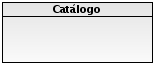
\includegraphics[width=.25\textwidth]{introduccion/images/Catalogos}
%	\end{center}
%	\label{fig:Catalogo}
%	\caption{Clase Catálogo}
%\end{figure}

%Para las demás clases actualmente se puede usar cualquier color.
%- - - - - - - - - - - - - - - - - - - - - - - - - - - - -
\subsection{Modelado de reglas de negocio}

Las reglas de negocio son directivas que tienen como fundamento la misión de un negocio y como objetivo gobernar estrategias y tácticas para poder conseguir esta misión. Una regla de negocio es practicable ya que no requiere de una interpretación adicional. Estas reglas también son una fuente de información muy relevante ya que generalmente establecen las relaciones entre dos o más términos del negocio.

En el documento se presentarán estas reglas en forma de secciones indicando los siguientes atributos:

\begin{description}
	\item[Id:] Es el identificador de la regla de negocio con la cual se podrá referenciar a lo largo del documento.
	\item[Nombre:] Indica el nombre de la regla de negocio el cual debe describir de forma concisa en que consiste la regla.
	\item[Tipo:] Indica el tipo de regla de negocio de acuerdo a como se aplica.
		\begin{itemize}
			\item Habilitadora: Permite realizar el proceso en el que la regla se ve involucrada.
			\item Cronometrada: Recibe parámetros y con respecto a eso realiza el proceso.
			\item Ejecutiva: Es aquella que se debe llevar a cabo cuando una autoridad se ve involucrada para que el proceso concluya.
		\end{itemize}
	\item[Clase:] Indica la naturaleza de la regla de negocio.
		\begin{itemize}
			\item Condición: Es una regla que cumple una condición para llevarse a cabo.
			\item Integridad Referencial: Es una regla que indica validaciones que, de no ser tomadas en cuenta se pondría en peligro la integridad de la información.
			\item Autorización: Son restricciones en las que se ven involucradas palabras como, al menos uno.
		\end{itemize}

	\item[Nivel:] Indica como es que la regla se toma en cuenta para el desarrollo del Calécac.
		\begin{itemize}
			\item Controla: Define que el sistema se encargará de vigilar el cumplimiento de la regla en todo momento.
			\item Influencia: Sugiere formas en las que debería realizarse la operación, pero no la limita. De tal forma que el sistema dará facilidades para evitar esas situaciones o advertirá cada vez que se detecte que la regla no es tomada en cuenta.
		\end{itemize}

	\item[Descripción:] Es un pequeño resumen que ayuda a entender la regla de negocio.
	\item[Motivación:] La razón detrás de la existencia de la regla de negocio.
	\item[Sentencia:] Descripción formal o matemática de la regla de negocio.
	\item[Ejemplo Positivo:] Describe ejemplos en los que la regla se cumple.
	\item[Ejemplo Negativo:] Describe ejemplos en los que la regla no se cumple.
\end{description}

%- - - - - - - - - - - - - - - - - - - - - - - - - - - - -
\section{Modelado de casos de uso}

	Los diagramas de casos de uso son una herramienta usada para representar las transacciones entre un actor y el sistema, las cuales siempre tendrán un valor agregado o un propósito para que el actor las realice.
En estos diagramas se podrán observar los siguientes elementos:

\begin{itemize}
	 \UCpaso Representa al sistema. Es un óvalo y el cómo haga las acciones definidas en las trayectoria es algo que no compete a este documento.
	\item \UCactor Representa al actor.
	\item Relación $<$- - -$<<extends>>$- - -. Indica que un caso de uso \textbf{puede} ejecutarse a partir de otro.
	\item Relación - - -$<<include>>$- - -$>$. Indica que un caso de uso \textbf{debe} ejecutarse a partir de otro.
\end{itemize}

La conexión entre un actor y un caso de uso es por medio de una línea como se muestra en la figura \ref{fig:acUC}.

\begin{figure}[hbtp!]
	\begin{center}
		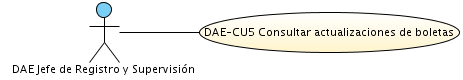
\includegraphics[width=.4\textwidth]{introduccion/images/ActorUC}
	\end{center}
	\label{fig:acUC}
	\caption{Un Actor y un caso de uso}
\end{figure}

Los casos de uso se encontrarán dentro de paquetes (representados por carpetas) indicando así que pertenecen a un mismo módulo del Calmécac como se muestra en la figura \ref{fig:pack}.

\begin{figure}[hbtp!]
	\begin{center}
		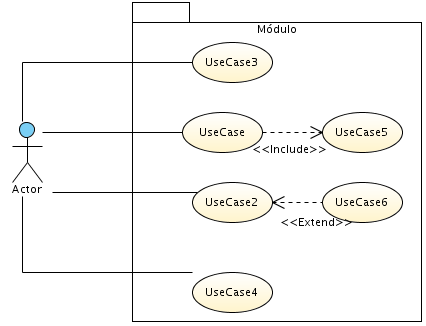
\includegraphics[width=.4\textwidth]{introduccion/images/Paquete}
	\end{center}
	\label{fig:pack}
	\caption{Un Actor con varios caso de uso dentro de un módulo}
\end{figure}

\pagebreak

%- - - - - - - - - - - - - - - - - - - - - - - - - - - - -
%\subsection{Código de colores para diagramas de casos de uso}

%Los casos de uso tendrán un color \textit{Gradient Golden} con 80\% de transparencia; los actores tendrán un  \textit{fill} \textit{RGB(122,207,245)}; los módulos del Calmécac tendrán un relleno (\textit{fill}) de color \textit{White} al 70\% de transparencia y por último el Calmécac se representa con un rectángulo de \textit{fill} \textit{RGB(128,0,0)} al 80\% de transparencia.

%- - - - - - - - - - - - - - - - - - - - - - - - - - - - -
\subsection{Identificadores de casos de uso}

Los casos de uso se identificarán de acuerdo a la siguiente nomenclatura:

\begin{figure}[hbtp!]
	\begin{center}
		
\includegraphics[width=.7\textwidth]{introduccion/images/UCnombre}
	\end{center}
	\label{fig:nomenclatura}
	%\caption{Nomenclatura de un caso de uso}
\end{figure}



En donde los subsistemas son:
\\
\begin{Titemize}
	\Titem [HR:] Horarios
	\Titem [SD:] Soporte Documental
\end{Titemize}

En donde división puede ser únicamente el módulo o el módulo puede tener submódulos.\\
 En el subsistema Horarios existe la división de módulos:\\
\begin{Titemize}
	\Titem [UA:] Unidad Académica
	\Titem [PR:] Profesor
	\Titem [EE:] Estructura Educativa
\end{Titemize}
\cdtEmpty
\\En el módulo Unidad académica se divide en submódulos:\\
\begin{Titemize}
	\Titem [GG:] Gestionar Grupo
	\Titem [CO:] Consultas
\end{Titemize}

En el subsistema Soporte Documental existe la división de módulo:\\
\begin{Titemize}
	\Titem [AP:] Aprobación
\end{Titemize}


\textbf{Ejemplo positivo} Cumple con la nomenclatura:
\begin{itemize}
	\item HR-UA-CU4 Gestionar oferta educativa
	\item HR-UA-GG-CU1.3 Asignar profesor
	\item SD-UA-CU1 Gestionar soporte documental por formatos
\end{itemize}


\textbf{Ejemplo negativo} No cumple con la nomenclatura:
\begin{itemize}
	\item CU7-UA-HR Gestionar oferta educativa
	\item GG-CU-UA3.1 Asignar profesor
\end{itemize}


%- - - - - - - - - - - - - - - - - - - - - - - - - - - - -
\subsection{Atributos de casos de uso}

Para poder entender un caso de uso más allá de un diagrama se utilizan secciones en el documento para cada uno, dividido por capítulos de acuerdo al subsistema y una tabla con los siguientes datos:

\begin{description}
	\item[Id] Identificador.
	\item[Nombre] Nombre del caso de uso el cual es descriptivo basándose en la tarea que se realiza.
	\item[Actores] Lista de los actores relacionados o que utilizan el caso de uso.
	\item[Descripción] Es un resumen en el que se especifica la transacción.
	\item[Propósito] Indica el objetivo por el cual el caso de uso existe.
	%\item[Operación:] Indica el tipo de operación que realiza el caso de uso.
	\item[Entradas] Lista los datos de entrada que el caso de uso recibe.
	\item[Salidas] Lista los datos de salida que el caso de uso genera.
	\item[Origen] Indica de donde provienen los datos de entrada.
	\item[Destino] Indica a donde se dirigen los datos de salida.
	\item[Precondiciones] Enlista las cosas que deben haber sucedido para que el caso  de uso se lleve a cabo.
	\item[Postcondiciones] Enlista las cosas que suceden en el sistema o negocio de forma inmediata o a corto plazo.
	\item[Errores] Enlista las situaciones en las que el caso de uso concluye sin éxito.
	\item[Reglas de Negocio] Lista las reglas de negocio que están asociadas al caso de uso.
%	\item[Proceso:] Enlista aquellos procesos a los que el caso de uso esta asociado.
%	\item[Subproceso:] Enlista aquellos Subprocesos en los que el caso de uso se aplica.
	\item[Disparadores] Aquellas condiciones o motivaciones que el actor tiene para ejecutar el caso de uso.
	\item[Condición de Término] Aquellos resultados que garantizan que el caso de uso se ha ejecutado con éxito.
	\item[Efectos Colaterales] Afectaciones en otras partes del sistema.
	\item[Viene de] Indica cuando el caso de uso se extiende de otro o se incluye en otro.
\end{description}

%---------------------------------------------------------
\section{Modelado de interfaces}

Una interfaz de usuario permite mostrar la interacción entre un actor y todas las funcionalidades que el sistema ofrece y que le corresponden de acuerdo a su perfil. Para poder modelar estos elementos se describe:
\begin{itemize}
	\item Objetivo: Indica el propósito de las interfaces de usuario (pantallas) y como ayudará al actor a realizar sus tareas.
	\item Descripción: En este apartado se indica y especifica que acciones el actor puede realizar así como la especificación de algunos comportamientos dinámicos en las pantallas.
\end{itemize}

%\subsection{Atributos de las interfaces}
%
%	Los diferentes atributos que se encuentran definidos a partir del capítulo \ref{part:Interaccion} de este documento. Muchos de estos elementos aun no quedan definidos, pero se utilizan símbolos con los cuales el actor pueda identificar o visualizar las acciones y funcionalidades que se pueden realizar oprimiendo estos íconos.

%---------------------------------------------------------
\section{Modelado de mensajes}

Los mensajes son elementos en el sistema que ayudan a mantener pendiente al actor, ya sea para indicarle que la operación se llevó a cabo correctamente, así como alertar de una operación que requiere realizar para poder continuar con procesos específicos realizados en el Instituto.

\subsection{Atributos de mensajes}
Un mensaje se conformará de :
\begin{description}
	\item[Tipo] Indica a que clase pertenece un mensaje, entre las cuales se encuentran:
		\begin{itemize}
			\item \textbf{Informativo:} Notificar al actor que una operación concluyó o para notificar al actor de una operación realizada en el sistema.
			\item \textbf{Confirmación:} Requiere la confirmación del actor para llevar a cabo una operación en el sistema.
			\item \textbf{Error:} Notificar al actor que la operación no se llevo a cabo adecuadamente o no se llevó a cabo.
			\item \textbf{Alerta:} Notificar al actor que una operación requiere de su atención para llevarse a cabo.
		\end{itemize}
	\item[Canal] Indica el medio que el sistema utiliza para enviar un mensaje.
	\item[Propósito] Indica la razón por la cual el mensaje es necesario.
	\item[Redacción] Indica el texto que el actor podrá visualizar cuando el mensaje se muestre.
	\item[Parámetros] Indica un elemento dentro del texto del mensaje que puede cambiar dinámicamente de acuerdo a la operación que se este llevando a cabo.
	\item[Ejemplo] Muestra una aplicación del mensaje.
	\item[Referenciado por] Indica la lista de casos de uso que utilizan el mensaje.
\end{description}

\subsection{Identificadores de mensajes}
Para poder identificar un mensaje, este se compondrá de:
\begin{description}
	\item [Identificador] Indica el número asignado para el mensaje.
	\item [Nombre] Es un resumen de lo que el mensaje realiza/muestra.
\end{description}

        
        
        %%%%%%%%%%%%%%%%%%%%%%%%%%%%%%%%%%%%%%%%%%%%%%%%%%%%%%%%%%%%%%%%
        % Primera Parte: Modelado del negocio.
        \part{Modelado del negocio}
        \label{ch:modeloNegocio}
        
        %---------- Glosario ----------
        \chapter{Glosario}
        \label{ch:glosario}
        El presente glosario presenta los términos utilizados a lo largo del documento. Esta unificación de criterios está basada en la normatividad y cultura del IPN y tiene como finalidad establecer el lenguaje base que permita comprender la especificación del sistema y se utilizará en la construcción del mismo.

\section{Glosario de términos}
\begin{bGlosario}
	%------------------------------------------------------------
	\bTerm{tAcademia}{Academia} Al órgano constituido por profesores que tiene la finalidad de proponer, analizar, opinar, estructurar y evaluar el proceso educativo.
	%------------------------------------------------------------
	%\bTerm{tActividadDentroDelPeriodoEscolar}{Actividades dentro del Periodo Escolar} Se refiere a Periodos\footnote{\refElem{tPeriodo}.} y fechas marcadas en el \refElem{tCalendarioEscolar} del IPN a realizarse dentro de los Periodos Escolares\footnote{\refElem{tPeriodoEscolar}}. Las cuales son:
  %  \begin{itemize}
	%	\item \refElem{tRegistroDeEvaluacionOrdinaria}.
	%	\item \refElem{tRegistroDeEvaluacionExtraordinaria}.
	%	\item \refElem{tSistemaDeInduccion}.
	%	\item \refElem{tSuspensionDeLabores}.
	%	\item \refElem{tRegistroDeEvaluacionPorSaberesPreviamenteAdquiridos}.
  %  \end{itemize}
	%------------------------------------------------------------
	%\bTerm{tActividadFueraDelPeriodoEscolar}{Actividades fuera del Periodo Escolar} Se refiere a Periodos\footnote{\refElem{tPeriodo}.} y fechas marcadas en el \refElem{tCalendarioEscolar} del IPN a realizarse fuera de los Periodos Escolares\footnote{\refElem{tPeriodoEscolar}}. Las cuales son:
	%\begin{itemize}
	%	\item \refElem{tAplicacionETS}.
	%	\item \refElem{tActividadIntersemestral}.
	%	\item \refElem{tVacaciones}.
	%\end{itemize}
	%------------------------------------------------------------
	%\bTerm{tActividadIntersemestral}{Actividad Intersemestral} Se refiere a las actividades realizadas por profesores\footnote{\refElem{tProfesor}}
	%una vez que el período escolar ha terminado. %% Propuesta.
	%------------------------------------------------------------
	\bTerm{tAlumno}{Alumno} A la persona inscrita en algún programa académico que se imparta en cualquier nivel educativo y	modalidad educativa
	que ofrece el Instituto Politécnico	Nacional. %% RGE
 	%------------------------------------------------------------
 	\bTerm{tAntecedenteAcademico}{Antecedente Académico} Conjunto de unidades de aprendizaje necesarias que sirven como fundamento o de apoyo
	para cursar otra de un semestre o nivel más alto %Derivado verificar redacción
 	%------------------------------------------------------------
 	%\bTerm{tAplicacionETS}{Aplicación de Examen a Título de Suficiencia} A la aplicación de los Exámenes a Título de Suficiencia\footnote{\refElem{tETS}}. %Derivada

 	%-----------------------------------------------------------
 	\bTerm{tAreaFormacion}{Área de Formación} Conjunto de conocimientos que por su afinidad conceptual, teórica y metodológica, conforman
	una porción claramente identificable de los contenidos de un plan de estudios en una carrera tecnológica, técnica superior o de grado.
	Pueden identificarse con áreas de conocimientos disciplinares, áreas temáticas, experiencias de formación, etc. En el Instituto se definen tres tipos de áreas de formación:
	\begin{itemize}
		\item Institucional.
		\item Científica, Humanística y Tecnológica Básica.
		\item Profesional.
	\end{itemize}

 	%-----------------------------------------------------------
 	%\bTerm{tCalendarioEscolar}{Calendario Escolar} Conjunto de calendarios de un año (también llamado \refElem{tCicloEscolar}) que inicia en agosto
	%de un año y termina en agosto del siguiente. En donde se marcan los Periodos Escolares\footnote{\refElem{tPeriodoEscolar}} de todas las
	%Modalidades\footnote{\refElem{tModalidad}} y todas las fechas relevantes (ya sea \refElem{tActividadDentroDelPeriodoEscolar} o
	%\refElem{tActividadFueraDelPeriodoEscolar}).
 	%----------------------------------------------------------
 	\bTerm{tCargaMaxima}{Carga máxima en Créditos} Resultado de dividir el número total de créditos del programa académico entre el número de
	periodos escolares de la duración mínima del plan de estudio.
 	%-----------------------------------------------------------
 	\bTerm{tCargaMedia}{Carga media en Créditos} Resultado de dividir el número total de créditos del programa académico entre el número
	de periodos escolares de la duración establecida en el plan de estudio.
 	%----------------------------------------------------------
 	\bTerm{tCargaMinima}{Carga mínima en Créditos} Resultado de dividir el número total de créditos del programa académico entre
	el número de periodos escolares de la duración máxima del plan de estudio.
 	%------------------------------------------------------------
 	\bTerm{tCarrera}{Carrera} ver \refElem{tProgramaAcademico}.
 	%-----------------------------------------------------------
	%\bTerm{tCicloEscolar}{Ciclo Escolar} El lapso anual que define el calendario académico
 	%----------------------------------------------------------
	\bTerm{tCompetencia}{Competencia}  Es la posibilidad de movilizar e integrar diversos saberes y recursos cognitivos cuando se
	enfrenta una situación-problema inédita, para lo cual la persona requiere mostrar la capacidad de resolver problemas complejos y abiertos,
	en distintos escenarios y momentos. permite identificar, seleccionar, coordinar y movilizar de manera articulada e interrelacionada un
	conjunto de saberes diversos en el marco de una situación educativa en un contexto específico.
	%-----------------------------------------------------------
	\bTerm{tCompetenciaGeneral}{Competencia General} Es la \refElem{tCompetencia} que se busca adquirir al finalizar una \refElem{tUnidadDeAprendizaje}.
	%-----------------------------------------------------------
 	\bTerm{tCredito}{Crédito} A la unidad de reconocimiento académico que mide y cuantifica las actividades de
	aprendizaje contempladas en un plan de estudio; es universal, transferible entre programas académicos y equivalente al
	trabajo académico del alumno.
 	%----------------------------------------------------------
 	\bTerm{tCreditosSATCA}{Créditos SATCA}  Es  un  conjunto  de  criterios  simples  y  unívocos  para
 	asignar  valor  numérico  a  todas  las actividades  de  aprendizaje  del  estudiante  contempladas  en  un  plan  de  estudios, con la finalidad
	de acumular y transferir créditos académicos.
 	%----------------------------------------------------------
 	\bTerm{tCreditosTEPIC}{Créditos TEPIC} Es la unidad de valor o puntuación de una asignatura, que se calcula de la siguiente forma:
 	\begin{enumerate}
 		\item  En actividades que requieren estudio o trabajo adicional del alumno, como en las clases teóricas y en los seminarios, una hora de
		clase-semana-semestre corresponde a dos créditos.
 		\item En actividades que no requieren estudio o trabajo adicional del alumno, como las prácticas, los laboratorios y los talleres,
		una hora-semana-semestre corresponde a un crédito.
 		\item  El valor en créditos de actividades clínicas y de las prácticas para el aprendizaje de la música, las artes plásticas y las
		asignaturas de preparación para el trabajo, se computarán globalmente según su importancia en el plan de estudios y a criterio de los cuerpos
		académicos correspondientes.
 	\end{enumerate}
	%----------------------------------------------------------
 	%\bTerm{tETS}{Examen a Título De Suficiencia} Es la evaluación que comprende el total de los contenidos del programa de estudios y que el alumno podrá presentar cuando no haya acreditado de manera ordinaria o extraordinaria alguna unidad de aprendizaje.
 	%----------------------------------------------------------
 	%\bTerm{tEvaluacionExtraordinaria}{Evaluación Extraordinaria}A la que comprende el total de los contenidos del programa de estudios y que el alumno podrá presentar voluntariamente, dentro del mismo periodo escolar, una vez que cursó la unidad de aprendizaje y no haya obtenido un resultado aprobatorio, o bien, si habiéndola acreditado, desea mejorar su calificación.
 	%------------------------------------------------------------
 	%\bTerm{tEvaluacionOrdinaria}{Evaluación Ordinaria}A la que se presenta con fines de acreditación durante el periodo escolar y
	%considera las evidencias de aprendizaje señaladas en el programa de estudios.
 	%-----------------------------------------------------------
	\bTerm{tEvidenciaIntegradora}{Evidencia Integradora} Elemento didáctico utilizado como evidencia de que el \refElem{tAlumno} adquirio el conocimiento
	o alcanzó una \refElem{tCompetencia}.%Verificar redaccción.
	%-----------------------------------------------------------
 	\bTerm{tFundamentacion}{Fundamentación} Redacción que le sirve de apoyo al \refElem{tProgramaDeEstudios} de una \refElem{tUnidadDeAprendizaje}
	para justificar su incorporación a un \refElem{tProgramaAcademico}.
 	%----------------------------------------------------------
	\bTerm{tIntencionEducativa}{Intención Educativa} Objetivos  específicos  definidos  en términos  de  actividades
	pedagógicas  en  el  nivel  de  la  secuencia de  aprendizaje;  permiten  la realización  concreta  de  los  saberes  bajo  la  forma
	de una  serie  de  adquisiciones  escolares (saber, saber ser, saber hacer, actitudes y valores).
	%----------------------------------------------------------
 	\bTerm{tISBN}{ISBN} Un ISBN es un código normalizado internacional para libros (International Standard Book Number). Los ISBN
	tuvieron 10 dígitos hasta diciembre de 2006 pero, desde enero de 2007, tienen siempre 13 dígitos. Los ISBN se calculan utilizando una
	fórmula matemática específica e incluyen un dígito de control que valida el código.
 	%------------------------------------------------------------
 	\bTerm{tISSN}{ISSN} Código de 8 dígitos usado para identificar periódicos, journals, revistas y publicaciones periódicas de todo tipo y
	en media-print y electrónico.
 	%------------------------------------------------------------
 	\bTerm{tMapaCurricular}{Mapa Curricular} A la representación gráfica de las unidades de aprendizaje que conforman un plan de estudio.
 	%------------------------------------------------------------
 	\bTerm{tModalidad}{Modalidad} Determina la forma en que debe impartirse una \refElem{tUnidadDeAprendizaje}, \refElem{tProgramaAcademico} o
	en que un \refElem{tAlumno} está llevando su \refElem{tCarrera}. Existen tres modalidades en el Instituto:
 	\begin{Citemize}
 		\item \refElem{tModalidadPresencial}.
 		\item \refElem{tModalidadMixta}.
 		\item \refElem{tModalidadADistancia}.
 	\end{Citemize}
 	%------------------------------------------------------------
	\bTerm{tModalidadPresencial}{Modalidad Presencial}  La que se desarrolla en aulas, talleres, laboratorios y otros ambientes de aprendizaje, en
	horarios y periodos determinados. A esta modalidad generalmente también se le conoce como Modalidad Escolarizada.
 	%------------------------------------------------------------
	\bTerm{tModalidadMixta}{Modalidad Mixta} Es la combinación de modalidades educativas de acuerdo con el diseño un programa académico en particular.
 	%------------------------------------------------------------
	\bTerm{tModalidadADistancia}{Modalidad a Distancia}	Es la que se desarrolla fuera de las aulas, talleres, laboratorios y no
	necesariamente comprende horarios determinados. A esta modalidad generalmente también se le conoce como Modalidad No Escolarizada.
 	%------------------------------------------------------------
	\bTerm{tOrientacionDidactica}{Orientación Didáctica} Instrumentos que sirven para clasificar y especificar la forma en que una
	\refElem{tUnidadDeAprendizaje} debe ser impartida.
	%------------------------------------------------------------
 	\bTerm{tPaginaElectronica}{Página Electrónica} Documento en internet que contiene la información de las unidades de
	aprendizaje\footnote{ver \refElem{tUnidadDeAprendizaje}}.
 	%------------------------------------------------------------
 	\bTerm{tPlanEstudio}{Plan de Estudio} Estructura curricular que se deriva de un programa académico y que
	permite cumplir con los propósitos de formación general, la adquisición de conocimientos y el desarrollo de capacidades
	correspondientes a un nivel y modalidad educativa.%Reglamento General de Estudios
 	%------------------------------------------------------------
 	\bTerm{tPerfilDocente}{Perfil Docente} Requisitos que sirve den apoyo al \refElem{tProgramaDeEstudios} de una \refElem{tUnidadDeAprendizaje}
	para definir el perfil con el que un \refElem{tProfesor} debe(o sugiere) tener para impartir una \refElem{tUnidadDeAprendizaje}.
% 	%------------------------------------------------------------
% 	\bTerm{tPeriodo}{Periodo} Se refiere a un lapso de tiempo el cual está marcado por una fecha de inicio y una fecha final.
% 	%------------------------------------------------------------
% 	\bTerm{tPeriodoEscolar}{Periodo Escolar} Se refiere al \refElem{tPeriodo} que rige la ejecución de todas las actividades relevantes en la gestión escolar. En la modalidad presencial tiene una duración aproximada de seis meses y en modalidad mixta seis semanas.
 	%------------------------------------------------------------
 	\bTerm{tPeriodoDeTrabajo}{Periodo de Trabajo} Lapso de tiempo en que una unidad de aprendizaje debe impartirse puede ser:
 		\begin{itemize}
 			\item Mensual.
 			\item Bimestral.
 			\item Trimestral.
 			\item Cuatrimestral.
 			\item Semestral.
 			\item Anual.
 		\end{itemize}
 	
 	%------------------------------------------------------------
 	\bTerm{tPractica}{Práctica} Elemento didáctico para ayudar y dar soporte al conocimiento adquirido de una \refElem{tUnidadDeAprendizaje}.
 	%-----------------------------------------------------------
 	\bTerm{tProfesor}{Profesor} Persona que conduce el proceso de enseñanza-aprendizaje enfocado a la transmisión de conocimientos y a
	la formación integral del alumno. Será la autoridad académica del grupo a su cargo y desempeñará sus actividades conforme al
	principio de libertad de cátedra e investigación, atendiendo los programas aprobados por las autoridades académico-administrativas del
	IPN y del centro de trabajo correspondiente.
 	%------------------------------------------------------------
 	\bTerm{tPolivirtual}{Polivirtual} Es el sistema del Instituto Politécnico Nacional mediante el cual ofrece estudios
	de bachillerato, licenciatura, posgrado y servicios educativos complementarios en modalidades alternativas, innovadoras y
	flexibles con apoyo de las tecnologías de la información y las comunicaciones.
 	%------------------------------------------------------------
	\bTerm{tProgramaAcademico}{Programa Académico} Conjunto organizado de elementos necesarios para generar, adquirir y aplicar
	el conocimiento en un campo específico; así como para desarrollar habilidades, actitudes y valores en el alumno, en diferentes
	áreas del conocimiento. %Reglamento General de Estudios
 	%------------------------------------------------------------
 	\bTerm{tProgramaDeEstudios}{Programa de Estudios} Contenidos formativos de una unidad de aprendizaje contemplada en un plan de estudio;
	especifica los objetivos a lograr por los alumnos en un periodo escolar; establece la carga horaria,
	número de créditos, tipos de espacios, ambientes y actividades de aprendizaje, prácticas escolares, bibliografía, plan de evaluación y
	programa sintético.
 	%-----------------------------------------------------------
 	\bTerm{tProgramaEnRed}{Programa Académico en Red} Programa que desarrollan e imparten conjuntamente varias unidades académicas del Instituto
 	o con otras instituciones con las que se tenga convenio.
 	%------------------------------------------------------------
 	\bTerm{ramaConocimiento}{Rama del Conocimiento} Es la clasificación designada para un \refElem{tProgramaAcademico} de nivel
	superior o medio superior. Dentro del Instituto se encuentran :
	\begin{itemize}
	\item Ciencias Físico Matemáticas.
	\item Ciencias Médico Biológicas.
	\item Ciencias Sociales y Administrativas.
	\end{itemize}
 	%----------------------------------------------------------
 	\bTerm{tRAP}{Resultado de Aprendizaje Propuesto} También conocidas como RAP's, se abordan a través de actividades sustantivas que tienen como
	propósito indicar una generalidad para desarrollar las secuencias didácticas que atenderán cada RAP.
	Las evidencias con las que se evaluará formativamente cada RAP, se definen mediante un desempeño integrado, en el que
	los estudiantes mostrarán su saber hacer de manera reflexiva, utilizando el conocimiento que va adquiriendo durante el proceso
	didáctico para transferir el aprendizaje a situaciones similares y diferentes.
 	%------------------------------------------------------------
 	\bTerm{tReferenciaDocumental}{Referencia Documental} Bibliografía sugerida para ocuparse durante el curso de una \refElem{tUnidadDeAprendizaje} de nivel
	medio superior.

 	%---------------------------------------------------------------
 	%\bTerm{tRegistroDeEvaluacionOrdinaria}{Registro de Evaluación Ordinaria} Periodos\footnote{\refElem{tActividadDentroDelPeriodoEscolar}} marcados como \refElem{tPeriodo}. en los que se permite o requiere a los profesores subir calificaciones\footnote{\refElem{tEvaluacionOrdinaria}.} de sus alumnos. Tradicionalmente existen tres periodos en modalidad \refElem{tModalidadPresencial} y uno en modalidad \refElem{tPolivirtual}.
 	%------------------------------------------------------------
 	%\bTerm{tRegistroDeEvaluacionExtraordinaria}{Registro de Evaluación Extraordinaria} \refElem{tActividadDentroDelPeriodoEscolar} marcada como \refElem{tPeriodo} en el que se requiere a los profesores registrar las evaluaciones extraordinarias\footnote{\refElem{tEvaluacionExtraordinaria}} de sus alumnos.
 	%------------------------------------------------------------
 	%\bTerm{tRegistroDeEvaluacionPorSaberesPreviamenteAdquiridos}{Registro de Evaluación por Saberes Previamente Adquiridos} \refElem{tActividadDentroDelPeriodoEscolar} marcada como fecha la cual determina el día máximo en el que se puede registrar calificaciones derivadas de \refElem{tSaberesPreviamenteAdquiridos}.
	%------------------------------------------------------------
 	%\bTerm{tSaberesPreviamenteAdquiridos}{Saberes Previamente Adquiridos}A la que permite acreditar unidades de aprendizaje sin haberlas cursado. Su aplicación se sujetará a lo descrito en el plan y programa de estudios, y a los lineamientos aplicables.
 	%------------------------------------------------------------
 	%\bTerm{tSistemaDeInduccion}{Semana de Inducción} \refElem{tActividadDentroDelPeriodoEscolar} marcada como \refElem{tPeriodo} en el que las Unidades Académicas\footnote{\refElem{tUnidadAcademica}} deben dar información de orientación e inducción a los aspirantes asignados.
 	%------------------------------------------------------------
 	%\bTerm{tSuspensionDeLabores}{Suspensión de labores} \refElem{tActividadDentroDelPeriodoEscolar} marcadas como fechas específicas en las que se suspenden las labores académicas. En principio, su definición está basada en los días de descanso marcados por la secretaría del trabajo y por el calendario escolar de la Secretaría de Educación Pública.
 	%------------------------------------------------------------
	\bTerm{tTipoEspacio}{Tipo de Espacio} Para nivel medio superior, indica en que lugar la \refElem{tUnidadDeAprendizaje} se imparte. Puede ser:
		\begin{itemize}
			\item Aula.
			\item Taller.
			\item Laboratorio.
			\item Otros ambientes de aprendizaje.
		\end{itemize}
	%------------------------------------------------------------
	\bTerm{tUnidadAcademica}{Unidad Académica} Espacio geográfico donde se ubican las escuelas, centros y unidades en los que se realizan actividades de docencia, investigación y difusión de la cultura, en los niveles superior y de posgrado.
 	%------------------------------------------------------------
 	\bTerm{tUnidadDeAprendizaje}{Unidad de Aprendizaje} Estructura didáctica que integra los contenidos formativos de un curso, materia, módulo, asignatura o sus equivalentes. En general, las unidades de aprendizaje deberán cursarse y acreditarse conforme lo establezca el plan de estudio, y podrán seleccionarse de entre la oferta disponible en el periodo escolar y sujeta a grupo. %Reglamento General de Estudios
 	%------------------------------------------------------------
 	\bTerm{tUnidadDidactica}{Unidad Didáctica} Elementos que definen y componen a una \refElem{tUnidadDeAprendizaje} de nivel medio superior.
 	%------------------------------------------------------------
 	\bTerm{tUnidadTematica}{Unidad Temática} Elementos que definen y componen a una \refElem{tUnidadDeAprendizaje} de nivel superior.
 	%------------------------------------------------------------
 	%\bTerm{tVacaciones}{Vacaciones} Descanso temporal de una actividad habitual, principalmente del trabajo remunerado o de los estudios. %RAE


 	%------------------------------------------------------------
%	\bTerm{tCarrera}{}
% 	%------------------------------------------------------------
%	\bTerm{tUnidadDeAprendizaje}{}
% 	%------------------------------------------------------------
%	\bTerm{tProgramaAcademico}{}
% 	%------------------------------------------------------------
%	\bTerm{tAlumno}{}


%	\bTerm{tAlta}{Alta} Documento que acredita y reconoce la inscripción. %MP DAE
%
%	\bTerm{tAlumnoRegistradoEnSIRCEI}{Alumno Registrado en SIRCEI} Alumno del nivel medio superior o superior, reconocido en el Sistema de Registro y Control Escolar Institucional, para su control y seguimiento a su trayectoria académica, y consulta de calificaciones, vía internet.x %MP DAE
%
%	\bTerm{tAntecedentesDeIngreso}{Antecedentes de Ingreso} Reseña de la Admisión del alumno en la Institución. % MP DAE
%
%	\bTerm{tAntecedentesDeTrayectoria}{Antecedentes de Trayectoria} Situación del alumno que ha llevado una dirección dentro del Instituto a lo largo del tiempo. % MP DAE
%
%	\bTerm{AspiranteAceptado}{Aspirante Aceptado} Aspirante que al haber aprobado el examen de admisión y que cumple con los requisitos establecidos en la convocatoria correspondiente es asignado a una unidad académica. %Derivado
%
%	\bTerm{tAspiranteAExaminar}{Aspirante a Examinar}Persona que se registra en el proceso de admisión para ingresar a alguna de las escuelas, centros y unidades del Instituto, en los niveles que constituyen su oferta educativa. %MP DAE
%
%	\bTerm{tBoleta}{Boleta}Cédula de identidad que se otorga a los aspirantes, para que se inscriban como alumnos del Instituto Politécnico Nacional. %MP DAE
%
%	\bTerm{Cadena}{Cadena} Es el Tipo de Dato definido por cualquier valor que se componga de una secuencia de caracteres, con o sin acentos, espacios, dígitos y signos de puntuación. Existen tres tipos de Cadenas: Palabra, Frase y Párrafo.
%
%	\bTerm{tCalendarioAcademico}{Calendario Académico} Programación que define los tiempos en los cuales se realizan anualmente las actividades académicas y de gestión escolar, en las diversas modalidades educativas que se imparten en el Instituto
%
%	\bTerm{tCicloEscolar}{Ciclo Escolar} El lapso anual que define el calendario académico
%
%	\bTerm{tConvocatoria}{Convocatoria} Documento de carácter oficial emitido por una o varias Instituciones Educativas, en el cual se plantea tanto el procedimiento, los tiempos y fechas, los
%	lineamientos legales en los que se basa la misma, y los requisitos que hay que cumplir para que un aspirante sea admitido al nivel de estudios superior inmediato concluido por él mismo, en la o las Instituciones que ofrecen sus distintas carreras y niveles de estudios impartidos por las mismas. % MP DAE
%
%	\bTerm{tCredencialDeAlumno}{Credencial de Alumno} Identificación oficial expedida por la Dirección de Administración Escolar del IPN, para todos aquellos alumnos que cursan alguna carrera en uno de los planteles educativos del Instituto, ya sea a Nivel Medio Superior o Superior. %MP DAE
%
%	\bTerm{Entero}{Entero} Es el Tipo de Dato definido por todos los valores numéricos enteros, tanto positivos como negativos.
%
%	\bTerm{tEstructuraAcademica}{Estructura Académica} Al conjunto de grupos, horarios y unidades de aprendizaje organizadas para el período siguiente.
%
%	\bTerm{tETS}{Examen a Título De Suficiencia} Es la evaluación que comprende el total de los contenidos del programa de estudios y que el alumno podrá presentar cuando no haya acreditado de manera ordinaria o extraordinaria alguna unidad de aprendizaje.
%
%	\bTerm{tExpedienteAcademico}{Expediente Académico} Al documento que contiene la información y el historial académico del alumno.
%
%	\bTerm{tExpedienteDelAspirante}{Expediente del Aspirante} Se refiere a la documentación que el aspirante entrega durante el proceso de admisión para su verificación. % Derivado
%
%	\bTerm{Fecha}{Fecha} Es el Tipo de Dato definido por todas las fecha pasadas y futuras. Se representa de dos formas: Fecha Corta y Fecha Larga.
%
%	\bTerm{FechaCorta}{Fecha corta} Representación de una fecha de la forma DD/MM/YYYY, ejemplo: 24/02/2012.
%
%	\bTerm{FechaLarga}{Fecha Larga} Representación de una fecha de la forma DD de MMMM, del YYYY, ejemplo: 24 de Febrero, del 2012.
%
%	\bTerm{Frase}{Frase} Cadena formada por mas de una palabra y que puede ocupar hasta un par de renglones.
%
%	\bTerm{tHistorialAcademico}{Historial Académico} Se entiende por historial académico al conjunto de calificaciones obtenidas por un alumno en las unidades de aprendizaje,durante su vida académica dentro del Instituto.
%
%	\bTerm{tHojaDeResultadoDelExamenDeAdmision}{Hoja de Resultado del Examen de Admisión} Documento que el interesado imprime a través de internet, para conocer la opción educativa donde quedó aceptado. Con la Hoja de Resultados los aspirantes seleccionados obtendrán una cita donde podrán continuar con sus trámites de inscripción al Instituto. %MP DAE
%
%	\bTerm{tHorario}{Horario} Documento que se le otorga a un aspirante o alumno en el que se confirma su inscripción al período en curso.
%
%	\bTerm{tIncidencia}{Incidencia}Acontecimiento que sobreviene en el curso de un asunto o negocio y tiene con él alguna conexión.
%
%
%	\bTerm{tKardex}{Kardex} Documento donde se resgistran los datos personales del alumno, el cual contiene la trayectoria escolar mediante las calificaciones obtenidas en las asignaturas y/o unidades de aprendizaje cursadas, de acuerdo a un plan de estudios, formas de evaluación y periodos escolares. % CIRCULAR NO5 Criterios de Expedición de Boletas de calificaciones
%
%	\bTerm{tModalidad}{Modalidad Educativa} Forma en que se organizan, distribuyen y desarrollan los planes y programas de estudio para su impartición. Existen 3 tipos de modalidades:
%	\begin{itemize}
%		\item [Escolarizada:] La que se desarrolla en aulas, talleres, laboratorios y otros ambientes de aprendizaje, en horarios y periodos determinados.
%		\item [No Escolarizada:] Es la que se desarrolla fuera de aulas,
%		talleres, laboratorios y no necesariemente comprende horarios determinados.
%		\item [Mixta:] Es la combinación de modalidades educativas de
%		acuerdo con el diseño un programa académico en particular.
%	\end{itemize}
%
%	\bTerm{tNombramiento}{Nombramiento} Proceso por el cual un aspirante a dar cátedra en el instituto es elegido otorgándole las horas que deberá cumplir. % RCITPAIPN
%
%
%	\bTerm{tOficioDeAlumnoAceptado}{Oficio de Alumno Aceptado} Documento generado por la Dirección de Administración Escolar del IPN, por medio del cual el aspirante es notificado que al concluir los trámites de inscripción adquiere el estatus de alumno del Instituto. % MP DAE
%
%
%	\bTerm{tPreboleta}{Preboleta} Es un numéro de identificación que se le asgina al aspirante como fin de control interno durante el proceso de admisión. %Derivado
%
%	\bTerm{tProcesoDeAdmision}{Proceso de Admisión} Conjunto de etapas que deben ser realizadas tanto por la Institución educativa como por el aspirante. Comprende desde la publicación de la convocatoria, el regist ro de aspirantes, la aplicación del examen de admisión, publicación de resultados e inscripciones de aspirantes seleccionados. %MP DAE
%
%
%
%	\bTerm{RCITPAIPN}{Reglamento de  las  Condiciones Interiores de Trabajo del Personal Académico del IPN} Reglamento que fija las condiciones de trabajo del personal académico del
%	Instituto Politécnico Nacional, que conjuntamente con sus tres anexos:
%	\begin{itemize}
%		\item[I.] Prestaciones Sociales y Económicas.
%		\item[II.] Seguridad e Higiene.
%		\item[III.] Promoción Docente.
%	\end{itemize}
%	Son de observancia obligatoria para el personal académico, el titular y demás funcionarios del Instituto
%	Politécnico Nacional y de sus Organos de Apoyo.
%
%	\bTerm{tRUAA}{Registro Único de Actividades Académicas } Es  el  documento  que  avala  las  funciones  y  actividades  que  desarrolla  el  docente
%
%	\bTerm{tTrayectoriaEscolar}{Trayectoria Escolar} Al proceso a través del cual el alumno construye su formación con base en un plan de estudio.
%
%
%
%	\bTerm{tValidacionDeInscripcion}{Validación de Inscripción} Proceso a través del cual se dictamina la autenticidad y legitimidad de los documentos aportados por el aspirante para su inscripción, si la documentación es correcta se le comunica por escrito. %MP DAE
%


	% TODO:Agregar fuente


\end{bGlosario}

        
        %---------- Modelo de Tipos de Datos ----------
        \chapter{Modelo de Tipos de Datos}
        \label{ch:tipos}
        En este capítulo se definen aquellos datos que son utilizados a lo largo del documento y que ayudan a comprender las características de  cada uno de los atributos que son 
utilizados en el modelo de información, casos de uso e interfaces. Se podrán observar distintas entidades qe psoiblemente no se 
encuentren en el modelo de información del componente.

	\begin{TipoDeDato}{tdentero}{Entero}{Cualquier elemento del conjunto formado por los números naturales, sus opuestos (versiones negativas de los naturales) y el cero. Estos números pueden ser\{0,1,2,3,4,5,6,7,8,9\} y todos los que se forman a partir de ellos.}
\end{TipoDeDato}

\begin{TipoDeDato}{tdflotante}{Flotante}{Es cualquier elemento del conjunto formado por los números reales, sus opuestos (versiones negativas de los reales) y el 0. Tiene como propósito representar valores fraccionales de alta precisión.}
\end{TipoDeDato}

\begin{TipoDeDato}{tdbooleano}{Booleano}{Es un \refElem{tTipoDato} lógico que representa lógica binaria, o que admite solo dos valores los cuales son:
		\begin{Citemize}
			\item \textbf{Verdadero} generalmente representado como T o como un uno(1).
			\item \textbf{Falso} Generalmente representado como F o como un cero(0).
		\end{Citemize}}
\end{TipoDeDato}

\begin{TipoDeDato}{tdpalabra}{Palabra}{Es un dato que se compone por una cadena de caracteres alfanuméricos, aceptando tanto mayúsculas, minúsculas del alfabeto y todos los dígitos que se pueden formar con los números 0,1,2,3,4,5,6,7,8 y 9 así como caracteres especiales como el ., @ , etc.}
	\begin{Citemize}
		\item \textbf{Restricciones}: La cadena no puede tener espacios.
		\item \textbf{Longitud}: Su longitud es de 0 a 20 caracteres.
	\end{Citemize}	
\end{TipoDeDato}
	
\begin{TipoDeDato}{tdfrase}{Frase}{Es un dato que se compone por varias cadenas, o palabras separadas por espacios o signos de puntuación.\\}
		\textbf{Longitud}: Su longitud es de 20 a 200 caracteres
\end{TipoDeDato}
	
	
\begin{TipoDeDato}{tdparrafo}{Párrafo}{Es un dato que se compone por varias frases, separadas por espacios o signos de puntuación.\\}
		 \textbf{Longitud}: Su longitud es de 200 a 1000 caracteres.
\end{TipoDeDato}
		
\begin{TipoDeDato}{tdtexto}{Texto}{Es un dato que se compone por varios párrafos. Este tipo de dato se utiliza con el fin de transmitir un mensaje complejo.\\}
		\textbf{Longitud}: Su longitud es de 1000 a 80000 caracteres.

\end{TipoDeDato}
		
\begin{TipoDeDato}{tdfecha}{Fecha}{Es un tipo de dato que se compone de 3 atributos  en el que se realiza la especificación de día, mes y año de una fecha particular de un año . }

	\textbf{Formatos}: \cdtEmpty
		\begin{Citemize}
			\item Fecha Corta: Es la descripción de una fecha y se presenta de la siguientes formas:
				\begin{itemize}
					\item \textit{12-12-17}
					\item \textit{12/12/17}
				\end{itemize} 
			Ambas formas son correctas. En el primer campo se establece el día, en el segundo el mes y en el último el año. Para el ejemplo propuesto entonces la fecha corta indicaría el día 12 del mes de diciembre del año 2017.
			
			\item Fecha Larga: Es la descripción de una fecha y se presenta de la siguiente forma:
				\textit{12 de Diciembre del 2017}.
		\end{Citemize}
\end{TipoDeDato}

	\begin{TipoDeDato}{tdhora}{Hora}{Es un tipo de dato que se compone de 2 atributos  en el que se realiza la especificación de hora y minutos separados por dos puntos. Este tipo de dato se utiliza para la representación de un momento específico del día.}

		 \textbf{Formatos}:\cdtEmpty
		\begin{Citemize}
		
			\item Formato 24 hrs : Es la descripción de una hora, la cual se presenta de la siguiente forma: \textit{13:30hrs}. Para el ejemplo propuesto la hora indicaría las 13 horas y media.
				\begin{itemize}
					\item \textbf{Restricciones:} En los campos que sea requerido este formato, se debe validar que el número que corresponde a los minutos no sobrepase el valor \textit{59} y que el número que corresponde a las horas no sobre pase el valor de \textit{24}
				\end{itemize}
			
			\item Formato p. m. /a. m. : Es la descripción de una hora, la cual se presenta de la siguiente forma: \textit{1:30 p.m.}. Para el ejemplo propuesto la hora indicaría la 1 y media de la tarde.Esto con base en el sistema de 12 horas que específica :
				\begin{itemize}
					\item \textbf{a. m. } Significa \textit{ante meridiem} o ``Antes del mediodía''. 
					\item \textbf{p. m. } Significa \textit{post meridiem} o ``Después del mediodía''.
				\end{itemize}
		\end{Citemize}
\end{TipoDeDato}

		\begin{TipoDeDato}{tdarchivo}{Archivo}{Este tipo de dato permite el almacenamiento de documentos en en el sistema.}
		\textbf{Formatos}: El sistema puede soportar los siguientes formatos de archivo:
				\begin{Citemize}
					\item \textbf{JPEG}(y derivados: JPG,JFIF,JPX,JP2): Formato para el almacenamiento de imágenes.
					\item \textbf{PDF}: Es un formato que provee de imágenes, texto o imagenes y texto.
					\item \textbf{PNG}: Formato para el almacenamiento de imágenes.
				\end{Citemize}
\end{TipoDeDato}
			
%Catálogos Básicos
	 
\begin{TipoDeDato}{tdGradoAcademico}{Grado Académico}{Es un catálogo que tiene como utilidad almacenar todas las posibles distinciones académicas que profesores y alumnos adquieren a lo largo de su trayectoria académica dentro o fuera del Instituto.}
		 \begin{tdAtributos}
		 	\tdAttr{nombre}{Nombre}{tdfrase}{Es la palabra o el conjunto de palabras que identifican a una distinción académica otorgada por una Institución Educativa(Nacional o Internacional).}
	 		\tdAttr{abreviatura}{Abreviatura}{tdpalabra}{Es el símbolo o conjunto de símbolos que tienen como propósito representar el nombre de una distinción académica por medio de una clave.}
		 \end{tdAtributos}
		 
	 \subsection{Valores Iniciales}
	 	 En la siguiente tabla se muestran aquellos valores con los cuales el catálogo será poblado inicialmente.\cdtEmpty
	 		\begin{longtable}{| p{0.3\textwidth}| p{0.3\textwidth}|}
	 			\rowcolor{colorPrincipal}
	 			\multicolumn{2}{|c|}{\bf \color{white} Valores Iniciales}\\
	 			\hline
	 			\rowcolor{colorSecundario}
	 			\bf \color{white} Grado & \bf \color{white} Abreviatura \\
	 			\hline
	 			Licenciatura & Lic.\\
	 			\hline
	 			Maestría & M. \\
	 			\hline
	 			Doctorado & Dr. \\
	 			\hline
	 		\end{longtable}
	 \end{TipoDeDato}

	\begin{TipoDeDato}{tdDia}{Día}{Es un catálogo en el que se almacena información de los 7 días de la semana de acuerdo al calendario gregoriano. Este catálogo permite la selección de un conjunto de días para la ejecución de una o varias operaciones del Instituto dentro del sistema.}
	\begin{tdAtributos}
		\tdAttr{nombre}{Nombre}{tdpalabra}{Es la palabra que identifica a uno de los días de la semana.}
		\tdAttr{abreviatura}{Abreviatura}{tdpalabra}{Es el símbolo o conjunto de símbolos que tienen como propósito representar el nombre de un día de la semana por medio de una clave.}
	\end{tdAtributos}
	
	\subsection{Valores Iniciales}
	
	En la siguiente tabla se muestran aquellos valores con los cuales el catálogo será poblado inicialmente.\cdtEmpty
	 		\begin{longtable}{| p{0.3\textwidth}| p{0.3\textwidth}|}
	 			\rowcolor{colorPrincipal}
	 			\multicolumn{2}{|c|}{\bf \color{white}Valores Iniciales}\\
	 			\hline
	 			\rowcolor{colorSecundario}
	 			\bf \color{white} Nombre & \bf \color{white} Abreviatura \\
	 			\endhead
	 			\hline
	 			Lunes & L\\
	 			\hline
	 			Martes & M \\
	 			\hline
	 			Miércoles & Mi \\
	 			\hline
	 			Jueves & J\\ 
				\hline
				Viernes & V\\
				\hline
				Sábado & S\\
				\hline
				Domingo & D\\
				\hline
	 		\end{longtable}
	\end{TipoDeDato}
	
	\begin{TipoDeDato}{tdSexo}{Sexo}{Es un catálogo que tiene como utilidad almacenar información de las condiciones orgánicas con la que se define la sexualidad de una persona de acuerdo a su acta de nacimiento o al documento legal que lo soporte.}
	
	\begin{tdAtributos}
		\tdAttr{nombre}{Nombre}{tdpalabra}{Es la palabra que representa a una condición orgánica de una persona la cual se encuentra definida en su acta de nacimiento o en otro documento legal.}
				
		\tdAttr{abreviatura}{Abreviatura}{tdpalabra}{Es el símbolo o conjunto de símbolos que  por medio de una clave tiene como propósito representar el nombre de una condición orgánica que tienen varias personas.}
	\end{tdAtributos}
	
	\subsection{Valores Iniciales}
		 En la siguiente tabla se muestran aquellos valores con los cuales el catálogo será poblado inicialmente.\cdtEmpty
	 		\begin{longtable}{| p{0.3\textwidth}| p{0.3\textwidth}|}
	 			\rowcolor{colorPrincipal}
	 			\multicolumn{2}{|c|}{\bf \color{white} Valores Iniciales}\\
	 			\hline
	 			\rowcolor{colorSecundario}
	 			\bf \color{white} Nombre & \bf \color{white} Abreviatura \\
	 			\hline
	 			\multicolumn{2}{|c|}{\bf \color{colorPrincipal}Propuesta}\\
	 			\hline
	 			Masculino & M\\
	 			\hline
	 			Femenino & F \\
	 			\hline
	 		\end{longtable}
	\end{TipoDeDato}
	

	\begin{TipoDeDato}{tdTurno}{Turno}{Es un catálogo que tiene como utilidad almacenar información acerca de los distintos segmentos de horas continúas de un día  en que se realizan actividades administrativas o académicas en el Instituto y en sus Unidades de Adscripción.}
	\begin{tdAtributos}
		\tdAttr{nombre}{Nombre}{tdfrase}{Es la palabra o conjunto de palabras que  representan a un grupo continúo de horas de un día.}
			
		\tdAttr{abreviatura}{Abreviatura}{tdfrase}{Es el símbolo o conjunto de símbolos que  por medio de una clave tiene como propósito representar a un grupo continúo de horas de un día.}
	\end{tdAtributos}
	
	
	\subsection{Valores Iniciales}
	 En la siguiente tabla se muestran aquellos valores con los cuales el catálogo será poblado inicialmente.\cdtEmpty
		
		\begin{longtable}{| p{0.3\textwidth}| p{0.3\textwidth}|}
	 			\rowcolor{colorPrincipal}
	 			\multicolumn{2}{|c|}{\bf \color{white} Valores Iniciales}\\
	 			\hline
	 			\rowcolor{colorSecundario}
	 			\bf \color{white} Nombre & \bf \color{white} Abreviatura \\
	 			\hline
	 			\multicolumn{2}{|c|}{\bf \color{colorPrincipal}Propuesta}\\
	 			\hline
	 			Turno Matutino & TM\\
	 			\hline
	 			Turno Mixto & TMi \\
	 			\hline
	 			Turno Vespertino & TV \\
	 			\hline
	 		\end{longtable}
	\end{TipoDeDato}
	
	\begin{TipoDeDato}{tdTipoDeContacto}{Tipo de Contacto}{Es un catálogo que tiene como utilidad almacenar información acerca de los los distintos mecanismos que pueden ser utilizados por una persona o entidad para comunicarse con otra.}
	
	\begin{tdAtributos}
	\tdAttr{nombre}{Nombre}{tdfrase}{Es la palabra o conjunto de palabras que identifican a uno de los mecanismos que permiten la comunicación entre personas y entidades dentro o fuera de el sistema.}
			
	\tdAttr{abreviatura}{Abreviatura}{tdfrase}{Es el símbolo o conjunto de símbolos que  por medio de una clave tiene como propósito representar al mecanismo que permite la comunicación entre personas y entidades dentro o fuera del sistema.}
	\end{tdAtributos}
	
	\subsection{Valores Iniciales}
		En la siguiente tabla se muestran aquellos valores con los cuales el catálogo será poblado\footnote{ver \refElem{tPoblar}} inicialmente.\cdtEmpty
		
		\begin{longtable}{| p{0.3\textwidth}| p{0.13\textwidth}| p{0.4\textwidth} |}
	 			\rowcolor{colorPrincipal}
	 			\multicolumn{3}{|c|}{\bf \color{white} Valores Iniciales}\\
	 			\hline
	 			\rowcolor{colorSecundario}
	 			\bf \color{white} Nombre & \bf \color{white} Abreviatura & \bf\color{white} Expresión Regular\\
	 			\hline
	 			\multicolumn{3}{|c|}{\bf \color{colorPrincipal}Propuesta}\\
	 			\hline
	 			Correo Electrónico & Email & $[a-z0-9-]+(.[a-z0-9-]+)*@[a-z0-9-]+(.[a-z0-9-]+)*(.[a-z]\{2,4\})$\\
	 			\hline
	 			Correo Electrónico Institucional & EmailIPN & \begin{Titemize}
	 					\Titem Para el correo Institucional de un alumno:
	 						$[a-z0-9-]+(.[a-z0-9-]+)*@alumno.ipn.mx$
						\Titem Para el correo Institucional de un egresado:
							$[a-z0-9-]+(.[a-z0-9-]+)*@egresado.ipn.mx$
						\Titem Para el correo Institucional de un recurso humano:
							$[a-z0-9-]+(.[a-z0-9-]+)*@[a-z0-9-]+(.[a-z0-9-]+)*.ipn.mx$
	 			\end{Titemize} \\
	 			\hline
	 			Teléfono de Domicilio & Tel. Dom. & $\backslash +?\backslash d\{1,3\}?[- .]?(?(?:\backslash d\{2,3\}))?[- .]?\backslash d\backslash d\textbackslash d[- .]?\backslash d\backslash d\backslash d\backslash d$  \\
	 			\hline
	 			Teléfono Celular & Tel. Cel. & $\backslash +?\backslash d\{1,3\}?[- .]?(?(?:\backslash d\{2,3\}))?[- .]?\backslash d\backslash d\textbackslash d[- .]?\backslash d\backslash d\backslash d\backslash d$   \\
	 			\hline
	 		\end{longtable}
	\end{TipoDeDato}
	
	\begin{TipoDeDato}{tdPais}{País}{Es un catálogo que tiene como propósito brindar el mecanismo que indique la nacionalidad de una persona o, el país del cual una persona obtuvo sus grados académicos.}
		
		\begin{tdAtributos}
			\tdAttr{nombre}{Nombre}{tdfrase}{Palabra o conjunto de palabras que identifican a un país.}
			\tdAttr{gentilicio}{Gentilicio}{tdfrase}{Palabra o conjunto de palabras que identifican la relación de una persona con un país.}
			\tdAttr{abreviatura}{Abreviatura}{tdpalabra}{Es el símbolo o conjunto de símbolos que  por medio de una clave se representa el nombre de un país. Por ejemplo:
				\begin{Citemize}
					\item Estados Unidos de Norteamérica : U.S.A.
					\item México: MX
				\end{Citemize}}
		\end{tdAtributos}
		
		\subsection{Valores Iniciales}
		
		Si se desea conocer los países que el \refElem{Calmecac} utilizará puede consultar el siguiente vínculo \href{http://www.sat.gob.mx/terceros_autorizados/receptor_doctos_electronicos/Documents/catalogos/Cat_Paises.pdf}{Catálogo de Países} que el S.A.T. genera  para la emisión y recepción de documentos digitales.
	\end{TipoDeDato}
	
%	%Estos tipos de datos son utilizados en el alumno
%Revisar con Profe Catalán
	\begin{TipoDeDato}{tdEntidad}{Entidad}{Es un catálogo que contiene a cada uno de los 32 estados miembros del Estado federal(México) con el propósito de especificar:
	\begin{Citemize}
		\item La entidad federativa en donde un alumno nació.
		\item La entidad federativa en la que reside un alumno.
		\item La entidad federativa en la que una Unidad Académica reside.
	\end{Citemize}}
	
	\begin{tdAtributos}
		\tdAttr{nombre}{Nombre}{tdfrase}{Es la palabra o conjunto de palabras que tienen como propósito identificar a una entidad federativa que se encuentra dentro de los límites de la República Mexicana.}
	\end{tdAtributos}
	
	\subsection{Valores Iniciales}
	
	La población de este catálogo es con base en el \href{}{Catálogo de Códigos Postales de S.E.P.O.M.E.X.}.
\end{TipoDeDato}

\begin{TipoDeDato}{tdMunicipio}{Municipio}{Es un catálogo que contiene las distintas divisiones políticas y territoriales que se encuentran dentro de una entidad federativa con el propósito de especificar los domicilios de alumnos.}
	\begin{tdAtributos}
		\tdAttr{nombre}{Nombre}{tdfrase}{Es la palabra o conjunto de palabras que tienen como propósito identificar a un municipio o delegación(en el caso de la Ciudad de México).}
		\tdAttr{entidad}{Entidad}{tdEntidad}{Indica la entidad federativa a la que pertenece un Municipio.}
	\end{tdAtributos}
	
	\subsection{Valores Iniciales}
	
	La población de este catálogo es con base en el \href{}{Catálogo de Códigos Postales de S.E.P.O.M.E.X.}.
\end{TipoDeDato}

	\begin{TipoDeDato}{tdNivelAcademico}{Nivel Académico}{También conocido como \textbf{Nivel Educativo}, es un catálogo en el que se almacenan los nombres de las distintas etapas en las que el Instituto estructura sus Programas Académicos y Planes de Estudio. Tiene como propósito ser un mecanismo que indique:
	\begin{itemize}
		\item El nivel en el que debe ofrecerse o impartir un programa académico.
		\item Los niveles educativos que se imparten en las Unidades Académicas.
		\item El nivel al que corresponde un Segmento de Estructura Educativa de una Unidad Académica.
	\end{itemize}}

	\begin{tdAtributos}
		\tdAttr{nombre}{Nombre}{tdfrase}{Es el conjunto de palabras que identifican y distinguen a una de las etapas en las que se estructuran Programas y Planes de Estudio en el Instituto.}
	\end{tdAtributos}

	\subsection{Valores Iniciales}
	En la siguiente tabla se muestran aquellos valores con los cuales el catálogo será poblado inicialmente y que fueron obtenidos de acuerdo al \textbf{Articulo 3ro.} del \textbf{Reglamento General de Estudios} del Instituto Politécnico Nacional.\cdtEmpty
		
		\begin{longtable}{| p{0.5\textwidth}| }
	 			\rowcolor{colorPrincipal}
	 			\bf \color{white} Valores Iniciales\\
	 			\hline
	 			\rowcolor{colorSecundario}
	 			\bf \color{white} Nombre  \\
	 			\hline
	 			Nivel Medio Superior\\
	 			\hline
	 			Nivel Superior\\
	 			\hline
	 			Nivel Posgrado\\
	 			\hline
	 		\end{longtable}

\end{TipoDeDato}


\begin{TipoDeDato}{tdRamaDelConocimiento}{Rama del Conocimiento}{Es un catálogo en  el que se almacenan el nombre de los campos de estudio en el que los programas académicos del Instituto organizan y definen sus contenidos.}
	
	\begin{tdAtributos}
		\tdAttr{nombre}{Nombre}{tdfrase}{Es el conjunto de palabras que identifican a un campo de estudio que el Instituto utiliza para ofrecer y definir los contenidos de los Planes de Estudio de sus Programas Académicos.}
	\end{tdAtributos}

	\subsection{Valores Iniciales}
	
	En la siguiente tabla se muestran aquellos valores con los cuales el catálogo será poblado inicialmente y que fueron obtenidos de la página oficial del Instituto y del \textbf{Artículo 2do.} del \textbf{Reglamento Orgánico} del Instituto.
		
		\begin{longtable}{| p{0.5\textwidth}| }
	 			\rowcolor{colorPrincipal}
	 			\bf \color{white} Valores Iniciales\\
	 			\hline
	 			\rowcolor{colorSecundario}
	 			\bf \color{white} Nombre  \\
	 			\hline
	 			\hline
	 			Área de Ingeniería y Ciencias Físico Matemáticas\\
	 			\hline
	 			Área de Ciencias Médico Biológicas\\
	 			\hline
	 			Área de Ciencias Sociales y Administrativas\\
	 			\hline
	 		\end{longtable}
\end{TipoDeDato}


\begin{TipoDeDato}{tdTipoDeDivision}{Tipo de División}{Es un catálogo en el que se almacenan el nombre de las distintas formas en las que un Plan de Estudio se estructura, esto con el propósito de posicionar las Unidades de Aprendizaje que lo conforman. }

	\begin{tdAtributos}
		\tdAttr{nombre}{Nombre}{tdfrase}{Es la palabra o el conjunto de palabras que identifican a una forma en la que un Plan de Estudio se estructura para posicionar las Unidades de Aprendizaje que lo conforman.}
	\end{tdAtributos}

	\subsection{Valores Iniciales}
	En la siguiente tabla se muestran aquellos valores con los cuales el catálogo será poblado inicialmente. S\cdtEmpty
		
		\begin{longtable}{| p{0.5\textwidth}| }
	 			\rowcolor{colorPrincipal}
	 			\bf \color{white} Valores Iniciales\\
	 			\hline
	 			\rowcolor{colorSecundario}
	 			\bf \color{white} Nombre  \\
	 			\hline
	 			Nivel\\
	 			\hline
	 			Semestre\\
	 			\hline
	 		\end{longtable}
\end{TipoDeDato}


\begin{TipoDeDato}{tdEstadoDePlanDeEstudio}{Estado de Plan de Estudio}{Es un catálogo en el que se almacenan cada una de las posibles condiciones en las que un Plan de Estudio se encuentra determinando así, su posibilidad para ofertarse en el Instituto, o para indicar que no hay aspirantes ni alumnos que puedan inscribirse en las Unidades de Aprendizaje que conforman al Plan.}

	\begin{tdAtributos}
		\tdAttr{nombre}{Nombre}{tdfrase}{Es la palabra o el conjunto de palabras que identifican e indican la condición en la que un Plan de Estudio se encuentra dentro de una Unidad Académica.}
	\end{tdAtributos}
	
	\subsection{Valores Iniciales}

	 En la siguiente tabla se muestran aquellos valores con los cuales el catálogo será poblado inicialmente. Para conocer la descripción de estos estados es requerido ver el primer entregable \textbf{C2-DT} de Programas Académicos e Infraestructura.\cdtEmpty
		
		\begin{longtable}{| p{0.5\textwidth}| }
	 			\rowcolor{colorPrincipal}
	 			\bf \color{white} Valores Iniciales\\
	 			\hline
	 			\rowcolor{colorSecundario}
	 			\bf \color{white} Nombre  \\
	 			\hline
	 			Edición\\
	 			\hline
	 			Revisión\\
	 			\hline
	 			Aprobado\\
	 			\hline
	 			Vigente\\
	 			\hline
	 			Liquidación\\
	 			\hline
	 			Derogado\\
	 			\hline
	 			Eliminado\\
	 			\hline
	 		\end{longtable}
\end{TipoDeDato}

\begin{TipoDeDato}{tdTipoDeEnsenanza}{Tipo de Enseñanza}{Es un catálogo en el que se almacenan los nombres de las distintas formas en que los contenidos de una Unidad de Aprendizaje deben ser transmitidos de un docente a un conjunto de Alumnos.}

	\begin{tdAtributos}
		\tdAttr{nombre}{Nombre}{tdfrase}{Es la palabra o el conjunto de palabras que identifican a una de las formas en que los contenidos de una Unidad de Aprendizaje deben ser transmitidos a un conjunto de Alumnos.}
	\end{tdAtributos}
	
	\subsection{Valores Iniciales}
	En la siguiente tabla se muestran aquellos valores con los cuales el catálogo será poblado inicialmente.\cdtEmpty
		
		\begin{longtable}{| p{0.5\textwidth}| }
	 			\rowcolor{colorPrincipal}
	 			\bf \color{white} Valores Iniciales\\
	 			\hline
	 			\rowcolor{colorSecundario}
	 			\bf \color{white} Nombre  \\
	 			\hline
	 			Teórica\\
	 			\hline
	 			Práctica\\
	 			\hline
	 			Teórica - Práctica \\
	 			\hline
	 		\end{longtable}
\end{TipoDeDato}

\begin{TipoDeDato}{tdTipoDeUdeA}{Tipo de Unidad de Aprendizaje}{Es un catálogo en el que se encuentra el nombre de la clasificación que una Unidad de Aprendizaje tiene dentro de un Plan de Estudio.}

	\begin{tdAtributos}
		\tdAttr{nombre}{Nombre}{tdfrase}{Es la palabra o el conjunto de palabras que identifican a una agrupación a la que una o varias Unidades de Aprendizaje de un Plan de Estudio pertenecen.}
		
		\tdAttr{descripcion}{Descripción}{tdfrase}{Es el conjunto de palabras que tienen como propósito explicar las características que definen a una agrupación a la que una o varias Unidades de Aprendizaje de un Plan de Estudio pertenecen.}
	
	\end{tdAtributos}
	
	\subsection{Valores Iniciales}
	 En la siguiente tabla se muestran aquellos valores con los cuales el catálogo será poblado inicialmente y que fueron obtenidos del \textbf{Artículo 34avo.} del \textbf{Reglamento General de Estudios} del Instituto Politécnico Nacional.\cdtEmpty
		
		\begin{longtable}{| p{0.25\textwidth}| p{0.45\textwidth}|}
	 			\rowcolor{colorPrincipal}
	 			\multicolumn{2}{c}{\bf \color{white} Valores Iniciales}\\
	 			\hline
	 			\rowcolor{colorSecundario}
	 			\bf \color{white} Nombre  & \bf \color{white} Descripción\\
	 			\hline
	 			Obligatoria & La unidad de aprendizaje es indispensable para la formación del alumno.\\
	 			\hline 
	 			Optativa & La unidad de aprendizaje posibilita la formación específica en un área del conocimiento y que deberá ser seleccionadas de entre las señaladas en el plan de estudio.\\
	 			\hline
	 			Electiva & La unidad de aprendizaje permite al alumno satisfacer inquietudes vocacionales propias, enfatizar algún aspecto de su formación o complementar la misma y que podrán elegirse de entre la oferta
institucional o de otras instituciones, si así lo autoriza la Dirección de Coordinación competente.\\
	 			\hline
	 		\end{longtable}
\end{TipoDeDato}


\begin{TipoDeDato}{tdModalidad}{Modalidad}{Es un catálogo en el que se describe la forma y/o mecanismos que utiliza el Instituto para impartir y ofertar  sus programas académicos.}
	
	\textbf{Restricciones}: Un profesor que cubre su carga académica en modalidad escolarizada tiene la oportunidad de impartir otras unidades de aprendizaje, que pudieran ser  en modalidad mixta o no escolarizada, sin embargo, un profesor que cubre su carga académica en modalidad no escolarizada no podrá reglamentariamente(si  no está reglamentado quitar esto) impartir Unidades de Aprendizaje en modalidad escolarizada a menos que sea un profesor de base.
		
		\begin{tdAtributos}
			\tdAttr{nombre}{Nombre}{tdfrase}{Es la palabra o conjunto de palabras que  identifica a una de las formas y/o mecanismos que el Instituto utiliza para impartir y ofertar sus programas académicos.}
				
			\tdAttr{abreviatura}{Abreviatura}{tdpalabra}{Es el símbolo o conjunto de símbolos que forman una clave con la cual se representa a una modalidad.}
			
		\end{tdAtributos}
		\subsection{Valores Iniciales}
			En la siguiente tabla se muestran aquellos valores con los cuales el catálogo será poblado inicialmente.Estos valores están definidos en el \textbf{Artículo 4rto} del \textbf{Reglamento General de Estudios}. \cdtEmpty
		
		\begin{longtable}{| p{0.3\textwidth}| p{0.3\textwidth}|}
	 			\rowcolor{colorPrincipal}
	 			\multicolumn{2}{|c|}{\bf \color{white} Valores Iniciales}\\
	 			\hline
	 			\rowcolor{colorSecundario}
	 			\bf \color{white} Nombre & \bf \color{white} Abreviatura \\
	 			\hline
	 			Escolarizada & E\\
	 			\hline
	 			No Escolarizada & NE \\
	 			\hline
	 			Mixta & X \\
	 			\hline
	 		\end{longtable}
\end{TipoDeDato}%Revisar con Profe David
	\begin{TipoDeDato}{tdActividad}{Actividad}{Es un catálogo en el que se almacenan todas las acciones académicas o administrativas que se desempeñan en el Instituto. Tiene como propósito ser un herramienta que permita la selección de estas acciones para la definición de Calendarios Académicos y/o de Cronogramas de Estructura Educativa.}
		\begin{tdAtributos}
			\tdAttr{nombre}{Nombre}{tdfrase}{Es una palabra o conjunto de palabras que identifican a una acción académica o administrativa que se desempeña en el Instituto.}
			
			\tdAttr{tipoDeActividad}{Tipo de Actividad}{tdTipoDeActividad}{Es una palabra que indica si la actividad se debe realizar o no por su inclusión en el Calendario Académico o si al pertenecer al conjunto de actividades que generan el cronograma de Estructura Educativa sólo tiene como propósito informar acerca de una tarea al Responsable de Estructura Educativa de una Unidad Académica.}
		\end{tdAtributos}

	\subsection{Valores Iniciales}
	 En la siguiente tabla se muestran aquellos valores con los cuales el catálogo será poblado inicialmente y que fueron obtenidos de acuerdo a los Calendarios Académicos Oficiales publicados por el Instituto Politécnico Nacional y como acuerdo en la minuta \textbf{20171012-13 M EE Evaluacion de propuesta DES-DEMS}.
	 
	 \begin{longtable}{|p{0.3\textwidth}|p{0.4\textwidth}|}
	 	\hline
	 	\rowcolor{colorPrincipal}
	 	\multicolumn{2}{|c|}{\bf \color{white} Valores Iniciales}\\
	 	\hline
	 	\rowcolor{colorSecundario}
	 	\bf \color{white}Nombre & \bf \color{white} Tipo de Actividad \\
	 	\hline
	 	Inscripciones & Académica \\
	 	\hline
	 	Reinscripciones & Académica\\
	 	\hline
	 	Registro de Evaluación Extraordinaria & Académica\\
	 	\hline
	 	\TODO  Falta registrar las actividades de acuerdo a lo proporcionado por DGyCE& \\
	 	\hline
	 \end{longtable}

\end{TipoDeDato}

\begin{TipoDeDato}{tdTipoDeActividad}{Tipo de Actividad}{Es un catálogo en el que se encuentra la clasificación de las actividades que se desempeñan en el Instituto. Tiene como propósito indicar cuando una Actividad pertenece al Cronograma de Estructura Educativa o al Calendario Académico.}

	\begin{tdAtributos}
	
		\tdAttr{nombre}{Nombre}{tdfrase}{Es una palabra o conjunto de palabras que tienen como propósito identificar al conjunto al que una Actividad pertenece y de esta forma determinar si su ejecución debe ser llevada a cabo por una Unidad Académica o no.}
		
		\tdAttr{descripcion}{Descripción}{tdfrase}{Es el conjunto de palabras que tienen como propósito explicar las características que definen a una agrupación a la que una Actividad pertenece y así indicar si debe ser incluida en un Calendario Académico o el Cronograma de Estructura Educativa.}
	
	\end{tdAtributos}

	\subsection{Valores Iniciales}
	 A continuación se presenta una tabla en la que se muestran los valores iniciales con los que el catálogo será poblado inicialmente.\cdtEmpty
	\begin{longtable}{|p{0.30\textwidth}| p{0.55\textwidth}}
				\hline
				\rowcolor{colorPrincipal}
	 			\multicolumn{2}{c}{\bf \color{white} Valores Iniciales}\\
	 			\hline
	 			\rowcolor{colorSecundario}
	 			\bf\color{white}Nombre &  \bf \color{white} Descripción\\
	 			\hline
	 			Académica & Es una actividad que debe ser incluida en un Calendario Académico y rige un conjunto específico de funcionalidades.\\
	 			\hline
	 			Estructura Educativa & Es una actividad que debe ser incluida en un Cronograma de Estructura Educativa con el propósito de informar la ejecución de una actividad.\\
	 			\hline
		\end{longtable}
\end{TipoDeDato}%Revisar con Profe Ulises y con Profesora Sandra
	\begin{TipoDeDato}{tdTipoDeRecurso}{Tipo de Recurso}{Es un catálogo que tiene como propósito almacenar información acerca  de la clasificación que reciben los distintos conjuntos de personas que laboran en el Instituto y ser un mecanismo que apoye a la identificación del personal para labores administrativas o académicas. Esta clasificación se le es otorgada al Recurso  por medio de un contrato o un convenio aplicable. }
		
		\begin{tdAtributos}
			\tdAttr{nombre}{Nombre}{tdfrase}{Es la palabra o el conjunto de palabras que identifican a una clasificación del personal que labora en el Instituto en actividades administrativas o académicas.}
			
			\tdAttr{descripcion}{Descripción}{tdtexto}{Es el conjunto de palabras que tienen como propósito exponer las características que definen a la agrupación a la que un Recurso Humano pertenece.}
		\end{tdAtributos}
		
		\subsection{Valores Iniciales}
		
		 En la siguiente tabla se muestran aquellos valores con los cuales el catálogo será poblado inicialmente y cuyas descripciones fueron obtenidas del \textbf{Reglamento de las condiciones interiores de trabajo del Personal Académico del Instituto Politécnico Nacional} y del \textbf{Reglamento de las condiciones generales de trabajo del Personal No Docente del Instituto Politécnico Nacional}. \cdtEmpty
		
		\begin{longtable}{| p{0.3\textwidth}| p{0.5\textwidth}|}
	 			\rowcolor{colorPrincipal}
	 			\multicolumn{2}{|c|}{\bf \color{white} Valores Iniciales}\\
	 			\hline
	 			\rowcolor{colorSecundario}
	 			\bf \color{white} Tipo de Recurso & \bf \color{white}  Descripción \\
	 			\hline
	 			\endhead
	 			\hline
	 			Personal Académico Docente & Responsable institucional de las funciones y labores académicas, que debe desarrollar de manera permanente. Realiza actividades de docencia, investigación científica, desarrollo tecnológico y además actividades complementarias.\\
	 			\hline
	 			Personal Académico Visitante & Responsable de funciones académicas específicas, por tiempo determinado, cuyas actividades, obligaciones y derechos quedan sujetos a los contratos celebrados con las autoridades del Instituto, o bien, al convenio correspondiente. \\
	 			\hline
	 			Personal Académico Visitante por Honorarios & Responsable de funciones académicas específicas, por tiempo determinado, cuyas actividades, obligaciones y derechos quedan sujetos a los contratos por honorarios celebrados con las autoridades del Instituto, o bien, al convenio correspondiente.\\
	 			\hline
	 			Personal No Docente & Persona que presta sus servicios al Instituto Politécnico Nacional, desempeñando trabajos administrativos, técnicos y manuales.\\
	 			\hline
	 			Personal No Docente por Honorarios & Persona que presta sus servicios al Instituto Politécnico Nacional, desempeñando trabajos administrativos, técnicos y manuales y que es contratado por honorarios.\\
	 			\hline
	 		\end{longtable}
	\end{TipoDeDato}
	
	
	\begin{TipoDeDato}{tdTipoDeUnidadAdscripcion}{Tipo de Unidad de Adscripción}{Es un catálogo que tiene como propósito almacenar las distintas clasificaciones que se generan a partir del conjunto de funciones que se realizan dentro de un área, departamento o división del Instituto.}
	
	\begin{tdAtributos}
		\tdAttr{nombre}{Nombre}{tdfrase}{Es la palabra o el conjunto de palabras que identifican a un conjunto de funciones dentro de un área, departamento o división del Instituto.}
		
		\tdAttr{descripcion}{Descripción}{tdfrase}{Es el conjunto de palabras que tienen como propósito explicar las características que definen a la agrupación a la que una Unidad de Adscripción pertenece.}
	
	\end{tdAtributos}
	
		\subsection{Valores Iniciales}
		
		 En la siguiente tabla se muestran aquellos valores con los cuales el catálogo será poblado inicialmente y que fueron obtenidos de acuerdo al \textbf{Artículo 2do} del \textbf{Reglamento Órganico} del Instituto Politécnico Nacional.\cdtEmpty
		
		\begin{longtable}{| p{0.3\textwidth}| p{0.5\textwidth}|}
	 			\rowcolor{colorPrincipal}
	 			\multicolumn{2}{|c|}{\bf \color{white} Valores Iniciales}\\
	 			\hline
	 			\rowcolor{colorSecundario}
	 			\bf \color{white} Nombre & \bf \color{white} Descripción \\
	 			\hline
	 			Unidad Académica & Establecimiento académico en los que se realizan actividades de docencia, investigación y difusión de la cultura de nivel medio superior y superior.\\
	 			\hline
	 			Unidad Administrativa & Establecimiento encargado para el apoyo del Director General, para la regulación o evaluación o para la integración, seguimiento y control(tales como la Dirección de Educación Superior, Dirección de Educación Media Superior o la Dirección de Administración Escolar). \\
				\hline
				Centro de Investigación & Establecimiento académico en el que se realiza investigación científica y tecnológica y docencia de nivel posgrado.\\
				\hline
				Órgano Consultivo & Órgano Colegiado compuesto por varias partes de la comunidad politécnica que se dedica a la resolución de situaciones o conflictos en una o en varias Unidad Académicas. \\
				\hline
	 		\end{longtable}
	\end{TipoDeDato}
	
	
	\begin{TipoDeDato}{tdCategoria}{Categoría}{Es un catálogo donde se define el nivel de plaza con que cuenta un profesor. Esta categoría va aumentando de acuerdo a varios factores(antigüedad, grado de estudios, promociones) e indica el número de horas que debe cubrir el profesor frente a grupo como carga académica.}
	
		\begin{tdAtributos}
		
			\tdAttr{clave}{Clave}{tdpalabra}{Es un conjunto de dígitos alfanuméricos que tienen como propósito identificar a una categoría. Se puede validar a partir de la siguiente expresión regular :
			\begin{Citemize}
				\item $[A-Z]((2|3)[0-9]\{3\})$
			\end{Citemize}}
			
			\tdAttr{nombre}{Nombre}{tdfrase}{Es el conjunto de palabras que identifican a una categoría describiendo un tipo de profesor y la cantidad de horas que debe cubrir frente a grupo.}
			
			%\tdAttr{abreviatura}{Abreviatura}{tdfrase}{Es el símbolo o conjunto de símbolos que forman una clave con la cual se representa el nombre de una categoría.}
		\end{tdAtributos}
	
		\subsection{Valores Iniciales}
				
		Para conocer estos valores es requerido ver el \textbf{Tabulador del Personal Académico}.
	\end{TipoDeDato}
	
	\begin{TipoDeDato}{tdTipoDeNombramiento}{Tipo de Nombramiento}{Es un catálogo en el que se describe la formalización de manera oficial de la categoría y el número de horas que el profesor debe cubrir frente a grupo por cada plaza con la que se cuente.}
	
		\begin{tdAtributos}
			\tdAttr{nombre}{Nombre}{tdpalabra}{Es el conjunto de caracteres que identifica a una categoría y el número de horas que un profesor debe cubrir frente a grupo.}
			
			\tdAttr{descripcion}{Descripción}{tdfrase}{Es el conjunto de palabras que tienen como propósito explicar las características que definen a la agrupación a la que un Profesor pertenece.}
		\end{tdAtributos}
		
		\subsection{Valores Iniciales}	
	En la siguiente tabla se muestran aquellos valores con los cuales el catálogo será poblado inicialmente. \cdtEmpty
		\begin{longtable}{| p{0.3\textwidth}| p{0.5\textwidth}|}
	 			\rowcolor{colorPrincipal}
	 			\multicolumn{2}{|c|}{\bf \color{white} Valores Iniciales}\\
	 			\hline
	 			\rowcolor{colorSecundario}
	 			\bf \color{white} Nombre & \bf \color{white}  Descripción \\
	 			\hline
	 			\endhead
	 			Basificado & Indica que las horas de una plaza son propiedad del profesor. \\
	 			\hline
	 			Candidato & Indica que las horas de una plaza cubren una incidencia o una necesidad para la creación de una estructura educativa. Estas horas no son propiedad del profesor. \\
	 			\hline
	 		\end{longtable}
	\end{TipoDeDato}
	
	\begin{TipoDeDato}{tdRolFuncional}{Rol Funcional}{Es un catálogo en el que se almacenan la agrupaciones de funcionalidades del Sistema a la que un Recurso Humano tiene acceso de acuerdo a la labor que desempeña en el Instituto.}
		
		\begin{tdAtributos}
		
			\tdAttr{nombre}{Nombre}{tdfrase}{Es la palabra o el conjunto de palabras identifican a un rol asignado a un Recurso Humano en el Sistema.}
			
			\tdAttr{descripcion}{Descripción}{tdfrase}{Es un conjunto de palabras que describen a el rol asignado y sus actividades dentro del Sistema.}
		\end{tdAtributos}
		
		\subsection{Valores Iniciales}
		 En la siguiente tabla se muestran aquellos valores con los cuales el catálogo será poblado  inicialmente. \cdtEmpty
		\begin{longtable}{| p{0.3\textwidth}| p{0.6\textwidth}|}
			\rowcolor{colorPrincipal}
	 		\multicolumn{2}{|c|}{\bf \color{white} Valores Iniciales}\\
	 		\hline
	 		\rowcolor{colorSecundario}
	 		\bf \color{white} Nombre & \bf \color{white}  Descripción \\
	 		\hline
	 		\endhead
			Encargado de la COSIE de Medio Superior &	Es una persona que tiene como labor realizar la definición en el sistema requerida de los Consejos, sus Sesiones y los Consejeros que participarán en una Unidad Académica de nivel Medio Superior.\\
			\hline
			Encargado de la COSIE de Superior & Es una persona que tiene como labor realizar la definición en el sistema requerida de los Consejos, sus Sesiones y los Consejeros que participarán en una Unidad Académica de nivel Superior.\\	
			\hline
			Analista de la COSIE de Medio Superior	& Es un Recurso Humano que tiene como labor elaborar la predictaminación de Solicitudes de Dictamen en una Unidad Académica de nivel Medio Superior.\\
			\hline
			Analista de la COSIE de Superior & Es un Recurso Humano que tiene como labor elaborar la predictaminación de Solicitudes de Dictamen en una Unidad Académica de nivel Superior.\\
			\hline
			Responsable de la Estructura Educativa de Medio Superior & Es un Recurso Humano que tiene como labor realizar la planeación de la Estructura Educativa de una Unidad Académica de nivel Medio Superior.	\\
			\hline
			Responsable de la Estructura Educativa de Superior & Es un Recurso Humano que tiene como labor realizar la planeación de la Estructura Educativa de una Unidad Académica de nivel Superior.\\
			\hline	
			Auxiliar Estructura Eductiva de Medio Superior - Soporte Documental & Es un Recurso Humano que tiene como labor realizar la documentación necesaria para el Soporte Documental  de la Estructura Educativa de una Unidad Académica de nivel Medio Superior.\\
			\hline
			Auxiliar Estructura Eductiva de Superior - Soporte Documental & Es un Recurso Humano que tiene como labor realizar la documentación necesaria para el Soporte Documental  de la Estructura Educativa de una Unidad Académica de nivel Superior.\\
			\hline
			Auxiliar Estructura Educativa de Medio Superior - Horarios & Es un Recurso Humano que tiene como labor realizar la documentación necesaria para la generación de Horarios de la Estructura Educativa de una Unidad Académica de nivel Medio Superior.\\
			\hline
			Auxiliar Estructura Educativa de Superior - Horarios & Es un Recurso Humano que tiene como labor realizar la documentación necesaria para la generación de Horarios de la Estructura Educativa de una Unidad Académica de nivel Superior.\\
			\hline
			Auxiliar de Estructura Educativa de Medio Superior - Ambos & Es un Recurso Humano que tiene como labor realizar la documentación necesaria para el Soporte Documental y para la generación de Horarios de la Estructura Educativa de una Unidad Académica de nivel Medio Superior.\\
			\hline
			Auxiliar de Estructura Educativa de Superior - Ambos & Es un Recurso Humano que tiene como labor realizar la documentación necesaria para el Soporte Documental y para la generación de Horarios de la Estructura Educativa de una Unidad Académica de nivel Superior.\\
			\hline
	 		\end{longtable}
\end{TipoDeDato}%Revisar con Profe Chadwick
	\begin{TipoDeDato}{tdEstadoDeEstructuraEducativa}{Estado de Estructura Educativa}{Es un catálogo en el que se almacenan cada una de las posibles condiciones en las que la Estructura Educativa de una Unidad Acad\'emica, o sus elementos conocidos como segmentos se encuentran, definiendo así el comportamiento y funcionalidades posibles.}
	
	\begin{tdAtributos}
		\tdAttr{nombre}{Nombre}{tdfrase}{Es la palabra o el conjunto de palabras que identifica a una condición de la Estructura Educativa o de alguno de sus segmentos.}
	\end{tdAtributos}
	
	\subsection{Valores Iniciales}
	
	 A continuación se presenta una tabla que contiene los nombres de los posibles estados en los que una una Estructura Educativa se puede encontrar en el sistema, para conocer la descripción correspondiente ver la máquina de estados \refElem{sec:SM-EE}.\cdtEmpty
	\begin{longtable}{| p{0.5\textwidth}|}
	 			\rowcolor{colorPrincipal}
	 			\bf \color{white} Nombre del Estado\\
	 			\hline
	 				Creada \\
	 				\hline
	 				Revisión\\
	 				\hline
	 				Edición \\
	 				\hline
	 				Aprobada\\
	 				\hline
	 				Cerrada\\
	 			\hline
	 \end{longtable}
	
\end{TipoDeDato}

\begin{TipoDeDato}{tdActividadComplementaria}{Actividad Complementaria}{Es un catálogo en el que se almacenan todas aquellas actividades que un Profesor del Instituto puede realizar con el fin de cubrir ciertas horas de acuerdo a su categoría.}
	
	\begin{tdAtributos}
			\tdAttr{actividad}{Actividad}{tdfrase}{Es el conjunto de palabras que identifican a una de las actividades que un profesor puede realizar durante un período de acuerdo a su categoría y si es que tiene horas frente a grupo que no se encuentren asignadas.}
			
			\tdAttr{clave}{Clave}{tdentero}{Es un número que tiene como propósito representar a una actividad complementaria.}
	\end{tdAtributos}
	
	\subsection{Valores Iniciales}
	
	En la siguiente tabla se muestran aquellos que fueron obtenidos del \textbf{Artículo 14avo.} del \textbf{Reglamento de las condiciones interiores de trabajo del Personal Académico del Instituto Politécnico Nacional} y de acuerdo a la minuta \textbf{20171012-13 M EE Evaluacion de propuesta DES-DEMS}. 
	
	\begin{longtable}{|p{0.45\textwidth}|p{0.3\textwidth}|}
	\rowcolor{colorPrincipal}
	\multicolumn{2}{|c|}{\bf \color{white} Valores Iniciales}\\
	\hline
	\rowcolor{colorSecundario}
	\bf \color{white} Actividad & \bf\color{white} Clave \\
	\hline
	Revisión, Actualización y Elaboración de Planes y Programas de Estudio & \TODO Se requiere a DGyCE\\
	\hline
	Elaboración de Apuntes, Notas o Textos & \\
	\hline
	Asesorías & \\
	\hline
	Revisión de Tesis & \\
	\hline
	Revisión de Prácticas Profesionales & \\
	\hline
	Coordinación de Actividades de Servicio Social & \\
	\hline
	Asistencia a Reuniones de Academia y de Departamentos & \\
	\hline
	Impartición de Cursos,  Seminarios, Conferencias y Foros Académicos & \\
	\hline
	Supervisión a la Enseñanza & \\
	\hline
	\end{longtable}
\end{TipoDeDato}

\begin{TipoDeDato}{tdTipoDeAsignacion}{Tipo de Asignación}{Es un catálogo en el que se almacenan la clasificación de los distintos grados de responsabilidad que tiene un profesor con una Unidad de Aprendizaje en un  grupo.}
	
	\begin{tdAtributos}
		\tdAttr{nombre}{Nombre}{tdfrase}{Es la palabra o conjunto de palabras que identifican el grado de responsabilidad de un profesor con una Unidad de Aprendizaje en un grupo.}
		
		\tdAttr{descripcion}{Descripción}{tdfrase}{Es el conjunto de palabras que tienen como propósito exponer las características que definen el grado de responsabilidad de un profesor con una Unidad de Aprendizaje en un grupo.}
	
	\end{tdAtributos}

	\subsection{Valores Iniciales}
	
	En la siguiente tabla se muestran aquellos valores con los cuales el catálogo será poblado inicialmente de acuerdo a la minuta \textbf{20171012-13 M EE Evaluacion de propuesta DES-DEMS}.\cdtEmpty
	
		\begin{longtable}{| p{0.15\textwidth} | p{0.4\textwidth} |}
	 			\rowcolor{colorPrincipal}
	 			\multicolumn{2}{|c|}{\bf \color{white} Valores Iniciales}\\
	 			\hline
	 			\rowcolor{colorSecundario}
	 			\bf \color{white} Nombre & \bf \color{white}Descripción \\
	 			\hline
	 			Titular & Es el grado de responsabilidad más alto de un profesor con un grupo. El profesor define las actividades que se llevarán a cabo y cómo es que se realizarán. \\
	 			\hline
	 			Adjunto &  Es el grado que establece que un profesor apoyará en lo que se requiera al Titular en la exposición de su clase. Este papel se encuentra sólo establecido para el nivel medio superior.\\
	 			\hline
	 		\end{longtable}

\end{TipoDeDato}

\begin{TipoDeDato}{tdTipoDeExposicion}{Tipo de Exposición}{Es un catálogo en el que se almacenan la clasificación de las distintas formas en las que se imparte una clase de acuerdo a la definición del contenido de una Unidad de Aprendizaje. Se utiliza para hacer la separación correspondiente entre horas teóricas y horas prácticas que deben cubrirse.}
	
	\begin{tdAtributos}
		\tdAttr{nombre}{Nombre}{tdfrase}{Es la palabra o el conjunto de palabras que identifican a una de las formas en que los contenidos de una Unidad de Aprendizaje se expondrán.}
		\tdAttr{descripcion}{Descripción}{tdfrase}{Es el conjunto de palabras que tienen como propósito exponer las características que hacen que los contenidos de una Unidad de Aprendizaje se expongan de cierta forma.}
	\end{tdAtributos}
	
	\subsection{Valores Iniciales}

	 En la siguiente tabla se muestran aquellos valores con los cuales el catálogo será poblado inicialmente de acuerdo a la minuta \textbf{20171012-13 M EE Evaluacion de propuesta DES-DEMS}.\cdtEmpty
		
		\begin{longtable}{| p{0.25\textwidth} | p{0.4\textwidth} |}
	 			\rowcolor{colorPrincipal}
	 			\multicolumn{2}{|c|}{\bf \color{white} Valores Iniciales}\\
	 			\hline
	 			\rowcolor{colorSecundario}
	 			\bf \color{white} Nombre & \bf \color{white}Descripción \\
	 			\hline
	 			Teórica & Indica que el contenido de la unidad de aprendizaje será expuesto en un aula en el que la práctica no se pueda realizar. \\
	 			\hline
	 			Práctica &  Indica que el contenido de la unidad de aprendizaje será expuesto por medio de que el alumno realice actividades que fortalezcan su entendimiento.\\
	 			\hline
	 			Otros Ambientes &  Indica que el contenido de la unidad de aprendizaje requiere ser adquirido por otro medio. Este tipo de exposición sólo se se encuentra disponible para Unidades de Aprendizaje de nivel Medio Superior. \\
	 			\hline
	 		\end{longtable}
	\end{TipoDeDato}
% Ya
	%% Catalogos de Dictamenes
	\begin{TipoDeDato}{tdEstadoDeConsejo}{Estado de Consejo}{Es un catálogo en el que se almacenan cada una de las posibles condiciones en las que un Consejo se encuentra determinando así sus facultades para realizar las labores propias de un Consejo.}
	 \begin{tdAtributos}
	 	\tdAttr{nombre}{Nombre}{tdfrase}{Es la palabra o el conjunto de palabras que identifican la condición de un Consejo y con esto sus facultades para realizar las labores de un Consejo.}
	 \end{tdAtributos}
	
	 \subsection{Valores Iniciales}

	A continuación se presenta una tabla que contiene sólo los nombres de los posibles estados en los que un consejo se puede encontrar en el sistema, para conocer la descripción correspondiente ver la máquina de estados \refElem{ME-Consejo}.\cdtEmpty
	
	\begin{longtable}{| p{0.5\textwidth}|}
	 			\rowcolor{colorPrincipal}
	 			\bf \color{white} Nombre del Estado\\
	 			\hline
	 				Edición \\
	 				\hline
	 				Activo \\
	 	\hline
	\end{longtable}
	\end{TipoDeDato}
	
	\begin{TipoDeDato}{TipoDeProfesorConsejero}{Tipo de Profesor Consejero}{Es un catálogo en el que se almacena la clasificación que un profesor que participa en un Consejo puede adquirir determinando así el conjunto de
 funcionalidades a las que puede acceder. }
	\begin{tdAtributos}
	\tdAttr{nombre}{Nombre}{tdfrase}{Es la palabra o el conjunto de palabras que identifican a una agrupación de profesores, definiendo así las atribuciones y por consiguiente las funcionalidades a las que tienen acceso.}
	\tdAttr{abreviatura}{Abreviatura}{tdpalabra}{Es el símbolo o conjunto de símbolos que por medio de una clave se representa el nombre de una clasificación que le corresponde a un profesor que pertenece a un Consejo.}
	\end{tdAtributos}
	
	\subsection{Valores Iniciales}
  En la siguiente tabla se muestran aquellos valores con los cuales el catálogo será poblado inicialmente. El campo \textbf{Accesos} no se encuentran definidos para la entidad, pero se utilizará para contextualizar las distinciones entre los tipos de profesores. \cdtEmpty
	\begin{longtable}{| p{0.3\textwidth}| p{0.3\textwidth}| p{0.4\textwidth}|}
	 			\rowcolor{colorPrincipal}
	 			\multicolumn{3}{|c|}{\bf \color{white} Valores Iniciales}\\
	 			\hline
	 			\rowcolor{colorSecundario}
	 			\bf \color{white} Nombre & \bf \color{white} Abreviatura & \bf\color{white}Acceso\\
	 			\hline
	 			Directivo & DIR & \begin{Titemize}
	 				\Titem Iniciar una sesión de la COSIE.
	 				\Titem Administrar una sesión de la COSIE.
	 				\Titem Finalizar una sesión de la COSIE.
	 				\Titem Registrar el Acta Sintética de una sesión de la COSIE.
	 			\end{Titemize}\\
	 			\hline
	 			Profesor & PROF & Dictaminar\\
	 			\hline
	 		\end{longtable}
	\end{TipoDeDato}

	\begin{TipoDeDato}{tdEstadoDeSesion}{Estado de Sesión}{Es un catálogo en el que se almacenan cada una de las posibles condiciones en las que una sesión de la COSIE se encuentra definiendo así su ejecución y el conjunto de entradas que la conforman.}
	
	\begin{tdAtributos}
		\tdAttr{nombre}{Nombre}{tdfrase}{Es la palabra o el conjunto de palabras que representan la condición de una sesión de la COSIE y que definen su ejecución y el conjunto de entradas que puede incluir.}
	\end{tdAtributos}
	
	\subsection{Valores Iniciales}
	A continuación se presenta una tabla que contiene los nombres de los posibles estados en los que una sesión de Consejo se puede encontrar en el sistema, para conocer la descripción correspondiente ver la máquina de estados \refElem{ME-Sesion}.\cdtEmpty
	
	\begin{longtable}{| p{0.5\textwidth}|}
	 			\rowcolor{colorPrincipal}
	 			\bf \color{white} Nombre del Estado\\
	 			\hline
	 				Edición \\
	 				\hline
	 				En Proceso\\
	 				\hline
	 				En Receso \\
	 				\hline
	 				Finalizada\\
	 			\hline
	 \end{longtable}
	\end{TipoDeDato}
	
\begin{TipoDeDato}{tdTipoDeSesion}{Tipo de Sesión}{Es un catálogo en el que se almacena la clasificación que una sesión de la COSIE adquiere de acuerdo a su naturaleza con el fin de determinar el conjunto de elementos que conforman sus entradas.}
	
	\begin{tdAtributos}
		\tdAttr{nombre}{Nombre}{tdfrase}{Es la palabra o el conjunto de palabras que identifica a una agrupación de sesiones de acuerdo a su naturaleza y al conjunto de elementos que conforman sus entradas.}
		\tdAttr{descripcion}{Descripción}{tdfrase}{Es el conjunto de palabras que tienen como propósito exponer las características que definen a una agrupación de sesiones de acuerdo a su naturaleza. }
	\end{tdAtributos}
	
	\subsection{Valores Iniciales}
	En la siguiente tabla se muestran aquellos valores con los cuales el catálogo será poblado inicialmente. \cdtEmpty

		\begin{longtable}{| p{0.3\textwidth}| p{0.3\textwidth}|}
	 			\rowcolor{colorPrincipal}
	 			\multicolumn{2}{|c|}{\bf \color{white} Valores Iniciales}\\
	 			\hline
	 			\rowcolor{colorSecundario}
	 			\bf \color{white} Nombre & \bf \color{white} Descripción \\
	 			\hline
	 			Ordinaria & Es la sesión de la COSIE que ha sido planificada por todo el Consejo. \\
	 			\hline
	 			Extraordinaria & Es la sesión de la COSIE que surge a raíz de las necesidades de la COSIE. \\
	 			\hline
	 		\end{longtable}
	\end{TipoDeDato}
	
	\begin{TipoDeDato}{tdEstadoDeSolicitud}{Estado de Solicitud}{Es un catálogo en el que se almacenan cada una de las posibles condiciones en las que una solicitud de dictamen se encuentra con el propósito de determinar sus procesos aplicables.}
	
	\begin{tdAtributos}
		\tdAttr{nombre}{Nombre}{tdfrase}{Es la palabra o el conjunto de palabras que identifican la condición de una solicitud de dictamen y determina los procesos que son aplicables a esta.}
	\end{tdAtributos}


	\subsection{Valores Iniciales}
	
	A continuación se presenta una tabla que contiene sólo los nombres de los posibles estados en los que una sesión de Consejo se puede encontrar en el sistema, para conocer la descripción correspondiente ver la máquina de estados \refElem{ME-Predictamen}.\cdtEmpty
	
	\begin{longtable}{| p{0.20\textwidth}|p{0.20\textwidth}|p{0.20\textwidth}|}
	 			\rowcolor{colorPrincipal}
	 			\multicolumn{3}{c}{\bf \color{white} Nombre del Estado}\\
	 			\hline
	 				Por Asociar & Por Predictaminar & En Predictaminación\\
	 				\hline
	 				Turnada & Por Registrar Sugerencia & En registro de Sugerencia\\
	 				\hline
	 				 Sugerencia Registrada & En modificación de sugerencia & Dictaminada\\
	 			\hline
	 \end{longtable}
	\end{TipoDeDato}
	
\begin{TipoDeDato}{tdEstadoDeDictamen}{Estado de Dictamen}{Es un catálogo en el que se almacenan cada una de las posibles condiciones en las que un dictamen se encuentra con el propósito de determinar sus procesos aplicables.}
	\begin{tdAtributos}
		\tdAttr{nombre}{Nombre}{tdfrase}{Es la palabra o el conjunto de palabras que tienen como propósito identificar una condición de un dictamen y determinar así sus procesos aplicables,}
	\end{tdAtributos}
	\subsection{Valores Iniciales}
	
	\begin{longtable}{|p{0.5\textwidth}|}
		\rowcolor{colorPrincipal}
		\bf \color{white} Nombre del Estado\\
		\hline
		Predictaminado \\
		\hline
		En Dictaminación \\
		\hline
		Por Corregir Dictaminación\\
		\hline
		En Modificación de Predictamen\\
		\hline
		Resuelto\\
		\hline
	\end{longtable}
\end{TipoDeDato}

	\begin{TipoDeDato}{tdCriterio}{Criterio}{Es un catálogo en el que se almacena la jerarquía que define la forma de trabajo de una sesión del Consejo y que se conforman los puntos de una solicitud de dictamen.}
		\begin{tdAtributos}	
			\tdAttr{nombre}{Nombre}{tdfrase}{Es la palabra o el conjunto de palabras que identifican a una de las jerarquías de trabajo de una sesión de la COSIE.}
			\tdAttr{descripcion}{Descripción}{tdtexto}{Es el conjunto de frases que definen el criterio bajo el cual trabaja un Equipo de una sesión de la COSIE.}
		\end{tdAtributos}
		
		 \subsection{Valores Iniciales}
		En la siguiente tabla se muestran aquellos valores con los cuales el catálogo será poblado inicialmente.\cdtEmpty
	
		\begin{longtable}{| p{0.21\textwidth} | p{0.59\textwidth} |}
	 			\rowcolor{colorPrincipal}
	 			\multicolumn{2}{|c|}{\bf \color{white} Valores Iniciales}\\
	 			\hline
	 			\rowcolor{colorSecundario}
	 			\bf \color{white} Nombre  & \bf \color{white}Descripción \\
	 			\hline
	 			\endhead
	 			\rowcolor{colorSecundario}
	 			\multicolumn{2}{|c|}{\color{white}Los criterios aplicables al CGC son}\\
	 			\hline
	 			 Artículo 52 Fracción 1era & Si  el  alumno  se  encuentra  en  situación  escolar regular,  podrá  reinscribirse  en  un  número de créditos  comprendido  entre  la  carga  mínima  y  la máxima indicadas en el plan de estudio.  Cuando el alumno solicite reinscribirse a una carga menor  a  la  mínima  o  mayor  a  la  máxima,  deberá presentar  por  escrito  una  solicitud  justificada  al titular de la unidad académica para que, en su caso, 
obtenga  la  autorización  correspondiente,  en  un término no mayor a tres días hábiles, siempre que  esto  no  implique  sobrepasar  la  duración  máxima del plan. \\
	 			\hline
	 			Artículo 52 Fracción 2da  &  Si el alumno tiene adeudos de unidades de aprendizaje, tendrá derecho a recursar sus adeudos de acuerdo con el Artículo 48 del Reglamento General de Estudios, e inscribir unidades de aprendizaje adicionales de su plan de estudio hasta completar al menos la carga mínima y sin rebasar la carga media de créditos del plan, siempre y cuando no se encuentre en el supuesto del Artículo 98 del Reglamento Interno. Cuando el alumno no pueda recursar las unidades de aprendizaje adeudadas en el periodo escolar correspondiente, no podrá sustituirlas por unidades de aprendizaje diferentes a las que adeuda. En caso de no poder reinscribirse, podrá presentar la evaluación a título de suficiencia en el periodo escolar correspondiente, el cual será contabilizado en la duración de su trayectoria escolar. Para conservar la calidad de alumno deberá participar en las acciones para la recuperación académica previstas en el Artículo 53 del Reglamento General de Estudios. \\
	 			\hline
	 			Artículo 52 Fracción 3ra & Si el alumno adeuda al menos una unidad de aprendizaje en términos de lo establecido en el Artículo 98 del Reglamento Interno, o si adeudando una unidad de aprendizaje de cualquier otro periodo escolar solicita reinscribirse a una carga menor a la mínima, deberá presentar por escrito una solicitud justificada a la Comisión de Situación Escolar del Consejo Técnico Consultivo
Escolar para, en su caso, obtener la autorización correspondiente. Si el resultado de la división referida en el párrafo inicial de este artículo es mayor a la carga media definida en el plan de estudio, esto implica que no podrá concluir sus estudios en el plazo máximo establecido en el plan de estudio, por lo que deberá solicitar ante la Comisión de Situación Escolar del Consejo General Consultivo la autorización de reinscripción y, en su caso, ampliación de plazo para la conclusión del plan de estudio. \\
	 			\hline
	 			 Artículo 49 & El alumno de los niveles medio superior o superior podrá cursar un programa académico en un periodo de tiempo mínimo a un máximo, según lo establecido en el plan de estudio. El mínimo no será inferior al cincuenta por ciento de la duración total del plan de estudio; mientras que el máximo no será superior  al cincuenta por ciento más de la duración señalada por el mismo. En caso de haber agotado el plazo máximo, el alumno causará baja del Instituto, pero podrá solicitar a la Comisión de Situación Escolar del Consejo General Consultivo ampliación de tiempo para concluir sus estudios. Para el caso del alumno de posgrado, los tiempos para cursar los estudios se especificarán en los programas académicos respectivos.\\
	 			\hline
	 			 Artículo 57 Fracción 1era & El alumno de los niveles medio superior o superior causará baja del programa académico en la modalidad en la que se encuentre inscrito cuando:  I. Lo solicite por escrito;\\
	 			\hline
	 			 Artículo 57 Fracción 2da & II. No haya solicitado reinscripción o baja temporal al periodo escolar al que tenga derecho;\\
	 			\hline
	 			 Artículo 57 Fracción 3era & III. Haya agotado las oportunidades para concluir el plan de estudio según lo estipulado en los artículos 48 y 52 del Reglamento General de Estudios;\\
	 			\hline
	 			 Artículo 57 Fracción 4rta & IV. Haya transcurrido el tiempo máximo para concluir el programa académico;
 \\
	 			\hline
	 			 Artículo 57 Fracción 5ta & V. Por resolución fundada y motivada de la Comisión de Situación Escolar del Consejo Técnico Consultivo Escolar de su unidad académica;\\
	 			\hline
	 			 Artículo 57 Fracción 6ta & VI. Por resolución fundada y motivada de la Comisión de Situación Escolar del Consejo General Consultivo. El alumno que curse un programa académico en las modalidades educativas diferentes a la escolarizada, se sujetará a lo previsto en los lineamientos correspondientes.\\
	 			\hline
	 			No contempladas & Son las solicitudes por las cuales el Sistema no pudo determinar a qué criterio pertenecía, debido a que la situación escolar del Alumno no esta contemplada en los reglamentos que emanan de la Ley Orgánica y el Reglamento General de Estudios.   \\
	 			\hline
	 			\rowcolor{colorSecundario}
	 			\multicolumn{2}{|c|}{\color{white}Los criterios aplicables al CTCE son}\\
	 			\hline
	 			Reinscripción por discontinuidad & Son las solicitudes de dictamen hechas por los alumnos los cuales regresan de una baja de al menos un semestre y solicitan reinscribirse.\\
	 			\hline
	 			Carga menor a la mínima & Son los alumnos que solicitan reinscripción con una cantidad de créditos menor a la establecida en el plan de estudios.\\
	 			\hline
	 			Desfasada & Son las solicitudes hechas por los alumnos , los cuales tienen Unidades de Aprendizaje adeudadas por más de tres periodos escolares a partir de su curse.\\
	 			\hline
	 		\end{longtable}
	\end{TipoDeDato}

	\begin{TipoDeDato}{tdEvaluacion}{Evaluación}{Es un catálogo en el que se almacenan los permisos que un analista o un consejero han establecido para un predictamen o un dictamen respectivamente. El resultado es con base en los criterios de una solicitud de dictamen y tiene como propósito indicar si un Dictamen autoriza o no al Alumno continuar con su trayectoria escolar.}
	
	\begin{tdAtributos}
			\tdAttr{nombre}{Nombre}{tdfrase}{Es el conjunto de palabras que representan el resultado obtenido durante la dictaminación de una solicitud con base en sus criterios, la predictaminación y / o la desición del Consejero.}
			\tdAttr{descripcion}{Descripción}{tdfrase}{Es un conjunto de palabras que tiene la utilidad de ayudar a comprender al Alumno el resultado de una dictaminación.}
	\end{tdAtributos}
	
	\subsection{Valores Iniciales}
	
	En la siguiente tabla se muestran aquellos valores con los cuales el catálogo será poblado inicialmente.\cdtEmpty
	
	\begin{longtable}{| p{0.25\textwidth} | p{0.55\textwidth} |}
	 	\rowcolor{colorPrincipal}
	 	\multicolumn{2}{|c|}{\bf \color{white} Valores Iniciales}\\
	 	\hline
	 	\rowcolor{colorSecundario}
	 	\bf \color{white} Nombre & \bf \color{white}Descripción \\
	 	\endhead
	 	\hline
	 		Dictamen Favorable & Se conoce como dictamen favorable a la resolución emitida por la COSIE que  autoriza a un Alumno continuar con su trayectoria escolar.\\
	 	\hline
	 		Dictamen No Favorable & Se conoce como dictamen no favorable a la resolución emitida por la COSIE que no autoriza a un Alumno continuar con su trayectoria escolar.\\
	 	\hline
	 \end{longtable}
	
   \end{TipoDeDato}
   
   
   \begin{TipoDeDato}{tdCriterioResolutivo}{CriterioResolutivo}{Es un catálogo en el que se almacenan las distintas normas que establecen las acciones que el Alumno debe realizar para hacer cumplir su dictamen. }
  
   	\begin{tdAtributos}
   		\tdAttr{nombre}{Nombre}{tdfrase}{Es un conjunto de palabras que tienen como propósito identificar a una de las normas que justifican la resolución favorable o no favorable de un Dictamen.}
   		
   		\tdAttr{formatoDeLeyenda}{Formato de Leyenda}{tdtexto}{Es un conjunto de frases cuyo fundamento legal se encuentra en el \textbf{Reglamento General de Estudios} o que condiciona las autorizaciones del contenido de un Dictamen.}
   	\end{tdAtributos}
   
   	\subsection{Valores Iniciales}
   	
   	\begin{longtable}{|p{0.3\textwidth}|p{0.6\textwidth}|}
	\rowcolor{colorPrincipal}
	\multicolumn{2}{c}{\bf \color{white} Valores Iniciales}\\
	\hline
	\rowcolor{colorSecundario}
	\bf\color{white} Nombre & \bf\color{white}Formato de Leyenda\\
	\hline
   	Ampliación de Tiempo & SE AUTORIZA AMPLIACIÓN DE TIEMPO POR $n$ PERIODOS ESCOLARES A PARTIR DE HABER AGOTADO EL PLAZO MÁXIMO DEL PLAN DE ESTUDIOS, CONFORME AL ARTÍCULO 49 DEL RGE.  EN EL SUPUESTO DE HABER AGOTADO EL PLAZO MÁXIMO, ESTA AMPLIACIÓN SE CONTABILIZARÁ A PARTIR DE LA EMISIÓN DEL PRESENTE DICTAMEN.\\
	\hline
	Revocación & SE REVOCA LA BAJA DEFINITIVA  $baja$ OTORGADA EN EL $dictamen$ Nº $no\_dictamen$ EMITIDO POR  $consejo\_emisor$.\\
	\hline
	E.T.S. / Recursamiento &  SE AUTORIZA PRESENTAR SU(S) ADEUDO(S), EN EL PERIODO DE E.T.S. DE $uno\_periodo\_ets$  Y(Ó) $dos\_periodo\_ets$ CONTEMPLADO EN EL CALENDARIO ACADÉMICO  Y(Ó) RECURSAR SU(S) ADEUDO(S) NO RECURSADOS PREVIAMENTE EN LA MISMA MODALIDAD EDUCATIVA, EN EL PERIODO ESCOLAR $uno\_periodo\_escolar$ Y(Ó) $dos\_periodo\_escolar$, DE CONFORMIDAD CON EL ARTÍCULO 48 DEL RGE.\\
	\hline
	Reinscripción para continuación & SE AUTORIZA REINSCRIPCIÓN A LA(S) UNIDAD(ES) DE APRENDIZAJE QUE LE CORRESPONDA CURSAR EN EL PERIODO ESCOLAR $periodo\_escolar$, DE CONFORMIDAD CON EL ARTÍCULO 52 DEL RGE.\\
	\hline
   	\end{longtable}
   
   \end{TipoDeDato}
%Ya
	\begin{TipoDeDato}{tdTipoDeParentesco}{Tipo de Parentesco}{Es un catálogo en el que se encuentra la clasificación que recibe una la relación entre dos personas  que se encuentra definida por la consanguinidad, afinidad, adopción, matrimonio u otra clase. Tiene como utilidad brindar el mecanismo que permita identificar la afinidad de una persona con un alumno y así comunicar su situación escolar o sobre una emergencia.}
	
	\begin{tdAtributos}
	
		\tdAttr{nombre}{Nombre}{tdfrase}{Es la palabra o el conjunto de palabras que identifica la afinidad de una persona con un Alumno.}
		
		\tdAttr{abreviatura}{Abreviatura}{tdfrase}{Es el símbolo o conjunto de símbolos que representan la afinidad de una persona con un Alumno.}
		
		\tdAttr{descripcion}{Descripción}{tdfrase}{Es el conjunto de palabras que tienen como propósito explicar las características que definen la afinidad de una persona con un Alumno determinado así un grado de responsabilidad.}
	\end{tdAtributos}
	
	
	\subsection{Valores Iniciales}
	En la siguiente tabla se muestran aquellos valores con los cuales el catálogo será poblado inicialmente y que fueron obtenidos de acuerdo al catálogo del I.NE.G.I. el cual puede consultarse en la siguiente liga: \hyperlink{http://www3.inegi.org.mx/sistemas/clasificaciones/parentesco/parentesco.aspx}{Catálogo de Parentescos}.\cdtEmpty

		\begin{longtable}{| p{0.15\textwidth}| p{0.15\textwidth}|p{0.45\textwidth}|}
	 			\rowcolor{colorPrincipal}
	 			\multicolumn{3}{|c|}{\bf \color{white} Valores Iniciales}\\
	 			\hline
	 			\rowcolor{colorSecundario}
	 			\bf \color{white} Nombre & \bf \color{white} Abreviatura & \bf\color{white} Descripción\\
	 			\hline
	 			Jefa o jefe & J & Es el vínculo que se coloca en la cúspide de una relación jerárquica de mando-obediencia; en el ámbito familiar, refiere al parentesco reconocido como tal por los integrantes del hogar o los residentes de la vivienda. Este reconocimiento de jefa o jefe puede darse ya sea por razones de dependencia económica, por vínculo emocional, por edad, autoridad o respeto. Se clasifica en este grupo a las personas que viven solas.\\
	 			\hline
	 			Esposa o esposo & E & Este grupo comprende a los parentescos que se dan por el vínculo que existe por una relación conyugal, la cual se establece por matrimonio o unión consensual.\\
	 			\hline
	 			Hija o hijo & H & 	Este grupo comprende las descripciones de parentesco que se da por descendencia consanguínea directa de los padres. Considera el vínculo que se da por adopción.\\
	 			\hline
	 			Otro parentesco & OP & Este grupo contiene a los parentescos distintos a los miembros del núcleo familiar, cónyuge e hijos, considera parentescos por consanguinidad, afinidad o por costumbre, tanto ascendientes, descendientes, colaterales o transversales. \\
	 			\hline
	 			No tiene parentesco & NTP & En este grupo se clasifican las descripciones que hacen alusión a relaciones que no se consideran como parentesco, por ejemplo, amiga o amigo. Considera la tutela, ya que ésta de acuerdo con el Código Civil Federal, no se deriva de la afinidad y no crea parentesco.  \\
	 			\hline
	 			Trabajador doméstico & TD & Este grupo comprende las descripciones de aquella relación que se da con personas que prestan un servicio doméstico en la vivienda a cambio de una remuneración económica o en especie. Comprende también a los parientes de los trabajadores domésticos.\\
	 			\hline
	 			Huésped & H & Este grupo comprende las descripciones de las relaciones que se dan cuando una de ellas paga una remuneración por el alojamiento y en algunos casos por la alimentación y otros servicios.\\
	 			\hline
	 			Parentesco no especificado & PNE & Este grupo incluye aquellas descripciones ambiguas, vagas, ajenas al tema o por no saber si existe alguna relación.\\
	 			\hline
	 		\end{longtable}
	\end{TipoDeDato}
	
	
	\begin{TipoDeDato}{tdTipoDeDocumento}{Tipo de Documento}{Es un catálogo en el que se denota una característica particular, con la que se puede diferenciar un documento(soporte con que se prueba o acredita lo que el nombre del registro indique.) de otro.}
	\begin{tdAtributos}	
		\tdAttr{nombre}{Nombre}{tdfrase}{Es la palabra o el conjunto de palabras que identifica la clasificación a la que pertenece un documento de acuerdo a su contenido.}	
	\end{tdAtributos}
	
	\subsection{Valores Iniciales}
	En la siguiente tabla se muestran aquellos valores con los cuales el catálogo será poblado inicialmente.\cdtEmpty

		\begin{longtable}{| p{0.3\textwidth}|}
	 			\rowcolor{colorPrincipal}
	 			\bf \color{white} Valores Iniciales\\
	 			\hline
	 			\rowcolor{colorSecundario}
	 			\bf \color{white} Nombre\\
	 			\hline
	 			I.N.E. \\
	 			\hline
	 			C.U.R.P.\\
	 			\hline
	 			Acta de Nacimiento \\
	 			\hline
	 			Licencia para Conducir \\
	 			\hline
	 			Cartilla Militar\\
	 			\hline
	 			Pasaporte\\
	 			\hline
	 		\end{longtable}
\end{TipoDeDato}

\begin{TipoDeDato}{tdTipoDeSangre}{Tipo de Sangre}{Es un catálogo en el que se almacena la clasificación que reciben los distintos grupos sanguíneos existentes y que tienen como propósito brindar información que apoyará en emergencias de salud en las que la integridad de un alumno pueda verse afectada.}
	
	\begin{tdAtributos}
		\tdAttr{nombre}{Nombre}{tdfrase}{Es la palabra o el conjunto de palabras que identifican a un grupo sanguíneo.}
		
		\tdAttr{abreviatura}{Abreviatura}{tdfrase}{Es el símbolo o conjunto de símbolos que representan a un grupo sanguíneo.}
		
		\tdAttr{descripcion}{Descripción}{tdfrase}{Es el conjunto de palabras que tienen como propósito detallar la compatibilidad entre los distintos grupos sanguíneos.}
	
	\end{tdAtributos}
	
	\subsection{Valores Iniciales}
  En la siguiente tabla se muestran aquellos valores con los cuales el catálogo será poblado inicialmente. \cdtEmpty

		\begin{longtable}{| p{0.16\textwidth}| p{0.2\textwidth}|p{0.5\textwidth}|}
	 			\rowcolor{colorPrincipal}
	 			\multicolumn{3}{|c|}{\bf \color{white} Valores Iniciales}\\
	 			\hline
	 			\rowcolor{colorSecundario}
	 			\bf \color{white} Nombre & \bf \color{white} Abreviatura &  \bf \color{white} Descripción\\
	 			\hline
	 			 A positivo & A+ & A+ puede donar a personas de tipos A+ y AB+, y pueden recibir de cualquier tipo A u O.\\\hline
	 			 A negativo & A- & A- le puede donarle a otras personas de A- pero también a A+, AB+ y AB-, pero sólo puede recibir de A- y O-\\\hline
	 			 B positivo & B+ & B+ pueden donarle a  personas de tipo B+ y AB+, y pueden recibir de personas de cualquier tipo de sangre B u O.\\\hline
	 			 B negativo & B- & Este tipo de sangre menos común puede donarle a personas de sangre tipo B+, B-, AB+ y AB-, pero sólo puede recibir de B- y O-.\\\hline
	 			 O positivo & O+  & Las personas con O+ le pueden donar sangre a todos los tipos de sangre positivos, pero sólo pueden recibir de O+ u O-.\\\hline
	 			 O negativo & O- & Las personas con el tipo de sangre O- son consideradas donantes universales y pueden donar sangre a todos los tipos de sangre, pero sólo pueden recibir de sus donantes tipo O-. \\\hline
	 			 AB Positivo & AB+ & AB+ sólo le puede donar a otros receptores de AB+, pero como el  receptor universal, puede recibir de todos los otros tipos de sangre.\\\hline
	 			 AB Negativo & AB- & El tipo de sangre AB- le puede donar a AB- y a AB+, y puede recibir de todos los tipos de sangre negativos. \\
	 			\hline
	 		\end{longtable}
\end{TipoDeDato}


\begin{TipoDeDato}{tdTipoDeDiscapacidad}{Tipo de Discapacidad}{Es un catálogo en el que se se almacena la clasificación que recibe un conjunto de faltas o limitaciones de alguna facultad física o mental que imposibilita o dificulta el desarrollo normal de la actividad de una persona. Tiene como propósito indicar qué clase de discapacidad tiene un Alumno.}

	\begin{tdAtributos}
		
		\tdAttr{nombre}{Nombre}{tdfrase}{Es la palabra o el conjunto de palabras que identifica a una agrupación de faltas o limitaciones de alguna facultad física o mental que imposibilita o dificulta el desarrollo normal de una persona.}
		
		\tdAttr{abreviatura}{Abreviatura}{tdfrase}{Es la símbolo o conjunto te símbolos que forman una clave la cual representa propósito un nombre alternativo a la agrupación de faltas o limitaciones de alguna facultad física o mental que imposibilita o dificulta el desarrollo normal de una persona.}
		
		\tdAttr{descripcion}{Descripción}{tdfrase}{Es el conjunto de palabras que tienen como propósito detallar a un conjunto de faltas o limitaciones de alguna facultad física o mental que imposibilita o dificulta el desarrollo normal de una persona.}
	\end{tdAtributos}

	\subsection{Valores Iniciales}
	En la siguiente tabla se muestran aquellos valores con los cuales el catálogo será poblado inicialmente cuyos registros fueron obtenidos de acuerdo al catálogo del I.N.E.G.I. el cual puede consultarse en la siguiente liga: \hyperlink{http://www.inegi.org.mx/est/contenidos/proyectos/aspectosmetodologicos/clasificadoresycatalogos/doc/clasificacion_de_tipo_de_discapacidad.pdf}{Catálogo de Tipo de Discapacidades}\cdtEmpty
		\begin{longtable}{| p{0.3\textwidth}| p{0.15\textwidth}|p{0.5\textwidth}|}
	 			\rowcolor{colorPrincipal}
	 			\multicolumn{3}{|c|}{\bf \color{white} Valores Iniciales}\\
	 			\hline
	 			\rowcolor{colorSecundario}
	 			\bf \color{white} Nombre & \bf \color{white} Abreviatura &  \bf \color{white} Descripción\\
	 			\hline
				Discapacidades para ver & Subgrupo 110 & Incluye las descripciones que se refieren a la pérdida total de la visión, a la debilidad visual (personas que sólo ven sombras o bultos), y a otras limitaciones que no pueden ser superadas con el uso de lentes, como desprendimiento de retina, acorea, facoma y otras. Se considera que hay discapacidad cuando está afectado un sólo ojo o los dos.\\
				\hline
				Discapacidades para oír & Subgrupo 120& Comprende las descripciones que se relacionan con la pérdida total de la audición en uno o en ambos oídos, o con la pérdida parcial pero intensa, grave o severa en uno o en ambos oídos. \\
				\hline
				Discapacidades para hablar & Subgrupo 130 &  Se refiere exclusivamente a la pérdida total del habla.\\
				\hline
				Discapacidades de la comunicación y comprensión del lenguaje & Subgrupo 131 & Incluye las discapacidades que se refieren a la incapacidad para generar, emitir y comprender mensajes del habla. Comprende las limitaciones importantes, graves o severas del lenguaje, que impiden la producción de mensajes claros y comprensibles.\\
				\hline
				Discapacidades de las extremidades inferiores, tronco, cuello y cabeza & Subgrupo 210 & Comprende a las personas que tienen limitaciones para moverse o caminar debido a la falta total o parcial de sus piernas. Comprende también a aquellas que aún teniendo sus piernas no tienen movimiento en éstas, o sus movimientos tienen restricciones que provocan que no puedan desplazarse por sí mismas, de tal forma que necesitan la ayuda de otra persona o de algún instrumento como silla de ruedas, andadera o una pierna artificial (prótesis). \\
				\hline
				Discapacidades de las extremidades superiores & Subgrupo 220 & Comprende a las personas que tienen limitaciones para utilizar sus brazos y manos por la pérdida total o parcial de ellos, y aquellas personas que aun teniendo sus miembros superiores (brazos y manos) han perdido el movimiento, por lo que no pueden realizar actividades propias de la vida cotidiana tales como agarrar objetos, abrir y cerrar puertas y ventanas, empujar, tirar o jalar con sus brazos y manos etcétera.\\
				\hline
				Discapacidades intelectuales & Subgrupo 310 & Este subgrupo comprende las discapacidades intelectuales que se manifiestan como retraso o deficiencia mental y pérdida de la memoria. Comprende a las personas que presentan una capacidad intelectual inferior al promedio de las que tienen su edad, su grado de estudios y su nivel sociocultural. A ellas se les dificulta realizar una o varias de las actividades de la vida cotidiana, como asearse, realizar labores del hogar, aprender y rendir en la escuela o desplazarse en sitios públicos.\\
				\hline
				Discapacidades conductuales y otras mentales & Subgrupo 320 & En este subgrupo están comprendidas las discapacidades de moderadas a severas que se manifiestan en el comportamiento o manera de conducirse de las personas, tanto en las actividades de la vida diaria como en su relación con otros. En este tipo de discapacidades, la persona puede tener una interpretación y respuesta inadecuada a acontecimientos externos.\\
				\hline
				Discapacidades múltiples & Subgrupo 401-422 D& Se incluye en este subgrupo a las personas que tienen limitaciones o carencia de movimiento en las extremidades inferiores y superiores, como por ejemplo, parálisis cerebral, embolia o accidente cerebrovascular. Incluye descripciones relativas a dos o más discapacidades.\\
				\hline
	 		\end{longtable}
\end{TipoDeDato}


\begin{TipoDeDato}{tdDeporte}{Deporte}{Es un catálogo en el que se almacena la clasificación a la que pertenecen un conjunto de actividades físicas que son reglamentadas y de carácter competitivo las cuales son llevadas a cabo por un Alumno dentro o fuera del Instituto.}
	
	\begin{tdAtributos}
		\tdAttr{nombre}{Nombre}{tdfrase}{Es la palabra o el conjunto de palabras que identifican a un conjunto de actividades físicas reglamentadas y de carácter competitivo.}
		
		\tdAttr{abreviatura}{Abreviatura}{tdpalabra}{Es el símbolo o conjunto de símbolos que forman una clave la cual representa a una agrupación de actividades físicas, reglamentadas y de carácter competitivo.}
		
		\tdAttr{descripcion}{Descripción}{tdfrase}{Es el conjunto de palabras que define a una agrupación de actividades y detalla las características que definen que una actividad pertenezca a una agrupación.}

	\end{tdAtributos}
	
	\subsection{Valores Iniciales}
	
 En la siguiente tabla se muestran aquellos valores con los cuales el catálogo será poblado inicialmente. \cdtEmpty

		\begin{longtable}{| p{0.15\textwidth}| p{0.15\textwidth}|p{0.15\textwidth}|p{0.15\textwidth}| p{0.15\textwidth}|}
	 			\rowcolor{colorPrincipal}
	 			\multicolumn{5}{|c|}{\bf \color{white} Valores Iniciales}\\
	 			\hline
	 			\rowcolor{colorSecundario}
	 			\bf \color{white} Nombre & \bf\color{white} Nombre & \bf\color{white} Nombre & \bf\color{white}Nombre & \bf\color{white} Nombre \\
				\hline
				Ajedrez &Atletismo &Bádminton & Basquetbol & Beisbol\\
				\hline
				Boxeo& Ciclismo & Clavados & Equitación & Frontenis\\
				\hline
				Fronton & Futbol & Futbol 7 & Futbol Americano & Futbol de Salón\\
				\hline
			        Futbol Rápido& Gimnasia & Golf  & Halterofilia & Hockey\\
				\hline
				Judo & Karate & Kickboxing & Motociclismo & Natación\\
				\hline
				Ping Pong & Paracaidismo & Polo & Remo &  Rugby \\
				\hline
				Skateboard & Softbol  & Squash  & Sumo& Taekwondo \\
				\hline
				Tenis &Tiro con Arco & Voleibol  & Waterpolo & \[vacio\]\\
				\hline
	 		\end{longtable}
\end{TipoDeDato}
	% Revisar con Profe Catalán
	\begin{TipoDeDato}{tdTipoDeCarga}{Tipo de Carga}{Es un catálogo en el que se almacena la clasificación a la que una carga de aspirantes pertenece y de esta forma especificar si esta tarea se lleva a cabo de forma automática o manual.}
	
	\begin{tdAtributos}
			
			\tdAttr{nombre}{Nombre}{tdfrase}{Es una palabra o un conjunto de palabras que identifican a la característica que define la pertenencia de una carga a un conjunto de cargas de acuerdo a si la activación es por medio de un Recurso Humano de la D.A.E. o si el Calmécac realiza esta operación automáticamente de acuerdo a una definición previa del comportamiento.}
			
			\tdAttr{descripcion}{Descripción}{tdfrase}{Es el conjunto de palabras que tienen como propósito detallar las características que definen la pertenencia de una a carga a una agrupación.}
	\end{tdAtributos}

	\subsection{Valores Iniciales}

	A continuación se presenta una tabla en la que se muestran los valores iniciales con los que el catálogo será poblado los cuales fueron obtenidos de acuerdo a la minuta \textbf{2018012- }\cdtEmpty
		\begin{longtable}{|p{0.3\textwidth}|p{0.35\textwidth}|}
				\hline
				\rowcolor{colorPrincipal}
	 			\multicolumn{2}{c}{\bf \color{white} Valores Iniciales}\\
	 			\hline
	 			\rowcolor{colorSecundario}
	 			\bf\color{white}Nombre & \bf\color{white}Descripción\\
	 			\hline
	 			Manual & Este tipo de carga debe ser realizada por un Recurso Humano adscrito a la D.A.E. y que pertenezca al Departamento de Registro y Supervisión Escolar.\\
	 			\hline
	 			Automática & Este tipo de carga se realiza automáticamente, de acuerdo a la definición hecha por un Recurso Humando adscrito a la D.A.E. y que pertenezca al Departamento de Registro y Supervisión Escolar.\\
	 			\hline
		\end{longtable}

\end{TipoDeDato}

\begin{TipoDeDato}{tdEstadoDeCargaDelAlumno}{Estado de Carga del Alumno}{Es un catálogo en el que se almacenan las posibles condiciones en las que se encuentra cargada la información de un aspirante en el sistema y tiene como propósito indicarle al personal del Departamento de Registro y Supervisión Escolar de la D.A.E. que se requiere realizar una corrección o que una carga ha sido efectuada exitosamente.}
	\begin{tdAtributos}
		
		\tdAttr{nombre}{Nombre}{tdfrase}{Es la palabra o el conjunto de palabras que identifican a una condición que permite saber si la información de un Aspirante ha sido cargada al sistema correctamente y de esta forma proporcionar un mecanismo que permita al personal del Departamento de Registro y Supervisión Escolar realizar las correcciones correspondientes.}
	
	\end{tdAtributos}

	\subsection{Valores Iniciales}
	
	A continuación se presenta una tabla en la que se muestran los valores iniciales con los que el catálogo será poblado. \cdtEmpty
		\begin{longtable}{|p{0.45\textwidth}|}
				\hline
				\rowcolor{colorPrincipal}
	 			\bf \color{white} Valores Iniciales\\
	 			\hline
	 			\rowcolor{colorSecundario}
	 			\bf\color{white}Nombre \\
	 			\hline
	 				Por confirmar \\
	 				\hline
	 				Confirmado\\
	 				\hline
	 				Inscrito\\
	 				\hline
	 				Con errores\\
	 				\hline
	 				Con advertencias\\
	 				\hline
	 				Rechazado\\
	 			\hline
		\end{longtable}

\end{TipoDeDato}

\begin{TipoDeDato}{tdEstadoDeDocumentacion}{Estado de Documentación}{Es un catálogo en el que se almacenan las posibles condiciones en las que se encuentra la documentación proporcionada por un Aspirante. Este estado tiene como propósito indicar si esta documentación cumple con lo especificado en la convocatoria correspondiente o indicar cuando requiere ser corregida. Esto también determina si el proceso de inscripción de un Aspirante fue concluido exitosamente o no.}

	\begin{tdAtributos}
		\tdAttr{nombre}{Nombre}{tdfrase}{Es la palabra o el conjunto de palabras que identifican a una de las posibles condiciones en la que se encuentra la documentación proporcionada por un Aspirante determinando así si el proceso de inscripción concluyo exitosamente o no. }
	\end{tdAtributos}
	
	\subsection{Valores Iniciales}
	 A continuación se presenta una tabla en la que se muestran los valores iniciales con los que el catálogo será poblado. \cdtEmpty
		\begin{longtable}{|p{0.45\textwidth}|}
				\hline
				\rowcolor{colorPrincipal}
	 			\bf \color{white} Valores Iniciales\\
	 			\hline
	 			\rowcolor{colorSecundario}
	 			\bf\color{white}Nombre \\
	 			\hline
	 				 Completa \\
	 				 \hline
	 				 Incompleta \\
	 			\hline
		\end{longtable}
\end{TipoDeDato}

\begin{TipoDeDato}{tdEstadoDelAlumno}{Estado del Alumno}{Es un catálogo que almacena las posibles condiciones que un Alumno presenta en un programa académico del Instituto en el que ha sido asignado.}

	\begin{tdAtributos}
	
		\tdAttr{nombre}{Nombre}{tdfrase}{Es una palabra o conjunto de palabras que tienen como propósito identificar a una condición de un Alumno dentro de un programa académico del Instituto.}
	
	\end{tdAtributos}

	\subsection{Valores Iniciales}
	A continuación se presenta una tabla en la que se muestran los valores iniciales con los que el catálogo será poblado. \cdtEmpty
		\begin{longtable}{|p{0.45\textwidth}|}
				\hline
				\rowcolor{colorPrincipal}
	 			\bf \color{white} Valores Iniciales\\
	 			\hline
	 			\rowcolor{colorSecundario}
	 			\bf\color{white}Nombre \\
	 			\hline
	 			Regular \\
	 			\hline
	 			Irregular\\
	 			\hline
		\end{longtable}
\end{TipoDeDato}

\begin{TipoDeDato}{tdOrigenDeAlumno}{Origen de Alumno}{Es un catálogo en el que se encuentran las clasificaciones que definen a un conjunto de Aspirantes indicando si:
	\begin{Citemize}
		\item Los aspirantes han cursado un programa académico del Instituto del nivel medio superior  y van a ingresar a un programa académico de nivel superior.
		\item Los aspirantes han cursado un programa académico que no pertenece al Instituto.
		\item Los aspirantes tienen avance en algún programa académico del Instituto o externo y que aguardan la validación de estos estudios para ingresar a un programa académico.
	\end{Citemize}}
	
	\begin{tdAtributos}
		\tdAttr{nombre}{Nombre}{tdfrase}{Es un conjunto de palabras que identifican a un conjunto de aspirantes de acuerdo a su procedencia.}
		
		\tdAttr{descripcion}{Descripción}{tdfrase}{Es un conjunto de palabras que tienen como propósito presentar un resumen que indique si un Aspirante ha cursado algún programa académico del Instituto previo o no.}
	
	\end{tdAtributos}
	
	\subsection{Valores Iniciales}

	 A continuación se presenta una tabla en la que se muestran los valores iniciales con los que el catálogo será poblado. \cdtEmpty
		\begin{longtable}{|p{0.30\textwidth}|p{0.45\textwidth}|}
				\hline
				\rowcolor{colorPrincipal}
	 			\multicolumn{2}{c}{\bf \color{white} Valores Iniciales}\\
	 			\hline
	 			\rowcolor{colorSecundario}
	 			\bf\color{white}Nombre & \bf\color{white}Descripción\\
	 			\hline
	 			Nuevo ingreso propio &  El aspirante ha cursado un programa académico del Instituto del nivel medio superior y va a ingresar a un programa académico de nivel superior. \\
	 			\hline
	 			Nuevo ingreso externo &  El aspirante que ha cursado un programa académico que no pertenece al Instituto.\\
	 			\hline
	 			Con avances U.T.C. & El aspirante tiene avance en algún programa académico del Instituto o externo y que aguarda la validación de estos estudios para ingresar a un programa académico.\\
	 			\hline
		\end{longtable}
\end{TipoDeDato}


\begin{TipoDeDato}{tdDocumento}{Documento}{Es un catálogo en el que se almacenan las pruebas materiales que contiene información acerca de un hecho académico o laboral de un Aspirante y que es solicitado en una convocatoria para concluir su proceso de inscripción.}


	\begin{tdAtributos}
		\tdAttr{nombre}{Nombre}{tdfrase}{Es una palabra o un conjunto de palabras que tienen como propósito identificar a uno de los documentos solicitados por una convocatoria y proporcionados por un Aspirante que fue asignado a un plan de estudio.}
	\end{tdAtributos}
	
	\subsection{Valores Iniciales}
	A continuación se presenta una tabla en la que se muestran los valores iniciales con los que el catálogo será poblado. \cdtEmpty
		\begin{longtable}{|p{0.30\textwidth}|}
				\hline
				\rowcolor{colorPrincipal}
	 			\bf \color{white} Valores Iniciales\\
	 			\hline
	 			\rowcolor{colorSecundario}
	 			\bf\color{white}Nombre\\
	 			\hline
	 			Credencial de Elector \\
	 			\hline
	 			Acta de Nacimiento\\
	 			\hline
				Certificado de bachillerato\\
				\hline
				Certificado de secundaria\\
				\hline
				C.U.R.P.\\
				\hline
				Hoja de Asignación\\
	 			\hline
		\end{longtable}
\end{TipoDeDato}

\begin{TipoDeDato}{tdEstadoDeDevolucionDeDocumento}{Estado de Devolución de Documento}{Es un catálogo en el que se almacenan las condiciones en las que un documento entregado por un aspirante se encuentra dentro de su proceso de inscripción y tiene como propósito ser un mecanismo que permita conocer si el documento ha sido presentado satisfactoriamente o el aspirante requiere presentar una corrección.}

	\begin{tdAtributos}
		\tdAttr{nombre}{Nombre}{tdfrase}{Es una palabra o un conjunto de palabras que tienen como propósito identificar a una de las posibles condiciones que un documento entregado por un aspirante se encuentra y determinar así si el documento presentado cumple con los requisitos señalados en la convocatoria correspondiente o requiere de una corrección.}
	\end{tdAtributos}

	\subsection{Valores Iniciales}
	
	A continuación se presenta una tabla en la que se muestran los valores iniciales con los que el catálogo será poblado. \cdtEmpty
		\begin{longtable}{|p{0.30\textwidth}|}
				\hline
				\rowcolor{colorPrincipal}
	 			\bf \color{white} Valores Iniciales\\
	 			\hline
	 			\rowcolor{colorSecundario}
	 			\bf\color{white}Nombre\\
	 			\hline
	 				\TODO Pendiente por ver con D.A.E.\\
	 			\hline
		\end{longtable}
	
\end{TipoDeDato}%Revisar con Profe Ulises
	%% Catalogos de Evaluaciones
%	\begin{TipoDeDato}{tdTipoDeEvaluacion}{Tipo de evaluación}{Es un catálogo en el que se almacenan cada una de las posibles condiciones en las que un Consejo se encuentra determinando así sus facultades para realizar las labores propias de un Consejo.}
%	 \begin{tdAtributos}
%	 	\tdAttr{nombre}{Nombre}{tdfrase}{Es la palabra o el conjunto de palabras que identifican la condición de un Consejo y con esto sus facultades para realizar las labores de un Consejo.}
%	 \end{tdAtributos}
%	
%	 \subsection{Valores Iniciales}
%
%	A continuación se presenta una tabla que contiene sólo los nombres de los posibles estados en los que un consejo se puede encontrar en el sistema, para conocer la descripción correspondiente ver la máquina de estados \refElem{ME-Consejo}.\cdtEmpty
%	
%	\begin{longtable}{| p{0.5\textwidth}|}
%	 			\rowcolor{colorPrincipal}
%	 			\bf \color{white} Nombre del Estado\\
%	 			\hline
%	 				Edición \\
%	 				\hline
%	 				Activo \\
%	 	\hline
%	\end{longtable}
%	\end{TipoDeDato}
	
	\begin{TipoDeDato}{tdTipoDeEvaluacion}{Tipo de Evaluación}{Es un catálogo en el que se almacena la clasificación que puede adquirir una evaluación durante el periodo escolar.}
	\begin{tdAtributos}
	\tdAttr{nombre}{Nombre}{tdfrase}{Es la palabra o el conjunto de palabras que identifican una evaluación de un periodo escolar con la que se
		
		a una agrupación de profesores, definiendo así las atribuciones y por consiguiente las funcionalidades a las que tienen acceso.}
%	\tdAttr{abreviatura}{Abreviatura}{tdpalabra}{Es el símbolo o conjunto de símbolos que por medio de una clave se representa el nombre de una clasificación que le corresponde a un profesor que pertenece a un Consejo.}
	\end{tdAtributos}
	
	\subsection{Valores Iniciales}
  En la siguiente tabla se muestran aquellos valores con los cuales el catálogo será poblado inicialmente.
	\begin{longtable}{| p{0.3\textwidth}| p{0.3\textwidth}| p{0.4\textwidth}|}
	 			\rowcolor{colorPrincipal}
	 			\multicolumn{1}{|c|}{\bf \color{white} Valores Iniciales}\\
	 			\hline
	 			\rowcolor{colorSecundario}
	 			\bf \color{white} Nombre\\
	 			\hline
	 			Ordinaria\\
	 			\hline
	 			Extraordinaria\\
	 			\hline
	 			ETS\\
	 			\hline
	 		\end{longtable}
	\end{TipoDeDato}

%	\begin{TipoDeDato}{tdEstadoDeSesion}{Estado de Sesión}{Es un catálogo en el que se almacenan cada una de las posibles condiciones en las que una sesión de la COSIE se encuentra definiendo así su ejecución y el conjunto de entradas que la conforman.}
%	
%	\begin{tdAtributos}
%		\tdAttr{nombre}{Nombre}{tdfrase}{Es la palabra o el conjunto de palabras que representan la condición de una sesión de la COSIE y que definen su ejecución y el conjunto de entradas que puede incluir.}
%	\end{tdAtributos}
%	
%	\subsection{Valores Iniciales}
%	A continuación se presenta una tabla que contiene los nombres de los posibles estados en los que una sesión de Consejo se puede encontrar en el sistema, para conocer la descripción correspondiente ver la máquina de estados \refElem{ME-Sesion}.\cdtEmpty
%	
%	\begin{longtable}{| p{0.5\textwidth}|}
%	 			\rowcolor{colorPrincipal}
%	 			\bf \color{white} Nombre del Estado\\
%	 			\hline
%	 				Edición \\
%	 				\hline
%	 				En Proceso\\
%	 				\hline
%	 				En Receso \\
%	 				\hline
%	 				Finalizada\\
%	 			\hline
%	 \end{longtable}
%	\end{TipoDeDato}
%	
%\begin{TipoDeDato}{tdTipoDeSesion}{Tipo de Sesión}{Es un catálogo en el que se almacena la clasificación que una sesión de la COSIE adquiere de acuerdo a su naturaleza con el fin de determinar el conjunto de elementos que conforman sus entradas.}
%	
%	\begin{tdAtributos}
%		\tdAttr{nombre}{Nombre}{tdfrase}{Es la palabra o el conjunto de palabras que identifica a una agrupación de sesiones de acuerdo a su naturaleza y al conjunto de elementos que conforman sus entradas.}
%		\tdAttr{descripcion}{Descripción}{tdfrase}{Es el conjunto de palabras que tienen como propósito exponer las características que definen a una agrupación de sesiones de acuerdo a su naturaleza. }
%	\end{tdAtributos}
%	
%	\subsection{Valores Iniciales}
%	En la siguiente tabla se muestran aquellos valores con los cuales el catálogo será poblado inicialmente. \cdtEmpty
%
%		\begin{longtable}{| p{0.3\textwidth}| p{0.3\textwidth}|}
%	 			\rowcolor{colorPrincipal}
%	 			\multicolumn{2}{|c|}{\bf \color{white} Valores Iniciales}\\
%	 			\hline
%	 			\rowcolor{colorSecundario}
%	 			\bf \color{white} Nombre & \bf \color{white} Descripción \\
%	 			\hline
%	 			Ordinaria & Es la sesión de la COSIE que ha sido planificada por todo el Consejo. \\
%	 			\hline
%	 			Extraordinaria & Es la sesión de la COSIE que surge a raíz de las necesidades de la COSIE. \\
%	 			\hline
%	 		\end{longtable}
%	\end{TipoDeDato}
%	
%	\begin{TipoDeDato}{tdEstadoDeSolicitud}{Estado de Solicitud}{Es un catálogo en el que se almacenan cada una de las posibles condiciones en las que una solicitud de dictamen se encuentra con el propósito de determinar sus procesos aplicables.}
%	
%	\begin{tdAtributos}
%		\tdAttr{nombre}{Nombre}{tdfrase}{Es la palabra o el conjunto de palabras que identifican la condición de una solicitud de dictamen y determina los procesos que son aplicables a esta.}
%	\end{tdAtributos}
%
%
%	\subsection{Valores Iniciales}
%	
%	A continuación se presenta una tabla que contiene sólo los nombres de los posibles estados en los que una sesión de Consejo se puede encontrar en el sistema, para conocer la descripción correspondiente ver la máquina de estados \refElem{ME-Predictamen}.\cdtEmpty
%	
%	\begin{longtable}{| p{0.20\textwidth}|p{0.20\textwidth}|p{0.20\textwidth}|}
%	 			\rowcolor{colorPrincipal}
%	 			\multicolumn{3}{c}{\bf \color{white} Nombre del Estado}\\
%	 			\hline
%	 				Por Asociar & Por Predictaminar & En Predictaminación\\
%	 				\hline
%	 				Turnada & Por Registrar Sugerencia & En registro de Sugerencia\\
%	 				\hline
%	 				 Sugerencia Registrada & En modificación de sugerencia & Dictaminada\\
%	 			\hline
%	 \end{longtable}
%	\end{TipoDeDato}
%	
%\begin{TipoDeDato}{tdEstadoDeDictamen}{Estado de Dictamen}{Es un catálogo en el que se almacenan cada una de las posibles condiciones en las que un dictamen se encuentra con el propósito de determinar sus procesos aplicables.}
%	\begin{tdAtributos}
%		\tdAttr{nombre}{Nombre}{tdfrase}{Es la palabra o el conjunto de palabras que tienen como propósito identificar una condición de un dictamen y determinar así sus procesos aplicables,}
%	\end{tdAtributos}
%	\subsection{Valores Iniciales}
%	
%	\begin{longtable}{|p{0.5\textwidth}|}
%		\rowcolor{colorPrincipal}
%		\bf \color{white} Nombre del Estado\\
%		\hline
%		Predictaminado \\
%		\hline
%		En Dictaminación \\
%		\hline
%		Por Corregir Dictaminación\\
%		\hline
%		En Modificación de Predictamen\\
%		\hline
%		Resuelto\\
%		\hline
%	\end{longtable}
%\end{TipoDeDato}
%
%	\begin{TipoDeDato}{tdCriterio}{Criterio}{Es un catálogo en el que se almacena la jerarquía que define la forma de trabajo de una sesión del Consejo y que se conforman los puntos de una solicitud de dictamen.}
%		\begin{tdAtributos}	
%			\tdAttr{nombre}{Nombre}{tdfrase}{Es la palabra o el conjunto de palabras que identifican a una de las jerarquías de trabajo de una sesión de la COSIE.}
%			\tdAttr{descripcion}{Descripción}{tdtexto}{Es el conjunto de frases que definen el criterio bajo el cual trabaja un Equipo de una sesión de la COSIE.}
%		\end{tdAtributos}
%		
%		 \subsection{Valores Iniciales}
%		En la siguiente tabla se muestran aquellos valores con los cuales el catálogo será poblado inicialmente.\cdtEmpty
%	
%		\begin{longtable}{| p{0.21\textwidth} | p{0.59\textwidth} |}
%	 			\rowcolor{colorPrincipal}
%	 			\multicolumn{2}{|c|}{\bf \color{white} Valores Iniciales}\\
%	 			\hline
%	 			\rowcolor{colorSecundario}
%	 			\bf \color{white} Nombre  & \bf \color{white}Descripción \\
%	 			\hline
%	 			\endhead
%	 			\rowcolor{colorSecundario}
%	 			\multicolumn{2}{|c|}{\color{white}Los criterios aplicables al CGC son}\\
%	 			\hline
%	 			 Artículo 52 Fracción 1era & Si  el  alumno  se  encuentra  en  situación  escolar regular,  podrá  reinscribirse  en  un  número de créditos  comprendido  entre  la  carga  mínima  y  la máxima indicadas en el plan de estudio.  Cuando el alumno solicite reinscribirse a una carga menor  a  la  mínima  o  mayor  a  la  máxima,  deberá presentar  por  escrito  una  solicitud  justificada  al titular de la unidad académica para que, en su caso, 
%obtenga  la  autorización  correspondiente,  en  un término no mayor a tres días hábiles, siempre que  esto  no  implique  sobrepasar  la  duración  máxima del plan. \\
%	 			\hline
%	 			Artículo 52 Fracción 2da  &  Si el alumno tiene adeudos de unidades de aprendizaje, tendrá derecho a recursar sus adeudos de acuerdo con el Artículo 48 del Reglamento General de Estudios, e inscribir unidades de aprendizaje adicionales de su plan de estudio hasta completar al menos la carga mínima y sin rebasar la carga media de créditos del plan, siempre y cuando no se encuentre en el supuesto del Artículo 98 del
%Reglamento Interno. Cuando el alumno no pueda recursar las unidades de aprendizaje adeudadas en el periodo escolar correspondiente, no podrá sustituirlas por unidades de aprendizaje diferentes a las que adeuda. En caso de no poder reinscribirse, podrá presentar la evaluación a título de suficiencia en el periodo
%escolar correspondiente, el cual será contabilizado en la duración de su trayectoria escolar. Para conservar la calidad de alumno deberá participar en las acciones para la recuperación académica previstas en el Artículo 53 del Reglamento General de Estudios. \\
%	 			\hline
%	 			Artículo 52 Fracción 3ra & Si el alumno adeuda al menos una unidad de aprendizaje en términos de lo establecido en el Artículo 98 del Reglamento Interno, o si adeudando una unidad de aprendizaje de cualquier otro periodo escolar solicita reinscribirse a una carga menor a la mínima, deberá presentar por escrito una solicitud justificada a la Comisión de Situación Escolar del Consejo Técnico Consultivo
%Escolar para, en su caso, obtener la autorización correspondiente. Si el resultado de la división referida en el párrafo inicial de este artículo es mayor a la carga media definida en el plan de estudio, esto implica que no podrá concluir sus estudios en el plazo máximo establecido en el plan de estudio,
%por lo que deberá solicitar ante la Comisión de Situación Escolar del Consejo General Consultivo la autorización de reinscripción y, en su caso, ampliación de plazo para la conclusión del plan de estudio. \\
%	 			\hline
%	 			 Artículo 49 & El alumno de los niveles medio superior o superior podrá cursar un programa académico en un periodo de tiempo mínimo a un máximo, según lo establecido en el plan de estudio. El mínimo no será inferior al cincuenta por ciento de la duración total del plan de estudio; mientras que el máximo no será superior  al cincuenta por ciento más de la duración señalada por el mismo. En caso de haber agotado el plazo máximo, el alumno causará baja del Instituto, pero podrá solicitar a la Comisión de Situación Escolar del Consejo General Consultivo ampliación de tiempo para concluir sus estudios. Para el caso del alumno de posgrado, los tiempos para cursar los estudios se especificarán en los programas académicos respectivos.\\
%	 			\hline
%	 			 Artículo 57 Fracción 1era & El alumno de los niveles medio superior o superior causará baja del programa académico en la
%modalidad en la que se encuentre inscrito cuando:  I. Lo solicite por escrito;\\
%	 			\hline
%	 			 Artículo 57 Fracción 2da & II. No haya solicitado reinscripción o baja temporal al periodo escolar al que tenga derecho;\\
%	 			\hline
%	 			 Artículo 57 Fracción 3era & III. Haya agotado las oportunidades para concluir el plan de estudio según lo estipulado en los artículos 48 y 52 del Reglamento General de Estudios;\\
%	 			\hline
%	 			 Artículo 57 Fracción 4rta & IV. Haya transcurrido el tiempo máximo para concluir el programa académico;
% \\
%	 			\hline
%	 			 Artículo 57 Fracción 5ta & V. Por resolución fundada y motivada de la Comisión de Situación Escolar del Consejo Técnico Consultivo Escolar de su unidad académica;\\
%	 			\hline
%	 			 Artículo 57 Fracción 6ta & VI. Por resolución fundada y motivada de la Comisión de Situación Escolar del Consejo General Consultivo. El alumno que curse un programa académico en las modalidades educativas diferentes a la escolarizada, se sujetará a lo previsto en los lineamientos correspondientes.\\
%	 			\hline
%	 			No contempladas & Son las solicitudes por las cuales el Sistema no pudo determinar a qué criterio pertenecía, debido a que la situación escolar del Alumno no esta contemplada en los reglamentos que emanan de la Ley Orgánica y el Reglamento General de Estudios.   \\
%	 			\hline
%	 			Por revisión de Consejo en Pleno & Son las solicitudes de dictamen que tienen cierta dificultad para ser dictaminadas debido a la naturaleza de la solicitud y que deben de ser revisada minuciosamente por un grupo de Consejeros especializados.\\
%	 			\hline
%	 			\rowcolor{colorSecundario}
%	 			\multicolumn{2}{|c|}{\color{white}Los criterios aplicables al CTCE son}\\
%	 			\hline
%	 			Reinscripción por discontinuidad & Son las solicitudes de dictamen hechas por los alumnos los cuales regresan de una baja de al menos un semestre y solicitan reinscribirse.\\
%	 			\hline
%	 			Carga menor a la mínima & Son los alumnos que solicitan reinscripción con una cantidad de créditos menor a la establecida en el plan de estudios.\\
%	 			\hline
%	 			Desfasada & Son las solicitudes hechas por los alumnos , los cuales tienen Unidades de Aprendizaje adeudadas por más de tres periodos escolares a partir de su curse.\\
%	 			\hline
%	 			Por revisión de Consejo en Pleno  & Son las solicitudes de dictamen que tienen cierta dificultad para ser dictaminadas debido a la naturaleza de la solicitud y que deben de ser revisada minuciosamente por un grupo de Consejeros especializados\\
%	 			\hline
%	 		\end{longtable}
%	\end{TipoDeDato}
%
%	\begin{TipoDeDato}{tdEvaluacion}{Evaluación}{Es un catálogo en el que se almacenan los permisos que un analista o un consejero han establecido para un predictamen o un dictamen respectivamente. El resultado es con base en los criterios de una solicitud de dictamen y tiene como propósito indicar si un Dictamen autoriza o no al Alumno continuar con su trayectoria escolar.}
%	
%	\begin{tdAtributos}
%			\tdAttr{nombre}{Nombre}{tdfrase}{Es el conjunto de palabras que representan el resultado obtenido durante la dictaminación de una solicitud con base en sus criterios, la predictaminación y / o la desición del Consejero.}
%			\tdAttr{descripcion}{Descripción}{tdfrase}{Es un conjunto de palabras que tiene la utilidad de ayudar a comprender al Alumno el resultado de una dictaminación.}
%	\end{tdAtributos}
%	
%	\subsection{Valores Iniciales}
%	
%	En la siguiente tabla se muestran aquellos valores con los cuales el catálogo será poblado inicialmente.\cdtEmpty
%	
%	\begin{longtable}{| p{0.25\textwidth} | p{0.55\textwidth} |}
%	 	\rowcolor{colorPrincipal}
%	 	\multicolumn{2}{|c|}{\bf \color{white} Valores Iniciales}\\
%	 	\hline
%	 	\rowcolor{colorSecundario}
%	 	\bf \color{white} Nombre & \bf \color{white}Descripción \\
%	 	\endhead
%	 	\hline
%	 		Dictamen Favorable & Se conoce como dictamen favorable a la resolución emitida por la COSIE que  autoriza a un Alumno continuar con su trayectoria escolar.\\
%	 	\hline
%	 		Dictamen No Favorable & Se conoce como dictamen no favorable a la resolución emitida por la COSIE que no autoriza a un Alumno continuar con su trayectoria escolar.\\
%	 	\hline
%	 \end{longtable}
%	
%   \end{TipoDeDato}
%   
%   
%   \begin{TipoDeDato}{tdCriterioResolutivo}{CriterioResolutivo}{Es un catálogo en el que se almacenan las distintas normas que establecen las acciones que el Alumno debe realizar para hacer cumplir su dictamen. }
%  
%   	\begin{tdAtributos}
%   		\tdAttr{nombre}{Nombre}{tdfrase}{Es un conjunto de palabras que tienen como propósito identificar a una de las normas que justifican la resolución favorable o no favorable de un Dictamen.}
%   		
%   		\tdAttr{formatoDeLeyenda}{Formato de Leyenda}{tdtexto}{Es un conjunto de frases cuyo fundamento legal se encuentra en el \textbf{Reglamento General de Estudios} o que condiciona las autorizaciones del contenido de un Dictamen.}
%   	\end{tdAtributos}
%   
%   	\subsection{Valores Iniciales}
%   	
%   	\begin{longtable}{|p{0.3\textwidth}|p{0.6\textwidth}|}
%	\rowcolor{colorPrincipal}
%	\multicolumn{2}{c}{\bf \color{white} Valores Iniciales}\\
%	\hline
%	\rowcolor{colorSecundario}
%	\bf\color{white} Nombre & \bf\color{white}Formato de Leyenda\\
%	\hline
%   	Ampliación de Tiempo & SE AUTORIZA AMPLIACIÓN DE TIEMPO POR $n$ PERIODOS ESCOLARES A PARTIR DE HABER AGOTADO EL PLAZO MÁXIMO DEL PLAN DE ESTUDIOS, CONFORME AL ARTÍCULO 49 DEL RGE.  EN EL SUPUESTO DE HABER AGOTADO EL PLAZO MÁXIMO, ESTA AMPLIACIÓN SE CONTABILIZARÁ A PARTIR DE LA EMISIÓN DEL PRESENTE DICTAMEN.\\
%	\hline
%	Revocación & SE REVOCA LA BAJA DEFINITIVA  $baja$ OTORGADA EN EL $dictamen$ Nº $no\_dictamen$ EMITIDO POR  $consejo\_emisor$.\\
%	\hline
%	E.T.S. / Recursamiento &  SE AUTORIZA PRESENTAR SU(S) ADEUDO(S), EN EL PERIODO DE E.T.S. DE $uno\_periodo\_ets$  Y(Ó) $dos\_periodo\_ets$ CONTEMPLADO EN EL CALENDARIO ACADÉMICO  Y(Ó) RECURSAR SU(S) ADEUDO(S) NO RECURSADOS PREVIAMENTE EN LA MISMA MODALIDAD EDUCATIVA, EN EL PERIODO ESCOLAR $uno\_periodo\_escolar$ Y(Ó) $dos\_periodo\_escolar$, DE CONFORMIDAD CON EL ARTÍCULO 48 DEL RGE.\\
%	\hline
%	Reinscripción para continuación & SE AUTORIZA REINSCRIPCIÓN A LA(S) UNIDAD(ES) DE APRENDIZAJE QUE LE CORRESPONDA CURSAR EN EL PERIODO ESCOLAR $periodo\_escolar$, DE CONFORMIDAD CON EL ARTÍCULO 52 DEL RGE.\\
%	\hline
%   	\end{longtable}
%   
%   \end{TipoDeDato}

        
        %---------- Modelo de Información de Alumno
        \chapter{Modelo de Información de Alumno}
        \label{ch:alumno}
        %En la figura \ref{fig:infoAlumno} se puede observar un modelado de los datos que serán utilizados en el Calmecac para indicar las relaciones que un Alumno dentro del Instituto tiene y que se van generando a lo largo de su trayectoria escolar, así como de su información personal.


%\begin{figure}
%	\fbox{\includegraphics[width=\textwidth]{../negocio/images/informacion-Alumno}}
%	\label{fig:infoAlumno}
%	\caption{Modelo de Información del Alumno}
%\end{figure}


%===Entidad Alumno
\begin{cdtEntidad}[Es alumno aquella persona que al concluir un proceso de inscripción en el Instituto recibe un número de boleta y un documento que indica su asignación a un programa académico en una unidad académica en cualquier nivel educativo y modalidad educativa.]{Alumno}{Alumno}%
	\brAttr{nombre}{Nombre}{frase}{Representa la palabra o conjunto de palabras con las que se designan y se distinguen a una persona que se encuentra inscrita en algún programa académico que se imparta en cualquier nivel educativo y modalidad educativa que ofrece el Instituto Politécnico Nacional.}{\datRequerido}
	\brAttr{primerApellido}{Primer Apellido}{frase}{Representa la palabra o conjunto de palabras que sigue al nombre de pila de una persona y que se transmite de padres a hijos.}{\datRequerido}
	\brAttr{segundoApellido}{Segundo Apellido}{frase}{Representa la palabra o conjunto de palabras que sigue al primer apellido de una persona y que se transmite de padres a hijos.}{\datOpcional}
	\brAttr{curp}{CURP}{palabra}{Representa la clave alfanumérica compuesta de 18 caracteres que permite identificar a un ciudadano residente de México. En el Instituto es otro de los mecanismos que ayudan a identificar a un Alumno.}{\datRequerido}
	\brAttr{fechaDeNacimiento}{Fecha de Nacimiento}{fecha}{Es la fecha que, en el Acta de Nacimiento de un alumno, establece el día en que nació.}{\datRequerido}
	\brAttr{fechaDeUltimaActualizacion}{Fecha de Última Actualización}{fecha}{Indica la fecha en la que en el sistema se llevo a cabo una modificación o actualización en los datos o relaciones de un alumno con otras entidades.}{\datOpcional}
	\brAttr{fotografia}{Fotografía}{archivo}{Es una imagen que contiene el rostro del alumno.}{\datOpcional}
	\brAttr{lugarDeNacimiento}{Lugar de nacimiento}{Entidad}{Indica de qué parte de la República Mexicana proviene el Alumno si su nacionalidad es mexicana.  En otro caso este atributo quedará vacío para indicar que el Alumno es extranjero}{\datOpcional}
	\brAttr[Entidad]{domicilio}{Domicilio}{Domicilio}{Indica el lugar dentro de un estado de la República Mexicana en la que el alumno reside.}{\datRequerido}
	\brAttr{sexo}{Sexo}{Sexo}{Indica la sexualidad de un alumno con base en su acta de nacimiento.}{\datRequerido}
	\brAttr{pais}{País}{Pais}{Indica la nacionalidad de un alumno y sirve para especificar el atributo \refElem{Alumno.entidad} en caso de que sea Mexicano o dejarlo vacío en cualquier otro caso.}{\datRequerido}
	\brAttr[Entidad]{informacionMedica}{Información Médica}{InformacionMedica}{Un alumno posee un conjunto de datos que especifican su estado de salud, así como su afiliación correspondiente con el Instituto Mexicano del Seguro Social.}{\datRequerido}
	\cdtEntityRelSection
	\brRel{\brRelComposition}{\refElem{DocumentoDeIdentidad}}{Un alumno posee uno o más documentos que comprueban su identidad así como su nacionalidad, su fecha de nacimiento, su mayoría de edad entre otros aspectos.}
	\brRel{\brRelComposition}{\refElem{ContactoDeAlumno}}{Un alumno posee varios mecanismos que utiliza para comunicarse o para ser informado acerca de acontecimientos relacionados a su trayectoria académica en el Instituto.}
	\brRel{\brRelAgregation}{\refElem{tdTipoDeDeporte}}{Un alumno puede o no realizar actividades físicas.}
	\brRel{\brRelComposition}{\refElem{ContactoPersonal}}{Un alumno esta relacionado con un conjunto de personas a las que generalmente se les atribuye un grado de responsabilidad en el que se ven incluidos aspectos con respecto a su trayectoria académica o en casos de emergencia médica.}
\end{cdtEntidad}

%===Domicilio
\begin{cdtEntidad}[Es la entidad que almacena el domicilio geográfico en la que un Alumno reside. En algunas Unidades Académicas es requerido conocer este domicilio para  generar un criterio con el cual se realiza la asignación de turnos de aspirantes a un programa académico.]{Domicilio}{Domicilio}
	\brAttr{codigoPostal}{Código Postal}{entero}{Es una combinación de números con la que se identifica la zona de una población en la que reside un alumno.}{\datRequerido}
	\brAttr{colonia}{Colonia}{frase}{Es la palabra o conjunto de palabras que identifican el área geográfica dentro de una delegación o municipio de un estado en la que reside un alumno.}{\datRequerido}
	\brAttr{calle}{Calle}{frase}{Es la palabra o conjunto de palabras que identifican la vía pública, habitualmente asfaltada o empedrada, dentro de una colonia en la que reside un alumno.}{\datRequerido}
	\brAttr{numeroExterior}{Número Exterior}{frase}{Es una combinación de números y/o símbolos que identifican la casa, vecindad o edificio dentro de una vía pública en la que reside un alumno.}{\datRequerido}
	\brAttr{numeroInterior}{Número Interior}{frase}{Es una combinación de números y/o símbolos que identifican la habitación dentro de una vecindad o edificio en la que reside un alumno.}{\datOpcional}
	\brAttr{municipio}{Municipio}{Municipio}{Un domicilio se encuentra dentro de los limites de una delegación o municipio de un estado de la República Mexicana.}{\datRequerido}
	\brAttr{entidad}{Entidad}{Entidad}{Un domicilio se encuentra dentro de los limites de una delegación o municipio de un estado de la República Mexicana}{\datRequerido}
	\cdtEntityRelSection
	\brRel{\brRelComposition}{\refElem{Alumno}}{Indica el lugar dentro de un estado de la República Mexicana en la que el alumno reside.}
\end{cdtEntidad}

\begin{cdtEntidad}[Es un documento en el que se avala la identidad de un alumno entre otros aspectos como:
\begin{Citemize}
	\item Nacionalidad.
	\item Sexualidad y Edad.
	\item C.U.R.P.
\end{Citemize}]{DocumentoDeIdentidad}{Documento de Identidad}
	\brAttr{tipoDeDocumentacion}{Tipo de Documentación}{TipoDeDocumentacion}{Específica el documento que avala la identidad del alumno.}{\datRequerido}
	\cdtEntityRelSection
	\brRel{\brRelComposition}{\refElem{Alumno}}{ Un alumno posee uno o más documentos que comprueban su identidad así como su nacionalidad, su fecha de nacimiento, su mayoría de edad entre otros aspectos.}
\end{cdtEntidad}
%===Datos de Contacto de Alumno
\begin{cdtEntidad}[Un alumno posee varios mecanismos que utiliza para comunicarse o para ser informado acerca de acontecimientos relacionados a su trayectoria académica en el Instituto.]{ContactoDeAlumno}{Contacto de Alumno}
	\brAttr{dato}{Dato}{palabra}{Es la combinación de números, letras o símbolos que representan a un mecanismo utilizado por un Alumno para mantenerse informado o para comunicarse con otras entidades del Instituto.}{\datRequerido}
	\brAttr{contactoAuxiliarA}{Contacto Auxiliar A}{palabra}{Es un carácter o conjunto de caractere que tienen la utilidad de almacenar información adicional.}{\datOpcional}
	\brAttr{contactoAuxiliarB}{Contacto Auxiliar B}{palabra}{Es un carácter o conjunto de caractere que tienen la utilidad de almacenar información adicional.}{\datOpcional}
	\brAttr{tipoDeContacto}{Tipo de Contacto}{TipoDeContacto}{Se utiliza para especificar y clasificar al contacto por sus características.}{\datRequerido}
	\cdtEntityRelSection
	\brRel{\brRelComposition}{\refElem{Alumno}}{Un alumno posee varios mecanismos que utiliza para comunicarse o para ser informado acerca de acontecimientos relacionados a su trayectoria académica en el Instituto.}
	\brRel{\brRelComposition}{\refElem{ContactoPersonal}}{Una persona que es responsable de un alumno posee varios mecanismos que utiliza para comunicarse o para ser informado acerca de acontecimientos relacionados a la trayectoria académica del alumno en el Instituto.}
\end{cdtEntidad}

%====Contacto Personal de Alumno
\begin{cdtEntidad}[Un alumno esta relacionado con un conjunto de personas a las que generalmente se les atribuye un grado de responsabilidad en el que se ven incluidos aspectos con respecto a su trayectoria académica o en casos de emergencia médica.]{ContactoPersonal}{Contacto Personal}

	\brAttr{nombre}{Nombre}{frase}{Representa la palabra o conjunto de palabras con las que se designan y se distinguen a una persona que tiene una relación con un Alumno.}{\datRequerido}
	\brAttr{primerApellido}{Primer Apellido}{frase}{Representa la palabra o conjunto de palabras que sigue al nombre de pila de una persona y que se transmite de padres a hijos.}{\datRequerido}
	\brAttr{segundoApellido}{Segundo Apellido}{frase}{Representa la palabra o conjunto de palabras que sigue al primer apellido de una persona y que se transmite de padres a hijos.}{\datOpcional}
	\brAttr{esTutor}{Es Tutor}{booleano}{Indica si la persona con la que se tiene la relación tiene la autoridad para cuidar de un Alumno. Este dato generalmente es utilizado para nivel medio superior.}{\datOpcional}
	\brAttr{tipoDeParentesco}{Tipo de Parentesco}{TipoDeParentesco}{Indica la clasificación a la que pertenece la relación entre una persona y un Alumno.}{\datRequerido}
	\cdtEntityRelSection	
	\brRel{\brRelComposition}{\refElem{Alumno}}{Un alumno esta relacionado con un conjunto de personas a las que generalmente se les atribuye un grado de responsabilidad en el que se ven incluidos aspectos con respecto a su trayectoria académica o en casos de emergencia médica.}
	\brRel{\brRelComposition}{\refElem{ContactoDeAlumno}}{Una persona que es responsable de un alumno posee varios mecanismos que utiliza para comunicarse o para ser informado acerca de acontecimientos relacionados a la trayectoria académica del alumno en el Instituto.}
\end{cdtEntidad}

%======Datos Medicos de Alumno
\begin{cdtEntidad}[Un alumno posee un conjunto de datos que especifican su estado de salud, así como su afiliación correspondiente con el Instituto Mexicano del Seguro Social.]{InformacionMedica}{Información Médica}

	\brAttr{numeroDeSeguroSocial}{Número de Seguro Social}{palabra}{Es la combinación de 11 números que forman una clave única e intranseferible que se utiliza para especificar que un Alumno se encuentra afiliado al Seguro Social y es otro mecanismo que se puede utilizar para identificarlo dentro del Instituto.}{\datRequerido}
	\brAttr{fechaDeIngreso}{Fecha de Ingreso}{fecha}{Indica el día a partir del cual la afiliación del alumno al seguro social inicia o se considera como activa.}{\datRequerido}
	\brAttr{fechaDeVigencia}{Fecha de Vigencia}{fecha}{Indica el día en que la afiliación del alumno al seguro social se considera como inactiva.}{\datRequerido}
	\brAttr{peso}{Peso}{flotante}{Es el número que representa la masa del cuerpo de un alumno en kilogramos.}{\datRequerido}
	\brAttr{estatura}{Estatura}{flotante}{Es el número que representa la altura de un alumno en metros.}{\datRequerido}
	\brAttr{observaciones}{Observaciones}{texto}{Es un conjunto de palabras que tienen como propósito indicar la falta o lesión de una facultad física de un alumno.}{\datOpcional}
	\brAttr{tienePiePlano}{Tiene Pie Plano}{booleano}{Indica si un alumno tiene el padecimiento en el que uno de sus pies tiene una deformación caracterizada por la desaparición del puente del pie.}{\datRequerido}
	\brAttr{estaTatuado}{Esta Tatuado}{booleano}{Indica si un alumno tiene uno o más dibujos grabados en su piel.}{\datRequerido}
	\brAttr{tipoDeSangre}{Tipo de Sangre}{TipoDeSangre}{Indica al grupo sanguíneo al que el alumno pertenece.}{\datRequerido}	
	\cdtEntityRelSection
	\brRel{\brRelComposition}{\refElem{Alumno}}{Un alumno posee un conjunto de datos que especifican su estado de salud, así como su afiliación correspondiente con el Instituto Mexicano del Seguro Social.}
	\brRel{\brRelAgregation}{\refElem{Enfermedad}}{Un alumno puede o no tener un conjunto de alteraciones leves o graves que afectan el funcionamiento normal de su cuerpo.}
	\brRel{\brRelAgregation}{\refElem{tdTipoDeDiscapacidad}}{Un alumno puede o no tener conjunto de faltas o limitaciones de alguna facultad física o mental que imposibilita o dificulta el desarrollo normal de sus actividades.}
\end{cdtEntidad}

\begin{cdtEntidad}[Es el resultado de la relación entre \refElem{Enfermedad} y \refElem{InformacionMedica} y tiene como propósito almacenar todas aquellas alteraciones leves o graves que afectan el funcionamiento normal de su cuerpo.]{EnfermedadEnInformacionMedica}{Enfermedad en Información Médica}
\end{cdtEntidad}

\begin{cdtEntidad}[Es el resultado de la relación entre \refElem{tdTipoDeDiscapacidad} y \refElem{InformacionMedica} y tiene como propósito almacenar todas aquellas faltas o limitaciones de alguna facultad física o mental que imposibilita o dificulta el desarrollo normal de sus actividades.]{DiscapacidadEnInformacionMedica}{Discapacidad en Información Médica}%
\end{cdtEntidad}

\begin{cdtEntidad}[Es el resultado de la relación entre \refElem{ContactoPersonal} y \refElem{Contacto} y tiene como propósito almacenar todos los medios por los cuales es posible comunicarse con el tutor legal de un alumno para informarle acerca de su trayectoria académica o para emergencias médicas.]{ContactoDeTutor}{Contacto de Tutor}
\end{cdtEntidad}%

\begin{cdtEntidad}[Es el resultado de la relación entre \refElem{ContactoDeAlumno} y \refElem{Alumno} y tiene como propósito almacenar todos los medios por los cuales es posible comunicarse con el Alumno para notificarle acerca de su trayectoria escolar en el Instituto]{ContactoDeAlumno}{Contacto de Alumno}
\end{cdtEntidad}%

\begin{cdtEntidad}[Es el resultado de la relación entre \refElem{Alumno} y \refElem{tdDeporte} y tiene como propósito almacenar todas aquellas actividades físicas en las que el alumno se desempeña.]{AlumnoConDeporte}{Alumno con Deporte}
\end{cdtEntidad}%

        
        %---------- Modelo de información de Inscripciones----------
        \chapter{Modelo de Información}
        \label{ch:informacion}
        % !TEX root = ../integrado.tex
En la figura \ref{fig:infoInscripciones} se muestra el modelado de los datos que serán utilizados en el \refElem{Calmecac} para el proceso de inscripciones.

\begin{figure}[hbtp!]
	\begin{center}
	\fbox{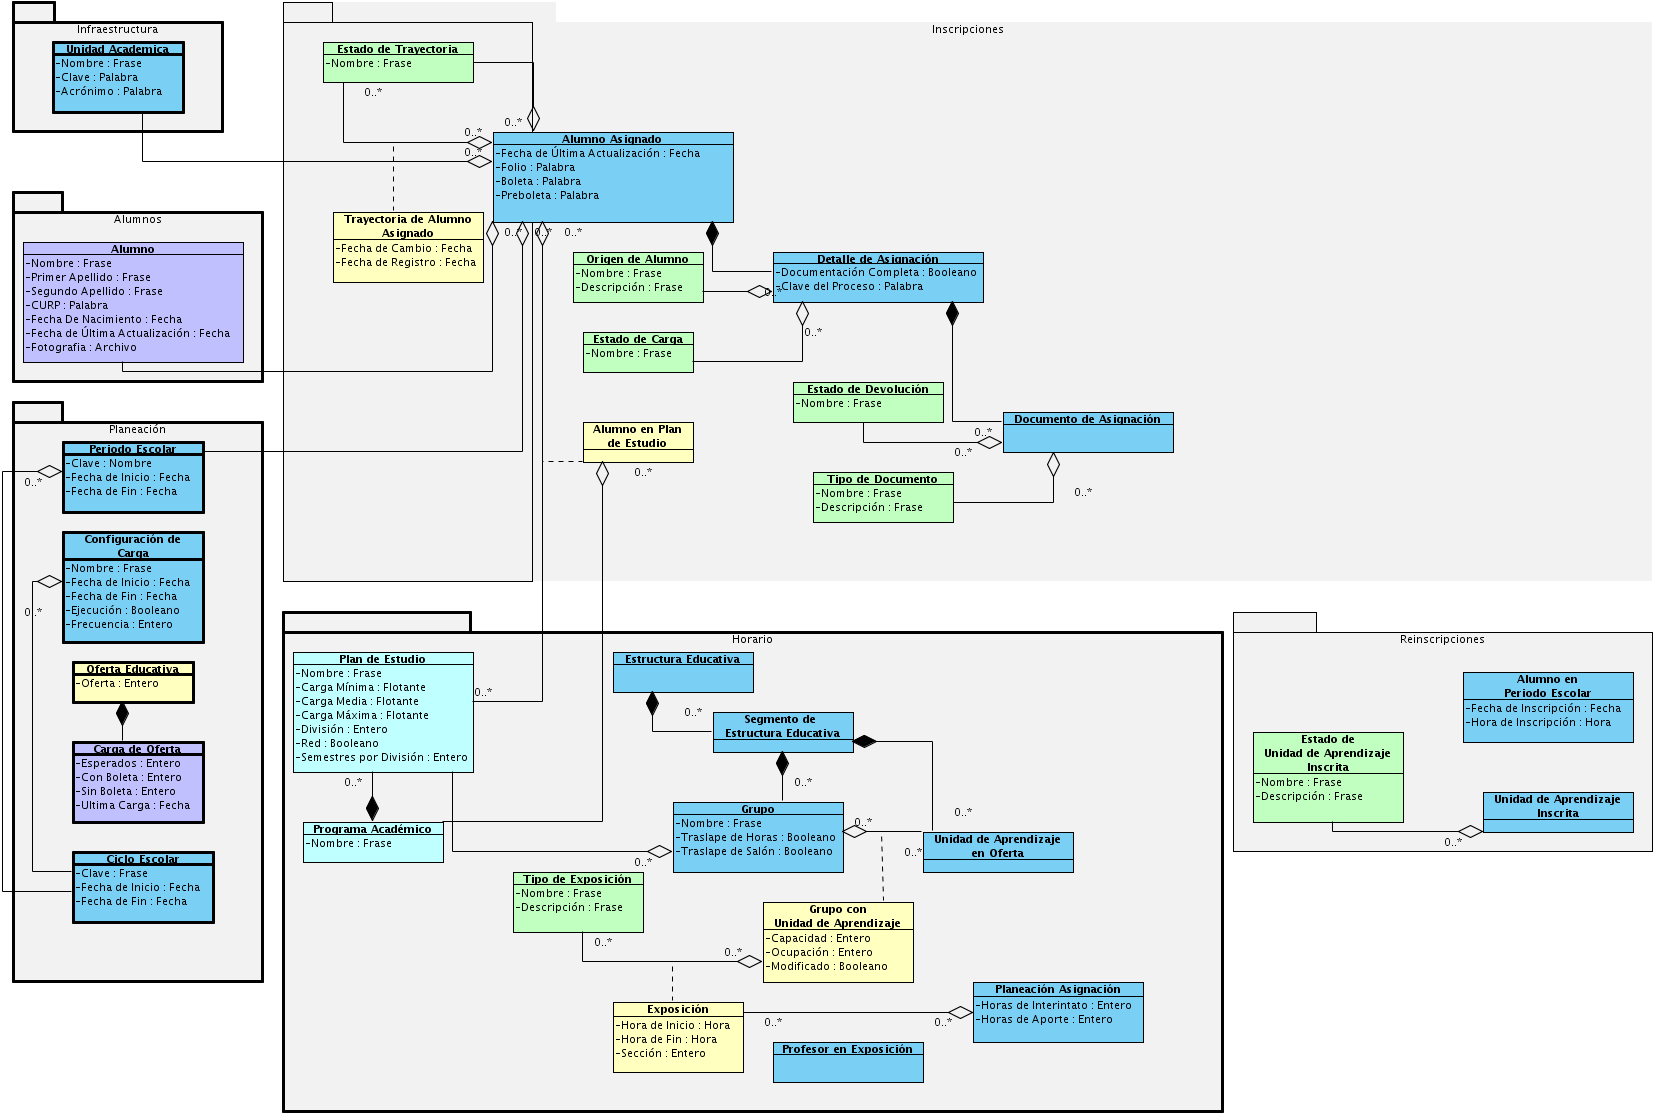
\includegraphics[width=\textwidth]{negocio/images/Inscripciones_MDI}}
		\caption{Modelo de Información de Inscripciones}
		\label{fig:infoInscripciones}
	\end{center}
\end{figure}

\section{Planeación}

	Cada cierto periodo de tiempo en el Instituto se forma una comisión en la que se delibera y establecen los eventos académicos con más relevancia para la comunidad, dando como resultado la estructuración y conformación del Calendario Académico por medio del cual una o varios Unidades Académicas se regirán para la realización de actividades. En este calendario se establecen los periodos de evaluación, los periodos para reinscripciones e inscripciones, los periodos para la aplicación de E.T.S. así como las fechas feriadas.\\

% CICLO ESCOLAR
\begin{cdtEntidad}[Lapso anual que define el Calendario Académico del Instituto Politécnico Nacional.]{CicloEscolar}{Ciclo Escolar}%REGLAMENTO General de Estudios pagina 7
		\brAttr{clave}{Clave}{palabra}{Es el conjunto de caracteres que denotan a un lapso anual en el cual se llevan a cabo actividades administrativas y de docencia.}{\datRequerido}%check
		
	\brAttr{fechaDeInicio}{Fecha de Inicio}{fecha}{Específica el día en el año en que el ciclo escolar da inicio y que sirve como base para la definición del comienzo de sus calendarios académicos. Este dato es relativo a cada Unidad Académica o Calendario Académico.}{\datOpcional}
	
	\brAttr{fechaDeTermino}{Fecha de Término}{fecha}{Específica el día en el año en que el ciclo escolar concluye y que sirve como base para la definición del término de sus calendarios académicos. Este dato es relativo a cada Unidad Académica o Calendario Académico.}{\datOpcional}
	
	\cdtEntityRelSection
	
	\brRel{\brRelComposition}{\refElem{CalendarioAcademico}}{En un Ciclo Escolar se {\bf elaboran} uno o más Calendarios Académicos para coordinar y supervisar las actividades de gestión escolar.}% Reglamento orgánico pag. 34
	
	\brRel{\brRelComposition}{\refElem{PeriodoEscolar}}{En un Ciclo Escolar {\bf se señalan}  dos Periodos Escolares para cursar unidades de aprendizaje.} % Reglamento general de estudios, pag. 8
	
	% TODO: Referenciar a la entidad
	% TODO: ?`Se debe quitar?
	\brRel{\brRelAgregation}{\refElem{UnidadAcademica}}{Una Unidad Académica {\bf opera} durante uno o más Ciclo Escolar y esto es de acuerdo a los programas académicos que ofrece y sus modalidades.}% 

\end{cdtEntidad}

% CALENDARIO ACADÉMICO
\begin{cdtEntidad}[Es la planeación y estructuración que define los tiempos en programación que define se realizan anualmente las actividades académicas y de gestión escolar, en las diversas modalidades educativas que imparte el Instituto.]{CalendarioAcademico}{Calendario Académico}% Reglamento general de estudios pag. 7

	\brAttr{nombre}{Nombre}{frase}{Es la palabra o el conjunto de palabras que denotan e identifican la definición de tiempos para realizar las actividades académicas y de gestión escolar en una o varias Unidades Académicas y para modalidades distintas. }{\datRequerido}

	\cdtEntityRelSection
	
	\brRel{\brRelComposition}{\refElem{CicloEscolar}}{A un Ciclo Escolar se le definen los Calendarios Académicos que sirven para estructurar y conformar los periodos de tiempo en que se llevan a cabo actividades académicas y de gestión.}

	\brRel{\brRelComposition}{\refElem{ActividadCalendario}}{Un Calendario Académico esta {\bf constituido} por un conjunto de tareas académicas y de gestión definidas para llevarse a cabo en un periodo de tiempo el cual debe estar dentro de los limites de un ciclo escolar. }

	% TODO: Referenciar a la entidad
	\brRel{\brRelAgregation}{\refElem{UnidadAcademica}}{Un Calendario Académico {\bf aplica} para un conjunto de Unidades Académicas, las cuales llevarán a cabo sus actividades administrativas y  académicas con base en la planeación definida en el Calendario.}

%	Se eliminará porque es un catálogo
%	\brRel{\brRelAgregation}{\refElem{Modadlidad}}{Una unidad académica se rige por uno o varios calendarios  dependiendo de sus programas académicos y sus modalidades.}
	
	\brRel{\brRelAgregation}{\refElem{CalendarioAcademico}}{Un Calendario Académico puede tener un {\bf Calendario Hijo}, cuando este requiere ser especificado para una Unidad Académica. Y un Calendario Académico puede tener un {\bf Calendario Base} si y solo si ha sido especificado para una Unidad Académcia.}
	
\end{cdtEntidad}

% PERIODO ESCOLAR
\begin{cdtEntidad}[Es el lapso señalado en el Calendario Académico para cursar Unidades de Aprendizaje de un Programa Académico.]{PeriodoEscolar}{Periodo Escolar}% Reglamento general de estudios pag. 8

	\brAttr{clave}{Clave}{frase}{Es el conjunto de caracteres que identifica el lapso de tiempo dentro de un ciclo escolar en el que se cursan Unidades de Aprendizaje definidas por la estructura educativa determinada en un periodo escolar.}{\datRequerido}
	
	\brAttr{fechaInicio}{Fecha de Inicio}{fecha}{Indica el día en el que inicia el lapso de tiempo para cursar Unidades de Aprendizaje de un Programa Académico.}{\datRequerido}
	
	\brAttr{fechaTermino}{Fecha de Término}{fecha}{Indica el día en el que concluye el lapso de tiempo para cursar Unidades de Aprendizaje de un Programa Académico.}{\datRequerido}
	
	\cdtEntityRelSection
	
	\brRel{\brRelComposition}{\refElem{CicloEscolar}}{Un Periodo Escolar es {\bf señalado} dentro de un Ciclo Escola.}

	\brRel{\brRelComposition}{\refElem{ActividadCalendario}}{En un Periodo Escolar {\bf se definen}  las actividades que determinan las acciones que cada Unidad Académica que conforman el Calendario Académico.}

	% Rev. Ulises Vélez: Ok. 
	\brRel{\brRelAgregation}{\refElem{UnidadAcademica}}{En un Periodo Escolar se {\bf ofertan} Programas Académicos por las Unidades Académicas.}
		
\end{cdtEntidad}

%ACTIVIDAD CALENDARIO
\begin{cdtEntidad}[Es una lapso de tiempo en el que una actividad académica debería realizarse.]{ActividadCalendario}{Actividad de Calendario}
	
	\brAttr{fechaInicio}{Fecha de Inicio}{fecha}{Es el día dentro de un Ciclo Escolar en el que se define el comienzo de una Actividad que pertenece al Calendario Académico y que las Unidades Académicas asociadas a ese Calendario deberán comenzar a realizar.}{\datRequerido}
	
	\brAttr{fechaFin}{Fecha de Fin}{fecha}{Es el día dentro de un Ciclo Escolar en el que se define el la conclusión de una Actividad que pertenece al Calendario Académico y que las Unidades Académicas asociadas a ese Calendario deberán finalizar.}{\datRequerido}

	\cdtEntityRelSection
		
	\brRel{\brRelComposition}{\refElem{PeriodoEscolar}}{Una Actividad de Calendario se {\bf realiza} dentro de un Periodo Escolar.}

\end{cdtEntidad}

% CICLO DE UNIDAD ACADÉMICA
\begin{cdtEntidad}[\TODO]{TipoDeActividad}{Tipo de Actividad}
\end{cdtEntidad}

% CALENDARIO DE UNIDAD
\begin{cdtEntidad}[\TODO]{Actividad}{Actividad}
\end{cdtEntidad}

%-------------------------------------Configuración de Proceso de Inscripción--------------------------------------
\section{Configuración de Proceso de Inscripción}

Es el proceso de la importación de los aspirantes de nuevo ingreso, de cambio de carrera o alumno de movilidad cuya información será actualizada e importada al CALMÉCAC.

% PROGRAMA 
\begin{cdtEntidad}[Es la programación del proceso de importación de aspirantes y actualización de información desde el sistema de Admisión.]{Programa}{Programa}

	\brAttr{nombre}{Nombre}{frase}{Identificador de la programación del proceso.}{\datRequerido}

	\brAttr{estado}{Estado}{entero}{Indica el estado en el que se encuentra el proceso: En ejecución o detenido.}{\datRequerido}

	\brAttr{fechaInicio}{Fecha de Inicio}{fecha}{Indica la fecha y hora en la que el proceso debe empezar a ejecutarse periódicamente de acuerdo a la Frecuencia de Ejecución.}{\datRequerido}
	
	\brAttr{fechaTermino}{Fecha de Término}{fecha}{Indica la fecha y hora en la que el proceso debe dejar de ejecutarse periódicamente.}{\datRequerido}
	
	\brAttr{confirmacionAutomatica}{Confirmación Automática}{boleano}{Indica el valor del atributo ``confirmado'' que debe tener por defecto un Aspirante al ser importad. Por defecto es ``verdadero''. No se usa.}{\datRequerido}
	
	\brAttr{frecuenciaDeEjecucion}{Frecuencia de Ejecución}{entero}{Indica la frecuencia con que debe ejecutarse el proceso, indicando la cantidad como un valor entero y la unidad de medida de esta cantidad corresponde a la ``Parte Fecha''.}{\datRequerido}
	
	\cdtEntityRelSection
	
	\brRel{\brRelComposition}{\refElem{Parte Fecha}}{Un Programa se {\bf ejecuta} cada cierto tiempo (indicado en Frecuencia de Ejecución) expresado en {\bf Parte Fecha}.}
	\brRel{\brRelComposition}{\refElem{Corrida}}{La ejecución de un Programa {\bf se registra en} una Corrida.}

\end{cdtEntidad}

% CORRIDA
\begin{cdtEntidad}[Es el registro de la ejecución del proceso de inscripción]{Corrida}{Corrida}

	\brAttr{duracion}{Duración}{hora}{Indica el tiempo medido en milisegundos transcurrido durante la ejecución del proceso.}{\datRequerido}
	
	\brAttr{fechaDeEjecucion}{Fecha de Ejecución}{fecha}{Día y hora en el que el proceso de inscripción inició su ejecución.}{\datRequerido}
	
	\brAttr{resultado}{Resultado}{frase}{Texto que indica el resultado de la ejecución. Debe indicar que la ejecución fue correcta o describir textualmente las fallas que se encontraron durante la ejecución.}{\datRequerido}
	
	\cdtEntityRelSection
	
	\brRel{\brRelComposition}{\refElem{Programa}}{Una Corrida {\bf registra} la ejecución de un Programa.}
	
\end{cdtEntidad}

%-------------------------------------Infraestructura--------------------------------------
\section{Infraestructura}

\TODO

% Unidad Académica
\begin{cdtEntidad}[\TODO]{UnidadAcademica}{Unidad Académica}

	\brAttr{nombre}{Nombre}{frase}{Es la palabra o el conjunto de palabras que denotan e identifican a la Unidad Académica.}{\datRequerido}

	\brAttr{clave}{Clave}{frase}{Es el conjunto de caracteres que identifica a la Unidad Académica en el Instituto.}{\datRequerido}

	\brAttr{acronimo}{Acrónimo}{palabra}{Palabra formada por las iniciales de la Unidad Académica que la identifican en el Instituto.}{\datRequerido}
		
	\cdtEntityRelSection
	
	\brRel{\brRelAgregation}{\refElem{PeriodoEscolar}}{\TODO}
	
	\brRel{\brRelAgregation}{\refElem{CicloEscolar}}{\TODO}
	
	\brRel{\brRelAgregation}{\refElem{CalendarioAcademico}}{\TODO}
	
\end{cdtEntidad}

%%%%%%%%%%%%%%%%%%%%%Horarios
\section{Horarios}

Una Unidad Académica realiza semestralmente la planeación relacionada a la distribución de Unidades de Aprendizaje en espacios y horarios, así como de asignación de Profesores que realizaran las exposiciones para el periodo definido por la Estructura Educativa. En el caso de los profesores cuya relación con el Instituto se define por un contrato se requerirá la justificación que soporte la falta de horas frente a grupo. A toda esta planeación se le conoce como Estructura Educativa y es uno de los procesos más grandes y complejos del Instituto, ya que requiere de la más alta cooperación entre las distintas áreas internas y externas de una Unidad Académica.\\

En el paquete de \textit{Horarios} se verán reflejadas las relaciones entre las entidades que permiten ejecutar está operación y cómo se almacenarán en el sistema para su consulta y edición.\\

\begin{cdtEntidad}[Es la entidad que integra todos los planes de estudios ofertados por las Unidades Académicas del Instituto.]{PlanDeEstudio}{Plan de Estudio}

	\brAttr{cargaMinima}{Carga Mínima de Créditos}{flotante}{Es un dígito que representa el cálculo obtenido de dividir el número total de créditos del programa académico entre el número de periodos escolares de la duración máxima del plan de estudio.}{\datOpcional}
	
	\brAttr{cargaMedia}{Carga Media de Créditos}{flotante}{Es un dígito que representa el cálculo obtenido de al dividir el número total de créditos del programa académico entre el número de periodos escolares de la duración máxima del plan de estudio}{\datOpcional}
	
	\brAttr{cargaMaxima}{Carga Máxima de Créditos}{flotante}{Es un dígito que representa el cálculo obtenido de dividir  el número total de créditos del programa académico entre el número de periodos escolares de la duración mínima del plan de estudio.}{\datOpcional}
	
	\brAttr{division}{División}{entero}{Es un dígito que representa el número segmentaciones que un Plan de Estudios tiene para ubicar sus Unidades de Aprendizaje.}{\datRequerido}
	
	\brAttr{red}{Red}{entero}{Indica si el Plan de Estudio es compartido e impartido entre distintas Unidades Académicas.}{\datOpcional}
	
	\brAttr{planDeEstudio}{Plan de Estudio}{frase}{Es la palabra o conjunto de palabras que representan e identifica a la estructura curricular derivada de un Programa Académico.}{\datOpcional}
	
	
	\cdtEntityRelSection
	
	\brRel{\brRelAgregation}{\refElem{PeriodoEnUnidadAcademica}}{El plan de estudio de un programa académico es ofertado en una unidad académica durante uno o más periodos escolares.}
	
\end{cdtEntidad}

\section{Inscripciones}

\begin{cdtEntidad}[Son los Programas Académicos que oferta cada Unidad Académica en Cada Periodo Escolar.]{PeriodoEnUnidadAcademica}{Periodo en Unidad Académica}

	\brAttr{fechaInicio}{Fecha de Inicio}{fecha}{Indica el día en que inicia la oferta de un démico en un Periodo Escolar y Unidad Académica.}{\datRequerido}
	
	\brAttr{fechaTermino}{Fecha de Término}{fecha}{Indica el día en que concluye la oferta de un Programa Académico en un Periodo Escolar y Unidad Académica.}{\datRequerido}
	
	\cdtEntityRelSection
	
	\brRel{\brRelComposition}{\refElem{PlanDeEstudio}}{Un Periodo en Unidad Académica {\em especifica una oferta} de un Plan de Estudios.}
	\brRel{\brRelComposition}{\refElem{UnidadAcademica}}{Un Periodo en Unidad Académica {\em especifica una oferta} en una Unidad Académica}
	\brRel{\brRelComposition}{\refElem{PeriodoEscolar}}{Un Periodo en Unidad Académica {\em especifica una oferta} en un Periodo Escolar.}
\end{cdtEntidad}


%\TODO: En el MDI cambiar Plan de Estudios por Plan de Estudio
\begin{cdtEntidad}[Agrupa y los ingresos de Aspirantes a Planes de Estudios de Unidades Académicas por Tipo de Carga]{PlanDeEstudioEnPeriodoDeUnidadAcademica}{Plan de Estudio en Periodo de Unidad Académica}
	
	\brAttr{oferta}{Oferta}{entero}{Es el número de estudiantes esperados (lugares disponibles) para inscribir Alumnos de nuevo ingreso a un Plan de Estudio Ofertado en un Periodo Escolar.}{\datRequerido}
	
	\brAttr{estudiantesEsperados}{Estudiantes Esperados}{entero}{Es el número de estudiantes esperados (lugares disponibles) para inscribir Alumnos de nuevo ingreso a un Plan de Estudio Ofertado en un Periodo Escolar.}{\datRequerido}
	
	\brAttr{estudiantesCargadosConBoleta}{Estudiantes Cargados con Boleta}{entero}{Es el número de alumnos de nuevo ingreso que {\bf cuentan} con número de Boleta para el Plan de Estudios, Unidad Académica y Periodo Escolar correspondiente y que {\bf no han sido inscritos}.}{\datRequerido}
	
	\brAttr{estudiantesCargadosSinBoleta}{Estudiantes Cargados sin Boleta}{entero}{Es el número de alumnos de nuevo ingreso que {\bf no cuentan} con número de Boleta para el Plan de Estudios, Unidad Académica y Periodo Escolar correspondiente y que {\bf no han sido inscritos}.}{\datRequerido}
	
	\brAttr{estudiantesInscritosSinBoleta}{Estudiantes Inscritos sin Boleta}{entero}{Es el número de alumnos de nuevo ingreso que {\bf no cuentan} con número de Boleta para el Plan de Estudios, Unidad Académica y Periodo Escolar correspondiente y que {\bf ya han sido inscritos}.}{\datRequerido}
	
	\brAttr{estudiantesInscritosConBoleta}{Estudiantes Inscritos con Boleta}{entero}{Es el número de alumnos de nuevo ingreso que {\bf cuentan} con número de Boleta para el Plan de Estudios, Unidad Académica y Periodo Escolar correspondiente y que {\bf ya han sido inscritos}.}{\datRequerido}
	
	\brAttr{estudiantesCancelados}{Estudiantes Cancelados}{entero}{Es el número de alumnos de nuevo ingreso cuyo ingreso al IPN se encuentra en proces de cancelación por los motivos establecidos en el \textbf{Artículo 14} del \textbf{Reglamento General de Estudios}.}{\datRequerido}
	
	\brAttr{fechaDeUltimaActualizacion}{Fecha de Última Actualización}{fecha}{Indica el día y la hora en que esta información ha sido modificada por última vez.}{\datOpcional}
	% TODO: Debería ser ``Convocatoria''.
	\brAttr{tipoDeCarga}{Tipo de Carga}{TipoDeCarga}{Indica el tipo de carga realizado.}{\datRequerido}
	
	\cdtEntityRelSection
	
	\brRel{\brRelComposition}{\refElem{AlumnoAsignado}}{A un Plan de Estudio en Periodo de Unidad Académica {\bf se le asignan} Alumnos Asignados.}
	
\end{cdtEntidad}


\begin{cdtEntidad}[Es un aspirante o alumno que al haber aprobado el examen de Admisión y que cumple con los requisitos de la convocatoria correspondiente es asignado a un plan de estudio ofertado por una Unidad Académica en un periodo escolar. Tiene como propósito especificar si el aspirante tiene la documentación requerida para completar el proceso de Inscripción o si requiere realizar una corrección o si su asignación debe ser anulada.]{AlumnoAsignado}{Alumno Asignado}

	\brAttr{observacionesDeDocumentacion}{Observaciones de Documentación}{texto}{Especifica las observaciones del personal de Gestión Escolar en caso de que no haya sido satisfactoria la entrega de documentos a un Aspirante una vez que haya completado su Inscripción y se le haya asignado su número de Boleta.}{\datOpcional}
	
	\brAttr{folio}{Folio}{palabra}{Identificador del aspirante junto con Clave en el proceso, utilizado únicamente durante el proceso de admisión.}{\datRequerido}
	
	\brAttr{claveEnElProceso}{Clave del Proceso}{palabra}{Indica el proceso mediante el cual el aspirante fue asignado: Convocatoria de nuevo ingreso, movilidad, cambio de carrera, RVOE, etc.}{\datRequerido}
	
	\brAttr{preboleta}{Preboleta}{palabra}{Identificador del estudiante mientras no cuente con Boleta. Permite identificar el tipo u origen del alumno.}{\datOpcional}
	
	\brAttr{boleta}{Boleta}{palabra}{Identificador del Alumno dentro del Instituto. Su asignación le permite tener todos los derechos como estudiante. Al no contar con Boleta al estudiante se le denomina Aspirante.}{\datOpcional}
	
	\brAttr{fechaDeUltimaCarga}{Fecha de Última Carga}{fecha}{Indica fecha y hora de la última  actualización la información.}{\datOpcional}
	
	\brAttr{estadoDeCargaDelAlumno}{Estado de Carga del Alumno}{EstadoDeCargaDelAlumno}{Indica la condición en la que se encuentra un Aspirante después de que se realiza una carga en el sistema de la información de su documentación o de su asignación de boleta o preboleta.}{\datRequerido}
	
	\brAttr{estadoDeDocumentacion}{Estado de Documentación}{EstadoDeDocumentacion}{Indica si a un Alumno Asignado con Boleta se le ha entregado la documentación o si dicha entrega tiene observaciones.}{\datRequerido}
		
	\brAttr{estadoDelAlumno}{Estado del Alumno}{EstadoDelAlumno}{Indica el estado en el que se encuentra el Alumno.}{\datRequerido}
	
	\cdtEntityRelSection
	
	\brRel{\brRelAgregation}{\refElem{Documento}}{A un Alumno Asignado se le {\bf entregan} Documentos.}
	
	\brRel{\brRelComposition}{\refElem{SituacionEscolar}}{Un Alumno Asignado {\bf tiene} una Situación Escolar.}
	
	\brRel{\brRelComposition}{\refElem{Alumno}}{Un Alumno Asignado {\bf es} un Alumno.}


\end{cdtEntidad}


\begin{cdtEntidad}[\TOCHK Es la condición que un Alumno Asignado tiene en un Plan de Estudios. Indica algunas propiedades que permiten efectuar operaciones en el sistema de parte del Alumno así como de otros procesos que lo involucren.]{SituacionEscolar}{Situación Escolar}

	\brAttr{promedioGeneral}{Promedio General}{flotante}{Es el número que indica resultado de efectuar la suma de las calificaciones obtenidas de las Unidades de Aprendizaje Cursadas entre el número de Unidades de Aprendizaje Cursadas.}{\datOpcional}
	
	\brAttr{creditosObtenidos}{Créditos Obtenidos}{flotante}{Es el número que indica el resultado de efectuar la suma de los créditos S.A.T.C.A. de las Unidades de Aprendizaje Cursadas y cuya calificación es mayor a la mínima aprobatoria de acuerdo al \textbf{Artículo 40} del \textbf{Reglamento General de Estudios}. Tiene como propósito ser uno de los mecanismos que indiquen el grado de avance del Alumno en el plan de estudio.}{\datOpcional}
	
	\brAttr{creditosFaltantes}{Créditos Faltantes}{flotante}{Es el número que indica el resultado de efectuar la resta de los créditos totales de un plan de estudios con los obtenidos por el Alumno. Tiene como propósito ser uno de los mecanismos que indiquen el grado de avance del Alumno en el plan de estudio. }{\datOpcional}
	
	\brAttr{uDeAAprobadas}{Unidades de Aprendizaje Aprobadas}{entero}{Es el número que indica la cantidad de Unidades de Aprendizaje de un plan de estudio que un Alumno ha acreditado.}{\datOpcional}
	
	\brAttr{uDeAReprobadas}{Unidades de Aprendizaje Reprobadas}{entero}{Es el número que indica la cantidad de Unidades de Aprendizaje de un plan de estudio que no ha acreditado.}{\datOpcional}
	
	\brAttr{uDeADesfasadas}{Unidades de Aprendizaje Desfasadas}{entero}{Es el número que indica las unidades de aprendizaje que entran en el siguiente criterio: ´´\textit{Ningún alumno podrá cursar asignaturas o equivalentes que correspondan a más de tres periodos escolares consecutivos y no podrá adeudar las correspondientes de más de dos periodos escolares previos al que curse.}''}{\datOpcional}
	
	\brAttr{semestreActual}{Semestre Actual}{entero}{\TOCHK Es el número que indica el semestre en el que se encuentra un Alumno con base en el plan de estudio y las Unidades de Aprendizaje inscritas en el periodo corriente. }{\datOpcional}
	
	\brAttr{periodosTranscurridos}{Periodos Transcurridos}{entero}{\TOCHK Es el número que indica la cantidad de periodos en los que un alumno ha inscrito Unidades de Aprendizaje.}{\datOpcional}
	
	\brAttr{periodosDeBajaTemporal}{Periodos de Baja Temporal}{entero}{\TOCHK Es el número que indica la cantidad de periodos en los que un Alumno no ha efectuado una reinscripción pero cuya justificación se encuentra apoyada por un documento aprobado por el Director de la Unidad Académica a la cual el Alumno fue asignado.}{\datOpcional}
	
	\brAttr{porcentajeDeCreditos}{Porcentaje de Créditos}{flotante}{\TOCHK Es un número que representa el resultado de efectuar la suma de los créditos S.A.T.C.A. obtenidos entre el total de las Unidades de Aprendizaje del plan de estudio. }{\datOpcional}
	
	\brAttr{periodosEstimados}{Periodos Estimados}{entero}{\TODO}{\datOpcional}
	
\end{cdtEntidad}


\begin{cdtEntidad}[Es el resultado de la relación de \refElem{tdDocumento} y \refElem{AlumnoAsignado} y tiene como propósito almacenar todos los documentos que son requeridos para el proceso de Inscripción del Instituto y que fueron entregados por el Aspirante.]{DocumentoDeAlumnoAsignado}{Documento de Alumno Asignado}

	\brAttr{estadoDevolucionDocumento}{Estado de Devolución de Documento}{EstadoDeDevolucionDeDocumento}{Indica la condición que presenta un documento entregado por un Aspirante y tiene como propósito definir si el documento ha sido entregado de forma satisfactoria o si requiere de una corrección.}{\datRequerido}

\end{cdtEntidad}
        
        
        %---------- Modelo de información de EE ----------
	    \chapter{Modelo de Información de EE}
	    \label{ch:ee}
	    \begin{cdtEntidad}[Es el proceso mediante el cual el Responsable de Estructura Educativa de una Unidad Académica asigna espacios,horarios y profesores a las Unidades de Aprendizaje que se ofertarán para un periodo. También se puede ver como una entidad que almacenará toda esa información así como toda la bitácora de control de parte de la DGyCE ,que es el órgano que tiene como tarea vigilar que cada uno de los profesores, cuya relación con el Instituto esta definida por un contrato, estén cumpliendo su carga máxima de horas.]{EstructuraEducativa}{Estructura Educativa}
	
	\brAttr{estadoDeEstructuraEducativa}{Estado de Estructura Educativa}{EstadoDeEstructuraEducativa}{Indica la situación de la estructura educativa que define si es editable o no y de esta forma establecer sus procesos aplicables.}{\datRequerido}
	
	\cdtEntityRelSection
	
	\brRel{\brRelComposition}{\refElem{SegmentoDeEstructuraEducativa}}{Una Estructura Educativa se encuentra compuesta por segmentos(grupos que implican horarios,  profesores, espacios y el soporte documental que justifica la falta de horas frente a grupo de un profesor) que requieren su aprobación o corrección de acuerdo a su contenido.}
	
	\brRel{\brRelComposition}{\refElem{tUnidadAcademica}}{Cada periodo el Responsable de la Estructura Educativa de una Unidad Académica planea y  crea la Estructura Educativa que mejor se ajuste a la demanda de Unidades de Aprendizaje y al número de alumnos(matrícula) que se estima se inscribirán en un periodo.  }
	
		\brRel{\brRelAgregation}{\refElem{PeriodoEscolar}}{Para un periodo escolar se definen:
			\begin{Citemize}
				\item Unidades de Aprendizaje a Ofertar las cuales vienen de un Plan de Estudio.
				\item Días en los que se llevarán a cabo actividades académicas y de administración.
				\item Grupo junto con su asignación de espacios, horarios y profesores.
			\end{Citemize} 
			En conjunto está información compone a una Estructura Educativa.}

\end{cdtEntidad}

\begin{cdtEntidad}[Una Estructura Educativa está conformada por conjuntos de elementos en los que, de acuerdo a la modalidad de los programas académicos y/o a los planes de estudio que en una Unidad Académica se ofertan, se requiere realizar la definición de las Unidades de Aprendizaje a ofertar en adición a su asignación de espacios en donde se realizará la exposición de  de sus contenidos, la asignación los profesores que realizarán estas exposiciones,sus horarios y los espacios en los que se llevarán a cabo. Estos elementos son revisados por los analistas de la DGyCE.]{SegmentoDeEstructuraEducativa}{Segmento de Estructura Educativa}

	\brAttr{estadoDeSegmentoDeEstructuraEducativa}{Estado de Segmento de Estructura Educativa}{EstadoDeEstructuraEducativa}{Indica la situación en la que se encuentra el segmento de la estructura educativa y de esta forma definir si es editable o no y establecer sus procesos aplicables.}{\datRequerido}
	
	\brAttr{nivelAcademico}{Nivel Académico}{NivelAcademico}{Indica para cuál de los niveles ofertados en la unidad académica se crea el segmento de la estructura educativa.}{\datRequerido}
	
	\brAttr{modalidad}{Modalidad}{Modalidad}{Indica para cuál de las distintas modalidades que se ofrecen en el Instituto y están definidos en los programas académicos en una unidad académica se crea el segmento de estructura educativa.}{\datRequerido}
	
	 \brAttr{dia}{Día}{dia}{Es el conjunto de días de la semana en los que una Unidad Académica labora para un Segmento de Estructura Educativa.}
	{\datRequerido}
	
	\brAttr{turno}{Turno}{Turno}{El Responsable de Estructura Educativa de una Unidad Académica definirá la hora de inicio y la hora de término de los que turnos que se aplicarán para los días laborales de un Segmento de Estructura Educativa. }{\datRequerido}
	 \cdtEntityRelSection
	 %AQUIII
	 \brRel{\brRelComposition}{\refElem{EstructuraEducativa}}{Una Estructura Educativa se encuentra compuesta por segmentos(grupos que implican horarios,  profesores, espacios y el soporte documental que justifica la falta de horas frente a grupo de un profesor) que requieren su aprobación o corrección de acuerdo a su contenido.}
	 
	 
	 \brRel{\brRelComposition}{\refElem{UdeAEnOferta}}{Para un Segmento de Estructura Educativa se seleccionarán las Unidades de Aprendizaje de un plan de estudio que correspondan con la modalidad y el nivel académico del Segmento, las cuales  se ofrecerán para un periodo de acuerdo a la plantilla estudiantil y a el historial generado por  Estructuras Educativas previas.}
	 
	\brRel{\brRelComposition}{\refElem{Grupo}}{Para un segmento de Estructura Educativa se definen los  grupos en los que se realizará la exposición de los contenidos de las Unidades de Aprendizaje que se seleccionaron para su oferta.}
	 
	\brRel{\brRelComposition}{\refElem{ProfesorEnSegmento}}{Un segmento de estructura educativa está compuesto por los profesores asignados para la exposición de contenidos de las Unidades de Aprendizaje o la realización de Actividades Complementarias.}
	 
\end{cdtEntidad}
 
 
 \begin{cdtEntidad}[Un grupo es un mecanismo el cual esta constituido por  un cierto número de Unidades de Aprendizaje, pertenecientes a un Plan de Estudio que se ofertará para un periodo, los horarios y días de la semana en que sus contenidos deberán ser expuestos a una agrupación de alumnos.]{Grupo}{Grupo}
 
 	\brAttr{nombre}{Nombre del Grupo}{frase}{Es el conjunto de caracteres que definen e identifican a una agrupación de Unidades de Aprendizaje junto con su asignación de horarios y profesores en un Segmento de Estructura Educativa. Por ejemplo: 
 	\begin{itemize}
 		\item 1CM1
 		\item 4CV2
 	\end{itemize}}{\datRequerido}
 	
 	\brAttr{traslapeDeHorario}{Traslape de Horario}{booleano}{Especifica que es posible que en el grupo se pueden impartir unidades de aprendizaje al mismo tiempo o cubriendo tiempo una de otra.}{\datRequerido}
 	
 	\brAttr{traslapeDeSalon}{Traslape de Salón}{booleano}{Especifica que es posible que en el grupo se puedan impartir unidades de aprendizaje en el mismo espacio. }{\datRequerido}
 	
	\cdtEntityRelSection
	
	 \brRel{\brRelComposition}{\refElem{SegmentoDeEstructuraEducativa}}{Para un segmento de Estructura Educativa se definen los  grupos en los que se realizará la exposición de los contenidos de las Unidades de Aprendizaje que se seleccionaron para su oferta.}
	 
	 \brRel{\brRelAgregation}{\refElem{TurnoEnSegmento}}{A un grupo se le asigna el segmento de horas en el día en que se realizará la exposición del contenido de las Unidades de Aprendizaje que le fueron definidas.}
	 
	 \brRel{\brRelAgregation}{\refElem{UdeAEnOferta}}{A un grupo se le asignan un subconjunto de las Unidades de Aprendizaje en Oferta para que se realice la exposición de su contenido durante un periodo.}
	 
\end{cdtEntidad}
 
\begin{cdtEntidad}[Es un Profesor que se encuentra dentro de uno o más segmentos de una Estructura Educativa porque se le han definido Actividades Complementarias que realizar durante un periodo y/o esta asignado para realizar la Exposición de los contenidos de varias Unidades de Aprendizaje Ofertadas.]{ProfesorEnSegmento}{Profesor en Segmento}

	\brAttr{numeroDeHoras}{Número de Horas}{flotante}{Es el dígito que representa el número de horas totales a las que un profesor esta asignado dentro de un Segmento de Estructura Educativa.}{\datRequerido}
	
	\brAttr{horasDeInterinato}{Horas de Interinato}{flotante}{Es el dígito que representa el número de horas totales de interinato a las que un profesor está asignado dentro de un Segmento de Estructura Educativa. }{\datOpcional}
 	
 	\brAttr{horaDeAporte}{Horas de Aporte}{flotante}{Es el dígito que representa el número de horas totales a las que un profesor esta asignado dentro de un Segmento de Estructura Educativa y por las cuales no se le paga.}{\datOpcional}
 
 	\brAttr{actividadComplementaria}{Actividad Complementaria}{ActividadComplementaria}{Es el conjunto de actividades que un profesor del Instituto realiza con el fin de reponer aquellas horas que no pudieron ser asignadas frente a grupo.}{\datRequerido}
 	
 	\cdtEntityRelSection
 	
 	\brRel{\brRelAgregation}{\refElem{Profesor}}{Un profesor es adherido a un Segmento de Estructura Educativa cuando se le asignan  una o más actividades complementarias a realizar o horas para la exposición de contenidos de las Unidades de Aprendizaje.}
 	
 	\brRel{\brRelComposition}{\refElem{SegmentoDeEstructuraEducativa}}{Un segmento de estructura educativa esta compuesto por los profesores asignados para la exposición de contenidos de las Unidades de Aprendizaje o la realización de Actividades Complementarias.}
 	
 	\brRel{\brRelComposition}{\refElem{PlaneacionAsignacion}}{Un profesor se encuentra dentro de un Segmento de Estructura Educativa cuando ha sido asignado para realizar la exposición }
 
 \end{cdtEntidad}
 
 \begin{cdtEntidad}[Es la entidad que representa a una Unidad de Aprendizaje de un Plan de Estudios que fue seleccionada para ofertarse en el periodo para el cual se elabora la Estructura Educativa .Estas Unidades de Aprendizaje son seleccionadas con base en la plantilla estudiantil y al historial de Estructuras Educativa previas y pertenecen a un  Segmento de Estructura Educativa.]{UdeAEnOferta}{Unidad de Aprendizaje en Oferta}
 	
 	\cdtEntityRelSection
 	
 	\brRel{\brRelAgregation}{\refElem{Grupo}}{A un grupo se le asignan un subconjunto de las Unidades de Aprendizaje en Oferta para que se realice la exposición de su contenido durante un periodo.}
 	
 	\brRel{\brRelAgregation}{\refElem{UdeA}}{Una de Unidad de Aprendizaje en Oferta adquiere la información de la Unidad de Aprendizaje del Plan de Estudios que pertenece al Segmento de la Estructura Educativa. }
 	
 	 \brRel{\brRelComposition}{\refElem{SegmentoDeEstructuraEducativa}}{Para un segmento de Estructura Educativa se seleccionarán las Unidades de Aprendizaje de los distintos planes de estudio,que correspondan con la modalidad y el nivel académico, que se ofrecerán para un periodo de acuerdo a la demanda y plantilla estudiantil de la Unidad Académica.}
 	 
 	 \brRel{\brRelComposition}{\refElem{Periodo}}{Una Unidad de Aprendizaje es ofertada en un lapo de tiempo durante la ejecución de un periodo escolar.}
 	 
 \end{cdtEntidad}
 
 
 \begin{cdtEntidad}[Es un lapso de tiempo en el que los contenidos de una Unidad de Aprendizaje Ofertada se debe impartir. Este lapso debe encontrarse dentro del rango del Periodo Escolar del cual se esta generando la Estructura Educativa.]{Periodo}{Periodo}
 
 	\brAttr{fechaDeInicio}{Fecha de Inicio}{fecha}{Indica el día dentro de un Periodo Escolar en que se comienzan a impatir los contenidos de una Unidad de Aprendizaje en Oferta.}{\datOpcional}
 	
 	\brAttr{fechaDeFin}{Fecha de Fin}{fecha}{Indica el día dentro de un Periodo Escolar en que se concluye de impartir los contenidos de una Unidad de Aprendizaje en Oferta.}{\datOpcional}
 	
 	\cdtEntityRelSection
 	
 	\brRel{\brRelComposition}{\refElem{UdeAEnOferta}}{Una Unidad de Aprendizaje es ofertada en un lapo de tiempo durante la ejecución de un periodo escolar.}
 
\end{cdtEntidad}
  
 \begin{cdtEntidad}[Es el conjunto de Unidades Temáticas que conforman el contenido de Unidad de Aprendizaje y que se seleccionan para formar parte de un Segmento de la Estructura Educativa ]{SubUdeA}{Sub Unidad de Aprendizaje}
 
 	\brAttr{horas}{Horas}{horas}{Es el conjunto de horas que determinan cuánto tiempo se le dedicará a exponer los contenidos de la Sub Unidad de Aprendizaje.}{\datOpcional}
 
 	\brAttr{profesores}{Profesores}{entero}{Es un dígito que representa la cantidad mínima de profesores que deben cubrir las exposiciones para una Sub Unidad de Aprendizaje.}{\datOpcional}
 	
 	\brAttr{clave}{Clave}{texto}{Conjunto de palabras que identifican a una Sub Unidad de Aprendizaje.}{\datOpcional}
 	
 	\brAttr{tipoUnidadAprendizaje}{Tipo de Unidad de Aprendizaje}{TipodeUdeA}{Indica si los contenidos de una Unidad de Aprendizaje que conforman a la sub unidad son obligatorios y si deben ser aprobados en su totalidad o no.}{\datRequerido}
 	\cdtEntityRelSection
 	
 	\brRel{\brRelComposition}{\refElem{UdeA}}{Una unidad de aprendizaje está compuesta por unidades temáticas y que para un periodo son seleccionables generando una Sub Unidad de Aprendizaje a la que los alumnos se inscriben, si todo el contenido de la unidad de aprendizaje es aprobado, la Unidad de aprendizaje se aprueba directamente, por otro en cambio si se reprueba al menos un contenido, la Unidad de Aprendizaje se dará por reprobada.}
 	
 	\brRel{\brRelAgregation}{\refElem{Exposicion}}{Para una sub unidad de aprendizaje se requiere definir los días de la semana en que se realizaran las exposiciones para que un Profesor transmita su contenido a un grupo de alumnos.}
 \end{cdtEntidad}
 
%% GrupoconUdeA
\begin{cdtEntidad}[Es un periodo de tiempo destinado a la tranmisión de conocimientos de parte de un docente hacía a un conjunto de alumnos inscritos a una unidad de aprendizaje de un grupo.]{Exposicion}{Exposición}
 	
 	\brAttr{horaDeInicio}{Hora de Inicio}{hora}{Indica la hora en un día laboral en que inicia la exposición de los contenidos de  la Unidad de Aprendizaje asignada a un grupo.}{\datRequerido}
 	
 	\brAttr{horaDeTermino}{Hora de Término}{hora}{Indica la hora en un día laboral en que concluye la exposición de los contenidos de  la Unidad de Aprendizaje asignada a un grupo.}{\datRequerido}
 	
 	\brAttr{tipoDeExposicion}{Tipo de Exposición}{TipoDeExposicion}{Indica la forma en que la transmisión de conocimientos se llevará a cabo por parte de el o los profesores asignados a la Unidad de Aprendizaje.}{\datRequerido}
 	
 	\brAttr{seccion}{Sección}{entero}{Es un dígito que representa el número de veces que una Exposición será dividida para impartir los contenidos de la Unidad de Aprendizaje en diferentes espacios. }{\datOpcional}
 	
 	\cdtEntityRelSection
 	
 	\brRel{\brRelAgregation}{\refElem{SubUdeA}}{Para una sub unidad de aprendizaje se requiere definir los días de la semana en que se realizaran las exposiciones para que un Profesor transmita su contenido a un grupo de alumnos.}
 	
 	\brRel{\brRelComposition}{\refElem{GrupoConUdeAEnOferta}}{Para una Unidad de Aprendizaje que se encuentra en un grupo, se requieren definir las distintas exposiciones en las que uno o varios profesores transmitirán los contenidos a una agrupación de alumnos .}
 	
 	\brRel{\brRelAgregation}{\refElem{DiaLaboral}}{La exposición de una Unidad de Aprendizaje o de una Sub Unidad debe llevarse a cabo en uno de los días establecidos como laborales de la Estructura Educativa de una Unidad Académica.}
 	
 	\brRel{\brRelComposition}{\refElem{Seccion}}{Es la división que una exposición puede adquirir a raíz de las necesidades de un grupo dado el número de alumnos que lo conforman y la infraestructura de una Unidad Académica.}

	\brRel{\brRelAgregation}{\refElem{EspacioAsignado}}{Una Exposición requiere impartirse en alguno de los espacios con los que una Unidad Académica cuenta pudiendo ser externos o internos.}
	
	\brRel{\brRelAgregation}{\refElem{PlaneacionAsignacion}}{Un profesor que se encuentra dentro de un Segmento de Estructura Educativa es asignado a más de una exposición de contenido de las Unidades de Aprendizaje asignadas a grupos.}
	

\end{cdtEntidad}

\begin{cdtEntidad}[Tiene como objetivo permitir la exposición de los contenidos de una Unidad de Aprendizaje Ofertada en diferentes horarios y espacios a un subconjunto de alumnos inscritos a un grupo.  ]{Seccion}{Sección}

	\brAttr{capacidad}{Capacidad}{entero}{Es el dígito que representa el número de Alumnos que podrán ingresar a la Sección de una Exposición.}{\datOpcional}

	\cdtEntityRelSection
	
	\brRel{\brRelComposition}{\refElem{Exposicion}}{Es la división que una exposición puede adquirir a raíz de las necesidades un grupo dada la infraestructura de una Unidad Académica y el número de alumnos que conforman a un grupo. }
	
	\brRel{\brRelAgregation}{\refElem{EspacioParaExposicion}}{Para una sección se requiere definir un espacio(de los determinados para la Exposición de una Unidad de Aprendizaje asignada a un grupo)  donde se impartirá el contenido de una Unidad de Aprendizaje.}

\end{cdtEntidad}


\begin{cdtEntidad}[Es el resultado de la relación entre Planeación Asignación y Exposición. Almacena todos las exposiciones a las que un Profesor ha sido asignado para transmitir los conocimientos de una Unidad de Aprendizaje Ofertada.]{ProfesorEnExposicion}{Profesor en Exposición}
	
	\brAttr{tipoDeNombramiento}{Tipo de Nombramiento}{TipoDeNombramiento}{Específica el si al profesor al que se le esta asignando a una exposición se le requieren asignar horas de interinato.}{\datRequerido}


\end{cdtEntidad}

\begin{cdtEntidad}[En está entidad se almacenan todos los cambios realizados a la asignación de profesores y su exposición de contenidos a grupos con Unidades de Aprendizaje.]{PlaneacionAsignacion}{Planeación Asignación}
 	
 	\brAttr{horasDeInterinato}{Horas de Interinato}{flotante}{Es el dígito que representa el número de horas totales de interinato a las que un profesor está asignado para realizar una exposición. }{\datOpcional}
 	
 	\brAttr{horasDeAporte}{Horas de Aporte}{flotante}{Es el dígito que representa el número de horas totales a las que un profesor esta asignado para realizar una Exposición y por las cuales no se le paga.}{\datOpcional}

	\brAttr{tipoDeAsignacion}{Tipo de Asignación}{TipodeAsignacion}{Indica la asignación adquirida por el profesor para su exposición.}{\datRequerido}
	
	\cdtEntityRelSection
	
	\brRel{\brRelAgregation}{\refElem{Exposicion}}{Un profesor que se encuentra dentro de un Segmento de Estructura Educativa es asignado a más de una exposición de contenido de las Unidades de Aprendizaje asignadas a grupos.}	
	\brRel{\brRelComposition}{\refElem{GrupoConUdeAEnOferta}}{Una unidad de aprendizaje en un grupo puede o no sufrir cambios de su exposición así como de la asignación profesores.}	
\end{cdtEntidad}

\begin{cdtEntidad}[Es el resultado entre la relación entre \textbf{Segmento de Estructura Educativa} y \textbf{Turno} y almacena todos los turnos que están disponibles y que pueden ser utilizados por un segmento de estructura educativa.]{TurnoEnSegmento}{Turno en Segmento}
	
		\brAttr{horaDeInicio}{Hora de Inicio}{hora}{Representa la hora del día en que el turno da inicio.}{\datRequerido}
		
		\brAttr{horaDeTermino}{Hora de Término}{hora}{Representa la hora del día en que el turno concluye.}{\datRequerido}
		
		
		\cdtEntityRelSection
		
		 \brRel{\brRelAgregation}{\refElem{Grupo}}{A un grupo se le asigna el segmento de horas en el día en que se impartirán las clases de sus unidades de aprendizaje.}
\end{cdtEntidad}


\begin{cdtEntidad}[Es el resultado de la relación entre \textbf{Día} y \textbf{Segmento de Estructura Educativa}. Almacena todos los días de la semana en que para un Segmento de Estructura se requiere laborar en actividades académicas o administrativas. ]{DiaLaboral}{Día Laboral}

	\cdtEntityRelSection
	
	\brRel{\brRelAgregation}{\refElem{Exposicion}}{La exposición de una unidad de aprendizaje se realiza en un día laboral.}
	
	\brRel{\brRelAgregation}{\refElem{ProfesorConActividad}}{Una actividad complementaria requiere llevarse a cabo en uno de los días establecidos por el Segmento de Estructura Educativa.}
\end{cdtEntidad}

\begin{cdtEntidad}[Es el resultado de la relación entre \textbf{Profesor en Segmento} y \textbf{Actividad Complementaria} y almacena todas las actividades de descarga académica que el Profesor de un segmento realiza para cubrir las horas que no pudieron ser asignadas a grupos.]{ProfesorConActividadComplementaria}{Profesor con Actividad Complementaria}

	\brAttr{horaDeInicio}{Hora de Inicio}{hora}{Representa la hora del día en que la actividad a desarrollar por el profesor da inicio.}{\datRequerido}
	
	\brAttr{horaDeTermino}{Hora de Término}{hora}{Representa la hora del día en que la actividad a desarrollar por el profesor concluye.}{\datRequerido}
	
	\cdtEntityRelSection
	
	\brRel{\brRelAgregation}{\refElem{DiaLaboral}}{Una actividad complementaria requiere llevarse a cabo en uno de los días establecidos por el Segmento de Estructura Educativa.}


\end{cdtEntidad}

\begin{cdtEntidad}[Es el resultado de la relación entre \textbf{Grupo} y \textbf{Unidad de Aprendizaje en Oferta}. Almacena todas la Unidades de Aprendizaje que se impartirán en un grupo.]{GrupoConUdeAEnOferta}{Grupo con Unidad de Aprendizaje en Oferta}

	\brAttr{capacidad}{Capacidad}{entero}{Es el dígito que representa el numero de alumnos que podrán inscribirse al grupo.}{\datRequerido}
	
	\brAttr{ocupacion}{Ocupación}{entero}{Es el dígito que representa el numero de alumnos que se encuentran inscritos a la Unidad de Aprendizaje del grupo.}{\datOpcional}
	
	\cdtEntityRelSection
	
	\brRel{\brRelComposition}{\refElem{PlaneacionAsignacion}}{Una unidad de aprendizaje en un grupo puede o no sufrir cambios de su exposición así como de profesores.}
	
	\brRel{\brRelComposition}{\refElem{Exposicion}}{Para una Unidad de Aprendizaje que se encuentra en un grupo, se requieren definir las distintas exposiciones en las que uno o varios profesores la impartirán.}
\end{cdtEntidad}

\begin{cdtEntidad}[Es un Recurso Humano que tiene como propósito validar la Estructura Educativa proporcionada por una Unidad Académica y si ésta cumple con los siguientes criterios:
	\begin{Citemize}
		\item Cantidad de grupos abiertos con respecto a periodos anteriores.
		\item Capacidad de alumnos por grupo con respecto a la matrícula de la Unidad Académica.
		\item Cumplimiento de la carga máxima de Profesores de acuerdo a la categoría y nombramiento correspondiente. 
	\end{Citemize}]{AnalistaDeEstructuraEducativa}{Analista de Estructura Educativa}

	\brAttr{activo}{Activo}{booleano}{Indica si el Analista de la Estructura Educativa puede realizar la validación de la Estructura Educativa de una Unidad Académica.}{\datRequerido}
	
	\cdtEntityRelSection
	
	\brRel{\brRelAgregation}{\refElem{RecursoHumano}}{Un Analista de Estructura Educativa es un Recurso Humano con el que el Instituto cuenta para validar la Estructura Educativa de una o más Unidades Académicas.}
	
	\brRel{\brRelAgregation}{\refElem{tUnidadAcademica}}{A un Analista de Estructura Educativa se le asigna una o más Unidades Académicas para validar su Estructura Educativa.}

\end{cdtEntidad}


\begin{cdtEntidad}[Es el resultado de la relación entre el \refElem{AnalistaDeEstructuraEducativa} y la \refElem{tUnidadAcademica}. Tiene como propósito indicar la asignación que se le proporciona a un Analista para visualizar y realizar la validación de la Estructura Educativa de una o más Unidades Académicas.]{AnalistaenUnidadAcademica}{Analista en Unidad Académica}

	\cdtEntityRelSection
	
	\brRel{\brRelAgregation}{\refElem{PeriodoEscolar}}{Un Analista esta asignado para laborar en un Periodo Escolar y validar la Estructura Educativa de una Unidad Académico.}

\end{cdtEntidad}

%%%%%%%%UdeA's Integración

\begin{cdtEntidad}[Es el resultado de la relación entre Unidad de Aprendizaje y Academia, indicando que una Unidad de Aprendizaje de un plan puede pertenecer a más de una academia.]{AcademiaDeUdeA}{Academia de Unidad de Aprendizaje}
	\brAttr{vigente}{Vigente}{booleano}{Indica si la relación entre la Unidad de Aprendizaje y la Academia es válida y utilizable.}{\datRequerido}
\end{cdtEntidad}

%%%%%Programa Académico
\begin{cdtEntidad}[Esta entidad es el conjunto de todos los programas académicos que el Instituto oferta en cada una de sus Unidades Académicas.]{ProgramaAcademico}{Programa Académico}

	 \brAttr{nombre}{Nombre}{frase}{Es la palabra o conjunto de palabras que representan a un conjunto de elementos necesarios para adquirir, generar y aplicar el conocimiento de un campo en específico.}{\datRequerido}
	 
	 \brAttr{ramaDelConocimiento}{Rama del Conocimiento}{RamadelConocimiento}{}{\datRequerido}
	 
	 \brAttr{nivelAcademico}{Nivel Académico}{NivelAcademico}{}{\datRequerido}
	 
	 \cdtEntityRelSection
	 
	 \brRel{\brRelComposition}{\refElem{PlandeEstudios}}{Un Plan de Estudios deriva de un Programa Académico que permite el cumplimiento de la formación general, adquisición de conocimientos y desarrollo de capacidades correspondientes a un nivel.}

\end{cdtEntidad}

\begin{cdtEntidad}[Es la entidad que integra todos los planes de estudios ofertados por las Unidades Académicas del Instituto.]{PlanDeEstudio}{Plan de Estudio}

	\brAttr{cargaMinima}{Carga Mínima de Créditos}{flotante}{Es un dígito que representa el cálculo obtenido de dividir el número total de créditos del programa académico entre el número de periodos escolares de la duración máxima del plan de estudio.}{\datOpcional}
	
	\brAttr{cargaMedia}{Carga Media de Créditos}{flotante}{Es un dígito que representa el cálculo obtenido de al dividir el número total de créditos del programa académico entre el número de periodos escolares de la duración máxima del plan de estudio}{\datOpcional}
	
	\brAttr{cargaMaxima}{Carga Máxima de Créditos}{flotante}{Es un dígito que representa el cálculo obtenido de dividir  el número total de créditos del programa académico entre el número de periodos escolares de la duración mínima del plan de estudio.}{\datOpcional}
	
	\brAttr{division}{División}{entero}{Es un dígito que representa el número segmentaciones que un Plan de Estudios tiene para ubicar sus Unidades de Aprendizaje.}{\datRequerido}
	
	\brAttr{red}{Red}{Entero}{Indica si el Plan de Estudio es compartido e impartido entre distintas Unidades Académicas.}{\datOpcional}
	
	\brAttr{nombre}{Nombre}{frase}{Es la palabra o conjunto de palabras que representan e identifica a la estructura curricular derivada de un Programa Académico.}{\datOpcional}
	
	\brAttr{tipoDeDivision}{Tipo de División}{TipoDeDivision}{}{\datRequerido}
	
	\brAttr{estadoDePlanDeEstudio}{Estado de Plan de Estudio}{EstadoDePlanDeEstudio}{}{\datRequerido}
	
	\cdtEntityRelSection
	
	\brRel{\brRelComposition}{\refElem{ProgramaAcademico}}{Un Plan de Estudios deriva de un Programa Académico que permite el cumplimiento de la formación general, adquisición de conocimientos y desarrollo de capacidades correspondientes a un nivel.}
	
	\brRel{\brRelComposition}{\refElem{tUnidadAcademica}}{Una Unidad Académica oferta distintos programas académicos de los cuales se derivan planes de estudio diseñados y estructurados a partir de las necesidades particulares de la misma.}
	
	\brRel{\brRelComposition}{\refElem{Especialidad}}{Para un Plan de Estudios se pueden definir distintas ramas  que tienen como objeto cultivar habilidades y conocimientos en ciertas áreas específicas relacionadas al Plan y al Programa Académico.}
	
	\brRel{\brRelComposition}{\refElem{UdeA}}{Un Plan de Estudios está compuesto por Unidades de Aprendizaje que son la estructura didáctica para  la transmisión de conocimientos y de habilidad.}
	
	\brRel{\brRelComposition}{\refElem{Division}}{Un Plan de Estudio define el número de divisiones que ocupará para definir la posición de sus Unidades de Aprendizaje, las cuales pueden ser visualizada dentro de un Mapa Curricular.}

\end{cdtEntidad}


\begin{cdtEntidad}[Es la entidad que almacena todo el conjunto de Unidades de Aprendizaje que se Ofrecen en las distintas Unidades Académicas del Instituto Politécnico Nacional]{UdeA}{Unidad de Aprendizaje}

	\brAttr{udeA}{Unidad de Aprendizaje}{frase}{Es la palabra o el conjunto de palabras que representan A la estructura didáctica que integra los contenidos formativos de un curso, materia, módulo, asignatura o sus equivalentes.}{\datRequerido}
	
	\brAttr{clave}{Clave}{palabra}{Conjunto de caracteres que representan el código asignado a una Unidad de Aprendizaje y que sirve para identificarla de entre las demás.}{\datRequerido}
	
	\brAttr{creditosSATCA}{Créditos SATCA}{flotante}{Es un dígito que representa el reconocimiento en créditos de la Unidad de Aprendizaje para la movilidad en México.}{\datRequerido}
	
	\brAttr{creditosTEPIC}{Créditos TEPIC}{flotante}{Es un dígito que representa los créditos que equivalen a 15 semanas efectivas de clase.}{\datRequerido}
	
	\brAttr{horasTeoricasSemanales}{Horas Teóricas Semanales}{flotante}{Es un dígito que representa la cantidad de horas de teoría en las que se debe definir a un profesor para realizar exposiciones en un espacio.}{\datRequerido}
	
	\brAttr{horasPracticasSemanales}{Horas Prácticas Semanales}{flotante}{Es un dígito que representa la cantidad de horas de práctica en las que se debe definir a un profesor para realizar exposiciones en un espacio.}{\datRequerido}
	
	\brAttr{semestreSugerido}{Semestre Sugerido}{entero}{Es el dígito que representa el semestre en que se le sugiere a un Alumno cursar una Unidad de Aprendizaje.}{\datRequerido}
	
	\brAttr{horasDeOtrosAmbientes}{Horas de Otros Ambientes}{flotante}{Es el dígito que indica el número de horas en que se debe adquirir conocimiento en otros s.}{\datOpcional}
	
	\brAttr{tipoDeEnsenanza}{Tipo de Enseñanza}{TipoDeEnsenanza}{}{\datRequerido}
	
	\brAttr{tipoDeUdeA}{Tipo de Unidad de Aprendizaje}{TipoDeUdeA}{}{\datRequerido}
	
	\cdtEntityRelSection
	
	\brRel{\brRelAgregation}{\refElem{UdeA}}{Una Unidad de Aprendizaje sugiere que el alumno haya cursado una o varias Unidades de Aprendizaje para adquirir un mejor conocimiento.}
	
	\brRel{\brRelComposition}{\refElem{PlanDeEstudio}}{Un Plan de Estudios está compuesto por Unidades de Aprendizaje que son la estructura didáctica para  la transmisión de conocimientos y de habilidad.}

	\brRel{\brRelComposition}{\refElem{SubUdeA}}{Una unidad de aprendizaje está compuesta por unidades temáticas y que para un periodo son seleccionables generando una Sub Unidad de Aprendizaje a la que los alumnos se inscriben, si todo el contenido de la unidad de aprendizaje es aprobado, la Unidad de aprendizaje se aprueba directamente, sin en cambio si se reprueba al menos un contenido, la Unidad de Aprendizaje se dará por reprobada.}
	
	\brRel{\brRelComposition}{\refElem{Especialidad}}{Para una Unidad de Aprendizaje se pueden definir distintas ramas  que tienen como objeto cultivar habilidades y conocimientos en ciertas áreas específicas relacionadas al Plan de Estudios.}
	
	\brRel{\brRelComposition}{\refElem{Academia}}{Una Unidad de Aprendizaje pertenece a una o varias Academias en distintas Unidades Académicas.}
	
	\brRel{\brRelAgregation}{\refElem{UdeAEnOferta}}{Una de Unidad de Aprendizaje en Oferta adquiere la información de la Unidad de Aprendizaje del Plan de Estudios que pertenece al Segmento de la Estructura Educativa. }
	
	 \brRel{\brRelComposition}{\refElem{Division}}{Una Unidad de Aprendizaje se ubica dentro de una de las divisiones de un Plan de Estudio. }
	
\end{cdtEntidad}


\begin{cdtEntidad}[Es el resultado de la relación de una UdeA con si misma. Tiene como propósito indicar que una Unidad de Aprendizaje puede o no requerir de los conocimientos de una o más Unidades de Aprendizaje previas. Esto ayuda a determinar una secuencia que se le sugiere a un Alumno debe cursar para concluir un Plan de Estudio.]{Antecedente}{Antecedente}

	\brAttr{tipoDeAntecedente}{Tipo de Antecedente}{TipoDeAntecedente}{Indica si el antecedente es necesario para poder cursar una Unidad de Aprendizaje.}{\datRequerido}
	
	\brAttr{tipoDeUdeA}{Tipo de Unidad de Aprendizaje}{TipoDeUdeA}{}{\datRequerido}
\end{cdtEntidad}


\begin{cdtEntidad}[Es el grado de organización, generalmente en niveles, que adquiere un Plan de Estudios con el fin de separar conforme a las necesidades del programa académico la posición de una Unidad de Aprendizaje.]{Division}{División}

	\brAttr{unidadesOptativas}{Unidades de Aprendizaje Optativas por División}{entero}{Es un dígito que representa la cantidad de Unidades de Aprendizaje Optativas que se deben impartir por división.}{\datOpcional}
	
	\brAttr{creditosOptativos}{Número de Créditos Optativos por División}{flotante}{Es un dígito que representa la cantidad de Créditos Optativos que se requieren obtener por división.}{\datOpcional}

	\cdtEntityRelSection

	\brRel{\brRelComposition}{\refElem{Division}}{Un Plan de Estudio define el número de divisiones que ocupará para definir la posición de sus Unidades de Aprendizaje, las cuales pueden ser visualizada dentro de un Mapa Curricular.}
	
	 \brRel{\brRelComposition}{\refElem{UdeA}}{Una Unidad de Aprendizaje se ubica dentro de una de las divisiones de un Plan de Estudio. }

\end{cdtEntidad}


\begin{cdtEntidad}[Es una rama de un Plan de Estudio que tiene objetivo otorgar habilidades y conocimientos relacionados a un área específica.]{Especialidad}{Especialidad}

	\brAttr{nombre}{Nombre}{frase}{Es la palabra o el conjunto de palabras que denota e identifica  a una rama que otorga habilidades y conocimientos relacionados a un área específica de un Plan de Estudio. }{\datRequerido}
	
	\brAttr{tronco}{Tronco}{booleano}{}{\datRequerido}

	\cdtEntityRelSection
	
	\brRel{\brRelComposition}{\refElem{UdeA}}{Para una Unidad de Aprendizaje se pueden definir distintas ramas  que tienen como objeto cultivar habilidades y conocimientos en ciertas áreas específicas relacionadas al Plan de Estudio.}
	
	\brRel{\brRelComposition}{\refElem{PlanDeEstudio}}{Para un Plan de Estudio se pueden definir distintas ramas  que tienen como objeto cultivar habilidades y conocimientos en ciertas áreas específicas relacionadas al Plan y al Programa Académico.}
\end{cdtEntidad}


\begin{cdtEntidad}[Es el resultado de la relación entre \refElem{Especialidad} y \refElem{UdeA} y que tiene como objetivo indicar si una Unidad de Aprendizaje otorga habilidades en más de un área en específico de un Plan de Estudio.]{EspecialidadDeUdeA}{Especialidad de Unidad de Aprendizaje}
\end{cdtEntidad}

\begin{cdtEntidad}[\TODO]{UnidadAcademicaConPlan}{Unidad Académica con Plan}
\end{cdtEntidad}
	    
	            
        %---------- Reglas de negocio ----------
        \chapter{Reglas de negocio}
        \label{ch:reglas}
        % !TEX root = ../integrado.tex
% No comentar las reglas cuyo estatus es APROBADO.
%---------------------------------------------------------
% Documento que referencia a todas las reglas de negocio


\section{Reglas de Negocio del Sistema}

%%======================================================================
\begin{BusinessRule}{BR-S001}{Campos obligatorios}
	{\bcIntegridad}    % Clase: \bcCondition,   \bcIntegridad, \bcAutorization, \bcDerivation.
	{\btEnabler}     % Tipo:  \btEnabler,     \btTimer,      \btExecutive.
	{\blControlling}    % Nivel: \blControlling, \blInfluencing.
	\BRItem[Versión] 1.1.
	\BRItem[Estado] Propuesta.
	\BRItem[Propuesta por] Ángeles
	\BRItem[Revisada por] Pendiente.
	\BRItem[Aprobada por] Pendiente.
	\BRItem[Descripción] Los campos proporcionados al sistema marcados como obligatorios no se deben omitir.
	\BRItem[Sentencia] Sea $campo$ un atributo de $Entidad$, tal que $campo.obligatorio = true$ entonces
	$ \forall campo \Rightarrow campo.valor \neq \emptyset $
	
	\BRItem[Motivación] Evitar la falta de información relevante en el sistema causada por la omisión del actor al introducir datos.
	\BRItem[Ejemplo positivo] Cumplen la regla:
	\begin{itemize}
		\item Para la entidad unidad aprendizaje, el actor introduce todos los atributos solicitados.
		\item Para el Perfil Docente, el actor introduce todos los datos con excepción de habilidades y actitudes.
		\item Para la entidad bibliografía, el actor introduce todos los atributos solicitados con excepción del ISSN.
	\end{itemize}
	\BRItem[Ejemplo negativo] No cumplen con la regla:
	\begin{itemize}
		\item El actor no proporciona el nombre para la entidad
		\item El actor no proporciona la fecha de validación para la entidad Plan de Estudio
		\item El actor no proporciona el lugar de realización para la entidad Practica
	\end{itemize}
\end{BusinessRule}


%%======================================================================
\begin{BusinessRule}{BR-S002}{Información correcta}
	{\bcIntegridad}    % Clase: \bcCondition,   \bcIntegridad, \bcAutorization, \bcDerivation.
	{\btEnabler}     % Tipo:  \btEnabler,     \btTimer,      \btExecutive.
	{\blControlling}    % Nivel: \blControlling, \blInfluencing.
	\BRItem[Versión] 1.0.
	\BRItem[Estado] Propuesta.
	\BRItem[Propuesta por] Ángeles
	\BRItem[Revisada por] Pendiente.
	\BRItem[Aprobada por] Pendiente.
	\BRItem[Descripción] Todos los datos proporcionados al sistema deben respetar el formato establecido en el diccionario de datos.
	\BRItem[Sentencia] Sea $formato$ la expresión regular que determina el formato de un campo definido en el diccionario de datos, $L$ el lenguaje que genera $formato$ y $campo$ un campo introducido por el actor, entonces
	$ \forall campo \Rightarrow campo \in L $
	\BRItem[Motivación] Mantener los datos del sistema dentro del formato definido en el diccionario de datos.
	\BRItem[Ejemplo positivo] Cumplen la regla:
	\begin{itemize}
		\item El actor introduce el nombre de una Unidad Académica que solamente contiene caracteres alfabéticos.
		\item El actor introduce un número de teléfono que contiene sólo números.
		\item El actor introduce un correo electrónico que contiene un símbolo '@' y cuya terminación es un dominio de correo electrónico.
	\end{itemize}
	\BRItem[Ejemplo negativo] No cumplen con la regla:
	\begin{itemize}
		\item El actor introduce un nombre de Unidad Académica que contiene el símbolo '@'.
		\item El actor introduce un número de teléfono que contiene símbolos alfabéticos.
		\item El actor introduce un correo electrónico que no contiene el carácter '@'.
	\end{itemize}
\end{BusinessRule}

%======================================================================
\begin{BusinessRule}{BR-S003}{Eliminación lógica de elementos}
	{\bcCondition}    % Clase: \bcCondition,   \bcIntegridad, \bcAutorization, \bcDerivation.
	{\btEnabler}     % Tipo:  \btEnabler,     \btTimer,      \btExecutive.
	{\blControlling}    % Nivel: \blControlling, \blInfluencing.
	\BRItem[Versión] 1.0.
	\BRItem[Estado] Propuesta.
	\BRItem[Propuesta por] Ángeles Cerritos
	\BRItem[Revisada por] Pendiente.
	\BRItem[Aprobada por] Pendiente.
	\BRItem[Descripción] Un elemento sólo se puede eliminar si no tiene asociaciones con otros elementos. Tomando en cuenta la definición de la sentencia, se tienen los siguientes valores para $e_1$ y $e_2$, respectivamente:
	
	\begin{itemize}
		\item Espacio y Edificio.
		\item Plan de Estudio y Programa Académico.
		\item Espacio y Nivel.
	\end{itemize}
	
	\BRItem[Sentencia] Sean $ e_1 \in Entidad1 , e_2 \in Entidad2, R(x,y) = x $ está asociado con $ y $ entonces
	
	$ e_2 $ se puede eliminar si y sólo si $ \nexists e_1 $ tal que $ R(e_1, e_2) $ se cumpla.
	
	
	\BRItem[Motivación] Evitar que existan elementos en el sistema asociados a elementos que ya no existen dentro de él.
	\BRItem[Ejemplo positivo] Cumplen la regla:
	\begin{itemize}
		\item Eliminar un edificio que no tiene espacios asociados.
		\item Eliminar un Programa Académico que no tiene planes de estudio asociados.
		\item Eliminar los espacios asociados a un edificio y después eliminar el edificio.
	\end{itemize}
	\BRItem[Ejemplo negativo] No cumplen con la regla:
	\begin{itemize}
		\item Eliminar un edificio con un espacio asociado.
		\item Eliminar un edificio con tres espacios asociados.
		\item Eliminar un Programa Académico con un Plan de Estudio asociado.
	\end{itemize}
\end{BusinessRule}

%%======================================================================
\begin{BusinessRule}{BR-S004}{Unicidad de elementos}
	{\bcIntegridad}    % Clase: \bcCondition,   \bcIntegridad, \bcAutorization, \bcDerivation.
	{\btEnabler}     % Tipo:  \btEnabler,     \btTimer,      \btExecutive.
	{\blControlling}    % Nivel: \blControlling, \blInfluencing.
	\BRItem[Versión] 1.0.
	\BRItem[Estado] Propuesta.
	\BRItem[Propuesta por] Ángeles.
	\BRItem[Revisada por] Pendiente.
	\BRItem[Aprobada por] Pendiente.
	\BRItem[Descripción] Un elemento no se puede duplicar en el ámbito donde es utilizado ni registrarse en más de una ocasión. Dada la sentencia se consideran dentro de la regla las siguientes entidades y atributos:
	
	\begin{itemize}
		\item Unidad Académica, \{nombre, acrónimo\}
		\item Programa Académico, \{nombre\}
		\item Unidad de Aprendizaje, \{nombre, Plan de Estudio, Programa Académico, Unidad Académica\}
		\item Bibliografía, \{ISBN\}
		\item Plan de Estudio, \{nombre, Programa Académico, Unidad Académica\}
		\item Edificio,    \{Nombre por Unidad Académica\}
		\item Espacio,     \{Nombre por Edificio por Unidad Académica\}
		\item Consejero,   \{Número de boleta, Número de empleado\}
		\item Analista,      \{CURP\}
	\end{itemize}
	\BRItem[Sentencia] Sean $ e_1, e_2 \in Entidad , atributos = {atributo_1, atributo_2,...,atributo_n}$ atributos de la entidad tal que:\\
	Si $ \forall a \in atributos$ se cumple que $ e_1.a = e_2.a$ entonces $ e_1 = e_2 $.
	
	\BRItem[Motivación] Evitar la duplicidad de elementos dentro del sistema.
	\BRItem[Ejemplo positivo] Cumplen la regla:
	\begin{itemize}
		\item Dos Unidades de Aprendizaje con diferentes nombres.
		\item Dos prácticas con el mismo lugar de realización pero diferentes nombres.
		\item Dos Unidades Académicas con la misma dirección pero diferente nombre.
	\end{itemize}
	\BRItem[Ejemplo negativo] No cumplen con la regla:
	\begin{itemize}
		\item Dos Unidades de Aprendizaje con el mismo nombre.
		\item Dos Bibliografías con el mismo ISBN.
		\item Dos Planes de Estudio con el mismo nombre.
	\end{itemize}
\end{BusinessRule}



\section{Reglas de Negocio}

En esta sección se presentan aquellas reglas particulares de cada proceso.

%%=======================================================================
%=======================================================================
%=======================================================================
%==== R E G L A S   D E   N E G O C I O   I D E N T I F I C A D A S ====
%=======================================================================
%=======================================================================
%=======================================================================

%\subsection{Reglas de Negocio de Infraestructura y Programas Académicos}
%======================================================================
%\begin{BusinessRule}{BR-N001}{Cantidad de Periodos Escolares por modalidad}
%	{\bcIntegridad}  % Clase: \bcCondition,   \bcIntegridad, \bcAutorization, \bcDerivation.
%	{\btEnabler}     % Tipo:  \btEnabler,     \btTimer,      \btExecutive.
%	{\blControlling} % Nivel: \blControlling, \blInfluencing.
%	\BRItem[Versión] 1.0.
%	\BRItem[Estado] Revisada.
%	\BRItem[Propuesta por] Alberto.
%	\BRItem[Revisada por] Ulises Vélez Saldaña, 10 de Julio, 2017.
%	\BRItem[Aprobada por] Por aprobar.
%	\BRItem[Descripción] Los periodos escolares\footnote{\refElem{tPeriodoEscolar}} asignados a una \refElem{UnidadAcademica} en una \refElem{tModalidad} no deben traslaparse.
%	\BRItem[Sentencia] Sean ${\bf ua}$ una Unidad Académica; ${\bf p_{i}}$, ${\bf p_{j}}$ dos periodos escolares asignados a ${\bf ua}$ y ${\bf m}$ cualquiera de las Modalidades de la ${\bf ua}$\\
%	si (${\bf p_{i}}\neq {\bf p_{j}}$) $\Rightarrow$\\
%	${\bf p_{i}}.inicio \geq {\bf p_{j}}.fin$ o ${\bf p_{j}}.inicio \geq {\bf p_{i}}.fin$
%	\BRItem[Motivación] Manejar varios calendarios escolares para distintas modalidades que no se traslapen.
%	\BRItem[Ejemplo positivo] El siguiente conjunto de Periodos Escolares para una Unidad Académica {\bf cumple} con la regla:
%		\begin{enumerate}
%			\item Periodo escolar del 1-enero-2017 al 31-julio-2017 para la modalidad escolarizada.
%			\item Periodo escolar del 1-agosto-2017 al 31-diciembre-2017 para la modalidad escolarizada.
%			\item Periodo escolar del 1-enero-2017 al 28-febrero-2017 para la modalidad no escolarizada.
%			\item Periodo escolar del 1-marzo-2017 al 30-abril-2017 para la modalidad no escolarizada.
%		\end{enumerate}
%		Aunque el periodo 1 se traslapa con el 3 y 4, estos pertenecen a otra modalidad. Por otro lado no hay traslapes con 1 y 2 y tampoco con 3 y 4.
%	\BRItem[Ejemplo negativo] El siguiente conjunto de Periodos Escolares para una Unidad Académica {\bf no cumple} con la regla:
%		\begin{enumerate}
%			\item Periodo escolar del 1-enero-2017 al 5-agosto-2017 para la modalidad escolarizada.
%			\item Periodo escolar del 1-agosto-2017 al 31-diciembre-2017 para la modalidad escolarizada.
%			\item Periodo escolar del 1-enero-2017 al 28-febrero-2017 para la modalidad no escolarizada.
%			\item Periodo escolar del 1-marzo-2017 al 30-abril-2017 para la modalidad no escolarizada.
%		\end{enumerate}
%		El periodo 1 se traslapa con el 2 por 5 días y pertenecen a la misma modalidad.
%	\BRItem[Referenciado por] %\refIdElem{DAE-CU1.1}.
%\end{BusinessRule}

%======================================================================
%\begin{BusinessRule}{BR-N002}{Duración de un periodo.}
%	{\bcCondition}   % Clase: \bcCondition,   \bcIntegridad, \bcAutorization, \bcDerivation.
%	{\btEnabler}     % Tipo:  \btEnabler,     \btTimer,      \btExecutive.
%	{\blInfluencing} % Nivel: \blControlling, \blInfluencing.
%	\BRItem[Versión] 1.0.
%	\BRItem[Estado] Revisión.
%	\BRItem[Propuesta por] Ivo.
%	\BRItem[Revisada por] Ulises Vélez Saldaña, 10 de Julio, 2017.
%	\BRItem[Aprobada por] Por aprobar.
%	\BRItem[Descripción] Un Periodo Escolar en Modalidad Escolarizada debe durar entre cinco y seis meses, mientras que en Modalida No Escolarizada y Mixta debe durar entre mes y medio y dos meses.
%	\BRItem[Sentencia] \cdtEmpty
%% - - - - - - - - - - - - - - - - - - - - - - - -
%\begin{lstlisting}[language=C]
%if (p.modalidad == escolarizada) {
%	Max = 6; //meses
%	Min = 5; //meses
%	if (p.duracion >= Min && p.duracion <= Max) {
%		return true;
%	}else{
%		return false;
%	}
%} else if(p.modalidad == no escolarizada) {
%	Max = 2; //meses
%	Min = 1.5; //meses
%	if (p.duracion >= Min && p.duracion <= Max) {
%		return true;
%	}else{
%		return false;
%	}
%}
%\end{lstlisting}
%% - - - - - - - - - - - - - - - - - - - - - - - -
%	\BRItem[Motivación] Que los periodos cuenten con una duración óptima para que los alumnos, profesores y personal administrativo puedan aprovecharlo al máximo.
%	\BRItem[Ejemplo positivo] Cumplen la regla:
%		\begin{itemize}
%			\item El periodo escolar 2016-2017/1 Escolarizado inicia el 8 de agosto y termina el 21 de diciembre ({\em dura más de 5 meses y menos de 6}).
%			\item El periodo escolar 2016-2017/3 No Escolarizado inicia el 18 de noviembre y termina el 16 de enero ({\em dura dos días menos de 2 meses}).
%		\end{itemize}
%	\BRItem[Ejemplo negativo] No cumplen con la regla:
%		\begin{itemize}
%			\item El periodo escolar 2016-2017/1 Escolarizado inicia el 8 de agosto y termina el 4 de noviembre ({\em dura menos de 5 meses}).
%			\item El periodo escolar 2016-2017/3 No Escalarizado inicia el 14 de noviembre y termina el 17 de febrero({\em dura más de 2 meses}).
%		\end{itemize}
%	\BRItem[Referenciado por] %\refIdElem{DAE-CU1.1}, \refIdElem{DAE-CU1.2}.
%\end{BusinessRule}

%%======================================================================
%\begin{BusinessRule}{BR-N003}{Actividades dentro del Periodo Escolar}
%	{\bcCondition}   % Clase: \bcCondition,   \bcIntegridad, \bcAutorization.
%	{\btEnabler}     % Tipo:  \btEnabler,     \btTimer,      \btExecutive.
%	{\blInfluencing} % Nivel: \blControlling, \blInfluencing.
%	\BRItem[Versión] 1.0.
%	\BRItem[Estado] Revisión.
%	\BRItem[Propuesta por] Ivo.
%	\BRItem[Revisada por] Ulises Vélez Saldaña, 12 de Julio, 2017.
%	\BRItem[Aprobada por] Por aprobar.
%	\BRItem[Descripción] Las fechas y periodos identificados como Actividades dentro del Periodo Escolar\footnote{Ver \refElem{tActividadDentroDelPeriodoEscolar}}, deben estar dentro del Periodo Escolar en el que pertenecen.
%	\BRItem[Sentencia] Sea $p$ un Perido Escolar y $\forall~a_{p}~\in~ActividadesDentroPeriodoEscolar(p)$ $\Rightarrow~a_{p}.inicio\geq p.inicio$ y $a_{p}.fin\leq p.fin$.
%	\BRItem[Motivación] Garantizar que el Calmécac tenga un calendario escolar bien definido.
%	\BRItem[Ejemplo positivo] Para el periodo escolar del 30-enero-2017 al 23-junio-2017, cumplen la regla:
%		\begin{Cenumerate}
%			\item Registro para la primer evaluación ordinaria del 9 al 13 de marzo.
%			\item Semana de inducción del 30 de enero al 3 de febrero.
%			\item Inscripciones del 23 al 27 de enero.
%		\end{Cenumerate}
%		Los ejemplos 1 y 2 son correctos por ser actividades dentro del calendario y sus fechas se encuentran dentro del perido escolar. El caso del ejemplo 3 cumple la regla puesto que no es una \refElem{tActividadDentroDelPeriodoEscolar}.
%	\BRItem[Ejemplo negativo] Para el periodo escolar del 30-enero-2017 al 23-junio-2017, NO cumplen la regla:
%		\begin{itemize}
%			\item Registro para la tercer evaluación ordinaria del 20 al 24 de junio.
%			\item Semana de inducción del 29 de enero al 3 de febrero.
%		\end{itemize}
%		Ya que el primer ejemplo termina después de que haya terminado el periodo escolar y el segundo inicia antes de que inicie el periodo escolar.
%	\BRItem[Referenciado por] %\refIdElem{DAE-CU1.1}, \refElem{DAE-CU1.2}.
%\end{BusinessRule}
%
%%===============================================================
%
%\begin{BusinessRule}{BR-N004}{Actividades fuera del Periodo Escolar}
%	{\bcCondition}   % Clase: \bcCondition,   \bcIntegridad, \bcAutorization.
%	{\btEnabler}     % Tipo:  \btEnabler,     \btTimer,      \btExecutive.
%	{\blInfluencing} % Nivel: \blControlling, \blInfluencing.
%	\BRItem[Versión] 1.0.
%	\BRItem[Estado] Revisión.
%	\BRItem[Propuesta por] Ivo.
%	\BRItem[Revisada por] Ulises Vélez Saldaña, 26 de Julio, 2017.
%	\BRItem[Aprobada por] Por aprobar.
%	\BRItem[Descripción] Las fechas y periodos identificados como Actividades fuera del Periodo Escolar\footnote{Ver \refElem{tActividadFueraDelPeriodoEscolar}}, deben estar fuera del Periodo Escolar en el que pertenecen.
%	\BRItem[Sentencia] Sea $p$ un Perido Escolar y $\forall~a_{p}~\in~ActividadesDentroPeriodoEscolar(p)$ $\Rightarrow~a_{p}.inicio\leq p.inicio$ y $a_{p}.fin\geq p.fin$.
%	\BRItem[Motivación] Garantizar que el Calmécac tenga un calendario escolar bien definido.
%	\BRItem[Ejemplo positivo] Para el periodo escolar del 30-enero-2017 al 23-junio-2017, cumplen la regla:
%	\begin{Cenumerate}
%		\item Registro para la evaluación de título a suficiencia del 28 al 30 de junio.
%		\item Periodo de inscripciones y reinscripciones del 28 al 30 de junio.
%		\item Actividades Intersemestrales del 26 de junio al 7 de julio.
%	\end{Cenumerate}
%	Los ejemplos 1, 2 y 3 son correctos por ser actividades fuera del calendario y sus fechas se encuentran fuera del Periodo Escolar.
%	\BRItem[Ejemplo negativo] Para el periodo escolar del 30-enero-2017 al 23-junio-2017, NO cumplen la regla:
%	\begin{itemize}
%		\item Inscripciones y reinscripciones del 30 de enero al 3 de febrero.
%		\item Registro de evaluación de título a suficiencia del 20 al 23 de junio.
%	\end{itemize}
%	Ya que ambos ejemplos están dentro del Periodo Escolar definido.
%	\BRItem[Referenciado por] %\refIdElem{DAE-CU1.1}, \refIdElem{DAE-CU1.2}.
%\end{BusinessRule}

%%================================================================
%
%\begin{BusinessRule}{BR-N005}{Saberes Previamente Adquiridos}
%	{\bcCondition}   % Clase: \bcCondition,   \bcIntegridad, \bcAutorization.
%	{\btEnabler}     % Tipo:  \btEnabler,     \btTimer,      \btExecutive.
%	{\blControlling} % Nivel: \blControlling, \blInfluencing.
%	\BRItem[Versión] 1.0.
%	\BRItem[Estado] Revisión.
%	\BRItem[Propuesta por] Ivo.
%	\BRItem[Revisada por] Ulises Vélez Saldaña, 26 de Julio, 2017.
%	\BRItem[Aprobada por] Por aprobar.
%	\BRItem[Descripción] La fecha límite para registrar la Evaluación por Saberes Previamente Adquiridos debe estar dentro del Periodo Escolar y debe ser menor al registro de la Primera Evaluación Ordinaria.
%	\BRItem[Sentencia] Sea $p$ un Periodo Escolar, y $primeraEv_{p}$ el periodo par el registro de la primera evaluación de dicho periodo $\Rightarrow$ las fechas del periodo para registrar la Evaluación de Saberes Previamente Adquiridos de dicho periodo $perSabPrevios_{p}$ debe ser: $perSabPrevios_{p}.inicio=p.inicio$,~$perSabPrevios_{p}.fin~\in~(p.inicio, primeraEv_{p}.inicio)$.
%	\BRItem[Motivación] Permitir que un alumno pueda aprobar asignaturas antes de recibir calificaciones de los profesores en caso de que tenga dicha asignatura inscrita. Evitar contradicciones entre el resultado de la Evaluación de Saberes Previamente Adquiridos y las evaluaciones registradas por el profesor en caso de que el alumno tenga la asignatura inscrita.
%	\BRItem[Ejemplo positivo] Para el Periodo Escolar del 30-enero-2017 al 23-junio-2017, en el que el periodo para registro de la Primera Evaluación Ordinaria es del 9 al 13 de marzo, cumplen la regla:
%	\begin{Cenumerate}
%		\item La Fecha Límite para el registro de Evaluación por Saberes Previamente Adquiridos es hasta el 8 de marzo.
%		\item La Fecha Límite para el registro de Evaluación por Saberes Previamente Adquiridos es hasta el 17 de febrero.
%	\end{Cenumerate}
%	Los ejemplos 1 y 2 son correctos por ser fechas que cumplen con estar después del inicio del Periodo Escolar y antes de la Primer Evaluación Ordinaria.
%	\BRItem[Ejemplo negativo] Para el periodo escolar del ejemplo anterior, NO cumplen la regla:
%	\begin{itemize}
%		\item La Fecha Límite para el registro de Evaluación por Saberes Previamente Adquiridos es hasta el 10 de marzo.
%		\item La Fecha Límite para el registro de Evaluación por Saberes Previamente Adquiridos es hasta el 30 de enero.
%	\end{itemize}
%	Ya que el primer ejemplo termina después de la primer evaluación ordinaria y en el segundo termina antes de que inicie el periodo escolar.
%	\BRItem[Referenciado por] %\refIdElem{DAE-CU1.1}, \refIdElem{DAE-CU1.2}.
%
%\end{BusinessRule}

%================================================================

%\begin{BusinessRule}{BR-N006}{Semana de Inducción}
%	{\bcCondition}   % Clase: \bcCondition,   \bcIntegridad, \bcAutorization.
%	{\btEnabler \\ \btTimer}     % Tipo:  \btEnabler,     \btTimer,      \btExecutive.
%	{\blControlling} % Nivel: \blControlling, \blInfluencing.
%	\BRItem[Versión] 1.0.
%	\BRItem[Estado] Revisión.
%	\BRItem[Propuesta por] Alberto.
%	\BRItem[Revisada por]
%	\BRItem[Aprobada por] Por aprobar.
%	\BRItem[Descripción] La Semana de Inducción debe estar dentro del Periodo Escolar y debe ser mayor al inicio del Periodo Escolar pero debe durar una semana.
%	\BRItem[Sentencia] Sea $p$ un Perido Escolar y $\forall~i_{p}~\in~ActividadesDentroPeriodoEscolar(p)$ $\Rightarrow~i_{p} \geq p.inicio$ y $i_{p}\leq p.1sem$.
%	\BRItem[Motivación] Garantizar que las personas de nuevo ingreso cuenten con una semana de inducción antes de que comiencen bien sus clases.
%	\BRItem[Ejemplo positivo] Para el periodo escolar del 30-enero-2017 al 23-junio-2017, cumplen la regla:
%	\begin{Cenumerate}
%		\item Registro para la evaluación de título a suficiencia del 28 al 30 de junio.
%		\item Periodo de inscripciones y reinscripciones del 28 al 30 de junio.
%		\item Actividades Intersemestrales del 26 de junio al 7 de julio.
%	\end{Cenumerate}
%	Los ejemplos 1, 2 y 3 son correctos por ser actividades fuera del calendario y sus fechas se encuentran fuera del Perido Escolar.
%	\BRItem[Ejemplo negativo] Para el periodo escolar del 30-enero-2017 al 23-junio-2017, NO cumplen la regla:
%	\begin{itemize}
%		\item Inscripciones y reinscripciones del 30 de enero al 3 de febrero.
%		\item Registro de evaluación de título a suficiencia del 20 al 23 de junio.
%	\end{itemize}
%	Ya que ambos ejemplos están dentro del Periodo Escolar definido.
%	\BRItem[Referenciado por] %\refIdElem{DAE-CU1.1}, \refIdElem{DAE-CU1.2}.
%
%\end{BusinessRule}

%================================================================

%\begin{BusinessRule}{BR-N007}{Editar un periodo escolar iniciado}
%	{\bcAutorization}%Clase: \bcCondition, \bcIntegridad, \bcAutorization, \bcDerivation.
%	{\btExecutive}%Tipo: \btEnabler, \btTimer, \btExecutive.
%	{\blControlling}%Nivel: \blControlling, \blInfluencing.
%	\BRItem[Versión] 1.0.
%	\BRItem[Estado] Revisión.
%	\BRItem[Propuesta por] Alberto García.
%	\BRItem[Revisada por]
%	\BRItem[Aprobada por] Por aprobar.
%	\BRItem[Descripción] Un periodo escolar iniciado solo puede ser editado con previa autorización de la \refElem{DAE} y no podrán modificarse eventos ya transcurridos.
%	\BRItem[Sentencia] Sean: \\ \\
%	$ p \in PeriodosEscolares $ \\
%	$ a \in p.Actividades$ \\
%	$ EditablesPeriodo = $ \{ $ x \mid x $ es característica editable editable de $PeriodoEscolar$ \}  \\
%	$ EditablesActividades = $ \{ $ x \mid x $ es característica editable de $ Actividad $ \}  \\ \\
%	Se cumple que: \\ \\
%	\begin{enumerate}
%
%		\item $ EditablesPeriodo = $ \{ $ x \mid x $ es característica de $ PeriodoEscolar $ \} \\
%		$ EditablesActividades = $ \{ $ x \mid x $ es característica de $ Actividad $ \} \\
%		$ SSI $ \\
%		$ p.fechaInicio > fechaActual $ \\
%
%		\item $ EditablesPeriodo = $ \{ $ fechaFin $ \} \\
%		$ EditablesActividades = $ \{ $ x \mid x $ es característica de $ Actividad $ \} \\
%		$ SSI $ \\
%		$ p.fechaInicio \leq fechaActual $ y $ a.fechaInicio > fechaActual$ \\
%
%		\item $ EditablesPeriodo = $ \{ $ fechaFin $ \} \\
%		$ EditablesActividades = $ \{ $ fechaFin $ \} \\
%		$ SSI $ \\
%		$ p.fechaInicio \leq fechaActual $ y $ a.fechaInicio \leq fechaActual $ \\
%
%		\item $ EditablesPeriodo = $  $ \varnothing $  \\
%		$ EditablesActividades = $  $ \varnothing $  \\
%		$ SSI $ \\
%		$ p.fechaFin \leq fechaActual $
%
%	\end{enumerate}
%	\BRItem[Motivación] Garantizar que los Periodos Escolares se editen de manera correcta y no haya errores a la hora de editarlos.
%	\BRItem[Ejemplo positivo] Para el \refElem{tPeriodoEscolar} del 30-enero-2017 al 23-junio-2017 y la fecha actual 31-marzo-2017, cumplen la regla:
%		\begin{enumerate}
%			\item Se edita el fin del \refElem{tPeriodoEscolar} para el 20-julio-2017
%			\item Se edita el Registro de la Tercera Evaluación Ordinaria del 19-junio-2017 al 21-junio-2017
%			\item Se agrega una suspensión de labores para el día 31-mayo-2017
%		\end{enumerate}
%	Los ejemplos 1, 2 y 3 son correcto ya que se editaron fechas posteriores a la fecha actual.
%	\BRItem[Ejemplo negativo] Para el \refElem{tPeriodoEscolar} del 30-enero-2017 al 23-junio-2017 y la fecha actual 31-marzo-2017, \textbf{NO} cumplen la regla:
%		\begin{enumerate}
%			\item Se edita el Registro para la Primera Evaluación Ordinaria del 21-marzo-2017 al 23-marzo-2017
%			\item Se edita la Fecha Límite para el Registro de Evaluación por Saberes Previamente Adquiridos al 14-marzo-2017
%			\item Se edita la fecha de inicico del \refElem{tPeriodoEscolar} para el 23-enero-2017
%		\end{enumerate}
%	Los ejemplos 1, 2 y 3 \textbf{NO} cumplen con la regla debido a que se quieren modificar periodos o fechas que ya pasaron con respecto a la fecha actual.
%	\BRItem[Referenciado por] %\refIdElem{DAE-CU1.2}.
%\end{BusinessRule}

% Regla disponible
%%======================================================================
%\begin{BusinessRule}{BR-N008}{Unicidad de Unidades Académicas}
%		{elija Clase}    % Clase: \bcCondition,   \bcIntegridad, \bcAutorization, \bcDerivation.
%		{elija Tipo}     % Tipo:  \btEnabler,     \btTimer,      \btExecutive.
%		{elija Nivel}    % Nivel: \blControlling, \blInfluencing.
%		\BRItem[Versión] 1.0.
%		\BRItem[Estado] Propuesta.
%		\BRItem[Propuesta por] \TODO{Escriba su nombre.}
%		\BRItem[Revisada por] Pendiente.
%		\BRItem[Aprobada por] Pendiente.
%		\BRItem[Descripción] \TODO{Redacte la regla lo más claro posible.}
%		\BRItem[Sentencia] \TODO{Redacte la regla lo más formalmente posible, puede apoyarse de : pseudocódigo, algoritmo o notación matemática.}
%		\BRItem[Motivación] \TODO{Razón o causa de la regla. Puede describir lo que se desea evitar con la regla.}
%		\BRItem[Ejemplo positivo] Cumplen la regla:
%			\begin{itemize}
%					\item \TODO{Redacte preferentemente 3 ejemplos en los que la regla se cumple}
%				\end{itemize}
%		\BRItem[Ejemplo negativo] No cumplen con la regla:
%			\begin{itemize}
%					\item \TODO{Redacte preferentemente 3 ejemplos en los que la regla NO se cumple}
%				\end{itemize}
%		\BRItem[Referenciado por] \TODO{Referencíe los casos de uso en dónde se cita esta regla}
%\end{BusinessRule}

\subsection{Reglas de Negocio del Negocio}
%======================================================================
%\begin{BusinessRule}{BR-N001}{Cantidad de Periodos Escolares por modalidad}
%	{\bcIntegridad}  % Clase: \bcCondition,   \bcIntegridad, \bcAutorization, \bcDerivation.
%	{\btEnabler}     % Tipo:  \btEnabler,     \btTimer,      \btExecutive.
%	{\blControlling} % Nivel: \blControlling, \blInfluencing.
%	\BRItem[Versión] 1.0.
%	\BRItem[Estado] Revisada.
%	\BRItem[Propuesta por] Alberto.
%	\BRItem[Revisada por] Ulises Vélez Saldaña, 10 de Julio, 2017.
%	\BRItem[Aprobada por] Por aprobar.
%	\BRItem[Descripción] Los periodos escolares\footnote{\refElem{tPeriodoEscolar}} asignados a una \refElem{UnidadAcademica} en una \refElem{tModalidad} no deben traslaparse.
%	\BRItem[Sentencia] Sean ${\bf ua}$ una Unidad Académica; ${\bf p_{i}}$, ${\bf p_{j}}$ dos periodos escolares asignados a ${\bf ua}$ y ${\bf m}$ cualquiera de las Modalidades de la ${\bf ua}$\\
%	si (${\bf p_{i}}\neq {\bf p_{j}}$) $\Rightarrow$\\
%	${\bf p_{i}}.inicio \geq {\bf p_{j}}.fin$ o ${\bf p_{j}}.inicio \geq {\bf p_{i}}.fin$
%	\BRItem[Motivación] Manejar varios calendarios escolares para distintas modalidades que no se traslapen.
%	\BRItem[Ejemplo positivo] El siguiente conjunto de Periodos Escolares para una Unidad Académica {\bf cumple} con la regla:
%		\begin{enumerate}
%			\item Periodo escolar del 1-enero-2017 al 31-julio-2017 para la modalidad escolarizada.
%			\item Periodo escolar del 1-agosto-2017 al 31-diciembre-2017 para la modalidad escolarizada.
%			\item Periodo escolar del 1-enero-2017 al 28-febrero-2017 para la modalidad no escolarizada.
%			\item Periodo escolar del 1-marzo-2017 al 30-abril-2017 para la modalidad no escolarizada.
%		\end{enumerate}
%		Aunque el periodo 1 se traslapa con el 3 y 4, estos pertenecen a otra modalidad. Por otro lado no hay traslapes con 1 y 2 y tampoco con 3 y 4.
%	\BRItem[Ejemplo negativo] El siguiente conjunto de Periodos Escolares para una Unidad Académica {\bf no cumple} con la regla:
%		\begin{enumerate}
%			\item Periodo escolar del 1-enero-2017 al 5-agosto-2017 para la modalidad escolarizada.
%			\item Periodo escolar del 1-agosto-2017 al 31-diciembre-2017 para la modalidad escolarizada.
%			\item Periodo escolar del 1-enero-2017 al 28-febrero-2017 para la modalidad no escolarizada.
%			\item Periodo escolar del 1-marzo-2017 al 30-abril-2017 para la modalidad no escolarizada.
%		\end{enumerate}
%		El periodo 1 se traslapa con el 2 por 5 días y pertenecen a la misma modalidad.
%	\BRItem[Referenciado por] %\refIdElem{DAE-CU1.1}.
%\end{BusinessRule}

%======================================================================
%\begin{BusinessRule}{BR-N002}{Duración de un periodo.}
%	{\bcCondition}   % Clase: \bcCondition,   \bcIntegridad, \bcAutorization, \bcDerivation.
%	{\btEnabler}     % Tipo:  \btEnabler,     \btTimer,      \btExecutive.
%	{\blInfluencing} % Nivel: \blControlling, \blInfluencing.
%	\BRItem[Versión] 1.0.
%	\BRItem[Estado] Revisión.
%	\BRItem[Propuesta por] Ivo.
%	\BRItem[Revisada por] Ulises Vélez Saldaña, 10 de Julio, 2017.
%	\BRItem[Aprobada por] Por aprobar.
%	\BRItem[Descripción] Un Periodo Escolar en Modalidad Escolarizada debe durar entre cinco y seis meses, mientras que en Modalida No Escolarizada y Mixta debe durar entre mes y medio y dos meses.
%	\BRItem[Sentencia] \cdtEmpty
%% - - - - - - - - - - - - - - - - - - - - - - - -
%\begin{lstlisting}[language=C]
%if (p.modalidad == escolarizada) {
%	Max = 6; //meses
%	Min = 5; //meses
%	if (p.duracion >= Min && p.duracion <= Max) {
%		return true;
%	}else{
%		return false;
%	}
%} else if(p.modalidad == no escolarizada) {
%	Max = 2; //meses
%	Min = 1.5; //meses
%	if (p.duracion >= Min && p.duracion <= Max) {
%		return true;
%	}else{
%		return false;
%	}
%}
%\end{lstlisting}
%% - - - - - - - - - - - - - - - - - - - - - - - -
%	\BRItem[Motivación] Que los periodos cuenten con una duración óptima para que los alumnos, profesores y personal administrativo puedan aprovecharlo al máximo.
%	\BRItem[Ejemplo positivo] Cumplen la regla:
%		\begin{itemize}
%			\item El periodo escolar 2016-2017/1 Escolarizado inicia el 8 de agosto y termina el 21 de diciembre ({\em dura más de 5 meses y menos de 6}).
%			\item El periodo escolar 2016-2017/3 No Escolarizado inicia el 18 de noviembre y termina el 16 de enero ({\em dura dos días menos de 2 meses}).
%		\end{itemize}
%	\BRItem[Ejemplo negativo] No cumplen con la regla:
%		\begin{itemize}
%			\item El periodo escolar 2016-2017/1 Escolarizado inicia el 8 de agosto y termina el 4 de noviembre ({\em dura menos de 5 meses}).
%			\item El periodo escolar 2016-2017/3 No Escalarizado inicia el 14 de noviembre y termina el 17 de febrero({\em dura más de 2 meses}).
%		\end{itemize}
%	\BRItem[Referenciado por] %\refIdElem{DAE-CU1.1}, \refIdElem{DAE-CU1.2}.
%\end{BusinessRule}

%%======================================================================
%\begin{BusinessRule}{BR-N003}{Actividades dentro del Periodo Escolar}
%	{\bcCondition}   % Clase: \bcCondition,   \bcIntegridad, \bcAutorization.
%	{\btEnabler}     % Tipo:  \btEnabler,     \btTimer,      \btExecutive.
%	{\blInfluencing} % Nivel: \blControlling, \blInfluencing.
%	\BRItem[Versión] 1.0.
%	\BRItem[Estado] Revisión.
%	\BRItem[Propuesta por] Ivo.
%	\BRItem[Revisada por] Ulises Vélez Saldaña, 12 de Julio, 2017.
%	\BRItem[Aprobada por] Por aprobar.
%	\BRItem[Descripción] Las fechas y periodos identificados como Actividades dentro del Periodo Escolar\footnote{Ver \refElem{tActividadDentroDelPeriodoEscolar}}, deben estar dentro del Periodo Escolar en el que pertenecen.
%	\BRItem[Sentencia] Sea $p$ un Perido Escolar y $\forall~a_{p}~\in~ActividadesDentroPeriodoEscolar(p)$ $\Rightarrow~a_{p}.inicio\geq p.inicio$ y $a_{p}.fin\leq p.fin$.
%	\BRItem[Motivación] Garantizar que el Calmécac tenga un calendario escolar bien definido.
%	\BRItem[Ejemplo positivo] Para el periodo escolar del 30-enero-2017 al 23-junio-2017, cumplen la regla:
%		\begin{Cenumerate}
%			\item Registro para la primer evaluación ordinaria del 9 al 13 de marzo.
%			\item Semana de inducción del 30 de enero al 3 de febrero.
%			\item Inscripciones del 23 al 27 de enero.
%		\end{Cenumerate}
%		Los ejemplos 1 y 2 son correctos por ser actividades dentro del calendario y sus fechas se encuentran dentro del perido escolar. El caso del ejemplo 3 cumple la regla puesto que no es una \refElem{tActividadDentroDelPeriodoEscolar}.
%	\BRItem[Ejemplo negativo] Para el periodo escolar del 30-enero-2017 al 23-junio-2017, NO cumplen la regla:
%		\begin{itemize}
%			\item Registro para la tercer evaluación ordinaria del 20 al 24 de junio.
%			\item Semana de inducción del 29 de enero al 3 de febrero.
%		\end{itemize}
%		Ya que el primer ejemplo termina después de que haya terminado el periodo escolar y el segundo inicia antes de que inicie el periodo escolar.
%	\BRItem[Referenciado por] %\refIdElem{DAE-CU1.1}, \refElem{DAE-CU1.2}.
%\end{BusinessRule}
%
%%===============================================================
%
%\begin{BusinessRule}{BR-N004}{Actividades fuera del Periodo Escolar}
%	{\bcCondition}   % Clase: \bcCondition,   \bcIntegridad, \bcAutorization.
%	{\btEnabler}     % Tipo:  \btEnabler,     \btTimer,      \btExecutive.
%	{\blInfluencing} % Nivel: \blControlling, \blInfluencing.
%	\BRItem[Versión] 1.0.
%	\BRItem[Estado] Revisión.
%	\BRItem[Propuesta por] Ivo.
%	\BRItem[Revisada por] Ulises Vélez Saldaña, 26 de Julio, 2017.
%	\BRItem[Aprobada por] Por aprobar.
%	\BRItem[Descripción] Las fechas y periodos identificados como Actividades fuera del Periodo Escolar\footnote{Ver \refElem{tActividadFueraDelPeriodoEscolar}}, deben estar fuera del Periodo Escolar en el que pertenecen.
%	\BRItem[Sentencia] Sea $p$ un Perido Escolar y $\forall~a_{p}~\in~ActividadesDentroPeriodoEscolar(p)$ $\Rightarrow~a_{p}.inicio\leq p.inicio$ y $a_{p}.fin\geq p.fin$.
%	\BRItem[Motivación] Garantizar que el Calmécac tenga un calendario escolar bien definido.
%	\BRItem[Ejemplo positivo] Para el periodo escolar del 30-enero-2017 al 23-junio-2017, cumplen la regla:
%	\begin{Cenumerate}
%		\item Registro para la evaluación de título a suficiencia del 28 al 30 de junio.
%		\item Periodo de inscripciones y reinscripciones del 28 al 30 de junio.
%		\item Actividades Intersemestrales del 26 de junio al 7 de julio.
%	\end{Cenumerate}
%	Los ejemplos 1, 2 y 3 son correctos por ser actividades fuera del calendario y sus fechas se encuentran fuera del Periodo Escolar.
%	\BRItem[Ejemplo negativo] Para el periodo escolar del 30-enero-2017 al 23-junio-2017, NO cumplen la regla:
%	\begin{itemize}
%		\item Inscripciones y reinscripciones del 30 de enero al 3 de febrero.
%		\item Registro de evaluación de título a suficiencia del 20 al 23 de junio.
%	\end{itemize}
%	Ya que ambos ejemplos están dentro del Periodo Escolar definido.
%	\BRItem[Referenciado por] %\refIdElem{DAE-CU1.1}, \refIdElem{DAE-CU1.2}.
%\end{BusinessRule}

%%================================================================
%
%\begin{BusinessRule}{BR-N005}{Saberes Previamente Adquiridos}
%	{\bcCondition}   % Clase: \bcCondition,   \bcIntegridad, \bcAutorization.
%	{\btEnabler}     % Tipo:  \btEnabler,     \btTimer,      \btExecutive.
%	{\blControlling} % Nivel: \blControlling, \blInfluencing.
%	\BRItem[Versión] 1.0.
%	\BRItem[Estado] Revisión.
%	\BRItem[Propuesta por] Ivo.
%	\BRItem[Revisada por] Ulises Vélez Saldaña, 26 de Julio, 2017.
%	\BRItem[Aprobada por] Por aprobar.
%	\BRItem[Descripción] La fecha límite para registrar la Evaluación por Saberes Previamente Adquiridos debe estar dentro del Periodo Escolar y debe ser menor al registro de la Primera Evaluación Ordinaria.
%	\BRItem[Sentencia] Sea $p$ un Periodo Escolar, y $primeraEv_{p}$ el periodo par el registro de la primera evaluación de dicho periodo $\Rightarrow$ las fechas del periodo para registrar la Evaluación de Saberes Previamente Adquiridos de dicho periodo $perSabPrevios_{p}$ debe ser: $perSabPrevios_{p}.inicio=p.inicio$,~$perSabPrevios_{p}.fin~\in~(p.inicio, primeraEv_{p}.inicio)$.
%	\BRItem[Motivación] Permitir que un alumno pueda aprobar asignaturas antes de recibir calificaciones de los profesores en caso de que tenga dicha asignatura inscrita. Evitar contradicciones entre el resultado de la Evaluación de Saberes Previamente Adquiridos y las evaluaciones registradas por el profesor en caso de que el alumno tenga la asignatura inscrita.
%	\BRItem[Ejemplo positivo] Para el Periodo Escolar del 30-enero-2017 al 23-junio-2017, en el que el periodo para registro de la Primera Evaluación Ordinaria es del 9 al 13 de marzo, cumplen la regla:
%	\begin{Cenumerate}
%		\item La Fecha Límite para el registro de Evaluación por Saberes Previamente Adquiridos es hasta el 8 de marzo.
%		\item La Fecha Límite para el registro de Evaluación por Saberes Previamente Adquiridos es hasta el 17 de febrero.
%	\end{Cenumerate}
%	Los ejemplos 1 y 2 son correctos por ser fechas que cumplen con estar después del inicio del Periodo Escolar y antes de la Primer Evaluación Ordinaria.
%	\BRItem[Ejemplo negativo] Para el periodo escolar del ejemplo anterior, NO cumplen la regla:
%	\begin{itemize}
%		\item La Fecha Límite para el registro de Evaluación por Saberes Previamente Adquiridos es hasta el 10 de marzo.
%		\item La Fecha Límite para el registro de Evaluación por Saberes Previamente Adquiridos es hasta el 30 de enero.
%	\end{itemize}
%	Ya que el primer ejemplo termina después de la primer evaluación ordinaria y en el segundo termina antes de que inicie el periodo escolar.
%	\BRItem[Referenciado por] %\refIdElem{DAE-CU1.1}, \refIdElem{DAE-CU1.2}.
%
%\end{BusinessRule}

%================================================================

%\begin{BusinessRule}{BR-N006}{Semana de Inducción}
%	{\bcCondition}   % Clase: \bcCondition,   \bcIntegridad, \bcAutorization.
%	{\btEnabler \\ \btTimer}     % Tipo:  \btEnabler,     \btTimer,      \btExecutive.
%	{\blControlling} % Nivel: \blControlling, \blInfluencing.
%	\BRItem[Versión] 1.0.
%	\BRItem[Estado] Revisión.
%	\BRItem[Propuesta por] Alberto.
%	\BRItem[Revisada por]
%	\BRItem[Aprobada por] Por aprobar.
%	\BRItem[Descripción] La Semana de Inducción debe estar dentro del Periodo Escolar y debe ser mayor al inicio del Periodo Escolar pero debe durar una semana.
%	\BRItem[Sentencia] Sea $p$ un Perido Escolar y $\forall~i_{p}~\in~ActividadesDentroPeriodoEscolar(p)$ $\Rightarrow~i_{p} \geq p.inicio$ y $i_{p}\leq p.1sem$.
%	\BRItem[Motivación] Garantizar que las personas de nuevo ingreso cuenten con una semana de inducción antes de que comiencen bien sus clases.
%	\BRItem[Ejemplo positivo] Para el periodo escolar del 30-enero-2017 al 23-junio-2017, cumplen la regla:
%	\begin{Cenumerate}
%		\item Registro para la evaluación de título a suficiencia del 28 al 30 de junio.
%		\item Periodo de inscripciones y reinscripciones del 28 al 30 de junio.
%		\item Actividades Intersemestrales del 26 de junio al 7 de julio.
%	\end{Cenumerate}
%	Los ejemplos 1, 2 y 3 son correctos por ser actividades fuera del calendario y sus fechas se encuentran fuera del Perido Escolar.
%	\BRItem[Ejemplo negativo] Para el periodo escolar del 30-enero-2017 al 23-junio-2017, NO cumplen la regla:
%	\begin{itemize}
%		\item Inscripciones y reinscripciones del 30 de enero al 3 de febrero.
%		\item Registro de evaluación de título a suficiencia del 20 al 23 de junio.
%	\end{itemize}
%	Ya que ambos ejemplos están dentro del Periodo Escolar definido.
%	\BRItem[Referenciado por] %\refIdElem{DAE-CU1.1}, \refIdElem{DAE-CU1.2}.
%
%\end{BusinessRule}

%================================================================

%\begin{BusinessRule}{BR-N007}{Editar un periodo escolar iniciado}
%	{\bcAutorization}%Clase: \bcCondition, \bcIntegridad, \bcAutorization, \bcDerivation.
%	{\btExecutive}%Tipo: \btEnabler, \btTimer, \btExecutive.
%	{\blControlling}%Nivel: \blControlling, \blInfluencing.
%	\BRItem[Versión] 1.0.
%	\BRItem[Estado] Revisión.
%	\BRItem[Propuesta por] Alberto García.
%	\BRItem[Revisada por]
%	\BRItem[Aprobada por] Por aprobar.
%	\BRItem[Descripción] Un periodo escolar iniciado solo puede ser editado con previa autorización de la \refElem{DAE} y no podrán modificarse eventos ya transcurridos.
%	\BRItem[Sentencia] Sean: \\ \\
%	$ p \in PeriodosEscolares $ \\
%	$ a \in p.Actividades$ \\
%	$ EditablesPeriodo = $ \{ $ x \mid x $ es característica editable editable de $PeriodoEscolar$ \}  \\
%	$ EditablesActividades = $ \{ $ x \mid x $ es característica editable de $ Actividad $ \}  \\ \\
%	Se cumple que: \\ \\
%	\begin{enumerate}
%
%		\item $ EditablesPeriodo = $ \{ $ x \mid x $ es característica de $ PeriodoEscolar $ \} \\
%		$ EditablesActividades = $ \{ $ x \mid x $ es característica de $ Actividad $ \} \\
%		$ SSI $ \\
%		$ p.fechaInicio > fechaActual $ \\
%
%		\item $ EditablesPeriodo = $ \{ $ fechaFin $ \} \\
%		$ EditablesActividades = $ \{ $ x \mid x $ es característica de $ Actividad $ \} \\
%		$ SSI $ \\
%		$ p.fechaInicio \leq fechaActual $ y $ a.fechaInicio > fechaActual$ \\
%
%		\item $ EditablesPeriodo = $ \{ $ fechaFin $ \} \\
%		$ EditablesActividades = $ \{ $ fechaFin $ \} \\
%		$ SSI $ \\
%		$ p.fechaInicio \leq fechaActual $ y $ a.fechaInicio \leq fechaActual $ \\
%
%		\item $ EditablesPeriodo = $  $ \varnothing $  \\
%		$ EditablesActividades = $  $ \varnothing $  \\
%		$ SSI $ \\
%		$ p.fechaFin \leq fechaActual $
%
%	\end{enumerate}
%	\BRItem[Motivación] Garantizar que los Periodos Escolares se editen de manera correcta y no haya errores a la hora de editarlos.
%	\BRItem[Ejemplo positivo] Para el \refElem{tPeriodoEscolar} del 30-enero-2017 al 23-junio-2017 y la fecha actual 31-marzo-2017, cumplen la regla:
%		\begin{enumerate}
%			\item Se edita el fin del \refElem{tPeriodoEscolar} para el 20-julio-2017
%			\item Se edita el Registro de la Tercera Evaluación Ordinaria del 19-junio-2017 al 21-junio-2017
%			\item Se agrega una suspensión de labores para el día 31-mayo-2017
%		\end{enumerate}
%	Los ejemplos 1, 2 y 3 son correcto ya que se editaron fechas posteriores a la fecha actual.
%	\BRItem[Ejemplo negativo] Para el \refElem{tPeriodoEscolar} del 30-enero-2017 al 23-junio-2017 y la fecha actual 31-marzo-2017, \textbf{NO} cumplen la regla:
%		\begin{enumerate}
%			\item Se edita el Registro para la Primera Evaluación Ordinaria del 21-marzo-2017 al 23-marzo-2017
%			\item Se edita la Fecha Límite para el Registro de Evaluación por Saberes Previamente Adquiridos al 14-marzo-2017
%			\item Se edita la fecha de inicico del \refElem{tPeriodoEscolar} para el 23-enero-2017
%		\end{enumerate}
%	Los ejemplos 1, 2 y 3 \textbf{NO} cumplen con la regla debido a que se quieren modificar periodos o fechas que ya pasaron con respecto a la fecha actual.
%	\BRItem[Referenciado por] %\refIdElem{DAE-CU1.2}.
%\end{BusinessRule}

% Regla disponible
%%======================================================================
%\begin{BusinessRule}{BR-N008}{Unicidad de Unidades Académicas}
%		{elija Clase}    % Clase: \bcCondition,   \bcIntegridad, \bcAutorization, \bcDerivation.
%		{elija Tipo}     % Tipo:  \btEnabler,     \btTimer,      \btExecutive.
%		{elija Nivel}    % Nivel: \blControlling, \blInfluencing.
%		\BRItem[Versión] 1.0.
%		\BRItem[Estado] Propuesta.
%		\BRItem[Propuesta por] \TODO{Escriba su nombre.}
%		\BRItem[Revisada por] Pendiente.
%		\BRItem[Aprobada por] Pendiente.
%		\BRItem[Descripción] \TODO{Redacte la regla lo más claro posible.}
%		\BRItem[Sentencia] \TODO{Redacte la regla lo más formalmente posible, puede apoyarse de : pseudocódigo, algoritmo o notación matemática.}
%		\BRItem[Motivación] \TODO{Razón o causa de la regla. Puede describir lo que se desea evitar con la regla.}
%		\BRItem[Ejemplo positivo] Cumplen la regla:
%			\begin{itemize}
%					\item \TODO{Redacte preferentemente 3 ejemplos en los que la regla se cumple}
%				\end{itemize}
%		\BRItem[Ejemplo negativo] No cumplen con la regla:
%			\begin{itemize}
%					\item \TODO{Redacte preferentemente 3 ejemplos en los que la regla NO se cumple}
%				\end{itemize}
%		\BRItem[Referenciado por] \TODO{Referencíe los casos de uso en dónde se cita esta regla}
%\end{BusinessRule}




%%======================================================================
\begin{BusinessRule}{BR-N009}{Restricciones para préstamo de espacios}
	{\bcCondition}    % Clase: \bcCondition,   \bcIntegridad, \bcAutorization, \bcDerivation.
	{\btEnabler}     % Tipo:  \btEnabler,     \btTimer,      \btExecutive.
	{\blControlling}    % Nivel: \blControlling, \blInfluencing.
	\BRItem[Versión] 1.0.
	\BRItem[Estado] Propuesta.
	\BRItem[Propuesta por] Ángeles
	\BRItem[Revisada por] Pendiente.
	\BRItem[Aprobada por] Pendiente.
	%de parcial a toal que no exista parcial con alguien mas 
	\BRItem[Descripción] Un espacio puede ser prestado bajo ciertas condiciones:
			\begin{itemize}
				\item Un espacio se puede prestar de forma parcial  siempre y cuando se encuentre registrado en la infraestructura propia de la unidad académica prestamista y no se encuentre prestado de manera total con otra unidad académica.
				\item Un espacio se puede prestar de forma total siempre y cuando se encuentre registrado en la infraestructura propia de la unidad académica prestamista y no se encuentre prestado de manera total o parcial con otra unidad académica.
			\end{itemize} %se puede prestar sólo si es propio y no tiene un préstamo total.
	\BRItem[Sentencia]  {$ \forall e \in Espacios \Rightarrow e $ es prestable  parcialmente si y sólo si $ e $ es propio $ \land !(e$ tiene préstamo total $)$} $\lor$
	{$ \forall e \in Espacios \Rightarrow e $ es prestable totalmente si y sólo si $ e $ es propio $ \land !(e$ tiene préstamo total o parcial$)$}
	
	
	
	\BRItem[Motivación] Evitar que se presten espacios que ya han sido prestados de forma total previamente.
	\BRItem[Ejemplo positivo] Cumplen la regla:
		\begin{itemize}
			\item Prestar el espacio Laboratorio 1 de forma parcial a ESIME Zacatenco y después prestarlo de forma parcial a ESIQIE también.
			\item Prestar el espacio Aula 3 de forma total a la UPIBI sin que este espacio tenga un préstamo previo.
			\item Prestar el espacio Salón 89 de forma parcial a la UPIIG sin que este espacio tengo un préstamo previo.
		\end{itemize}
	\BRItem[Ejemplo negativo] No cumplen con la regla:
		\begin{itemize}
			\item Prestar de forma total el espacio Laboratorio 1 a UPIBI y después prestarlo de forma parcial a ESIQIE.
			\item Prestar de forma parcial el espacio Aula 3 a ESIME Zacatenco y después prestarlo de forma total a UPIIG.
			\item Prestar de forma total el espacio Salón 89 a ESCA Santo Tomás y después prestarlo de forma total a ESCA Tepepan.
		\end{itemize}
%	\BRItem[Referenciado por] \refIdElem{UA-CU2.1}
\end{BusinessRule}


%%======================================================================
%\begin{BusinessRule}{BR-N010}{Eliminar espacio}
%	{\bcCondition}    % Clase: \bcCondition,   \bcIntegridad, \bcAutorization, \bcDerivation.
%	{\btEnabler}     % Tipo:  \btEnabler,     \btTimer,      \btExecutive.
%	{\blControlling}    % Nivel: \blControlling, \blInfluencing.
%	\BRItem[Versión] 1.0.
%	\BRItem[Estado] Propuesta.
%	\BRItem[Propuesta por] Ángeles
%	\BRItem[Revisada por] Pendiente.
%	\BRItem[Aprobada por] Pendiente.
%	\BRItem[Descripción] Un espacio se puede eliminar sólo si:
%		\begin{itemize}
%			\item el espacio no se encuentra registrado en los horarios del semestre vigente y
%			\item el espacio es propio o compartido
%			\item el espacio no está asociado a una unidad de aprendizaje.
%		\end{itemize}
%	%Ponerlo en viñetas
%	\BRItem[Sentencia] Sean $ E \in Espacios , horario \in HorariosSemestreVigente, ua \in UnidadesAprendizaje, R_1(x,y)$ la relación entre horarios y espacios y $R_2(x,y)$ la relación entre unidades de aprendizaje y espacios, $ E $ se puede eliminar si y sólo si: \\
%		$ \forall horario \nexists  R_1(horario, E) \land E.estado \in \{propio, compartido\} \land \forall ua \nexists R_2(ua, E)$
%	\BRItem[Motivación] Evitar que existan unidades de aprendizaje o actividades asociadas a espacios inexistentes así como evitar eliminar un espacio que se encuentre en uso o haya sido prestado.
%	\BRItem[Ejemplo positivo] Cumplen la regla:
%		\begin{itemize}
%			\item Eliminar un espacio propio que no está registrado en un horario del semestre en curso.
%			\item Eliminar un espacio compartido que se encuentra registrado en un horario de un semestre previo.
%			\item Eliminar un espacio propio que no es encuentra asociado a una unidad de aprendizaje.
%		\end{itemize}
%	\BRItem[Ejemplo negativo] No cumplen con la regla:
%		\begin{itemize}
%			\item Eliminar un espacio prestado.
%			\item Eliminar un espacio propio que se encuentra registrado en un horario de semestre vigente.
%			\item Eliminar un espacio compartido que se encuentra asociado a una unidad de aprendizaje.
%		\end{itemize}
%	\BRItem[Referenciado por] \refIdElem{UA-CU1.2}, \refIdElem{UA-CU1.5}, \refIdElem{UA-CU1.5.3}, \refIdElem{UA-CU3.2.1}
%\end{BusinessRule}

%%======================================================================
\begin{BusinessRule}{BR-N011}{Asignar espacio a una Unidad de Aprendizaje}
	{\bcCondition}    % Clase: \bcCondition,   \bcIntegridad, \bcAutorization, \bcDerivation.
	{\btEnabler}     % Tipo:  \btEnabler,     \btTimer,      \btExecutive.
	{\blControlling}    % Nivel: \blControlling, \blInfluencing.
	\BRItem[Versión] 1.0.
	\BRItem[Estado] Propuesta.
	\BRItem[Propuesta por] Ángeles
	\BRItem[Revisada por] Pendiente.
	\BRItem[Aprobada por] Pendiente.
	\BRItem[Descripción] Solo se puede asociar un laboratorio, taller o clínica  propio o compartido a una unidad de aprendizaje que sea teórico-práctica o práctica.
	\BRItem[Sentencia] Sean $ ua \in UnidadesAprendizaje, e \in Espacios, R(x,y) $ la relación entre unidades de aprendizaje y espacios, entonces:\\
		$ R(ua, e) $ puede existir si y sólo si $ e.estado \in \{propio, compartido\} \land ua.tipo \in \{$ teórico, teórico-práctica$\}$

	\BRItem[Motivación] Evitar que las Unidades Académicas asignen unidades de aprendizaje cuyos espacios ya han sido prestados y que no se puedan asignas espacios a Unidades de Aprendizaje que no son prácticas.
	\BRItem[Ejemplo positivo] Cumplen la regla:
		\begin{itemize}
			\item Asociar un laboratorio propio a la Unidad de Aprendizaje Sistemas Digitales.
			\item Asociar un espacio compartido a la Unidad de Aprendizaje Cálculo.
			\item Asociar un espacio propio a la Unidad de Aprendizaje Álgebrea Lineal.
		\end{itemize}
	\BRItem[Ejemplo negativo] No cumplen con la regla:
		\begin{itemize}
			\item Asociar un espacio prestado a la Unidad de Aprendizaje Economía I.
			\item Asociar un espacio prestado a la Unidad de Aprendizaje Sociedad II.
			\item Asociar un espacio prestado a la Unidad de Aprendizaje Economía y Sociedad.
		\end{itemize}
	%\BRItem[Referenciado por] \refIdElem{UA-CU3.1}
\end{BusinessRule}

%%======================================================================
\begin{BusinessRule}{BR-N012}{Cancelación de préstamo de espacio}
	{\bcCondition}    % Clase: \bcCondition,   \bcIntegridad, \bcAutorization, \bcDerivation.
	{\btEnabler}     % Tipo:  \btEnabler,     \btTimer,      \btExecutive.
	{\blControlling}    % Nivel: \blControlling, \blInfluencing.
	\BRItem[Versión] 1.0.
	\BRItem[Estado] Propuesta.
	\BRItem[Propuesta por] Ángeles
	\BRItem[Revisada por] Pendiente.
	\BRItem[Aprobada por] Pendiente.
	\BRItem[Descripción] El préstamo parcial o total se puede cancelar solo si la Unidad Académica con la que existe esta relación no utiliza el espacio en su estructura académica.
	\BRItem[Sentencia] Sean $ e \in Espacios, ua \in UnidadesAcademicas, p$ el período escolar vigente y $R(x,y) $ la relación entre la estructura académica de una Unidad Académica y un espacio, tal que $ e.estado \in \{compartido, prestado \}  $ entonces :\\
		$ e.estado $ puede cambiar a propio si y sólo si $ \nexists R(ua.estructuraAcademica, e) \land fechaActual < p.fechaInicio \land fechaActual > p.fechaTermino $
	\BRItem[Motivación] Evitar que Unidades Académicas pierdan parte de su estructura académica debido a la cancelación de un préstamo de espacio.
	\BRItem[Ejemplo positivo] Cumplen la regla:
		\begin{itemize}
			\item Cancelar el préstamo de un espacio que no es usado por la Unidad Académica a la que se realizó el préstamo.
			\item Cambiar el estado de compartido a propio de un espacio que no es usado por ninguna Unidad Académica.
			\item Cancelar el préstamo de un espacio que es usado por la Unidad Académica propietaria pero no por la receptora del préstamo.
		\end{itemize}
	\BRItem[Ejemplo negativo] No cumplen con la regla:
		\begin{itemize}
			\item Cancelar el préstamo de un espacio que está asociado a un horario de la Unidad de Aprendizaje que recibió el préstamo.
			\item Quitar el estado de compartido de un espacio que está considerado dentro de la estructura académica de una Unidad Académica.
			\item Quitar el estado de compartido de un espacio que está asociado a una Unidad de Aprendizaje de la Unidad Académica que recibe el espacio.
		\end{itemize}
%	\BRItem[Referenciado por] \refIdElem{UA-CU2.2}
\end{BusinessRule}


%%======================================================================
\begin{BusinessRule}{BR-N013}{Fecha de autorización del plan de estudio	}
	{\bcIntegridad}    % Clase: \bcCondition,   \bcIntegridad, \bcAutorization, \bcDerivation.
	{\btEnabler}     % Tipo:  \btEnabler,     \btTimer,      \btExecutive.
	{\blControlling}    % Nivel: \blControlling, \blInfluencing.
	\BRItem[Versión] 1.0
	\BRItem[Estado] Propuesta.
	\BRItem[Propuesta por] Ángeles Cerritos
	\BRItem[Revisada por] Pendiente.
	\BRItem[Aprobada por] Pendiente.
	\BRItem[Descripción] La fecha de autorización de un plan de estudio debe ser anterior o igual a la fecha actual.
	\BRItem[Sentencia]
	$	\forall p \in PlanesDeEstudio \Rightarrow p.fechaAutorizacion \leq fechaActual $


	\BRItem[Motivación] Mantener un correcto control de los planes de estudio registrados en el Instituto.
	\BRItem[Ejemplo positivo] Para el día 17 de Julio de 2018, cumplen la regla:
	\begin{itemize}
		\item 17 de Julio de 2018
		\item 30 de Septiembre de 2017
		\item 1 de Enero de 2014
	\end{itemize}
	\BRItem[Ejemplo negativo] Para el día 17 de Julio de 2018, no cumplen con la regla:
	\begin{itemize}
		\item 18 de Julio de 2018
		\item 12 de Abril de 2019
		\item 1 de Enero de 2020
	\end{itemize}
	%\BRItem[Referenciado por] \refIdElem{DES-CU1.5.1}, \refIdElem{DES-CU1.5.2}, 
	
%	\refIdElem{DEMS-CU1.5.1}, \refIdElem{DEMS-CU1.5.2}
\end{BusinessRule}


%%======================================================================
%Actualización: 25-Agosto-2017
\begin{BusinessRule}{BR-N014}{Entrada en vigor del plan de estudio}
	{\bcIntegridad}    % Clase: \bcCondition,   \bcIntegridad, \bcAutorization, \bcDerivation.
	{\btEnabler}     % Tipo:  \btEnabler,     \btTimer,      \btExecutive.
	{\blControlling}    % Nivel: \blControlling, \blInfluencing.
	\BRItem[Versión] 1.0
	\BRItem[Estado] Propuesta.
	\BRItem[Propuesta por] Ángeles Cerritos
	\BRItem[Revisada por] Pendiente.
	\BRItem[Aprobada por] Pendiente.
	\BRItem[Descripción] La fecha de entrada en vigor de un plan de estudio debe ser igual o posterior a la fecha de autorización del plan de estudio.
	\BRItem[Sentencia]
	$	\forall p \in PlanesDeEstudio \Rightarrow p.fechaEntradaenVigor \geq p.fechaAutorizacion $
	\BRItem[Motivación] Evitar que planes de estudio no autorizados estén en vigor.
	\BRItem[Ejemplo positivo] Para la fecha de autorización 17 de Julio de 2018, las siguientes fechas de entrada en vigor cumplen la regla:
	\begin{itemize}
		\item 17 de Julio de 2018
		\item 30 de Septiembre de 2019
		\item 12 de Abril de 2020
	\end{itemize}
	\BRItem[Ejemplo negativo] Para la fecha de autorización 17 de Julio de 2018, las siguientes fechas de entrada en vigor no cumplen la regla:
	\begin{itemize}
		\item 16 de Julio de 2018
		\item 13 de Marzo de 2017
		\item 1 de Enero de 2012
	\end{itemize}
	%\BRItem[Referenciado por] \refIdElem{DES-CU1.5.1}, \refIdElem{DES-CU1.5.2},

	%\refIdElem{DEMS-CU1.5.1}, \refIdElem{DEMS-CU1.5.2},
	
\end{BusinessRule}

%%%======================================================================
%\begin{BusinessRule}{BR-N015}{Tiempo asignado a una Unidad de Aprendizaje }
%	{\bcIntegridad}    % Clase: \bcCondition,   \bcIntegridad, \bcAutorization, \bcDerivation.
%	{\btEnabler}     % Tipo:  \btEnabler,     \btTimer,      \btExecutive.
%	{\blControlling}    % Nivel: \blControlling, \blInfluencing.
%	\BRItem[Versión] 1.0
%	\BRItem[Estado] Propuesta.
%	\BRItem[Propuesta por] Ángeles Cerritos
%	\BRItem[Revisada por] Pendiente.
%	\BRItem[Aprobada por] Pendiente.
%	\BRItem[Descripción] La suma de los tiempos asociados a todos los contenidos de una UA debe ser igual al tiempo total asignado a la UA.,
%	\BRItem[Sentencia]
%
%	$\forall ua \in UnidadesAprendizaje \Rightarrow, n = \mid ua.contenidos \mid, c \in ua.contenidos $
%	\[ \sum_{i=1}^{n} c.tiempoAsignado = ua.tiempoAsignado \]
%
%
%	\BRItem[Motivación] Asegurar que los contenidos de una \refElem{unidadAprendizaje} se puedan revisar en el tiempo establecido para esa Unidad.
%	\BRItem[Ejemplo positivo] Para una unidad de aprendizaje con tiempo asignado de 3 horas cumplen la regla:
%	\begin{itemize}
%		\item 3 contenidos con tiempo asignado de una hora cada uno.
%		\item 2 contenidos con tiempo asignado de hora y media cada uno.
%		\item 1 contenido con tiempo asignado de 3 horas.
%	\end{itemize}
%	\BRItem[Ejemplo negativo] Para una unidad de aprendizaje con tiempo asignado de 3 horas no cumplen la regla:
%	\begin{itemize}
%		\item 5 contenidos con tiempo asignado de una hora cada uno.
%		\item 1 contenido con tiempo asignado de una hora.
%		\item 2 contenidos con tiempo asignado de dos horas cada uno.
%	\end{itemize}
%	\BRItem[Referenciado por] \TODO{Referencíe los casos de uso en dónde se cita esta regla}
%\end{BusinessRule}

%%======================================================================
\begin{BusinessRule}{BR-N016}{Conocimientos y experiencia del perfil docente}
	{\bcIntegridad}    % Clase: \bcCondition,   \bcIntegridad, \bcAutorization, \bcDerivation.
	{\btEnabler}     % Tipo:  \btEnabler,     \btTimer,      \btExecutive.
	{\blControlling}    % Nivel: \blControlling, \blInfluencing.
	\BRItem[Versión] 1.0
	\BRItem[Estado] Propuesta.
	\BRItem[Propuesta por] Ángeles
	\BRItem[Revisada por] Pendiente.
	\BRItem[Aprobada por] Pendiente.
	\BRItem[Descripción] El perfil docente debe incluir por lo menos un conocimiento y una experiencia docente.
	\BRItem[Sentencia]
		 $ \forall ua \in UnidadesAprendizaje$, sea $p = ua.perfilDocente$, entonces\\

		 $ p.conocimientos \neq \emptyset \land p.experiencias \neq \emptyset $
	\BRItem[Motivación] Mantener la información mínima necesaria del perfil docente de una unidad de aprendizaje.
	\BRItem[Ejemplo positivo] Cumplen la regla:
		\begin{itemize}
			\item Un perfil docente con una experiencia y un conocimiento.
			\item Un perfil docente con dos experiencias, dos conocimientos y una actitud.
			\item Un perfil docente con una experiencia, un conocimiento, una actitud y una habilidad.
		\end{itemize}
	\BRItem[Ejemplo negativo] No cumplen con la regla:
		\begin{itemize}
			\item Un perfil docente con una experiencia, una actitud y una habilidad.
			\item Un perfil docente con una actitud y una habilidad.
			\item Un perfil docente con diez actitudes.
		\end{itemize}
	%\BRItem[Referenciado por] \refIdElem{UAS-CU2.7.1}
\end{BusinessRule}

%%======================================================================
\begin{BusinessRule}{BR-N017}{Duplicidad de Programas Académicos}
	{\bcIntegridad}    % Clase: \bcCondition,   \bcIntegridad, \bcAutorization, \bcDerivation.
	{\btEnabler}     % Tipo:  \btEnabler,     \btTimer,      \btExecutive.
	{\blControlling}    % Nivel: \blControlling, \blInfluencing.
	\BRItem[Versión] 1.0.
	\BRItem[Estado] Propuesta.
	\BRItem[Propuesta por] Ángeles Cerritos
	\BRItem[Revisada por] Pendiente.
	\BRItem[Aprobada por] Pendiente.
	\BRItem[Descripción] Pueden existir dos programas académicos idénticos siempre y cuando se impartan en unidades académicas diferentes.
	\BRItem[Sentencia] Sean $ pa_1, pa_2 \in ProgramasAcademicos \Rightarrow pa_1.nombre = pa_2.nombre $ si y sólo si $ pa_1.ua \neq pa_2.ua $

	\BRItem[Motivación] Mantener la independencia de programas académicos\footnote{\refElem{programaAcademico}} impartidos en las unidades académicas \footnote{\refElem{unidadAcademica}} del Instituto.
	\BRItem[Ejemplo positivo] Cumplen la regla:
		\begin{itemize}
			\item Ingeniería en Sistemas Computacionales impartida en ESCOM e Ingeniería en Sistemas Computacionales en UPIIZ.
			\item Ingeniería en Sistemas Automotrices impartida en UPIIG e Ingeniería en Sistemas Automotrices impartida en ESIME Ticoman.
			\item Licenciado en Contaduría impartida en ESCA Santo Tomás y Licenciado en Contaduría impartida en ESCA Tepepan.
		\end{itemize}
	\BRItem[Ejemplo negativo] No cumplen con la regla:
		\begin{itemize}
			\item Ingeniería en Sistemas Computacionales impartida en ESCOM e Ingería en Sistemas Computacionales en ESCOM.
			\item Ingeniería en Sistemas Automotrices impartida en UPIIG e Ingeniería en Sistemas Automotrices impartida en UPIIG.
			\item Licenciado en Contaduría impartida en ESCA Santo Tomás y Licenciado en Contaduría impartida en ESCA Santo Tomás.
		\end{itemize}
	\BRItem[Referenciado por] \refIdElem{DEMS-CU1.1}, \refIdElem{DEMS-CU1.2}
\end{BusinessRule}

%%======================================================================
\begin{BusinessRule}{BR-N018}{Relación entre las cargas de créditos de un plan de estudio}
	{\bcIntegridad}    % Clase: \bcCondition,   \bcIntegridad, \bcAutorization, \bcDerivation.
	{\btEnabler}     % Tipo:  \btEnabler,     \btTimer,      \btExecutive.
	{\blControlling}    % Nivel: \blControlling, \blInfluencing.
	\BRItem[Versión] 1.0.
	\BRItem[Estado] Propuesta.
	\BRItem[Propuesta por] Ángeles Cerritos
	\BRItem[Revisada por] Pendiente.
	\BRItem[Aprobada por] Pendiente.
	\BRItem[Descripción] La \refElem{tCargaMinima} debe ser menor que la \refElem{tCargaMedia} y a su vez ésta debe ser menor que la \refElem{tCargaMaxima}.
	\BRItem[Sentencia]
	\[ \forall pe \in PlanesEstudio \Rightarrow pe.cargaMinima < pe.cargaPromedio < pe.cargaMaxima \]
	\BRItem[Motivación] Mantener una correcta relación entre las cargas de un plan de estudios.
	\BRItem[Ejemplo positivo] Cumplen la regla:
		\begin{itemize}
			\item Carga mínima: 6.5, carga media: 8.6, carga máxima: 10.4.
			\item Carga mínima: 7.2, carga media: 9.5, carga máxima: 12.
			\item Carga mínima: 8.0, carga media: 10.7, carga máxima: 12.5.
		\end{itemize}
	\BRItem[Ejemplo negativo] No cumplen con la regla:
		\begin{itemize}
			\item Carga mínima: 6.2, carga media: 5.2, carga máxima: 7.7.
			\item Carga mínima: 10.4, carga media: 8.6, carga máxima: 6.4.
			\item Carga mínima: 11.0, carga media: 11.0, carga máxima: 11.0.
		\end{itemize}
%	\BRItem[Referenciado por] \refIdElem{DES-CU1.5.1}, \refIdElem{DES-CU1.5.2}, \refIdElem{DES-CU1.5.6.1}, \refIdElem{DES-CU1.5.6.2}
	
\end{BusinessRule}

%%======================================================================
\begin{BusinessRule}{BR-N019}{Actualización válida de número de divisiones en plan de estudio}
	{\bcIntegridad}    % Clase: \bcCondition,   \bcIntegridad, \bcAutorization, \bcDerivation.
	{\btEnabler}     % Tipo:  \btEnabler,     \btTimer,      \btExecutive.
	{\blControlling}    % Nivel: \blControlling, \blInfluencing.
	\BRItem[Versión] 1.0.
	\BRItem[Estado] Propuesta.
	\BRItem[Propuesta por] David
	\BRItem[Revisada por] Pendiente.
	\BRItem[Aprobada por] Pendiente.
	\BRItem[Descripción] Para actualizar el número de divisiones (Niveles o Semestres) de un plan de estudio, ninguna división de dicho plan de estudio debe tener asociadas unidades de aprendizaje. 
%	\BRItem[Sentencia]
%	\[ \forall pe \in PlanesEstudio \Rightarrow pe.cargaMinima < pe.cargaPromedio < pe.cargaMaxima \]
	\BRItem[Motivación] Evitar que existan incongruencias en las unidades de aprendizaje de las divisiones de un plan de estudio por eliminaciones o modificaciones no debidas.
	\BRItem[Ejemplo positivo] Cumplen la regla:
	\begin{itemize}
		\item El \refElem{DESEncargadoDeRegistro} disminuye el número de divisiones cuando no existe ninguna unidad de aprendizaje asociada al plan de estudio.
		\item El \refElem{DESEncargadoDeRegistro} actualiza el número de divisiones a 2 cuando no existe ninguna unidad de aprendizaje asociada al plan de estudio.
		\item El \refElem{DEMSEncargadoDeRegistro} actualiza el número de divisiones a 4 cuando no existe ninguna unidad de aprendizaje asociada al plan de estudio.
	\end{itemize}
	\BRItem[Ejemplo negativo] No cumplen con la regla:
	\begin{itemize}
		\item El \refElem{DESEncargadoDeRegistro} disminuye el número de divisiones cuando existe una unidad de aprendizaje asociada al plan de estudio.
		\item El \refElem{DESEncargadoDeRegistro} aumenta el número de divisiones a 2 cuando existen 2 unidades de aprendizaje asociadas al plan de estudio.
		\item El \refElem{DEMSEncargadoDeRegistro} actualiza el número de divisiones a 4 cuando existen 5 unidades de aprendizaje asociadas al plan de estudio.
\end{itemize}
%	\BRItem[Referenciado por] \refIdElem{DES-CU1.5.2}.
	
\end{BusinessRule}

%%======================================================================
%\begin{BusinessRule}{BR-N019}{Duración del semestre}
%	{\bcIntegridad}    % Clase: \bcCondition,   \bcIntegridad, \bcAutorization, \bcDerivation.
%	{\btTimer}     % Tipo:  \btEnabler,     \btTimer,      \btExecutive.
%	{\blControlling}    % Nivel: \blControlling, \blInfluencing.
%	\BRItem[Versión] 1.0.
%	\BRItem[Estado] Propuesta.
%	\BRItem[Propuesta por] Ángeles Cerritos
%	\BRItem[Revisada por] Pendiente.
%	\BRItem[Aprobada por] Pendiente.
%	\BRItem[Descripción] Se considera que la duración del semestre es de 18 semanas de 5 días hábiles cada una.
%	\BRItem[Sentencia]
%		$ \mid Semestre \mid = 18$ semanas, $ \mid Semana \mid = 5$ días hábiles
%	\BRItem[Motivación] Llevar un control de la duración de los semestres en el Instituto.
%	\BRItem[Ejemplo positivo] Cumplen la regla:
%		\begin{itemize}
%			\item \TODO{Redacte preferentemente 3 ejemplos en los que la regla se cumple}
%		\end{itemize}
%	\BRItem[Ejemplo negativo] No cumplen con la regla:
%		\begin{itemize}
%			\item \TODO{Redacte preferentemente 3 ejemplos en los que la regla NO se cumple}
%		\end{itemize}
%	\BRItem[Referenciado por] \TODO{Referencíe los casos de uso en dónde se cita esta regla}
%\end{BusinessRule}

%%======================================================================
\begin{BusinessRule}{BR-N020}{Tiempo asignado a espacio de nivel medio superior}
	{\bcIntegridad}    % Clase: \bcCondition,   \bcIntegridad, \bcAutorization, \bcDerivation.
	{\btTimer}     % Tipo:  \btEnabler,     \btTimer,      \btExecutive.
	{\blControlling}    % Nivel: \blControlling, \blInfluencing.
	\BRItem[Versión] 1.0.
	\BRItem[Estado] Propuesta.
	\BRItem[Propuesta por] David Ortega Pacheco
	\BRItem[Revisada por] .
	\BRItem[Aprobada por] .
	\BRItem[Descripción] Para cada tipo de espacio seleccionado, el total de hrs/semestre se obtiene multiplicando el valor ingresado por el usuario en el campo de hrs/semana por el número total de semanas de clase en un semestre de nivel medio superior, el cual es de 18 semanas.
	\BRItem[Sentencia] \cdtEmpty Sea $T_{Semestre}$ el total de hrs/Semestre y $T_{Semana}$ el valor ingresado por el usuario para las hrs/semana para un tipo de espacio seleccionado, se tiene que: $ T_{Semestre} = T_{Semana} \cdot 18$

	\BRItem[Motivación] Calcular el número total de horas al semestre para cada uno de los tipos de espacios seleccionados por el usuario en la definición de una unidad de aprendizaje de nivel medio superior.
	\BRItem[Ejemplo positivo] Cumplen la regla:
		\begin{itemize}
			\item Se ingresa el número 5.0 en el tipo de espacio Aula, el número total de hrs/semestre es de 90.0.
			\item Se ingresa el número 1.5 en el tipo de espacio Taller, el número total de hrs/semestre es de 27.0.
			\item Se ingresa el número 2.0 en el tipo de espacio Laboratorio, el número total de hrs/semestre es de 36.0.
		\end{itemize}
	\BRItem[Ejemplo negativo] No cumplen con la regla:
		\begin{itemize}
			\item Se ingresa el número 5.0 en el tipo de espacio Aula, el número total de hrs/smesre es de 56.0.
			\item Se ingresa el número 1.5 en el tipo de espacio Taller, el número total de hrs/semestre es de 15.0.
			\item Se ingresa el número 2.0 en el tipo de espacio Laboratorio, el número total de hrs/semestre es de 40.0.
		\end{itemize}
	%\BRItem[Referenciado por] \TODO
\end{BusinessRule}

%%======================================================================
\begin{BusinessRule}{BR-N021}{Total de tiempos asignados a espacios de nivel medio superior}
	{\bcIntegridad}    % Clase: \bcCondition,   \bcIntegridad, \bcAutorization, \bcDerivation.
	{\btTimer}     % Tipo:  \btEnabler,     \btTimer,      \btExecutive.
	{\blControlling}    % Nivel: \blControlling, \blInfluencing.
	\BRItem[Versión] 1.0.
	\BRItem[Estado] Propuesta.
	\BRItem[Propuesta por] José David Ortega Pacheco
	\BRItem[Revisada por] .
	\BRItem[Aprobada por] .
	\BRItem[Descripción] El total de tiempos asignados al semestre a espacios de nivel medio superior para una unidad de aprendizaje, se obtiene a partir de la sumatoria del total de hrs/semestre correspondiente a cada tipo de espacio seleccionado por el usuario.
	\BRItem[Sentencia] Sea $T$ el total de hrs/Semestre para una unidad de aprendizaje y $TS_{i}$ el valor ingresado por el usuario para un tipo de espacio seleccionado, se tiene que: $T=$\[\sum_{i=1}^{n}TS_{i}\cdot18\].
	\BRItem[Motivación] Sintetizar información importante del período escolar dentro de su nombre.
	\BRItem[Ejemplo positivo] Cumplen la regla:
		\begin{itemize}
			\item Se ingresa el número 4.5 para el tipo de espacio Aula y para el tipo de espacio Taller se ingresa el número 3.0, por lo tanto, la sumatoria total es de 135.0 hrs/semestre.
			\item Se ingresa el número 1.5 para el tipo de espacio Taller y para el tipo de espacio Laboratorio se ingresa el número 2.5, por lo tanto, la sumatoria total es de 72.0 hrs/semestre.
			\item Se ingresa el número 1.1 para el tipo de espacio Aula y para el tipo de espacio Otros ambientes de aprendizaje se ingresa el número 5.5, por lo tanto, la sumatoria total es de 118.8 hrs/semestre.
		\end{itemize}
	\BRItem[Ejemplo negativo] No cumplen con la regla:
		\begin{itemize}
			\item Se ingresa el número 4.5 para el tipo de espacio Aula y para el tipo de espacio Taller se ingresa el número 4.5, la sumatoria total es de 135.0 hrs/semestre.
			\item Se ingresa el número 3.0 para el tipo de espacio Taller y para el tipo de espacio Laboratorio se ingresa el número 3.0, la sumatoria total es de 100.0 hrs/semestre.
			\item Se ingresa el número 1.5 para el tipo de espacio Taller y para el tipo de espacio Otros ambientes de aprendizaje se ingresa el número 1.5, la sumatoria total es de 60.0 hrs/semestre.
		\end{itemize}
	%\BRItem[Referenciado por] \TODO
\end{BusinessRule}

%%======================================================================
\begin{BusinessRule}{BR-N022}{Ciclo de vida de un Programa Académico}
	{\bcAutorization}    % Clase: \bcCondition,   \bcIntegridad, \bcAutorization, \bcDerivation.
	{\btEnabler}     % Tipo:  \btEnabler,     \btTimer,      \btExecutive.
	{\blControlling}    % Nivel: \blControlling, \blInfluencing.
	\BRItem[Versión] 1.0.
	\BRItem[Estado] Propuesta.
	\BRItem[Propuesta por] Ángeles
	\BRItem[Revisada por] Pendiente.
	\BRItem[Aprobada por] Pendiente.
	\BRItem[Descripción] Las operaciones que se pueden realizar sobre un Programa Académico así como los actores que pueden llevarlas a cabo deben ajustarse al ciclo de vida de un Programa Académico descrito en la sección \ref{sec:SM-PAS} para Nivel Superior y \ref{sec:SM-PAMS} para Nivel Medio Superior.
	\BRItem[Motivación] Mantener una similitud con el proceso institucional que rige la vida de los Programas Académicos, al tiempo que se evitan incongruencias dentro de la estructura académica por eliminaciones o modificaciones no debidas.
	\BRItem[Ejemplo positivo] Cumplen la regla:
		\begin{itemize}
			\item Un \refElem{DESEncargadoDeRegistro} edita la información del Programa Académico en edición.
			\item El \refElem{DESJefeDIA} solicita cambios sobre el Programa cuando ha sido enviado a revisión
			\item El \refElem{UASSubdirectorAcademico} consulta la información del Programa Académico que ha sido aprobado.
		\end{itemize}
	\BRItem[Ejemplo negativo] No cumplen con la regla:
		\begin{itemize}
			\item El \refElem{DESJefeDIA} cancela el Programa Académico cuando está siento editado.
			\item El \refElem{UASSubdirectorAcademico} consulta la información del Programa Académico cuando está siendo revisado.
			\item Un \refElem{DESEncargadoDeRegistro} edita la información de un Programa Académico cancelado.
		\end{itemize}
%	\BRItem[Referenciado por] \refIdElem{DES-CU1}, \refIdElem{DES-CU1.2}, \refIdElem{DES-CU1.3}, \refIdElem{DES-CU1.5}, \refIdElem{DES-CU1.5.1}, \refIdElem{DEMS-CU1.5.3}, \refIdElem{DES-CU1.7}, \refIdElem{DES-CU1.7.1},\refIdElem{DEMS-CU1}, \refIdElem{DEMS-CU1.2}, \refIdElem{DEMS-CU1.3}, \refIdElem{DEMS-CU1.5}, \refIdElem{DEMS-CU1.7.1}, 
	
\end{BusinessRule}

%%======================================================================
\begin{BusinessRule}{BR-N023}{Ciclo de vida de un Plan de Estudio}
	{\bcAutorization}    % Clase: \bcCondition,   \bcIntegridad, \bcAutorization, \bcDerivation.
	{\btEnabler}     % Tipo:  \btEnabler,     \btTimer,      \btExecutive.
	{\blControlling}    % Nivel: \blControlling, \blInfluencing.
	\BRItem[Versión] 1.0.
	\BRItem[Estado] Propuesta.
	\BRItem[Propuesta por] Ángeles.
	\BRItem[Revisada por] Pendiente.
	\BRItem[Aprobada por] Pendiente.
	\BRItem[Descripción] Las operaciones que se pueden realizar sobre un Plan de Estudio así como los actores que pueden llevarlas a cabo deben ajustarse al ciclo de vida de un Programa Académico descrito en la sección \ref{sec:SM-PES} para Nivel Superior y \ref{sec:SM-PEMS} para Nivel Medio Superior.
	\BRItem[Motivación] Mantener una similitud con el proceso institucional que rige la vida de los Planes de Estudio, al tiempo que se evitan incongruencias dentro de la estructura académica por eliminaciones o modificaciones no debidas.
	\BRItem[Ejemplo positivo] Cumplen la regla:
		\begin{itemize}
			\item El \refElem{DESJefeDIA} pone en vigor un Plan de Estudio aprobado.
			\item El \refElem{UAMSEncargadoDeRegistro} realiza la especificación de las Unidades de Aprendizaje que conforman al Plan de Estudio mientras éste está vigente.
			\item El \refElem{DESEncargadoDeRegistro} elimina un Plan de Estudio que no ha sido aprobado.
		\end{itemize}
	\BRItem[Ejemplo negativo] No cumplen con la regla:
		\begin{itemize}
			\item El \refElem{DESJefeDIA} deroga un Plan de Estudio vigente.
			\item El \refElem{DESEncargadoDeRegistro} edita las Unidades de Aprendizaje de un Plan de Estudio vigente.
			\item El \refElem{UAMSEncargadoDeRegistro} realiza la especificación de las Unidades de Aprendizaje de un Plan de Estudio que aún no ha sido aprobado.
		\end{itemize}
	%\BRItem[Referenciado por] \refIdElem{UAS-CU1}, \refIdElem{UAS-CU1.1}, \refIdElem{UAS-CU1.2}, \refIdElem{UAS-CU2.8}, \refIdElem{DES-CU1.5}, \refIdElem{DES-CU1.5.2}, \refIdElem{DES-CU1.5.5}, \refIdElem{DES-CU1.5.5.1}, \refIdElem{DES-CU1.7.2}, \refIdElem{DEMS-CU1.5}, \refIdElem{DEMS-CU1.5.2}, \refIdElem{DEMS-CU1.5.3}, \refIdElem{DEMS-CU1.5.5}, \refIdElem{DEMS-CU1.5.5.1}, \refIdElem{DEMS-CU1.5.5.2}, \refIdElem{DEMS-CU1.5.5.3}, \refIdElem{DEMS-CU1.7.2}, \refIdElem{DEMS-CU1.7.3}, 
	
\end{BusinessRule}

%%======================================================================
\begin{BusinessRule}{BR-N024}{Ciclo de vida de una  Unidad de Aprendizaje}
	{\bcAutorization}    % Clase: \bcCondition,   \bcIntegridad, \bcAutorization, \bcDerivation.
	{\btEnabler}     % Tipo:  \btEnabler,     \btTimer,      \btExecutive.
	{\blControlling}    % Nivel: \blControlling, \blInfluencing.
	\BRItem[Versión] 1.0.
	\BRItem[Estado] Propuesta.
	\BRItem[Propuesta por] Ángeles
	\BRItem[Revisada por] Pendiente.
	\BRItem[Aprobada por] Pendiente.
	\BRItem[Descripción] Las operaciones que se pueden realizar sobre una Unidad de Aprendizaje así como los actores que pueden llevarlas a cabo deben ajustarse al ciclo de vida de una Unidad de Aprendizaje descrito en la sección \ref{sec:SM-UAprendizajeS} para Nivel Superior y \ref{sec:SM-UAprendizajeMS} para Nivel Medio Superior.
	\BRItem[Motivación] Mantener una similitud con el proceso institucional que rige la vida de las Unidades de Aprendizaje, al tiempo que se evitan incongruencias dentro de la estructura académica por eliminaciones o modificaciones no debidas.
	\BRItem[Ejemplo positivo] Cumplen la regla:
		\begin{itemize}
			\item Un \refElem{DESEncargadoDeRegistro} registra una Unidad de Aprendizaje.
			\item El \refElem{DESJefeDIA} dictamina 'Aprobada' una Unidad de Aprendizaje.
			\item Un \refElem{UAMSEncargadoDeRegistro} realiza la especificación de una Unidad de Aprendizaje cuando se aprobó el Plan de Estudio al que pertenece.
		\end{itemize}
	\BRItem[Ejemplo negativo] No cumplen con la regla:
		\begin{itemize}
			\item Un \refElem{UAMSEncargadoDeRegistro} registra una Unidad de Aprendizaje.
			\item Un \refElem{DESEncargadoDeRegistro} realiza la especificación de una Unidad de Aprendizaje.
			\item El \refElem{DESJefeDIA} edita la información de la Unidad de Aprendizaje.
		\end{itemize}
		
		%\referencedBy{BR-N024}
	%\BRItem[Referenciado por] \refIdElem{UAS-CU2}, \refIdElem{UAS-CU2.2}, \refIdElem{UAS-CU2.4}, \refIdElem{UAS-CU2.5}, \refIdElem{UAS-CU2.5.1}, \refIdElem{UAS-CU2.5.2}, \refIdElem{UAS-CU2.5.3}, \refIdElem{UAS-CU2.8}, \refIdElem{UAS-CU2.9}, 
	
	%\refIdElem{UAMS-CU1}, \refIdElem{UAMS-CU1.2}, \refIdElem{UAMS-CU1.4}, \refIdElem{UAMS-CU1.4.1}, \refIdElem{UAMS-CU1.5}, \refIdElem{UAMS-CU1.5.1}, \refIdElem{UAMS-CU1.5.2}, \refIdElem{UAMS-CU1.5.3}, \refIdElem{UAMS-CU1.6}, \refIdElem{UAMS-CU1.6.1}, \refIdElem{UAMS-CU1.6.2}, \refIdElem{UAMS-CU1.6.4}, \refIdElem{UAMS-CU1.6.5}, \refIdElem{UAMS-CU1.6.5.1}, \refIdElem{UAMS-CU1.6.5.2}, \refIdElem{UAMS-CU1.6.5.4}, \refIdElem{UAMS-CU1.7}, \refIdElem{UAMS-CU1.7.1}, \refIdElem{UAMS-CU1.7.2}, \refIdElem{UAMS-CU1.7.4}, \refIdElem{UAMS-CU1.9}, 
	
	%\refIdElem{DES-CU1.5.5}, \refIdElem{DES-CU1.5.5.2}, \refIdElem{DES-CU1.7.3}, \refIdElem{DEMS-CU1.5.5.1}, \refIdElem{DEMS-CU1.5.5.2}, \refIdElem{DEMS-CU1.5.5.3}, \refIdElem{DEMS-CU1.7.3}, 
	
	
	\end{BusinessRule}
	 
	
%%%%%%%%%Regla de negocio BR-N025 Actualización de estado de unidad de aprendizaje de un plan de estudios%%%%%%%%%%%%
	 \begin{BusinessRule}{BR-N025}{Actualización de estado de unidad de aprendizaje de un plan de estudios}
	 	{\bcCondition}    % Clase: \bcCondition,   \bcIntegridad, \bcAutorization, \bcDerivation.
	 	{\btEnabler}     % Tipo:  \btEnabler,     \btTimer,      \btExecutive.
	 	{\blControlling}    % Nivel: \blControlling, \blInfluencing.
	 	\BRItem[Versión] 1.0.
	 	\BRItem[Estado] Propuesta.
	 	\BRItem[Propuesta por] David
	 	\BRItem[Revisada por] Pendiente.
	 	\BRItem[Aprobada por] Pendiente.
	 	\BRItem[Descripción] Las unidades de aprendizaje con estado \textbf{Aprobado}, son las únicas que pueden ser actualizadas al estado vigente o liquidación de un plan de estudio.
	 	\BRItem[Motivación] Mantener actualizada la información de la oferta educativa de cada \refElem{tPlanEstudio} para la \refElem{DES} y por \refElem{tProgramaAcademico} para la \refElem{DEMS}.
	 	\BRItem[Ejemplo positivo] Cumplen la regla:
	 	\begin{itemize}
	 		\item Una Unidad de Aprendizaje cambia de estado \textbf{Aprobado} a \textbf{Vigente} cuando un Plan de Estudio actualiza el estado de sus Unidades de Aprendizaje.
	 	\end{itemize}
	 	\BRItem[Ejemplo negativo] No cumplen con la regla:
	 	\begin{itemize}
	 		\item Una Unidad de Aprendizaje se encuentra en estado \textbf{Edición} por lo que al actualizar las Unidades de Aprendizaje de un Plan de Estudio, la unidad en estado \textbf{Edición} se mantiene en este estado.
	 	\end{itemize}
	 	%\BRItem[Referenciado por:] \refIdElem{DEMS-CU1.7.2}
\end{BusinessRule}

%%%%%%%%%Regla de negocio BR-N026 Cambio de estado en un plan de estudio%%%%%%%%%%%%
\begin{BusinessRule}{BR-N026}{Cambio de estado en un plan de estudio a Derogado}
	{\bcCondition}    % Clase: \bcCondition,   \bcIntegridad, \bcAutorization, \bcDerivation.
	{\btEnabler}     % Tipo:  \btEnabler,     \btTimer,      \btExecutive.
	{\blControlling}    % Nivel: \blControlling, \blInfluencing.
	\BRItem[Versión] 1.0.
	\BRItem[Estado] Propuesta.
	\BRItem[Propuesta por] David
	\BRItem[Revisada por] Pendiente.
	\BRItem[Aprobada por] Pendiente.
	\BRItem[Descripción] Para cambiar el estado de un plan de estudio de \textbf{En Liquidación} a \textbf{Derogado}, el Plan de Estudio no debe tener asociado una o más Unidades de Aprendizaje en estado de \textbf{Edición}, \textbf{Revisión Local} o \textbf{Revisión General}.
	\BRItem[Motivación] Evitar que las Unidades de Aprendizaje que siguen en registro o se siguen impartiendo lleguen al estado \textbf{Derogado} y genere un problema en el ciclo de vida de un \refElem{tPlanEstudio}
	\begin{itemize}
		\item Se deroga un Plan de Estudio con todas las unidades de aprendizaje aprobadas o en estados posteriores.
	\end{itemize}
	\BRItem[Ejemplo negativo] No cumplen con la regla:
	\begin{itemize}
		\item Se intenta derogar un Plan de Estudio con alguna unidad de aprendizaje en estado anterior a \textbf{Aprobado}.
	\end{itemize}
	%\BRItem[Referenciado por:] \refIdElem{DEMS-CU1.7.2}
\end{BusinessRule}




\begin{BusinessRule}{BR-N027}{Relación entre el número de optativas y optativas asociadas por división de un plan de estudio}
	{\bcIntegridad}    % Clase: \bcCondition,   \bcIntegridad, \bcAutorization, \bcDerivation.
	{\btEnabler}     % Tipo:  \btEnabler,     \btTimer,      \btExecutive.
	{\blControlling}    % Nivel: \blControlling, \blInfluencing.
	\BRItem[Versión] 1.0.
	\BRItem[Estado] Propuesta.
	\BRItem[Propuesta por] Esteban Martínez
	\BRItem[Revisada por] Pendiente.
	\BRItem[Aprobada por] Pendiente.
	\BRItem[Descripción] El número de optativas de cada división debe ser mayor o igual al número de unidades de aprendizaje optativas asociadas a cada división del plan de estudio.
	\BRItem[Sentencia]
	\[ \forall pe \in PlanesEstudio \Rightarrow pe.NoOptativas >= pe.NoOptativasAsociadas\]
	\BRItem[Motivación] Mantener una correcta relación entre la definición del número de optativas por división y el número unidades de optativas ya asociadas a una división de un plan de estudio.
	\BRItem[Ejemplo positivo] Cumplen la regla:
	\begin{itemize}
		\item Existen 3 unidades de aprendizaje optativas asociadas al plan de estudio en el tercer nivel y definimos 4 como número de optativas en dicho nivel.
		\item Existen 2 unidades de aprendizaje optativas asociadas al plan de estudio en el cuarto nivel y definimos 5 como número de optativas en dicho nivel.
		\item Existen 4 unidades de aprendizaje optativas asociadas al plan de estudio en el quinto nivel y definimos 4 como número de optativas en dicho nivel.
	\end{itemize}
	\BRItem[Ejemplo negativo] No cumplen con la regla:
	\begin{itemize}
		\item Existen 3 unidades de aprendizaje optativas asociadas al plan de estudio en el tercer nivel y definimos 2 como número de optativas en dicho nivel.
		\item Existen 2 unidades de aprendizaje optativas asociadas al plan de estudio en el cuarto nivel y definimos 1 como número de optativas en dicho nivel.
		\item Existen 4 unidades de aprendizaje optativas asociadas al plan de estudio en el quinto nivel y definimos 3 como número de optativas en dicho nivel.
	\end{itemize}
	%	\BRItem[Referenciado por] \refIdElem{DES-CU1.5.1}, \refIdElem{DES-CU1.5.2}, \refIdElem{DES-CU1.5.6.1}, \refIdElem{DES-CU1.5.6.2}
	
\end{BusinessRule}

% Use la siguiente plantilla para crear una regla de negocio.
%%======================================================================
%\begin{BusinessRule}{SUB-BRXXX}{Nombre de la regla}
%	{elija Clase}    % Clase: \bcCondition,   \bcIntegridad, \bcAutorization, \bcDerivation.
%	{elija Tipo}     % Tipo:  \btEnabler,     \btTimer,      \btExecutive.
%	{elija Nivel}    % Nivel: \blControlling, \blInfluencing.
%	\BRItem[Versión] 1.0.
%	\BRItem[Estado] Propuesta.
%	\BRItem[Propuesta por] \TODO{Escriba su nombre.}
%	\BRItem[Revisada por] Pendiente.
%	\BRItem[Aprobada por] Pendiente.
%	\BRItem[Descripción] \TODO{Redacte la regla lo más claro posible.}
%	\BRItem[Sentencia] \TODO{Redacte la regla lo más formalmente posible, puede apoyarse de : pseudocódigo, algoritmo o notación matemática.}
%	\BRItem[Motivación] \TODO{Razón o causa de la regla. Puede describir lo que se desea evitar con la regla.}
%	\BRItem[Ejemplo positivo] Cumplen la regla:
%		\begin{itemize}
%			\item \TODO{Redacte preferentemente 3 ejemplos en los que la regla se cumple}
%		\end{itemize}
%	\BRItem[Ejemplo negativo] No cumplen con la regla:
%		\begin{itemize}
%			\item \TODO{Redacte preferentemente 3 ejemplos en los que la regla NO se cumple}
%		\end{itemize}
%	\BRItem[Referenciado por] \TODO{Referencíe los casos de uso en dónde se cita esta regla}
%\end{BusinessRule}

%\begin{BusinessRule}{BR-N026}{Restricciones en nivel escolarizado}
%	{\bcCondition}    % Clase: \bcCondition,   \bcIntegridad, \bcAutorization, \bcDerivation.
%	{\btEnabler}     % Tipo:  \btEnabler,     \btTimer,      \btExecutive.
%	{\blControlling}    % Nivel: \blControlling, \blInfluencing.
%	\BRItem[Versión] 1.0.
%	\BRItem[Estado] Propuesta.
%	\BRItem[Propuesta por] Nayeli Vega García
%	\BRItem[Revisada por] Pendiente.
%	\BRItem[Aprobada por] Pendiente.
%	%de parcial a toal que no exista parcial con alguien mas 
%	\BRItem[Descripción] Un nivel escolarizado no podrá ser desmarcado si tiene al menos un programa académico asocioado.	
%	\BRItem[Motivación] Evitar que se pueda modificar el nivel escolarizado previamente seleccionado si existen programas académicos asociados.
%	\BRItem[Ejemplo positivo] Cumplen la regla...
%	\BRItem[Referenciado por] \refIdElem{UA-CU2.1}
%\end{BusinessRule}

%\subsection{Reglas de Negocio de Estructura Educativa}


%%======================================================================
\begin{BusinessRule}{BR-EE-N001}{Ocupabilidad para asociar la unidad de aprendizaje}
	{\bcAutorization}    %Clase: \bcAutorization.
	{\btEnabler}     %Tipo:  \btEnabler.
	{\blControlling}    %Nivel: \blControlling.
	\BRItem[Versión] 1.0.
	\BRItem[Estado] Propuesta.
	\BRItem[Propuesta por] Victor
	\BRItem[Revisada por] Sandra Ivette Bautista Rosales, Rocio Guerrero Gómez
	\BRItem[Aprobada por] Sin aprobar.
	\BRItem[Descripción] Los grupos se asignarán a una unidad de aprendizaje cuando la ocupabilidad sea mayor que cero.
		\BRItem[Sentencia]  Sea O = Ocupabilidad, si $O>0$, la unidad de aprendizaje se asigna al grupo.
		\BRItem[Motivación] Evitar que existan grupos sin asignación de unidades de aprendizaje.
		\BRItem[Ejemplo positivo] Cumplen la regla:
		\begin{itemize}
			\item En la unidad de aprendizaje Comunicación Oral y Escrita para el grupo 1CM2 se marca la ocupabilidad para dicho grupo, por lo tanto el grupo se asocia a la unidad de aprendizaje.
		\end{itemize}
		\BRItem[Ejemplo negativo] No cumplen con la regla:
		\begin{itemize}
			\item En la unidad de aprendizaje Comunicación Oral y Escrita para el grupo 1CM2 se marca la ocupabilidad igual a 0 o vacía para dicho grupo, por lo tanto el grupo no se asocia a la unidad de aprendizaje.
		\end{itemize}
	%	\referencedBy{BR-EE-N001}
\end{BusinessRule}

%%%======================================================================
%\begin{BusinessRule}{BR-EE-N002}{Sugerencia de apertura de unidad de aprendizaje-grupo}
%	{\bcCondition}    % Clase: \bcCondition,   \bcIntegridad, \bcAutorization, \bcDerivation.
%	{\btEnabler}     % Tipo:  \btEnabler,     \btTimer,      \btExecutive.
%	{\blControlling}    % Nivel: \blControlling, \blInfluencing.
%	\BRItem[Versión] 1.0.
%	\BRItem[Estado] Propuesta.
%	\BRItem[Propuesta por] Victor
%	\BRItem[Revisada por] Sandra Ivette Bautista Rosales, Rocio Guerrero Gómez
%	\BRItem[Aprobada por] Sin aprobar.
%	\BRItem[Descripción] Siendo N = unidad de aprendizaje-grupo y S = sugerencia de apertura unidad de aprendizaje-grupo. N<=S por lo tanto N debe ser menor o igual a S.
%	%	\BRItem[Sentencia]  $ $
%	\BRItem[Motivación] Evitar que se asocien todas las unidades de aprendizaje sugeridas para el semestre a todos los grupos definidos.
%	%	\BRItem[Ejemplo positivo] \cdtEmpty
%	%	\begin{itemize}
%	%		\item 
%	%		\item 
%	%		\item 
%	%	\end{itemize}
%	%	\BRItem[Ejemplo negativo]
%	%	\begin{itemize}
%	%		\item 
%	%		\item 
%	%		\item 
%	%	\end{itemize}
%	%\BRItem[Referenciado por] \refIdElem{HR-UA-GG-CU1.2}
%\end{BusinessRule}
%
%%%======================================================================
%\begin{BusinessRule}{BR-EE-N003}{Tipo de profesor asignado a una unidad de aprendiza teórica}
%	{\bcCondition}     %Clase: \bcCondition.
%	{\btEnabler}      %Tipo:  \btEnabler.
%	{\blControlling}    % Nivel: \blControlling.
%	\BRItem[Versión] 1.0.
%	\BRItem[Estado] Propuesta.
%	\BRItem[Propuesta por] Angeles, Sandra Ivette Bautista Rosales
%	\BRItem[Revisada por] Sandra Ivette Bautista Rosales, Rocio Guerrero Gómez
%	\BRItem[Aprobada por] Sin aprobar.
%	\BRItem[Descripción] A una unidad de aprendizaje de nivel superior sólo se le pueden asignar profesores de tipo titular.
%	%	\BRItem[Sentencia]  $ $
%	\BRItem[Motivación] Evitar que se utilice el concepto de profesor "adjunto", ya que no existe en los planes de estudio ni en los mapas curriculares de  nivel superior, únicamente los titulares.
%		\BRItem[Ejemplo positivo] Cumplen con la regla: 
%		\begin{itemize}
%			\item Un profesor, aunque sólo esté apoyando en la parte práctica de una unidad de aprendizaje, debe ser titular.
%	%		\item 
%	%		\item 
%		\end{itemize}
%		\BRItem[Ejemplo negativo] No cumplen con la regla:
%		\begin{itemize}
%			\item Un profesor que esté apoyando en una sola exposición de tipo práctica, se le denomina "adjunto" por no impartir la clase teórica.
%	%		\item 
%	%		\item 
%		\end{itemize}
%	%\BRItem[Referenciado por] \refIdElem{HR-UA-GG-CU1.5.2.1},\refIdElem{HR-UA-GG-DEMS-CU1.5.2.1}
%\end{BusinessRule}
%
%%%======================================================================
%\begin{BusinessRule}{BR-EE-N004}{Número de horas de interinado por parcialidad solicitadas}
%	{\bcCondition}     %Clase: \bcCondition.
%	{\btEnabler}      %Tipo:  \btEnabler.
%	{\blControlling}     %Nivel: \blControlling.
%	\BRItem[Versión] 1.0.
%	\BRItem[Estado] Propuesta.
%	\BRItem[Propuesta por] Angeles, Sandra Ivette Bautista Rosales
%	\BRItem[Revisada por] Sandra Ivette Bautista Rosales, Rocio Guerrero Gómez
%	\BRItem[Aprobada por] Sin aprobar.
%	\BRItem[Descripción] El número de horas de interinato por parcialidad de un profesor deben ser mayores o iguales que cero y  menores o iguales a las horas en las que se excede la carga máxima reglamentaria.
%	%	\BRItem[Sentencia]  $ $
%	\BRItem[Motivación] 
%	\begin{itemize}
%				\item Evitar que un profesor que no cubre su carga máxima reglamentaria tenga un interinato por parcialidad.
%				\item Evitar que a un profesor de base se le asignen más horas de interinato de las que excede su carga máxima reglamentaria.
%			\end{itemize}
%		\BRItem[Ejemplo positivo] Cumplen con la regla:
%		\begin{itemize}
%			\item A un profesor que adeuda 3 horas de su carga máxima reglamentaria se le asigna una unidad de aprendizaje de 5 horas, con ésta cubre las 3 horas que adeudaba y ahora excede en 2 horas, por lo tanto no se permite pedir más de 2 horas en interinato por parcialidad.
%		\end{itemize}
%		\BRItem[Ejemplo negativo] No cumplen con la regla:
%		\begin{itemize}
%			\item A un profesor que adeuda 3 horas de su carga máxima reglamentaria se le asigna una unidad de aprendizaje de 5 horas, con ésta cubre las 3 horas que adeudaba y ahora excede en 2 horas, se le permite pedir las 5 horas de la materia como interinato de carga parcial.
%	%		\item 
%	%		\item 
%		\end{itemize}
%	%\BRItem[Referenciado por] \refIdElem{HR-UA-GG-CU1.5.2.1},\refIdElem{HR-UA-GG-DEMS-CU1.5.2.1}
%\end{BusinessRule}
%
%%%====================================================================== 
%\begin{BusinessRule}{BR-EE-N005}{Solicitar horas de interinato por parcialidad}
%	{\bcCondition}    % Clase: \bcCondition,   \bcIntegridad, \bcAutorization, \bcDerivation.
%	{\btEnabler}     % Tipo:  \btEnabler,     \btTimer,      \btExecutive.
%	{\blControlling}    % Nivel: \blControlling, \blInfluencing.
%	\BRItem[Versión] 1.0.
%	\BRItem[Estado] Propuesta.
%	\BRItem[Propuesta por] Angeles, Sandra Ivette Bautista Rosales
%	\BRItem[Revisada por] Sandra Ivette Bautista Rosales, Rocio Guerrero Gómez
%	\BRItem[Aprobada por] Sin aprobar.
%	\BRItem[Descripción] Sólo se pueden solicitar horas de interinato por parcialidad si las Horas Frente a Grupo de un profesor exceden su carga máxima reglamentaria y no existen horas de parcialidad solicitadas para ese profesor, esto implica que solamente está permitida una carga parcial por profesor. La asignación de horas de interinato por parcialidad únicamente aplica para los profesores de base en ambos niveles.
%	%	\BRItem[Sentencia]  $ $
%	\BRItem[Motivación] \cdtEmpty
%	\begin{itemize}
%		\item Evitar que a un profesor de base se le asigne más de una carga parcial.
%		\item Evitar que se soliciten automáticamente las horas de interinato por parcialidad cuando al asignar un grupo-unidad de aprendizaje al profesor exceda su carga máxima reglamentaria.
%		\item Evitar que se le asigne un interinato por parcialidad a un candidato. 
%	\end{itemize}
%	\BRItem[Ejemplo positivo] Cumplen con la regla:
%	\begin{itemize}
%		\item A un profesor que adeuda 3 horas de su carga máxima reglamentaria se le asigna una unidad de aprendizaje de 5 horas, con ésta cubre las 3 horas que adeudaba y ahora excede en 2 horas, las cuales le solicitan en interinato por parcialidad.
%		\item A un profesor que adeuda 3 horas de su carga máxima reglamentaria se le asigna una unidad de aprendizaje de 5 horas, con ésta cubre las 3 horas que adeudaba y ahora excede en 2 horas, las cuáles no se piden como interinato porque el profesor decidió cubrir las horas sin una remuneración.
%		\item A un profesor que adeuda 3 horas de su carga máxima reglamentaria se le asigna una unidad de aprendizaje de 5 horas, con ésta cubre las 3 horas que adeudaba y ahora excede en 2 horas, se decide pedirle solamente una hora en interinato por parcialidad y la otra hora la cubrirá sin una remuneración.
%	\end{itemize}
%	\BRItem[Ejemplo negativo] No cumplen con la regla:
%		\begin{itemize}
%		\item A un profesor que adeuda 3 horas de su carga máxima reglamentaria se le asigna una unidad de aprendizaje de 5 horas, con ésta cubre las 3 horas que adeudaba y ahora excede en 2 horas, pero no se habilita la opción de elegir el número de horas en interinato por parcialidad.
%		\end{itemize}
%	%\BRItem[Referenciado por] \refIdElem{HR-UA-GG-CU1.5.2.1},\refIdElem{HR-UA-GG-DEMS-CU1.5.2.1}
%\end{BusinessRule}

%%======================================================================
\begin{BusinessRule}{BR-EE-N006}{Validación de Carga Máxima Reglamentaria}
	{\bcCondition}    % Clase: \bcCondition,   \bcIntegridad, \bcAutorization, \bcDerivation.
	{\btEnabler}     % Tipo:  \btEnabler,     \btTimer,      \btExecutive.
	{\blControlling}    % Nivel: \blControlling, \blInfluencing.
	\BRItem[Versión] 1.0.
	\BRItem[Estado] Propuesta.
	\BRItem[Propuesta por] Angeles, Sandra Ivette Bautista Rosales
	\BRItem[Revisada por] Sandra Ivette Bautista Rosales, Rocio Guerrero Gómez
	\BRItem[Aprobada por] Sin aprobar.
	\BRItem[Descripción] \cdtEmpty \\
	\begin{Titemize}
		\Titem Un profesor cubre su carga máxima reglamentaria cuando sus Horas Frente a Grupo son iguales a su Carga Máxima Reglamentaria.
		\Titem Un profesor excede carga máxima reglamentaria si sus Horas Frente a Grupo son mayores a su Carga Máxima Reglamentaria.
		\Titem Un profesor adeuda horas de su carga máxima reglamentaria cuando sus Horas Frente a Grupo son menores a su Carga Máxima Reglamentaria.
	\end{Titemize}
		\BRItem[Sentencia]  $Sean:$ \\
		$Horas\ Maximas\ Reglamentarias\ =$ $\{x \mid x\ es\ cualquier\ numero\ de\ horas\ que\ el\ profesor\ debe\\\ cumplir\ frente\ a\ grupo\}$ \\
		$Horas\ Frente\ a\ Grupo\ =$ $\{y \mid y\ es\ cualquier\ numero\ de\ horas\ frente\ a\ grupo\ asignadas\ al\\\ profesor\}$ \\
		$Horas\ Unidad\ de\ Aprendizaje\ =$ $\{w \mid w\ es\ cualquier\ numero\ de\ horas\ de\ la\ unidad\ de\\\ aprendizaje\}$ \\\\
		$Entonces:$ \\\\
		$Si\ (y\ <\ x);$  $y\ se\ asigna\ w\ a\ y;$  $entonces:\ (w\ +\ y\ =\ valor1);$ \\
		$Si\ (valor1 ==\ x);$  $entonces\ cubre\ x;$ \\
		$Si\ (valor1\ <\ x);$  $entonces\ adeuda\ x;$ \\
		$Si\ (valor1\ >\ x);$  $enonces\ excede\ x;$ \\
	\BRItem[Motivación] Evitar que se pidan horas de interinato por parcialidad para un profesor de base que no excede su carga máxima reglamentaria.
		\BRItem[Ejemplo positivo] Cumplen con la regla
		\begin{itemize}
			\item Un profesor Titular C con 40 horas de nombramiento tiene como carga máxima reglamentaria 12 horas, si hasta el momento tiene asignados dos grupos-unidad de aprendizaje que suman 9 horas y se le asigna una tercera unidad de aprendizaje de 4.5 horas, entonces cubre su carga máxima y se excede en 1.5 horas que le pueden solicitar como horas de interinato por parcialidad.
		\end{itemize}
		\BRItem[Ejemplo negativo] No cumplen con la regla
		\begin{itemize}
			\item Un profesor Titular C con 40 horas de nombramiento tiene como carga máxima reglamentaria 12 horas, si hasta el momento tiene asignados dos grupos-unidad de aprendizaje que suman 9 horas y se le asigna una tercera unidad de aprendizaje de 3 horas, entonces cubre su carga máxima y no excede la misma y no se habilita el campo para solicitar horas de interinato por parcialidad. 
		\end{itemize}
	%\BRItem[Referenciado por] \refIdElem{HR-UA-GG-CU1.5.2.1},\refIdElem{HR-UA-GG-DEMS-CU1.5.2.1}
\end{BusinessRule}

%%======================================================================
\begin{BusinessRule}{BR-EE-N007}{Estimado de horas frente a grupo}
	{\bcCondition}    % Clase: \bcCondition,   \bcIntegridad, \bcAutorization, \bcDerivation.
	{\btEnabler}     % Tipo:  \btEnabler,     \btTimer,      \btExecutive.
	{\blControlling}    % Nivel: \blControlling, \blInfluencing.
	\BRItem[Versión] 1.0.
	\BRItem[Estado] Propuesta.
	\BRItem[Propuesta por] Rocio Guerrero Gómez
	\BRItem[Revisada por] Sandra Ivette Bautista Rosales, Rocio Guerrero Gómez
	\BRItem[Aprobada por] José Jaime López Rabadán
	\BRItem[Descripción] Un profesor tiene Horas Frente a Grupo asignadas, entonces para que el profesor cumpla con las horas otorgadas debe cubrir las horas de las unidades de aprendizaje que se establecieron.
		\BRItem[Sentencia]  $Sean:$ \\
		$Horas\ Maximas\ Reglamentarias\ =$ $\{x \mid x\ es\ cualquier\ numero\ de\ horas\ que\ el\ profesor\ debe\\\ cumplir\ frente\ a\ grupo\}$ \\
		$Horas\ Frente\ a\ Grupo\ =$ $\{y \mid y\ es\ cualquier\ numero\ de\ horas\ frente\ a\ grupo\ asignadas\ al\\\ profesor\}$ \\
		$Horas\ Unidad\ de\ Aprendizaje\ =$ $\{w \mid w\ es\ cualquier\ numero\ de\ horas\ de\ la\ unidad\ de\\\ aprendizaje\}$ \\\\
		$Entonces:$ \\\\
		$(y\ +\ w\ =\ valor1);$ \\
		$Por lo tanto:$ \ $Si\ (valor1 ==\ x);$  $entonces\ cubre\ x;$  \\		
	\BRItem[Motivación] Estimar las Horas Frente a Grupo cuando se asigna una unidad de aprendizaje al profesor.
		
		\BRItem[Ejemplo positivo] Cumplen con la regla: \\
			\begin{Titemize}
				\Titem Un profesor Asociado A con 20 horas de nombramiento tiene como carga máxima reglamentaria 12 horas, si hasta el momento tiene asignados dos grupos-unidad de aprendizaje que suman 9 horas y se le asigna una tercera unidad de aprendizaje de 3 horas, entonces cubre su carga máxima y no excede la misma por lo tanto no se habilita el campo para para solicitar horas de interinato por parcialidad.
			\end{Titemize}
		\BRItem[Ejemplo negativo] No cumplen con la regla: \\
			\begin{Titemize}
				\Titem Un profesor Asociado A con 20 horas de nombramiento tiene como carga máxima reglamentaria 12 horas, si hasta el momento tiene asignados dos grupos-unidad de aprendizaje que suman 9 horas y ya no se le asigna unidad de aprendizaje, entonces no cubre su carga máxima y no excede la misma por lo tanto no se habilita el campo para para solicitar horas de interinato por parcialidad.
			\end{Titemize}
	%\BRItem[Referenciado por] \refIdElem{HR-UA-GG-CU1.5.2.1},\refIdElem{HR-UA-GG-DEMS-CU1.5.2.1}
\end{BusinessRule}

%%======================================================================
\begin{BusinessRule}{BR-EE-N008}{Horas máximas de nombramiento}
	{\bcCondition}    % Clase: \bcCondition,   \bcIntegridad, \bcAutorization, \bcDerivation.
	{\btEnabler}     % Tipo:  \btEnabler,     \btTimer,      \btExecutive.
	{\blControlling}    % Nivel: \blControlling, \blInfluencing.
	\BRItem[Versión] 1.0.
	\BRItem[Estado] Propuesta.
	\BRItem[Propuesta por] Angeles
	\BRItem[Revisada por] Sandra Ivette Bautista Rosales, Rocio Guerrero Gómez
	\BRItem[Aprobada por] José Jaime López Rabadán
	\BRItem[Descripción] La suma de horas de nombramiento de un profesor, tomando en cuenta base e interinato, no puede exceder las 40 horas.
		\BRItem[Sentencia]  $Sean:$ \\\\
		$Horas\ Maximas\ de\ Nombramiento\ =$ $\{40\ horas\}$ \\
		$Horas\ de\ Nombramiento\ =$ $\{z \mid z\ es\ cualquier\ numero\ de\ horas\ otorgadas\ al\ profesor\}$ \\\\
		$Entonces:$ \\\\
		$(z\ <\ 40\ horas)$ \\
	\BRItem[Motivación] Evitar que el profesor tenga más de 40 horas a la semana entre la suma de horas de todas sus plazas en todas las modalidades.
		\BRItem[Ejemplo positivo] Cumplen con la regla: \cdtEmpty
		\begin{itemize}
			\item El profesor tiene una plaza de 20 horas de base en modalidad escolarizada y otra plaza de 20 horas de interinato en modalidad no escolarizada, en total suma 40 horas máximas de nombramiento por las 2 plazas correspondientes al profesor.
			\item El profesor tiene una plaza de 30 horas de base en modalidad no escolarizada y otra plaza de 5 horas de interinato en modalidad escolarizada, en total suma 35 horas de nombramiento.
		\end{itemize}
		\BRItem[Ejemplo negativo] No cumplen con la regla: \cdtEmpty
		\begin{itemize}
			\item El profesor tiene una plaza de 20 horas de base en modalidad escolarizada y otra plaza de 21 horas de interinato en modalidad no escolarizada, en total suma 41 horas de nombramiento por las 2 plazas correspondientes al profesor, por lo tanto rebasa las 40 horas máximas de nombramiento.
			\item El profesor tiene una plaza de 40 horas de base en modalidad no escolarizada y otra plaza de 5 horas de interinato en modalidad escolarizada, en total suma 45 horas de nombramiento, por lo tanto rebasa las 40 horas máximas de nombramiento. 
		\end{itemize}
	%\BRItem[Referenciado por] \refIdElem{HR-UA-GG-CU1.5.2.1},\refIdElem{HR-UA-GG-DEMS-CU1.5.2.1}
\end{BusinessRule}

%%======================================================================
\begin{BusinessRule}{BR-EE-N009}{Traslape de horario de profesor}
	{\bcCondition}    % Clase: \bcCondition,   \bcIntegridad, \bcAutorization, \bcDerivation.
	{\btEnabler}     % Tipo:  \btEnabler,     \btTimer,      \btExecutive.
	{\blControlling}    % Nivel: \blControlling, \blInfluencing.
	\BRItem[Versión] 1.0.
	\BRItem[Estado] Propuesta.
	\BRItem[Propuesta por] Victor
	\BRItem[Revisada por] Sandra Ivette Bautista Rosales, Rocio Guerrero Gómez
	\BRItem[Aprobada por] José Jaime López Rabadán
	\BRItem[Descripción] Existe traslape en el horario de un profesor si éste está asignado a dos o más unidades de aprendizaje que tienen al menos una exposición programada el mismo día, tal que la hora de fin de una sea mayor que la hora de inicio de la otra.
	%	\BRItem[Sentencia]  $ $
	\BRItem[Motivación] Evitar que se asocien unidades de aprendizaje definidas en el mismo horario de un profesor.
		\BRItem[Ejemplo positivo] Cumplen con la regla: \cdtEmpty
		\begin{itemize}
			\item Un profesor tiene asignada la unidad de aprendizaje Análisis de Algoritmos los días Lunes y Martes de 08:30-10:00 para los dos días, y también tiene asignada la unidad de aprendizaje Álgebra Lineal los días Lunes y Martes de 10:30-12:00 para los dos días.
			\item Un profesor tiene asignada la unidad de aprendizaje Matemáticas Avanzadas los días Martes, Miércoles y Viernes para el día Martes tiene un horario de 07:00-08:30, el día Miércoles de 07:00-08:30 y el día Viernes de 08:30:10:00, y también tiene asignada la unidad de aprendizaje Teoría de Comunicaciones y Señales los días Lunes, Martes y Jueves para el día Lunes de 07:00-08:30, el día Martes 08:30-10:00 y el día Jueves de 07:00-08:30. 
		\end{itemize}
		\BRItem[Ejemplo negativo]
		\begin{itemize}
			\item Un profesor tiene asignada la unidad de aprendizaje Análisis de Algoritmos los días Lunes y Martes de 08:30-10:00 para los dos días, y también tiene asignada la unidad de aprendizaje Álgebra Lineal los días Lunes y Martes de 08:30-10:00 para los dos días.
			\item Un profesor tiene asignada la unidad de aprendizaje Matemáticas Avanzadas los días Martes, Miércoles y Viernes para el día Martes tiene un horario de 07:00-08:30, el día Miércoles de 07:00-08:30 y el día Viernes de 08:30:10:00, y también tiene asignada la unidad de aprendizaje Teoría de Comunicaciones y Señales los días Lunes, Martes y Jueves para el día Lunes de 07:00-08:30, el día Martes 07:00-08:30 y el día Jueves de 07:00-08:30. 
		\end{itemize}
	%\BRItem[Referenciado por] \refIdElem{HR-UA-GG-CU1.5.2.1},\refIdElem{HR-UA-GG-DEMS-CU1.5.2.1}
\end{BusinessRule}

%%======================================================================
\begin{BusinessRule}{BR-EE-N010}{Nivelar horas de carga parcial para un profesor}
	{\bcCondition}    % Clase: \bcCondition,   \bcIntegridad, \bcAutorization, \bcDerivation.
	{\btEnabler}     % Tipo:  \btEnabler,     \btTimer,      \btExecutive.
	{\blControlling}    % Nivel: \blControlling, \blInfluencing.
	\BRItem[Versión] 1.0.
	\BRItem[Estado] Propuesta.
	\BRItem[Propuesta por] Tanya S. Hernández Valdez 
	\BRItem[Revisada por] Sandra Ivette Bautista Rosales, Rocio Guerrero Gómez
	\BRItem[Aprobada por] Sin aprobar.
	\BRItem[Descripción] En el momento que a un profesor se le quita alguna unidad de aprendizaje y el profesor excede su carga máxima reglamentaria entonces se quitan en automático el total de horas de la unidad de aprendizaje. Por otro lado cuando se le quita una unidad de aprendizaje de la cual se tomaron horas de base y horas de interinato para cubrir una parcialidad, se reduce el número de horas que fueron tomadas de base y también se quitan las horas que se tomaron para la parcialidad y si el profesor con esa asignación excedía la carga máxima de nombramiento y como consecuencia se tomaron horas complementarias por lo tanto se a completan las horas que se le habían quitado y por ultimo se obtiene el total de de horas frente a grupo. \\
	
	Si se le quita otra materia Y, se verifica si las horas por parcialidad solicitadas todavía son válidas, si lo son se dejan las horas por parcialidad como tal. Si no son válidas, se reducen hasta el máximo número válido.
	\BRItem[Sentencia]  $Sean:$ \\\\
	$Horas\ Maximas\ Reglamentarias\ =$ $\{x \mid x\ es\ cualquier\ numero\ de\ horas\ que\ el\ profesor\ debe\\\ cumplir\ frente\ a\ grupo\}$ \\
	$Horas\ Frente\ a\ Grupo\ =$ $\{y \mid y\ es\ cualquier\ numero\ de\ horas\ frente\ a\ grupo\ asignadas\ al\\\ profesor\}$ \\
	$Horas\ Maximas\ de\ Nombramiento\ =$ $\{40\ horas\}$ \\
	$Horas\ de\ Nombramiento\ =$ $\{z \mid z\ es\ cualquier\ numero\ de\ horas\ otorgadas\ al\ profesor\}$ \\
	$Horas\ Unidad\ de\ Aprendizaje\ =$ $\{w \mid w\ es\ cualquier\ numero\ de\ horas\ de\ la\ unidad\ de\\\ aprendizaje\}$ \\
	$Parcialidad\ =$ $\{v \mid v\ son\ las\ horas\ de\ una\ unidad\ de\ aprendizaje\ las\ cuales\ una\ parte\ se\\\ tomo\ para\ cubrir\ horas\ de\ base\ y\ la\ otra\ parte\ como\ horas\ de\ interinato\}$ \\
	$Horas\ excedentes\ =$ $\{u \mid u\ es\ el\ numero\ de\ horas\ que\ hacen\ que\ exceda\ la\ carga\ maxima\\\ reglamentria\ del\ profesor\}$ \\\\
	$Entonces:$ \\\\
	$(z\ -\ w)\ =\ valor1$ \\\\
	$Por\ lo\ tanto:$ \\\\
	$Si\ (valor1 ==\ x);$  $entonces\ cubre\ x;$ \\
	$Si\ (valor1\ <\ x);$  $entonces\ adeuda\ x;$ \\
	$Si\ (valor1\ >\ x);$  $entonces\ excede\ x;$ \\\\
	$Por\ lo\ tanto:\ se\ validan\ que\ las\ horas\ de\ Carga\ Parcial\ tal\ que\ (0\ \leq w\ \leq u)$\\\\
	$Entonces:$ \\\\
	$No\ puede\ pedir\ v$ \\
	\BRItem[Motivación] Evitar que al quitar unidad(es) de aprendizaje al profesor no se realice correctamente la re-asignación de horas. \\
		\BRItem[Ejemplo positivo] \cdtEmpty
		\begin{itemize}
			\item Un profesor tiene asignadas 12 horas reglamentarias y 3 horas tomadas como parcialidad en total suma 15 horas, por lo tanto excede su carga máxima reglamentaria que equivale a 12 horas y deciden quitarle una unidad de aprendizaje de 4.5 horas entonces se resta (15 - 4.5) por lo que el profesor adeuda horas. 
		\end{itemize}
		\BRItem[Ejemplo negativo] \cdtEmpty
		\begin{itemize}
			\item Un profesor tiene asignadas 12 horas reglamentarias y 3 horas tomadas como parcialidad en total suma 15 horas, por lo tanto excede su carga máxima reglamentaria que equivale a 12 horas y deciden asignarle una unidad de aprendizaje de 4.5 horas entonces no se asignan las horas de la unidad de aprendizaje ya que el profesor ya tenia horas tomadas como parcialidad. 	
		\end{itemize}
	%\BRItem[Referenciado por] \refIdElem{HR-UA-GG-CU1.5.2.1},\refIdElem{HR-UA-GG-DEMS-CU1.5.2.1}
\end{BusinessRule}

%%======================================================================
\begin{BusinessRule}{BR-EE-N011}{Estructuras educativas para creación}
	{\bcCondition}    % Clase: \bcCondition,   \bcIntegridad, \bcAutorization, \bcDerivation.
	{\btEnabler}     % Tipo:  \btEnabler,     \btTimer,      \btExecutive.
	{\blControlling}    % Nivel: \blControlling, \blInfluencing.
	\BRItem[Versión] 1.0.
	\BRItem[Estado] Propuesta.
	\BRItem[Propuesta por] Tanya, Sandra, Rocío
	\BRItem[Revisada por] Sandra Ivette Bautista Rosales, María Rocío Guerrero Gómez, Tanya Hernández Valdéz
	\BRItem[Aprobada por] Sin aprobar.
	\BRItem[Descripción] Las estructuras educativas que sirven como base para la creación de una nueva estructura educativa son: 1) Estructuras educativas que tienen el estado cerrada y aprobada y 2) Estructuras educativas que pertenecen hasta los 2 periodos escolares inmediatos anteriores al que se va a planear. 
	\BRItem[Sentencia]  Sean:\\
	$p$ = Periodo escolar actual\\
	$ee$ = Estructura Educativa del periodo escolar actual\\
	$(p+1)$ = Periodo escolar a planear\\
	$(ee+1)$ = Estructura Educativa del periodo a planear\\
	$(p-1)$ = Periodo escolar anterior\\
	$(ee-1)$ = Estructura Educativa del periodo escolar anterior\\
	estado = Estado de la estructura educativa\\
	Si $p$ tiene los siguientes valores 0$<$ $p$ $\leq$ 2, entonces para crear la estructura educativa de $(p+1)$ se pueden utilizar las estructuras educativas donde:\\
	$ee.estado$ = $aprobado$ $\in$ $p$ o $(ee-1)$.estado = $cerrada$ $\in$ $(p-1)$.

%Sean 0<$p=periodo Escolar Actual$<=2 y $ee=estructura Educativa$, entonces sólo se pueden tomar como base para copiar una $ee \in p$ $\&$ $ee.estado=aprobada$ o una $ee \in p-1$ $\&$  $ee.estado=cerrada$. 
	%$\forall ee$ tal que $e=cerrada | e=aprobada$ y  $ee$ pertenezca a $p | p-1$.
	\BRItem[Motivación] \cdtEmpty
		\begin{itemize}
			\item Evitar que se copien estructuras de periodos muy anteriores, ya que cada semestre van cambiando características de la unidad académica y eso impacta en la estructura educativa, por ejemplo la matricula de alumnos.
			\item Tratar de copiar la mayor parte del soporte documental ya que parte de él tiene documentos probatorios con cierta vigencia,  por lo que es más probable que no varíe tanto en dos semestres anteriores inmediatos.
		%	y si esa vigencia ya venció no se podrían copiar. ...... No tiene sentido copiarlos, pues son documentos que no tendrían validez 
		\end{itemize}
		\BRItem[Ejemplo positivo] Cumplen con la regla
		\begin{itemize}
			\item Cuando el responsable de estructura educativa está en el periodo actual 2017-2018/1 y desea definir una nueva estructura para el siguiente periodo 2017-2018/2, solamente debe tener la opción de copiar alguna de las estructuras educativas correspondiente a los periodos 2017-2018/1 y 2016-2017/2.
	%		\item 
	%		\item 
		\end{itemize}
		\BRItem[Ejemplo negativo] No cumplen con la regla
		\begin{itemize}
			\item Cuando el responsable de estructura educativa está en el periodo 2017-2018/1 y desea definir una nueva estructura para el siguiente periodo 2017-2018/2, le aparece la opción de copiar solamente periodos espejo al que se está planeando, es decir, 2016-2017/2, 2015-2016/2, etc.
			\item Cuando el responsable de estructura educativa está en el periodo 2017-2018/1 y desea definir una nueva estructura para el siguiente periodo 2017-2018/2, no le aparece la opción de copiar el periodo actual.
			%\item Cuando el responsable de estructura educativa está en el periodo 2017-2018/2 y desea definir una nueva estructura para el siguiente periodo 2017-2018/2, no le aparece la opción de copiar el periodo actual.
			%alguna de las estructuras educativas correspondiente a los periodos 2017-2018/1, 2016-2017/2
	%		\item 
	%		\item 
		\end{itemize}
	%\BRItem[Referenciado por] \refIdElem{UA-EE-CFG-CU1},\refIdElem{UA-EE-CFG-CU2.1}
\end{BusinessRule}

%%======================================================================
\begin{BusinessRule}{BR-EE-N012}{Horas Frente a Grupo de un profesor correspondiente a un periodo escolar en una Unidad Académica}
	{\bcCondition}    % Clase: \bcCondition,   \bcIntegridad, \bcAutorization, \bcDerivation.
	{\btEnabler}     % Tipo:  \btEnabler,     \btTimer,      \btExecutive.
	{\blControlling}    % Nivel: \blControlling, \blInfluencing.
	\BRItem[Versión] 1.0.
	\BRItem[Estado] Propuesta.
	\BRItem[Propuesta por] Ángeles
	\BRItem[Revisada por] Sandra Ivette Bautista Rosales, Rocio Guerrero Gómez
	\BRItem[Aprobada por] José Jaime López Rabadán
	\BRItem[Descripción] Las Horas Frente a Grupo de un profesor es la suma de las horas semanales de las exposiciones de cada Unidad de Aprendizaje que tiene asignadas en la Estructura Educativa del periodo escolar seleccionado en la Unidad Académica indicada.
	\BRItem[Sentencia] $Sean:$ \\\\
	$Horas\ de\ la\ Unidad\ de\ Aprendizaje\ =$ $\{x \mid x\ es\ cualquier\ numero\ de\ horas\ por\ semana\ de\ la\ unidad\ de\ aprendizaje\}$
	$Horas\ Frente\ a\ Grupo\ =$ $\{x_{1}\ +\ x_{2}\ +\ x_{3}\ +...\ x_{n}\}$
	\BRItem[Motivación] Evitar que no se tomen correctamente la suma de horas.
	\BRItem[Ejemplo positivo] \cdtEmpty
		\begin{itemize}
			\item Un profesor debe cumplir con 12 horas máximas reglamentarias, por lo tanto se asignan 2 unidades de aprendizaje de 4.5 horas cada una y otra unidad de aprendizaje de 3 horas en total suma 12 horas por lo que el profesor cumple con su carga máxima reglamentaria.
		\end{itemize}
	\BRItem[Ejemplo negativo]
		\begin{itemize}
			\item Un profesor debe cumplir con 12 horas máximas reglamentarias, por lo tanto se asignan 2 unidades de aprendizaje de 4.5 horas cada una y otra unidad de aprendizaje de 3 horas en total suma 12 horas por lo que se asignan 11 horas al profesor. 
		\end{itemize}
	%\BRItem[Referenciado por] \refIdElem{HR-UA-GG-CU1.5.2.1},\refIdElem{HR-UA-GG-DEMS-CU1.5.2.1}
\end{BusinessRule}

%%======================================================================
\begin{BusinessRule}{BR-EE-N013}{Estado de las estructuras educativas de las que se puede obtener información}
	{\bcCondition}    % Clase: \bcCondition,   \bcIntegridad, \bcAutorization, \bcDerivation.
	{\btEnabler}     % Tipo:  \btEnabler,     \btTimer,      \btExecutive.
	{\blControlling}    % Nivel: \blControlling, \blInfluencing.
	\BRItem[Versión] 1.0.
	\BRItem[Estado] Propuesta.
	\BRItem[Propuesta por] María Rocío Guerrero Gómez
	\BRItem[Revisada por] Sandra Ivette Bautista Rosales, María Rocío Guerrero Gómez
	\BRItem[Aprobada por] Sin aprobar.
	\BRItem[Descripción] Sólo se obtendrá INFORMACIÓN, de los periodos escolares espejo donde la Estructura Educativa se encuentre en estado de \textbf{Cerrada} \refElem{sec:SM-EE}. Siendo INFORMACIÓN: grupo-unidad de aprendizaje o alumnos inscritos en cada grupo-unidad de aprendizaje.
	\BRItem[Sentencia] Sea $\Sigma$ el conjunto de ESTADOS $\{creada,revision,aprobado,edicion\}$  y $\psi$ cualquier estado de  $\Sigma$  entonces: \\
	\begin{itemize}
		\item si $\psi = cerrada$ se puede obtener información
		\item si $\psi \neq cerrada$  no se puede obtener información
	\end{itemize}	
	\BRItem[Motivación] Evitar que se obtenga información de estructuras educativas en un estado diferente a cerrada.
		\BRItem[Ejemplo positivo] \cdtEmpty
		\begin{itemize}
			\item La estructura educativa correspondiente al periodo escolar $2017-2018/1$ se encuentra en estado de \textbf{Cerrada}, por tal motivo se puede obtener información de ella para métodos estadísticos.
		\end{itemize}
		\BRItem[Ejemplo negativo] \cdtEmpty
		\begin{itemize}
			\item La estructura educativa correspondiente al periodo escolar $2017-2018/2$ se encuentra en estado de \textbf{Creada}, por tal motivo no se puede obtener información de ella para métodos estadísticos.
		\end{itemize}
\end{BusinessRule}

%%====================================================================== 
\begin{BusinessRule}{BR-EE-N014}{Exposición dentro de un turno}
	{\bcCondition}    % Clase: \bcCondition,   \bcIntegridad, \bcAutorization, \bcDerivation.
	{\btEnabler}     % Tipo:  \btEnabler,     \btTimer,      \btExecutive.
	{\blControlling}    % Nivel: \blControlling, \blInfluencing.
	\BRItem[Versión] 1.0.
	\BRItem[Estado] Propuesta.
	\BRItem[Propuesta por] Rocio Guerrero Gómez
	\BRItem[Revisada por] Tanya S. Hernández Valdez, Andrés Hernández Gómez
	\BRItem[Aprobada por] Sin aprobar.
	\BRItem[Descripción] Sólo se asociarán las horas de inicio y fin de una exposición a una unidad de aprendizaje siempre y cuando se encuentren dentro de algún turno definido en la unidad académica.
	\BRItem[Sentencia]  $Sea\ Estado =$ $\{Valido, Invalido\}$ $y$ $\psi$ $\in$ $Estado$ \\
	$Sea:$ \\\\ $Matutino =$ [$Hora\_Inicio\_M; Hora\_Final\_M$] \\
	$Vespertino =$ [$Hora\_Inicio\_V; Hora\_Final\_V$] \\
	$Mixto =$ [$Hora\_Inicio\_Mi; Hora\_Final\_Mi$] \\
	$Exposicion =$ [$Hora\_Inicio\_Ex; Hora\_Final\_Ex$] \\\\
	$Entonces:$ \\\\
	($\psi$ $= Valido$) $\longleftrightarrow$ [$Exposicion$ $\subset$ ($Matutino$ $\vee$ $Vespertino$ $\vee$ $Mixto$)] \\
	($\psi$ $= Invalido$) $\longleftrightarrow$ [$Exposicion$ $\nsubset$ ($Matutino$ $\wedge$ $Vespertino$ $\wedge$ $Mixto$)] \\
	\BRItem[Motivación] Evitar que se asocien horas de inicio y fin de una exposición a una unidad de aprendizaje fuera de los turnos definidos en la unidad académica.
		\BRItem[Ejemplo positivo] \cdtEmpty
			En la unidad académica se definió que para el turno matutino la hora de inicio es a las 7:00 y la hora de fin a las 14:00, y se determina que la hora de inicio de una exposición es a las 8:00 y la hora de fin a las 9:30.
	
		\BRItem[Ejemplo negativo]
			En la unidad académica se definió que para el turno matutino la hora de inicio es a las 7:00 y la hora de fin a las 14:00, y se determina que la hora de inicio de una exposición es a las 15:00 y la hora de fin a las 16:30.
	%\BRItem[Referenciado por] \refIdElem{HR-UA-GG-CU1.5.1.1},\refIdElem{HR-UA-GG-DEMS-CU1.5.1.1},\refIdElem{HR-UA-GG-CU1.5.2.1}
\end{BusinessRule}

%%====================================================================== 
\begin{BusinessRule}{BR-EE-N015}{Traslape de exposición de la unidad de aprendizaje}
	{\bcCondition}    % Clase: \bcCondition,   \bcIntegridad, \bcAutorization, \bcDerivation.
	{\btEnabler}     % Tipo:  \btEnabler,     \btTimer,      \btExecutive.
	{\blControlling}    % Nivel: \blControlling, \blInfluencing.
	\BRItem[Versión] 1.0.
	\BRItem[Estado] Propuesta.
	\BRItem[Propuesta por] Rocio Guerrero Gómez
	\BRItem[Revisada por] Tanya S. Hernández Valdez
	\BRItem[Aprobada por] Sin aprobar.
	\BRItem[Descripción] Ya existe una exposición para la unidad de aprendizaje definida en el mismo día, a la misma hora de inicio o de fin o en el intervalo de tiempo.
	\BRItem[Sentencia]  Sean: \\\\
	$Dias\ Semana\ =$ $\{Lunes, Martes, Miercoles, Jueves, Viernes, Sabado, Domingo\}$ \\
	$Exposicion\ =$ $\{Hora\_Inicio, Hora\_Fin\}$ \\
	$Por\ lo\ tanto\ se\ puede\ decir\ que:$ \\\\
	$Dias\ Semana\ =$ $\{x \mid x\ es\ un\ dia\ de\ la\ semana\}$\\
	$Exposicion\ =$ $\{y \mid y\ es\ una\ hora\ inicio\ y\ una\ hora\ fin\}$ \\
	$Unidad\ Aprendizaje\ =$ $\{z \mid z\ es\ cualquier\ unidad\ de\ aprendizaje\}$ \\\\
	$Entonces:$ $y$ $\subset$ ($x$ $\wedge$ $z$) \\\\
	$Por\ lo\ tanto\ si:$\\\\
	\big[$y$ $\subset$ ($x$ $\wedge$ $z$) \big] $\bigcap$ \big[$y$ $\subset$ ($x$ $\wedge$ $z$) \big] = $Traslape\ Unidad\ Aprendizaje$ \\
	\BRItem[Motivación] Evitar que se traslapen exposiciones para un grupo - unidad de aprendizaje en el mismo día.
	\BRItem[Ejemplo positivo] \cdtEmpty
		Se asigna una hora de inicio y una hora de fin a la unidad de aprendizaje (Matemáticas discretas) los días Lunes, Martes y Viernes.

	\BRItem[Ejemplo negativo] \cdtEmpty
		Se asigna la misma hora de inicio y una hora de fin a la unidad de aprendizaje (Matemáticas discretas) los días Lunes, Martes y Viernes.	
	%\BRItem[Referenciado por] %\refIdElem{HR-UA-GG-CU1.5.1.1},\refIdElem{HR-UA-GG-DEMS-CU1.5.1.1}
\end{BusinessRule}

%%====================================================================== 
\begin{BusinessRule}{BR-EE-N016}{Traslape de exposición con una unidad de aprendizaje del mismo grupo}
	{\bcCondition}    % Clase: \bcCondition,   \bcIntegridad, \bcAutorization, \bcDerivation.
	{\btEnabler}     % Tipo:  \btEnabler,     \btTimer,      \btExecutive.
	{\blControlling}    % Nivel: \blControlling, \blInfluencing.
	\BRItem[Versión] 1.0.
	\BRItem[Estado] Propuesta.
	\BRItem[Propuesta por] Rocio Guerrero Gómez
	\BRItem[Revisada por] Tanya S. Hernández Valdez
	\BRItem[Aprobada por] Sin aprobar.
	\BRItem[Descripción] Ya existe una exposición en el grupo definida el mismo día y a la misma hora de inicio o fin para otra unidad de aprendizaje.
	\BRItem[Sentencia] Sean: \\\\
	$Dias\ Semana\ =$ $\{Lunes, Martes, Miercoles, Jueves, Viernes, Sabado, Domingo\}$ \\
	$Exposicion\ =$ $\{Hora\_Inicio, Hora\_Fin\}$ \\
	$Por\ lo\ tanto\ se\ puede\ decir\ que:$ \\\\
	$Dias\ Semana\ =$ $\{x \mid x\ es\ un\ dia\ de\ la\ semana\}$\\
	$Exposicion\ =$ $\{y \mid y\ es\ una\ hora\ inicio\ y\ una\ hora\ fin\}$ \\
	$Unidad\ Aprendizaje\ =$ $\{z \mid z\ es\ cualquier\ unidad\ de\ aprendizaje\}$ \\\\
	$Entonces:$ ($y$ $\subset$ $x$) \\\\
	$Por\ lo\ tanto\ si:$\\\\
	($y$ $\subset$ $x$) $\bigcap$ ($y$ $\subset$ $x$) = $Traslape\ Grupo$ \\\\
	\BRItem[Motivación] Evitar que se asocien todas las unidades de aprendizaje sugeridas para el semestre a todos los grupos definidos.
	\BRItem[Ejemplo positivo] \cdtEmpty
		Se asigna una hora de inicio y hora de fin distinta ademas se designa el mismo día a las unidades de aprendizaje (Matemáticas Discretas y Comunicación Oral y Escrita).
	\BRItem[Ejemplo negativo] \cdtEmpty
		Se asigna la misma hora de inicio y hora de fin y también el mismo día a las unidades de aprendizaje (Matemáticas Discretas y Comunicación Oral y Escrita) 
	%\BRItem[Referenciado por] \refIdElem{HR-UA-GG-CU1.5.1.1},\refIdElem{HR-UA-GG-DEMS-CU1.5.1.1}
\end{BusinessRule}

%%====================================================================== 
\begin{BusinessRule}{BR-EE-N017}{Cálculo de horas definidas por exposición}
	{\bcCondition}    % Clase: \bcCondition,   \bcIntegridad, \bcAutorization, \bcDerivation.
	{\btEnabler}     % Tipo:  \btEnabler,     \btTimer,      \btExecutive.
	{\blControlling}    % Nivel: \blControlling, \blInfluencing.
	\BRItem[Versión] 1.0.
	\BRItem[Estado] Propuesta.
	\BRItem[Propuesta por] Rocio Guerrero Gómez
	\BRItem[Revisada por] Rocio Guerrero Gómez, Tanya S. Hernández Valdez
	\BRItem[Aprobada por] Sin aprobar.
	\BRItem[Descripción] Para obtener las horas definidas: \\
	\begin{Titemize}
		\Titem Si la Hora\_Fin y/o Hora\_Inicio de una exposición son horas exactas se realiza la resta de Hora\_Fin \- Hora\_Inicio 
		\Titem Si la Hora\_Fin y/o Hora\_Inicio de una exposición contienen fracciones de minutos se dividen las fracciones entre 60, se suma la Hora\_Exacta correspondiente a la fracción y se realiza la resta Hora\_Fin \- Hora\_Inicio.
	\end{Titemize}
	\BRItem[Sentencia] Sean: \\\\
	$Horas\ =$ $\{h \mid h\ es\ cualquier\ hora\ exacta\ del\ dia\}$ \\
	$Horas\ Fraccion\ =$ $\{hf \mid hf\ es\ cualquier\ fraccion\ dada\ en\ minutos\}$\\
	$Tiempo\ =$ $\{Hora\_Inicio, Hora\_Fin\}$ \\
	$Horas\ Definidas\ =$ $\{hd_i \mid hd_i\ es\ la\ conversion\ de\ horas\ y\ minutos\ a\ numeros\ decimales\ a\ lo\ mas\\ 2\ numeros\ decimales\}$\\\\
	$Si\ Hora\_Inicio\ y\ Hora\_Fin\ contienen\ h;$\\
	$Entonces:$\\
	$hd_i\ =\ Hora\_Inicio\ -\ Hora\_Fin$\\\\
	$Si\ Hora\_Fin\ contiene\ hf;$\\
	$Entonces:$ \\
	$\frac{hf}{60}\ =\ Valor1;$ \\ $hd_{i1}\ =\ (Valor1\ +\ Hora\_Fin)\ -\ Hora\_Inicio$ \\\\
	$Si\ Hora\_Inicio\ contiene\ hf;$\\
	$Entonces:$ \\
	$\frac{hf}{60}\ =\ Valor2;$ \\ $hd_{i2}\ =\ Hora\_Fin\ -\ (Valor2\ +\ Hora\_Inicio)$ \\\\
	$Si\ Hora\_Fin\ y\ Hora\_Fin\ contiene\ hf;$\\
	$Entonces:$ \\
	$\frac{hf}{60}\ =\ Valor3;$ \\ $hd_{i3}\ =\ (Valor3\ +\ Hora\_Fin)\ -\ (Valor3\ +\ Hora\_Inicio)$\\ 
	\BRItem[Motivación] Evitar que las fracciones en minutos no se tomen en cuenta.
	\BRItem[Ejemplo positivo] \cdtEmpty
		Se tiene una Hora\_Inicio\ = 07:00 y una Hora\_Fin = 10:00 entonces se resta la Hora\_Inicio\ -\ Hora\_Fin\ = 03:00
	\BRItem[Ejemplo negativo]
		Se tiene una Hora\_Inicio\ = 08:30 y una Hora\_Fin\ = 10:00 entonces se resta la Hora\_Inicio\ -\ Hora\_Fin\ = 01:30
	%\BRItem[Referenciado por] \refIdElem{HR-UA-GG-CU1.5.1.1},\refIdElem{HR-UA-GG-DEMS-CU1.5.1.1}
'\end{BusinessRule}

%%====================================================================== Revisar
\begin{BusinessRule}{BR-EE-N018}{Cálculo de horas definidas}
	{\bcCondition}    % Clase: \bcCondition,   \bcIntegridad, \bcAutorization, \bcDerivation.
	{\btEnabler}     % Tipo:  \btEnabler,     \btTimer,      \btExecutive.
	{\blControlling}    % Nivel: \blControlling, \blInfluencing.
	\BRItem[Versión] 1.0.
	\BRItem[Estado] Propuesta.
	\BRItem[Propuesta por] Rocio Guerrero Gómez
	\BRItem[Revisada por] Rocio Guerrero Gómez, Tanya S. Hernández Valdez
	\BRItem[Aprobada por] Sin aprobar.
	\BRItem[Descripción] Para obtener la suma de horas definidas de la unidad de aprendizaje se realiza la sumatoria de cada hora definida por cada exposición.
	\BRItem[Sentencia]  $Sean:$ \\\\
	$Horas\ Definidas\ =$ $\{hd_i \mid hd_i\ es\ la\ conversion\ de\ horas\ y\ minutos\ a\ numeros\ decimales\ a\ lo\\ mas\ 2\ numeros\ decimales\}$\\
	$Calculo\ de\ horas\ definidas\ =$ $\{hd_{i1},\ hd_{i2},\ hd_{i3},\ ....\ hd_{in}\}$ \\
	$Horas\ Semana:$ $\{hs \mid hs\ horas\ semanales\ obtenidas\ del\ progama\ academico\ al\ que\ pertence\ la\\ unidad\ de\ aprendizaje\}$\\\\
	$Por\ lo\ tanto:$\\
	$Calculo\ de\ horas\ definidas\ =$ $hs$
	\BRItem[Motivación] Evitar que se rebasen las horas por semana definidas para cada unidad de aprendizaje.
	\BRItem[Ejemplo positivo] \cdtEmpty
		Las horas definidas por día en la unidad de aprendizaje coinciden con el total de horas semanales definidas en el programa académico que corresponde la unidad de aprendizaje.
	\BRItem[Ejemplo negativo] \cdtEmpty
		Las horas definidas por día en la unidad de aprendizaje rebasa el total de horas semanales definidas en el programa académico que corresponde la unidad de aprendizaje.
	%\BRItem[Referenciado por] \refIdElem{HR-UA-GG-CU1.5.1.1},\refIdElem{HR-UA-GG-DEMS-CU1.5.1.1}
\end{BusinessRule}

%%%====================================================================== 
%\begin{BusinessRule}{BR-EE-N019}{Validación de horas semanales de la unidad de aprendizaje}
%	{\bcIntegridad}    % Clase: \bcCondition,   \bcIntegridad, \bcAutorization, \bcDerivation.
%	{\btEnabler}     % Tipo:  \btEnabler,     \btTimer,      \btExecutive.
%	{\blControlling}    % Nivel: \blControlling, \blInfluencing.
%	\BRItem[Versión] 1.0.
%	\BRItem[Estado] Propuesta.
%	\BRItem[Propuesta por] Rocio Guerrero Gómez
%	\BRItem[Revisada por] Sandra Ivette Bautista Rosales, Rocio Guerrero Gómez
%	\BRItem[Aprobada por] Sin aprobar.
%	\BRItem[Descripción] Verifica que la suma de "Horas definidas" sean las mismas que las "Horas semanales de la Unidad de Aprendizaje". Siendo Horas definidas = HD y Horas semanales = HS. Se debe cumplir HD= HS
%	%	\BRItem[Sentencia]  $ $
%	\BRItem[Motivación] Evitar que se definan más horas a una unidad de aprendizaje que las que debería tener por semana. 
%	%	\BRItem[Ejemplo positivo] \cdtEmpty
%	%	\begin{itemize}
%	%		\item 
%	%		\item 
%	%		\item 
%	%	\end{itemize}
%	%	\BRItem[Ejemplo negativo]
%	%	\begin{itemize}
%	%		\item 
%	%		\item 
%	%		\item 
%	%	\end{itemize}
%	%\BRItem[Referenciado por] \refIdElem{HR-UA-GG-CU1.5.1.1}
%\end{BusinessRule}

%%%====================================================================== 
%\begin{BusinessRule}{BR-EE-N020}{Editar oferta educativa}
%	{\bcIntegridad}    % Clase: \bcCondition,   \bcIntegridad, \bcAutorization, \bcDerivation.
%	{\btEnabler}     % Tipo:  \btEnabler,     \btTimer,      \btExecutive.
%	{\blControlling}    % Nivel: \blControlling, \blInfluencing.
%	\BRItem[Versión] 1.0.
%	\BRItem[Estado] Propuesta.
%	\BRItem[Propuesta por] Sandra Ivette Bautista Rosales
%	\BRItem[Revisada por] Sandra Ivette Bautista Rosales, Rocio Guerrero Gómez
%	\BRItem[Aprobada por] Sin aprobar.
%	\BRItem[Descripción] Una vez definida la oferta educativa, en la edición solamente se podrán desmarcar unidades de aprendizaje que no tengan asociados  <ELEMENTOS>. Por ejemplo: ELEMENTOS = grupo
%	%	\BRItem[Sentencia]  $ $
%	\BRItem[Motivación] 
%		\begin{itemize}
%			\item Evitar que se dejen de ofertar unidades de aprendizaje cuando ya están asociadas con algún elemento en la generación de horarios.
%			\item Evitar que se pueda editar la oferta de unidades de aprendizaje cuando la estructura educativa está en revisión o cerrada.
%		\end{itemize}
%		\BRItem[Ejemplo positivo] Cumplen con la regla
%		\begin{itemize}
%			\item Se desea quitar de la oferta educativa una unidad de aprendizaje optativa que no ha sido asociada a ningún grupo.
%			\item Se desmarca una unidad de aprendizaje que ya está asociada a un grupo-unidad de aprendizaje de tercer nivel, por lo que no se permite desmarcar esa unidad de aprendizaje.
%		\end{itemize}
%		\BRItem[Ejemplo negativo] No cumplen con la regla
%		\begin{itemize}
%			\item Se permite desmarcar una unidad de aprendizaje cuando la estructura educativa se encuentra en revisión.
%			\item Se permite quitar de la selección a una unidad de aprendizaje que ya ha sido asociada a un grupo y tiene un horario establecido para sus exposiciones. 
%		\end{itemize}
%	%\BRItem[Referenciado por] \refIdElem{UA-EE-CFG-CU7.1}
%\end{BusinessRule}

%%====================================================================== 
\begin{BusinessRule}{BR-EE-N021}{Formato de hora válida}
	{\bcCondition}    % Clase: \bcCondition,   \bcIntegridad, \bcAutorization, \bcDerivation.
	{\btEnabler}     % Tipo:  \btEnabler,     \btTimer,      \btExecutive.
	{\blControlling}    % Nivel: \blControlling, \blInfluencing.
	\BRItem[Versión] 1.0.
	\BRItem[Estado] Propuesta.
	\BRItem[Propuesta por] Victor
	\BRItem[Revisada por] Rocio Guerrero Gómez, Tanya S. Hernández Valdez
	\BRItem[Aprobada por] Sin aprobar.
	\BRItem[Descripción] Para validar el formato de horas se toma en cuenta:
	\begin{itemize}
		\item La hora ingresada sera en formato de 24 horas, es decir de las 00:00 horas a las  23:59 horas.
		\item Únicamente se aceptarán ingresar números.
		\item Los minutos deben estar en intervalos de 5.
	\end{itemize}
	%	\BRItem[Sentencia]  $ $
	\BRItem[Motivación] Evitar confusiones y errores en la asignación de horas con el uso del formato de 12 horas.
	\BRItem[Ejemplo positivo] \cdtEmpty
		\begin{itemize}
			\item Se asigna la siguiente hora 07:00 para la unidad de aprendizaje Compiladores. 
			\item Se asigna la siguiente hora 20:00 para la unidad de aprendizaje Cálculo Aplicado.
		\end{itemize}
	\BRItem[Ejemplo negativo] \cdtEmpty
		\begin{itemize}
			\item Se asigna la siguiente hora 07:00 a.m para la unidad de aprendizaje Compiladores. 
			\item e asigna la siguiente hora 08:00 p.m para la unidad de aprendizaje Cálculo Aplicado.
		\end{itemize}
	%\BRItem[Referenciado por] \refIdElem{HR-UA-GG-CU1.5.1.1},\refIdElem{HR-UA-GG-DEMS-CU1.5.1.1}
\end{BusinessRule}

%%====================================================================== 
\begin{BusinessRule}{BR-EE-N022}{Formato de intervalo de hora valida}
	{\bcIntegridad}    % Clase: \bcCondition,   \bcIntegridad, \bcAutorization, \bcDerivation.
	{\btEnabler}     % Tipo:  \btEnabler,     \btTimer,      \btExecutive.
	{\blControlling}    % Nivel: \blControlling, \blInfluencing.
	\BRItem[Versión] 1.0.
	\BRItem[Estado] Propuesta.
	\BRItem[Propuesta por] Victor
	\BRItem[Revisada por] Rocio Guerrero Gómez, Tanya S. Hernández Valdez
	\BRItem[Aprobada por] Sin aprobar.
	\BRItem[Descripción] Para considerar un formato de intervalo de hora válido se debe cumplir lo siguiente:
	\begin{itemize}
		\item La hora de inicio debe ser menor a la hora de fin. Se debe cumplir que la $HORA\_INICIO < HORA\_FIN$
		\item En la $HORA\_INICIO$ u $HORA\_FIN$ se podrá ingresar el mismo valor de hora, con diferentes valores de minutos.
	\end{itemize}
	\BRItem[Sentencia] $Sean:$\\\\
	$Horas\ Exacta\ =$ $\{h \mid h\ es\ cualquier\ hora\ exacta\ del\ dia\}$ \\
	$Hora\ Fraccion\ =$ $\{hf \mid hf\ es\ cualquier\ fraccion\ dada\ en\ minutos\}$\\
	$Tiempo\ =$ $\{Hora\_Inicio, Hora\_Fin\}$ \\\\
	$Donde:$\\\\
	$(hf \subset Tiempo)$ \\
	$(h \subset Tiempo)$\\\\
	$Por\ lo\ tanto:$\\\\
	$Hora\_Inicio\ <\ Hora\_Fin$\\
	$(h \subset Tiempo)\ =\ (h \subset Tiempo)$\\
	$(hf \subset Tiempo) \neq (hf \subset Tiempo)$\\
	\BRItem[Motivación] Evitar problemas de integridad para el conteo de la hora de inicio y fin de una exposición.
	\BRItem[Ejemplo positivo] \cdtEmpty
		\begin{itemize}
			\item Se define una Hora\_Inicio = 09:00 y una Hora\_Fin = 10:00
			\item Se define una Hora\_Inicio = 11:00 y una Hora\_Fin = 12:00
		\end{itemize}
	\BRItem[Ejemplo negativo] \cdtEmpty
		\begin{itemize}
			\item Se define una Hora\_Inicio = 12:00 y una Hora\_Fin = 10:00
			\item Se define una Hora\_Inicio = 13:00 y una Hora\_Fin = 12:00
		\end{itemize}
	%\BRItem[Referenciado por] \refIdElem{HR-UA-GG-CU1.5.1.1, HR-UA-GG-DEMS-CU1.5.1.1}
\end{BusinessRule}

%%%======================================================================
%\begin{BusinessRule}{BR-EE-N023}{Definición de horas}
%	{\bcCondition}    % Clase: \bcCondition,   \bcIntegridad, \bcAutorization, \bcDerivation.
%	{\btEnabler}     % Tipo:  \btEnabler,     \btTimer,      \btExecutive.
%	{\blControlling}    % Nivel: \blControlling, \blInfluencing.
%	\BRItem[Versión] 1.0.
%	\BRItem[Estado] Propuesta.
%	\BRItem[Propuesta por] Victor
%	\BRItem[Revisada por] Sandra Ivette Bautista Rosales, Rocio Guerrero Gómez
%	\BRItem[Aprobada por] Sin aprobar.
%	\BRItem[Descripción] Cuando se define una $HORA\_INICIO$, obligatoriamente se debe definir una $HORA\_FIN$ y viceversa.
%	%	\BRItem[Sentencia]  $ $
%	\BRItem[Motivación] Evitar que se asocien todas las unidades de aprendizaje sugeridas para el semestre a todos los grupos definidos.
%	%	\BRItem[Ejemplo positivo] \cdtEmpty
%	%	\begin{itemize}
%	%		\item 
%	%		\item 
%	%		\item 
%	%	\end{itemize}
%	%	\BRItem[Ejemplo negativo]
%	%	\begin{itemize}
%	%		\item 
%	%		\item 
%	%		\item 
%	%	\end{itemize}
%	%\BRItem[Referenciado por] \refIdElem{HR-UA-GG-CU1.3},\refIdElem{HR-UA-GG-DEMS-CU1.3},\refIdElem{HR-UA-GG-CU1.4},\refIdElem{HR-UA-GG-DEMS-CU1.4},\refIdElem{DES-EE-CFG-CU2.1.1},\refIdElem{DES-EE-CFG-CU2.1.2}
%\end{BusinessRule}

%%======================================================================
\begin{BusinessRule}{BR-EE-N024}{Oferta Educativa}
	{\bcCondition}    % Clase: \bcCondition,   \bcIntegridad, \bcAutorization, \bcDerivation.
	{\btEnabler}     % Tipo:  \btEnabler,     \btTimer,      \btExecutive.
	{\blControlling}    % Nivel: \blControlling, \blInfluencing.
	\BRItem[Versión] 1.0.
	\BRItem[Estado] Propuesta.
	\BRItem[Propuesta por] Victor
	\BRItem[Revisada por] Sandra Ivette Bautista Rosales, Rocio Guerrero Gómez
	\BRItem[Aprobada por] Sin aprobar.
	\BRItem[Descripción] Únicamente las unidades de aprendizaje seleccionadas en la gestión de la oferta educativa son las que se trabajarán en la estructura educativa del periodo seleccionado y se le podrán asociar otros elementos.
	\BRItem[Sentencia] Sea $p$ = Periodo Escolar, $A$ conjunto de unidades de aprendizaje y  $A = \{a_{1},a_{2},...,a_{n}\}$. Si $a_{n} \in p$ entonces la unidad de aprendizaje se ofertará en el periodo escolar.
	\BRItem[Motivación] Definir las unidades de aprendizaje que forman parte de la oferta educativa.
	\BRItem[Ejemplo positivo] \cdtEmpty
	\begin{itemize}
			\item Se selecciona \textbf{Análisis Vectorial} para ofertarse en el periodo escolar $2017-2018/2$.
	%		\item 
	%		\item 
	\end{itemize}
	\BRItem[Ejemplo negativo]
	\begin{itemize}
		\item No se selecciona ninguna unidad de aprendizaje para ofertarse.
	%		\item 
	%		\item 
		\end{itemize}
	%\BRItem[Referenciado por] \refIdElem{HR-UA-GG-CU1.3},\refIdElem{HR-UA-GG-DEMS-CU1.3},\refIdElem{HR-UA-GG-CU1.4}, \refIdElem{HR-UA-GG-DEMS-CU1.4},\refIdElem{UA-EE-CFG-CU7.1}
\end{BusinessRule}

%%%======================================================================
%\begin{BusinessRule}{BR-EE-N025}{Número de Horas de interinato por parcialidad solicitadas}
%	{\bcCondition}    % Clase: \bcCondition,   \bcIntegridad, \bcAutorization, \bcDerivation.
%	{\btEnabler}     % Tipo:  \btEnabler,     \btTimer,      \btExecutive.
%	{\blControlling}    % Nivel: \blControlling, \blInfluencing.
%	\BRItem[Versión] 1.0.
%	\BRItem[Estado] Propuesta.
%	\BRItem[Propuesta por] Victor
%	\BRItem[Revisada por] Sandra Ivette Bautista Rosales, Rocio Guerrero Gómez
%	\BRItem[Aprobada por] Sin aprobar.
%	\BRItem[Descripción] Siendo N = unidad de aprendizaje-grupo y S = sugerencia de apertura unidad de aprendizaje-grupo. N<=S por lo tanto N debe ser menor o igual a S.
%	%	\BRItem[Sentencia]  $ $
%	\BRItem[Motivación] Evitar que se asocien todas las unidades de aprendizaje sugeridas para el semestre a todos los grupos definidos.
%	%	\BRItem[Ejemplo positivo] \cdtEmpty
%	%	\begin{itemize}
%	%		\item 
%	%		\item 
%	%		\item 
%	%	\end{itemize}
%	%	\BRItem[Ejemplo negativo]
%	%	\begin{itemize}
%	%		\item 
%	%		\item 
%	%		\item 
%	%	\end{itemize}
%	%\BRItem[Referenciado por] \refIdElem{HR-UA-GG-CU1.2}
%\end{BusinessRule}
%
%
%\begin{BusinessRule}{BR-EE-N026}{Falta nombre}
%	{\bcCondition}    % Clase: \bcCondition,   \bcIntegridad, \bcAutorization, \bcDerivation.
%	{\btEnabler}     % Tipo:  \btEnabler,     \btTimer,      \btExecutive.
%	{\blControlling}    % Nivel: \blControlling, \blInfluencing.
%	\BRItem[Versión] 1.0.
%	\BRItem[Estado] Propuesta.
%	\BRItem[Propuesta por] Victor
%	\BRItem[Revisada por] Sandra Ivette Bautista Rosales, Rocio Guerrero Gómez
%	\BRItem[Aprobada por] Sin aprobar.
%	\BRItem[Descripción] Siendo N = unidad de aprendizaje-grupo y S = sugerencia de apertura unidad de aprendizaje-grupo. N<=S por lo tanto N debe ser menor o igual a S.
%	%	\BRItem[Sentencia]  $ $
%	\BRItem[Motivación] Evitar que se asocien todas las unidades de aprendizaje sugeridas para el semestre a todos los grupos definidos.
%	%	\BRItem[Ejemplo positivo] \cdtEmpty
%	%	\begin{itemize}
%	%		\item 
%	%		\item 
%	%		\item 
%	%	\end{itemize}
%	%	\BRItem[Ejemplo negativo]
%	%	\begin{itemize}
%	%		\item 
%	%		\item 
%	%		\item 
%	%	\end{itemize}
%	%\BRItem[Referenciado por] \refIdElem{HR-UA-GG-CU1.2}
%\end{BusinessRule}


\begin{BusinessRule}{BR-EE-N027}{Modalidades asociadas a la unidad académica}
	{\bcCondition}    % Clase: \bcCondition,   \bcIntegridad, \bcAutorization, \bcDerivation.
	{\btEnabler}     % Tipo:  \btEnabler,     \btTimer,      \btExecutive.
	{\blControlling}    % Nivel: \blControlling, \blInfluencing.
	\BRItem[Versión] 1.0.
	\BRItem[Estado] Propuesta.
	\BRItem[Propuesta por] Sandra Ivette Bautista Rosales, Rocio Guerrero Gómez
	\BRItem[Revisada por] Sandra Ivette Bautista Rosales, Rocio Guerrero Gómez
%	\BRItem[Aprobada por] Sin aprobar.
	\BRItem[Descripción] Se debe permitir seleccionar la modalidad a cualquier actor perteneciente a la unidad académica. Se mostrarán tantas modalidades como se encuentren asociadas a los programas académicos que se imparten en la unidad.
	%	\BRItem[Sentencia]  $ $
	\BRItem[Motivación] Mantener un orden en la planeación o consulta de la estructura al realizarla por modalidad aparte del periodo.
		\BRItem[Ejemplo positivo] Cumplen con la regla
		\begin{itemize}
			\item Cuando el responsable de estructura educativa del CECyT 3 inicia sesión y selecciona el periodo con el que va a trabajar, se le debe habilitar un combo para seleccionar la modalidad, ya que tiene al menos un programa académico que se imparte en más de una modalidad.
			\item Cuando el responsable de estructura educativa del CICS UMA inicia sesión y selecciona el periodo con el que va a trabajar, el combo para seleccionar la modalidad únicamente debe desplegar la modalidad escolarizada, ya que sus programas académicos solamente se imparten en esa modalidad.
		\end{itemize}
		\BRItem[Ejemplo negativo] No cumplen con la regla
		\begin{itemize}
			\item Cuando el responsable de estructura educativa del CECyT 3 inicia sesión y selecciona el periodo con el que va a trabajar, únicamente se muestra el combo con una modalidad para seleccionar, cuando sus programas académicos se imparten en más de una modalidad.
			\item Cuando el responsable de estructura educativa del CICS UMA inicia sesión y selecciona el periodo con el que va a trabajar, se le muestra un combo con más de una opción para seleccionar una modalidad cuando los programas académicos solamente están relacionados a una modalidad.
		\end{itemize}
	%\BRItem[Referenciado por] \refIdElem{UA-DES-DEMS-EE-CFG-CU1}
\end{BusinessRule}


\begin{BusinessRule}{BR-EE-N028}{Unidades académicas asociadas al actor}
	{\bcCondition}    % Clase: \bcCondition,   \bcIntegridad, \bcAutorization, \bcDerivation.
	{\btEnabler}     % Tipo:  \btEnabler,     \btTimer,      \btExecutive.
	{\blControlling}    % Nivel: \blControlling, \blInfluencing.
	\BRItem[Versión] 2.0.
	\BRItem[Estado] Propuesta.
	\BRItem[Propuesta por] Tanya Hernández Valdéz, Rocío Guerrero
	\BRItem[Revisada por] Sandra Ivette Bautista Rosales
	\BRItem[Aprobada por] José Jaime López Rabadán
	\BRItem[Descripción] El sistema sólo mostrará las unidades académicas del nivel académico al que esté asociado el actor.
	%	\BRItem[Sentencia]  $ $
	\BRItem[Motivación] Evitar que se muestren unidades académicas que no corresponden al nivel académico asociado al actor en cuestión, ya que varios actores de diferentes niveles pueden realizar las mismas funcionalidades en el sistema.
	\BRItem[Ejemplo positivo] Cumplen con la regla
	\begin{itemize}
		\item Cuando el analista es parte de la División de Gestión y Calidad Educativa de Nivel Superior sólo se le permitirá trabajar con unidades académicas de su nivel académico.
		\item Cuando el analista es parte de la División de Gestión y Calidad Educativa de Nivel Medio Superior solo se le permitirá trabajar con unidades académicas de su nivel académico.
	\end{itemize}
	\BRItem[Ejemplo negativo] No cumplen con la regla
	\begin{itemize}
		\item Cuando el analista es parte de la División de Gestión y Calidad Educativa de Nivel Superior y el sistema permite que se le asignan unidades académicas que no son de su nivel académico.
		\item Cuando el analista es parte de la División de Gestión y Calidad Educativa de Nivel Medio Superior y se le asignan unidades académicas de nivel superior.
	\end{itemize}
	%\BRItem[Referenciado por] \refIdElem{DES-DEMS-EE-CFG-CU3.1}, \refIdElem{DES-DEMS-EE-CFG-CU2.1}
	
\end{BusinessRule}


\begin{BusinessRule}{BR-EE-N029}{Congruencia en la fecha de inicio y fin}
	{\bcIntegridad}    % Clase: \bcCondition,   \bcIntegridad, \bcAutorization, \bcDerivation.
	{\btEnabler}     % Tipo:  \btEnabler,     \btTimer,      \btExecutive.
	{\blControlling}    % Nivel: \blControlling, \blInfluencing.
	\BRItem[Versión] 1.0.
	\BRItem[Estado] Propuesta.
	\BRItem[Propuesta por] Sandra Ivette Bautista Rosales
	\BRItem[Revisada por] Sandra Ivette Bautista Rosales, María Rocío Guerrero Gómez
	\BRItem[Aprobada por] José Jaime López Rabadán
	\BRItem[Descripción] La fecha de inicio no puede ser posterior a la fecha de fin.
	\BRItem[Sentencia] Sea $F_i = Fecha Inicial$ y $F_f = Fecha Final$, donde $F_i\leq F_f$.
	\BRItem[Motivación] Evitar incongruencias en las fechas de inicio y fin de las actividades del cronograma de estructura educativa.
	\BRItem[Ejemplo positivo] Cumplen con la regla
	\begin{itemize}
		\item Cuando se selecciona una fecha de inicio 01/02/2017 y una fecha de fin 04/02/2017.
		\item Cuando se selecciona una fecha de inicio 17/04/2017 y una fecha de fin 17/04/2017.
	\end{itemize}
	\BRItem[Ejemplo negativo] No cumplen con la regla
	\begin{itemize}
		\item Cuando se selecciona una fecha de inicio 16/08/2017 y una fecha de fin 06/02/2017.
		\item Cuando se selecciona una fecha de inicio 16/09/2017 y una fecha de fin 31/03/2017.
	\end{itemize}
	%\BRItem[Referenciado por:] \refIdElem{DES-EE-CFG-CU2.1.1}, \refIdElem{UA-EE-CFG-CU6.1}, \refIdElem{UA-EE-CFG-CU6.3},\refIdElem{DES-DEMS-EE-CFG-CU2.1.2}
\end{BusinessRule}


%\begin{BusinessRule}{BR-EE-N030}{Periodos escolares para trabajar}
%	{\bcIntegridad}    % Clase: \bcCondition,   \bcIntegridad, \bcAutorization, \bcDerivation.
%	{\btEnabler}     % Tipo:  \btEnabler,     \btTimer,      \btExecutive.
%	{\blControlling}    % Nivel: \blControlling, \blInfluencing.
%	\BRItem[Versión] 2.0.
%	\BRItem[Estado] Propuesta.
%	\BRItem[Propuesta por] María Rocío Guerrero Gómez
%	\BRItem[Revisada por] Pendiente
%	\BRItem[Aprobada por] Sin aprobar
%	\BRItem[Descripción] El sistema le mostrará al actor periodos escolares para trabajar la estructura educativa para los siguientes casos:
%	\begin{itemize}
%		\item La primera vez que el \textbf{CALMÉCAC} entre en funcionamiento debe permitir al actor visualizar al menos un periodo escolar a planear.
%		\item La segunda vez que el \textbf{CALMÉCAC} entre en funcionamiento podrá visualizar el periodo escolar actual \refIdElem{BR-EE-N037} y el periodo escolar siguiente \refIdElem{BR-EE-N037}.
%		\item Para seleccionar un periodo escolar en las veces subcecuentes de funcionamiento, el sistema mostrará un periodo escolar siguiente \refIdElem{BR-EE-N037}, el periodo escolar actual y 4 periodos escolares anteriores inmediatos en caso de que existan.
%	\end{itemize}
%	\BRItem[Sentencia] Sea $p$ = Periodo escolar actual, $f_i$ = Fecha de inicio de un periodo escolar, $f_n$ = Fecha de fin de periodo un escolar, $f_a$ = Fecha en la que el usuario utiliza el sistema, $p1$ = Periodo 1 del ciclo escolar, $p2$ = Periodo 2 del ciclo escolar, $X$ = cualquier año, $Z$ = cualquier año, $pi$ = Periodo intersemestral, $f_ii$ = Fecha de inicio del periodo intersemestral, $f_ni$ =  Fecha de fin del periodo intersemestral.\\
%	Si $f_a$ se encuentra en el $p$ y el $p$ es el $p2$ entonces el periodo escolar siguiente es: $X + 1$ - $Z+1$ /1.\\
%	Si $f_a$ se encuentra en el $p$ y el $p$ es el $p1$ entonces el periodo escolar siguiente es: $X$ - $Z$ /2.\\
%	Si $f_a$ se encuentra en el $p$ y el $p$ es el $p2$ entonces el periodo escolar anterior es: $X$ - $Z$ /1.\\
%	Si $f_a$ se encuentra en el $p$ y el $p$ es el $p1$ entonces el periodo escolar anterior es: $X-1$ - $Z-1$ /2.\\
%	Si $f_a$ se encuentra en el $pi$ el periodo escolar actual es aquel que tenga una fecha de fin $f_n < f_a$.\\
%	Si $f_a$ se encuentra en el $pi$ el periodo escolar siguiente es aquel que tenga una fecha de inicio $f_i > f_a$.
%	\BRItem[Motivación] Definir la forma de contar los periodos escolares para trabajar la estructura educativa.
%	\BRItem[Ejemplo positivo] Cumplen con la regla
%	\begin{itemize}
%		\item Periodos escolares históricos: 2015-2016/1, 2015-2016/2, 2016-2017/1, 2016-2017/2. Periodo escolar actual: 2017-2018/1. Periodo escolar siguiente: 2017-2018/2. 
%		\item Periodo escolar actual: 2017-2018/1. Periodo escolar siguiente: 2017-2018/2. 
%	\end{itemize}
%	\BRItem[Ejemplo negativo] No cumplen con la regla
%	\begin{itemize}
%		\item No se muestra ningún periodo escolar.
%		\item Se muestra únicamente el periodo escolar histórico 2015-2016/1.
%	\end{itemize}
%	%\BRItem[Referenciado por] \refIdElem{UA-DES-DEMS-EE-CFG-CU1}
%\end{BusinessRule}


\begin{BusinessRule}{BR-EE-N031}{Copia de la estructura educativa}
	{\bcIntegridad}    % Clase: \bcCondition,   \bcIntegridad, \bcAutorization, \bcDerivation.
	{\btEnabler}     % Tipo:  \btEnabler,     \btTimer,      \btExecutive.
	{\blControlling}    % Nivel: \blControlling, \blInfluencing.
	\BRItem[Versión] 1.0.
	\BRItem[Estado] Propuesta.
	\BRItem[Propuesta por] María Rocío Guerrero Gómez
	\BRItem[Revisada por] Sandra Ivette Bautista Rosales, María Rocío Guerrero Gómez
	\BRItem[Aprobada por] Sin aprobar.
	\BRItem[Descripción] El sistema obtendrá del periodo escolar seleccionado los elementos: turnos, oferta educativa, grupos, profesores de base (adscritos a la unidad académica en cuestión), espacios, personal directivo, personal funciones administrativas, personal del sistema nacional de investigadores, posgrado, presidentes de academia, personal técnico docente y solicitud de horas de técnico docente (sólo para nivel superior) de los cuales creará una copia para asignarla a una estructura educativa.
	\BRItem[Sentencia]  Sea $p = PeriodoEscolarSeleccionado$, $e = ElementoEstructuraEducativa,$ \\
	$ ee = EstructuraEducativaPeriodoSeleccionado$, $p' = PeriodoEscolarAPlanear$ y $ee' = EstructuraEducativaAPlanear$ \\
	Entonces $\forall \{p.e_1,p.e_2,p.e_3,...,p.e_n\} \in p.ee$ al realizar la copia
	$ \forall \{p.e_1,p.e_2,p.e_3,...,p.e_n\} \in p'.ee'$.
	\BRItem[Motivación] Especificar los elementos que se copiarán para definir una nueva estructura educativa.
	\BRItem[Ejemplo positivo] Cumplen con la regla
	\begin{itemize}
		\item Se va a definir la estructura educativa para el periodo escolar: 2017-2018/2, selecciona el periodo escolar 2017-2018/1 y los elementos que se van a copiar son: turnos, oferta educativa, grupos, profesores de base (adscritos a la unidad académica en cuestión), espacios, personal directivo, personal funciones administrativas, personal del sistema nacional de investigadores, posgrado, presidentes de academia, personal técnico docente y solicitud de horas de técnico docente (sólo para nivel superior) de los cuales creará una copia para asignarla a una estructura educativa.
		\item Se va a definir la estructura educativa para el periodo escolar: 2017-2018/2, selecciona el periodo escolar 2016-2017/2 y los elementos que se van a copiar son: turnos, oferta educativa, grupos, profesores de base (adscritos a la unidad académica en cuestión), espacios, personal directivo, personal funciones administrativas, personal del sistema nacional de investigadores, posgrado, presidentes de academia, personal técnico docente y solicitud de horas de técnico docente (sólo para nivel superior) de los cuales creará una copia para asignarla a una estructura educativa.
	\end{itemize}
	\BRItem[Ejemplo negativo] No cumplen con la regla
	\begin{itemize}
		\item Se va a definir la estructura educativa para el periodo escolar: 2017-2018/2, selecciona el periodo escolar 2017-2018/1 y los elementos que se van a copiar son: turnos, oferta educativa, grupos, profesores de base (adscritos a la unidad académica en cuestión), espacios, personal directivo, personal funciones administrativas, personal del sistema nacional de investigadores, posgrado, presidentes de academia, personal técnico docente y solicitud de horas de técnico docente (sólo para nivel superior) pero el \textbf{CALMÉCAC} no permite realizar la copia de ninguno de los elementos antes mencionados.
		\item Se va a definir la estructura educativa para el periodo escolar: 2017-2018/2, selecciona el periodo escolar 2016-2017/2 y los elementos que se van a copiar son: turnos, oferta educativa, grupos, profesores de base (adscritos a la unidad académica en cuestión), espacios, personal directivo, personal funciones administrativas, personal del sistema nacional de investigadores, posgrado, presidentes de academia, personal técnico docente y solicitud de horas de técnico docente (sólo para nivel superior) pero el \textbf{CALMÉCAC} no permite realizar la copia de turnos, grupos y profesores de base.
	\end{itemize}
	%\referencedBy{BR-EE-N031}
\end{BusinessRule}


\begin{BusinessRule}{BR-EE-N032}{Elementos que se copiaron}
	{\bcIntegridad}    % Clase: \bcCondition,   \bcIntegridad, \bcAutorization, \bcDerivation.
	{\btEnabler}     % Tipo:  \btEnabler,     \btTimer,      \btExecutive.
	{\blControlling}    % Nivel: \blControlling, \blInfluencing.
	\BRItem[Versión] 1.0.
	\BRItem[Estado] Propuesta.
	\BRItem[Propuesta por] María Rocío Guerrero Gómez
	\BRItem[Revisada por] Tanya Hernández Valdéz %Sandra Ivette Bautista Rosales
	\BRItem[Aprobada por] Sin aprobar.
	\BRItem[Descripción] Para la copia de la estructura educativa no se van a copiar:
	\begin{Titemize}
		\Titem Profesores no basificados
		\Titem Espacios no utilizables
		\Titem Espacios prestados
		\Titem Soporte documental de profesores no basificados
		\Titem Documentos con fecha de fin anterior a la fecha de inicio del periodo
	\end{Titemize}	
	\BRItem[Sentencia]  Sea $p = PeriodoEscolarSeleccionado$, $e = ElementoEstructuraEducativa,$ \\
	$ ee = EstructuraEducativaPeriodoSeleccionado$, $p' = PeriodoEscolarAPlanear$ y $ee' = EstructuraEducativaAPlanear$ \\
	Entonces $\forall \{p.e_1,p.e_2,p.e_3,...,p.e_n\} \in p.ee$ al realizar la copia
	$ \forall \{p.e_7,...,p.e_n\} \in p'.ee'$ se excluirán:
	$e_1 = ProfesoresNoBasificados,$ \\
	$e_2 = EspacioNoUtilizable,$ \\
	$e_3 = EspacioPrestado,$ \\
	$e_4 = SoporteDocumentalNoBasificados,$ \\
	$e_5 = DocumentosFechaFinAnteriorAFechaInicioPeriodo.$ \\
	
	\BRItem[Motivación] Definir los criterios por los cuáles no se copiarán los elementos.
	\BRItem[Ejemplo positivo] Cumplen con la regla
	\begin{itemize}
		\item No se toman en cuenta para la copia profesores no basificados.
		\item No se toman en cuenta para la copia un espacio no utilizable.
		\item No se toman en cuenta para la copia un espacio prestado.
		\item No se toman en cuenta para la copia el soporte documental de profesores no basificados.
		\item No se toman en cuenta para la copia los documentos con fecha de fin anterior a la fecha de inicio del periodo que se está planeando.	
	\end{itemize}
	\BRItem[Ejemplo negativo] No cumplen con la regla
	\begin{itemize}
		\item Se toman en cuenta para la copia profesores no basificados.
		\item Se toman en cuenta para la copia un espacio no utilizable.
		\item Se toman en cuenta para la copia un espacio prestado.
		\item Se toman en cuenta para la copia el soporte documental de profesores no basificados.
		\item Se toman en cuenta para la copia los documentos con fecha de fin anterior a la fecha de inicio del periodo que se está planeando.	
	\end{itemize}
%	\referencedBy{BR-EE-N032}
\end{BusinessRule}


\begin{BusinessRule}{BR-EE-N033}{Eliminación de estructura educativa}
	{\bcIntegridad}    % Clase: \bcCondition,   \bcIntegridad, \bcAutorization, \bcDerivation.
	{\btEnabler}     % Tipo:  \btEnabler,     \btTimer,      \btExecutive.
	{\blControlling}    % Nivel: \blControlling, \blInfluencing.
	\BRItem[Versión] 1.0.
	\BRItem[Estado] Propuesta.
	\BRItem[Propuesta por] Rocio Guerrero Gómez
	\BRItem[Revisada por] Sandra Ivette Bautista Rosales, Rocio Guerrero Gómez
	\BRItem[Aprobada por] Sin aprobar.
	\BRItem[Descripción] La estructura educativa sólo puede eliminarse si se encuentra en estado de creada como se indica en la máquina de estados \refIdElem{sec:SM-EE}.
	\BRItem[Sentencia]  Sea $\Sigma$ el conjunto de ESTADOS $\{creada,revision,aprobado,edicion\}$  y $\psi$ cualquier estado de  $\Sigma$  entonces \\
	\begin{itemize}
		\item si $\psi = creado$ se puede eliminar.
		\item si $\psi \neq creado$  no se puede eliminar.	
	\end{itemize}

	\BRItem[Motivación] Proporcionar un mecanismo de eliminación de la estructura educativa con sus respectivos elementos.
	\BRItem[Ejemplo positivo] Cumplen con la regla
	\begin{itemize}
		\item Cuando el responsable de estructura educativa de la unidad académica acaba de copiar una estructura anterior espejo a la que va a planear y se da cuenta que necesitaba la inmediata anterior, selecciona la opción de eliminar estructura educativa.
	\end{itemize}
	\BRItem[Ejemplo negativo] No cumplen con la regla
	\begin{itemize}
		\item Cuando la estructura educativa está en revisión por parte de la DGyCE y el responsable de estructura educativa de la unidad académica acaba de copiar una estructura anterior espejo a la que va a planear y se da cuenta que necesitaba la inmediata anterior, selecciona la opción de eliminar estructura educativa.
	\end{itemize}
	%\referencedBy{BR-EE-N033}
\end{BusinessRule}

\begin{BusinessRule}{BR-EE-N034}{Elementos mínimos necesarios}
	{\bcIntegridad}    % Clase: \bcCondition,   \bcIntegridad, \bcAutorization, \bcDerivation.
	{\btEnabler}     % Tipo:  \btEnabler,     \btTimer,      \btExecutive.
	{\blControlling}    % Nivel: \blControlling, \blInfluencing.
	\BRItem[Versión] 1.0.
	\BRItem[Estado] Propuesta.
	\BRItem[Propuesta por] María Rocío Guerrero Gómez
	\BRItem[Revisada por] Pendiente
	\BRItem[Aprobada por] Sin aprobar.
	\BRItem[Descripción] Es necesario seleccionar al menos un ELEMENTO para que la operación pueda ser completada.
	\BRItem[Sentencia]  Sea un conjunto de ELEMENTOS $ \{e_1, e_2, e_3, ..., e_n\}$ donde al menos un ELEMENTO $\{e_n = true\}$
	\BRItem[Motivación] Evitar que se realicen acciones como asociaciones sin elementos necesarios.
	\BRItem[Ejemplo positivo] Cumplen con la regla
	\begin{itemize}
		\item Se seleccionará al menos una unidad académica para asociarle al analista.
	\end{itemize}
	\BRItem[Ejemplo negativo] No cumplen con la regla
	\begin{itemize}
		\item No se selecciona al menos una unidad académica para asociar el analista.
	\end{itemize}
	%\referencedBy{BR-EE-N034}
\end{BusinessRule}

\begin{BusinessRule}{BR-EE-N035}{Asociación de unidad de adscripción}
	{\bcIntegridad}    % Clase: \bcCondition,   \bcIntegridad, \bcAutorization, \bcDerivation.
	{\btEnabler}     % Tipo:  \btEnabler,     \btTimer,      \btExecutive.
	{\blControlling}    % Nivel: \blControlling, \blInfluencing.
	\BRItem[Versión] 1.0.
	\BRItem[Estado] Propuesta.
	\BRItem[Propuesta por] Tanya Silvana Hernández Valdez
	\BRItem[Revisada por] Pendiente
	\BRItem[Aprobada por] Sin aprobar.
	\BRItem[Descripción] Cuando se registra un personal de honorarios en el Calmécac, se le debe asociar como unidad de adscripción la unidad dónde se está dando de alta.
	\BRItem[Sentencia] $If TipoRecurso $  
	\BRItem[Motivación] Asociar unidad de adscripción al personal de honorarios.
	\BRItem[Ejemplo positivo] Cumplen con la regla
	\begin{itemize}
		\item Se asocia la misma unidad de adscripción donde se da de alta al personal de honorarios.
	\end{itemize}
	\BRItem[Ejemplo negativo] No cumplen con la regla
	\begin{itemize}
		\item No se asocio unidad de adscripción al personal de honorarios que se dio de alta.
	\end{itemize}
	%\referencedBy{BR-EE-N035}
\end{BusinessRule}

\begin{BusinessRule}{BR-EE-N036}{Actividades dentro del periodo escolar}
	{\bcIntegridad}    % Clase: \bcCondition,   \bcIntegridad, \bcAutorization, \bcDerivation.
	{\btEnabler}     % Tipo:  \btEnabler,     \btTimer,      \btExecutive.
	{\blControlling}    % Nivel: \blControlling, \blInfluencing.
	\BRItem[Versión] 1.0.
	\BRItem[Estado] Propuesta.
	\BRItem[Propuesta por] María Rocío Guerrero Gómez
	\BRItem[Revisada por] Pendiente
	\BRItem[Aprobada por] Sin aprobar.
	\BRItem[Descripción] Las actividades que conforman el cronograma de actividades tienen fecha de inicio y pueden o no tener fecha de fin. La fecha de inicio de la actividad debe ser mayor o igual a la fecha en la que se está utilizando el sistema. La fecha de fin de la actividad debe ser menor o igual a la fecha de fin del periodo escolar correspondiente al cronograma. Se pueden definir actividades en el periodo intersemestral.
	\BRItem[Sentencia]  Sea $f_a$ = Fecha actual, $f_{ia}$ = Fecha de inicio de actividad, $f_{fa}$ = Fecha de fin de actividad, $f_{fps}$ = Fecha de fin del periodo escolar siguiente. Entonces $f_{ia} \geq f_a \leq f_{fps}$, en caso de tener fecha de fin de actividad se debe cumplir $f_{fa} \leq f_{fps}$. 
	\BRItem[Motivación] Evitar que las actividades tengan fechas incongruentes o fuera de los límites establecidos.
	\BRItem[Ejemplo positivo] Cumplen con la regla
	\begin{itemize}
		\item Periodo escolar siguiente: 2017-2018/2 con fecha de inicio: 29/01/2018 y fecha de fin 21/06/2018. Fecha actual: 15/01/2018. Fecha de inicio de actividad: 16/01/2018 y fecha de fin de actividad: 18/01/2018.
	\end{itemize}
	\BRItem[Ejemplo negativo] No cumplen con la regla
	\begin{itemize}
		\item Periodo escolar siguiente: 2017-2018/2 con fecha de inicio: 29/01/2018 y fecha de fin 21/06/2018. Fecha actual: 15/01/2018. Fecha de inicio de actividad: 01/01/2018 y fecha de fin de actividad: 18/01/2018.
	\end{itemize}
	%\referencedBy{BR-EE-N034}
\end{BusinessRule}


%\begin{BusinessRule}{BR-EE-N037}{Periodo escolar}
%	{\bcIntegridad}    % Clase: \bcCondition,   \bcIntegridad, \bcAutorization, \bcDerivation.
%	{\btEnabler}     % Tipo:  \btEnabler,     \btTimer,      \btExecutive.
%	{\blControlling}    % Nivel: \blControlling, \blInfluencing.
%	\BRItem[Versión] 1.0.
%	\BRItem[Estado] Propuesta.
%	\BRItem[Propuesta por] María Rocío Guerrero Gómez, Ángeles Ramírez Cerritos
%	\BRItem[Revisada por] Pendiente
%	\BRItem[Aprobada por] Sin aprobar.
%	\BRItem[Descripción] Definir un periodo escolar actual, periodo escolar siguiente y un periodo intersemestral.
%	\BRItem[Sentencia]  Sea $p1$ = Periodo escolar 1, $p2$ = Periodo escolar 2, $F_{ip1}$ = Fecha de inicio de p1, $F_{fp1}$ = Fecha de fin de p1, $F_{ip2}$ = Fecha de inicio de p2, $F_{fp2}$ = Fecha de fin de p2 y $f_a$ = Fecha actual, entonces:\\
%	Periodo escolar actual está definido como: $F_{ip1} \leq f_a \leq F_{ip2}$.\\
%	Periodo escolar siguiente está definido como: $f_a \geq F_i{p2}$ hasta $F_{fp2}$.\\
%	Periodo intersemestral está definido como: $f_{fp1} \geq f_a$ hasta $F_{ip2}$.\\	
%	\BRItem[Motivación] 
%	\BRItem[Ejemplo positivo] Cumplen con la regla
%	\begin{itemize}
%		\item Periodo escolar actual: $ 19/12/2017 \leq 15/01/2018 \leq 21/06/2018$
%		\item Periodo escolar siguiente está definido como: $15/01/2018 \geq 29/01/2018$ hasta $21/06/2018$.\\ 
%		\item Periodo intersemestral está definido como: $19/12/2017 \geq 15/01/2018$ hasta $29/01/2018$.\\  
%	\end{itemize}
%	\BRItem[Ejemplo negativo] No cumplen con la regla
%	\begin{itemize}
%		\item Periodo escolar actual: $ 19/01/2017 \leq 15/01/2018 \leq 21/06/2018$
%		\item Periodo escolar siguiente está definido como: $18/01/2019 \geq 29/01/2018$ hasta $21/06/2018$.\\ 
%		\item Periodo intersemestral está definido como: $20/03/2017 \geq 15/01/2018$ hasta $29/01/2019$.\\  
%	\end{itemize}
%	%\referencedBy{BR-EE-N034}
%\end{BusinessRule}


\begin{BusinessRule}{BR-EE-N037}{Periodo escolar actual}
	{\bcIntegridad}    % Clase: \bcCondition,   \bcIntegridad, \bcAutorization, \bcDerivation.
	{\btEnabler}     % Tipo:  \btEnabler,     \btTimer,      \btExecutive.
	{\blControlling}    % Nivel: \blControlling, \blInfluencing.
	\BRItem[Versión] 1.0.
	\BRItem[Estado] Propuesta.
	\BRItem[Propuesta por] María Rocío Guerrero Gómez
	\BRItem[Revisada por] Pendiente
	\BRItem[Aprobada por] Sin aprobar.
	\BRItem[Descripción] Si la fecha actual se encuentra en algún periodo escolar, se define a ese periodo escolar como el periodo escolar actual. Se debe considerar que la fecha de inicio del periodo escolar debe ser menor que la fecha de fin del periodo escolar y que la fecha actual se debe encontrar entre la fecha de inicio del periodo escolar y la fecha de fin del periodo escolar. Si la fecha actual no se encuentra entre la fecha de inicio o fin de un periodo escolar, se considera al periodo escolar actual como aquel periodo escolar con la fecha de fin más cercana y menor a la fecha actual.
	\BRItem[Sentencia]  Sea $p$ = Periodo escolar, $p = \{f_{pi} y f_{pf}\}$ y $f_a$ = Fecha actual.\\
	Se debe considerar que $f_{pi}  < f_{pf}$.\\
	Si $f_a \in p$ dado que $f_{pi} \leq f_{a} \geq f_{pf}$ entonces se define a $p$ como el periodo escolar actual.\\
	Si $f_{pi} \nleqq f_{a} \ngeqq f_{pf}$ se considera al periodo escolar actual el que $f_{pf} < f_{a}$.
	\BRItem[Motivación] Se requiere definir el periodo escolar actual dependiendo de la fecha actual.
	\BRItem[Ejemplo positivo] Cumplen con la regla
	\begin{itemize}
		\item Fecha actual: $09/08/2017$, periodo escolar $2017-2018/1$ y $09/08/2017 \in 2017-2018/1$ entonces $2017-2018/1$ es el periodo escolar actual, debido a que la fecha de inicio del periodo escolar es $07/08/2017$ y la fecha de fin del periodo escolar es $19/12/2017$.
	\end{itemize}
	\BRItem[Ejemplo negativo] No cumplen con la regla
	\begin{itemize}
	\item Fecha actual: $09/08/2016$, periodo escolar $2017-2018/1$ y $09/08/2016 \not \in 2017-2018/1$ entonces $2017-2018/1$ no es el periodo escolar actual, debido a que la fecha de inicio del periodo escolar es $07/08/2017$ y la fecha de fin del periodo escolar es $19/12/2017$.
	\end{itemize}
	%\referencedBy{BR-EE-N034}
\end{BusinessRule}

\begin{BusinessRule}{BR-EE-N038}{Periodo escolar siguiente}
	{\bcIntegridad}    % Clase: \bcCondition,   \bcIntegridad, \bcAutorization, \bcDerivation.
	{\btEnabler}     % Tipo:  \btEnabler,     \btTimer,      \btExecutive.
	{\blControlling}    % Nivel: \blControlling, \blInfluencing.
	\BRItem[Versión] 1.0.
	\BRItem[Estado] Propuesta.
	\BRItem[Propuesta por] María Rocío Guerrero Gómez
	\BRItem[Revisada por] Pendiente
	\BRItem[Aprobada por] Sin aprobar.
	\BRItem[Descripción] Si la fecha actual se encuentra en el periodo escolar actual, se define al periodo escolar siguiente como el periodo escolar inmediato del periodo escolar actual. Si la fecha actual no se encuentra entre la fecha de inicio y fin de un periodo escolar, se considera al periodo escolar siguiente al que tenga la fecha de inicio mayor y más cercana a la fecha actual.
	\BRItem[Sentencia]  
	Sea $p$ = Periodo escolar, $p_{z}$ = Periodo escolar siguiente y $f_a$ = Fecha actual.\\
	Si $f_a \in p$ por lo tanto $p$ es el periodo escolar actual, entonces se define el periodo escolar siguiente como $p_{z} = \{f_{zi} y f_{zf}\}$.\\	
	Si $f_{a} \not \in p$ y $f_{a} \not \in p_{z}$ entonces $f_{a}$ no se encuentra entre $p$ y $p_{z}$ se define el periodo escolar siguiente como $p_{z}$, cumpliendo que $f_{a} < f_{zi}$.
		
	\BRItem[Motivación] Se requiere definir el periodo escolar siguiente dependiendo de la fecha actual.
	\BRItem[Ejemplo positivo] Cumplen con la regla
	\begin{itemize}
		\item Fecha actual: $20/12/2017$ no se encuentra en $2017-2018/1$  dado que tiene una fecha de inicio: $07/08/2017$ y  fecha de fin: $19/12/2017$ y no se encuentra en $2017-2018/2$ dado que tiene una fecha de inicio: $29/01/2018$ y  fecha de fin: $21/06/2018$ por lo tanto el periodo escolar siguiente es $2017-2018/2$. 		
	\end{itemize}
	\BRItem[Ejemplo negativo] No cumplen con la regla
	\begin{itemize}
		\item Fecha actual: $02/02/2017$ no se encuentra en $2017-2018/1$  dado que tiene una fecha de inicio: $07/08/2017$ y  fecha de fin: $19/12/2017$ y se encuentra en $2017-2018/2$ dado que tiene una fecha de inicio: $29/01/2018$ y  fecha de fin: $21/06/2018$ por lo tanto el periodo escolar $2017-2018/2$ es el periodo escolar actual y no el periodo escolar siguiente. 
	\end{itemize}
	%\referencedBy{BR-EE-N034}
\end{BusinessRule}

\begin{BusinessRule}{BR-EE-N039}{Periodo escolar anterior}
	{\bcIntegridad}    % Clase: \bcCondition,   \bcIntegridad, \bcAutorization, \bcDerivation.
	{\btEnabler}     % Tipo:  \btEnabler,     \btTimer,      \btExecutive.
	{\blControlling}    % Nivel: \blControlling, \blInfluencing.
	\BRItem[Versión] 1.0.
	\BRItem[Estado] Propuesta.
	\BRItem[Propuesta por] María Rocío Guerrero Gómez
	\BRItem[Revisada por] Pendiente
	\BRItem[Aprobada por] Sin aprobar.
	\BRItem[Descripción] Dado que todos los periodos escolares se componen de una fecha de inicio y una fecha de fin y para todo periodo escolar la fecha de fin debe ser mayor que la fecha de inicio. El periodo escolar anterior se define considerando que la fecha inicial del periodo actual debe ser mayor a la fecha inicial del periodo anterior y mayor a la fecha final del periodo escolar anterior. 
	Si la fecha actual no se encuentra entre la fecha de inicio y fin de un periodo escolar, se define al periodo escolar anterior como aquel donde la fecha inicial del periodo escolar actual es mayor a la fecha de fin del periodo escolar más cercano.
	%Si la fecha actual se encuentra en el periodo escolar actual, se define al periodo escolar anterior como el periodo escolar anterior del periodo escolar actual. 	
	\BRItem[Sentencia] Sea $p$ = Periodo escolar actual, $p$ está definido por $p = \{f_{in},f_{f}\}$. Entonces $\forall$ $i$ donde $i$ identifica un periodo $P_{i-1}$ $\Rightarrow$ $P_{i}.f_{in} > P_{i-1}.f_{f}$ y $P_{i-1}.f_{f} > P_{i-1}.f_{in}$.
	Si $f_{in} \nleqq f_{a} \ngeqq f_{f}$ se considera al periodo escolar anterior $f_{in} > P_{i-1}.f_{f}$.
	%Sea $p$ = Periodo escolar, $p_{a}$ = Periodo escolar anterior y $f_a$ = Fecha actual.\\
	%Si $f_a \in p$ por lo tanto $p$ es el periodo escolar actual, entonces se define el periodo escolar anterior como $p_{a} = \{f_{ai} y f_{af}\}$.\\
	%Si $f_{a} \not \in p$ y $f_{a} \not \in p_{a}$ y $f_{a}$ se encuentra entre $p$ y $p_{a}$ se define el periodo escolar anterior como $p_{a}$.
	%Sea $p1$ = Periodo escolar1, $p0$ = Periodo escolar0 y $f_a$ = Fecha actual. Si $f_a \in p1$ y $p0$ es el inmediato anterior de $p1$ se define a $p0$ como el  periodo escolar anterior.
	\BRItem[Motivación] Se requiere definir el periodo escolar anterior dependiendo de la fecha actual.
	\BRItem[Ejemplo positivo] Cumplen con la regla
	\begin{itemize}
		\item Periodo escolar 1: $2017-2018/1$ con fecha de inicio 1: 07/08/2017 y fecha de fin 1: 19/12/2017. Periodo escolar 2: $2017-2018/2$ con fecha de inicio 2: 29/01/2018 y fecha de fin 2: 21/06/2018.\\
		$Fecha de inicio 2: 29/01/2018 > Fecha de fin 1: 19/12/2017$\\
		Entonces $2017-2018/1$ es el periodo escolar anterior.
	\end{itemize}
	\BRItem[Ejemplo negativo] No cumplen con la regla
	\begin{itemize}
		\item Periodo escolar 1: $2017-2018/1$ con fecha de inicio 1: 07/08/2017 y fecha de fin 1: 19/12/2017. Periodo escolar 2: $2017-2018/2$ con fecha de inicio 2: 06/08/2017 y fecha de fin 2: 21/06/2018.\\
		$Fecha de inicio 2: 06/08/2017 \ngtr Fecha de fin 1: 19/12/2017$\\
		Entonces $2017-2018/1$ no es el periodo escolar anterior.
	\end{itemize}
	%\referencedBy{BR-EE-N034}
\end{BusinessRule}

\begin{BusinessRule}{BR-EE-N040}{Periodo intersemestral}
	{\bcIntegridad}    % Clase: \bcCondition,   \bcIntegridad, \bcAutorization, \bcDerivation.
	{\btEnabler}     % Tipo:  \btEnabler,     \btTimer,      \btExecutive.
	{\blControlling}    % Nivel: \blControlling, \blInfluencing.
	\BRItem[Versión] 1.0.
	\BRItem[Estado] Propuesta.
	\BRItem[Propuesta por] María Rocío Guerrero Gómez
	\BRItem[Revisada por] Pendiente
	\BRItem[Aprobada por] Sin aprobar.
	\BRItem[Descripción] Si la fecha actual se encuentra fuera de la fecha de inicio y fecha de fin de el periodo escolar, entonces se encuentra en un periodo intersemestral.
	\BRItem[Sentencia]  
	Sea $p$ = Periodo escolar actual, $p_{z}$ = Periodo escolar siguiente, $p_{a}$ = Periodo escolar anterior y todo periodo escolar está definido por $\{f_{i},f_{f}\}$. Se define un periodo intersemestral donde $f_{i} \nleqq f_{a} \ngeqq f_{f}$ para todo periodo escolar.
	\BRItem[Motivación] Se requiere definir el periodo intersemestral dependiendo de la fecha actual.
	\BRItem[Ejemplo positivo] Cumplen con la regla
	\begin{itemize}
		\item Fecha actual: $16/01/2018$ no se encuentra en $2017-2018/2$, $2018-2019/1$, $2017-2018/2$ entonces se encuentra en un periodo intersemestral.
	\end{itemize}
	\BRItem[Ejemplo negativo] No cumplen con la regla
	\begin{itemize}
		\item Fecha actual: $14/02/2018$ no se encuentra en $2017-2018/2$, $2018-2019/1$, $2017-2018/2$ entonces se encuentra en un periodo intersemestral.
	\end{itemize}
	%\referencedBy{BR-EE-N034}
\end{BusinessRule}

\begin{BusinessRule}{BR-EE-N041}{Ocupabilidad por unidad de aprendizaje}
	{\bcIntegridad}    % Clase: \bcCondition,   \bcIntegridad, \bcAutorization, \bcDerivation.
	{\btEnabler}     % Tipo:  \btEnabler,     \btTimer,      \btExecutive.
	{\blControlling}    % Nivel: \blControlling, \blInfluencing.
	\BRItem[Versión] 1.0.
	\BRItem[Estado] Propuesta.
	\BRItem[Propuesta por] María Rocío Guerrero Gómez
	\BRItem[Revisada por] Pendiente
	\BRItem[Aprobada por] Sin aprobar.
	\BRItem[Descripción] Para obtener la \textbf{Sugerencia de apertura grupo-unidad de aprendizaje}, se obtiene por cada periodo escolar espejo la cantidad de grupos creados, el total de inscritos y se obtiene el promedio, se realiza la sumatoria de los promedios obtenidos y se divide entre la cantidad de periodos escolares espejo para calcular el \textbf{Promedio de ocupabilidad por grupo esperado}. Se realiza la sumatoria del total de alumnos inscritos, se divide entre la cantidad de periodos escolares espejo para obtener el \textbf{Promedio de alumnos inscritos en los últimos periodos escolares espejo}. Para obtener la \textbf{Sugerencia de apertura grupo-unidad de aprendizaje} se divide el \textbf{Promedio de alumnos inscritos en los últimos periodos escolares espejo} entre el \textbf{Promedio de ocupabilidad por grupo esperado}.
	\BRItem[Sentencia] Para obtener el \textbf{promedio de ocupabilidad por grupo} para cada periodo escolar espejo: $c_{n}=\frac{b_{n}}{a_{n}}$\\
	Donde:
	\begin{itemize}
		\item $n$ = Periodo escolar espejo
		\item $a$ = Cantidad de grupos creados en cada periodo escolar espejo
		\item $b$ = Total de alumnos inscritos en cada periodo escolar espejo
		\item $c$ = Promedio de ocupabilidad por grupo en cada periodo escolar espejo
	\end{itemize}
	
	Se obtiene la sumatoria de $c_{1}$ hasta $c_{n}$ y se divide entre la cantidad de $n$. Donde el \textbf{promedio de ocupabilidad por grupo esperado} es igual $d$. Resulta de la expresión: $d1 = \frac{(c_{1}+...+c_{n})}{n}$.\\
	
	Se obtiene la sumatoria de $b_{1}$ hasta $b_{n}$ y se divide entre la cantidad de $n$. Donde el \textbf{promedio de alumnos inscritos en los últimos periodos escolares espejo} es igual $d2$. Resulta de la expresión: $d2 = \frac{(b_{1}+...+c_{n})}{n}$.\\
	
	Finalmente se obtiene la \textbf{Sugerencia de apertura grupo-unidad de aprendizaje} que es $d3$. Resulta de la expresión $d3 =  \frac{d2}{d3}$.

	\BRItem[Motivación] Obtener datos estadísticos para la asignación de unidades de aprendizaje a los grupos.
	\BRItem[Ejemplo positivo] Cumplen con la regla
	\begin{itemize}
		\item Se tienen 4 periodos escolares espejo:\\
		Periodo escolar espejo 1: 7 grupos y 203 alumnos inscritos\\
		Periodo escolar espejo 2: 6 grupos y 207 alumnos inscritos\\
		Periodo escolar espejo 3: 7 grupos y 204 alumnos inscritos\\
		Periodo escolar espejo 4: 7 grupos y 204 alumnos inscritos\\
		Para cada periodo se obtiene el promedio de ocupabilidad por grupo:\\
		Periodo escolar espejo 1: $\frac{203}{7}$ = 29\\
		Periodo escolar espejo 2: $\frac{207}{6}$ = 34.5\\
		Periodo escolar espejo 3: $\frac{204}{7}$ =29\\
		Periodo escolar espejo 4: $\frac{204}{7}$ = 30\\
		Se obtiene el promedio $\frac{(29+34.5+29+30)}{4} = 30$\\
		Se obtiene el promedio $\frac{(203+207+204+204)}{4} = 204$\\
		Se obtiene el promedio $\frac{204}{30} = 7$\\
		Por lo tanto el \textbf{Promedio de ocupabilidad por grupo esperado} es 30 y la \textbf{Sugerencia de apertura grupo-unidad de aprendizaje} es 7 grupos.
	\end{itemize}
	\BRItem[Ejemplo negativo] No cumplen con la regla
	\begin{itemize}
		\item No se tiene ningún periodo escolar espejo.
	\end{itemize}
\end{BusinessRule}

%---------- BR-EE-N042 ----------%
\begin{BusinessRule}{BR-EE-N042}{Exposiciones dentro del turno laboral del profesor}
	{\bcIntegridad}    % Clase: \bcCondition,   \bcIntegridad, \bcAutorization, \bcDerivation.
	{\btEnabler}     % Tipo:  \btEnabler,     \btTimer,      \btExecutive.
	{\blControlling}    % Nivel: \blControlling, \blInfluencing.
	\BRItem[Versión] 1.0.
	\BRItem[Estado] Propuesta.
	\BRItem[Propuesta por] Tanya S. Hernández Valdez
	\BRItem[Revisada por] Pendiente
	\BRItem[Aprobada por] Sin aprobar.
	\BRItem[Descripción] Para saber si las exposiciones están dentro del horario laboral del profesor se tiene que dentro del horario laboral del profesor se debe contener el conjunto de las exposiciones del profesor. \\
	\BRItem[Sentencia] $Sean:$ \\\\
	$Turno\ =$ $\{Matutino, Vespertino, Mixto\}$ $y$ $\psi$ $\in$ $Turno$ \\
	$Matutino\ =$ [$Hora\_Inicio\_M; Hora\_Final\_M$] \\
	$Vespertino\ =$ [$Hora\_Inicio\_V; Hora\_Final\_V$] \\
	$Mixto\ =$ [$Hora\_Inicio\_Mi; Hora\_Final\_Mi$] \\
	$Exposicion\ del\ Profesor\ =$ [$Hora\_Inicio\_Ex; Hora\_Final\_Ex$] \\
	$Horario\ Laboral\ Profesor$ $\subset$ ($Turno$)\\
	$Por\ lo\ tanto:$ \\\\
	$Exposicion\ del\ Profesor$ $\subset$ ($Horario\ Laboral\ Profesor$) \\
	\BRItem[Motivación] Saber si las exposiciones se encuentran dentro del horario laboral del profesor. \\
	\BRItem[Ejemplo positivo] Cumplen con la regla: \\
		\begin{Titemize}
			\Titem El horario laboral de un profesor es de 08:00 a 14:00, por lo tanto las exposiciones asignadas son de 09:00 a 10:00.
		\end{Titemize}	
	\BRItem[Ejemplo negativo] No cumplen con la regla: \\
		\begin{Titemize}
			\Titem El horario laboral de un profesor es de 08:00 a 14:00, por lo tanto las exposiciones asignadas son de 09:00 a 15:00.
		\end{Titemize}	
\end{BusinessRule}

%---------- BR-EE-N043 ----------%
\begin{BusinessRule}{BR-EE-N043}{Periodo escolar espejo}
	{\bcIntegridad}    % Clase: \bcCondition,   \bcIntegridad, \bcAutorization, \bcDerivation.
	{\btEnabler}     % Tipo:  \btEnabler,     \btTimer,      \btExecutive.
	{\blControlling}    % Nivel: \blControlling, \blInfluencing.
	\BRItem[Versión] 1.0.
	\BRItem[Estado] Propuesta.
	\BRItem[Propuesta por] María Rocío Guerrero Gómez
	\BRItem[Revisada por] Pendiente
	\BRItem[Aprobada por] Sin aprobar.
	\BRItem[Descripción] Si la fecha actual se encuentra dentro de la fecha de inicio y la fecha de fin de un periodo escolar, se define al periodo escolar espejo al periodo que es su semejante anterior inmediato.\\
	\BRItem[Sentencia] Sea $p$ = Periodo escolar actual, $p$ está definido por $p = \{f_{in},f_{f}\}$. 
	Si el periodo escolar es: 2017-2018/1, considerando que la $fa$ cumple $f_{in} \nleqq f_{a} \ngeqq f_{f}$, entonces el periodo escolar espejo inmediato anterior es 2016-2017/1.
	\BRItem[Motivación] Se requiere definir al periodo escolar espejo dependiendo de la fecha actua.\\
	\BRItem[Ejemplo positivo] Cumplen con la regla: \\
	\begin{Titemize}
		\Titem Fecha actual: $09/08/2017$, periodo escolar $2017-2018/1$ y $09/08/2017 \in 2017-2018/1$ entonces $2016-2017/1$ es el periodo escolar espejo inmediato anterior.
	\end{Titemize}	
	\BRItem[Ejemplo negativo] No cumplen con la regla: \\
	\begin{Titemize}
		\Titem Fecha actual: $09/08/2017$, periodo escolar $2017-2018/1$ y $09/08/2017 \in 2017-2018/1$ entonces $2017-2018/2$ es el periodo escolar espejo inmediato anterior.
	\end{Titemize}	
\end{BusinessRule}


%\subsection{Reglas de Negocio de Dictamenes}
%
%
%======================================================================
\begin{BusinessRule}{BR-S005}{Formato de archivo}{\bcIntegridad}    % Clase: \bcCondition,   \bcIntegridad, \bcAutorization, \bcDerivation.
	{\btEnabler}     % Tipo:  \btEnabler,     \btTimer,      \btExecutive.
	{\blControlling}    % Nivel: \blControlling, \blInfluencing.
	\BRItem[Versión] 0.1 
	\BRItem[Estado] En revisión.
	\BRItem[Propuesta por] Robles Ruiz Carlos Alberto
	\BRItem[Revisada por] Nayeli Vega.
	\BRItem[Aprobada por] Pendiente.
	\BRItem[Descripción] Los archivos que pueden ser adjuntados en el sistema deben cumplir con los siguientes lineamientos:
		\begin{itemize}
			\item Documentos de peso para dictámenes: Archivo con formato PDF con un peso máximo de 5MB.
		\end{itemize}
%	\BRItem[Sentencia] 	\BRItem[Sentencia] $ \forall sd \in Dictamenes \Rightarrow sd.FechaDeSolicitud \leq fechaLimiteRecepecion $
%	\BRItem[Motivación] 
	\BRItem[Ejemplo positivo] 
	\begin{itemize}
		\item Se adjunta un archivo con formato y extensión 'pdf' con un peso de 3.5 MB, el sistema acepta dicho archivo.
		\item Se adjunta un archivo con formato y extensión 'pdf' con un peso de 5.1 MB, el sistema rechaza dicho archivo.
	\end{itemize}
	\BRItem[Ejemplo negativo] 
	\begin{itemize}
		\item Se adjunta un archivo con formato y extensión 'exe' con un peso de 3.5 MB, el sistema rechaza dicho archivo.
		\item Se adjunta un archivo con formato y extensión 'pdf' con un peso de 4.1 MB, el sistema rechaza dicho archivo.
	\end{itemize}	
\end{BusinessRule}

%%%%%%%%%%%%%%%%%%%REGLAS DE NEGOCIO%%%%%%%%%%%%%%%
%
%%%======================================================================
%%======================================================================
%\subsection{Reglas de Negocio del Negocio}
%%%======================================================================
%
%
%
\begin{BusinessRule}{BR-DIC-N001}{Límite de recepción de solicitudes de dictámenes}	% TODO Hacer referencia a la máquina de estados de solicitud
	{\bcIntegridad}    % Clase: \bcCondition,   \bcIntegridad, \bcAutorization, \bcDerivation.
	{\btEnabler}     % Tipo:  \btEnabler,     \btTimer,      \btExecutive.
	{\blControlling}    % Nivel: \blControlling, \blInfluencing.
	\BRItem[Versión] 0.1 
	\BRItem[Estado] En revisión.
	\BRItem[Propuesta por] Robles Ruiz Carlos Alberto
	\BRItem[Revisada por] Nayeli Vega.
	\BRItem[Aprobada por] Pendiente.
	\BRItem[Descripción] Únicamente serán consideradas para la sesión inmediata de consejo aquellas solicitudes que tengan fecha de recepción menor o igual a la fecha límite de recepción de la sesión a celebrarse. Para aquellas que no cumplan, se asociarán a la próxima sesión.
	\BRItem[Sentencia] $ \forall sd \in Dictamenes \Rightarrow sd.FechaDeSolicitud \leq fechaLimiteRecepecion $
	\BRItem[Motivación] 
	\BRItem[Ejemplo positivo] 
	Tomando en cuenta que:\\
			 1. La fecha límite para la recepción de documentos de la COSIE del CTCE es el día 27-Abril-2017.\\ 
			 2. La fecha de la sesión inmediata de la COSIE del CTCE es el día 02-Mayo-2017.\\
			 3. La fecha de la sesión que prosigue de la sesión inmediata de la COSIE del CTCE es el día 23-Mayo-2017.\\
	 Cumplen la regla:
	\begin{itemize}
		\item Un alumno solicita un dictamen el día 26-Abril-2017, de acuerdo a la fecha límite de recepción de la COSIE del CTCE, se asocia la solicitud de dictamen a la sesión inmediata del día 02-Mayo-2017.
		\item Un alumno solicita un dictamen el día 27-Abril-2017, de acuerdo a la fecha límite de recepción de la COSIE del CTCE, se asocia la solicitud de dictamen a la sesión inmediata del día 02-Mayo-2017.
		\item Un alumno solicita un dictamen el día 28-Abril-2017, de acuerdo a la fecha límite de recepción de la COSIE del CTCE, se asocia la solicitud de dictamen a la sesión que prosigue de la inmediata del día 23-Mayo-2017.
	\end{itemize}
	\BRItem[Ejemplo negativo] 
	Tomando en cuenta que:\\
			 1. La fecha límite para la recepción de documentos de la COSIE del CTCE es el día 27-Abril-2017.\\ 
			 2. La fecha de la sesión inmediata de la COSIE del CTCE es el día 02-Mayo-2017.\\
			 3. La fecha de la sesión que prosigue de la sesión inmediata de la COSIE del CTCE es el día 23-Mayo-2017.\\
	Incumple la regla:
	\begin{itemize}
		\item Un alumno solicita un dictamen el día 26-Abril-2017, de acuerdo a la fecha límite de recepción de la COSIE del CTCE, se asocia la solicitud de dictamen a la sesión que prosigue de la sesión inmediata del día 23-Mayo-2017.
		\item Un alumno solicita un dictamen el día 27-Abril-2017, de acuerdo a la fecha límite de recepción de la COSIE del CTCE, se asocia la solicitud de dictamen a la sesión que prosigue de la sesión inmediata del día 23-Mayo-2017.
		\item Un alumno solicita un dictamen el día 28-Abril-2017, de acuerdo a la fecha límite de recepción de la COSIE del CTCE, se asocia la solicitud de dictamen a la del día 02-Mayo-2017.
	\end{itemize}
	
\end{BusinessRule} 


%%=========================REGLA N002=============================================
\begin{BusinessRule}{BR-DIC-N002}{Token para confirmación}{\bcCondition}    % Clase: \bcCondition,   \bcIntegridad, \bcAutorization, \bcDerivation.
	{\btEnabler}     % Tipo:  \btEnabler,     \btTimer,      \btExecutive.
	{\blControlling}    % Nivel: \blControlling, \blInfluencing.
	\BRItem[Versión] 0.1 
	\BRItem[Estado] En revisión.
	\BRItem[Propuesta por] Robles Ruiz Carlos Alberto
	\BRItem[Revisada por] Nayeli Vega.
	\BRItem[Aprobada por] Pendiente.
	\BRItem[Descripción] Un token se define como una cadena de alfa-numérica generada de manera pseudoaleatoria, el cual tendrá un tiempo de caducidad de 72hrs y podrá ser utilizado una sola vez. 
	\BRItem[Sentencia] $\forall tiempoDuracion \in Token \Rightarrow tiempoDuracion < 48 horas.$
	\BRItem[Motivación] 
	\BRItem[Ejemplo positivo] 
		Tomando en cuenta que:\\
			 1. El token se generó el día 24-Agosto-2017 a las 13:00 pm.\\ 
	Cumple la regla:
	\begin{itemize}
		\item El token pierde su funcionalidad el día 27-Agosto-2017 a las 13:00 pm.
	\end{itemize}
	\BRItem[Ejemplo negativo] 
	Tomando en cuenta que:\\
			 1. El token se generó el día 24-Agosto-2017 a las 13:00 pm.\\ 
	Incumple la regla:
	\begin{itemize}
		\item El token pierde su funcionalidad el día 26-Agosto-2017 a las 13:01 pm.
	\end{itemize}

\end{BusinessRule}

%%%=========================REGLA N003=============================================
\begin{BusinessRule}{BR-DIC-N003}{Fin de sesión de consejo}{\bcAutorization}    % Clase: \bcCondition,   \bcIntegridad, \bcAutorization, \bcDerivation.
	{\btEnabler}     % Tipo:  \btEnabler,     \btTimer,      \btExecutive.
	{\blControlling}    % Nivel: \blControlling, \blInfluencing.
	\BRItem[Versión] 0.1 
	\BRItem[Estado] En revisión.
	\BRItem[Propuesta por] Robles Ruiz Carlos Alberto
	\BRItem[Revisada por] Nayeli Vega.
	\BRItem[Aprobada por] Pendiente.
	\BRItem[Descripción] Únicamente se podrán finalizar las sesiones de consejo que no tengan solicitudes de dictamen pendientes por resolver.
 	\BRItem[Sentencia] $\forall ConsejoFinalizado \in Consejo \Rightarrow consejoFinalizado.sesionesPorCelebrar= 0.$
	\BRItem[Ejemplo positivo] 
		Tomando en cuenta que:\\
			 1. Existe un consejo que tiene una sesión por celebrar\\ 
	Cumple la regla:
	\begin{itemize}
		\item Al solicitar que se finalice un consejo: No se permite que se finalice.
	\end{itemize}
	\BRItem[Ejemplo negativo] 
	Tomando en cuenta que:\\
			 1. Existe un consejo que tiene una sesión por celebrar\\ 
	Incumple la regla:
	\begin{itemize}
		\item Al solicitar que se finalice un consejo: Se permite que se finalice.
	\end{itemize}
\end{BusinessRule}
%%%=========================REGLA N004=============================================
\begin{BusinessRule}{BR-DIC-N004}{Fecha para iniciar sesión de COSIE}{\bcAutorization} % Clase: \bcCondition,   \bcIntegridad, \bcAutorization, \bcDerivation.
	{\btEnabler}     %Tipo:  \btEnabler,     \btTimer,      \btExecutive.
{\blControlling}     %Nivel:  \blControlling, \blInfluencing.
	\BRItem[Versión] 0.1 
	\BRItem[Estado] En revisión.
	\BRItem[Propuesta por] Robles Ruiz Carlos 	
	\BRItem[Revisada por] Nayeli Vega.
	\BRItem[Aprobada por] Pendiente.
	\BRItem[Descripción] Una sesión de consejo puede iniciarse si y solo si se encuentra en la fecha indicada.
	\BRItem[Sentencia] $\forall SesionDeCOSIE \in Consejo \Rightarrow SesionDeCOSIE.FechaDeInicio = SesionDeCOSIE.FechaEstablecida$
	\BRItem[Ejemplo positivo]
		Tomando en cuenta que:\\
			 1. La sesión 10 de la 15 COSIE del CTCE tiene establecido que se celebrará el día 25-Abril-2017\\ 
	Cumple la regla:
	\begin{itemize}
		\item Al solicitar iniciar el día 24-Abril-2017, no se permite celebrarse la sesión de la COSIE.
		\item Al solicitar iniciar el día 25-Abril-2017, se permite celebrarse la sesión de la COSIE.
	\end{itemize}
	\BRItem[Ejemplo negativo] 
	Tomando en cuenta que:\\
			 1. La sesión 10 de la 15 COSIE del CTCE tiene establecido que se celebrará el día 25-Abril-2017\\ 
	Incumple la regla:
	\begin{itemize}
		\item Al solicitar iniciar el día 23-Abril-2017, se permite celebrarse la sesión de la COSIE.
		\item Al solicitar iniciar el día 25-Abril-2017, no se permite celebrarse la sesión de la COSIE.	\end{itemize}
\end{BusinessRule}

%%%=========================REGLA N005=============================================

\begin{BusinessRule}{BR-DIC-N005}{Cálculo de la situación escolar del alumno}{\bcAutorization}
	{\btEnabler}     % Tipo:  \btEnabler,     \btTimer,      \btExecutive.
	{\blControlling}    % Nivel: \blControlling, \blInfluencing.
	\BRItem[Versión] 0.1 
	\BRItem[Estado] En revisión.
	\BRItem[Propuesta por] Robles Ruiz Carlos 
	\BRItem[Revisada por] Nayeli Vega.
	\BRItem[Aprobada por] Pendiente.
		\label{ch:reglas-CalculoSituacion} 
	\BRItem[Descripción] La situación escolar de un alumno se debe calcular con base en su trayectoria escolar. Dependiendo de la situación escolar, su calidad de alumno dentro del Instituto Politécnico Nacional puede ser afectada. A continuación se describen las distintas situaciones escolares que se pueden a presentar
	\BRItem[Sentencia] $\forall Alumno \in IPN \Rightarrow Alumno.situacionEscolar= (regular \oplus irregular(Adeudada  \lor Desfasada )) \lor ConBaja \lor SinTiempo$ 
	Las causas que originan la situación escolar del alumno son:
		\begin{itemize}
		\item \textbf{Alumno regular}: Cuando en el periodo escolar actual el alumno tiene todas las unidades de aprendizaje acreditadas cursadas hasta el momento sin acabar su plan de estudios.
		\item \textbf{Alumno irregular}: Cuando en el periodo escolar actual el alumno tiene unidades de aprendizaje sin acreditar, dentro de este estado puede presentar los siguientes sub estados.
		\begin{enumerate}
		\item \textbf{Alumno con unidades de aprendizaje adeudadas}: Cuando en el periodo escolar actual el alumno tiene unidades de aprendizaje sin acreditar y de las cuales no han pasado 3 periodos escolares a partir del curse.
		\item \textbf{Alumno con unidades de aprendizaje desfasadas}: Cuando en el periodo escolar actual el alumno tiene unidades de aprendizaje sin acreditar por más de tres periodos escolares a partir del curse.
		\end{enumerate}					
		\item \textbf{Alumno con baja}: Cuando en el periodo escolar actual el alumno tiene una baja emitida por algún organismo del instituto.
		\item \textbf{Alumno sin tiempo}: Cuando en el periodo escolar actual el alumno no tiene derecho a reinscribirse al siguiente periodo escolar ya que la división de sus créditos faltantes entre los periodos faltantes de su plan de estudios superan la carga media del plan de estudio que está cursando.
		\item \textbf{Alumno con tiempo agotado}: Cuando en el periodo escolar actual el alumno ha cursado el número máximo de periodos permitidos para su plan de estudios.
			\end{itemize}
	\BRItem[Ejemplo positivo] 
	\begin{itemize}
		\item Un alumno tiene dos unidades de aprendizaje sin acreeditar durante dos periodos escolares. El alumno esta en una situación escolar con materias adeudadas sin desfase.
		\item Un alumno tiene dos unidades de aprendizaje sin acreeditar durante 4 periodos escolares. El alumno esta en una situación escolar con materias adeudadas desfasadas.
		\item Un alumno tiene todas las unidades de aprendizaje acreditadas, así mismo tiene una baja emitida por el Consejo General Consultivo. El alumno es regular con una baja.
	\end{itemize}

	\BRItem[Ejemplo negativo] 	Incumple la regla:
	
	\begin{itemize}

		\item Un alumno tiene dos unidades de aprendizaje sin acreeditar durante dos periodos escolares. El alumno esta en una situación escolar con materias adeudadas con desfase.
		\item Un alumno tiene dos unidades de aprendizaje sin acreeditar durante 4 periodos escolares. El alumno esta en una situación escolar sin materias adeudadas desfasadas.
		\item Un alumno tiene todas las unidades de aprendizaje acreditadas, así mismo tiene una baja emitida por el Consejo General Consultivo. El alumno es regular.
	\end{itemize}
\end{BusinessRule}

%%%=========================REGLA N006=============================================
\begin{BusinessRule}{BR-DIC-N006}{Evaluación de la situación escolar del alumno para solicitar un dictamen}{\bcAutorization}
	{\btEnabler}     % Tipo:  \btEnabler,     \btTimer,      \btExecutive.
{\blControlling}    % Nivel: \blControlling, \blInfluencing.
	\BRItem[Versión] 0.1 
	\BRItem[Estado] En revisión.
	\BRItem[Propuesta por] Robles Ruiz Carlos 	
	\BRItem[Revisada por] Nayeli Vega.
	\BRItem[Aprobada por] Pendiente.
	\BRItem[Descripción] En la petición de un dictamen se debe solicitar solo los términos necesarios y suficientes para solventar la situación escolar de un alumno, para ello el sistema debe calcular que términos debe mostrar con base en la situación escolar del alumno descrita en la regla de negocio \refIdElem{BR-DIC-N005} como se muestra a continuación:
	\begin{enumerate}
		 \item Cuándo se encuentra que el alumno solicitante no tiene tiempo:
			 \begin{itemize}
			 \item Se debe agregar la opción "Solicitar ampliación de tiempo" para que el alumno pueda solicitar dicho término.
			 \end{itemize}
		\item Cuándo el alumno se encuentra en baja:
			\begin{itemize}
			 \item Se debe agregar la opción "Solicitar revocación de baja".
			 \end{itemize}
 		\item Cuándo el alumno se encuentra en estado irregular con unidades de aprendizaje desfasadas:
	 		\begin{itemize}
			 \item Se agrega las opción "Solicitar Presentar materias desfasadas en ETS".
			 \item Se agrega la opción "Presentar materias desfasadas en recurse".
			 \end{itemize}
		\item Cuándo el alumno se encuentra irregular con unidades de aprendizaje adeudadas:
			\begin{itemize}
			 \item Se agrega la opción "Solicitar reinscripción a carga menor a la mínima".
			 \end{itemize}
		\item Cuándo el alumno se encuentra en una situación regular:
			\begin{itemize}
			 \item Se agrega la opción "Solicitar reconocimiento de calificaciones".
			 \item Se agrega la opción "Solicitar baja de modalidad académica".
			 \end{itemize}
	\end{enumerate}
%	\BRItem[Sentencia] $\forall solicitudDictamen \in Consejo \Rightarrow SesionDeCOSIE.FechaDeInicio = SesionDeCOSIE.FechaEstablecida$
	\BRItem[Ejemplo positivo] 
		Tomando en cuenta que:\\
			 1. La sesión 10 de la 15 COSIE del CTCE tiene establecido que se celebrará el día 25-Abril-2017\\ 
	Cumple la regla:
	\begin{itemize}
		\item Al solicitar iniciar el día 24-Abril-2017, no se permite celebrarse la sesión de la COSIE.
		\item Al solicitar iniciar el día 25-Abril-2017, se permite celebrarse la sesión de la COSIE.
	\end{itemize}
	\BRItem[Ejemplo negativo] 
	Tomando en cuenta que:\\
			 1. La sesión 10 de la 15 COSIE del CTCE tiene establecido que se celebrará el día 25-Abril-2017\\ 
	Incumple la regla:
	\begin{itemize}
		\item Al solicitar iniciar el día 23-Abril-2017, se permite celebrarse la sesión de la COSIE.
		\item Al solicitar iniciar el día 25-Abril-2017, no se permite celebrarse la sesión de la COSIE.	\end{itemize}
\end{BusinessRule}


%%%%%%%------------------BR-DIC-N007
\begin{BusinessRule}{BR-DIC-N007}{Periodo de sesiones de consejo}
	{\bcAutorization}  %  \bdCondition % Clase: \bcCondition,   \bcIntegridad, \bcAutorization, \bcDerivation.
	{\btEnabler}    %\btEnabler
	 % Tipo:  \btEnabler,     \btTimer,      \btExecutive.
	{\blControlling}    % Nivel: \blControlling, \blInfluencing.
	\BRItem[Versión] 0.1 
	\BRItem[Estado] En revisión.
	\BRItem[Propuesta por] Nayeli Vega García
	\BRItem[Revisada por] Pendiente.
	\BRItem[Aprobada por] Pendiente.
	\BRItem[Descripción]  El periodo de sesiones está definido como el periodo en el cual se celebran reuniones ordinarias y extraordinarias de consejo. El periodo de sesiones de un consejo $A$ no puede tener traslapes con el periodo de sesiones de un consejo $B$.  
	
	\BRItem[Sentencia] Sean $A$ y $B$ dos consejos diferentes:
	\begin{center}
		$ \{ \{P_{Afin} > P_{Bini} \} \&\& \{P_{Aini} < P_{Bfin}\} 
		\} \neq true$ 
	\end{center}
	
	En donde:
	\begin{itemize}
		\item $P_{Aini}$: Fecha de inicio del periodo del consejo $A$
		\item $P_{Afin}$: Fecha de fin del periodo del consejo $A$
		\item $P_{Bini}$: Fecha de inicio del periodo del consejo $B$
		\item $P_{Bfin}$: Fecha de fin del periodo del consejo $B$
		
	\end{itemize} 

	\BRItem[Ejemplo positivo] 
	Sea $A$ el consejo con periodo de sesiones definido por:\\
	$P_{Aini}=$ 27-07-2014
	$P_{Afin}=$ 26-12-2014 \\
	Y $B$ el consejo con periodo de sesiones definido por: \\
	$P_{Bini}=$ 26-01-2014
	$P_{Bfin}=$ 26-07-2014 \\
	
	Cumple la regla:
	$ \{ \{26-12-2014 > 26-01-2014 \} \&\& \{27-07-2014 < 26-07-2014\} 
	\} \neq true$ 


	\BRItem[Ejemplo negativo] 
	Sea $A$ el consejo con periodo de sesiones definido por:\\
	$P_{Aini}=$ 24-07-2014
	$P_{Afin}=$ 26-12-2014 \\
	Y $B$ el consejo con periodo de sesiones definido por: \\
	$P_{Bini}=$ 26-01-2014
	$P_{Bfin}=$ 26-07-2014 \\
	
	No cumple la regla:
	$ \{ \{26-12-2014 > 26-01-2014 \} \&\& \{24-07-2014 < 26-07-2014\} 
	\} \neq true$
	
\end{BusinessRule}

%%%=========================REGLA N008=============================================
\begin{BusinessRule}{BR-DIC-N008}{Finalizar consejo}
	{\bcAutorization}    % Clase: \bcCondition,   \bcIntegridad, \bcAutorization, \bcDerivation.
	{\btEnabler}     % Tipo:  \btEnabler,     \btTimer,      \btExecutive.
	{\blControlling}    % Nivel: \blControlling, \blInfluencing.
	\BRItem[Versión] 0.1 
	\BRItem[Estado] En revisión.
	\BRItem[Propuesta por] Robles Ruiz Carlos Alberto
	\BRItem[Revisada por] Nayeli Vega.
	\BRItem[Aprobada por] Pendiente.
	\BRItem[Descripción] Únicamente se podrá finalizar un consejo cuando todas las sesiones del CTCE seleccionado hayan sido celebradas.
	\BRItem[Sentencia] 
		\begin{itemize}
				$\forall Sesion \in Consejo  \: / \:  Sesion.estado="celebrada"  \Rightarrow cerrarConsejo="true"$
		\end{itemize}

	\BRItem[Ejemplo positivo] 
	Tomando en cuenta que:\\
	1. Existe un consejo que tiene una sesión por celebrar\\ 
	Cumple la regla:
	\begin{itemize}
		\item Al solicitar que se finalice un consejo: No se permite que se finalice.
	\end{itemize}
	\BRItem[Ejemplo negativo] 
	Tomando en cuenta que:\\
	1. Existe un consejo que tiene una sesión por celebrar\\ 
	Incumple la regla:
	\begin{itemize}
		\item Al solicitar que se finalice un consejo: Se permite que se finalice.
	\end{itemize}
\end{BusinessRule}

%%%=========================REGLA BR-DIC-N009=============================================
\begin{BusinessRule}{BR-DIC-N009}{Periodo escolar para unidades de aprendizaje condicionadas}
	{\bcCondition}    % Clase: \bcCondition,   \bcIntegridad, \bcAutorization, \bcDerivation.
	{\btEnabler}     % Tipo:  \btEnabler,     \btTimer,      \btExecutive.
	{\blControlling}    % Nivel: \blControlling, \blInfluencing.
	\BRItem[Versión] 0.1 
	\BRItem[Estado] En revisión.
	\BRItem[Propuesta por] Diana Mejía Mendoza
	\BRItem[Revisada por] 
	\BRItem[Aprobada por] 
	\BRItem[Descripción] El periodo escolar que se aprueba para una unidad de aprendizaje $A$ debe ser mayor y diferente para la unidad de aprendizaje condicionada  $B$, esta última es la condición que debe satisfacer el alumno para poder aplicar la acción requerida sobre la unidad de aprendizaje $A$ . Es decir uqe la unidad de aprendizaje $A$ no puede estar aprobada para el mismo periodo que la unidad de aprendizaje $B$ .
	
	\BRItem[Sentencia] Sean $A$ y $B$ dos unidades de aprendizaje:
	\begin{center}
		$ \{ \{P_{AA} > P_{AB} \} \&\& \{P_{AA} \neq P_{AB}\} \} = true$ 
	\end{center}
	
	En donde:
	\begin{itemize}
		\item $P_{AA}$: Periodo aprobado para la unidad de aprendizaje $A$
		\item $P_{AB}$: Periodo aprobado para la unidad de aprendizaje $B$		
	\end{itemize} 
	
	\BRItem[Ejemplo positivo] 
	
	Sea $A$ la unidad de aprendizaje condicionada con el periodo escolar aprobado: \\
	$P_{AA}$ = 18/1\\
	Y $B$ la unidad de aprendizaje condición con el periodo escolar aprobado:\\
	$P_{AA}$ = 17/2\\
	
	Cumple la regla:
	$ \{ \{18/1 > 17/2 \} \&\& \{18/1 \neq 17/2\} \} = true$ 
	
	\BRItem[Ejemplo negativo] 
	Sea $A$ la unidad de aprendizaje condicionada con el periodo escolar aprobado: \\
	$P_{AA}$ = 18/1\\
	Y $B$ la unidad de aprendizaje condición con el periodo escolar aprobado:\\
	$P_{AA}$ = 18/1 \\
	
	No cumple la regla:
	$ \{ \{18/1 > 18/1 \} \&\& \{18/1 \neq 18/1\} \} = true$ 
	
\end{BusinessRule}

%%%=========================REGLA BR-DIC-N010=============================================
\begin{BusinessRule}{BR-DIC-N010}{Periodo escolar válido}
	{\bcCondition}    % Clase: \bcCondition,   \bcIntegridad, \bcAutorization, \bcDerivation.
	{\btEnabler}     % Tipo:  \btEnabler,     \btTimer,      \btExecutive.
	{\blControlling}    % Nivel: \blControlling, \blInfluencing.
	\BRItem[Versión] 0.1 
	\BRItem[Estado] En revisión.
	\BRItem[Propuesta por] Diana Mejía Mendoza
	\BRItem[Revisada por] 
	\BRItem[Aprobada por] 
	\BRItem[Descripción] El periodo escolar $A$ que se introduce debe ser mayor al periodo escolar actual $B$ que es el actual o vigente.
	
	\BRItem[Sentencia] Sean $A$ y $B$ dos periodos escolares:
	\begin{center}
		$ \{ \{P_{PI} > P_{PA} \} \} = true$ 
	\end{center}
	
	En donde:
	\begin{itemize}
		\item $P_{PI}$: Periodo que se introduce para el periodo escolar $A$
		\item $P_{PA}$: Periodo actual $B$ o que se encuentra en vigencia 		
	\end{itemize} 
	
	\BRItem[Ejemplo positivo] 
	
	Sea $A$ el periodo escolar elegido definido por: \\
	$P_{PI}$ = 18/1\\
	Y $B$ el periodo escolar actual o vigente definido por:\\
	$P_{PA}$ = 17/1\\
	
	Cumple la regla:
	$ \{ \{18/1 > 17/1 \}\} = true$ 
	
	\BRItem[Ejemplo negativo] 
	Sea $A$ el periodo escolar elegido definido por: \\
	$P_{PI}$ = 18/1\\
	Y $B$ el periodo escolar actual o vigente definido por:\\
	$P_{PA}$ = 19/2\\
	
	No cumple la regla:
	$ \{ \{18/1 > 19/2 \} \} = true$ 
	
	
\end{BusinessRule}

%%%=========================REGLA BR-DIC-N011=============================================
\begin{BusinessRule}{BR-DIC-N011}{Formato válido de periodos para duración del predictamen}
	{\bcCondition}    % Clase: \bcCondition,   \bcIntegridad, \bcAutorization, \bcDerivation.
	{\btEnabler}     % Tipo:  \btEnabler,     \btTimer,      \btExecutive.
	{\blControlling}    % Nivel: \blControlling, \blInfluencing.
	\BRItem[Versión] 0.1 
	\BRItem[Estado] En revisión.
	\BRItem[Propuesta por] Diana Mejía Mendoza
	\BRItem[Revisada por] Carlos Alberto Robles Ruiz
	\BRItem[Aprobada por] 
	\BRItem[Descripción] El formato del periodo escolar de vencimiento $B$ debe ser mayor o igual al periodo escolar inicial $A$.
	
	\BRItem[Sentencia] Sean $A$ y $B$ dos periodos escolares:
	\begin{center}
		$ \{ \{P_{PV} > P_{PI} \} || \{P_{PV} = P_{PI} \} \} = true$ 
	\end{center}
	
	En donde:
	\begin{itemize}
		\item $P_{PV}$: Periodo escolar para el periodo escolar de vencimiento $B$
		\item $P_{PI}$: Periodo escolar para el periodo escolar inicial $A$
	\end{itemize} 
	
	\BRItem[Ejemplo positivo] 
	
	Sea $A$ el periodo escolar inicial definido por: \\
	$P_{PI}$ = 18/1\\
	Y $B$ el periodo escolar de vencimiento definido por:\\
	$P_{PV}$ = 19/2\\
	
	Cumple la regla:
	$ \{ \{19/2 > 18/1 \} \} = true$ \\
	
	Sea $A$ el periodo escolar inicial definido por: \\
	$P_{PI}$ = 18/1\\
	Y $B$ el periodo escolar de vencimiento definido por:\\
	$P_{PV}$ = 18/1\\
	
	Cumple la regla:
	$ \{ \{18/1 = 18/1 \} \} = true$  
	
	\BRItem[Ejemplo negativo] 
	Sea $A$ el periodo escolar inicial definido por: \\
	$P_{PI}$ = 18/1\\
	Y $B$ el periodo escolar de vencimiento definido por:\\
	$P_{PV}$ = 17/2\\
	
	No cumple la regla:
	$ \{ \{17/2 > 18/1 \} \} = true$ \\
	
	
\end{BusinessRule}


%%%=========================REGLA BR-DIC-N013=============================================
\begin{BusinessRule}{BR-DIC-N013}{Fecha de inicio de sesión válida}
	{\bcCondition}    % Clase: \bcCondition,   \bcIntegridad, \bcAutorization, \bcDerivation.
	{\btTimer}     % Tipo:  \btEnabler,     \btTimer,      \btExecutive.
	{\blControlling}    % Nivel: \blControlling, \blInfluencing.
	\BRItem[Versión] 0.1 
	\BRItem[Estado] En revisión.
	\BRItem[Propuesta por] Diana Mejía Mendoza
	\BRItem[Revisada por] Carlos Alberto Robles Ruiz
	\BRItem[Aprobada por] 
	\BRItem[Descripción] Una sesión sólo puede comenzar dentro de las 24 horas de la fecha en la que fue programada. Si se ha excedido esta fecha, el actor correspondiente debe reprogramar la sesión.
	
	\BRItem[Sentencia] $\forall Sesion \in Consejo  /  Sesion.fechaRealizacion= fechaActual  \Rightarrow IniciarSesion="true"$
	\BRItem[Motivacion] Evitar que la sesión programada en una fecha dada, comience antes de ésta o después.
	\BRItem[Ejemplo positivo] 
	Sea la fecha de inicio de sesión 19/Septiembre/2017.
	\begin{itemize}
		\item Se inicia la sesión el 19/Septiembre/2017 a las 12:00 horas del día.
		\item Se inicia la sesión el 19/Septiembre/2017 a las 23:59 horas del día.
	\end{itemize}
	\BRItem[Ejemplo negativo] 
	Sea la fecha de inicio de sesión 19/Septiembre/2017.
	\begin{itemize}
		\item Se inicia sesión el 18/Septiembre/2017.
		\item Se inicia sesión el 20/Septiembre/2017.
	\end{itemize}
\end{BusinessRule}



%%%=========================REGLA BR-DIC-N015================================
%\begin{BusinessRule}{BR-DIC-N015}{Asistencia de cosejeros para iniciar sesión de consejo de la COSIE}
%{\bcCondition}    % Clase: \bcCondition,   \bcIntegridad, \bcAutorization, \bcDerivation.
%{\btEnabler}     % Tipo:  \btEnabler,     \btTimer,      \btExecutive.
%{\blControlling}    % Nivel: \blControlling, \blInfluencing.
%\BRItem[Versión] 0.1 
%\BRItem[Estado] En revisión.
%\BRItem[Propuesta por] Diana Mejía Mendoza
%\BRItem[Revisada por] Carlos Robles Ruiz
%\BRItem[Aprobada por] 
%\BRItem[Descripción] Una sesión de consejo puede iniciar si y sólo si se ha registrado la asistencia de al menos un consejero.
%\BRItem[Sentencia] Sea $CCP$ la cantidad de consejeros presentes en la sesión de la COSIE y sea $SESION$ una sesión de la COSIE 
%	\begin{center}
%	$  \forall Sesion \in Consejo \ { \{Sesion.CCP > 1 \} \} \Rightarrow Sesion.HabilitadaParaIniciar=true$ 
%\end{center}
%\end{BusinessRule}


%%%=========================REGLA BR-DIC-N016=============================================
\begin{BusinessRule}{BR-DIC-N016}{Número de solicitudes de dictamen asignadas a equipos para sesión de la COSIE.}
	{\bcCondition}    % Clase: \bcCondition,   \bcIntegridad, \bcAutorization, \bcDerivation.
	{\btEnabler}     % Tipo:  \btEnabler,     \btTimer,      \btExecutive.
	{\blControlling}    % Nivel: \blControlling, \blInfluencing.
	\BRItem[Versión] 0.1 
	\BRItem[Estado] En revisión.
	\BRItem[Propuesta por] Carlos Alberto Robles Ruiz
	\BRItem[Revisada por] 
	\BRItem[Aprobada por] 
	\BRItem[Descripción] Los dictámenes con estado 'predictaminado'  deben ser asignadas en su totalidad a uno o más equipos, de lo contrario, la sesión de consejo no podrá iniciar.
	\BRItem[Sentencia] Sea $ C_{x}$ Un Consejo Técnico Consultivo Escolar o un Consejo General Consultivo.\\
	$COSIE$ La Comisión de Situación Escolar del $ C_{x}$.\\
	$Sesion_{x}$ Una Sesión de la $COSIE$ ordinaria o extraordinaria\\
	$TSA$ El total de dictámenes con estado 'Predictaminado' asociados a la $Sesion_{x}$\\
	$NED$ Número de equipos dictaminadores que participarán en la $Sesion_{x}$.\\
	$ ED{e} $ El conjunto de equipos dictaminadores asociados a la $Sesion_{x}$.\\
	$DEPAE{e}$ el número de dictamenes en estado predictaminado asociados a un equipo $ED_{e}$\\


	\begin{center}
		$ \forall Sesion_{x}  \: /  \:  \sum_{n=1}^{NED}ED_{n}.DEPAE{e}= TSA \Rightarrow Sesion_{x} $ se permite iniciar.
	\end{center}
	
	\BRItem[Ejemplo positivo] 
	
 Sea $ C_{10}$ El 10 Consejo General Consultivo .\\
$COSIE$ La Comisión de Situación Escolar del $ C_{10}$.\\
$Sesion_{4}$ La Sesión 4 extraordinaria de la $COSIE$\\
$TSA=300$ El total de dictámenes con estado 'Predictaminado' asociados a la $Sesion_{4}$\\
$NED= 3$ Número de equipos dictaminadores que participarán en la $Sesion_{4}$.\\
$ ED_{1}$ El Equipo 1 asociado a la $Sesion_{4}$.\\
$ ED_{2}$ El Equipo 2 asociado a la $Sesion_{4}$.\\
$ ED_{3}$ El Equipo 3 asociado a la $Sesion_{4}$.\\
$DEPAE_{1}= 200 $ El número de dictamenes en estado predictaminado asociados al equipo $ED_{1}$\\
$DEPAE_{2}= 50 $ El número de dictamenes en estado predictaminado asociados al equipo $ED_{2}$\\
$DEPAE_{3}= 50 $ El número de dictamenes en estado predictaminado asociados al equipo $ED_{3}$\\

	Cumple la regla:
		$ \forall Sesion_{x}  \: /  \:  \sum_{n=1}^{4}ED_{n}.DEPAE{e}= 300 \Rightarrow Sesion_{4} $ se permite iniciar.
	
%%xxxxxxxEJEMPLO NEGATIVOxxxxx
	\BRItem[Ejemplo negativo] 

Sea $ C_{5}$ El 5 Consejo Técnico Consultivo Escolar .\\
$COSIE$ La Comisión de Situación Escolar del $ C_{5}$.\\
$Sesion_{3}$ La Sesión 3 ordinaria de la $COSIE$\\
$TSA=120$ El total de dictámenes con estado 'Predictaminado' asociados a la $Sesion_{4}$\\
$NED= 2$ Número de equipos dictaminadores que participarán en la $Sesion_{4}$.\\
$ ED_{1}$ El Equipo 1 asociado a la $Sesion_{3}$.\\
$ ED_{2}$ El Equipo 2 asociado a la $Sesion_{3}$.\\
$DEPAE_{1}= 10 $ El número de dictamenes en estado predictaminado asociados al equipo $ED_{1}$\\
$DEPAE_{2}= 50 $ El número de dictamenes en estado predictaminado asociados al equipo $ED_{2}$\\

No Cumple la regla:
$ \forall Sesion_{x}  \: /  \:  \sum_{n=1}^{2}ED_{n}.DEPAE{e}= 60 \Rightarrow Sesion_{3} $ no se permite iniciar.
\end{BusinessRule}

%%%=========================REGLA BR-DIC-N017=============================================
\begin{BusinessRule}{BR-DIC-N017}{Número de integrantes mínimo para equipo dictaminador }
	{\bcCondition}    % Clase: \bcCondition,   \bcIntegridad, \bcAutorization, \bcDerivation.
	{\btEnabler}     % Tipo:  \btEnabler,     \btTimer,      \btExecutive.
	{\blControlling}    % Nivel: \blControlling, \blInfluencing.
	\BRItem[Versión] 0.1 
	\BRItem[Estado] En revisión.
	\BRItem[Propuesta por] Eduardo Espino Maldonado
	\BRItem[Revisada por] Carlos Alberto Robles Ruiz
	\BRItem[Aprobada por] 
	\BRItem[Descripción] Un equipo del Consejo General Consultivo y del Consejo Técnico Consultivo Escolar para tener las facultades de dictaminar debe estar conformada por al menos de un consejero Activo.
	\BRItem[Sentencia]
	Sea $Consejo_{x}$ un Consejo Técnico Consultivo Escolar o un Consejo General Consultivo.\\
      $SC_{s}$ Una sesión Ordinaria o Extraordinaria del $Consejo_{x}$\\
       $ED_{e}$ Un equipo dictaminador perteneciente a $S_{s}$ \\
	  $	CED$ El conjunto de  consejeros pertenecientes al $ED_{e}$ \\ 
	\begin{center}
		$ \forall  ED_{e} \: / \: \sum_{n=0}^{CED}CED{n}.{Estado='Activo'} > 0 \Rightarrow ED_{e} $ se permite dictaminar 
	\end{center}

	\BRItem[Ejemplo positivo] 
		Sea $Consejo_{5}$ El 5 Consejo Técnico Consultivo Escolar.\\
	$S_{2}$ La 2 Sesión Ordinaria del $Consejo_{5}$\\
	$ED_{3}$ El equipo dictaminador 3  perteneciente a $S_{2}$ \\
	$CED_{1}$ El consejero 1 perteneciente al $ED_{3}$ que tiene estado 'inactivo' en el $Consejo_{5}$\\ 
	$CED_{2}$ El consejero 2perteneciente al $ED_{3}$ que tiene estado 'inactivo' en el $Consejo_{5}$\\ 
	\begin{center}
		$ \forall  ED_{3} \: / \: \sum_{n=0}^{CED}CED{n}.{Estado='Activo'} = 0 \Rightarrow ED_{e} $ No se permite dictaminar 
	\end{center}
%%xxxxxxxEJEMPLO NEGATIVOxxxxx
	\BRItem[Ejemplo negativo] 
Sea $Consejo_{3}$ El 3 Consejo General Consultivo.\\
$S_{1}$ La 1 Sesión Ordinaria del $Consejo_{3}$\\
$ED_{1}$ El equipo dictaminador 1 perteneciente a $S_{1}$ \\
$CED_{1}$ El consejero 1 perteneciente al $ED_{1}$ que tiene estado 'inactivo' en el $Consejo_{3}$\\ 
$CED_{2}$ El consejero 2 perteneciente al $ED_{1}$ que tiene estado 'Activo' en el $Consejo_{3}$\\ 
$CED_{3}$ El consejero 3 perteneciente al $ED_{1}$ que tiene estado 'inactivo' en el $Consejo_{3}$\\ 
\begin{center}
	$ \forall  ED_{3} \: / \: \sum_{n=0}^{CED}CED{n}.{Estado='Activo'} > 0 \Rightarrow ED_{e} $ No se permite dictaminar 
\end{center}

	
\end{BusinessRule}

%%%%%%%------------------REGLA BR-DIC-N018=============================================
\begin{BusinessRule}{BR-DIC-N018}{Aprobación de solicitudes para revisión del consejo en pleno}
	{\bcCondition} % Clase: \bcCondition,   \bcIntegridad, \bcAutorization, \bcDerivation.
	{\btExecutive}     %Tipo:  \btEnabler,     \btTimer,      \btExecutive.
	{\blControlling}     %Nivel:  \blControlling, \blInfluencing.
	\BRItem[Versión] 0.1 
	\BRItem[Estado] En revisión.
	\BRItem[Propuesta por] Alberto García Paul	
	\BRItem[Revisada por] Carlos Alberto Robles Ruíz.
	\BRItem[Aprobada por] Pendiente.	\begin{center}
		$  \forall S_{n} \: / \:\frac{(\sum_{n=1}^{CP}CP_{n}.estado \: = \: Resuelto)*(100)}{DP} \: = \: 100 \: \Rightarrow$ se permite finalizar 
	\end{center}
	\BRItem[Descripción] Un dictamen en estado de 'predictaminado' puede ser establecido como 'por revisión de consejo en pleno' por los analistas de la COSIE, sin embargo, el jefe de los analistas puede modificar dicha acción para que el predictamen sea revisado de acuerdo a los criterios de Dictamen.
	\BRItem[Motivación] Que los dictámenes predictaminados puedan ser controlados por el jefe de los Analistas de la COSIE. 
	%Que las solicitudes marcadas con revisión en pleno sean aprobadas solamente por el \refElem{EncCOSIECTCE}.
	\BRItem[Ejemplo positivo] 
	Sea $D_{1}$ un dictamen en estado 'Predictaminado'\\
	$JefeAnalistas_{1}$ un jefe de los Analistas de la COSIE\\
	$A_{1}$ un analista de la COSIE que establece $D_{1}$ como 'Por revisión de consejo en pleno'\\
	Se cumple la regla cuando:\\
	El $JefeAnalistas_{1}$ modifica el dictamen predictaminado $D_{1}$ inhabilitando la 'revisión de consejo en pleno', por lo que $D_{1}$ se clasifica conforme a los criterios de solicitud. 
	\BRItem[Ejemplo negativo] 
	Sea $D_{2}$ un dictamen en estado 'Predictaminado'\\
	$JefeAnalistas_{2}$ un analista de la COSIE que establece $D_{2}$ como 'por revisión de consejo en pleno'\\
	No se cumple la regla cuando:\\
	$JefeAnalistas_{1}$ modifica el dictamen predictaminando $D_{2}$, pero no se permite inhabilitar la 'revisión de consejo en pleno'. 
\end{BusinessRule}




%%%=========================REGLA BR-DIC-N019=============================================
\begin{BusinessRule}{BR-DIC-N019}{Asistencia miníma de consejeros en la sesión de consejo de la COSIE}
	{\bcCondition}    % Clase: \bcCondition,   \bcIntegridad, \bcAutorization, \bcDerivation.
	{\btEnabler}     % Tipo:  \btEnabler,     \btTimer,      \btExecutive.
	{\blControlling}    % Nivel: \blControlling, \blInfluencing.
	\BRItem[Versión] 0.1 
	\BRItem[Estado] En revisión.
	\BRItem[Propuesta por] Eduardo Espino Maldonado
	\BRItem[Revisada por] Carlos Alberto Robles Ruiz
	\BRItem[Aprobada por] 
	\BRItem[Descripción] Mientras una sesión de consejo de la COSIE del CTCE se encuentre \textbf{En proceso}, la asistencia mínima debe de ser de al menos un consejero, en caso contrario la sesión de la COSIE no podrá continuar.
	\BRItem[Sentencia]
Sea $ C_{x}$ Un Consejo Técnico Consultivo Escolar o un Consejo General Consultivo.\\
$COSIE$ La Comisión de Situación Escolar del $ C_{x}$.\\
$Sesion_{x}$ Una Sesión de la $COSIE$ ordinaria o extraordinaria que tiene estado 'En proceso' \\
 $CPC$ El conjunto de consejeros pertenecientes al $C_{x}$ \\ 
	\begin{center}
			$  \forall Sesion_{x} \: / \: \sum_{n=0}^{CPC}CPC{n}.{asistencia='Presente'} > 0 \Rightarrow Sesion_{x}$ se permite continuar.
	\end{center}
	
	\BRItem[Ejemplo positivo] 		
	Sea $ C_{4}$ El 4 Consejo Técnico Consultivo Escolar.\\
	$COSIE$ La Comisión de Situación Escolar del $ C_{4}$.\\
	$Sesion_{1}$ La sesión 1 ordinaria  de la $COSIE$ en estado 'En proceso' \\
	$CPC$ El conjunto de consejeros pertenecientes al $C_{4}$ \\ 
	$CPC_{1}$ El consejero 1 perteneciente al $C_{4}$ con estado 'presente'\\ 
	$CPC_{2}$ El consejero 2 perteneciente al $C_{4}$ con estado 'presente'\\ 
	$CPC_{3}$ El consejero 3 perteneciente al $C_{4}$ con estado 'ausente'\\ 
	
	Cumple la regla:
		\begin{center}
			$  \forall Sesion_{1} \: / \: \sum_{n=0}^{CPC}CPC{n}.{asistencia='Presente'} > 0 \Rightarrow Sesion_{1}$ se permite continuar.
		\end{center}
	\BRItem[Ejemplo negativo] 
	Sea $ C_{3}$ El 3 Consejo General Consultivo\\
$COSIE$ La Comisión de Situación Escolar del $ C_{3}$.\\
$Sesion_{3}$ La sesión 3 ordinaria  de la $COSIE$ en estado 'En proceso' \\
$CPC$ El conjunto de consejeros pertenecientes al $C_{3}$ \\ 
$CPC_{1}$ El consejero 1 perteneciente al $C_{3}$ con estado 'ausente'\\ 
$CPC_{2}$ El consejero 2 perteneciente al $C_{3}$ con estado 'ausente'\\ 


No cumple la regla:
	\begin{center}$  \forall Sesion_{3 } \: / \: \sum_{n=0}^{CPC}CPC{n}.{asistencia='Presente'} > 0 \Rightarrow Sesion_{3}$ se permite continuar.
	\end{center}
\end{BusinessRule}


%%%=========================REGLA BR-DIC-N020=============================================
\begin{BusinessRule}{BR-DIC-N020}{Cantidad de solicitudes para finalizar sesión de la COSIE}
	{\bcCondition}    % Clase: \bcCondition,   \bcIntegridad, \bcAutorization, \bcDerivation.
	{\btEnabler}     % Tipo:  \btEnabler,     \btTimer,      \btExecutive.
	{\blControlling}    % Nivel: \blControlling, \blInfluencing.
	\BRItem[Versión] 0.1 
	\BRItem[Estado] En revisión.
	\BRItem[Propuesta por] Diana Mejía Mendoza
	\BRItem[Revisada por] 
	\BRItem[Aprobada por] 
	\BRItem[Descripción] Para finalizar una sesión de consejo de la COSIE correspondiente, es obligatorio haber resulto un cierto porcentaje de predictamenes asociados a la sesión de la COSIE.
	\BRItem[Sentencia] 
	Sea $C_{x}$ un Consejo Técnico Consultivo Escolar o un Consejo General Consultivo\\
	Sea $S_{n}$ una sesión de la COSIE perteneciente al $C_{x}$\\
	Sea $DP = {dp_{1}, dp_{2}, dp_{3}, ... , dp_{n}}$ el conjunto de dictámenes en estado predictaminado que pertenece a la sesión $S_{n}$
	\begin{center}
%		$ \forall S_{n} \: / \:\frac{(\sum_{n=1}^{CP}CP_{n}.estado \: = \: Resuelto)*(100)}{DP} \: = \: 100 \: \Rightarrow$ se permite finalizar 
	\end{center}

%	\BRItem[Motivación] Evitar que se cierre una sesión de consejo cuando en esta aun se están atendiendo solicitudes de dictamen.
%	\BRItem[Ejemplo positivo] 
%	Sea $C_{1}$ un Consejo Técnico Consultivo Escolar\\
%	Sea $S_{1}$ una sesión ordinario de la COSIE perteneciente al $C_{1}$\\
%	Sea $DP = {dp_{1}, dp_{2}, dp_{3}}$ el conjunto de dictámenes en estado predictaminado que pertenece a la sesión $S_{1}$\\
%	Cumple la regla: \\
%		\begin{center}
%	$ \frac{(\[\sum_{n=1}^{3}CP_{n}.estado \: = \: 'Resuelto'\])*(100)}{3} \: = \: 100 $
%		\end{center}
%	\BRItem[Ejemplo negativo] 
%	Sea $C_{2}$ un Consejo Técnico Consultivo Escolar\\
%	Sea $S_{2}$ una sesión ordinario de la COSIE perteneciente al $C_{2}$\\
%	Sea $DP = \{ dp_{1}, dp_{2}, dp_{3}, dp{4} \}$ el conjunto de dictámenes en estado predictaminado que pertenece a la sesión $S_{2}$\\
%		No cumple la regla: 
%			\begin{center}
%		$ \frac{(\[\sum_{n=1}^{4}CP_{n}.estado \: = \: 'Resuelto'\])*(100)}{4} \: = \: 80$
%			\end{center}
\end{BusinessRule}


%%%%%%%------------------REGLA BR-DIC-N021==============================================
\begin{BusinessRule}{BR-DIC-N021}{Clasificación de dictamen para el CTCE}
	{\bcDerivation}  %  \bdCondition % Clase: \bcCondition,   \bcIntegridad, \bcAutorization, \bcDerivation.
	{\btEnabler}    %\btEnabler
	% Tipo:  \btEnabler,     \btTimer,      \btExecutive.
	{\blControlling}    % Nivel: \blControlling, \blInfluencing.
	\BRItem[Versión] 0.1 
	\BRItem[Estado] En revisión.
	\BRItem[Propuesta por] Diana Laura Mejía Mendoza
	\BRItem[Revisada por] Pendiente.
	\BRItem[Aprobada por] Pendiente.
	\BRItem[Descripción] Una solicitud de dictamen puede tener distintos criterios de solicitud debido a que el alumno tiene múltiples problemáticas. Sin embargo una solicitud de dictamen solo puede tener una clasificación, esto con base en la siguiente jerarquía, donde 1 representa la de mayor jerarquía, mientras que 3 representa la de menor jerarquia.
	\begin{itemize}
		
%		\item 1: ''Revisión de Consejo en Pleno''. Se clasifican en este criterio las solicitudes de dictamen que fueron enviadas a revisión de Consejo en pleno debido a que con base en la situación escolar del alumno y los criterios de operación de la COSIE, no se puede emitir un predictamen adecuado.
				
		\item 1: ''Reinscripción por discontinuidad''. Se clasifican en este criterio las solicitudes de dictamen emitidas por un alumno con baja temporal y solicita su reinscripción. Basada en el artículo 52 fracción 2 y artículo 53 del Reglamento General de Estudios del IPN
		
		\item 2: ''Desfasadas''. Son las solicitudes de dictamen que contemplan la solicitud de un alumno para inscribir en ETS (Examen a Título de Suficiencia) o en recurse una unidad de aprendizaje que se encuentra desfasada. Basada en el artículo 98 del Reglamento Interno del IPN
		
		\item 3: ''Carga menor a la mínima''. Las solicitudes de dictamen que se clasifican en este criterio, son las que pertenecen a un alumno que requiere inscribir la carga mínima de créditos que permite su plan de estudios. Basada en el artículo 52 fracción 3 del Reglamento General de Estudios del IPN.
		
	\end{itemize}
		\BRItem[Sentencia]
		Sea $SolDictamen_{x}$ una solicitud de dictamen que un Alumno realizó \\
		Sea $CD$ El conjunto de clasificaciones que puede tener un dictamen \\
		Sea $cd_{n}$ Una clasificación que pertenece a $CD$\\
		
				\begin{center}
						$  \forall \: / \: \: / \:SolDictamen_{x} \: / \:  \exists! \: \: cd_{n} $. 
			\end{center}
		
		\BRItem[Ejemplo positivo] 
		Sea $SolDictamen_{120} $ que tiene como criterio de solicitud Reinscripción por discontinuidad y carga menor a la mínima.
			Sea $CD_{1}$ El criterio de clasificación Reinscripción por discontinuidad \\
			Sea $CD_{2}$ El criterio de clasificación Desfasadas\\
			Sea $CD_{3}$ El criterio de clasificación Carga menor a la mínima \\
			Cumple la regla:
			\begin{center}
				La $SolDictamen_{120}$  es clasificada como $CD_{1}$
			\end{center}
		
					\BRItem[Ejemplo positivo] 
			Sea $SolDictamen_{130} $ que tiene como criterio de solicitud Reinscripción por discontinuidad y carga menor a la mínima.
			Sea $CD_{1}$ El criterio de clasificación Reinscripción por discontinuidad \\
			Sea $CD_{2}$ El criterio de clasificación Desfasadas\\
			Sea $CD_{3}$ El criterio de clasificación Carga menor a la mínima \\
			Cumple la regla:
			\begin{center}
				La $SolDictamen_{130}$  es clasificada como $CD_{3}$
			\end{center}
			
		
\end{BusinessRule}

%%%%%%%------------------REGLA BR-DIC-N022==============================================
\begin{BusinessRule}{BR-DIC-N022}{Traslape de sesiones de consejo}
	{\bcCondition}  %  \bdCondition % Clase: \bcCondition,   \bcIntegridad, \bcAutorization, \bcDerivation.
	{\btEnabler}    %\btEnabler
	% Tipo:  \btEnabler,     \btTimer,      \btExecutive.
	{\blControlling}    % Nivel: \blControlling, \blInfluencing.
	\BRItem[Versión] 0.1 
	\BRItem[Estado] En revisión.
	\BRItem[Propuesta por] Alberto García Paul
	\BRItem[Revisada por] Carlos Alberto Robles Ruíz.
	\BRItem[Aprobada por] Pendiente.
	\BRItem[Descripción] Durante un periodo de consejo existen n sesiones y cada una de éstas deben de iniciar su celebración en una fecha distinta, es decir, que únicamente se puede establecer una sesión de la COSIE por día.
	%	Durante un periodo de consejo existen $n$ sesiones, sin embargo no puede haber más de una sesión programada para el mismo día, es decir, sólo se puede registrar una sesión por día.
	\BRItem[Sentencia] 
	Sea $Consejo_{x}$ un Consejo Técnico Consultivo Escolar o un Consejo  General Consultivo\\
	$S = \{ s_{1}, s_{2}, s_{3}, ... , s_{n} \}$ El conjunto de sesiones de la COSIE que se llevarán a cabo que existen en $Consejo_{x}$.\\
	$F = \{ f_{1}, f_{2}, f_{3}, ... , f_{n} \}$ El conjunto de fechas que existen dentro del periodo del $Consejo_{x}$.\\	
	\begin{center}
		$ \forall f_{n} \in Consejo_{x} \Rightarrow \exists! s_{n}$ que se permite establecer en $f_{n}$ 
	\end{center}
	
	%\lstinputlisting[language=C, firstline=19, lastline=27]{../C2-DT-DIC/regla.c}
	%	\begin{lstlisting}[language=C]
	%		if (sesionPorRegistrar.fecha == sesionRegistrada.fecha) {
	%			return registro = false;		
	%		} else {
	%			return registro = true;
	%		}
	%	\end{lstlisting}
	\BRItem[Motivación] Evitar que se registren 2 sesiones de consejo en una misma fecha.
	\BRItem[Ejemplo positivo] 
	Sea $Consejero_{1}$ el Consejo General Consultivo número 1 que comprende del 18/Abril/2018 al 20/Abril/2018\\
	$S = \{ Sesion 1 ordinaria, sesion 1 extraordinaria \} $\\
	$F = \{ 18/Abril/2018, 19/Abril/2018, 20/Abril/2018 \} $\\
	Cumple la regla:\\
	18/Abril/2018 se establece la sesión 1 ordinaria.
	\BRItem[Ejemplo negativo] 
	Sea $Consejero_{2}$ el Consejo General Consultivo número 2 que comprende del 20/Mayo/2018 al 23/Mayo/2018\\
	$S = \{ Sesion 1 ordinaria, sesion 2 extraordinaria \}$\\
	$F = \{ 20/Mayo/2018, 21/Mayo/2018, 22/Mayo/2018, 23/Mayo/2018 \}$\\
	No cumple la regla:\\
	En la fecha 20/Mayo/2018 se establece la sesión 1 ordinaria y la sesión 2 ordinaria.  
\end{BusinessRule}


%%%%%%%%------------------REGLA BR-DIC-N023==============================================
\begin{BusinessRule}{BR-DIC-N023}{Establecer permisos de perfil}
	{\bcCondition}  %  \bdCondition % Clase: \bcCondition,   \bcIntegridad, \bcAutorization, \bcDerivation.
	{\btEnabler}    %\btEnabler
	% Tipo:  \btEnabler,     \btTimer,      \btExecutive.
	{\blControlling}    % Nivel: \blControlling, \blInfluencing.
	\BRItem[Versión] 0.1 
	\BRItem[Estado] En revisión.
	\BRItem[Propuesta por] Diana Laura Mejía Mendoza
	\BRItem[Revisada por] Pendiente.
	\BRItem[Aprobada por] Pendiente.
	\BRItem[Descripción] En el momento en el que se agrega un empleado como analista o consejero, o un alumno como consejero, se establecerán los permisos correspondientes para los perfiles del consejero o analista.
	Solo se podrán establecer los permisos correspondientes si el estado del analista o consejero es \textbf{Activo}.
	
	\BRItem[Sentencia] \cdtEmpty
	Sea A: El conjunto de autorizaciones que se otorgan a un analista que participa en la COSIE. \\ 
	 A = \{ \begin{itemize} \item Registrar Sugerencia 
     \item Redirigir Solicitud de Dictamen
	 \item Consultar Sesiones de Consejo para Predictaminacion
	 \item Consultar Solicitud de dictamen
	 \item Consultar Situación Escolar
	 \item Consultar Boleta Global
	 \item Modificar Predictaminación
	 \item Consultar Indicadores
	 \item Registrar Predictaminacion
	 \item Gestionar Predictamenes con Cambios  \end{itemize}\}
	\begin{center}
	$ \forall Analista \in Consejo / Analista.Estado = Activo \Rightarrow Analista.Permisos = A$
	\end{center}
	
	Sea B: El conjunto de autorizaciones que se otorgan a un consejero que participa en la COSIE. \\ 
	 B = \{ \begin{itemize} 
	 \item Consultar Solicitud de dictamen
	 \item Consultar Situacion Escolar
	 \item Consultar Boleta Global
	 \item Modificar Dictamen
	 \item Consultar Indicadores
	 \item Registrar Dictaminación
	  \end{itemize}\}
	\begin{center}
	$ \forall Consejero \in Consejo / Consejero.Estado = Activo \Rightarrow Consejero.Permisos = B$
	\end{center}
	Sea C: El conjunto de autorizaciones que se otorgan a un consejero tipo Directivo que participa en la COSIE. \\ 
	 C = \{Iniciar Sesión de la COSIE del CTCE\}
	\begin{center}
	$ \forall ConsejeroDirectivo \in Consejo / ConsejeroDirectivo.Estado = Activo \Rightarrow ConsejeroDirectivo.Permisos = C$
	
	\end{center}
\end{BusinessRule}

%%%%%%%------------------REGLA BR-DIC-N024=============================================
\begin{BusinessRule}{BR-DIC-N024}{Fecha para iniciar un Consejo}
	{\bcAutorization} % Clase: \bcCondition,   \bcIntegridad, \bcAutorization, \bcDerivation.
	{\btEnabler}     %Tipo:  \btEnabler,     \btTimer,      \btExecutive.
{\blControlling}     %Nivel:  \blControlling, \blInfluencing.
	\BRItem[Versión] 0.1 
	\BRItem[Estado] En revisión.
	\BRItem[Propuesta por] Diana Laura Mejía Mendoza
	\BRItem[Revisada por] 
	\BRItem[Aprobada por] Pendiente.
	\BRItem[Descripción] Un Consejo puede iniciarse si y solo si la fecha en la que se esta iniciando es mayor o igual a la fecha de inicio establecida en el sistema.
%	\BRItem[Sentencia] \cdtEmpty
%	\lstinputlisting[language=C, firstline=29, lastline=37]{../C2-DT-DIC/regla.c}
%	\begin{lstlisting}[language=C]
%		
%			if (fechaActual >= Consejo.FechaInicioEstablecida) {
%				return true;
%			} else {
%				break;
%			}
%		
%	\end{lstlisting}	
	
	\BRItem[Ejemplo positivo] Considerando que la fecha de inicio del Consejo registrada en el sistema es el 15/Enero/2018:
	\begin{itemize}
		\item El actor solicita iniciar el Consejo el 15/Enero/2018: Inicia el periodo del Consejo.
		\item El actor solicita iniciar el Consejo el 09/Enero/2018: No inicia el periodo del Consejo.
	\end{itemize} 
	
	\BRItem[Ejemplo negativo] Considerando que la fecha de inicio del Consejo registrada en el sistema es el 22/Enero/2018:
	\begin{itemize}
		\item El actor solicita iniciar el Consejo el 15/Enero/2018: Inicia el periodo del Consejo.
		\item El actor solicita iniciar el Consejo el 22/Enero/2018: No inicia el periodo del Consejo.
	\end{itemize} 
	
\end{BusinessRule}

%%%%%%%------------------REGLA BR-DIC-N025=============================================
\begin{BusinessRule}{BR-DIC-N025}{Atención de solicitudes con correcciones}
	{\bcCondition} % Clase: \bcCondition,   \bcIntegridad, \bcAutorization, \bcDerivation.
	{\btEnabler}     %Tipo:  \btEnabler,     \btTimer,      \btExecutive.
	{\blControlling}     %Nivel:  \blControlling, \blInfluencing.
	\BRItem[Versión] 0.1 
	\BRItem[Estado] En revisión.
	\BRItem[Propuesta por] Alberto García Paul	
	\BRItem[Revisada por] Pendiente.
	\BRItem[Aprobada por] Pendiente.
	\BRItem[Descripción] Mientras se esta llevando a cabo una sesión de consejo sólo es posible modificar el predictamen a aquellas solicitudes que fueron enviadas a corrección, es decir, mientras la sesión se encuentre en estado \textbf{En proceso} con base en el \refElem{ME-Sesion} sólo se hará la modificación en solicitudes cuyo estado sea \textbf{Por corregir} con base en el \refElem{ME-Predictamen}.
	\BRItem[Sentencia] \cdtEmpty
	\lstinputlisting[language=C, firstline=39, lastline=47]{../C2-DT-DIC/regla.c}
%		\begin{lstlisting}[language=C]
%			if solicitud.Estado == PorCorregir {
%				solicitud.habilitadoParaCorregir=true;
%			} else {
%				break;
%			}
%		\end{lstlisting}
	\BRItem[Ejemplo positivo] Considerando que se esta llevando a cabo la novena sesión del \refElem{tCTCE}:
	\begin{itemize}
		\item Se pueden corregir las solicitudes que se encuentren en estado \textbf{Por corregir}.
	\end{itemize} 
	
	\BRItem[Ejemplo negativo] Considerando que se esta llevando a cabo la novena sesión del \refElem{tCTCE}:
	\begin{itemize}
		\item Se pueden corregir las solicitudes que se encuentren en estado \textbf{Por atender}.
	\end{itemize}
	
\end{BusinessRule}

%%%%%%%------------------REGLA BR-DIC-N026=============================================
\begin{BusinessRule}{BR-DIC-N026}{Direccionamiento de solicitud de dictamen}
	{\bcDerivation} % Clase: \bcCondition,   \bcIntegridad, \bcAutorization, \bcDerivation.
	{\btEnabler}     %Tipo:  \btEnabler,     \btTimer,      \btExecutive.
	{\blControlling}     %Nivel:  \blControlling, \blInfluencing.
	\BRItem[Versión] 0.1 
	\BRItem[Estado] En revisión.
	\BRItem[Propuesta por] Eduardo Espino Maldonado
	\BRItem[Revisada por] Pendiente
	\BRItem[Aprobada por] Pendiente
	\BRItem[Descripción] En el momento que un alumno realiza una solicitud de dictamen con base en los términos necesario para solventar su situación escolar, ésta será dirigida al órgano competente con base en los siguientes criterios: 
	\BRItem[Sentencia] \cdtEmpty
	\lstinputlisting[language=C, firstline=49, lastline=67]{../C2-DT-DIC/regla.c}
%	\begin{lstlisting}[language=C]
%	if solicitud.termino == requiereTiempo {
%		direccionDictamen = "CGC";
%	} else if solicitud.termino == revocacionBaja {
%		direccionDictamen = "CGC";
%	} else if solicitud.termino == requiereBajaDefinitiva {
%		direccionDictamen = "CGC";
%	} else if solicitud.termino == requiereRevocacionDeBajaNoDefinitiva {
%		direccionDictamen = "CTCE";
%	} else if solicitud.termino == cursarUnidadesDeAprendizajeDesfasadas {
%		direccionDictamen = "CTCE";
%	} else if solicitud.termino == requiereCargaMenorALaMinima {
%		direccionDictamen = "CTCE";
%	} else {
%		break;
%	}
%	\end{lstlisting}
%	\BRItem[Ejemplo positivo] Considerando que se esta llevando a cabo la novena sesión del \refElem{tCTCE}:
%	\begin{itemize}
%		\item Se pueden corregir las solicitudes que se encuentren en estado \textbf{Por corregir}.
%	\end{itemize} 
%	
%	\BRItem[Ejemplo negativo] Considerando que se esta llevando a cabo la novena sesión del \refElem{tCTCE}:
%	\begin{itemize}
%		\item Se pueden corregir las solicitudes que se encuentren en estado \textbf{Por atender}.
%	\end{itemize}
	
\end{BusinessRule}

%%%%%%%------------------REGLA BR-DIC-N027=============================================
\begin{BusinessRule}{BR-DIC-N027}{Criterio de revisión para dictaminación}{\bcCondition} % Clase: \bcCondition,   \bcIntegridad, \bcAutorization, \bcDerivation.
{\btEnabler}     %Tipo:  \btEnabler,     \btTimer,      \btExecutive.
{\blControlling}     %Nivel:  \blControlling, \blInfluencing.
	\BRItem[Versión] 0.1 
	\BRItem[Estado] En revisión.
	\BRItem[Propuesta por] Alberto García Paul	
	\BRItem[Revisada por] 
	\BRItem[Aprobada por] Pendiente.
	\BRItem[Descripción] Para poder dictaminar las solicitudes se debe tomar en cuenta el \textbf{criterio de revisión} que le fue asignada a los equipos de la sesión del consejo. Los criterios de revisión pueden ser: \\
	\begin{Citemize}
		\item \textbf{Todos: }En este criterio, se considera una solicitud de dictamen como atendida cuando todos los consejeros que pertenecen a un equipo emiten su opinión. 
		\item \textbf{Uno: }Basta con que alguno de los consejeros pertenecientes al equipo emita su opinión para que la solicitud sea considerada atendida.
	\end{Citemize}
	\BRItem[Sentencia] \cdtEmpty
	\lstinputlisting[language=C, firstline=69, lastline=85]{../C2-DT-DIC/regla.c}
%	\begin{lstlisting}[language=C]
%	if(criterio== todos   ){
%		if(solicitud.consejerosQueAtendieron== totalPersonasEnEquipo){
%		solicitud.atendido=true;
%		}
%		else{
%		 solicitud.atendido=false;
%		}
%	 
%	}
%	else if( criterio==1){ 
%		if(solicitud.consejerosQueAtendieron==1) 
%	solicitud.atendido=true;
%	}
%	   else{
%	   solicitud.atendido=false;
%	}
%	\end{lstlisting}
	\BRItem[Motivación] Determinar como deben ser atendidas las solicitudes de dictamen. 
	\BRItem[Ejemplo positivo] Considerando que a un equipo conformado por tres personas se le asigna el criterio de todos:
	\begin{itemize}
		\item La solicitud con folio 100-57 se considera como atendida cuando el consejero Ricardo López Guerra, Raúl Acosta Guerrero y Carlos Robles Ruiz perteneciente al equipo emiten cada uno por separado la resolución para dictamen.
	\end{itemize} 
	
	\BRItem[Ejemplo negativo] Considerando que a un equipo conformado por tres personas se le asigna el criterio de todos:
	\begin{itemize}
		\item La solicitud con folio 100-57 se considera como atendida cuando el consejero Ricardo López Guerra emite la resolución del dictamen.
	\end{itemize}
	
\end{BusinessRule}

%%%%%%%------------------REGLA BR-DIC-N028=============================================
\begin{BusinessRule}{BR-DIC-N028}{Edición de periodo de consejo}
	{\bcCondition} % Clase: \bcCondition,   \bcIntegridad, \bcAutorization, \bcDerivation.
	{\btExecutive}     %Tipo:  \btEnabler,     \btTimer,      \btExecutive.
	{\blInfluencing}     %Nivel:  \blControlling, \blInfluencing.
	\BRItem[Versión] 0.1 
	\BRItem[Estado] En revisión.
	\BRItem[Propuesta por] Alberto García Paul	
	\BRItem[Revisada por] Pendiente.
	\BRItem[Aprobada por] Pendiente.
	\BRItem[Descripción] Para poder editar un periodo de consejo, este debe encontrarse en estado \textbf{Activo} o \textbf{En edición} con base en el \refElem{ME-Consejo}, cuando se edita un periodo de consejo no puede haber sesiones de consejo asociadas posteriores a la fecha de fin del periodo del consejo, así como tampoco puede haber sesiones asociadas previas a la fecha de inicio del periodo del consejo. 
	\BRItem[Sentencia] \cdtEmpty
	\lstinputlisting[language=C, firstline=88, lastline=101]{../C2-DT-DIC/regla.c}
%	\begin{lstlisting}[language=C]
%	if (consejo.estado == "Edicion" || consejo.estado == "Activo") {
%
%			if (fechaInicioConsejo > fechaInicioSesion 
%			|| fechaFinConsejo < fechaInicioSesion) {
%				permisoParaEditarConsejo = false;
%			} else {
%				permisoParaEditarConsejo = true;
%			}
%		 else {
%			permisoParaEditarConsejo = true;
%		}
%	} else {
%		permisoParaEditarConsejo = false;
%	}
%	\end{lstlisting}
	\BRItem[Motivación] Evitar que, cuando se edite un consejo, queden fuera del nuevo periodo fechas de sesión
	\BRItem[Ejemplo positivo] Considerando la sesión del 30 de enero de 2017 al 31 de octubre de 2017:
	\begin{itemize}
		\item Cuando se encuentra en estado \textbf{Activo}: Se puede editar solamente la fecha de fin, pero si requiere hacerse más corta y se tienen sesiones asociadas, estas deben ser eliminadas primero.
		\item Cuando se encuentra en estado \textbf{En edición}: Se pueden editar la fecha de inicio y la fecha de fin, pero si la fecha de inicio se quiere prolongar y ya se tienen sesiones asociadas, estas deben ser eliminadas primero. Para el caso el caso en el que se requiere acortar la fecha de fin aplica lo mismo que el caso anterior.
	\end{itemize} 
	
	\BRItem[Ejemplo negativo] Considerando la sesión del 30 de enero de 2017 al 31 de octubre de 2017:
	\begin{itemize}
		\item Cuando se encuentra en estado \textbf{Activo}: Se puede editar solamente la fecha de fin, no importando si quedan fuera fechas de sesión.
		\item Cuando se encuentra en estado \textbf{En edición}: Se pueden editar la fecha de inicio y la fecha de fin, no importando si quedan fuera fechas de sesión.
	\end{itemize} 
	
\end{BusinessRule}

%%%%%%%------------------REGLA BR-DIC-N029=============================================
\begin{BusinessRule}{BR-DIC-N029}{Eliminar analista de la COSIE}
	{\bcCondition} % Clase: \bcCondition,   \bcIntegridad, \bcAutorization, \bcDerivation.
	{\btEnabler}     %Tipo:  \btEnabler,     \btTimer,      \btExecutive.
	{\blControlling}     %Nivel:  \blControlling, \blInfluencing.
	\BRItem[Versión] 0.1 
	\BRItem[Estado] En revisión.
	\BRItem[Propuesta por] Diana Laura Mejía Mendoza 
	\BRItem[Revisada por] Carlos Alberto Robles Ruiz.
	\BRItem[Aprobada por] Pendiente.
	\BRItem[Descripción] Un analista solo podrá eliminarse de un Consejo, si y solo si éste no ha predictaminado una solicitud de dictamen durante el Consejo gestionado. 
	\BRItem[Sentencia] \cdtEmpty  
	Sea $Consejo_{n}$ un consejo que se esta gestionando.\\
	$ TDAC$ El total de Dictamenes Asociados al $Consejo_{n}$\\
	$A_{1}$ un analista del consejo  $Consejo_{n}$ gestionado.\\
	Tal que:
	\begin{center}
	$\sum_{i=0}^{TDAC}Dictamen_{i.analista=A_{1}} \neq 0 \Rightarrow A_{1}  no se permite eliminar $
	\end{center}
	
%	\lstinputlisting[language=C, firstline=243, lastline=256]{../C2-DT-DIC/regla.c}
%	\begin{lstlisting}[language=C]
%	Iterator sesionDeConsejo;
%	consejero.habilitarEliminacion;
%	while(sesionDeConsejo.hasNext()) {
%	if(sesionDeConsejo.listaGeneral.next.exist(consejero.getName())) {
%	consejero.inhabilitarEliminacion;
%	break;
%	} else {
%	consejero.habilitarEliminacion;
%	}
%	}
%	\end{lstlisting}
	\BRItem[Motivación] Evitar perder el registro de un analista que ya ha participado en alguna sesión de la COSIE.
	%	\BRItem[Ejemplo positivo] 
	%	\BRItem[Ejemplo negativo] 
\end{BusinessRule}

%%%%%%%------------------REGLA BR-DIC-N030=============================================
\begin{BusinessRule}{BR-DIC-N030}{Consultar avance de aprovechamiento del Alumno}
	{\bcCondition} % Clase: \bcCondition,   \bcIntegridad, \bcAutorization, \bcDerivation.
	{\btTimer}     %Tipo:  \btEnabler,     \btTimer,      \btExecutive.
	{\blControlling}     %Nivel:  \blControlling, \blInfluencing.
	\BRItem[Versión] 0.1 
	\BRItem[Estado] En revisión.
	\BRItem[Propuesta por] Eduardo Espino Maldonado
	\BRItem[Revisada por] Pendiente.
	\BRItem[Aprobada por] Pendiente.
	\BRItem[Descripción] Es la información general del avance de aprovechamiento del alumno, la cual es de utilidad para el personal encargado de resolver la situación del alumno permitiéndole conocer el resumen del aprovechamiento que ha tenido a lo largo de tu trayectoria escolar respecto al tiempo  y sus unidades de aprendizaje.
	\BRItem[Sentencia] \cdtEmpty
	\lstinputlisting[language=C, firstline=103, lastline=127]{../C2-DT-DIC/regla.c}
%	\begin{lstlisting}[language=C]
%int A = 0; // Periodos transcurridos desde el ingreso
%int B = 0; // Periodos de baja temporal
%int C = A - B; // Periodos Transcurridos Efectivos 
%		
%int creditosProgramaAcademico;
%int creditosObtenidos;
%int P = (creditosObtenidos x 100) / creditosProgramaAcademico;
%	//Porcentaje de Avance en Creditos
%		
%int duracionPlanEstudio;
%int creditosFaltantes = creditosProgramaAcademico - creditosObtenidos;
%int cargaMedia = creditosProgramaAcademico / duracionPlanEstudio;
%int D = creditosFaltantes / cargaMedia; 
%	// Periodos Estimados Para Concluir Plan de Estudios
%		
%int E = C + D; // Total de Periodos Transcurridos Para Conclusion
%int F = duracionPlanEstudio + (duracionPlanEstudio x 0.5) 
%	// Duracion Maxima del Programa Academico
%	
%int G = (E x 100) / F; // Porcentaje de Utilizacion del Tiempo Maximo
%int H = 0; // Promedio General
%	\end{lstlisting}
	\BRItem[Motivación] Que los actores encargados de resolver la situación del alumno tengan un referente que le permita visualizar el aprovechamiento del alumno con respecto al tiempo y unidades de aprendizaje.
%	\BRItem[Ejemplo positivo] 
%	\BRItem[Ejemplo negativo] 
\end{BusinessRule}
%%%%%%%------------------REGLA BR-DIC-N031=============================================
\begin{BusinessRule}{BR-DIC-N031}{Eliminar CTCE sin información asociada}
	{\bcCondition} % Clase: \bcCondition,   \bcIntegridad, \bcAutorization, \bcDerivation.
	{\btTimer}     %Tipo:  \btEnabler,     \btTimer,      \btExecutive.
	{\blControlling}     %Nivel:  \blControlling, \blInfluencing.
	\BRItem[Versión] 0.1 
	\BRItem[Estado] En revisión.
	\BRItem[Propuesta por] Eduardo Espino Maldonado
	\BRItem[Revisada por] Pendiente.
	\BRItem[Aprobada por] Pendiente.
	\BRItem[Descripción] Solo se permite eliminar un CTCE si y solo si éste no tiene asociada sesiones de COSIE del CTCE, ni analistas de unidad académica, así como consejeros de la unidad académica.
	\BRItem[Sentencia] \cdtEmpty
	\lstinputlisting[language=C, firstline=129, lastline=140]{../C2-DT-DIC/regla.c}
%	\begin{lstlisting}[language=C]
%	if(consejoTecnicoEnEdicion.sesionesCOSIE == null && 
%	consejoTecnicoEnEdicion.analistas == null && 
%	consejoTecnicoEnEdicion.consejeros == null){
%		return consejoTecnicoEnEdicion.habilitadoParaEliminar=verdadero;
%	}
%	else {
%		return consejoTecnicoEnEdicion.habilitadoParaEliminar=falso;
%	}
%	\end{lstlisting} 
	\cdtEmpty
	\BRItem[Motivación] Evitar que el usuario elimine información que ha asociado a un consejo con el fin de que el trabajo realizado y planeado para crear un CTCE se conserve.
	%	\BRItem[Ejemplo positivo] 
	%	\BRItem[Ejemplo negativo] 
\end{BusinessRule}

%%%%%%%------------------REGLA BR-DIC-N032=============================================
\begin{BusinessRule}{BR-DIC-N032}{Permisos para redireccionar una solicitud de dictamen}
	{\bcAutorization} % Clase: \bcCondition,   \bcIntegridad, \bcAutorization, \bcDerivation.
	{\btEnabler}     %Tipo:  \btEnabler,     \btTimer,      \btExecutive.
	{\blControlling}     %Nivel:  \blControlling, \blInfluencing.
	\BRItem[Versión] 0.1 
	\BRItem[Estado] En revisión.
	\BRItem[Propuesta por] Eduardo Espino Maldonado
	\BRItem[Revisada por] Pendiente.
	\BRItem[Aprobada por] Pendiente.
	\BRItem[Descripción] Solo se permite redireccionar una solicitud de dictamen al \refElem{EncCOSIECTCE} o al \refElem{CoorCOSIECGC}.
	\BRItem[Sentencia] \cdtEmpty
	\lstinputlisting[language=C, firstline=142, lastline=151]{../C2-DT-DIC/regla.c}
%	\begin{lstlisting}[language=C]
%	if(actor.rol == 'Coordinador de COSIE' 
%		|| actor.rol == 'Encargado de COSIE'){
%		return true;
%	}
%	else {
%		return false;
%	}
%	\end{lstlisting}
	\BRItem[Motivación] Controlar los actores que pueden redirigir una solicitud de dictamen.
	%	\BRItem[Ejemplo positivo] 
	%	\BRItem[Ejemplo negativo] 
\end{BusinessRule}


%%%%%%%%------------------REGLA BR-DIC-N033=============================================
\begin{BusinessRule}{BR-DIC-N033}{Verificación de tiempo para concluir un plan de estudio}
	{\bcCondition} % Clase: \bcCondition,   \bcIntegridad, \bcAutorization, \bcDerivation.
	{\btEnabler}     %Tipo:  \btEnabler,     \btTimer,      \btExecutive.
	{\blControlling}     %Nivel:  \blControlling, \blInfluencing.
	\BRItem[Versión] 0.1 
	\BRItem[Estado] En revisión.
	\BRItem[Propuesta por] Eduardo Espino Maldonado
	\BRItem[Revisada por] Carlos Alberto Robles Ruíz.
	\BRItem[Aprobada por] Pendiente.
	\BRItem[Descripción] El plan de estudio de un programa académico tiene un periodo máximo de duración, es decir, es el periodo que el alumno tiene como límite para concluir el plan de estudio. Si un alumno requiere un dictamen se debe de verificar que aún cuente con tiempo para concluir el plan de estudio y se le pueda dar resolución en la COSIE del CTCE, de lo contrario deberá ser atendido en la COSIE de la CGC.
	Para saber si un alumno requiere ampliación de tiempo se requiere el periodo máximo para concluir su programa académico (Pm), que se obtiene con base en la regla BR-DIC-N091, y el periodo escolar actual (Pa), que se obtiene de la regla BR-EE-N037. Y si Pa es mayor a Pm, la solicitud podrá ser atendida en la COSIE del CTCE; si Pa es menor a Pm, la solicitud no podrá ser atendida en la COSIE del CTCE y deberá enviarse a la COSIE de la CGC.
	\BRItem[Sentencia] 
	Sea $Pm$ el periodo máximo para concluir el plan de estudio, $Pa$ el periodo escolar actual\\
	\begin{center}
		$ \forall Pa > Pm \Rightarrow solicitud \in COSIE CTCE $
	\end{center}
	
	\BRItem[Motivación] Evitar autorizar una solicitud de dictamen en la cual el alumno ya no cuente con tiempo para concluir el plan de estudio. 
	\BRItem[Ejemplo positivo] 
	Sea $Pa = 2018/1$ cumplen la regla\\
	\begin{itemize}
		\item $Pm = 2018/2$
		\item $Pm = 2019/1$
	\end{itemize}  
	\BRItem[Ejemplo negativo] 
	Sea $Pa = 2018/2$ no cumplen la regla\\
	\begin{itemize}
		\item $Pm = 2018/2$
		\item $Pm = 2017/1$
	\end{itemize}  
	\BRItem[Referenciado por] 
\end{BusinessRule}



%%%%%%%------------------REGLA BR-DIC-N034=============================================
\begin{BusinessRule}{BR-DIC-N034}{Fechas válidas para sesión de COSIE de un consejo }
	{\bcCondition} % Clase: \bcCondition,   \bcIntegridad, \bcAutorization, \bcDerivation.
	{\btEnabler}     %Tipo:  \btEnabler,     \btTimer,      \btExecutive.
	{\blControlling}     %Nivel:  \blControlling, \blInfluencing.
	\BRItem[Versión] 0.1 
	\BRItem[Estado] En revisión.
	\BRItem[Propuesta por] Alberto García Paul
	\BRItem[Revisada por] Pendiente.
	\BRItem[Aprobada por] Pendiente.
	\BRItem[Descripción] Las sesiones de consejo\footnote{Ver \refElem{tSesionDeConsejo}} deben pertenecer estrictamente a un periodo de Consejo, es decir, no puede haber sesiones antes de la fecha de inicio del consejo, así como no puede haber sesiones despúes de su fecha de término.
	\BRItem[Sentencia] \cdtEmpty
	\lstinputlisting[language=C, firstline=153, lastline=162]{../C2-DT-DIC/regla.c}
%	\begin{lstlisting}[language=C]
%	if (fecha.Sesion < PeriodoDeConsejo.fechaInicio 
%	|| fecha.Sesion > PeriodoDeConsejo.fechaFin) {
%		return false;
%	} else {
%		return true;
%	}
%	\end{lstlisting}
	\BRItem[Motivación] Evitar que el actor registre fechas de sesiones de consejo fuera del periodo del Consejo.
	%	\BRItem[Ejemplo positivo] 
	%	\BRItem[Ejemplo negativo] 
\end{BusinessRule}

%%%%%%%------------------REGLA BR-DIC-N035=============================================
\begin{BusinessRule}{BR-DIC-N035}{Duración del periodo de Consejo}
	{\bcCondition} % Clase: \bcCondition,   \bcIntegridad, \bcAutorization, \bcDerivation.
	{\btEnabler}     %Tipo:  \btEnabler,     \btTimer,      \btExecutive.
	{\blControlling}     %Nivel:  \blControlling, \blInfluencing.
	\BRItem[Versión] 0.1 
	\BRItem[Estado] En revisión.
	\BRItem[Propuesta por] Alberto García Paul
	\BRItem[Revisada por] Pendiente.
	\BRItem[Aprobada por] Pendiente.
	\BRItem[Descripción] El periodo de Consejo tiene una duración delimitada por su fecha de inicio y su fecha de término, por lo cual la fecha de término debe ser estrictamente mayor a la fecha de inicio.
	\BRItem[Sentencia] \cdtEmpty
	\lstinputlisting[language=C, firstline=164, lastline=172]{../C2-DT-DIC/regla.c}
%	\begin{lstlisting}[language=C]
%	if (periodoDeConsejo.fechaTermino < periodoDeConsejo.fechaInicio) {
%		return false;
%	} else {
%		return true;
%	}
%	\end{lstlisting}
	\BRItem[Motivación] Evitar que se registren periodos inconsistentes en sus fechas de inicio y término.
	%	\BRItem[Ejemplo positivo] 
	%	\BRItem[Ejemplo negativo] 
\end{BusinessRule}

%%%%%%%------------------REGLA BR-DIC-N036=============================================
\begin{BusinessRule}{BR-DIC-N036}{Participación de consejeros en equipos dictaminadores}
	{\bcDerivation} % Clase: \bcCondition,   \bcIntegridad, \bcAutorization, \bcDerivation.
	{\btEnabler}     %Tipo:  \btEnabler,     \btTimer,      \btExecutive.
	{\blInfluencing}     %Nivel:  \blControlling, \blInfluencing.
	\BRItem[Versión] 0.1 
	\BRItem[Estado] En revisión.
	\BRItem[Propuesta por] Alberto García Paul
	\BRItem[Revisada por] Pendiente.
	\BRItem[Aprobada por] Pendiente.
	\BRItem[Descripción] Los equipos de revisión de solicitudes de dictamen están conformados por uno o varios consejeros, así mismo debe tomarse en cuenta que un solo consejero puede pertenecer a muchos equipos.
%	\BRItem[Sentencia] \cdtEmpty
%	\begin{lstlisting}[language=C]
%		
%	\end{lstlisting}
	\BRItem[Motivación] Indicarle al actor que puede registrar a un consejero en muchos equipos.
	%	\BRItem[Ejemplo positivo] 
	%	\BRItem[Ejemplo negativo] 
	\BRItem[Referenciado por] %\refIdElem{DIC-UA-COSIE-CU1.2.2.1}, \refIdElem{DIC-UA-COSIE-CU1.2.3.1}, 
\end{BusinessRule}

%%%%%%------------------REGLA BR-DIC-N037=============================================
\begin{BusinessRule}{BR-DIC-N037}{Modifición de equipo dictaminador durante sesión de la COSIE}
	{\bcDerivation} % Clase: \bcCondition,   \bcIntegridad, \bcAutorization, \bcDerivation.
	{\btEnabler}     %Tipo:  \btEnabler,     \btTimer,      \btExecutive.
	{\blInfluencing}     %Nivel:  \blControlling, \blInfluencing.
	\BRItem[Versión] 0.1 
	\BRItem[Estado] En revisión.
	\BRItem[Propuesta por] Alberto García Paul
	\BRItem[Revisada por] Pendiente.
	\BRItem[Aprobada por] Pendiente.
	\BRItem[Descripción] Los equipos dictaminadores que tengan establecido el criterio de revisión "Todos" no pueden ser modificados 
	%	\BRItem[Sentencia] \cdtEmpty
	%	\begin{lstlisting}[language=C]
	%		
	%	\end{lstlisting}
	\BRItem[Motivación] Indicarle al actor que puede registrar a un consejero en muchos equipos.
	%	\BRItem[Ejemplo positivo] 
	%	\BRItem[Ejemplo negativo] 
	
\end{BusinessRule}

%%%%%%%------------------REGLA BR-DIC-N038=============================================
\begin{BusinessRule}{BR-DIC-N038}{Cambio de tipo de consejero de la COSIE}
	{\bcDerivation} % Clase: \bcCondition,   \bcIntegridad, \bcAutorization, \bcDerivation.
	{\btEnabler}     %Tipo:  \btEnabler,     \btTimer,      \btExecutive.
	{\blInfluencing}     %Nivel:  \blControlling, \blInfluencing.
	\BRItem[Versión] 0.1 
	\BRItem[Estado] En revisión.
	\BRItem[Propuesta por]  Carlos Alberto Robles Ruiz
	\BRItem[Revisada por] Pendiente.
	\BRItem[Aprobada por] Pendiente.
	\BRItem[Descripción] Se permite modificar el tipo de consejero que una persona tiene dentro de la COSIE, sin embargo debe considerarse que solamente permite modificarse el tipo de consejero a aquellos consejeros que no sean del tipo Alumno. \\
	Si el tipo de consejero que solicita editar es \textbf{Profesor} se cambia el tipo de consejero a \textbf{Directivo}. \\
	Si el tipo de consejero que solicita editar es \textbf{Directivo} se cambia el tipo de consejero a \textbf{Profesor}.
	
	\BRItem[Motivación] Que los consejeros de tipo Alumno no puedan asumir atribuciones de los consejeros de tipo .
	%	\BRItem[Ejemplo positivo] 
	%	\BRItem[Ejemplo negativo] 
	
\end{BusinessRule}


%%%%%%%------------------REGLA BR-DIC-N039=============================================
\begin{BusinessRule}{BR-DIC-N039}{Envío de solicitudes al CGC}
	{\bcCondition} % Clase: \bcCondition,   \bcIntegridad, \bcAutorization, \bcDerivation.
	{\btEnabler}     %Tipo:  \btEnabler,     \btTimer,      \btExecutive.
	{\blControlling}     %Nivel:  \blControlling, \blInfluencing.
	\BRItem[Versión] 0.1 
	\BRItem[Estado] En revisión.
	\BRItem[Propuesta por]  Alberto García Paul
	\BRItem[Revisada por] Pendiente.
	\BRItem[Aprobada por] Pendiente.
	\BRItem[Descripción] Se pueden enviar las solicitudes de dictamen dirigidas al CGC no importando si su estado es \textbf{Por revisar}, \textbf{En revisión} o \textbf{Revisado}, con base en el \refElem{ME-PredictamenParaCGC}, ya que esos estados lo único que indican es si se registró sugerencia o no.
	
	\BRItem[Motivación] Que las solicitudes de dictamen dirigidas al CGC puedan ser enviadas no importando si tienen sugerencia o no.
	%	\BRItem[Ejemplo positivo] 
	%	\BRItem[Ejemplo negativo]
\end{BusinessRule}

%%%%%%%------------------REGLA BR-DIC-N040=============================================
\begin{BusinessRule}{BR-DIC-N040}{Cálculo de periodos transcurridos}
	{\bcCondition} % Clase: \bcCondition,   \bcIntegridad, \bcAutorization, \bcDerivation.
	{\btTimer}     %Tipo:  \btEnabler,     \btTimer,      \btExecutive.
	{\blInfluencing}     %Nivel:  \blControlling, \blInfluencing.
	\BRItem[Versión] 0.1 
	\BRItem[Estado] En revisión.
	\BRItem[Propuesta por]  Alberto García Paul
	\BRItem[Revisada por] Pendiente.
	\BRItem[Aprobada por] Pendiente.
	\BRItem[Descripción] Los periodos escolares transcurridos son el número total de periodos que han transcurrido desde un periodo inicial ($P_{1}$) hasta un segundo periodo ($P_{2}$). Para calcularlo debe hacerse una diferencia entre $P_{2}$ y $P_{1}$.  \\
	
	\BRItem[Sentencia] \cdtEmpty
	Sea:$P_{1}$ el periodo escolar a partir del cual se quiere saber los periodos escolares transcurridos, $P_{2}$ el periodo actual, y $P_{T}$ los periodos transcurridos. \\
	donde: 
		\begin{center}
			$P_{1}\{anio + / + semestre\}$
		\end{center}
	siendo: 
		\begin{itemize}
			\item $anio$ el año del periodo 
			\item $semestre$ el número de semestre, que puede ser 1 o 2
		\end{itemize}
	Los periodos transcurridos $P_{T}$ se calculan de la siguiente manera: \\ \\
	Para $P_{2}.semestre == 2$:
		\begin{center}
			$P_{T} = [(P_{2}.anio - P_{1}.anio) x 2] + (P_{1}.semestre \oplus P_{2}.semestre)$
		\end{center}
	Para $P_{2}.semestre == 1$:
		\begin{center}
			$P_{T} = [(P_{2}.anio - P_{1}.anio) x 2] - (P_{1}.semestre \oplus P_{2}.semestre)$
		\end{center} 
	\BRItem[Motivación] Obtener el número total de periodos transcurridos entre un periodo $P_{1}$ y $P_{2}$.
	\BRItem[Ejemplo 1] \cdtEmpty
	Se quiere calcular el número total de periodos transcurridos a partir del ingreso del alumno hasta el periodo actual. \\
	Sea: $P_{1} = 2014/1$ y $P_{2} = 2017/2$ \\
	como:$P_{2}.semestre == 2$ \\  
	entonces: 
		\begin{center}
			\[P_{T} = [(2017 - 2014) x 2] + (1 \oplus 2)\]  
			\[P_{T} = [(3) x 2] + 1 \] 
			\[P_{T} = [6 + 1]\]  
			\[P_{T} = 7\]  
		\end{center}
	Por lo tanto el número total de periodos transcurridos desde el ingreso del alumno al plan de estudio es: \fbox{$7$}
%	\BRItem[Ejemplo 2] \cdtEmpty
%	Se quiere calcular el total de periodos transcurridos en los que el alumno ha estado en baja temporal. Para ello debe considerarse que $P_{T}=P_{T1}+P_{T2}+...+P_{Tn}$
%	Sea: $P_{1} = 2015/2$ y $P_{2} = 2016/1$ el primer periodo en baja, y $P_{1}=2017/1$ y $P_{2}=2018/1$ el segundo periodo en baja.\\
%	\textbf{Para el primer periodo en baja}: \\
%	Como: $P_{2}.semestre == 1$ \\
%	entonces: 
%		\begin{center}
%			\[P_{T1} = [(2016 - 2015) x 2] - (2 \oplus 1)\] 
%			\[P_{T1} = [(1) x 2] - 1\]  
%			\[P_{T1} = [2 - 1] \]
%			\[P_{T1} = 1\] 
%		\end{center}
%	\textbf{Para el segundo periodo en baja}: \\
%	Como: $P_{2}.semestre == 1$ \\
%	entonces: 
%	\begin{center}
%		\[P_{T2} = [(2018 - 2017) x 2] - (1 \oplus 1)\]  
%		\[P_{T2} = [(1) x 2] - 0\]  
%		\[P_{T2} = [2 - 0] \] 
%		\[P_{T2} = 2\]  
%	\end{center}
%	Por lo anterior y que $P_{T}=P_{T1}+P_{T2}+...+P_{Tn}$, se tiene que:
%	\begin{center}
%		\[P_{T}=1+2\]
%		\[P_{T}=3\]
%	\end{center}
%	por lo tanto el total de periodos transcurridos en los que el alumno ha estado en baja es: \fbox{3}
\end{BusinessRule}

%%%%%%%------------------REGLA BR-DIC-N040=============================================
%\begin{BusinessRule}{BR-DIC-N041}{Cálculo de periodos en baja }
%	{\bcCondition} % Clase: \bcCondition,   \bcIntegridad, \bcAutorization, \bcDerivation.
%	{\btTimer}     %Tipo:  \btEnabler,     \btTimer,      \btExecutive.
%	{\blInfluencing}     %Nivel:  \blControlling, \blInfluencing.
%	\BRItem[Versión] 0.1 
%	\BRItem[Estado] En revisión.
%	\BRItem[Propuesta por]  Alberto García Paul
%	\BRItem[Revisada por] Pendiente.
%	\BRItem[Aprobada por] Pendiente.
%	\BRItem[Descripción] Los periodos en baja son periodos escolares en los que el alumno no ha estado inscrito al plan de estudio de un programa académico, pero sigue siendo parte del Instituto. Para calcular los periodos en los que el alumno ha estado en baja se toman los periodos escolares que han transcurrido desde el ingreso del alumno al plan de estudio y se verifica en que periodos el alumno no tiene registrado una reinscripción para obtener la cantidad de periodos que ha estado en baja \\
%	
%	\BRItem[Sentencia] \cdtEmpty
%	\lstinputlisting[language=C, firstline=174, lastline=184]{../C2-DT-DIC/regla.c}
%	\begin{lstlisting}[language=C]
%		while (periodo.next) {
%			if (alumno.periodo[i].reinscrito == false) {
%				periodosDeBaja++;
%			} else {
%				i++;
%			}
%		}
%	\end{lstlisting}
%	 
%	\BRItem[Motivación] Obtener el total de periodos escolares en los que el alumno ha estado en baja temporal.
%\end{BusinessRule}

%%%%%%%------------------REGLA BR-DIC-N042=============================================
\begin{BusinessRule}{BR-DIC-N042}{Cálculo de los periodos transcurridos efectivos}
	{\bcCondition} % Clase: \bcCondition,   \bcIntegridad, \bcAutorization, \bcDerivation.
	{\btTimer}     %Tipo:  \btEnabler,     \btTimer,      \btExecutive.
	{\blInfluencing}     %Nivel:  \blControlling, \blInfluencing.
	\BRItem[Versión] 0.1 
	\BRItem[Estado] En revisión.
	\BRItem[Propuesta por]  Alberto García Paul
	\BRItem[Revisada por] Pendiente.
	\BRItem[Aprobada por] Pendiente.
	\BRItem[Descripción] Los periodos escolares efectivos transcurridos son el número total de periodos en los que el alumno ha estado inscrito en el plan de estudio. Para calcularlo debe hacerse una diferencia entre el número total de periodos transcurridos desde el ingreso del alumno ($A$) y el número total de periodos en los que el alumno ha estado en baja ($B$). Cabe mencionar que $A$ se obtiene con base en la regla \refIdElem{BR-DIC-N040}, mientras que $B$ se calcula \refIdElem{BR-DIC-N041}.  \\
	\BRItem[Sentencia] \cdtEmpty
	Sea: $A$ el número de periodos transcurridos desde que el alumno ingresó al programa académico, $B$ el número de periodos escolares en los que el alumno ha estado en baja temporal, y $C$ el número de periodos efectivos transcurridos \\ 
	entonces:
	\begin{center}
		$C = A - B$
	\end{center}
	\BRItem[Motivación] Calcular el número de periodos efectivos transcurridos desde el ingreso del alumno al plan de estudio.
	\BRItem[Ejemplo 1] Considerando que el alumno ingreso al plan de estudio en el periodo $2014/1$, que estuvo de baja temporal en los periodos $2015/2$, $2016/1$ y $2016/2$, y que el periodo actual es el $2018/1$. \\ \\ 
	Primero se calculan los periodos transcurridos desde el ingreso del alumno al programa académico, para ello se utiliza la regla \refIdElem{BR-DIC-N040}. Se tiene que: \\ \\
	Sea: $P_{1} = 2014/1$ y $P_{2} = 2018/1$ \\
	como: $P_{2}.semestre == 1$ \\
	entonces: 
	\begin{center}
		\[P_{T} = A = [(2018 - 2014) x 2] - (1 \oplus 1)\] 
		\[P_{T} = A = [(4) x 2] - 0\] 
		\[P_{T} = A = [8 - 0]\] 
		\[P_{T} = A = 8\] 
	\end{center}
	Ahora se calcula los periodos que el alumno ha estado en baja temporal, de la misma manera se utiliza la regla \refIdElem{BR-DIC-N041}. 
	Entonces: \\
	\begin{center}
		$B = 3$
	\end{center}
	Una vez que se tiene $A$ y $B$ solamente se sustituyen en la ecuación:
	\begin{center}
		$C = A - B$
	\end{center} 
	por lo tanto: 
	\begin{center}
		$C = 8 - 3 = 5$
	\end{center} 
	Entonces el número de periodos efectivos transcurridos desde el ingreso del alumno al plan de estudio es: \fbox{$5$}
\end{BusinessRule}

%%%%%%%------------------REGLA BR-DIC-N043=============================================
\begin{BusinessRule}{BR-DIC-N043}{Cálculo del porcentaje de avance en créditos}
	{\bcCondition} % Clase: \bcCondition,   \bcIntegridad, \bcAutorization, \bcDerivation.
	{\btTimer}     %Tipo:  \btEnabler,     \btTimer,      \btExecutive.
	{\blInfluencing}     %Nivel:  \blControlling, \blInfluencing.
	\BRItem[Versión] 0.1 
	\BRItem[Estado] En revisión.
	\BRItem[Propuesta por]  Alberto García Paul
	\BRItem[Revisada por] Pendiente.
	\BRItem[Aprobada por] Pendiente.
	\BRItem[Descripción] El porcentaje de avance en créditos es el número que representa la proporción de créditos del plan de estudios que ha acreditado el Alumno a lo largo de su trayectoria escolar. Para calcular el avance se realiza una división entre el número de créditos obtenidos por el alumno $C_{o}$ y los créditos totale que establece el plan de estudios  ($C_{t}$). 
	\BRItem[Sentencia] \cdtEmpty
	Sea: $C_{o}$ los créditos obtenidos por el alumno, $C_{t}$ los créditos totales del plan de estudio del programa académico al que pertenece el alumno, y $C_{a}$ el porcentaje de créditos obtenidos al momento del alumno. \\
	entonces:
	\begin{center}
		\[C_{a} = \frac{[(C_{o})(100)]}{C_{t}}\]
	\end{center}
	\BRItem[Motivación] Conocer el porcentaje de avance en créditos que tiene el alumno.
	\BRItem[Ejemplo 1] \cdtEmpty
	Considerando: 
	\begin{center}
		$C_{o} = 42$ y $C_{t} = 145$
	\end{center}
	entonces:
	\begin{center}
		\[C_{a} = \frac{[(42)(100)]}{145}\]  
		\[C_{a} = \frac{[4200]}{145}\] 
		\[C_{a} = 28.96 \%\]
	\end{center}
	Por lo tanto el porcentaje de avance es:\fbox{28.96 \%}
	\BRItem[Ejemplo 2]
	Considerando: 
	\begin{center}
		$C_{o} = 57$ y $C_{t} = 220$
	\end{center}
	entonces:
	\begin{center}
		\[C_{a} = \frac{[(57)(100)]}{220}\]  
		\[C_{a} = \frac{[5700]}{220}\]  
		\[C_{a} = 25.90 \%\]
	\end{center} 
	Por lo tanto el porcentaje de avance es:\fbox{25.90 \%}
\end{BusinessRule}

%%%%%%%------------------REGLA BR-DIC-N044=============================================
\begin{BusinessRule}{BR-DIC-N044}{Cálculo de periodos estimados para concluir plan de estudio}
	{\bcCondition} % Clase: \bcCondition,   \bcIntegridad, \bcAutorization, \bcDerivation.
	{\btTimer}     %Tipo:  \btEnabler,     \btTimer,      \btExecutive.
	{\blInfluencing}     %Nivel:  \blControlling, \blInfluencing.
	\BRItem[Versión] 0.1 
	\BRItem[Estado] En revisión.
	\BRItem[Propuesta por]  Alberto García Paul
	\BRItem[Revisada por] Pendiente.
	\BRItem[Aprobada por] Pendiente.
	\BRItem[Descripción] Los periodos estimados para concluir el plan de estudio son el número de periodos que el Alumno necesitaría para concluir su plan de estudios tomando en cuenta los períodos que ha cursado. Para estimar los periodos debe hacerse una división entre el número de créditos que le resta al Alumno por cubrir del plan de estudios ($C_{ta}$) y el número de créditos de la carga media del plan de estudios ($C_{m}$). Cabe mencionar que al resultante de la división se le debe aplicar la \textit{operación techo} para que el número se redondee hacia arriba, es decir, si se obtiene un 8.45 se redondea a 9.
	\BRItem[Sentencia] \cdtEmpty
	Sea: $C_{t}$ el total de créditos que contempla el plan de estudio del programa académico al que pertenece el alumno, $C_{m}$ el número de créditos que contempla la carga media del plan de estudio del programa académico al que pertenece el alumno, $C_{ta}$ el total de créditos restantes del alumno,$C_{c}$ el número de créditos cubiertos por el alumno, $P_{r}$ el número de periodos restantes que le quedan al alumno. \\
	entonces: 
	\begin{center}
		\[C_{ta} = C_{t} - C_{c}\]
		
		\[P_{r} = \overline{\frac{C_{ta}}{C_{m}}} \]
	\end{center}
	\BRItem[Motivación] Conocer el número de periodos estimados para que el alumno concluya el plan de estudio.
	\BRItem[Ejemplo 1] \cdtEmpty
	Considerando: 
	\begin{center}
		$C_{t} = 239.29$, $C_{m} = 30$, $C_{c} = 50$
	\end{center}
	primero se obtiene el total de créditos restantes del alumno:
	\begin{center}
		\[C_{ta} = 239.29 - 50\] 
		\[C_{ta} = 189.29\]
	\end{center}
	una vez teniendo el total de créditos restantes ya sólo queda obtener el número de periodos estimados para la conclusión del plan de estudio:
	\begin{center}
		\[P_{r} = \overline{\frac{189.29}{30}}\] 
		\[P_{r} = \overline{6.30}\] 
		\[P_{r} = 7 \]
	\end{center}
	como se utilizó la operación techo el $6.30$ se redondea a $7$. 
	
	Por lo tanto el número de periodos restantes para concluir el plan de estudio es: \fbox{7}.
%	\BRItem[Ejemplo 2]
%	Considerando: 
%	\begin{center}
%		$C_{o} = 57$ y $C_{t} = 220$
%	\end{center}
%	entonces:
%	\begin{center}
%		$C_{a} = \frac{[(57)(100)]}{220}$ \\ 
%		$C_{a} = \frac{[5700]}{220}$ \\ 
%		$C_{a} = 25.90 \%$
%	\end{center} 
\end{BusinessRule}

%%%%%%%------------------REGLA BR-DIC-N045=============================================
\begin{BusinessRule}{BR-DIC-N045}{Cálculo del total de periodos transcurridos para la conclusión del plan de estudio}
	{\bcCondition} % Clase: \bcCondition,   \bcIntegridad, \bcAutorization, \bcDerivation.
	{\btTimer}     %Tipo:  \btEnabler,     \btTimer,      \btExecutive.
	{\blInfluencing}     %Nivel:  \blControlling, \blInfluencing.
	\BRItem[Versión] 0.1 
	\BRItem[Estado] En revisión.
	\BRItem[Propuesta por]  Alberto García Paul
	\BRItem[Revisada por] Pendiente.
	\BRItem[Aprobada por] Pendiente.
	\BRItem[Descripción] El total de periodos estimados para concluir el plan de estudio es el número de periodos que deben transcurrir para que el alumno concluya con el plan de estudio. Para calcularlo se hace un adición entre el número de periodos transcurridos efectivos ($C$) y el número de periodos estimados para concluir el plan de estudio ($D$). Cabe mencionar que $C$ se obtiene con base en la regla \refIdElem{BR-DIC-N042}, mientras que $D$ se obtiene con base en la regla \refIdElem{BR-DIC-N044}. 
	\BRItem[Sentencia] \cdtEmpty
	Sea: $C$ el número de periodos efectivos transcurridos, $D$ el número de periodos estimados para concluir el plan de estudio, y $E$ el número total de periodos transcurridos para la conclusión del plan de estudio. \\
	Entonces:
	\begin{center}
		$E = C + D$
	\end{center} 
	Donde: $C$ se calcula con base en la regla \refIdElem{BR-DIC-N042} y $D$ con base en la regla \refIdElem{BR-DIC-N044}.
	\BRItem[Motivación] Saber si el alumno requiere una ampliación de periodos para concluir el plan de estudio.
	\BRItem[Ejemplo 1] \cdtEmpty
	Considerando $C = 4$ y $D = 11$ 
	\begin{center}
		$E = C + D$ \\
		$E = 4 + 11$ \\
		$E = 15$
	\end{center}
	por lo tanto el número de periodos transcurridos para la conclusión del plan de estudio es: \fbox{15}
	%	\BRItem[Ejemplo negativo] 
\end{BusinessRule}

%%%%%%%------------------REGLA BR-DIC-N045=============================================
\begin{BusinessRule}{BR-DIC-N046}{Cálculo de la duración máxima del plan de estudio}
	{\bcCondition} % Clase: \bcCondition,   \bcIntegridad, \bcAutorization, \bcDerivation.
	{\btTimer}     %Tipo:  \btEnabler,     \btTimer,      \btExecutive.
	{\blInfluencing}     %Nivel:  \blControlling, \blInfluencing.
	\BRItem[Versión] 0.1 
	\BRItem[Estado] En revisión.
	\BRItem[Propuesta por]  Alberto García Paul
	\BRItem[Revisada por] Pendiente.
	\BRItem[Aprobada por] Pendiente.
	\BRItem[Descripción] La duración máxima de un plan de estudio es el número máximo de periodos que ese puede durar. Para calcularlo debe calcularse primero la duración del plan de estudio ($D$), que se obtiene dividiendo el número de créditos totales ($C_{t}$) y el número de créditos que contempla la carga media ($C_{m}$). Una vez que se tiene la división se le aplica la \textit{operación techo} para rendondear el número obtenido y a este número se le suma el 50\% de $D$.
	\BRItem[Sentencia] \cdtEmpty
	Sea: $C_{t}$ el total de créditos que contempla el plan de estudio del programa académico al que pertenece el alumno, $C_{m}$ el número de créditos que contempla la carga media del plan de estudio, $D$ la duración del plan de estudio, y $D_{max}$ la duración máxima del plan de estudio del programa académico al que pertenece el alumno. \\
	Entonces:
	\begin{center}
		\[D = \overline{\frac{C_{t}}{C_{m}}}\]
		\[D_{max} = D + 50\%(D)\]
	\end{center} 
	\BRItem[Motivación] Saber cual es la duración máxima del plan de estudio.
	\BRItem[Ejemplo 1] \cdtEmpty
	Considerando $C_{t} = 239.29$ y $C_{m} = 30$
	\begin{center}
		\[D = \overline{(\frac{239.29}{30})}\]
		\[D = \overline{7.87}\]
		\[D = 8\] 
		\[D_{max} = 8 + 50\%(8)\] 
		\[D_{max} = 8 + 4\]
		\[D_{max} = 12\]
	\end{center}
	por lo tanto la duración máxima del plan de estudio es: \fbox{12}.
	%	\BRItem[Ejemplo negativo] 
\end{BusinessRule}

%%%%%%%------------------REGLA BR-DIC-N046=============================================
\begin{BusinessRule}{BR-DIC-N047}{Cálculo del porcentaje de utilización del tiempo máximo}
	{\bcCondition} % Clase: \bcCondition,   \bcIntegridad, \bcAutorization, \bcDerivation.
	{\btTimer}     %Tipo:  \btEnabler,     \btTimer,      \btExecutive.
	{\blInfluencing}     %Nivel:  \blControlling, \blInfluencing.
	\BRItem[Versión] 0.1 
	\BRItem[Estado] En revisión.
	\BRItem[Propuesta por]  Alberto García Paul
	\BRItem[Revisada por] Pendiente.
	\BRItem[Aprobada por] Pendiente.
	\BRItem[Descripción] El porcentaje de utilización del tiempo máximo es el número que representa la proporción que requiere el alumno para concluir el plan de estudio. Para calcularlo debe hacerse un división entre el total de periodos transcurridos para la conclusión del plan de estudio ($E$) y la duración máxima del plan de estudio ($F$). Cabe mencionar que $E$ se obtiene con base en la regla \refIdElem{BR-DIC-N045}, mientras que $F$ se obtiene con base en la regla \refIdElem{BR-DIC-N046}.
	\BRItem[Sentencia] \cdtEmpty
	Sea $E$ el número total de periodos escolares transcurridos para la conclusión del plan de estudio, $F$ la duración máxima de periodos del plan de estudio, y $P$ el porcentaje de utilización del tiempo máximo. \\
	Entonces:
	\begin{center}
		$P = (\frac{E}{D})(100)$
	\end{center} 
	\BRItem[Motivación] Conocer el porcentaje de utilización que tiene el alumno de tiempo máximo.
	\BRItem[Ejemplo 1] \cdtEmpty
	Considerando $E = 12$ y $F = 10$
	
	\begin{center}
			\[P = (\frac{12}{10})(100\%)\] 
			\[P = (1.2)(100\%)\] 
			\[P = 120\%\]
	\end{center}
	por lo tanto el porcentaje de utilización del tiempo máximo es: \fbox{120\%}. 
\end{BusinessRule}

%%%%%%%------------------REGLA BR-DIC-N048=============================================
\begin{BusinessRule}{BR-DIC-N048}{Cálculo del promedio general}
	{\bcCondition} % Clase: \bcCondition,   \bcIntegridad, \bcAutorization, \bcDerivation.
	{\btTimer}     %Tipo:  \btEnabler,     \btTimer,      \btExecutive.
	{\blInfluencing}     %Nivel:  \blControlling, \blInfluencing.
	\BRItem[Versión] 0.1 
	\BRItem[Estado] En revisión.
	\BRItem[Propuesta por]  Alberto García Paul
	\BRItem[Revisada por] Pendiente.
	\BRItem[Aprobada por] Pendiente.
	\BRItem[Descripción] El promedio general es la suma de todas las calificaciones obtenidas en las unidades de aprendizaje ($C_{n}$) dividida entren el número de unidades de aprendizaje cursadas $n$. Se obtiene para conocer un número que representa de la mejor manera las calificaciones obtenidas por el alumno.\begin{flushright}
		
	\end{flushright}
	\BRItem[Sentencia] \cdtEmpty
	Sea: $n$ el número de unidades de aprendizaje que ha cursado el alumno, $C_{n}$ la calificación obtenida en la unidades de aprendizaje cursadas, y $P$ el promedio general que tiene el alumno.
	Entonces:
	\begin{center}
		$P=\frac{\sum\limits_{1}^{n}C_{n}}{n}$
	\end{center} 
	\BRItem[Motivación] Conocer el promedio general que tiene el alumno al momento.
	\BRItem[Ejemplo 1] \cdtEmpty
	Considerando $n=10$ y $C_{1}=9, C_{2}=10, C_{3}=7, C_{4}=8, C_{5}=5, C_{6}=3, C_{7}=9, C_{8}=6, C_{9}=10, C_{10}=9$ \\
	entonces:
	\begin{center}
		\[P=\frac{9+10+7+8+5+3+9+6+10+9}{10}\] 
		\[P=\frac{76}{10}\] 
		\[P=7.6\]
	\end{center}
	por lo tanto el promedio general del alumno al momento es: \fbox{7.6}. 
\end{BusinessRule}

%%%%%%%------------------REGLA BR-DIC-N049=============================================
\begin{BusinessRule}{BR-DIC-N049}{Obtención de la información general del alumno}
	{\bcCondition} % Clase: \bcCondition,   \bcIntegridad, \bcAutorization, \bcDerivation.
	{\btTimer}     %Tipo:  \btEnabler,     \btTimer,      \btExecutive.
	{\blInfluencing}     %Nivel:  \blControlling, \blInfluencing.
	\BRItem[Versión] 0.1 
	\BRItem[Estado] En revisión.
	\BRItem[Propuesta por]  Alberto García Paul
	\BRItem[Revisada por] Pendiente.
	\BRItem[Aprobada por] Pendiente.
	\BRItem[Descripción] La información general son todos los datos acerca del alumno que solicitó un dictamen. Esta información le permite a los analistas emitir una predictaminación que será atendida posteriormente por los consejeros. La información general esta compuesta por los siguientes puntos:
	\begin{itemize}
		\item \textbf{Periodos transcurridos desde el ingreso}: estos son los periodos escolares que han transcurrido desde que el alumno ingresó al plan de estudio y se obtiene con base en la regla \refIdElem{BR-DIC-N040}.
		\item \textbf{Periodos de baja temporal}: estos son los periodos escolares en los que el alumno ha estado en baja temporal y se obtiene con base en la regla \refIdElem{BR-DIC-N041}.
		\item \textbf{Periodos transcurridos efectivos}: estos son los periodos escolares en los que el alumno ha estado reinscrito en el plan de estudio del programa académico y se obtiene con base en la regla \refIdElem{BR-DIC-N042}.
		\item \textbf{Porcentaje de avance en créditos}: este es el avance que tiene el alumno al momento, respecto a los créditos totales que contempla el plan de estudio. Este avance se calcula con base en la regla \refIdElem{BR-DIC-N043}.
		\item \textbf{Periodos estimados para concluir el plan de estudio}: estos son los periodos que se consideran para que el alumno concluya el plan de estudio y se obtiene con base en la regla \refIdElem{BR-DIC-N044}.
		\item \textbf{Total de periodos transcurridos para conclusión}: estos son los periodos que deben transcurrir para completar el total de créditos del plan de estudio del programa académico y se obtiene con base en la regla \refIdElem{BR-DIC-N045}.
		\item \textbf{Duración máxima del plan de estudio}: este es el número máximo de periodos que se contemplan para concluir con el plan de estudio del programa académico, se obtiene con base en la regla \refIdElem{BR-DIC-N046}.
		\item \textbf{Porcentaje de utilización del tiempo máximo}: este es la proporción de la duración máxima que requiere el alumno para concluir el plan de estudio, se calcula con base en la regla \refIdElem{BR-DIC-N047}.
		\item \textbf{Promedio general}: este es el número que representa la mayoría de las calificaciones obtenidas por el alumno en las unidades de aprendizaje, se calcula con base en la regla \refIdElem{BR-DIC-N048}.
	\end{itemize} 

	\BRItem[Motivación] Proporcionarle a los analistas la información general del alumno que solicitó el dictamen y de esta manera se pueda emitir una predictaminación.
\end{BusinessRule}

%%%%%%%------------------REGLA BR-DIC-N050=============================================
\begin{BusinessRule}{BR-DIC-N050}{Habilitar secciones de autorización}
	{\bcCondition} % Clase: \bcCondition,   \bcIntegridad, \bcAutorization, \bcDerivation.
	{\btEnabler}     %Tipo:  \btEnabler,     \btTimer,      \btExecutive.
	{\blControlling}     %Nivel:  \blControlling, \blInfluencing.
	\BRItem[Versión] 0.1 
	\BRItem[Estado] En revisión.
	\BRItem[Propuesta por]  Eduardo Espino Maldonado
	\BRItem[Revisada por] Pendiente.
	\BRItem[Aprobada por] Pendiente.
	\BRItem[Descripción] Con base en los puntos de solicitud contenidos en una solicitud de dictamen se mostrarán y habilitarán las herramientas en las cuales un Analista podrá registrar las autorizaciones concernientes a los puntos solicitados.
	\BRItem[Sentencia] \cdtEmpty
	\lstinputlisting[language=C, firstline=186, lastline=203]{../C2-DT-DIC/regla.c}
%	\begin{lstlisting}[language=C]
%if(solicitud.contiene("Presentar ETS")) {
%	solicitud.habilitarSeccion("Autorizar");
%	solicitud.habilitarSeccion("Condicionar Reinscripcion");
%} else if(solicitud.contiene("Ampliacion de tiempo")){
%	solicitud.habilitarSeccion("Ampliacion de tiempo");
%} else if(solicitud.contiene("Reconocimiento de Calificaciones")){
%	solicitud.opcionales.habilitar("Reconocimiento de Calificaciones");
%} else if(solicitud.contiene("Carga menor a la minima")){
%	solicitud.opcionales.habilitar("Carga menor a la minima");
%} else if(solicitud.contiene("Baja de modalidad Academica")){
%	solicitud.opcionales.habilitar("Baja de modalidad Academica");
%}else{
%	break;
%}
%	\end{lstlisting}
	\BRItem[Motivación] Habilitar las secciones correspondientes a los puntos de solicitud para que éstas sean atendidas.
\end{BusinessRule}

%%%%%%%------------------REGLA BR-DIC-N051=============================================
\begin{BusinessRule}{BR-DIC-N051}{Autorización de revocación de baja}
	{\bcCondition} % Clase: \bcCondition,   \bcIntegridad, \bcAutorization, \bcDerivation.
	{\btEnabler}     %Tipo:  \btEnabler,     \btTimer,      \btExecutive.
	{\blControlling}     %Nivel:  \blControlling, \blInfluencing.
	\BRItem[Versión] 0.1 
	\BRItem[Estado] En revisión.
	\BRItem[Propuesta por]  Eduardo Espino Maldonado
	\BRItem[Revisada por] Pendiente.
	\BRItem[Aprobada por] Pendiente.
	\BRItem[Descripción] Con base en los puntos de solicitud contenidos en una solicitud de dictamen se mostrarán y habilitarán las herramientas en las cuales un Analista podrá registrar las autorizaciones concernientes a los puntos solicitados.
	\BRItem[Sentencia] \cdtEmpty
	\lstinputlisting[language=C, firstline=205, lastline=215]{../C2-DT-DIC/regla.c}
%	\begin{lstlisting}[language=C]
%if(solicitud.aprobada == true) {
%	if(solicitud.contiene("Rebocacion de baja")) {
%		solicitud.revocacionDeBaja = true;
%	}
%}else{
%	break;
%}
%	\end{lstlisting}
	\BRItem[Motivación] Habilitar las secciones correspondientes a los puntos de solicitud para que éstas sean atendidas.
\end{BusinessRule}

%%%%%%%------------------REGLA BR-DIC-N052=============================================
\begin{BusinessRule}{BR-DIC-N052}{Órgano al que se solicita el dictamen}
	{\bcCondition} % Clase: \bcCondition,   \bcIntegridad, \bcAutorization, \bcDerivation.
	{\btEnabler}     %Tipo:  \btEnabler,     \btTimer,      \btExecutive.
	{\blInfluencing}     %Nivel:  \blControlling, \blInfluencing.
	\BRItem[Versión] 0.1 
	\BRItem[Estado] En revisión.
	\BRItem[Propuesta por] Alberto García Paul
	\BRItem[Revisada por] Pendiente.
	\BRItem[Aprobada por] Pendiente.
	\BRItem[Descripción] Una solicitud de dictamen debe ser dirigida al CTCE o al CGC por parte del alumno, con base en lo siguiente:
	\begin{itemize}
		\item Cuando el alumno tiene un dictamen dirigido al CGC y se encuentra vigente: Se solicita una reconsideración al CGC.
		\item Cuando el alumno se encuentre en estado regular o baja: Se solicita el dictamen al CGC.
		\item Cuando el alumno se encuentre en estado irregular: Se solicita el dictamen al CTCE.
	\end{itemize}
	\BRItem[Sentencia] \cdtEmpty
	\lstinputlisting[language=C, firstline=217, lastline=231]{../C2-DT-DIC/regla.c}
%	\begin{lstlisting}[language=C]
%	a = alumno();
%	d = a.getDictamenVigente();
%	if (d != null && d.dirigido == "CGC") {
%		a.solicitarReconsideracionAlCGC;
%	} else {
%		if (a.getEstado() == "Regular" || a.getEstado() == "Baja") {
%			
%		}
%	}
%	\end{lstlisting}
	\BRItem[Motivación] Habilitar las secciones correspondientes a los puntos de solicitud para que éstas sean atendidas.
\end{BusinessRule}

%%%%%%%------------------REGLA BR-DIC-N053=============================================
\begin{BusinessRule}{BR-DIC-N053}{Ampliación de tiempo}
	{\bcCondition} % Clase: \bcCondition,   \bcIntegridad, \bcAutorization, \bcDerivation.
	{\btEnabler}     %Tipo:  \btEnabler,     \btTimer,      \btExecutive.
	{\blInfluencing}     %Nivel:  \blControlling, \blInfluencing.
	\BRItem[Versión] 0.1 
	\BRItem[Estado] En revisión.
	\BRItem[Propuesta por] Alberto García Paul
	\BRItem[Revisada por] Pendiente.
	\BRItem[Aprobada por] Pendiente.
	\BRItem[Descripción] Una ampliación de tiempo se le otorga a un alumno cuando este no ha concluido el plan de estudio y la duración máxima del plan de estudio ya ha transcurrido. Sin embargo el órgano encargado de otorgar las ampliaciones es el CGC por lo que un alumno no puede solicitar una ampliación de tiempo al CTCE. Para asegurar que eso se cumpla en la pantalla \refElem{DIC-UA-COSIE-UI2.1.2} este campo estará inhabilitado.
%	\BRItem[Sentencia] \cdtEmpty
%	\begin{lstlisting}[language=C]
%	a = alumno();
%	d = a.getDictamenVigente();
%	if (d != null && d.dirigido == "CGC") {
%	a.solicitarReconsideracionAlCGC;
%	} else {
%	if (a.getEstado() == "Regular" || a.getEstado() == "Baja") {
%	
%	}
%	}
%	\end{lstlisting}
	\BRItem[Motivación] Permitir que sólo el CGC pueda conceder ampliaciones de tiempo a los alumnos.

\end{BusinessRule}
%%%%%%%------------------REGLA BR-DIC-N054=============================================
\begin{BusinessRule}{BR-DIC-N054}{Modificación de fechas de sesiones con solicitudes de dictamen asociadas}
	{\bcCondition} % Clase: \bcCondition,   \bcIntegridad, \bcAutorization, \bcDerivation.
	{\btEnabler}     %Tipo:  \btEnabler,     \btTimer,      \btExecutive.
	{\blInfluencing}     %Nivel:  \blControlling, \blInfluencing.
	\BRItem[Versión] 0.1 
	\BRItem[Estado] En revisión.
	\BRItem[Propuesta por] Alberto García Paul
	\BRItem[Revisada por] Pendiente.
	\BRItem[Aprobada por] Pendiente.
	\BRItem[Descripción]  Se permite modificar una sesión de la COSIE que tenga asociadas solicitudes de dictamen asociadas, sin embargo no podrán ser dictaminadas en la fecha que estaba establecida sino hasta la nueva fecha de sesión seleccionada, así mismo no se permite eliminar una sesión de la COSIE que tenga solicitudes de dictamen asociadas.
	%	\BRItem[Sentencia] \cdtEmpty
	%	\begin{lstlisting}[language=C]
	%	a = alumno();
	%	d = a.getDictamenVigente();
	%	if (d != null && d.dirigido == "CGC") {
	%	a.solicitarReconsideracionAlCGC;
	%	} else {
	%	if (a.getEstado() == "Regular" || a.getEstado() == "Baja") {
	%	
	%	}
	%	}
	%	\end{lstlisting}
	\BRItem[Motivación] Evitar que las solicitudes de dictamen que estén asociadas a una COSIE se atiendan en un tiempo mayor al plandeado.
\end{BusinessRule}
%%%%%%%------------------REGLA BR-DIC-N055=============================================
\begin{BusinessRule}{BR-DIC-N055}{Cerrar CTCE con solicitudes de dictamen}
	{\bcCondition} % Clase: \bcCondition,   \bcIntegridad, \bcAutorization, \bcDerivation.
	{\btEnabler}     %Tipo:  \btEnabler,     \btTimer,      \btExecutive.
	{\blInfluencing}     %Nivel:  \blControlling, \blInfluencing.
	\BRItem[Versión] 0.1 
	\BRItem[Estado] En revisión.
	\BRItem[Propuesta por] Alberto García Paul
	\BRItem[Revisada por] Pendiente.
	\BRItem[Aprobada por] Pendiente.
	\BRItem[Descripción] No se permite cerrar un CTCE si existen solicitudes en estado  \textbf{Por asociar}, \textbf{Por predictaminar},\textbf{En predictaminación} o \textbf{Predictaminada} conforme al \refElem{ME-Predictamen}.
	%	\BRItem[Sentencia] \cdtEmpty
	%	\begin{lstlisting}[language=C]
	%	a = alumno();
	%	d = a.getDictamenVigente();
	%	if (d != null && d.dirigido == "CGC") {
	%	a.solicitarReconsideracionAlCGC;
	%	} else {
	%	if (a.getEstado() == "Regular" || a.getEstado() == "Baja") {
	%	
	%	}
	%	}
	%	\end{lstlisting}
	\BRItem[Motivación] Evitar que solicitudes de dictamen no sean atendidas durante un CTCE.
\end{BusinessRule}

%%%============================BR-DIC-N056==========================================
%
\begin{BusinessRule}{BR-DIC-N056}{Fechas Transcurridas para Registro}
	{\bcCondition}    % Clase: \bcCondition,   \bcIntegridad, \bcAutorization, \bcDerivation.
	{\btEnabler}     % Tipo:  \btEnabler,     \btTimer,      \btExecutive.
	{\blControlling}    % Nivel: \blControlling, \blInfluencing.
	\BRItem[Versión] 0.1 
	\BRItem[Estado] En revisión.
	\BRItem[Propuesta por] García Paul Alberto
	\BRItem[Revisada por] 
	\BRItem[Aprobada por] 
	\BRItem[Descripción] Todas las fechas que se quieran registrar deben ser estrictamente mayores a la fecha actual:
	\BRItem[Sentencia] 	\cdtEmpty
	\lstinputlisting[language=C, firstline=233, lastline=241]{../C2-DT-DIC/regla.c}
%	\begin{lstlisting}[language=C]
%	if (fechaActual < fechaParaRegistrar) {
%	return true;
%	} else {
%	return false;
%	}
%	\end{lstlisting}
	
	
	\BRItem[Motivación] Evitar que se realicen registros en fechas ya transcurridas.
	\BRItem[Ejemplo positivo] Considerando que la fecha actual es 1 de enero de 2017: 
	\begin{itemize}
		\item Se registra un nuevo consejo cuya fecha de inicio es 20 de enero de 2017.
		\item Se registra una nueva sesión a un consejo cuya fecha de inicio es 1 de abril de 2017.
	\end{itemize}
	\BRItem[Ejemplo negativo] Considerando que la fecha actual es 1 de junio de 2017:
	\begin{itemize}
		\item Se quiere registrar un nuevo consejo cuya fecha de inicio es 31 de marzo de 2017.
		
	\end{itemize}	
	%	\BRItem[Referenciado por] %\refIdElem{DIC-CGC-COSIE-CU1.2.1}
	
\end{BusinessRule}
%%%%%%%------------------REGLA BR-DIC-N057=============================================
\begin{BusinessRule}{BR-DIC-N057}{Duración máxima de consejo}
	{\bcCondition} % Clase: \bcCondition,   \bcIntegridad, \bcAutorization, \bcDerivation.
	{\btEnabler}     %Tipo:  \btEnabler,     \btTimer,      \btExecutive.
	{\blInfluencing}     %Nivel:  \blControlling, \blInfluencing.
	\BRItem[Versión] 0.1 
	\BRItem[Estado] En revisión.
	\BRItem[Propuesta por] Diana Laura Mejía Mendoza
	\BRItem[Revisada por] Pendiente.
	\BRItem[Aprobada por] Pendiente. 
	\BRItem[Descripción] Cuando se requiere registrar o editar un CTCE , su duración no se puede definir por más de n días, donde n=365.
	%	\BRItem[Sentencia] \cdtEmpty
	%	\begin{lstlisting}[language=C]
	%	a = alumno();
	%	d = a.getDictamenVigente();
	%	if (d != null && d.dirigido == "CGC") {
	%	a.solicitarReconsideracionAlCGC;
	%	} else {
	%	if (a.getEstado() == "Regular" || a.getEstado() == "Baja") {
	%	
	%	}
	%	}
	%	\end{lstlisting}
	\BRItem[Motivación] Evitar que la duración de un CTCE sea mayor a 365 días.
	\BRItem[Referenciado por] %\refIdElem{DIC-UA-COSIE-CU1.2.6}
\end{BusinessRule}

%%%%%%%------------------REGLA BR-DIC-N058=============================================
\begin{BusinessRule}{BR-DIC-N058}{Eliminar consejero de la COSIE}
	{\bcCondition} % Clase: \bcCondition,   \bcIntegridad, \bcAutorization, \bcDerivation.
	{\btEnabler}     %Tipo:  \btEnabler,     \btTimer,      \btExecutive.
	{\blControlling}     %Nivel:  \blControlling, \blInfluencing.
	\BRItem[Versión] 0.1 
	\BRItem[Estado] En revisión.
	\BRItem[Propuesta por] Eduardo Espino Maldonado
	\BRItem[Revisada por] Pendiente.
	\BRItem[Aprobada por] Pendiente.
	\BRItem[Descripción] Un consejero solo podrá eliminarse de un Consejo, si y solo si éste no tiene asistencia dentro de la lista general de asistencia de ninguna sesión de la COSIE.
	\BRItem[Sentencia] \cdtEmpty
	\lstinputlisting[language=C, firstline=243, lastline=256]{../C2-DT-DIC/regla.c}
%	\begin{lstlisting}[language=C]
%	Iterator sesionDeConsejo;
%	consejero.habilitarEliminacion;
%	while(sesionDeConsejo.hasNext()) {
%	if(sesionDeConsejo.listaGeneral.next.exist(consejero.getName())) {
%	consejero.inhabilitarEliminacion;
%	break;
%	} else {
%	consejero.habilitarEliminacion;
%	}
%	}
%	\end{lstlisting}
	\BRItem[Motivación] Evitar perder el registro de un consejero que ya ha participado en alguna sesión de la COSIE.
	%	\BRItem[Ejemplo positivo] 
	%	\BRItem[Ejemplo negativo] 
\end{BusinessRule}

%%%%%%%------------------REGLA BR-DIC-N059=============================================
\begin{BusinessRule}{BR-DIC-N059}{Obtención de unidades de aprendizaje adeudadas con y sin desfase}
	{\bcCondition} % Clase: \bcCondition,   \bcIntegridad, \bcAutorization, \bcDerivation.
	{\btTimer}     %Tipo:  \btEnabler,     \btTimer,      \btExecutive.
	{\blInfluencing}     %Nivel:  \blControlling, \blInfluencing.
	\BRItem[Versión] 0.1 
	\BRItem[Estado] En revisión.
	\BRItem[Propuesta por] Alberto García Paul 
	\BRItem[Revisada por] Pendiente.
	\BRItem[Aprobada por] Pendiente. 
	\BRItem[Descripción] Una unidad de aprendizaje adeudada se desfasa cuando han transcurrido dos o más periodos escolares desde su primer curse, con base en el artículo 98 del reglamento interno del IPN. Para saber cuales y cuantas son estas unidades de aprendizaje primero se debe obtener todas las unidades de aprendizaje adeudadas y el periodo ($P_{a}$) en que fueron cursadas, posteriormente se obtiene el periodo actual ($P_{b}$) y con base en la regla \refIdElem{BR-DIC-N040} se obtiene el número de periodos ($P_{c}$) que han transcurrido desde que fue cursada por primera vez la unidad de aprendizaje adeudada, y si $P_{c} > 2$ la unidad de aprendizaje estará desfasada, mientras que si $P_{c} \leq 2$ la unidad de aprendizaje no estará desfasada.
	\BRItem[Sentencia] \cdtEmpty
	Sea $UA_{1} \ldots UA_{n}$ las unidades de aprendizaje que el alumno adeuda, $P_{a}$ el periodo escolar en el que se cursó por primera vez la unidad de aprendizaje, $P_{b}$ el periodo escolar actual, y $P_{c}$ el número de periodos escolares transcurridos desde que se cursó por primera vez la unidad de aprendizaje hasta el periodo escolar actual. \\ \\
	Entonces: \\
	\[\forall UA_{n} \in P_{a} \]
	Las unidades de aprendizaje adeudadas con desfase se obtienen de la siguiente manera:\\ \\
	Haciendo uso de la regla \refIdElem{BR-DIC-N040} se obtiene $P_{c}$, considerando $P_{a}$ el primer periodo y $P_{b}$ el segundo periodo. Una vez que se obtiene $P_{c}$ se deben cumplir las siguientes desigualdades para poder determinar si la unidad de aprendizaje adeudada esta desfasada o no:
	\begin{itemize}
		\item Si $P_{c} > 2$ entonces la unidad de aprendizaje adeudada está desfasada.
		\item Si $P_{c} \leq 2$ entonces la unidad de aprendizaje adeudada no está desfasada.
	\end{itemize}
	\BRItem[Motivación] Conocer cuantas y cuales unidades de aprendizaje adeudadas están o no desfasadas.

\end{BusinessRule}


%%%%%%%------------------REGLA BR-DIC-N060=============================================
\begin{BusinessRule}{BR-DIC-N060}{Obtención de periodos escolares de unidad de aprendizaje adeudada más antigua}
	{\bcCondition} % Clase: \bcCondition,   \bcIntegridad, \bcAutorization, \bcDerivation.
	{\btTimer}     %Tipo:  \btEnabler,     \btTimer,      \btExecutive.
	{\blInfluencing}     %Nivel:  \blControlling, \blInfluencing.
	\BRItem[Versión] 0.1 
	\BRItem[Estado] En revisión.
	\BRItem[Propuesta por] Alberto García Paul 
	\BRItem[Revisada por] Pendiente.
	\BRItem[Aprobada por] Pendiente. 
	\BRItem[Descripción] Una unidad de aprendizaje adeudada puede permanecer en ese estado por $n$ periodos escolares hasta que el alumno la apruebe. Para que conocer el número de periodos escolares que tiene la unidad de aprendizaje más antigua primero debe obtenerse las unidades de aprendizaje adeudadas y el periodo $P_{a}$ en que fueron cursadas, posteriormente se obtiene el periodo actual $P_{b}$ y con base en la regla \refIdElem{BR-DIC-N040} se obtiene el número de periodos ($P_{c}$) que han transcurrido desde que la unidad de aprendizaje fue cursada por primera vez. Dado esto el número mayor a todos los demás obtenidos será el de la unidad de aprendizaje adeudada más antigua. 
	\BRItem[Sentencia] \cdtEmpty
	Sea $UA_{1} \ldots UA_{n}$ las unidades de aprendizaje que el alumno adeuda, $P_{a}$ el periodo escolar en el que se cursó por primera vez la unidad de aprendizaje, $P_{b}$ el periodo escolar actual, y $P_{c}$ el número de periodos escolares transcurridos desde que se cursó por primera vez la unidad de aprendizaje hasta el periodo escolar actual. \\ \\
	Entonces: \\
	\[\forall UA_{n} \in P_{a} \]
	Las unidades de aprendizaje adeudadas con desfase se obtienen de la siguiente manera:\\ \\
	Haciendo uso de la regla \refIdElem{BR-DIC-N040} se obtiene $P_{c}$, considerando $P_{a}$ el primer periodo y $P_{b}$ el segundo periodo. Una vez que se obtiene $P_{c}$ se verifica que valor obtenido es el mayor respecto a los demás y ese será el número de periodos escolares de la unidad de aprendizaje adeudada más antigua.
	\BRItem[Motivación] Conocer cuantos periodos lleva una unidad de aprendizaje en adeudo.
\end{BusinessRule}


%%%%%%%------------------REGLA BR-DIC-N061=============================================
\begin{BusinessRule}{BR-DIC-N061}{Periodos escolares para autorización de dictamen}
	{\bcCondition} % Clase: \bcCondition,   \bcIntegridad, \bcAutorization, \bcDerivation.
	{\btEnabler}     %Tipo:  \btEnabler,     \btTimer,      \btExecutive.
	{\blControlling}     %Nivel:  \blControlling, \blInfluencing.
	\BRItem[Versión] 0.1 
	\BRItem[Estado] En revisión.
	\BRItem[Propuesta por] Alberto García Paul 
	\BRItem[Revisada por] Pendiente.
	\BRItem[Aprobada por] Pendiente. 
	\BRItem[Descripción] El periodo inicial de autorización de un dictamen se establecerá solo entre el periodo escolar actual y el periodo consecutivo al actual. 
	\BRItem[Motivación] Brindarle al analista los periodos escolares en los que podrá autorizar el periodo inical del dictamen.
\end{BusinessRule}

%%%%%%%------------------REGLA BR-DIC-N062=============================================
\begin{BusinessRule}{BR-DIC-N062}{Puntos de solicitud y criterios de resolución del CGC y CTCE}
	{\bcCondition} % Clase: \bcCondition,   \bcIntegridad, \bcAutorization, \bcDerivation.
	{\btEnabler}     %Tipo:  \btEnabler,     \btTimer,      \btExecutive.
	{\blControlling}     %Nivel:  \blControlling, \blInfluencing.
	\BRItem[Versión] 0.1 
	\BRItem[Estado] En revisión.
	\BRItem[Propuesta por] Alberto García Paul 
	\BRItem[Revisada por] Pendiente.
	\BRItem[Aprobada por] Pendiente. 
	\BRItem[Descripción] Para poder emitir un predictamen deben considerarse los puntos de la solicitud y los criterios de resolución que pertenecen a los órganos competentes, ya que una solicitud cuyos puntos de solicitud pertenecen al CGC no podrá ser atendida en el CTCE, sin embargo si los puntos de la solicitud pertenecen al CTCE esta podrá ser atendida en el CGC. Los puntos de solicitud que competen a ambos órganos son descritos a continuación:
	\begin{itemize}
		\item \textbf{Para el CTCE}:
			\begin{itemize}
				\item Presentar Evaluación a Título de Suficiencia.
				\item Reinscripción al semestre o nivel correspondiente con unidad(es) de aprendizaje desfasada(s), cunado no requieran ampliación de tiempo para la conclusión de su plan de estudio.
				\item Recursamiento de unidad(es) de aprendizaje desfasada(s) que no hayan sido recursadas hasta el momento, cuando no requieran ampliación de tiempo para la conclusión de su plan de estudio.
				\item Baja del Programa Académico en la Modalidad Educativa, solicitada por el alumno.
				\item Baja del Programa Académico en la Modalidad Educativa, por trayectoria escolar del alumno. 
				\item Cambio de plan de estudio.
			\end{itemize}
		\item \textbf{Para el CGC}:
			\begin{itemize}
				\item Ampliación de tiempo cuando el resultado de dividir los créditos restantes para concluir su plan de estudio, entre los periodos escolares disponibles para completarlos, es mayor a la carga media.
				\item Presentar Evaluación a Título de Suficiencia de unidad(es) de aprendizaje adeudada(s) desfasada(s), cuando haya agotado el tiempo máximo para la conclusión de su plan de estudio.
				\item Recursamiento de unidad(es) de aprendizaje adeudada(s) desfasada(s), cuando haya agotado el tiempo máximo para la conclusión de su plan de estudio.
				\item Incumplimiento de dos dictámenes emitidos por la misma causal de la Comisión de Situación Escolar del Consejo Técnico Consultivo Escolar.
				\item Autorizar la validación de reinscripción durante el periodo escolar vigente.
				\item Revocación de baja definitiva.
			\end{itemize}
	\end{itemize}
	\BRItem[Motivación] Que la solicitud de dictamen sea atendida en el órgano competente.
\end{BusinessRule}

%%%%%%%------------------REGLA BR-DIC-N063=============================================
\begin{BusinessRule}{BR-DIC-N063}{Eliminar equipo dictaminador sin información asociada}
	{\bcCondition} % Clase: \bcCondition,   \bcIntegridad, \bcAutorization, \bcDerivation.
	{\btTimer}     %Tipo:  \btEnabler,     \btTimer,      \btExecutive.
	{\blControlling}     %Nivel:  \blControlling, \blInfluencing.
	\BRItem[Versión] 0.1 
	\BRItem[Estado] En revisión.
	\BRItem[Propuesta por] Diana Laura Mejía Mendoza
	\BRItem[Revisada por] Pendiente.
	\BRItem[Aprobada por] Pendiente.
	\BRItem[Descripción] Solo se permite eliminar un equipo dictaminador si y solo si éste no tiene asociadas solicitudes de dictamen.
	\BRItem[Sentencia] \cdtEmpty
	\lstinputlisting[language=C, firstline=360, lastline=370]{../C2-DT-DIC/regla.c}

%	if(equipoDictaminador.solicitudesAsociadas == null){
%		return equipoDictaminador.habilitadoParaEliminar=true;
%	}
%	else{
%			return equipoDictaminador.habilitadoParaEliminar=false;
%	}

	\BRItem[Motivación] Evitar que el usuario elimine información que ha asociado a un equipo dictaminador con el fin de que el trabajo realizado y planeado para crear un equipo dictaminador se conserve.
	%	\BRItem[Ejemplo positivo] 
	%	\BRItem[Ejemplo negativo] 
\end{BusinessRule}


%%%%%%%------------------REGLA BR-DIC-N064=============================================
\begin{BusinessRule}{BR-DIC-N064}{Autorizaciones opcionales de una solicitud de dictamen del CGC y CTCE}
	{\bcCondition} % Clase: \bcCondition,   \bcIntegridad, \bcAutorization, \bcDerivation.
	{\btEnabler}     %Tipo:  \btEnabler,     \btTimer,      \btExecutive.
	{\blControlling}     %Nivel:  \blControlling, \blInfluencing.
	\BRItem[Versión] 0.1 
	\BRItem[Estado] En revisión.
	\BRItem[Propuesta por] Alberto García Paul 
	\BRItem[Revisada por] Pendiente.
	\BRItem[Aprobada por] Pendiente. 
	\BRItem[Descripción] Al momento de predictaminar, los analistas pueden hacer algunas autorizaciones opcionales. Sin embargo, cada órgano competente tiene sus propias autorizaciones opcionales, estas son descritas a continuación:
	\begin{itemize}
		\item \textbf{Para el CTCE}:
		\begin{itemize}
			\item Cambio de plan de estudio cuando no requiera autorización de ampliación de tiempo para la conclusión de su plan de estudios.
			\item Autorización de reincripción con carga menor a la mínima con adeudos.
		\end{itemize}
		\item \textbf{Para el CGC}:
		\begin{itemize}
			\item Reconocimiento de calificaciones acreditadas de manera extemporánea.
			\item Autorizar cambio de plan de estudio.
		\end{itemize}
	\end{itemize}
	\BRItem[Motivación] Mostrarle al analista cuales son las autorizaciones opcionales que puede otorgar al emitir la predictaminación.
\end{BusinessRule}




%%%%%%%------------------REGLA BR-DIC-N065=============================================
\begin{BusinessRule}{BR-DIC-N065}{Requisitos necesarios para iniciar sesión de la COSIE}
	{\bcCondition} % Clase: \bcCondition,   \bcIntegridad, \bcAutorization, \bcDerivation.
	{\btEnabler}     %Tipo:  \btEnabler,     \btTimer,      \btExecutive.
	{\blControlling}     %Nivel:  \blControlling, \blInfluencing.
	\BRItem[Versión] 0.1 
	\BRItem[Estado] En revisión.
	\BRItem[Propuesta por] Carlos Alberto Robles Ruiz
	\BRItem[Revisada por] Pendiente.
	\BRItem[Aprobada por] Pendiente. 
	\BRItem[Descripción] Para iniciar una sesión de la COSIE se deben cumplir con ciertos requisitos como lo es:
	El estado del CTCE al que pertenece la sesión debe ser \textbf{Activo} con base en el \refElem{ME-Consejo}.\\
	
	 El estado de la sesión de la COSIE del CTCE debe ser \textbf{Edición} con base en el \refElem{ME-Sesion}. \\
	 
	 La fecha actual en la que se solicita iniciar la sesión de la COSIE debe ser exactamente igual con la fecha de inicio registrada previamente, con base en la regla de negocio \refIdElem{BR-DIC-N013}. \\
	 
	Debe existir por lo menos un consejero en estado  \textbf{Activo} en el CTCE al que pertenece la sesión de la COSIE con base en la regla de negocio \refElem{ME-Consejero}. \\
	
	 Debe existir por lo menos un analista de la unidad académica en estado  \textbf{Activo} en el CTCE al que pertenece la sesión de la COSIE. 
	\begin{itemize}
		\item \textbf{Para el CTCE}:
		\begin{itemize}
			\item Cambio de plan de estudio cuando no requiera autorización de ampliación de tiempo para la conclusión de su plan de estudios.
			\item Autorización de reincripción con carga menor a la mínima con adeudos.
		\end{itemize}
		\item \textbf{Para el CGC}:
		\begin{itemize}
			\item Reconocimiento de calificaciones acreditadas de manera extemporánea.
			\item Autorizar cambio de plan de estudio.
		\end{itemize}
	\end{itemize}
	\BRItem[Motivación] Mostrarle al analista cuales son las autorizaciones opcionales que puede otorgar al emitir la predictaminación.
\end{BusinessRule}

%%%%%%%------------------REGLA BR-DIC-N066=============================================
\begin{BusinessRule}{BR-DIC-N066}{Acta sintética asociada a sesión de Consejo}
	{\bcCondition} % Clase: \bcCondition,   \bcIntegridad, \bcAutorization, \bcDerivation.
	{\btEnabler}     %Tipo:  \btEnabler,     \btTimer,      \btExecutive.
	{\blControlling}     %Nivel:  \blControlling, \blInfluencing.
	\BRItem[Versión] 0.1 
	\BRItem[Estado] En revisión.
	\BRItem[Propuesta por] Diana Laura Mejía Mendoza
	\BRItem[Revisada por] Pendiente.
	\BRItem[Aprobada por] Pendiente. 
	\BRItem[Descripción] Solo se permite consultar un acta sintética si y solo si la sesión de Consejo haya sido celebrada y se haya registrado una acta sintética.
	
	\BRItem[Motivación] Conocer lo acontecido en la sesión de la COSIE correspondiente.
\end{BusinessRule}


%%%%%%%------------------REGLA BR-DIC-N067=============================================
\begin{BusinessRule}{BR-DIC-N067}{Eliminar sesión sin información asociada}
	{\bcCondition} % Clase: \bcCondition,   \bcIntegridad, \bcAutorization, \bcDerivation.
	{\btTimer}     %Tipo:  \btEnabler,     \btTimer,      \btExecutive.
	{\blControlling}     %Nivel:  \blControlling, \blInfluencing.
	\BRItem[Versión] 0.1 
	\BRItem[Estado] En revisión.
	\BRItem[Propuesta por] Diana Laura Mejía Mendoza
	\BRItem[Revisada por] Pendiente.
	\BRItem[Aprobada por] Pendiente.
	\BRItem[Descripción] Solo se permite eliminar una sesión de la COSIE del Consejo si y solo si ésta no tiene asociadas solicitudes de dictamen.
	\BRItem[Sentencia] \cdtEmpty
	\lstinputlisting[language=C, firstline=258, lastline=266]{../C2-DT-DIC/regla.c}
%	\begin{lstlisting}[language=C]
%if(sesionConsejoEdicion.solicitudesDictamen == null){
%	return sesionConsejoEdicion.habilitadoParaEliminar=verdadero;
%}
%else{
%		return sesionConsejoEdicion.habilitadoParaEliminar=falso;
%}
%	\end{lstlisting}
	\BRItem[Motivación] Evitar que el usuario elimine información que ha sido asociada a una sesión de Consejo con el fin de que el trabajo realizado y planeado para crear una sesión con solicitudes de dictamen asociadas se conserve.
	%	\BRItem[Ejemplo positivo] 
	%	\BRItem[Ejemplo negativo] 
\end{BusinessRule}


%%%=========================REGLA BR-DIC-N068=============================================
\begin{BusinessRule}{BR-DIC-N068}{Cálculo de avance en la atención de solicitudes de dictamen}
	{\bcDerivation}    % Clase: \bcCondition,   \bcIntegridad, \bcAutorization, \bcDerivation.
	{\btEnabler}     % Tipo:  \btEnabler,     \btTimer,      \btExecutive.
	{\blControlling}    % Nivel: \blControlling, \blInfluencing.
	\BRItem[Versión] 0.1 
	\BRItem[Estado] En revisión.
	\BRItem[Propuesta por] Alberto García Paul 
	\BRItem[Revisada por] 
	\BRItem[Aprobada por] 
	\BRItem[Descripción] El cálculo del porcentaje de avance que se tiene en la atención de solicitudes de dictámenes debe realizarse, tomando en cuenta que el 100\% de avance se logra cuando todas las solicitudes pasan al estado \textbf{Atendido} con base en el \refElem{ME-Predictamen}.
	\BRItem[Sentencia]	\cdtEmpty
	
	$ Avance = [(solicitudesAtendidas)(100)]/(totalDeSolicitudesPorCorregir)$
	
	\BRItem[Motivacion] Mostrar el porcentaje de avance que se tiene y así saber el trabajo que está pendiente.
	\BRItem[Ejemplo positivo] 
	
	\BRItem[Ejemplo negativo] 
	
\end{BusinessRule}

%%%=========================BR-DIC-N069=============================================
\begin{BusinessRule}{BR-DIC-N069}{Cálculo de avance en la atención de solicitudes de dictamen por corrección}
	{\bcDerivation}    % Clase: \bcCondition,   \bcIntegridad, \bcAutorization, \bcDerivation.
	{\btEnabler}     % Tipo:  \btEnabler,     \btTimer,      \btExecutive.
	{\blControlling}    % Nivel: \blControlling, \blInfluencing.
	\BRItem[Versión] 0.1 
	\BRItem[Estado] En revisión.
	\BRItem[Propuesta por] Alberto García Paul 
	\BRItem[Revisada por] 
	\BRItem[Aprobada por] 
	\BRItem[Descripción] El cálculo del porcentaje de avance que se tiene en la atención de solicitudes de dictámenes que fueron enviados a revisión debe realizarse, tomando en cuenta que el 100\% de avance se logra cuando todas las solicitudes pasan al estado \textbf{Corregido} con base en el \refElem{ME-Predictamen}, sin embargo también es posible consultar el porcentaje de avance que se tiene en las solicitudes de dictamen con estado \textbf{Por corregir} y \textbf{En corrección}.
	\BRItem[Sentencia]	\cdtEmpty
	
	$$AvanceCorregidas = \frac{[(solicitudesCorregidas)(100)]}{totalDeSolicitudesPorCorregir}$$
	$$ AvanceEnCorreccion = \frac{[(solicitudesEnCorreccion
		)(100)]}{(totalDeSolicitudesPorCorregir)}$$
	
	$$AvancePorCorregir = \frac{[(solicitudesPorCorregir)(100)]}{(totalDeSolicitudesPorCorregir)}$$
	
	\BRItem[Motivacion] Mostrar el porcentaje de avance que se tiene y así saber el trabajo que está pendiente.
	\BRItem[Ejemplo positivo] 
	
	\BRItem[Ejemplo negativo] 
	
\end{BusinessRule}

%%%=========================BR-DIC-N06=============================================
\begin{BusinessRule}{BR-DIC-N070}{Cálculo de semestre máximo de avance}
	{\bcDerivation}    % Clase: \bcCondition,   \bcIntegridad, \bcAutorization, \bcDerivation.
	{\btEnabler}     % Tipo:  \btEnabler,     \btTimer,      \btExecutive.
	{\blControlling}    % Nivel: \blControlling, \blInfluencing.
	\BRItem[Versión] 0.1 
	\BRItem[Estado] En revisión.
	\BRItem[Propuesta por] Alberto García Paul 
	\BRItem[Revisada por] 
	\BRItem[Aprobada por] 
	\BRItem[Descripción] El cálculo del semestre máximo de avance debe hacerse tomando en cuenta la o las unidades de aprendizaje \footnote{Ver \refElem{tUnidadDeAprendizaje}} de más alto nivel que hayan sido cursadas por el \refElem{tAlumno}.
	\BRItem[Sentencia]	\cdtEmpty
	\lstinputlisting[language=C, firstline=268, lastline=279]{../C2-DT-DIC/regla.c}
%	\begin{lstlisting}[language=C]
%	int nivelUnidadAprendizaje[];
%	int nivelMaximo = 0;
%	for (int i = 0; i < nivelPlanEstudio; i++) {
%	if (nivelUnidadAprendizaje[i] > nivelMaximo) {
%	nivelMaximo = nivelUnidadAprendizaje[i];
%	}
%	}
%	int maximoSemestre = nivelMaximo;
%	\end{lstlisting}
	
	\BRItem[Motivacion] Obtener el máximo semestre que el alumno haya cursado.
	\BRItem[Ejemplo positivo] 
	
	\BRItem[Ejemplo negativo] 
	
\end{BusinessRule}

%%%=========================REGLA BR-DIC-N071=============================================
\begin{BusinessRule}{BR-DIC-N071}{Cálculo del total de solicitudes para predictaminación}
	{\bcDerivation}    % Clase: \bcCondition,   \bcIntegridad, \bcAutorization, \bcDerivation.
	{\btTimer}     % Tipo:  \btEnabler,     \btTimer,      \btExecutive.
	{\blInfluencing}    % Nivel: \blControlling, \blInfluencing.
	\BRItem[Versión] 0.1 
	\BRItem[Estado] En revisión.
	\BRItem[Propuesta por] Alberto García Paul 
	\BRItem[Revisada por] 
	\BRItem[Aprobada por] 
	\BRItem[Descripción] El cálculo del total de solicitudes para predictaminación que se tienen asociadas a una sesión de \refElem{tCTCE} o \refElem{tCGC} se hace tomando en cuenta que el total de solicitudes es la suma de las solicitudes que se encuentran en estado \textbf{Atendido} y \textbf{Por atender} con base en el \refElem{ME-Predictamen}.
	\BRItem[Sentencia]	\cdtEmpty
	
	$ Total = solicitudesPorAtender + solicitudesAtendidas$
	
	\BRItem[Motivacion] Mostrar el total de solicitudes que se tienen asociadas a una sesión de consejo.
	\BRItem[Ejemplo positivo] 
	
	\BRItem[Ejemplo negativo] 
\end{BusinessRule}


%%=========================REGLA BR-DIC-N072=============================================
\begin{BusinessRule}{BR-DIC-N072}{Cálculo del total de solicitudes para dictaminar en una sesión de la COSIE del Consejo}
	{\bcDerivation}    % Clase: \bcCondition,   \bcIntegridad, \bcAutorization, \bcDerivation.
	{\btEnabler}     % Tipo:  \btEnabler,     \btTimer,      \btExecutive.
	{\blControlling}    % Nivel: \blControlling, \blInfluencing.
	\BRItem[Versión] 0.1 
	\BRItem[Estado] En revisión.
	\BRItem[Propuesta por] Diana Laura Mejía Mendoza 
	\BRItem[Revisada por] 
	\BRItem[Aprobada por] 
	\BRItem[Descripción] El cálculo del total de solicitudes que se tienen asociadas a una sesión de la \refElem{tCOSIECTCE} o a la \refElem{tCOSIECGC} que se atenderán para ser dictaminadas es la sumatoria de todas las solicitudes de dictamen que tienen como resultado de predictamen Favorable y No favorable.
	\BRItem[Sentencia]	\cdtEmpty
	
	$ TotalSolicitudes = solicitudesPredictamenFavorable + solicitudesPredictamenNofavorable$
	
	\BRItem[Motivacion] Mostrar el total de solicitudes que se atenderán para ser dictaminadas en una sesión de la COSIE del CTCE o CGC.
	
\end{BusinessRule}

%%%%%%%------------------REGLA BR-DIC-N073=============================================
\begin{BusinessRule}{BR-DIC-N073}{Redirección de solicitudes de dictamen}
	{\bcCondition} % Clase: \bcCondition,   \bcIntegridad, \bcAutorization, \bcDerivation.
	{\btEnabler}     %Tipo:  \btEnabler,     \btTimer,      \btExecutive.
	{\blControlling}     %Nivel:  \blControlling, \blInfluencing.
	\BRItem[Versión] 0.1 
	\BRItem[Estado] En revisión.
	\BRItem[Propuesta por] Eduardo Espino Maldonado
	\BRItem[Revisada por] Pendiente.
	\BRItem[Aprobada por] Pendiente.
	\BRItem[Descripción] Una solicitud de dictamen puede ser redireccionada como máximo en tres ocasiones.
	\BRItem[Sentencia] \cdtEmpty
	\lstinputlisting[language=C, firstline=281, lastline=290]{../C2-DT-DIC/regla.c}
%	\begin{lstlisting}[language=C]
%	if(contadorDeRedireccion < 3) {
%	solicitud.habilitarRedireccion();
%	contadorDeRedireccion ++;
%	} else {
%	break;
%	}
%	
%	\end{lstlisting}
	\BRItem[Motivación] Evitar que el usuario redireccione una solicitud y esta pueda no ser dictaminada en tiempo y forma.
	%	\BRItem[Ejemplo positivo] 
	%	\BRItem[Ejemplo negativo] 
\end{BusinessRule}

%%%=========================REGLA BR-DIC-N074=============================================
\begin{BusinessRule}{BR-DIC-N074}{Concurrencia de predictaminación de solicitud de dictamen}
	{\bcCondition}    % Clase: \bcCondition,   \bcIntegridad, \bcAutorization, \bcDerivation.
	{\btEnabler}     % Tipo:  \btEnabler,     \btTimer,      \btExecutive.
	{\blControlling}    % Nivel: \blControlling, \blInfluencing.
	\BRItem[Versión] 0.1 
	\BRItem[Estado] En revisión.
	\BRItem[Propuesta por] Alberto García Paul 
	\BRItem[Revisada por] Pendiente.
	\BRItem[Aprobada por] Pendiente.
	\BRItem[Descripción] Durante la sesión de consejo una solicitud puede ser atendida sólo por un analista, sin embargo si otro analista atiende la misma solicitud debe ser tomando en cuenta que se sobrescribirán los cambios realizados a la solicitud de dictamen por el primer analista.
	\BRItem[Sentencia]	\cdtEmpty
	\lstinputlisting[language=C, firstline=292, lastline=302]{../C2-DT-DIC/regla.c}
%	\begin{lstlisting}[language=C]
%	if (solicitud.estado == "EnCorrecion" || "EnAtencion") {
%	return disponibilidadSolicitud = true;
%	} else if (solicitud.estado = "Corregido" || "Atendido") {
%	return disponibilidadSolicitud = false;
%	} else {
%	return disponibiladSolicitud = true;
%	}
%	\end{lstlisting} 
	
	\BRItem[Motivación] 
	%	\BRItem[Ejemplo positivo] 
	%	Sea analista 1 y analista 2:
	%	\begin{itemize}
	%		\item Analista 1 solicita corregir la solicitud con folio 100-57.
	%		\item Analista 2 solicita corregir la solicitud con folio 110-26.
	%	\end{itemize}
	%	\BRItem[Ejemplo negativo] 
	%	Sea analista 3 y analista 4.
	%	\begin{itemize}
	%		\item Analista 3 solicita corregir la solicitud con folio 100-57.
	%		\item Analista 4 solicita corregir la solicitud con folio 100-57.
	%	\end{itemize}
	
	
\end{BusinessRule}


%%%=========================REGLA BR-DIC-N075=============================================
\begin{BusinessRule}{BR-DIC-N075}{Conformación de equipos de consejeros para predictaminación}
	{\bcCondition}    % Clase: \bcCondition,   \bcIntegridad, \bcAutorization, \bcDerivation.
	{\btEnabler}     % Tipo:  \btEnabler,     \btTimer,      \btExecutive.
	{\blControlling}    % Nivel: \blControlling, \blInfluencing.
	\BRItem[Versión] 0.1 
	\BRItem[Estado] En revisión.
	\BRItem[Propuesta por] Alberto García Paul 
	\BRItem[Revisada por] Pendiente.
	\BRItem[Aprobada por] Pendiente.
	\BRItem[Descripción] Durante la sesión de consejo una solicitud puede ser atendida sólo por un analista, sin embargo si otro analista atiende la misma solicitud debe ser tomando en cuenta que se sobrescribirán los cambios realizados a la solicitud de dictamen por el primer analista.
	\BRItem[Sentencia]	\cdtEmpty
	
%	\begin{lstlisting}[language=C]
%	if (solicitud.estado == "EnCorrecion" || "EnAtencion") {
%	return disponibilidadSolicitud = true;
%	} else if (solicitud.estado = "Corregido" || "Atendido") {
%	return disponibilidadSolicitud = false;
%	} else {
%	return disponibiladSolicitud = true;
%	}
%	\end{lstlisting} 
	
	\BRItem[Motivación] 
	%	\BRItem[Ejemplo positivo] 
	%	Sea analista 1 y analista 2:
	%	\begin{itemize}
	%		\item Analista 1 solicita corregir la solicitud con folio 100-57.
	%		\item Analista 2 solicita corregir la solicitud con folio 110-26.
	%	\end{itemize}
	%	\BRItem[Ejemplo negativo] 
	%	Sea analista 3 y analista 4.
	%	\begin{itemize}
	%		\item Analista 3 solicita corregir la solicitud con folio 100-57.
	%		\item Analista 4 solicita corregir la solicitud con folio 100-57.
	%	\end{itemize}
	
	
\end{BusinessRule}



%%%%%%%%------------------REGLA BR-S017=============================================
%\begin{BusinessRule}{BR-S017}{Eliminar analista de la COSIE}
%	{\bcCondition} % Clase: \bcCondition,   \bcIntegridad, \bcAutorization, \bcDerivation.
%	{\btEnabler}     %Tipo:  \btEnabler,     \btTimer,      \btExecutive.
%	{\blControlling}     %Nivel:  \blControlling, \blInfluencing.
%	\BRItem[Versión] 0.1 
%	\BRItem[Estado] En revisión.
%	\BRItem[Propuesta por] Eduardo Espino Maldonado
%	\BRItem[Revisada por] Pendiente.
%	\BRItem[Aprobada por] Pendiente.
%	\BRItem[Descripción] Un analista solo podrá eliminarse de un Consejo, si y solo si éste no ha predictaminado ninguna solicitud de dictamen.
%	\BRItem[Sentencia] \cdtEmpty
%	\begin{lstlisting}[language=C]
%	Iterator solicitudesDeDictamen;
%	analista.habilitarEliminacion;
%	while(solicitudesDeDictamen.hasNext()) {
%	if(solicitudesDeDictamen.next.atendida(analista.getName())) {
%	analista.inhabilitarEliminacion;
%	break;
%	} else {
%	analista.habilitarEliminacion;
%	}
%	}
%	\end{lstlisting}
%	\BRItem[Motivación] Evitar perder el registro de un analista que ya ha participado en alguna sesión de la COSIE.
%	%	\BRItem[Ejemplo positivo] 
%	%	\BRItem[Ejemplo negativo]
%\end{BusinessRule}

%%%%%%------------------ BR-DIC-N078=============================================
\begin{BusinessRule}{BR-DIC-N078}{Cálculo de solicitudes restantes para dictaminación en sesión de la COSIE}
	{\bcCondition} % Clase: \bcCondition,   \bcIntegridad, \bcAutorization, \bcDerivation.
	{\btEnabler}     %Tipo:  \btEnabler,     \btTimer,      \btExecutive.
	{\blControlling}     %Nivel:  \blControlling, \blInfluencing.
	\BRItem[Versión] 0.1 
	\BRItem[Estado] En revisión.
	\BRItem[Propuesta por] Diana Laura Mejía Mendoza
	\BRItem[Revisada por] Pendiente.
	\BRItem[Aprobada por] Pendiente.
	\BRItem[Descripción] El total de solicitudes de dictamen que restan por dictaminar en una sesión de consejo es igual a la sumatoria de solicitudes que están en estado \textbf{Por dictaminar} asociadas a la sesión de Consejo.
	\BRItem[Sentencia] \cdtEmpty
	\lstinputlisting[language=C, firstline=304, lastline=317]{../C2-DT-DIC/regla.c}
%	\begin{lstlisting}[language=C]
%	int solicitudesRestantes=0
%	SolicitudesDictamen[];
%	SolicitudesDeSesion= obtenerSolicitudesDeSesion();
%	for(iteradorSolicitud =0; iteradorSolicitudes < solicitudesEnSesion; iteradorSolicitud){
%	if(SolicitudesDeSesion[iteradorSolicitudes].estado.equals("PorDictaminar")){
%	solicitudesRestantes++;
%	}
%	}
%	
%	\end{lstlisting}
	\BRItem[Motivación] Conocer la cantidad de las solicitudes de dictamen que falten por dictaminar.
	%	\BRItem[Ejemplo positivo] 
	%	\BRItem[Ejemplo negativo] 
\end{BusinessRule}

%%%%%%------------------BR-DIC-N079=============================================
\begin{BusinessRule}{BR-DIC-N079}{Permisos para aprobación de solicitudes para revisión de Consejo en pleno}
	{\bcCondition} % Clase: \bcCondition,   \bcIntegridad, \bcAutorization, \bcDerivation.
	{\btEnabler}     %Tipo:  \btEnabler,     \btTimer,      \btExecutive.
	{\blControlling}     %Nivel:  \blControlling, \blInfluencing.
	\BRItem[Versión] 0.1 
	\BRItem[Estado] En revisión.
	\BRItem[Propuesta por] Eduardo Espino Maldonado
	\BRItem[Revisada por] Pendiente.
	\BRItem[Aprobada por] Pendiente.
	\BRItem[Descripción] Solo pueden aprobarse solicitudes para revisión de Consejo en pleno si la sesión de Consejo está en estado \textbf{En Edición}.
	\BRItem[Sentencia] \cdtEmpty
	\lstinputlisting[language=C, firstline=319, lastline=327]{../C2-DT-DIC/regla.c}
%	\begin{lstlisting}[language=C]
%	if(sesionDeConsejo.estado == 'En Edicion') {
%	sesionDeConsejo.habilitaBotonDeAprobacionDeSolitudesParaElPleno();
%	} else {
%	sesionDeConsejo.inhabilitaBotonDeAprobacionDeSolitudesParaElPleno();
%	}	
%	\end{lstlisting}
	\BRItem[Motivación] Evitar perder el registro de un analista que ya ha participado en alguna sesión de la COSIE.
	%	\BRItem[Ejemplo positivo] 
	%	\BRItem[Ejemplo negativo] 
\end{BusinessRule}

%%%%%%------------------REGLA BR-DIC-N080=============================================
\begin{BusinessRule}{BR-DIC-N080}{Días para envío de solicitudes al CGC}
	{\bcCondition} % Clase: \bcCondition,   \bcIntegridad, \bcAutorization, \bcDerivation.
	{\btTimer}     %Tipo:  \btEnabler,     \btTimer,      \btExecutive.
	{\blControlling}     %Nivel:  \blControlling, \blInfluencing.
	\BRItem[Versión] 0.1 
	\BRItem[Estado] En revisión.
	\BRItem[Propuesta por] Alberto García Paul
	\BRItem[Revisada por] Pendiente.
	\BRItem[Aprobada por] Pendiente.
	\BRItem[Descripción] Las solicitudes de dictamen que son dirigidas al CGC se envían a dicho órgano 7 día después de que se registran en el sistema.
	\BRItem[Sentencia] \cdtEmpty
	\lstinputlisting[language=C, firstline=329, lastline=335]{../C2-DT-DIC/regla.c}
%	\begin{lstlisting}[language=C]
%	if(solicitud.FechaRecepcion == FechaActual + 7) {
%	solicitud.envioCGC;
%	} 	
%	\end{lstlisting}
	\BRItem[Motivación] Indicar al actor que sólo cuenta con 7 días naturales para poder registrar la sugerencia o redirigir la solicitud al CTCE.
	%	\BRItem[Ejemplo positivo] 
	%	\BRItem[Ejemplo negativo] 
\end{BusinessRule}

%%%%%%------------------REGLA BR-S081=============================================
\begin{BusinessRule}{BR-DIC-N081}{Permisos de dictaminación}
	{\bcAutorization} % Clase: \bcCondition,   \bcIntegridad, \bcAutorization, \bcDerivation.
	{\btEnabler}     %Tipo:  \btEnabler,     \btTimer,      \btExecutive.
	{\blControlling}     %Nivel:  \blControlling, \blInfluencing.
	\BRItem[Versión] 0.1 
	\BRItem[Estado] En revisión.
	\BRItem[Propuesta por] Eduardo Espino Maldonado
	\BRItem[Revisada por] Pendiente.
	\BRItem[Aprobada por] Pendiente.
	\BRItem[Descripción] Las solicitudes de dictamen que están asociadas a una sesión de Consejo, solo podrán ser atendidas por los consejeros que se encuentren presentes en la sesión de Consejo.
	\BRItem[Sentencia] \cdtEmpty
	\lstinputlisting[language=C, firstline=337, lastline=349]{../C2-DT-DIC/regla.c}
%	\begin{lstlisting}[language=C]
%	if(consejero.getEstado() == 'Activo') { 
%	if(consejero.presenteEnSesion() == true) {
%	consejero.permisosParaDictaminar = true;
%	} else {
%	break;
%	}
%	} else {
%	break;
%	}
%	\end{lstlisting}
	\BRItem[Motivación] Controlar los consejeros que tendrán acceso a la gestión y dictaminación de solicitudes de dictamen durante una sesión de Consejo.
	%	\BRItem[Ejemplo positivo] 
	%	\BRItem[Ejemplo negativo] 
\end{BusinessRule}


%%%%%%------------------REGLA  BR-DIC-N082=============================================
\begin{BusinessRule}{BR-DIC-N082}{Unidades de aprendizaje}
	{\bcCondition} % Clase: \bcCondition,   \bcIntegridad, \bcAutorization, \bcDerivation.
	{\btTimer}     %Tipo:  \btEnabler,     \btTimer,      \btExecutive.
	{\blInfluencing}     %Nivel:  \blControlling, \blInfluencing.
	\BRItem[Versión] 0.1 
	\BRItem[Estado] En revisión.
	\BRItem[Propuesta por] Alberto García Paul
	\BRItem[Revisada por] Pendiente.
	\BRItem[Aprobada por] Pendiente.
	\BRItem[Descripción] La información de las unidades de aprendizaje es aquella que le permite a los analistas emitir una predictaminación para que esta sea atendida posteriormente por los consejeros. La información de las unidades de aprendizaje está compuesta por los siguientes puntos:
	\begin{itemize}
		\item \textbf{Unidades de aprendizaje adeudadas sin desfase}: Son unidades de aprendizaje, que aunque estén adeudadas, no se han desfasado, es decir, no han transcurrido mas de 2 periodos escolares desde su primer cursamiento. Se calculan con base en la regla \refIdElem{BR-DIC-N059}.
		\item \textbf{Unidades de aprendizaje adeudadas con desfase}: Son unidades de aprendizaje que el alumno adeuda y que han transcurrido más de dos periodos escolares desde su primer cursamiento. Se calculan con base en la regla \refIdElem{BR-DIC-N059}.
		\item \textbf{Periodos escolares de unidad de aprendizaje adeudada más antigua}: Es el número de periodos escolares que han transcurrido a partir del primer cursamiento de la unidad de aprendizaje adeudada más antigua que tiene el alumno. Se obtiene con base en la regla \refIdElem{BR-DIC-N060}.
	\end{itemize}
	\BRItem[Motivación] Obtener la información respecto a las unidades de aprendizaje que tiene adeudadas el alumno.
	%	\BRItem[Ejemplo positivo] 
	%	\BRItem[Ejemplo negativo] 
\end{BusinessRule}

%%%%%%------------------REGLA BR-S083=============================================
\begin{BusinessRule}{BR-DIC-N083}{Tiempo para consultar avance }
	{\bcCondition} % Clase: \bcCondition,   \bcIntegridad, \bcAutorization, \bcDerivation.
	{\btTimer}     %Tipo:  \btEnabler,     \btTimer,      \btExecutive.
	{\blInfluencing}     %Nivel:  \blControlling, \blInfluencing.
	\BRItem[Versión] 0.1 
	\BRItem[Estado] En revisión.
	\BRItem[Propuesta por] Diana Laura Mejía Mendoza
	\BRItem[Revisada por] Pendiente.
	\BRItem[Aprobada por] Pendiente.
	\BRItem[Descripción] Cuando el actor solicita ver el avance de las solicitudes de dictamen cuando la sesión esta en proceso, cada  600 segundos se obtiene el resultado de dictaminación de las solicitudes de dictamen que han sido resueltas por los consejeros.
	\BRItem[Sentencia] \cdtEmpty
	\lstinputlisting[language=C, firstline=351, lastline=357]{../C2-DT-DIC/regla.c}
%	\begin{lstlisting}[language=C]
%	if(tiempoTranscurrido == 600) { 
%	obtieneAvanceDeSolicitudes();
%	}
%	
%	\end{lstlisting}
	\BRItem[Motivación] Actualizar la información sobre el resultado de las solicitudes de dictamen atendidas y no atendidas asociadas a la sesión de Consejo.
	%	\BRItem[Ejemplo positivo] 
	%	\BRItem[Ejemplo negativo] 
\end{BusinessRule}

%%%%%%------------------REGLA BR-N084=============================================
\begin{BusinessRule}{BR-DIC-N084}{Condición de Consejo para Inicar una sesión de la COSIE}
	{\bcDerivation} % Clase: \bcCondition,   \bcIntegridad, \bcAutorization, \bcDerivation.
	{\btTimer}     %Tipo:  \btEnabler,     \btTimer,      \btExecutive.
	{\blInfluencing}     %Nivel:  \blControlling, \blInfluencing.
	\BRItem[Versión] 0.1 
	\BRItem[Estado] En revisión.
	\BRItem[Propuesta por] Carlos Alberto Robles Ruiz
	\BRItem[Revisada por] Pendiente.
	\BRItem[Aprobada por] Pendiente.
	\BRItem[Descripción] "Los elementos necesarios que requiere un Consejo para Iniciar una Sesión de la COSIE son: 
Que el estado del Consejo al que tiene asociada la sesión sea Activo con base en el Modelo de ciclo de vida de un Consejo".
	\BRItem[Sentencia] \cdtEmpty
	
	\BRItem[Motivación] Saber que una sesión de la COSIE puede ser iniciada siempre y cuando el estado del Consejo sea Activo.
	%	\BRItem[Ejemplo positivo] 
	%	\BRItem[Ejemplo negativo] 
\end{BusinessRule}
%%%%%%------------------REGLA BR-N085=============================================
\begin{BusinessRule}{BR-DIC-N085}{Condición de Roles necesarias para iniciar una Sesión de la COSIE}
	{\bcDerivation} % Clase: \bcCondition,   \bcIntegridad, \bcAutorization, \bcDerivation.
	{\btTimer}     %Tipo:  \btEnabler,     \btTimer,      \btExecutive.
	{\blInfluencing}     %Nivel:  \blControlling, \blInfluencing.
	\BRItem[Versión] 0.1 
	\BRItem[Estado] En revisión.
	\BRItem[Propuesta por] Carlos Alberto Robles Ruiz.
	\BRItem[Revisada por] Pendiente.
	\BRItem[Aprobada por] Pendiente.
	\BRItem[Descripción] "Los roles necesarios que se requiere para Iniciar una Sesión de la COSIE son: 
1. Que exista por lo menos un consejero en estado Activo en el Consejo al que pertenece la sesón de la COSIE.
2. Que exista por lo menos un analista de la unidad acad emica en estado Activo en el Consejo al que pertenece la sesión de la COSIE"
	\BRItem[Sentencia] \cdtEmpty
	
	\BRItem[Motivación] Saber cuales son los actores que deben estar presentes para iniciar una sesión de Consejo de la COSIE.
	%	\BRItem[Ejemplo positivo] 
	%	\BRItem[Ejemplo negativo] 
\end{BusinessRule}

%%%%%%------------------REGLA BR-N086=============================================
\begin{BusinessRule}{BR-DIC-N086}{Información necesaria para dictaminar solicitud de dictamen}
	{\bcDerivation} % Clase: \bcCondition,   \bcIntegridad, \bcAutorization, \bcDerivation.
	{\btTimer}     %Tipo:  \btEnabler,     \btTimer,      \btExecutive.
	{\blInfluencing}     %Nivel:  \blControlling, \blInfluencing.
	\BRItem[Versión] 0.1 
	\BRItem[Estado] En revisión.
	\BRItem[Propuesta por] Carlos Alberto Robles Ruiz.
	\BRItem[Revisada por] Pendiente.
	\BRItem[Aprobada por] Pendiente.
	\BRItem[Descripción] Para que una solicitud de dictamen pueda ser analizada en la sesión de la COSIE, la solicitud de dictamen debe de tener un predictamen asociado con el fin de que el consejero de la COSIE tenga los elementos necesarios para emitir una resolución.
	\BRItem[Sentencia] \cdtEmpty
	
	\BRItem[Motivación] Que una solicitud de dictamen tenga un resultado de predictamen para que pueda ser dictaminada en la sesión del Consejo de la COSIE.
	%	\BRItem[Ejemplo positivo] 
	%	\BRItem[Ejemplo negativo] 
\end{BusinessRule}

%%%%%%------------------REGLA BR-N087=============================================
\begin{BusinessRule}{BR-DIC-N087}{Obtención de unidades de aprendizaje desfasadas sin curse}
	{\bcDerivation} % Clase: \bcCondition,   \bcIntegridad, \bcAutorization, \bcDerivation.
	{\btTimer}     %Tipo:  \btEnabler,     \btTimer,      \btExecutive.
	{\blInfluencing}     %Nivel:  \blControlling, \blInfluencing.
	\BRItem[Versión] 0.1 
	\BRItem[Estado] En revisión.
	\BRItem[Propuesta por] Alberto García Paul
	\BRItem[Revisada por] Pendiente.
	\BRItem[Aprobada por] Pendiente.
	\BRItem[Descripción] Una unidad de aprendizaje desfasada sin curse es aquella que, con base en el artículo 98, no ha sido cursada y han transcurrido tres o más periodos en a partir del momento en que debió ser cursada. Para determinar si se encuentra desfasada se debe tomar el periodo en que debió ser cursada ($P_{a}$) y el periodo actual ($P_{b}$) y con utilizando la regla \refIdElem{BR-DIC-N040} se obtiene un tercer periodo ($P_{c}$) y si ($P_{c} > 3$) la unidad de aprendizaje estará desfasada.
	\BRItem[Sentencia] \cdtEmpty
	
	\BRItem[Motivación] Saber si una unidad de aprendizaje se encuentra desfasada sin haber sido cursada.
	%	\BRItem[Ejemplo positivo] 
	%	\BRItem[Ejemplo negativo] 
\end{BusinessRule}

%%%%%%------------------REGLA BR-N088=============================================
\begin{BusinessRule}{BR-DIC-N088}{Integración del CGC}
	{\bcDerivation} % Clase: \bcCondition,   \bcIntegridad, \bcAutorization, \bcDerivation.
	{\btTimer}     %Tipo:  \btEnabler,     \btTimer,      \btExecutive.
	{\blInfluencing}     %Nivel:  \blControlling, \blInfluencing.
	\BRItem[Versión] 0.1 
	\BRItem[Estado] En revisión.
	\BRItem[Propuesta por] Diana Laura Mejía Mendoza
	\BRItem[Revisada por] Pendiente.
	\BRItem[Aprobada por] Pendiente.
	\BRItem[Descripción] La COSIE del CGC estará integrado máximo por:
	
\Titem 3 Consejeros alumnos con estado \textbf{Activo} representando a cada nivel del IPN.
	\Titem 3 Consejeros profesores con estado \textbf{Activo} representando a cada nivel del IPN.
	\Titem 15 Consejeros directivos con estado \textbf{Activo}.
%	\BRItem[Sentencia] \cdtEmpty
%	
	\BRItem[Motivación] Saber si una unidad de aprendizaje se encuentra desfasada sin haber sido cursada.
		\BRItem[Ejemplo positivo] Se requiere agregar un nuevo consejero alumno a la COSIE del CGC y ya existen 3 consejeros del tipo Alumno  registrados, dos con estado \textbf{Activo} y uno con estado \textbf{Inactivo}:
	\item Permite agregar al consejero del tipo Alumno con estado \textbf{Activo}.
		\BRItem[Ejemplo negativo] 
		Se requiere agregar un nuevo consejero alumno a la COSIE del CGC y ya existen 3 consejeros registrados del tipo Alumno con estado \textbf{Activo}:
	\item Permite agregar al consejero del tipo Alumno con estado \textbf{Activo}.
\end{BusinessRule}

%%%%%%------------------REGLA BR-N089=============================================
\begin{BusinessRule}{BR-DIC-N089}{Unidades de adscripción para consejeros}
	{\bcAutorization} % Clase: \bcCondition,   \bcIntegridad, \bcAutorization, \bcDerivation.
	{\btTimer}     %Tipo:  \btEnabler,     \btTimer,      \btExecutive.
	{\blInfluencing}     %Nivel:  \blControlling, \blInfluencing.
	\BRItem[Versión] 0.1 
	\BRItem[Estado] En revisión.
	\BRItem[Propuesta por] Diana Laura Mejía Mendoza
	\BRItem[Revisada por] Pendiente.
	\BRItem[Aprobada por] Pendiente.
	\BRItem[Descripción] Los empleados que sean establecidos como consejeros directivos de la COSIE del CGC, deben ser recursos humanos del IPN y deben tener por lo menos una unidad de adscripción asociada a su número de empleado.
	\BRItem[Sentencia] \cdtEmpty
	
	Sea $ TUA$ El total de Unidades de adscripción asociados al número de empleado.\\
	
	Tal que:
	\begin{center}
	$\sum_{i=0}^{TUA} numEmpleado.unidadAdscripcion \geq 1  \Rightarrow El empleado puede ser consejero Directivo$
	\end{center}
	
	\BRItem[Motivación] Conocer las unidades de adscripción del empleado para seleccionar que unidad representará en el CGC.
	%	\BRItem[Ejemplo positivo] 
	%	\BRItem[Ejemplo negativo] 
\end{BusinessRule}
%%%%%%------------------REGLA BR-N090=============================================
\begin{BusinessRule}{BR-DIC-N090}{Participacion de Alumno Consejero en la COSIE}
	{\bcCondition} % Clase: \bcCondition,   \bcIntegridad, \bcAutorization, \bcDerivation.
	{\btEnabler}     %Tipo:  \btEnabler,     \btTimer,      \btExecutive.
	{\blControlling}     %Nivel:  \blControlling, \blInfluencing.
	\BRItem[Versión] 0.1 
	\BRItem[Estado] En revisión.
	\BRItem[Propuesta por] Diana Laura Mejía Mendoza
	\BRItem[Revisada por] Pendiente.
	\BRItem[Aprobada por] Pendiente.
	\BRItem[Descripción] Un alumno consejero que participa en el CGC debe ser consejero en estado Activo del CTCE.
	\BRItem[Sentencia] \cdtEmpty
	
	\begin{center}
	$\forall alumno.consejero \in COSIECGC \Rightarrow alumno.consejeroActivo \in COSIECTCE $
	\end{center}
	
	\begin{center}
	$\forall profesor.consejero \in COSIECGC \Rightarrow profesor.consejeroActivo \in COSIECTCE $
	\end{center}
%	\lstinputlisting[language=C, firstline=409, lastline=416]{../C2-DT-DIC/regla.c}
	\BRItem[Motivación] Que solo los alumnos o profesores que son consejeros de la COSIE del CGC, sean también consejeros de la COSIE del CTCE.
	%	\BRItem[Ejemplo positivo] 
	%	\BRItem[Ejemplo negativo] 
\end{BusinessRule}

%%%%%%------------------REGLA BR-N089=============================================
\begin{BusinessRule}{BR-DIC-N091}{Obtención de periodo máximo para conclusión de plan de estudio}
	{\bcDerivation} % Clase: \bcCondition,   \bcIntegridad, \bcAutorization, \bcDerivation.
	{\btTimer}     %Tipo:  \btEnabler,     \btTimer,      \btExecutive.
	{\blControlling}     %Nivel:  \blControlling, \blInfluencing.
	\BRItem[Versión] 0.1 
	\BRItem[Estado] En revisión.
	\BRItem[Propuesta por] Alberto García Paul
	\BRItem[Revisada por] Pendiente.
	\BRItem[Aprobada por] Pendiente.
	\BRItem[Descripción] El periodo máximo para conclusión de plan de estudio es el periodo escolar que el alumno tiene como máximo para concluir el plan de estudio de su programa académico. Para obtenerlo se requiere el periodo escolara en que el alumno ingreso al plan de estudio ($P_{i}$), la duración máxima del plan de estudio ($D_{max}$), que se obtiene con base en la regla \refIdElem{BR-DIC-N044}. Una vez obtenidos los valores se hace una adición entre $P_{i}$ y $\frac{P_{max}}{2}$.
	\BRItem[Sentencia] \cdtEmpty
	
	\BRItem[Motivación] Conocer las unidades de adscripción del empleado para seleccionar que unidad representará en el CGC.
	%	\BRItem[Ejemplo positivo] 
	%	\BRItem[Ejemplo negativo] 
\end{BusinessRule}



\subsection{Reglas de Negocio de Inscripciones}

%======================================================================
\begin{BusinessRule}{BR-IN-N001}{Duración de Periodo escolar recomendado }
	{\bcCondition}    % Clase: \bcCondition,   \bcIntegridad, \bcAutorization, \bcDerivation.
	{\btEnabler}     % Tipo:  \btEnabler,     \btTimer,      \btExecutive.
	{\blInfluencing}    % Nivel: \blControlling, \blInfluencing.
	\BRItem[Versión] 1.0.
	\BRItem[Estado] Propuesta.
	\BRItem[Propuesta por] Ulises Vélez Saldaña.
	\BRItem[Revisada por] Pendiente.
	\BRItem[Aprobada por] Pendiente.
	\BRItem[Descripción] La duración de un periodo escolar no debería ser menor a 5 meses ni mayor a siete meses.
	\BRItem[Sentencia] $5~{}meses \leq p.duracion \leq 7{}meses$.
	\BRItem[Motivación] Evitar que por error se registren periodos demasiado pequeños o demasiado largos.
	\BRItem[Ejemplo positivo] Cumplen la regla:
		\begin{itemize}
			\item $p(12/01/17, 12/07/17)$.
			\item $p(12/01/17, 14/06/17)$.
			\item $p(12/01/17, 10/08/17)$.
		\end{itemize}
	\BRItem[Ejemplo negativo] No cumplen con la regla:
		\begin{itemize}
			\item $p(12/01/17, 13/08/17)$.
			\item $p(12/01/17, 10/06/17)$.
		\end{itemize}
\end{BusinessRule}

%======================================================================
\begin{BusinessRule}{BR-IN-N002}{Las evaluaciones ordinarias deben estar dentro de los periodos escolares}
	{\bcCondition}    % Clase: \bcCondition,   \bcIntegridad, \bcAutorization, \bcDerivation.
	{\btEnabler}     % Tipo:  \btEnabler,     \btTimer,      \btExecutive.
	{\blControlling}    % Nivel: \blControlling, \blInfluencing.
	\BRItem[Versión] 1.0.
	\BRItem[Estado] Propuesta.
	\BRItem[Propuesta por] Ulises Vélez Saldaña.
	\BRItem[Revisada por] Pendiente.
	\BRItem[Aprobada por] Pendiente.
	\BRItem[Descripción] Los periodos para el registro de evaluaciones ordinarias deben estar dentro de los periodos escolares correspondientes.
	\BRItem[Sentencia] \[
		\forall p\in PeriodoEscolar, ord \in PeriodoEvaluacionOrdinaria \Rightarrow p.inicio \leq ord.inicio, p.fin \geq ord.fin
	\]
	\BRItem[Motivación] Que las evaluaciones se realicen y registren dentro del Periodo escolar.
	\BRItem[Ejemplo positivo] Para el periodo $p(12/01/17, 12/07/18)$. cumplen la regla:
		\begin{itemize}
			\item $ord(12/01/17, 20/01/17)$
			\item $ord(12/02/17, 20/02/17)$
			\item $ord(02/07/17, 12/07/17)$
		\end{itemize}
	\BRItem[Ejemplo negativo] No cumplen con la regla:
		\begin{itemize}
			\item $ord(11/01/17, 20/01/17)$
			\item $ord(02/07/17, 13/07/17)$
		\end{itemize}
\end{BusinessRule}


%======================================================================
\begin{BusinessRule}{BR-IN-N003}{Modificación de periodos de trabajo congruentes}
	{\bcCondition}    % Clase: \bcCondition,   \bcIntegridad, \bcAutorization, \bcDerivation.
	{\btEnabler}     % Tipo:  \btEnabler,     \btTimer,      \btExecutive.
	{\blControlling}    % Nivel: \blControlling, \blInfluencing.
	\BRItem[Versión] 1.0.
	\BRItem[Estado] Propuesta.
	\BRItem[Propuesta por] Ulises Vélez Saldaña
	\BRItem[Revisada por] Pendiente.
	\BRItem[Aprobada por] Pendiente.
	\BRItem[Descripción] Un periodo (compuesto por una fecha de inicio y una final) puede ser modificado de manera congruente con la fecha actual con base en lo siguiente:
	\begin{itemize}
		\item Si el periodo de tiempo aun no ha iniciado (es decir que la fecha actual es menor a la fecha de inicio) se pueden modificar ambas fechas siempre y cuando ambas sean posteriores a la fecha actual
		\item Si el periodo está activo (es decir que la fecha actual está entre la fecha inicial y final del periodo) o Si el periodo está en el pasado (es decir que la fecha actual es posterior a la fecha final), entonces.
	\end{itemize}
	\BRItem[Sentencia] 
    	\begin{equation*}
    		\forall p \in Periodo = \left\{
    		\begin{array}{rl}
    			 p.fin_{mod} \geq hoy~{}y~{}p.inicio_{mod} \geq hoy  & \text{si} p.inicio \geq hoy\\ 
    			 p.fin_{mod} \geq hoy &\text{si} p.inicio \leq hoy
        	\end{array} \right.
    	\end{equation*}
	\BRItem[Motivación] Mantener la congruencia en el sistema manteniendo congruencia en el orden en que se realizan las actividades.
	\BRItem[Ejemplo positivo] Para los periodos $p_{1}(12/09/17, 12/10/17)$, $p_{2}(12/08/17, 20/09/17)$, y $p_{3}(12/07/17, 12/08/17)$, con fecha actual $20/08/17$ las siguientes modificaciones son válidas:
		\begin{itemize}
			\item $p_{1}(21/08/17, 30/10/17)$ se modifican ambas fechas ampliando el tiempo.
			\item $p_{1}(20/08/17, 20/08/17)$ se modifican cerrando la actividad.
			\item $p_{2}(12/08/17, 12/10/17)$ se modifica solo la fecha final ampliando tiempo
			\item $p_{2}(12/08/17, 20/08/17)$ se modifica la fecha final para cerrar la actividad.
			\item $p_{3}(12/07/17, 20/09/17)$ se modifica la echa final para reactivar la actividad.
		\end{itemize}
	\BRItem[Ejemplo negativo] Para los mismos periodos y la misma fecha actual, las siguientes modificaciones no son válidas
		\begin{itemize}
			\item $p_{1}(19/08/17, 30/10/17)$ se intenta modificar la fecha inicial para que sea anterior a la fecha actual.
			\item $p_{1}(01/08/17, 10/08/17)$ se intenta modificar la fecha inicial y final para que sean anteriores a la fecha actual.
			\item $p_{2}(15/08/17, 12/10/17)$ Se intenta modificar la fecha inicial para que sea anterior a la fecha actual.
			\item $p_{3}(12/07/17, 19/08/17)$ Se intenta modificar la fecha final para que sea anterior a la fecha actual.
		\end{itemize}
\end{BusinessRule}

%======================================================================
\begin{BusinessRule}{BR-IN-N004}{Calcular Fecha inicial y final de un Ciclo Escolar}
	{\bcDerivation}    % Clase: \bcCondition,   \bcIntegridad, \bcAutorization, \bcDerivation.
	{\btEnabler}     % Tipo:  \btEnabler,     \btTimer,      \btExecutive.
	{\blControlling}    % Nivel: \blControlling, \blInfluencing.
	\BRItem[Versión] 1.0.
	\BRItem[Estado] Propuesta.
	\BRItem[Propuesta por] Ulises Vélez Saldaña
	\BRItem[Revisada por] Pendiente.
	\BRItem[Aprobada por] Pendiente.
	\BRItem[Descripción] La fecha inicial de un periodo escolar es la menor de las fechas de inicio de los periodos escolares que contiene y la fecha final es la mayor de las fechas finales de los periodos que contiene
	\BRItem[Sentencia] 
		\[
			\forall p_{1}, p_{2} \in CicloEscolar\\
			CicloEscolar.inicio = \left\{
			\begin{array}{rl}
    			 p_{1}.inicio & \text{si} p_{1}.inicio \leq p_{2}.inicio\\ 
    			 p_{2}.inicio & \text{si} p_{2}.inicio \leq p_{1}.inicio\\
    			 p_{1}.fin & \text{si} p_{1}.fin \geq p_{2}.fin\\ 
    			 p_{2}.fin & \text{si} p_{2}.fin \geq p_{1}.fin\\
        	\end{array} \right.
		\]
	\BRItem[Motivación] 
	\BRItem[Ejemplo]:
		\begin{itemize}
			\item Para $p_{1}(21/08/17, 30/12/17)$ $p_{2}(3/01/18, 20/07/18)$, el CicloEscolar es $(21/08/17, 0/07/18)$
		\end{itemize}
\end{BusinessRule}



%======================================================================
\begin{BusinessRule}{BR-IN-N005}{Determinar Ciclo Escolar}
	{\bcDerivation}    % Clase: \bcCondition,   \bcIntegridad, \bcAutorization, \bcDerivation.
	{\btTimer}     % Tipo:  \btEnabler,     \btTimer,      \btExecutive.
	{\blControlling}    % Nivel: \blControlling, \blInfluencing.
	\BRItem[Versión] 1.0.
	\BRItem[Estado] Propuesta.
	\BRItem[Propuesta por] Bruno
	\BRItem[Revisada por] Pendiente.
	\BRItem[Aprobada por] Pendiente.
	\BRItem[Descripción] 
	
El Ciclo Escolar Actual se determinará dependiendo del Día y Mes de la fecha de consulta, en función al sexto mes del año en curso. 



		\BRItem[Sentencia]  Si la consulta se realiza previo al 6to mes del año en curso 
		
		ciclo escolar = año anterior - año actual.
		
		Si la consulta se realizara posterior al 6to mes del año en curso 
		
		ciclo escolar = año actual - año próximo inmediato.
		\BRItem[Motivación] Evitar que se defina un ciclo escolar de manera errónea 
		\BRItem[Ejemplos ] \cdtEmpty
	%-Ciclo escolar \textbf{Anterior}
	
	Día de consulta: 20 de Mayo del 2017
	
	Mayo(Quinto mes del año) es menor que Junio(Sexto mes del año)
	Ciclo Escolar = 2016-2017.
	
	-Ciclo escolar \textbf{Actual}
	
	Día de Consulta: 8 de Octubre del 2017
	
	Octubre (Décimo mes del año) es mayor que que Junio(Sexto mes del año)
	
	Ciclo Escolar = 2017-2018.

\end{BusinessRule}

%======================================================================
\begin{BusinessRule}{BR-IN-N006}{Oferta Educativa Total de una Unidad Académica}
	{\bcDerivation}    % Clase: \bcCondition,   \bcIntegridad, \bcAutorization, \bcDerivation.
	{\btEnabler}     % Tipo:  \btEnabler,     \btTimer,      \btExecutive.
	{\blControlling}    % Nivel: \blControlling, \blInfluencing.
	\BRItem[Versión] 1.0.
	\BRItem[Estado] Aprobada
	\BRItem[Propuesta por] Ulises Vélez Saldaña.
	\BRItem[Revisada por] Ulises Vélez Saldaña.
	\BRItem[Aprobada por] Ulises Vélez Saldaña.
	\BRItem[Descripción] La {\bf Oferta Educativa Total de una Unidad académica} se refiere al total de espacios ofertados para una unidad académica en un Ciclo Escolar y Modalidad especificada.\\ 
	Este término se refiere a un número entero positivo con la suma de los espacios ofertados en los dos semestres que conforman el Ciclo Escolar o como dos números con el total para cada semestre del Ciclo escolar.\\
	 Este dato se calculas sumando los lugares ofertados de cada programa académico.
	\BRItem[Sentencia] 
	\[OfertaEducativaTotal(ce, mo, ua) = \sum_{\forall pa \in ua}\left(pa.lugaresOf(ce.s_{1})+pa.lugaresOf(ce.s_{2})\right)\]
	Siendo:	
        \begin{itemize}
			\item $ce$: El Ciclo Escolar.
			\item $mo$: La Modalidad.
        	\item $ua$: La Unidad Académica.
			\item $pa$: Los Programas Académicos ofertados en dicho Ciclo Escolar y Modalidad.
			\item $ce.s_{1}$ y $ce.s_{2}$: El primer y segundo semestre del Ciclo Escolar.
        \end{itemize}
	\BRItem[Motivación] Llevar un concentrado de los lugares ofertados por programa por cada Unidad Académica.
%	\BRItem[Ejemplo positivo] Cumplen la regla:
%		\begin{itemize}
%			\item \TODO{Redacte preferentemente 3 ejemplos en los que la regla se cumple}
%		\end{itemize}
%	\BRItem[Ejemplo negativo] No cumplen con la regla:
%		\begin{itemize}
%			\item \TODO{Redacte preferentemente 3 ejemplos en los que la regla NO se cumple}
%		\end{itemize}
\end{BusinessRule}


%======================================================================
\begin{BusinessRule}{BR-IN-N007}{Oferta Educativa Total}
	{\bcDerivation}    % Clase: \bcCondition,   \bcIntegridad, \bcAutorization, \bcDerivation.
	{\btEnabler}     % Tipo:  \btEnabler,     \btTimer,      \btExecutive.
	{\blControlling}    % Nivel: \blControlling, \blInfluencing.
	\BRItem[Versión] 1.0.
	\BRItem[Estado] Aprobada
	\BRItem[Propuesta por] Ulises Vélez Saldaña.
	\BRItem[Revisada por] Ulises Vélez Saldaña.
	\BRItem[Aprobada por] Ulises Vélez Saldaña.
	\BRItem[Descripción] La {\bf Oferta Educativa Total} se refiere al total de espacios ofertados en el instituto en un Ciclo Escolar y Modalidad especificada.\\ 
	Este término se refiere a un número entero positivo con la suma de los espacios ofertados en los dos semestres que conforman el Ciclo Escolar o como dos números con el total para cada semestre del Ciclo escolar.\\
	 Este dato se calculas sumando las {\bf Ofertas Educativas Totales de todas las Unidades Académicas}.
	\BRItem[Sentencia] 
	\[OfertaEducativaTotal(ce, mo) = \sum_{\forall ua}\left(OfertaEducativaTotal(ce, mo, ua)\right)\]
	Siendo:	
        \begin{itemize}
			\item $ce$: El Ciclo Escolar.
			\item $mo$: La Modalidad.
        	\item $ua$: Las Unidades Académicas del instituto.
        \end{itemize}
	\BRItem[Motivación] Llevar un concentrado de los lugares ofertados por programa por cada Unidad Académica.
%	\BRItem[Ejemplo positivo] Cumplen la regla:
%		\begin{itemize}
%			\item \TODO{Redacte preferentemente 3 ejemplos en los que la regla se cumple}
%		\end{itemize}
%	\BRItem[Ejemplo negativo] No cumplen con la regla:
%		\begin{itemize}
%			\item \TODO{Redacte preferentemente 3 ejemplos en los que la regla NO se cumple}
%		\end{itemize}
\end{BusinessRule}

%======================================================================
\begin{BusinessRule}{BR-IN-N008}{Valores de Oferta Educativa Válidos}
	{\bcCondition}    % Clase: \bcCondition,   \bcIntegridad, \bcAutorization, \bcDerivation.
	{\btEnabler}     % Tipo:  \btEnabler,     \btTimer,      \btExecutive.
	{\blControlling}    % Nivel: \blControlling, \blInfluencing.
	\BRItem[Versión] 1.0.
	\BRItem[Estado] Aprobada
	\BRItem[Propuesta por] Ulises Vélez Saldaña.
	\BRItem[Revisada por] Ulises Vélez Saldaña.
	\BRItem[Aprobada por] Ulises Vélez Saldaña.
	\BRItem[Descripción] La {\bf Oferta Educativa} se refiere al total de espacios ofertados en el instituto en un Ciclo Escolar y Modalidad especificada, por lo que este dato debe ser positivo y mayor que cero.\\ 
	\BRItem[Sentencia] $Programa-Academico-Ofertado.lugaresOfertados > 0$
	\BRItem[Motivación] Llevar un conteo adecuado de los lugares ofertados.
%	\BRItem[Ejemplo positivo] Cumplen la regla:
%		\begin{itemize}
%			\item \TODO{Redacte preferentemente 3 ejemplos en los que la regla se cumple}
%		\end{itemize}
%	\BRItem[Ejemplo negativo] No cumplen con la regla:
%		\begin{itemize}
%			\item \TODO{Redacte preferentemente 3 ejemplos en los que la regla NO se cumple}
%		\end{itemize}
\end{BusinessRule}

%======================================================================
\begin{BusinessRule}{BR-IN-N009}{Porcentaje de avance}
	{\bcCondition}    % Clase: \bcCondition,   \bcIntegridad, \bcAutorization, \bcDerivation.
	{\btTimer}     % Tipo:  \btEnabler,     \btTimer,      \btExecutive.
	{\blControlling}    % Nivel: \blControlling, \blInfluencing.
	\BRItem[Versión] 0.1
	\BRItem[Estado] Por Aprobar
	\BRItem[Propuesta por] Eduardo Espino Maldonado
	\BRItem[Revisada por] 
	\BRItem[Aprobada por] 
	\BRItem[Descripción] Para obtener el porcentaje de avance de los diferentes estados que tienen los estudiantes durante la carga de éstos por los procesos de inscripción ejecutados.
	\BRItem[Sentencia] $$\frac{SECCION \times 100}{TOTAL}$$
	siendo:
		\begin{itemize}
			\item {\bf SECCION:} El estado de los alumnos seleccionado.
			\item {\bf TOTAL:} El número de oferta educativa registrado.
		\end{itemize}
	\BRItem[Motivación] Mostrar de forma cuantitativa el avance de estudiantes cargados al Calmécac.
\end{BusinessRule}

%======================================================================
\begin{BusinessRule}{BR-IN-N010}{Total de Aspirantes sin Inscribir por Unidad y Periodo}
	{\bcCondition}    % Clase: \bcCondition,   \bcIntegridad, \bcAutorization, \bcDerivation.
	{\btTimer}     % Tipo:  \btEnabler,     \btTimer,      \btExecutive.
	{\blControlling}    % Nivel: \blControlling, \blInfluencing.
	\BRItem[Versión] 0.1
	\BRItem[Estado] Por Aprobar
	\BRItem[Propuesta por] Eduardo Espino Maldonado
	\BRItem[Revisada por] 
	\BRItem[Aprobada por] 
	\BRItem[Descripción]  Para Obtener el \textbf{Total de Aspirantes sin inscribir por Unidad y Periodo} es necesario realizar la sumatoria de cada aspirante que se encuentre en estado de \textbf{Aspirante no Inscrito} por cada Unidad Académica.
	\BRItem[Sentencia] \cdtEmpty
	
	$$ \sum  {Aspirantes con estado "Aspirante no inscrito" de cada unidad academica }$$ 
	\BRItem[Motivación] Mostrar de forma cuantitativa la sumatoria.
\end{BusinessRule}

%======================================================================
\begin{BusinessRule}{BR-IN-N011}{Total de Aspirantes Inscritos por Unidad y Periodo}
	{\bcCondition}    % Clase: \bcCondition,   \bcIntegridad, \bcAutorization, \bcDerivation.
	{\btTimer}     % Tipo:  \btEnabler,     \btTimer,      \btExecutive.
	{\blControlling}    % Nivel: \blControlling, \blInfluencing.
	\BRItem[Versión] 0.1
	\BRItem[Estado] Por Aprobar
	\BRItem[Propuesta por] Eduardo Espino Maldonado
	\BRItem[Revisada por] 
	\BRItem[Aprobada por] 
	\BRItem[Descripción]  Para Obtener el \textbf{Total de Aspirantes inscritos por Unidad y Periodo} es necesario realizar la sumatoria de cada aspirante que se encuentre en estado de \textbf{Aspirante Inscrito} por cada Unidad Académica.
	\BRItem[Sentencia] \cdtEmpty
	
	$$ \sum  {Aspirantes con estado "Aspirante Inscrito" de cada unidad academica }$$ 
	\BRItem[Motivación] Mostrar de forma cuantitativa la sumatoria.
\end{BusinessRule}

%======================================================================
\begin{BusinessRule}{BR-IN-N012}{Total de Alumnos sin Inscribir por Unidad y Periodo}
	{\bcCondition}    % Clase: \bcCondition,   \bcIntegridad, \bcAutorization, \bcDerivation.
	{\btTimer}     % Tipo:  \btEnabler,     \btTimer,      \btExecutive.
	{\blControlling}    % Nivel: \blControlling, \blInfluencing.
	\BRItem[Versión] 0.1
	\BRItem[Estado] Por Aprobar
	\BRItem[Propuesta por] Eduardo Espino Maldonado
	\BRItem[Revisada por] 
	\BRItem[Aprobada por] 
	\BRItem[Descripción]  Para Obtener el \textbf{Total de alumnos sin inscribir por Unidad y Periodo} es necesario realizar la sumatoria de cada Alumno que se encuentre en estado de \textbf{Alumno no Inscrito} por cada Unidad Académica.
	\BRItem[Sentencia] \cdtEmpty
	
	$$ \sum  {Alumno con estado "Alumno no Inscrito" de cada unidad academica }$$ 
	\BRItem[Motivación] Mostrar de forma cuantitativa la sumatoria.
\end{BusinessRule}

%======================================================================
\begin{BusinessRule}{BR-IN-N013}{Total de alumnos inscritos por Unidad y Periodo}
	{\bcCondition}    % Clase: \bcCondition,   \bcIntegridad, \bcAutorization, \bcDerivation.
	{\btTimer}     % Tipo:  \btEnabler,     \btTimer,      \btExecutive.
	{\blControlling}    % Nivel: \blControlling, \blInfluencing.
	\BRItem[Versión] 0.1
	\BRItem[Estado] Por Aprobar
	\BRItem[Propuesta por] Eduardo Espino Maldonado
	\BRItem[Revisada por] 
	\BRItem[Aprobada por] 
	\BRItem[Descripción]  Para Obtener el \textbf{Total de alumnos Inscritos por Unidad y Periodo} es necesario realizar la sumatoria de cada Alumno que se encuentre en estado de \textbf{Alumno Inscrito} por cada Unidad Académica.
	\BRItem[Sentencia] \cdtEmpty
	
	$$ \sum  {Alumno con estado "Alumno Inscrito" de cada unidad academica }$$ 
	\BRItem[Motivación] Mostrar de forma cuantitativa la sumatoria.
\end{BusinessRule}

%======================================================================
\begin{BusinessRule}{BR-IN-N014}{Total de alumnos con cancelación por Unidad y Periodo}
	{\bcCondition}    % Clase: \bcCondition,   \bcIntegridad, \bcAutorization, \bcDerivation.
	{\btTimer}     % Tipo:  \btEnabler,     \btTimer,      \btExecutive.
	{\blControlling}    % Nivel: \blControlling, \blInfluencing.
	\BRItem[Versión] 0.1
	\BRItem[Estado] Por Aprobar
	\BRItem[Propuesta por] Eduardo Espino Maldonado
	\BRItem[Revisada por] 
	\BRItem[Aprobada por] 
	\BRItem[Descripción]  Para Obtener el \textbf{Total de alumnos con cancelación por Unidad y Periodo} es necesario realizar la sumatoria de cada Alumno que se encuentre en estado de \textbf{ En cancelación} por cada Unidad Académica.
	\BRItem[Sentencia] \cdtEmpty
	
	$$ \sum  {Alumno con estado "En cancelacion" de cada unidad academica }$$ 
	\BRItem[Motivación] Mostrar de forma cuantitativa la sumatoria.
\end{BusinessRule}



%======================================================================
\begin{BusinessRule}{BR-IN-N015}{Actividad dentro de periodo}
	{\bcAutorization}  %  \bdCondition % Clase: \bcCondition,   \bcIntegridad, \bcAutorization, \bcDerivation.
	{\btEnabler}    %\btEnabler
	% Tipo:  \btEnabler,     \btTimer,      \btExecutive.
	{\blControlling}    % Nivel: \blControlling, \blInfluencing.
	\BRItem[Versión] 0.1 
	\BRItem[Estado] Por Aprobar
	\BRItem[Propuesta por] Alan Fernando Rincón Vieyra
	\BRItem[Revisada por] Pendiente.
	\BRItem[Aprobada por] Pendiente.
	\BRItem[Descripción]  El periodo de una actividad está definido como el periodo en el cual se realizan diversas tareas. El periodo de una actividad $A$ debe estar dentro de un periodo $B$.
	
	\BRItem[Sentencia] Sea $A$ una actividad y $B$ un periodo:
	\begin{center}
		$ \{ \{P_{Aini} >= P_{Bini} \} \&\& \{P_{Afin} <= P_{Bfin}\} 
		\} = true$ 
	\end{center}
	
	En donde:
	\begin{itemize}
		\item $P_{Aini}$: Fecha de inicio del periodo de la actividad $A$
		\item $P_{Afin}$: Fecha de fin del periodo de la actividad $A$
		\item $P_{Bini}$: Fecha de inicio del periodo $B$
		\item $P_{Bfin}$: Fecha de fin del periodo $B$
		
	\end{itemize}
	
	\BRItem[Motivación] Tener congruencia en las fechas que tiene asignada una actividad dentro de un periodo.
	
	\BRItem[Ejemplo positivo] 
	Sea $A$ el periodo de Registro de E.T.S. definido por: \\
	$P_{Aini}=$ 11-01-2018
	$P_{Afin}=$ 12-01-2018 \\
	Y $B$ el Periodo de E.T.S. definido por:\\
	$P_{Bini}=$ 11-01-2018
	$P_{Bfin}=$ 24-01-2018 \\
	
	Cumple la regla:
	$ \{ \{11-01-2018 >= 11-01-2018 \} \&\& \{12-01-2018 <= 24-01-2018\} 
	\} = true$ 
	
	
	\BRItem[Ejemplo negativo] 
	Sea $A$ el periodo de Registro de E.T.S. definido por: \\
	$P_{Aini}=$ 10-01-2018
	$P_{Afin}=$ 12-01-2018 \\
	Y $B$ el Periodo de E.T.S. definido por:\\
	$P_{Bini}=$ 11-01-2018
	$P_{Bfin}=$ 24-01-2018 \\
	
	No cumple la regla:
	$ \{ \{10-01-2018 >= 11-01-2018 \} \&\& \{12-01-2018 <= 24-01-2018\} 
	\} = true$
\end{BusinessRule}

%======================================================================
\begin{BusinessRule}{BR-IN-N016}{Orden cronológico de actividades}
	{\bcAutorization}  %  \bdCondition % Clase: \bcCondition,   \bcIntegridad, \bcAutorization, \bcDerivation.
	{\btEnabler}    %\btEnabler
	% Tipo:  \btEnabler,     \btTimer,      \btExecutive.
	{\blControlling}    % Nivel: \blControlling, \blInfluencing.
	\BRItem[Versión] 0.1 
	\BRItem[Estado] Por Aprobar
	\BRItem[Propuesta por] Alan Fernando Rincón Vieyra
	\BRItem[Revisada por] Pendiente.
	\BRItem[Aprobada por] Pendiente.
	\BRItem[Descripción]  Una actividad está definida como el periodo en el cual se realizan diversas tareas. Los periodos $P$ de $n$ actividades deben iniciar en una fecha posterior o igual a la fecha de fin de su actividad anterior y deben terminar en una fecha anterior o igual a la fecha de inicio de su siguiente actividad.
	
	\BRItem[Sentencia] Sea:
	\begin{itemize}
		\item $P$ el conjunto de periodos de $n$ actividades.
		\item $P(i)$ el periodo de la i-ésima actividad.
	\end{itemize}
	
	\begin{center}
		$ \{ \{P_{(i)ini} >= P_{(i-1)fin} \} \&\& \{P_{(i)fin} <= P_{(i+1)ini}\} \&\& \{P_{(0)fin} <= P_{(n-1)ini}\}
		\} = true$ 
	\end{center}
	
	\BRItem[Motivación] Evitar traslape de periodos en actividades que deben realizarse una después de otra.
	
	En donde:
	\begin{itemize}
		\item $P_{(i)ini}$: Fecha de inicio del periodo de la i-ésima actividad
		\item $P_{(i)fin}$: Fecha de fin del periodo de la i-ésima actividad
		\item $i$: $ [0, n-1] - \{0, n-1\}$
	\end{itemize} 
	
	\BRItem[Ejemplo positivo] 
	Sean 2 actividades:
	\begin{itemize}
		\item $P(0)$ el periodo de Registro de E.T.S. definido por: \\
		$P_{(0)ini}=$ 11-01-2018
		$P_{(0)fin}=$ 12-01-2018 \\
		\item $P(1)$ el periodo de Aplicación de E.T.S. definido por:\\
		$P_{(1)ini}=$ 15-01-2018
		$P_{(1)fin}=$ 19-01-2018 \\
	\end{itemize} 
	
	Cumple la regla:
	$ \{ \{12-01-2018 <= 15-01-2018\}
	\} = true$
	
	\BRItem[Ejemplo negativo] 
	Sean 3 actividades:
	\begin{itemize}
		\item $P(0)$ el periodo de Registro de E.T.S. definido por: \\
		$P_{(0)ini}=$ 11-01-2018
		$P_{(0)fin}=$ 12-01-2018 \\
		\item $P(1)$ el periodo de Aplicación de E.T.S. definido por:\\
		$P_{(1)ini}=$ 15-01-2018
		$P_{(1)fin}=$ 19-01-2018 \\
		\item $P(2)$ el periodo de Evaluación de E.T.S. definido por:\\
		$P_{(1)ini}=$ 17-01-2018
		$P_{(1)fin}=$ 24-01-2018 \\
	\end{itemize} 
	
	No cumple la regla:
	$ \{ \{15-01-2018 >= 12-01-2018\} \&\& \{19-01-2018 <= 17-01-2018\} \&\& \{12-01-2018 <= 17-01-2018\}
	\} = true$
\end{BusinessRule}

%======================================================================
\begin{BusinessRule}{BR-IN-N017}{Periodo de Evaluación de E.T.S. traslapado con el periodo de Aplicación de E.T.S.}
	{\bcAutorization}  %  \bdCondition % Clase: \bcCondition,   \bcIntegridad, \bcAutorization, \bcDerivation.
	{\btEnabler}    %\btEnabler
	% Tipo:  \btEnabler,     \btTimer,      \btExecutive.
	{\blControlling}    % Nivel: \blControlling, \blInfluencing.
	\BRItem[Versión] 0.1 
	\BRItem[Estado] Por Aprobar
	\BRItem[Propuesta por] Alan Fernando Rincón Vieyra
	\BRItem[Revisada por] Pendiente.
	\BRItem[Aprobada por] Pendiente.
	\BRItem[Descripción] Un periodo de Evaluación de E.T.S. está definido como el periodo en el cual se realizan las evaluaciones de los E.T.S.'s realizados por los alumnos durante el periodo de Aplicación de E.T.S. Un periodo de Evaluación de E.T.S. $A$:
	\begin{itemize}
		\item Puede iniciar en una fecha anterior, igual o posterior a la fecha de fin del periodo de Aplicación de E.T.S. $B$.
		\item Debe iniciar en una fecha posterior o igual a la fecha de inicio del periodo de Aplicación de E.T.S. $B$.
		\item Debe terminar en una fecha posterior o igual a la fecha de fin del periodo de Aplicación de E.T.S. $B$.
	\end{itemize}
	
	\BRItem[Sentencia] Sea:
	\begin{itemize}
		\item $A$ el periodo de Evaluación de E.T.S.
		\item $B$ el periodo de Aplicación de E.T.S.
	\end{itemize}
	
	\begin{center}
		$ \{
		\{P_{Aini} >= P_{Bini}\} \&\&
		\{P_{Afin} >= P_{Bfin}\}
		\} = true$ 
	\end{center}
	
	\BRItem[Motivación] Permitir que los profesores registren las evaluaciones de los E.T.S's inmediatamente después de que los alumnos los hayan realizado.
	
	En donde:
	\begin{itemize}
		\item $P_{Aini}$: Fecha de inicio del periodo de Evaluación de E.T.S.
		\item $P_{Afin}$: Fecha de fin del periodo de Evaluación de E.T.S.
		\item $P_{Bini}$: Fecha de inicio del periodo de Aplicación de E.T.S.
		\item $P_{Bfin}$: Fecha de fin del periodo de Aplicación de E.T.S.
	\end{itemize} 
	
	\BRItem[Ejemplo positivo] 
	Sea $A$ el periodo de Evaluación de E.T.S. definido por: \\
	$P_{Aini}=$ 15-01-2018
	$P_{Afin}=$ 24-01-2018 \\
	Y $B$ el periodo de Aplicación de E.T.S. definido por:\\
	$P_{Bini}=$ 15-01-2018
	$P_{Bfin}=$ 19-01-2018 \\
	
	Cumple la regla:
	$ \{
	\{15-01-2018 >= 15-01-2018\} \&\&
	\{24-01-2018 >= 19-01-2018\}
	\} = true$
	
	\BRItem[Ejemplo negativo] 
	Sea $A$ el periodo de Evaluación de E.T.S. definido por: \\
	$P_{Aini}=$ 15-01-2018
	$P_{Afin}=$ 18-01-2018 \\
	Y $B$ el periodo de Aplicación de E.T.S. definido por:\\
	$P_{Bini}=$ 15-01-2018
	$P_{Bfin}=$ 19-01-2018 \\
	
	No cumple la regla:
	$ \{
	\{15-01-2018 >= 15-01-2018\} \&\&
	\{18-01-2018 >= 19-01-2018\}
	\} = true$
\end{BusinessRule}

%======================================================================
\begin{BusinessRule}{BR-IN-N018}{Determinar frecuencia de ejecución de proceso de inscripción}
	{\bcIntegridad}    % Clase: \bcCondition,   \bcIntegridad, \bcAutorization, \bcDerivation.
	{\btTimer}     % Tipo:  \btEnabler,     \btTimer,      \btExecutive.
	{\blControlling}    % Nivel: \blControlling, \blInfluencing.
	\BRItem[Versión] 0.1
	\BRItem[Estado] Por Aprobar
	\BRItem[Propuesta por] Eduardo Espino Maldonado
	\BRItem[Revisada por] 
	\BRItem[Aprobada por] 
	\BRItem[Descripción] Para mostrar la frecuencia de ejecución de los procesos de inscripción registrados en el Calmécac se debe construir con base en la frecuencia y ejecución.
	\BRItem[Sentencia] $$cada <FRECUENCIA> <EJECUCION>$$
		siendo:
		\begin{itemize}
			\item $<FRECUENCIA>$: la \refElem{Programa.frecuenciaDeEjecucion} del proceso de inscripción.\cdtEmpty
			\item $<EJECUCION>$: el tipo de ejecución que tendrá \footnote{Ver \refElem{ParteFecha.nombre}}
		\end{itemize}
	\BRItem[Motivación] Mostrar la frecuencia de ejecución que tendrán los procesos de inscripción registrados en el Calmécac.
\end{BusinessRule}

%======================================================================
\begin{BusinessRule}{BR-IN-N019}{Determinar periodo de programación de proceso de inscripción}
	{\bcIntegridad}    % Clase: \bcCondition,   \bcIntegridad, \bcAutorization, \bcDerivation.
	{\btTimer}     % Tipo:  \btEnabler,     \btTimer,      \btExecutive. 
	{\blInfluencing}    % Nivel: \blControlling, \blInfluencing.
	\BRItem[Versión] 0.1
	\BRItem[Estado] Por Aprobar
	\BRItem[Propuesta por] Eduardo Espino Maldonado
	\BRItem[Revisada por] 
	\BRItem[Aprobada por] 
	\BRItem[Descripción] Para mostrar el periodo de programación de los procesos de inscripción registrados en el Calmécac se debe construir con base en la fecha de inicio y fecha de término.
	\BRItem[Sentencia] $$del <F_{inicio}> al <F_{termino}>$$
		siendo:
		\begin{itemize}
			\item $F_{inicio}$: la \refElem{Programa.fechaDeInicio} del proceso de inscripción.
			\item $F_{termino}$: la \refElem{Programa.fechaDeTermino} del proceso de inscripción,
		\end{itemize}
	\BRItem[Motivación] Mostrar el periodo de programación que tendrán los procesos de inscripción registrados en el Calmécac.
\end{BusinessRule}

%======================================================================
\begin{BusinessRule}{BR-IN-N020}{Fechas validas de registro}
	{\bcIntegridad}    % Clase: \bcCondition,   \bcIntegridad, \bcAutorization, \bcDerivation.
	{\btTimer}     % Tipo:  \btEnabler,     \btTimer,      \btExecutive. 
	{\blInfluencing}    % Nivel: \blControlling, \blInfluencing.
	\BRItem[Versión] 0.1
	\BRItem[Estado] Por Aprobar
	\BRItem[Propuesta por] Eduardo Espino Maldonado
	\BRItem[Revisada por] 
	\BRItem[Aprobada por] 
	\BRItem[Descripción] Las fechas para registro de actividades y/o operaciones deben ser mayores o iguales al día en curso, y la fecha de término de la actividad debe ser mayor o igual que la fecha de inicio.
	\BRItem[Sentencia] $$F_{curso} \leq F_{inicio} \leq F_{termino}$$
		siendo:
		\begin{itemize}
			\item $F_{curso}$: la fecha del día en curso
			\item $F_{inicio}$: la fecha de inicio de la actividad
			\item $F_{termino}$: la fecha de término de la actividad
		\end{itemize}
	\BRItem[Motivación] Controlar los periodos de fechas dentro del Calmécac.
\end{BusinessRule}

%======================================================================
\begin{BusinessRule}{BR-IN-N024}{Estudiantes necesarios para inscripción}
	{\bcCondition}    % Clase: \bcCondition,   \bcIntegridad, \bcAutorization, \bcDerivation.
	{\btEnabler}     % Tipo:  \btEnabler,     \btTimer,      \btExecutive. 
	{\blControlling}    % Nivel: \blControlling, \blInfluencing.
	\BRItem[Versión] 0.1
	\BRItem[Estado] Por Aprobar
	\BRItem[Propuesta por] Alan Fernando Vieyra
	\BRItem[Revisada por] Eduardo Espino Maldonado
	\BRItem[Aprobada por] 
	\BRItem[Descripción] Para inscribir estudiantes a una Unidad de Aprendizaje en una Unidad Académica se debe tener al menos un estudiante no inscrito cargado en el sistema.
	\BRItem[Sentencia] $$Si A \in NI \therefore A puede inscribirse$$
	siendo:
	\begin{itemize}
		\item $A$: un alumno
		\item $NI$: el conjunto de alumnos no inscritos
	\end{itemize}
	\BRItem[Motivación] Controlar los alumnos necesarios para realizar la inscripción.
\end{BusinessRule}

%======================================================================
\begin{BusinessRule}{BR-IN-N025}{Capacidad máxima de sobrecupo a un grupo}
	{\bcCondition}    % Clase: \bcCondition,   \bcIntegridad, \bcAutorization, \bcDerivation.
	{\btTimer}     % Tipo:  \btEnabler,     \btTimer,      \btExecutive. 
	{\blControlling}    % Nivel: \blControlling, \blInfluencing.
	\BRItem[Versión] 0.1
	\BRItem[Estado] Por Aprobar
	\BRItem[Propuesta por] Alan Fernando Vieyra
	\BRItem[Revisada por] Eduardo Espino Maldonado
	\BRItem[Aprobada por] 
	\BRItem[Descripción] Para poder otorgar sobrecupo a una Unidad de Aprendizaje, su ocupación debe ser menor o igual al 150$\%$ de su capacidad.
	\BRItem[Sentencia] $$ocupacion \leq (capacidad \times 1.5)$$
	siendo:
	\begin{itemize}
		\item $ocupacion$: \refElem{GrupoConUdeAEnOferta.ocupacion}  
		\item $capacidad$: \refElem{GrupoConUdeAEnOferta.capacidad}
	\end{itemize}
	\BRItem[Motivación] Controlar los alumnos necesarios para realizar la inscripción.
\end{BusinessRule}

%======================================================================
\begin{BusinessRule}{BR-IN-N026}{Estructura Educativa válida}
	{\bcCondition}    % Clase: \bcCondition,   \bcIntegridad, \bcAutorization, \bcDerivation.
	{\btEnabler}     % Tipo:  \btEnabler,     \btTimer,      \btExecutive. 
	{\blControlling}    % Nivel: \blControlling, \blInfluencing.
	\BRItem[Versión] 0.1
	\BRItem[Estado] Por Aprobar
	\BRItem[Propuesta por] Alan Fernando Vieyra
	\BRItem[Revisada por] Eduardo Espino Maldonado
	\BRItem[Aprobada por] 
	\BRItem[Descripción] Para inscribir estudiantes a una Unidad de Aprendizaje en una Unidad Académica, su Programa Académico debe tener una Estructura Educativa aprobada o en proceso de aprobación.
	\BRItem[Sentencia] \textbf{Pendiente}
	siendo:
	%	\begin{itemize}
	%		\item $A$: un alumno
	%		\item $NI$: el conjunto de alumnos no inscritos
	%	\end{itemize}
	\BRItem[Motivación] Controlar los alumnos necesarios para realizar la inscripción.
\end{BusinessRule}

%======================================================================
\begin{BusinessRule}{BR-IN-N027}{Cálculo de sobrecupo}
	{\bcCondition}    % Clase: \bcCondition,   \bcIntegridad, \bcAutorization, \bcDerivation.
	{\btTimer}     % Tipo:  \btEnabler,     \btTimer,      \btExecutive. 
	{\blControlling}    % Nivel: \blControlling, \blInfluencing.
	\BRItem[Versión] 0.1
	\BRItem[Estado] Por Aprobar
	\BRItem[Propuesta por] Alan Fernando Vieyra
	\BRItem[Revisada por] Eduardo Espino Maldonado
	\BRItem[Aprobada por] 
	\BRItem[Descripción] El número de sobrecupos que tiene una Unidad de Aprendizaje es igual a 0 si la diferencia de su ocupabilidad menos su capacidad es negativa, en caso contrario es igual al resultado de la misma.
	\BRItem[Sentencia] $$<SOBRECUPO> = <OCUPABILIDAD> - <CAPACIDAD>$$
	siendo:
		\begin{itemize}
			\item $<SOBRECUPO>$: los número de sobrecupos que tiene una Unidad de Aprendizaje
			\item $<OCUPABILIDAD>$: \refElem{GrupoConUdeAEnOferta.ocupacion}  
			\item $<CAPACIDAD>$: \refElem{GrupoConUdeAEnOferta.capacidad}
		\end{itemize}
	\BRItem[Motivación] Verificar si los alumnos pueden inscribirse a un grupo.
\end{BusinessRule}

%======================================================================
\begin{BusinessRule}{BR-IN-N028}{Capacidad máxima de inscripción a un grupo}
	{\bcCondition}    % Clase: \bcCondition,   \bcIntegridad, \bcAutorization, \bcDerivation.
	{\btTimer}     % Tipo:  \btEnabler,     \btTimer,      \btExecutive. 
	{\blControlling}    % Nivel: \blControlling, \blInfluencing.
	\BRItem[Versión] 0.1
	\BRItem[Estado] Por Aprobar
	\BRItem[Propuesta por] Alan Fernando Vieyra
	\BRItem[Revisada por] Eduardo Espino Maldonado
	\BRItem[Aprobada por] 
	\BRItem[Descripción] Para poder inscribir estudiantes en un grupo, el número de los mismos debe ser menor o igual al cupo de la Unidad de Aprendizaje que tenga la menor capacidad.
	\BRItem[Sentencia] \textbf{Pendiente} %$$$$
%	siendo:
%	\begin{itemize}
%		\item $<SOBRECUPO>$: los número de sobrecupos que tiene una Unidad de Aprendizaje
%		\item $<OCUPABILIDAD>$: \refElem{GrupoConUdeAEnOferta.ocupacion}  
%		\item $<CAPACIDAD>$: \refElem{GrupoConUdeAEnOferta.capacidad}
%	\end{itemize}
	\BRItem[Motivación] Controlar los alumnos necesarios para realizar la inscripción.
\end{BusinessRule}

%======================================================================
\begin{BusinessRule}{BR-IN-N029}{Unidades de Aprendizaje necesarias para inscripción}
	{\bcCondition}    % Clase: \bcCondition,   \bcIntegridad, \bcAutorization, \bcDerivation.
	{\btTimer}     % Tipo:  \btEnabler,     \btTimer,      \btExecutive. 
	{\blControlling}    % Nivel: \blControlling, \blInfluencing.
	\BRItem[Versión] 0.1
	\BRItem[Estado] Por Aprobar
	\BRItem[Propuesta por] Alan Fernando Vieyra
	\BRItem[Revisada por] Eduardo Espino Maldonado
	\BRItem[Aprobada por] 
	\BRItem[Descripción] Para inscribir estudiantes a una Unidad de Aprendizaje en una Unidad Académica se debe tener al menos una unidad de aprendizaje en oferta cargada en el sistema.
	\BRItem[Sentencia] \textbf{Pendiente} %$$$$
	%	siendo:
	%	\begin{itemize}
	%		\item $<SOBRECUPO>$: los número de sobrecupos que tiene una Unidad de Aprendizaje
	%		\item $<OCUPABILIDAD>$: \refElem{GrupoConUdeAEnOferta.ocupacion}  
	%		\item $<CAPACIDAD>$: \refElem{GrupoConUdeAEnOferta.capacidad}
	%	\end{itemize}
	\BRItem[Motivación] Controlar los alumnos necesarios para realizar la inscripción.
\end{BusinessRule}
%\subsection{Reglas de Negocio de Reinscripciones}

%======================================================================
\begin{BusinessRule}{BR-RI-N001}{Cálculo de alumnos a los que se les debe generar una cita de reinscripción en una Unidad Académica}
	{\bcDerivation}    % Clase: \bcCondition,   \bcIntegridad, \bcAutorization, \bcDerivation.
	{\btTimer}     % Tipo:  \btEnabler,     \btTimer,      \btExecutive.
	{\blControlling}    % Nivel: \blControlling, \blInfluencing.
	\BRItem[Versión] 1.0.
	\BRItem[Estado] Propuesta.
	\BRItem[Propuesta por] Ángeles
	\BRItem[Revisada por] Pendiente.
	\BRItem[Aprobada por] Pendiente.
	\BRItem[Descripción] Los alumnos que necesitan que se les genere una cita de reinscripción en una Unidad Académica para un determinado periodo escolar son aquellos alumnos que estuvieron inscritos en la Unidad Académica en el periodo escolar inmediato anterior exceptuando a aquellos alumnos que:
		\begin{itemize}
			\item Concluyeron su Plan de Estudio en el periodo escolar inmediato anterior.
			\item Se le dio una baja de cualquier tipo en el perido escolar inmediato anterior
			\item Se les autorizó un cambio de carrera a otra Unidad Académica en el periodo escolar inmediato anterior.
			\item No siguen activos en el sistema
		\end{itemize}
	
	A estos alumnos se le suman aquellos no estuvieron inscritos en la Unidad Académica en el periodo escolar inmediato anterior pero:
		\begin{itemize}
			\item Tienen un dictamen favorable que les autoriza reinscribirse al periodo escolar en un Programa Académico ofertado en la Unidad Académica.
			\item Estuvieron inscritos en la Unidad Académica en algún periodo escolar previo y tienen baja con permiso que concluye en el periodo escolar.
			\item Estuvieron inscritos en la Unidad Académica en algún periodo escolar previo y concluyeron su movilidad.
			\item Se les autorizó un cambio de carrera a un Programa Académico ofertado en la Unidad Académica.
		\end{itemize}
%	\BRItem[Sentencia] \cdtEmpty\\
%		Sean: \\
%			 $ UA $ la Unidad Académica\\
%			 $ P $ el periodo escolar\\
%			 $ P_{previo}$ el periodo escolar inmediato anterior\\
%			 $a$ un alumno.
%
%				Considerando los siguientes conjuntos: \\	
%		$ Inscritos\_anterior = $ \{ a $|$ a estuvo inscrito en la UA en $P_{previo} $ \}\\
%		$ Concluyeron = $ \{ $a$ $|$ a estuvo inscrito en la UA en $P_{previo}$  $\land$  $a$ concluyó su Plan de Estudio en $P_{previo}$ \}\\
%		$ Bajas = $ \{ $a$ $|$ a estuvo inscrito en la UA en $P_{previo}$  $\land$  $a$ tienen una baja de cualquier tipo en el $P_{previo}$ \}\\
%		$ Cambio_carrera = $ \{ $a$ $|$ a estuvo inscrito en la UA en $P_{previo}$  $\land$  $a$ tiene autorizado un cambio de carrera a otra Unidad Académica en el $P_{previo}$ \}\\
%		$No_activos = $ \{ $a$ $|$ a estuvo inscrito en la UA en $P_{previo}$  $\land$  $a$ no se encuentra activo en el sistema \}\\
%		$No_activos = $ \{ $a$ $|$ a estuvo inscrito en la UA en $P_{previo}$  $\land$  $a$ no se encuentra activo en el sistema \}\\		
			
	\BRItem[Motivación] Identificar a todos los alumnos a los cuales se les tiene que generar una cita de reinscripción para un periodo escolar con el fin de programar los bloque de citas de reinscripción necesarios.

\end{BusinessRule}



%======================================================================,
% \begin{BusinessRule}{BR-RI-N002}{Alumnos que cumplen con los criterios de situación escolar para un bloque de citas}
% 	{\bcDerivation}    % Clase: \bcCondition,   \bcIntegridad, \bcAutorization, \bcDerivation.
% 	{\btTimer}     % Tipo:  \btEnabler,     \btTimer,      \btExecutive.
% 	{\blControlling}    % Nivel: \blControlling, \blInfluencing.
% 	\BRItem[Versión] 1.0.
% 	\BRItem[Estado] Propuesta.
% 	\BRItem[Propuesta por] Ángeles
% 	\BRItem[Revisada por] Pendiente.
% 	\BRItem[Aprobada por] Pendiente.
% 	\BRItem[Descripción] El conjunto de alumnos que cumplen con los criterios de situación escolar para un bloque de citas se calcula con los siguientes puntos:
% 		\begin{enumerate}
% 			\item Si se seleccionó la opción {\it Con Dictamen}, el conjunto de alumnos que cumplen con los criterios de situación escolar son los alumnos que tienen un dictamen favorable vigente para el periodo escolar de reinscripciones.
% 			\item \label{BR-RI-N002:SinDictamenRegulares}Si se seleccionó la opción {\it Sin Dictamen} y la opción {\it Regulares}, el conjunto de alumnos que cumplen con los criterios de situación escolar son los alumnos que:
% 				\begin{itemize}
% 					\item No tienen un dictamen favorable vigente para el periodo escolar de reinscripciones y
% 					\item Tienen situación escolar regular.
% 				\end{itemize}
% 			\item \label{BR-RI-N002:SinDictamenIrregulares1}Si se seleccionó la opción {\it Sin Dictamen}, la opción {\it Irregulares} y el número de unidades de aprendizaje desfasadas permitidas es cero, el conjunto de alumnos que cumplen con los criterios de situación escolar son los alumnos que:
% 				\begin{itemize}
% 					\item No tienen un dictamen favorable vigente para el periodo escolar de reinscripciones y
% 					\item Tienen el número de unidades de aprendizaje adeudadas con la relación indicada en el bloque y
% 					\item Tienen cero unidades de aprendizaje desfasadas.
% 				\end{itemize}
% 			\item \label{BR-RI-N002:SinDictamenIrregulares2}Si se seleccionó la opción {\it Sin Dictamen}, la opción {\it Irregulares} y el número de unidades de aprendizaje desfasadas permitidas es distinto de cero, el conjunto de alumnos que cumplen con los criterios de situación escolar son los alumnos que:
% 				\begin{itemize}
% 					\item No tienen un dictamen favorable vigente para el periodo escolar de reinscripciones y
% 					\item Tienen el número de unidades de aprendizaje adeudadas con la relación indicada en el bloque y
% 					\item Tienen a lo más el número de unidades de aprendizaje desfasadas que indica el bloque y
% 					\item Su unidad de aprendizaje más desfasada está desfasada por a lo más alguno de los que indica el bloque.
% 				\end{itemize}
% 			\item Si se seleccionó la opción {\it Sin Dictamen} y las opciones {\it Regulares} e {\it Irregulares}, el conjunto de alumnos que cumplen con los criterios de selección de situación escolar se calculan como una unión de lo establecido en los puntos \ref{BR-RI-N002:SinDictamenRegulares}, \ref{BR-RI-N002:SinDictamenIrregulares1} y \ref{BR-RI-N002:SinDictamenIrregulares2}.
			
% 		\end{enumerate}
	
% 	\BRItem[Sentencia] \cdtEmpty
	
% 	\begin{itemize}
% 		\item $(bloque.conDictamen=true )\rightarrow $\\
% 		$alumnosEnBloque=\{ a | a.conDictamen=true \land a.dictamen.favorable=true \land a.dictamen.periodoValido=periodoReinscripciones \}$

% 		\item $(bloque.sinDictamen=true \land bloque.alumnos=Regulares)\rightarrow$\\
% 		$alumnosEnBloque=\{a | a.conDcitamen=false \land a.estado=Regular \}$

% 		\item $(bloque.sinDictamen=true \land bloque.alumnos=Irregulares \land bloque.unidadesDesfasadas=0)\rightarrow$\\
% 		$alumnosEnBloque=\{a | a.conDictamen=false \land a.unidadesAdeudadas$ cumple con la relación de $bloque.operadorUnidades$ con $bloque.unidadesAdeudadas \land a.unidadesDesfasadas=0\}$
		
% 		\item $(bloque.sinDictamen=true \land bloque.alumnos=Irregulares \land bloque.unidadesDesfasadas\neq0)\rightarrow$\\
% 		$alumnosEnBloque=\{a | a.conDictamen=false \land a.unidadesAdeudadas$ cumple con la relación de $bloque.operadorUnidades$ con $bloque.unidadesAdeudadas \land a.unidadesDesfasadas=bloque.unidadesDesfasadas \land max(a.unidadesDesfasadas.desfasamiento) \in bloque.desfasadasPor\}$
		
% 	\end{itemize}
			
% %	\BRItem[Descripción] Para que un alumno se asocie a un bloque de citas de reinscripción debe de estar inscrito en un plan de estudio asociado al programa académico que indica el bloque de citas, tener un promedio dentro del rango indicado en el bloque de citas y cumplir con cualquiera de las siguientes condiciones:
% %		\begin{itemize}
% %			\item Tener la situación escolar que indica el bloque de citas ó
% %			\item Estar dentro de los {\it Casos especiales} que indica el bloque.
% %		\end{itemize}
% %	
% %	Para que un alumn
% %	\BRItem[Sentencia] \cdtEmpty
% %		\begin{lstlisting}[language=Java]
% %			BloqueCitas bloque; 
% %			Alumno alumno;
% %			
% %			if( 
% %				( alumno.programaAcademico == bloque.programaAcademico 
% %					&& bloque.verificarPromedio(alumno.promedio) )
% %					 &&
% %				(	bloque.verificarSituacionEscolar(alumno.situacionEscolar) 
% %					|| (bloque.verificarCasosEspeciales(alumnos) ) 
% %			   )
% %				{	
% %					bloque.asociarAlumno(alumno);
% %				}	
% %		\end{lstlisting} 
	
	
% 	\BRItem[Motivación] Establecer la forma en que se verificará si un alumno cumple con los criterios de selección de situación escolar para que pueda asociarse con un bloque de citas de reinscripción.
% 	\BRItem[Ejemplo] Sea un bloque de citas con los siguientes criterios de selección de situación escolar:
		
% 			\begin{itemize}
% 				\item Alumnos: Regulares, Irregulares
% 				\item Unidades de aprendizaje adeudadas: $>$ 1
% 				\item Unidades de aprendizaje adeudadas: $\geq$ 0
% 				\item Desfasadas por: Primera vez, Segunda vez
% 				\item Dictamen: Sin dictamen
% 			\end{itemize}
		
% 		Los siguientes alumnos {\bf serían parte} del bloque:
% 			\begin{itemize}
% 				\item Un alumno Regular con promedio de 8 que no tiene dictamen.
% 				\item Un alumno Irregular que tiene tres unidades de aprendizaje adeudadas, no tiene unidades de aprendizaje desfasadas , promedio de 7.1 y no tiene dictamen.
% 				\item Un alumno Irregular que tiene dos unidades de aprendizaje adeudadas, una unidad de aprendizaje desfasada por primera vez, promedio de 8 y no tiene dictamen.
% 			\end{itemize}
		
% 		Los siguientes alumnos {\bf no serían parte} del bloque:
% 			\begin{itemize}
% 				\item Un alumno Regular con promedio de 7.
% 				\item Un alumno Irregular con promedio de 6.5
% 				\item Un alumno Regular que tiene al menos un Dictamen.
% 			\end{itemize}
	
% \end{BusinessRule}

%=========================REGLA N002=============================================,

%%Propuesta: Elioth, Guadalupe 2 febrero de 2018
\begin{BusinessRule}{BR-RI-N002}{Alumnos que cumplen con los criterios de selección de situación escolar para un bloque de citas}
	{\bcDerivation}    % Clase: \bcCondition,   \bcIntegridad, \bcAutorization, \bcDerivation.
	{\btTimer}     % Tipo:  \btEnabler,     \btTimer,      \btExecutive.
	{\blControlling}    % Nivel: \blControlling, \blInfluencing.
	\BRItem[Versión] 1.0.
	\BRItem[Estado] Propuesta.
	\BRItem[Propuesta por] Ángeles y Elioth
	\BRItem[Revisada por] Pendiente.
	\BRItem[Aprobada por] Pendiente.
	\BRItem[Descripción] Un alumno cumple con los criterios de selección de situación escolar para un bloque de citas si cumple con los siguientes puntos:
	\begin{itemize}
		\item Está asociado al Programa Académico indicado en el bloque.
		\item Cumple con alguna de las siguientes situaciones:
		\begin{itemize}
			\item Es alumno regular, si el bloque incluye a alumnos Regulares o
			\item Es alumno irregular, si el bloque incluye a alumnos Irregulares
		\end{itemize}
	 	\item Cumple con alguna de las siguientes situaciones:
	 	\begin{itemize}
	 		\item Tiene un dictamen vigente, si el bloque incluye a alumnos con Dictamen o
	 		\item No tiene un dictamen vigente, si el bloque incluye a alumnos sin Dictamen
	 	\end{itemize}
 		\item Su periodo escolar de ingreso es el indicado en el bloque, si es que el bloque indica un periodo escolar de ingreso.
 		\item Su promedio está dentro del rango indicado en el bloque
 		\item El número de unidades de aprendizaje que adeuda está dentro del rango indicado en el bloque.
 		\item El número de unidades de aprendizaje que tiene desfasadas está dentro del rango indicado en el bloque, si es que se introdujo un rango.
 		\item El número de periodos de desfase de su unidad de aprendizaje más desfasada está dentro del rango indicado en el bloque, si es que se introdujo un rango.
	\end{itemize}
	
	
	
%		\begin{enumerate}
%			%%Con dictamen y regular, Programa Académico
%			\item \label{BR-RI-N002:ConDictamenRegulares} Si se seleccionó la opción {\it Con Dictamen}, la opción {\it Regulares}, la opción  {\it Programa Académico} y fue definido el  rango del promedio, el conjunto de alumnos que cumplen con los criterios de situación escolar son los alumnos que:
%				\begin{itemize}
%					\item Pertenecen al programa Académico indicado en el bloque y
%					\item Pertenecen al rango de promedio indicando en el bloque y
%					\item Tienen un dictamen favorable vigente para el periodo escolar de reinscripciones y
%					\item Tienen situación escolar regular.
%					 
%					
%				\end{itemize}	
%			
%			%%Con dictamen y regular, Programa Académico periodo de ingreso
%			\item \label{BR-RI-N002:ConDictamenRegularesPeriodoIngreso} Si se seleccionó la opción {\it Con Dictamen}, la opción {\it Regulares}, la opción  {\it Programa Académico}, el periodo escolar de ingreso especificado es distinto de cero, fue definido el  rango del promedio y el periodo escolar de ingreso especificado es distinto de cero, el conjunto de alumnos que cumplen con los criterios de situación escolar son los alumnos que:
%			\begin{itemize}
%				\item Pertenecen al programa Académico indicado en el bloque y
%				\item Pertenecen al rango de promedio indicando en el bloque y
%				\item Tiene el periodo escolar de ingreso indicado en el bloque y
%				\item Tienen un dictamen favorable vigente para el periodo escolar de reinscripciones y
%				\item Tienen situación escolar regular.				
%			\end{itemize}	
%			
%			%%Con dictamen, irregulares sin desfases, Programa Académico
%			\item \label{BR-RI-N002:ConDictamenIrregulares1} Si se seleccionó la opción {\it Con Dictamen}, la opción {\it Irregulares}, la opción  {\it Programa Académico}, fue definido el  rango del promedio y el número de unidades de aprendizaje desfasadas permitidas es cero, el conjunto de alumnos que cumplen con los criterios de situación escolar son los alumnos que:
%				\begin{itemize}
%					\item Pertenecen al programa Académico indicado en el bloque y
%					\item Pertenecen al rango de promedio indicando en el bloque y
%					\item Tienen un dictamen favorable vigente para el periodo escolar de reinscripciones y
%					\item Tienen el número de unidades de aprendizaje adeudadas con la relación indicada en el bloque y
%					\item Tiene el periodo escolar de ingreso indicado en el bloque y
%					\item Tienen cero unidades de aprendizaje desfasadas.
%				\end{itemize}
%			%%Con dictamen, irregulares sin desfases, Programa Académico, Periodo de ingreso
%			\item \label{BR-RI-N002:ConDictamenIrregularesPeriodoIngreso1} Si se seleccionó la opción {\it Con Dictamen}, la opción {\it Irregulares}, la opción  {\it Programa Académico}, el periodo escolar de ingreso especificado es distinto de cero, fue definido el  rango del promedio y el número de unidades de aprendizaje desfasadas permitidas es cero, el conjunto de alumnos que cumplen con los criterios de situación escolar son los alumnos que:
%			\begin{itemize}
%				\item Pertenecen al programa Académico indicado en el bloque y
%				\item Pertenecen al rango de promedio indicando en el bloque y
%				\item Tiene el periodo escolar de ingreso indicado en el bloque y
%				\item Tienen un dictamen favorable vigente para el periodo escolar de reinscripciones y
%				\item Tienen el número de unidades de aprendizaje adeudadas con la relación indicada en el bloque y
%				\item Tiene el periodo escolar de ingreso indicado en el bloque y
%				\item Tienen cero unidades de aprendizaje desfasadas.
%			\end{itemize}
%			
%			%%Con dictamen, irregulares y con desfases, Programa Académico
%			\item \label{BR-RI-N002:ConDictamenIrregulares2}Si se seleccionó la opción {\it Con Dictamen}, la opción {\it Irregulares}, la opción  {\it Programa Académico}, el número de unidades de aprendizaje desfasadas permitidas es distinto de cero, fue definido el  rango del promedio y el número de periodo de desfase es distinto de cero, el conjunto de alumnos que cumplen con los criterios de situación escolar son los alumnos que:
%			\begin{itemize}
%				\item Pertenecen al programa Académico indicado en el bloque y
%				\item Pertenecen al rango de promedio indicando en el bloque y
%				\item Tienen un dictamen favorable vigente para el periodo escolar de reinscripciones y
%				\item Tienen a lo más el número de unidades de aprendizaje adeudadas con la relación indicada en el bloque y
%				\item Tienen a lo menos el número de unidades de aprendizaje adeudadas con la relación indicada en el bloque y
%				\item Tiene a lo menos el número de unidades de aprendizaje desfasadas que indica el bloque y
%				\item Tienen a lo más el número de unidades de aprendizaje desfasadas que indica el bloque y
%				\item Tiene a lo más el periodo de desfase que indica el bloque y 
%				\item Tiene a lo menos el periodo de desfase que indica el bloque.
%				%Su unidad de aprendizaje más desfasada está desfasada por a lo más alguno de los que indica el bloque.
%			\end{itemize}
%				%%Con dictamen, irregulares y con desfases, Programa Académico, Periodo de ingreso
%			\item \label{BR-RI-N002:ConDictamenIrregularesPeriodoIngreso2}Si se seleccionó la opción {\it Con Dictamen}, la opción {\it Irregulares}, la opción  {\it Programa Académico}, el periodo escolar de ingreso especificado es distinto de cero, el número de unidades de aprendizaje desfasadas permitidas es distinto de cero, fue definido el rango del promedio y el número de periodo de desfase es distinto de cero, el conjunto de alumnos que cumplen con los criterios de situación escolar son los alumnos que:
%			\begin{itemize}
%				\item Pertenecen al programa Académico indicado en el bloque y
%				\item Pertenecen al rango de promedio indicando en el bloque y
%				\item Tiene el periodo escolar de ingreso indicado en el bloque y
%				\item Tienen un dictamen favorable vigente para el periodo escolar de reinscripciones y
%				\item Tienen a lo más el número de unidades de aprendizaje adeudadas con la relación indicada en el bloque y
%				\item Tienen a lo menos el número de unidades de aprendizaje adeudadas con la relación indicada en el bloque y
%				\item Tiene a lo menos el número de unidades de aprendizaje desfasadas que indica el bloque y
%				\item Tienen a lo más el número de unidades de aprendizaje desfasadas que indica el bloque y
%				\item Tiene a lo más el periodo de desfase que indica el bloque y 
%				\item Tiene a lo menos el periodo de desfase que indica el bloque.
%				%Su unidad de aprendizaje más desfasada está desfasada por a lo más alguno de los que indica el bloque.
%			\end{itemize}		
%		
%			%%Con dictamen regulares e irregulares y programa académico
%			\item Si se seleccionó la opción {\it Con Dictamen} y las opciones {\it Regulares} e {\it Irregulares}, la opción {\it Programa Académico}, el periodo escolar de ingreso especificado es distinto de cero y fue definido el rango del promedio, el conjunto de alumnos que cumplen con los criterios de selección de situación escolar se calculan como una unión de lo establecido en los puntos \ref{BR-RI-N002:ConDictamenRegularesPeriodoIngreso} y \ref{BR-RI-N002:ConDictamenIrregularesPeriodoIngreso1} y \ref{BR-RI-N002:ConDictamenIrregularesPeriodoIngreso2}.
%			
%			%%Con dictamen regulares e irregulares, programa académico y periodo de ingreso
%			\item Si se seleccionó la opción {\it Con Dictamen} y las opciones {\it Regulares} e {\it Irregulares}, la opción  {\it Programa Académico}, el periodo escolar de ingreso especificado es distinto de cero y fue definido el rango del promedio, el conjunto de alumnos que cumplen con los criterios de selección de situación escolar se calculan como una unión de lo establecido en los puntos \ref{BR-RI-N002:ConDictamenRegulares} y \ref{BR-RI-N002:ConDictamenIrregulares1} y \ref{BR-RI-N002:ConDictamenIrregulares2}.
%			
%			%%Sin dictamen y regulares y programa académico
%			\item \label{BR-RI-N002:SinDictamenRegulares}Si se seleccionó la opción {\it Sin Dictamen}, la opción {\it Regulares}, la opción  {\it Programa Académico}, fue definido el rango del promedio, el conjunto de alumnos que cumplen con los criterios de situación escolar son los alumnos que:
%				\begin{itemize}
%					\item Pertenecen al programa Académico indicado en el bloque y
%					\item Pertenecen al rango de promedio indicando en el bloque y
%					\item No tienen un dictamen favorable vigente para el periodo escolar de reinscripciones y
%					\item Tienen situación escolar regular.
%				\end{itemize}
%			%%Sin dictamen y regulares y programa académico periodo de ingreso
%			\item \label{BR-RI-N002:SinDictamenRegularesPeriodoIngreso}Si se seleccionó la opción {\it Sin Dictamen},  la opción {\it Regulares}, la opción  {\it Programa Académico}, periodo escolar de ingreso especificado es distinto de cero y fue definido el rango del promedio, el conjunto de alumnos que cumplen con los criterios de situación escolar son los alumnos que:
%			\begin{itemize}
%				\item Pertenecen al programa Académico indicado en el bloque y
%				\item Pertenecen al rango de promedio indicando en el bloque y
%				\item Tiene el periodo escolar de ingreso indicado en el bloque y
%				\item No tienen un dictamen favorable vigente para el periodo escolar de reinscripciones y
%				\item Tienen situación escolar regular.
%			\end{itemize}
%			%%Sin dictamen, irregulares sin desfases y programa académico
%			\item \label{BR-RI-N002:SinDictamenIrregulares1}Si se seleccionó la opción {\it Sin Dictamen}, la opción {\it Irregulares}, la opción  {\it Programa Académico}, fue definido el rango del promedio y el número de unidades de aprendizaje desfasadas permitidas es cero, el conjunto de alumnos que cumplen con los criterios de situación escolar son los alumnos que:
%				\begin{itemize}
%					\item Pertenecen al programa Académico indicado en el bloque y
%					\item Pertenecen al rango de promedio indicando en el bloque y
%					\item No tienen un dictamen favorable vigente para el periodo escolar de reinscripciones y
%					\item Tienen el número de unidades de aprendizaje adeudadas con la relación indicada en el bloque y
%					\item Tienen cero unidades de aprendizaje desfasadas.
%				\end{itemize}
%			%%Sin dictamen, irregulares sin desfases y programa académico Periodo Ingreso
%			\item \label{BR-RI-N002:SinDictamenIrregularesPeriodoIngreso}Si se seleccionó la opción {\it Sin Dictamen}, la opción {\it Irregulares}, la opción  {\it Programa Académico}, periodo escolar de ingreso especificado es distinto de cero, fue definido el rango del promedio, y el número de unidades de aprendizaje desfasadas permitidas es cero, el conjunto de alumnos que cumplen con los criterios de situación escolar son los alumnos que:
%			\begin{itemize}
%				\item Pertenecen al programa Académico indicado en el bloque y
%				\item Pertenecen al rango de promedio indicando en el bloque y
%				\item Tiene el periodo escolar de ingreso indicado en el bloque y
%				\item No tienen un dictamen favorable vigente para el periodo escolar de reinscripciones y
%				\item Tienen el número de unidades de aprendizaje adeudadas con la relación indicada en el bloque y
%				\item Tienen cero unidades de aprendizaje desfasadas.
%			\end{itemize}
%			
%			%%Sin dictamen, irregulares y con desfases
%			\item \label{BR-RI-N002:SinDictamenIrregulares2}Si se seleccionó la opción {\it Sin Dictamen}, la opción {\it Irregulares}, la opción  {\it Programa Académico}, fue definido el rango del promedio y el número de unidades de aprendizaje desfasadas permitidas es distinto de cero, el conjunto de alumnos que cumplen con los criterios de situación escolar son los alumnos que:
%				\begin{itemize}
%					\item Pertenecen al programa Académico indicado en el bloque y
%					\item Pertenecen al rango de promedio indicando en el bloque y
%					\item No tienen un dictamen favorable vigente para el periodo escolar de reinscripciones y
%					\item Tienen el número de unidades de aprendizaje adeudadas con la relación indicada en el bloque y
%					\item Tiene a lo menos el número de unidades de aprendizaje desfasadas que indica el bloque y
%					\item Tienen a lo más el número de unidades de aprendizaje desfasadas que indica el bloque y
%					\item Tiene a lo más el periodo de desfase que indica el bloque y 
%					\item Tiene a lo menos el periodo de desfase que indica el bloque.
%					% Su unidad de aprendizaje más desfasada está desfasada por a lo más alguno de los que indica el bloque.
%				\end{itemize}
%			%%Sin dictamen, irregulares y con desfases, Periodo ingreso
%			\item \label{BR-RI-N002:SinDictamenIrregularesPeriodoIngreso2}Si se seleccionó la opción {\it Sin Dictamen}, la opción {\it Irregulares}, la opción  {\it Programa Académico}, periodo escolar de ingreso especificado es distinto de cero, fue definido el rango del promedio y el número de unidades de aprendizaje desfasadas permitidas es distinto de cero, el conjunto de alumnos que cumplen con los criterios de situación escolar son los alumnos que:
%			\begin{itemize}
%				\item Pertenecen al programa Académico indicado en el bloque y
%				\item Pertenecen al rango de promedio indicando en el bloque y
%				\item Tiene el periodo escolar de ingreso indicado en el bloque y
%				\item No tienen un dictamen favorable vigente para el periodo escolar de reinscripciones y
%				\item Tienen el número de unidades de aprendizaje adeudadas con la relación indicada en el bloque y
%				\item Tiene a lo menos el número de unidades de aprendizaje desfasadas que indica el bloque y
%				\item Tienen a lo más el número de unidades de aprendizaje desfasadas que indica el bloque y
%				\item Tiene a lo más el periodo de desfase que indica el bloque y 
%				\item Tiene a lo menos el periodo de desfase que indica el bloque.
%				% Su unidad de aprendizaje más desfasada está desfasada por a lo más alguno de los que indica el bloque.
%			\end{itemize}
%			
%			%%Sin dictamen, regulares y irregulares
%			\item Si se seleccionó la opción {\it Sin Dictamen}, las opciones {\it Regulares} e {\it Irregulares}, la opción  {\it Programa Académico} y fue definido el rango del promedio, el conjunto de alumnos que cumplen con los criterios de selección de situación escolar se calculan como una unión de lo establecido en los puntos \ref{BR-RI-N002:SinDictamenRegulares}, \ref{BR-RI-N002:SinDictamenIrregulares1} y \ref{BR-RI-N002:SinDictamenIrregulares2}.
%			
%			%%Sin dictamen, regulares y irregulares, periodo de ingreso
%			\item Si se seleccionó la opción {\it Sin Dictamen}, las opciones {\it Regulares} e {\it Irregulares}, la opción  {\it Programa Académico}, periodo escolar de ingreso especificado es distinto de cero y fue definido el rango del promedio, el conjunto de alumnos que cumplen con los criterios de selección de situación escolar se calculan como una unión de lo establecido en los puntos \ref{BR-RI-N002:SinDictamenRegularesPeriodoIngreso}, \ref{BR-RI-N002:SinDictamenIrregularesPeriodoIngreso} y \ref{BR-RI-N002:SinDictamenIrregularesPeriodoIngreso2}.
%
%			%%Con y sin dictamen regulares
%			\item \label{BR-RI-N002:ConSinDictamenRegulares}Si se seleccionó la opción {\it Con Dictamen}, la opción {\it Sin Dictamen} y la opción {\it Regulares}, la opción  {\it Programa Académico} y fue definido el rango del promedio, el conjunto de alumnos que cumplen con los criterios de selección de situación escolar se calculan como una unión de lo establecido en los puntos \ref{BR-RI-N002:ConDictamenRegulares} y \ref{BR-RI-N002:SinDictamenRegulares}.
%			
%			%%Con y sin dictamen regulares Periodo Ingreso
%			\item \label{BR-RI-N002:ConSinDictamenRegularesPeriodoIngreso}Si se seleccionó la opción {\it Con Dictamen}, la opción {\it Sin Dictamen} y la opción {\it Regulares}, la opción  {\it Programa Académico}, periodo escolar de ingreso especificado es distinto de cero y fue definido el rango del promedio el conjunto de alumnos que cumplen con los criterios de selección de situación escolar se calculan como una unión de lo establecido en los puntos \ref{BR-RI-N002:ConDictamenRegularesPeriodoIngreso} y \ref{BR-RI-N002:SinDictamenRegularesPeriodoIngreso}.
%
%			%%Con y sin dictamen irregulares
%			\item \label{BR-RI-N002:ConSinDictamenIrregulares}Si se seleccionó la opción {\it Con Dictamen}, la opción  {\it Programa Académico}, la opción {\it Sin Dictamen}, la opción {\it Irregulares} y fue definido el rango del promedio el conjunto de alumnos que cumplen con los criterios de selección de situación escolar se calculan como una unión de lo establecido en los puntos \ref{BR-RI-N002:ConDictamenIrregulares1}, \ref{BR-RI-N002:ConDictamenIrregulares2}, \ref{BR-RI-N002:SinDictamenIrregulares1} y \ref{BR-RI-N002:SinDictamenIrregulares2}.
%			
%			%%Con y sin dictamen irregulares, periodo de ingreso Periodo Ingreso 
%			\item \label{BR-RI-N002:ConSinDictamenIrregularesPeriodoIngreso}Si se seleccionó la opción {\it Con Dictamen}, la opción  {\it Programa Académico}, la opción {\it Sin Dictamen}, la opción {\it Irregulares}, periodo escolar de ingreso especificado es distinto de cero y fue definido el rango del promedio el conjunto de alumnos que cumplen con los criterios de selección de situación escolar se calculan como una unión de lo establecido en los puntos \ref{BR-RI-N002:ConDictamenIrregularesPeriodoIngreso1}, \ref{BR-RI-N002:ConDictamenIrregularesPeriodoIngreso2}, \ref{BR-RI-N002:SinDictamenIrregularesPeriodoIngreso} y \ref{BR-RI-N002:SinDictamenIrregularesPeriodoIngreso2}.
%
%			%Con y sin dictamen regulares y irregulares
%			\item Si se seleccionó la opción {\it Con Dictamen}, la opción  {\it Programa Académico}, la opción {\it Sin Dictamen}, las opciones {\it Regulares} e {\it Irregulares} y fue definido el rango del promedio, el conjunto de alumnos que cumplen con los criterios de selección de situación escolar se calculan como una unión de lo establecido en los puntos \ref{BR-RI-N002:ConSinDictamenRegulares} y \ref{BR-RI-N002:ConSinDictamenIrregulares}.
%			
%			%Con y sin dictamen regulares y irregulares Periodo Ingreso
%			\item Si se seleccionó la opción {\it Con Dictamen}, la opción  {\it Programa Académico}, la opción {\it Sin Dictamen}, las opciones {\it Regulares} e {\it Irregulares}, periodo escolar de ingreso especificado es distinto de cero y fue definido el rango del promedio, el conjunto de alumnos que cumplen con los criterios de selección de situación escolar se calculan como una unión de lo establecido en los puntos \ref{BR-RI-N002:ConSinDictamenRegularesPeriodoIngreso} y \ref{BR-RI-N002:ConSinDictamenIrregularesPeriodoIngreso}.
%			
%			
%		\end{enumerate}
	
%	\BRItem[Sentencia] \cdtEmpty
%	Dado que $a$ es alumno.
%	\begin{itemize}
%		%\land es \and
%		%%Con dictamen regulares y programa académico.		
%		\item  $(bloque.conDictamen=true \land bloque.alumnos=Regulares \land bloque.programaAcademico=programaAcademico.seleccionado  )\rightarrow $\\
%		$alumnosEnBloque=\{ a | a.conDictamen=true \land a.dictamen.favorable=true \land$ \\ $ \land a.programaAcademico \in \{programaAcademico.seleccionado\} \land a.dictamen.periodoValido=periodoReinscripciones \land a.estado=Regular \land a.promedio \in \{ bloque.promedio.seleccionado\} \}$
%		
%		%%Con dictamen regulares y programa académico, periodo de ingreso.		
%		\item  $(bloque.conDictamen=true \land bloque.alumnos=Regulares \land  bloque.programaAcademico=programaAcademico.seleccionado )\rightarrow $\\
%		$ a.programaAcademico \in \{programaAcademico.seleccionado\} \land
%		alumnosEnBloque=\{ a | a.conDictamen=true \land a.dictamen.favorable=true \land$ \\ $a.dictamen.periodoValido=periodoReinscripciones \land a.estado=Regular \and a.periodoEscolarIngreso \in \{ periodoEscolarIngreso.seleccionado \} \land a.promedio \in \{ bloque.promedio.seleccionado\} \} $ 
%
%		%%Con dictamen irregulares sin desfasadas y programa académico
%		\item $(bloque.conDictamen=true \land bloque.alumnos=Irregulares \land$\\$ bloque.unidadesDesfasadas=0 \land bloque.programaAcademico=programaAcademico.seleccionado)\rightarrow$\\
%		$ a.programaAcademico \in \{programaAcademico.seleccionado\} \land
%		alumnosEnBloque=\{a | a.conDictamen=true \land a.dictamen.favorable=true \land$\\$ a.dictamen.periodoValido=periodoReinscripciones \land a.unidadesAdeudadas$ cumple con la relación de $bloque.operadorUnidades$ con $bloque.unidadesAdeudadas \land $\\$ a.unidadesDesfasadas=0 \land a.promedio \in \{ bloque.promedio.seleccionado\} \}$
%		
%		----%%Con dictamen irregulares sin desfasadas y programa académico, periodo ingreso
%		\item $(bloque.conDictamen=true \land bloque.alumnos=Irregulares \land$\\$ bloque.unidadesDesfasadas=0 \land bloque.programaAcademico=programaAcademico.seleccionado)\rightarrow$\\
%		$ alumnosEnBloque=\{a | a.conDictamen=true \land a.programaAcademico \in \{programaAcademico.seleccionado\} \land a.dictamen.favorable=true \land$\\$ a.dictamen.periodoValido=periodoReinscripciones \land a.unidadesAdeudadas$ cumple con la relación de $bloque.operadorUnidades$ con $bloque.unidadesAdeudadas \land $\\$ a.unidadesDesfasadas=0 \land a.promedio \in \{ bloque.promedio.seleccionado\} \and a.periodoEscolarIngreso \in \{ periodoEscolarIngreso.seleccionado \} \}$
%
%		%%Con dictamen irregulares con desfasadas
%		\item $(bloque.conDictamen=true \land bloque.alumnos=Irregulares \land$\\$ bloque.unidadesDesfasadas\neq0 \land bloque.programaAcademico=programaAcademico.seleccionado)\rightarrow$\\ $alumnosEnBloque=\{a | a.conDictamen=true \land a.dictamen.favorable=true \land$\\$ a.dictamen.periodoValido=periodoReinscripciones \land a.unidadesAdeudadas$ cumple con la relación de $bloque.operadorUnidades$ con $bloque.unidadesAdeudadas \land $\\$ a.unidadesDesfasadas \neq0\}$
%
%		%%Sin dictamen regulares
%		\item $(bloque.sinDictamen=true \land bloque.alumnos=Regularesv\land bloque.programaAcademico=programaAcademico.seleccionado)\rightarrow $\\
%		$alumnosEnBloque=\{ a | a.conDictamen=false \land a.estado=Regular\}$
%
%		%%Sin dictamen irregulares sin desfasadas
%		\item $(bloque.sinDictamen=true \land bloque.alumnos=Irregulares \land$\\$ bloque.unidadesDesfasadas=0 \land bloque.programaAcademico=programaAcademico.seleccionado)\rightarrow$\\
%		$alumnosEnBloque=\{a | a.conDictamen=false \land a.unidadesAdeudadas$ cumple con la relación de $bloque.operadorUnidades$ con $bloque.unidadesAdeudadas \land $\\$ a.unidadesDesfasadas=0\}$
%
%		%%Sin dictamen irregulares con desfasadas
%		\item $(bloque.sinDictamen=true \land bloque.alumnos=Irregulares \land$\\$ bloque.unidadesDesfasadas\neq0 \land bloque.programaAcademico=programaAcademico.seleccionado)\rightarrow$\\ $alumnosEnBloque=\{a | a.conDictamen=false \land a.unidadesAdeudadas$ cumple con la relación de $bloque.operadorUnidades$ con $bloque.unidadesAdeudadas \land$\\$ a.unidadesDesfasadas\neq0\}$
%	\end{itemize}	
	
	\BRItem[Motivación] Establecer la forma en que se verificará si un alumno cumple con los criterios de selección de situación escolar para que pueda asociarse con un bloque de citas de reinscripción.
	\BRItem[Ejemplo] Sea un bloque de citas con los siguientes criterios de selección de situación escolar y rango de promedio seleccionado fue mayor a 7 y menor o igual a 10:
		%%Ejemplo cambiarlo a con dictamente y sin dictamen
			\begin{itemize}
				\item Alumnos: Regulares, Irregulares
				\item Unidades de aprendizaje adeudadas: $>$ 1
				\item Unidades de aprendizaje adeudadas: $\geq$ 0
				\item Periodos de desfase: $\geq$ 1, 
				\item Periodos de desfase: $\geq$ 0
				\item Dictamen: Con Dictamen, Sin Dictamen
			\end{itemize}
		
		Los siguientes alumnos {\bf serían parte} del bloque:
			\begin{itemize}
				\item Un alumno Regular con promedio de 8 que no tiene dictamen.
				\item Un alumno Irregular que tiene tres unidades de aprendizaje adeudadas, no tiene unidades de aprendizaje desfasadas, promedio de 7.1 y no tiene dictamen.
				\item Un alumno Irregular que tiene dos unidades de aprendizaje adeudadas, una unidad de aprendizaje desfasada con un periodo de desfase de 1, promedio de 8 y no tiene dictamen.
				\item Un alumno regular con dictamen.
			\end{itemize}
		
		Los siguientes alumnos {\bf no serían parte} del bloque:
			\begin{itemize}
				\item Un alumno Regular con promedio de 7.
				\item Un alumno Irregular con promedio de 6.5
			\end{itemize}
	
\end{BusinessRule}

%======================================================================,

\begin{BusinessRule}{BR-RI-N003}{Periodo para generar citas de reinscripción}
	{\bcAutorization}    % Clase: \bcCondition,   \bcIntegridad, \bcAutorization, \bcDerivation.
	{\btEnabler}     % Tipo:  \btEnabler,     \btTimer,      \btExecutive.
	{\blControlling}    % Nivel: \blControlling, \blInfluencing.
	\BRItem[Versión] 1.0.
	\BRItem[Estado] Propuesta.
	\BRItem[Propuesta por] Ángeles.
	\BRItem[Revisada por] Pendiente.
	\BRItem[Aprobada por] Pendiente.
	\BRItem[Descripción] Cualquier operación relacionada con generar citas de reinscripción podrá llevarse a cabo sólo si la fecha actual es mayor que la fecha de fin de un periodo escolar y menor a la fecha de inicio del periodo escolar inmediato siguiente.
	\BRItem[Sentencia] Sea $P_1$ un periodo escolar y $P_2$ el periodo escolar inmediato siguiente. Para poder generar citas de reinscripción se debe cumplir que:
	$$ 	P_1.fechaFin \leq fechaActual \leq P_2.fechaInicio	$$
	\BRItem[Motivación] Mantener un control sobre el periodo en el que se pueden generar citas de reinscripción, ya que usan parámetros que se ven afectados por varios factores durante el transcurso de periodo escolar. Estos factores son las evaluaciones, dictámenes, bajas, etc.
	\BRItem[Ejemplo:] Si un periodo escolar concluyó el 20 de diciembre de 2017 y el siguiente periodo escolar comienza el 1 de febrero de 2018.
	
	Las siguientes fechas \textbf{son válidas} para generar citas de reinscripción:
	\begin{itemize}
		\item 21 de diciembre de 2017
		\item 1 de enero de 2018
		\item 25 de enero de 2018
	\end{itemize}
	Las siguientes fechas \textbf{no son válidas} para generar citas de reinscripción:
	\begin{itemize}
		\item 20 de diciembre de 2017
		\item 1 de febrero de 2018
		\item 25 de marzo de 2018
	\end{itemize}
	
%	\BRItem[Referenciado por] \refIdElem{RI-GC-GE-CU2}
\end{BusinessRule}

%======================================================================,
\begin{BusinessRule}{BR-RI-N004}{Manejo de los números de bloque}
	{\bcDerivation}    % Clase: \bcCondition,   \bcIntegridad, \bcAutorization, \bcDerivation.
	{\btTimer}     % Tipo:  \btEnabler,     \btTimer,      \btExecutive.
	{\blControlling}    % Nivel: \blControlling, \blInfluencing.
	\BRItem[Versión] 1.0.
	\BRItem[Estado] Propuesta.
	\BRItem[Propuesta por] Ángeles
	\BRItem[Revisada por] Pendiente.
	\BRItem[Aprobada por] Pendiente.
	\BRItem[Descripción] El número de bloque asignado a los bloques de citas de reinscripción se manejará de la siguiente forma:
	\begin{itemize}
		\item Cuando se agregue un nuevo bloque de citas de reinscripción se le asignará un número de bloque igual al número de bloques de citas que existen en ese momento en la Unidad Académica para el periodo escolar, incrementado en uno.
		\item Cuando se elimine un bloque de citas de reinscripción se disminuirá en uno el número de todos los bloques de citas que tienen una número de bloque mayor al bloque de citas eliminado.
	\end{itemize}
	
	\BRItem[Sentencia] \cdtEmpty
		\begin{itemize}
			\item Cuando se agregue un nuevo bloque de citas: $bloque.numero = total_bloques + 1$
			\item Cuando se elimine un bloque de citas de reinscripción: $$\forall (bloque.numero > bloqueEliminado.numero) \rightarrow bloque.numero = bloque.numero -1$$ 
		\end{itemize}
	\BRItem[Motivación] Definir la forma en que se asignarán los números de bloque a los bloques de citas de reinscripción considerando que es necesario que cada bloque tenga una prioridad para establecer el orden en que se programarán las citas de dicho bloque con respecto a los demás.
	\BRItem[Ejemplo:] 
		\begin{itemize}
			\item Si no existen bloques de citas de reinscripción y se agrega uno nuevo, este bloque tendrá un número de bloque de 1.
			\item Si existen tres bloques de citas de reinscripción y se agrega uno nuevo, este bloque tendrá un número de bloque de 4.
			\item Si existen cuatro bloques de citas de reinscripción y se elimina el bloque con número 2, al bloque que tenía número 3 se le asignará el número 2 y al bloque que tenía número 4 se le asignará el número 3.
		\end{itemize}
%	\BRItem[Referenciado por] \refIdElem{RI-GC-GE-CU2.1}, \refIdElem{RI-GC-GE-CU2.5}
\end{BusinessRule}

%%======================================================================
\begin{BusinessRule}{BR-RI-N005}{Fecha válida de reprogramación de citas de reincripción}
	{\bcIntegridad}    % Clase: \bcCondition,   \bcIntegridad, \bcAutorization, \bcDerivation.
	{\btEnabler}     % Tipo:  \btEnabler,     \btTimer,      \btExecutive.
	{\blControlling}    % Nivel: \blControlling, \blInfluencing.
	\BRItem[Versión] 1.0.
	\BRItem[Estado] Propuesta.
	\BRItem[Propuesta por] Ángeles
	\BRItem[Revisada por] Pendiente.
	\BRItem[Aprobada por] Pendiente.
	\BRItem[Descripción] La fecha para reprogramar las citas de reinscripción debe ser mayor a la fecha actual y menor o igual a la fecha mayor de las citas de reinscripciones generadas.
	\BRItem[Sentencia] $ fechaMayor \geq fechaReprogramacion \ge fechaActual$ %nd $ fechaMayorReincripciones \ge fechaReprogramacion $
	\BRItem[Motivación] Evitar que se reprogramen citas de reinscripción que tienen una fecha menor o igual  la fecha actual y afectar a los alumnos que estén llevando a cabo su reiscripción o estén a punto de comenzarla.
%	\BRItem[Ejemplo positivo] Cumplen la regla:
%		\begin{itemize}
%			\item \TODO{Redacte preferentemente 3 ejemplos en los que la regla se cumple}
%		\end{itemize}
%	\BRItem[Ejemplo negativo] No cumplen con la regla:
%		\begin{itemize}
%			\item \TODO{Redacte preferentemente 3 ejemplos en los que la regla NO se cumple}
%		\end{itemize}
%	\BRItem[Referenciado por] \refIdElem{RI-GC-GE-CU2.0.1}
\end{BusinessRule}


%=====================================REGLA N006============================================
\begin{BusinessRule}{BR-RI-N006}{Hora de comida dentro de horario definido}
	{\bcCondition}% Clase: \bcCondition,   \bcIntegridad, \bcAutorization, \bcDerivation.
	{\btEnabler  }   % Tipo:  \btEnabler,     \btTimer,      \btExecutive.
	{\blControlling}   % Nivel: \blControlling, \blInfluencing.
	\BRItem[Versión] 1.0.
	\BRItem[Estado] Propuesta.
	\BRItem[Propuesta por] Ángeles
	\BRItem[Revisada por] Pendiente.
	\BRItem[Aprobada por] Pendiente.
	\BRItem[Descripción] La hora de comida aplica para un día si comienza después de que comienze el día y termine antes de que termine el día.
	
	\BRItem[Sentencia] \cdtEmpty
	Dada  $comida.horaInicio$ y  $comida.horaFin$, para que se considere como hora de comida dentro del horario definido para un $dia$ debe cumplir que:
	$$comida.horaInicio \ge dia.horaInicio \land comida.horaFin \le dia.hora_final$$
	
	\BRItem[Motivación] Mantener el control sobre los días en los que se debe considerar el horario de comida para la generación de citas y evitar generar citas en este horario.
	\BRItem[Ejemplo]
	Sean 
	\begin{itemize}
		\item Hora inicio día 1= 10:00
		\item Hora fin día 1= 14:00
		\item Hora inicio día 2= 10:00
		\item Hora fin día 2= 19:00
		\item Hora inicio comida = 14:00
		\item Hora fin comida = 15:00
	\end{itemize}
	Considerando que la hora de fin de comida es a las $15:00$ y la hora de fin del día 1 es a las $14:00$, entonces el horario de comida definido no aplica para el día ya que $15:00 \not \le 14:00$
	
	Considerando que la hora de inicio de comida es a las $14:00$, la hora de inicio del día 2 es a las $10:00$, la hora de fin de comida es a las $15:00$ y la hora de fin del día 2 es a las $19:00$. Entonces el horario de comida sí aplica para el día 2 ya que se cumple que $14:00 \ge 10:00$ y que $15:00 \le 17:00$.
	
%	\BRItem[Referenciado por] \refIdElem{RI-GC-GE-CU2.6.1}
\end{BusinessRule}

%=========================REGLA N007=============================================,

\begin{BusinessRule}{BR-RI-N007}{Total de horas disponibles para generar citas de reinscripción}
	{\bcDerivation}    % Clase: \bcCondition,   \bcIntegridad, \bcAutorization, \bcDerivation.
	{\btTimer}     % Tipo:  \btEnabler,     \btTimer,      \btExecutive.
	{\blControlling}    % Nivel: \blControlling, \blInfluencing.
	\BRItem[Versión] 1.0.
	\BRItem[Estado] Propuesta.
	\BRItem[Propuesta por] Ángeles
	\BRItem[Revisada por] Pendiente.
	\BRItem[Aprobada por] Pendiente.
	\BRItem[Descripción] El total de horas disponibles para generar las citas de reinscripción se obtiene al sumar la diferencia de horas entre la hora de fin menos la hora de inicio de cada día. En caso de que el horario de comida aplique para el día, se restan de ese día las horas definidas en el horario de comida.
	\BRItem[Sentencia] Sea $D$ el conjunto de todos los días válidos para realizar reinscripción, $D_i$ representa a cada elemento contenido en este conjunto, $horaComida$ es un atributo con un valor verdadero o falso que indica si existe una hora de comida o no para el día y $comida$ el horario de comida definido para la generación de citas de reinscripción.
	
	\lstinputlisting[language=C, firstline=1, lastline=6]{negocio/regla.c}
	
	
%	\begin{lstlisting}[language=C]
%		totalHoras = 0
%	\end{lstlisting} 
%	
	

%	$totalHoras=0$\\
%	$for$ $D_i$ $in$ $R$ $then$\\
%		$if$ $D_i.horaComida=true$ $then$\\
%			$if$ $D_i.horaFin > horaComidaFin$ $then$ \\
%				$totalHoras=totalHoras+(D_i.horaFin - D_i.horaInicio - (horaComidaFin-horaComidaInicio))$\\
%			$else$\\
%				$totalHoras=totalHoras+(D_i.horaFin-D_i.horaInicio-(D_i.horaFin-horaComidaInicio))$\\
%		$else$\\
%			$totalHoras=totalHoras+(D_i.horaFin - D_i.horaInicio)$\\
		
	\BRItem[Motivación] Establecer la forma en que se obtendrá el total de horas disponibles para generar las citas de reinscripción.
	\BRItem[Ejemplo]  Si las fechas de reinscripción definidas fueron
	%%Ejemplo cambiarlo a con dictamente y sin dictamen
	\begin{itemize}
		\item 25, 26 y 27 de Enero de 2018.
		\item Horario: 9:00 y 17:00.
		\item Hora comida: 14:00-15:00.
	\end{itemize}
	
	El total de horas disponibles para generar citas de reinscripción sería 21.
	
\end{BusinessRule}

%=====================================REGLA N008============================================
\begin{BusinessRule}{BR-RI-N008}{Número de citas posibles}
	{\bcDerivation}    % Clase: \bcCondition,   \bcIntegridad, \bcAutorization, \bcDerivation.
	{\btTimer} % Tipo:  \btEnabler,     \btTimer,      \btExecutive.
	{\blControlling}  % Nivel: \blControlling, \blInfluencing.
	\BRItem[Versión] 1.0.
	\BRItem[Estado] Propuesta.
	\BRItem[Propuesta por] Ángeles
	\BRItem[Revisada por] Pendiente.
	\BRItem[Aprobada por] Pendiente.
	\BRItem[Descripción] El número de citas de reinscripción posibles será el resultado de dividir el total de horas disponibles para la generación de citas entre la separación que debe existir entre las citas de reinscripción.
	\BRItem[Sentencia] \cdtEmpty
		$$ numeroCitas = \frac{horasTotales}{separacionEntreCitas} $$
	
%	Sea $numeroCitas$ el número de citas de reinscripción por bloque, $hTotal_Bloque$ el número total de horas del bloque y  	
%	$tam_Bloque$ el tamaño del bloque.
%	para el obtener el número e citas de reinscripción por bloque se toma en cuenta que:
%	$$no_Citas = \frac{hTotal_Bloque}{tam_BLoque} $$
	
	\BRItem[Motivación] Definir el número de citas de reinscripción que se generarán dada la cantidad total de horas disponibles para generarlas y la separación que debe existir entre ellas.
	\BRItem[Ejemplo]
	Sean:
	\begin{itemize}
		\item Número total de horas = 21 horas.
		\item Separación entre citas = 15 minutos = 0.25 horas
	\end{itemize}
	Entonces el número de citas de reinscripción por bloque será $= \frac{21 horas}{0.25 horas} = 84 citas$ 
%	\BRItem[Referenciado por] \refIdElem{RI-GC-GE-CU2.8}
\end{BusinessRule}

%=====================================REGLA N009============================================
\begin{BusinessRule}{BR-RI-N009}{Número de alumnos por cita}
	{\bcDerivation}    % Clase: \bcCondition,   \bcIntegridad, \bcAutorization, \bcDerivation.
	{\btTimer}   % Tipo:  \btEnabler,     \btTimer,      \btExecutive.
	{\blControlling}    % Nivel: \blControlling, \blInfluencing.
	\BRItem[Versión] 1.0.
	\BRItem[Estado] Propuesta.
	\BRItem[Propuesta por] Ángeles
	\BRItem[Revisada por] Pendiente.
	\BRItem[Aprobada por] Pendiente.
	\BRItem[Descripción] El número de alumnos que se asignarán a cada cita se obtendrá mediante la división del total de alumnos asociados a un bloque entre el número de citas posibles. En caso de que la división dé como resultado un número decimal, el resultado se deberá redondear hacia arriba.
	\BRItem[Sentencia] \cdtEmpty	
	Sea $numeroAlumnosPorCita$ el número de alumnos que se asignarán a cada cita, $totalAlumnosBloque$ el total de alumnos asociados a un bloque, $nocitas$ el número de citas que tendrá el bloque. Entonces,
	$$numeroAlumnosPorCita=\lceil (\frac{totalAlumnosBloque}{noCitas} ) \rceil $$
	\BRItem[Motivación] Mantener el control del número de alumnos que se asignarán a cada cita, y qué realizar en caso de que el número de alumnos tengan como resultado un número decimal.
	\BRItem[Ejemplo]
	Sean 
	\begin{itemize}
		\item Total de alumnos asociados a un bloque = 2,000 alumnos.
		\item Número de citas totales =  84 citas.
	\end{itemize}
	El número de alumnos que se asignarán a cada cita se obtiene de la siguiente forma:
		$$\lceil (\frac{2,000}{84} ) \rceil = \lceil ( 23.80 ) \rceil = 24$$ 
	Entonces se asignarán $24$ alumnos por cita.
\end{BusinessRule}

%=====================================REGLA N010============================================
\begin{BusinessRule}{BR-RI-N010}{Algoritmo de generación de citas de reinscripción por bloques}
	{\bcDerivation}   % Clase: \bcCondition,   \bcIntegridad, \bcAutorization, \bcDerivation.
	{\btTimer}    % Tipo:  \btEnabler,     \btTimer,      \btExecutive.
	{\blControlling}    % Nivel: \blControlling, \blInfluencing.
	\BRItem[Versión] 1.0.
	\BRItem[Estado] Propuesta.
	\BRItem[Propuesta por] Ángeles 
	\BRItem[Revisada por] Pendiente.
	\BRItem[Aprobada por] Pendiente.
	\BRItem[Descripción] Para generar las citas de reinscripción por bloques se debe generar una lista ordenada que incluya a todos los alumnos que se encuentran asociados con al menos un bloque de citas de reinscripción y después se debe asignar a estos alumnos a las citas de reinscripción considerando los días que se definieron para generar las citas de reinscripción.

%		\begin{enumerate}
%			\item Obtener $numeroCitas$ como el número de citas que se pueden generar.
%			\item Obtener los días definidos para generar citas de reinscripción.
%			\item Obtener el menor de los días definidos para generar citas de reinscripción. Este día es el DíA en el que se comenzarán a generar las citas de reinscripción.
%			\item Generar las citas de reinscripción con la separación entre citas especificada.
%%			\item Genera las citas de reinscripción de la siguiente manera:
%%				\begin{enumerate}
%%					\item Comienza con la cita C = 1.
%%					\item La cita C tendrá un fecha = DIA
%%				\end{enumerate}
%			\item Obtener el número de alumnos $alumnosPorCita$ que se deben asignar por cita.
%			\item Comenzar por el bloque con número de bloque $N_B$ = 1.
%			\item Obtener a todos los alumnos asociados con el bloque número $N_B$ que no tengan cita de reinscripción generada para el {\bf Periodo Escolar de Reinscripciones}.
%			\item Ordenar a los alumnos obtenidos de acuerdo con su promedio general. En caso de que existan dos alumnos con el mismo promedio general, se usa el nivel de los alumnos como segundo criterio de ordenamiento.
%			\item Asignar a los primeros $alumnosPorCita$ a la primer cita.
%			\item Asignar a los siguientes $alumnosPorCita$ a la segunda cita.
%			\item Repetir el paso anterior hasta que se terminen los alumnos del bloque.
%		\end{enumerate}
	
	\BRItem[Sentencia] Los paso que se deben seguir para generar las citas de reinscripción se muestran en la Figura \ref{fig:DiagramaGenerarCitas} y son los siguientes:
	\begin{enumerate}
		\item Generar lista de alumnos asociados a un bloque. Ver Figura \ref{fig:DiagramaGenerarListaAlumnos}.
		\begin{enumerate}
			\item Ordenar alumnos por criterios de ordenamiento. Ver Figura \ref{fig:DiagramaOrdenAlumnos}.
		\end{enumerate}
		\item Asociar alumnos con cita de reinscripción. Ver Figura \ref{fig:DiagramaAsociarAlumnos}.
		\begin{enumerate}
			\item Incrementar cita. Ver Figura \ref{fig:DiagramaIncrementarCita}.
		\end{enumerate}
	\end{enumerate} 
	
	% Diagrama General
	\IUfig[0.7]{../images/DiagramaCitas/DiagramaGeneralCitasReinscripcion.png}{fig:DiagramaGenerarCitas}{Diagrama general para generar citas de reinscripción por bloque.}
	
	% Generar lista alumnos
	\IUfig[0.7]{../images/DiagramaCitas/GenerarListaAlumnos.png}{fig:DiagramaGenerarListaAlumnos}{Diagrama para generar la lista de alumnos asociados a un bloque.}
	
	%Ordenar alumnos por criterios de ordenamiento
	\IUfig[0.7]{../images/DiagramaCitas/ordenarAlumnosCriterioOrdenamiento.png}{fig:DiagramaOrdenAlumnos}{Diagrama para ordenar alumnos por criterio de ordenamiento.}
	
	% Asociar citas
	\IUfig[0.7]{../images/DiagramaCitas/AsociarAlumnos.png}{fig:DiagramaAsociarAlumnos}{Diagrama para asociar alumnos con cita de reinscripción.}
	
	% Incrementar cita
	\IUfig[0.7]{../images/DiagramaCitas/IncrementarCita.png}{fig:DiagramaIncrementarCita}{Diagrama para incrementar la hora y el día de una cita de reinscripción.}
	
	\BRItem[Motivación] Establecer el algoritmo mediante el cual se generarán las citas de reinscripción por bloques de citas. 
\end{BusinessRule}



%=====================================REGLA N011============================================
\begin{BusinessRule}{BR-RI-N011}{Tiempo mínimo entre hora de inicio y fin para citas de reinscripción}
	{\bcCondition}   % Clase: \bcCondition,   \bcIntegridad, \bcAutorization, \bcDerivation.
	{\btTimer}    % Tipo:  \btEnabler,     \btTimer,      \btExecutive.
	{\blControlling}    % Nivel: \blControlling, \blInfluencing.
	\BRItem[Versión] 1.0.
	\BRItem[Estado] Propuesta.
	\BRItem[Propuesta por] Ángeles 
	\BRItem[Revisada por] Pendiente.
	\BRItem[Aprobada por] Pendiente.
	\BRItem[Descripción] La diferencia entre la hora de fin y la hora de inicio para un día de citas de reinscripción debe ser al menos la separación entre citas de reinscripción especificada.
	\BRItem[Sentencia] Sea $D$ el conjunto de todos los días definidos para generar citas de reinscripción, $D_i$ cada elemento contenido en este conjunto y $separacionEntreCitas$ la separación entre citas definida para generar citas de reinscripción. Se debe cumplir que:
		$$ \forall D_i \rightarrow (D_i.horaFin - D_i.horaInicio) \geq separacionEntreCitas $$
%	Se debe cumplir que para cada $D_i$ en $R$\\
%	$if$ $D_i.horaComida=true$ $then$\\
%	$((D_i.horaFin - D_i.horaInicio - (horaComidaFin-horaComidaInicio))\geq separacionEntreCitas \lor (D_i.horaFin-D_i.horaInicio-(D_i.horaFin-horaComidaInicio))\geq separacionEntreCitas)$\\
%	$else$\\
%	$D_i.horaFin-D_i.horaInicio \geq separacionEntreCitas$
%	
	\BRItem[Motivación] Definir un mínimo de duración que cada día debe cumplir para poder generar citas de reinscripción en el mismo.
	\BRItem[Ejemplo] Si la hora de comida fue establecida entre 14:00 y 15:00, y la separación entre citas fue especificada como 15 minutos.\newline
	Los siguientes horarios de hora de inicio y fin de un día serían válidos para la generación de citas:
	\begin{itemize}
		\item 09:00-17:00.
		\item 10:00-16:00.
		\item 8:00-8:15.
	\end{itemize}
	Los siguiente horarios de hora de inicio y fin de un día no serían válidos:
	\begin{itemize}
		\item 14:30-14:40.
		\item 13:50-14:03.
		\item 8:00-8:10.
	\end{itemize}
\end{BusinessRule}

%=====================================REGLA N012============================================
\begin{BusinessRule}{BR-RI-N012}{Hora de comida válida para un día}
	{\bcCondition }    % Clase: \bcCondition,   \bcIntegridad, \bcAutorization, \bcDerivation.
	{\btEnabler }    % Tipo:  \btEnabler,     \btTimer,      \btExecutive.
	{\blControlling}    % Nivel: \blControlling, \blInfluencing.
	\BRItem[Versión] 1.0.
	\BRItem[Estado] Propuesta.
	\BRItem[Propuesta por] Ángeles
	\BRItem[Revisada por] Pendiente.
	\BRItem[Aprobada por] Pendiente.
	\BRItem[Descripción]La hora de comida es válida para un día si:
	\begin{itemize}
		\item La diferencia entre la hora de inicio de comida y la hora de inicio del día es mayor o igual que la separación entre citas y 
		\item la diferencia entre la hora de fin del día y la hora de fin de comida es mayor o igual que la separación entre citas.
	\end{itemize}

	O bien si:
	\begin{itemize}
		\item La hora de inicio de la comida es mayor o igual que la hora del fin del día o
		\item La hora de fin de comida es menor o igual que la hora de inicio del día.
	\end{itemize}
	 %está fuera del horario definido o si la diferencia entre la hora de inicio del día y la hora de inicio de comida es mayor o igual que el tamaño de bloque y la diferencia entre la hora de fin de comida y la hora de fin del día es mayor o igual que el tamaño de bloque
	\BRItem[Sentencia] \cdtEmpty
	Sea $comida$ el horario de comida definido para la generación de citas de reinscripción, y $dia$ un día definido para generar citas de reinscripción

	El horario de comida $comida$ es válido para un $dia$ si
	 $$ ( (comida.horaInicio - dia.horaInicio) \geq separacionEntreCitas ) $$ $$\land  ( (dia.horaFin - comida.horaFin) \geq separacionEntreCitas) $$ 
	 o bien si
	 $$ comida.horaInicio \geq dia.horaFin \lor comida.Fin \leq dia.horaInicio$$
	 
	\BRItem[Motivación:] Verificar que el horario de comida definido sea válido para todos los días  y evitar inconsistencias al momento de generar las citas de reinscripción.
	\BRItem[Ejemplo:]
	Sean 
	\begin{itemize}
		\item Hora inicio día 1 = 10:00
		\item Hora fin día 1 = 19:00
		\item Hora inicio día 2 = 10:00
		\item Hora fin día 2 = 14:00
		\item Hora inicio comida = 15:00
		\item Hora fin comida = 16:00
		\item Separación entre citas = 15 minutos
	\end{itemize}
	Para el día 1, $15:00 horas - 10 horas = 5 horas$  $\rightarrow$ $5 horas > 15 minutos$ y $19:00 horas - 16:00 = 3 horas$ $\rightarrow$ $3 horas > 15 minutos$. Ya que en ambos casos se cumple la condición, el horario de comida definido es válido para el día.
	
	Para el día 2, $14:00 \leq 15:00$ pr lo tanto la hora de comida es válida para el día.
	%\BRItem[Referenciado por] \refIdElem{RI-GC-GE-CU2.6.1}
\end{BusinessRule}

%=====================================REGLA N013============================================
\begin{BusinessRule}{BR-RI-N013}{Distribución correcta de horas para citas de reinscripción por día}
	{\bcCondition}   % Clase: \bcCondition,   \bcIntegridad, \bcAutorization, \bcDerivation.
	{\btTimer}    % Tipo:  \btEnabler,     \btTimer,      \btExecutive.
	{\blControlling}    % Nivel: \blControlling, \blInfluencing.
	\BRItem[Versión] 1.0.
	\BRItem[Estado] Propuesta.
	\BRItem[Propuesta por] Ángeles 
	\BRItem[Revisada por] Pendiente.
	\BRItem[Aprobada por] Pendiente.
	\BRItem[Descripción] El número total de horas por día para generar citas de reinscripción dividido por la separación entre citas especificada debe resultar en un número entero. 
	
	Si el horario de comida aplica para el día, el número total de horas entre la hora de inicio del día y la hora de inicio de comida, así como entre la hora de fin de comida y la hora de fin del día, divididos por la separación entre citas especificada debe resultar en un número entero.
	
	\BRItem[Sentencia] Sea $D$ el conjunto de todos los días válidos para realizar reinscripción, $D_i$ representa a cada elemento contenido en este conjunto, $incluyeComida$ un atributo de cada día que indica si el día incluye horario de comida y $comida$ el horario de comida definido.
	
	Para que la distribución de horas sea correcta se debe cumplir que:
	
	$ (D_i.incluyeComida = true) \rightarrow $ \\
	$$  \frac{comida.horaIncio - D_i.horaInicio}{separacionEntreCitas} \in \mathbb{N}  \land \frac{D_i.horaFin - comida.horaFin}{separacionEntreCitas} \in \mathbb{N}$$
%	$$  \land \frac{D_i.horaFin - comida.horaFin}{separacionEntreCitas} \in \mathbb{N}  $$

	$ (D_i.incluyeComida = false) \rightarrow $ \\
	$$  \land \frac{D_i.horaFin - D_i.horaInicio}{separacionEntreCitas} \in \mathbb{N}  $$

%	Considerando que $D_i.totalHoras$ se calcula de la siguiente manera:
%	$$ (D_i.incluyeComida = true) \rightarrow D_i.totalHoras = (D_i.horaFin - D_i.horaInicio) - (comida.Fin - comida.Inicio) $$
%
%	$$ (D_i.incluyeComida= false) \rightarrow D_i.totalHoras = (D_i.horaFin - D_i.horaInicio) $$
%	
%	Para que se obtenga un aprovechamiento correcto de las horas definidas para generar citas de reinscripción se debe cumplir que:
%	
%	$$ \frac{D_i.totalHoras}{separacionEntreCitas} \in \mathbb{N} $$
	
	\BRItem[Motivación] Definir un mecanismo con el cual, se puedan aprovechar todas las horas posibles para la generación de citas y no queden espacios sin utilizar.
	\BRItem[Ejemplo] Considerando las siguientes definiciones:
	\begin{itemize}
		\item Separación entre citas: 15 minutos.
		\item Hora de inicio de comida: $14:00$
		\item Hora de fin de comida: $15:00$
	\end{itemize}
	
	Entonces los siguientes horarios definidos para los días son válidos:	
	
	\begin{itemize}
		\item Hora de inicio del día 1: $9:00$
		\item Hora de fin del día 1: $19:00$
		\item Hora de inicio del día 2: $9:00$
		\item Hora de fin del día 2: $10:00$
	\end{itemize}
	
	Los siguientes horarios definidos para los días no son válidos:
	\begin{itemize}
		\item Hora de inicio del día 1: $9:50$
		\item Hora de fin del día 1: $19:00$
		\item Hora de inicio del día 2: $9:30$
		\item Hora de fin del día 2: $10:10$
	\end{itemize}
\end{BusinessRule}


%=====================================REGLA N014============================================
\begin{BusinessRule}{BR-RI-N014}{Formato de archivo de hoja de cálculo para citas de reinscripción}
	{\bcDerivation}   % Clase: \bcCondition,   \bcIntegridad, \bcAutorization, \bcDerivation.
	{\btTimer}    % Tipo:  \btEnabler,     \btTimer,      \btExecutive.
	{\blInfluencing}    % Nivel: \blControlling, \blInfluencing.
	\BRItem[Versión] 1.0.
	\BRItem[Estado] Propuesta.
	\BRItem[Propuesta por] Ángeles 
	\BRItem[Revisada por] Pendiente.
	\BRItem[Aprobada por] Pendiente.
	\BRItem[Descripción] Establece el formato del archivo para exportar las citas de reinscripción a un archivo de hoja de cálculo, con extensión .xls. La cual es una extensión para archivos de hoja de cálculo. \\
	
	El archivo tendrá una fila por cada alumno con cita de reinscripción asociada y estará compuesto por las siguientes columnas:
	\begin{description}
		\item [Boleta:] Es la boleta del alumno.
		\item [Nombre:] Es el nombre completo del alumno.
		\item [Programa Académico:] Es el programa académico al que está inscrito el alumno.
		\item [Plan de estudio:] Es el plan de estudio al que está inscrito el alumno.
		\item [Promedio:] Es el promedio general del alumno.
		\item [Unidades de aprendizaje adeudadas:] Es el número de unidades de aprendizaje adeudadas que tiene el alumno.
		\item [Unidades de aprendizaje desfasadas:] Es el número de unidades de aprendizaje desfasadas que tiene el alumno.
		\item [Desfasamiento máximo:] Es el número de desfasamiento máximo de las unidades de aprendizaje desfasadas que tiene el alumno. En caso de que el alumno no tenga unidades de aprendizaje desfasadas, se pone un guión (-).
		\item [Dictamen:] Indica si el alumno tiene un dictamen vigente. Si el alumno tiene un dictamen vigente, se pone "Sí". Si el alumno no tiene un dictamen vigente, se pone "No".
		\item [Regresa baja:] Indica si el alumno tiene una baja que concluye en el periodo escolar. Si el alumno tiene una baja se pone "Sí", en caso contrario se pone "No".
		\item [Regresa movilidad:] Indica si el alumno regresa de movilidad en el periodo escolar. Si el alumno regresa de movilidad se pone "Sí", en caso contrario se pone "No".
		\item [Bloque:] Indica la etiqueta del bloque a través del cuál se generó la cita de reinscripción. Si la cita de reinscripción se generó de forma individual se pone ``Individual''
		\item [Cita de reinscripción:] Es la fecha y hora en la que está agendada la cita de reinscripción del alumno.
		\item [Caducidad:] Es la fecha y hora de caducidad de la cita de reinscripción del alumno. 
	\end{description}

		
%		\item Boleta.
%		\item Nombre.
%		\item Programa Académico.
%		\item Plan de estudios.
%		\item Promedio.
%		\item Unidades de aprendizaje adeudadas.
%		\item Unidades de aprendizaje desfasadas.
%		\item Dictamen.
%		\item Baja.
%		\item Fecha de inicio de cita de reinscripción.
%		\item Hora de inicio de cita de reinscripción.
%		\item Caducidad de la cita de reinscripción.
%	\end{itemize}	
%	
	\BRItem[Motivación] Definir que información será exportada al archivo de hoja de cálculo donde se dará el detalle de las citas de reinscripción generadas.
\end{BusinessRule}

%%%=========================REGLA N015=============================================
\begin{BusinessRule}{BR-RI-N015}{Periodo escolar para reinscripciones}
	{\bcCondition}   % Clase: \bcCondition,   \bcIntegridad, \bcAutorization, \bcDerivation.
	{\btEnabler}   % Tipo:  \btEnabler,     \btTimer,      \btExecutive.
	{\blControlling}   % Nivel: \blControlling, \blInfluencing.
	\BRItem[Versión] 1.0.
	\BRItem[Estado] Propuesta.
	\BRItem[Propuesta por] Ángeles y Guadalupe
	\BRItem[Revisada por] Pendiente.
	\BRItem[Aprobada por] Pendiente.
	\BRItem[Descripción] El periodo escolar para reinscripciones para una fecha dada es el periodo escolar actual para esa fecha. En caso de no existir un periodo escolar actual para esa fecha, el periodo escolar de reinscripciones es el periodo escolar inmediato siguiente.

	\BRItem[Sentencia] Sea $P_{R}$ el periodo escolar de reinscripciones, $periodoActual$ el periodo escolar actual y $periodoSiguiente$ el periodo escolar siguiente.
	
	Si $ \exists periodoActual \rightarrow P_{R} = periodoActual$\\
	Si $ \not \exists periodoActual \rightarrow P_{R} = periodoSiguiente$
	
%	Sea $P_1$ un periodo actual, y $P_2$ el periodo escolar inmediato siguiente. Para conocer el periodo actual para reinscripciones en una fecha se debe cumplir lo siguiente:
%	$$ if (P_1.fechaInicio \leq fechaActual and fechaActual \geq P_1.fechaFin) then fechaActual  \Leftarrow P_1 $$
%	En caso de no estar en un periodo actual se debe cumplir.
%	$$if(fechaActual\succ P_1.fechaFin and fechaActual \prec P2.fechaInicio) then fechaActual \Leftarrow P_2 $$

	\BRItem[Motivación] Mantener un control sobre el periodo escolar al que se reinscirben los alumnos dependiendo la fecha actual.
	
	\BRItem[Ejemplo:] Sean los siguientes periodos escolares:
	
	\begin{itemize}
		\item 2017-2018/2 con fecha de inicio 1 de febrero de 2018 y fecha de fin 24 de junio de 2018.
		\item 2018-2019/1 con fecha de inicio 4 de agosto de 2018 y fecha de fin 20 de diciembre de 2018.
	\end{itemize}

	Entonces:
	\begin{itemize}
		\item El periodo escolar de reinscripciones para la fecha 23 de enero de 2018 es el periodo escolar 2017-2018/2.
		\item El periodo escolar de reinscripciones para la fecha 6 de marzo de 2018 es el periodo escolar 2017-2018/2.
		\item El periodo escolar de reinscripciones para la fecha 6 de julio de 2018 es el periodo escolar 2018-2019/1.
	\end{itemize}
		
	
%	Si un periodo escolar conocido como 18/1 y comienza el 7 de agosto del 2017, concluye el 19 de diciembre de 2017 y el periodo siguiente conocido como 18/2 comienza el 1 de febrero del 2018 concluye el 26 de junio de 2018. siendo la fecha actual 10 de agosto de 2017 el periodo escolar que le corresponde es el 18/1, si la fecha es 16 de noviembre de 2017 el periodo escolar que le corresponde es el 18/1, si la fecha es 23 de enero de 2018 el periodo escolar que le corresponde es el inmediato siguiente, por lo tanto es el 18/2.
%	%\BRItem[Referenciado por] %\refIdElem{RI-GC-GE-CU2}
\end{BusinessRule}

%%========================REGLA N016====================================
\begin{BusinessRule}{BR-RI-N016}{Alumnos inscritos a un periodo escolar en una Unidad Académica}
	{\bcDerivation}    % Clase: \bcCondition,   \bcIntegridad, \bcAutorization, \bcDerivation.
	{\btEnabler}     % Tipo:  \btEnabler,     \btTimer,      \btExecutive.
	{\blControlling}    % Nivel: \blControlling, \blInfluencing.
	\BRItem[Versión] 1.0.
	\BRItem[Estado] Propuesta.
	\BRItem[Propuesta por] Ángeles
	\BRItem[Revisada por] Pendiente.
	\BRItem[Aprobada por] Pendiente.
	\BRItem[Descripción] Los alumnos que están inscritos en una modalidad en una Unidad Académica para un periodo escolar son aquellos alumnos que están asociados con un plan de estudio de la modalidad asociado a un Programa Académico que se imparta en la Unidad Académica y tienen asociada al menos una Unidad de Aprendizaje con dicho periodo escolar, o bien, están realizando movilidad en el periodo escolar.
	\BRItem[Sentencia] Un alumno está inscrito en un periodo escolar si
	\begin{itemize}
		\item $alumno.planEstudio.programaAcademico$ se imparte en $unidadAcademica \land$\\$ alumno.planEstudio.modalidad = modalidad$ y  
		\item $\exists unidadAprendizaje \in alumno.unidadesAprendizaje$ tal que $ unidadAprendizaje.periodo = periodoEscolar \lor$  $(alumno.estado=movilidad \land alumno.movilidad.periodo = periodoEscolar)$
	\end{itemize}
	
	\BRItem[Motivación] Identificar a los alumnos que se encuentran inscritos en una Unidad Académica para un periodo escolar dentro de una modalidad determinada.
	\BRItem[Ejemplo] Dado el periodo escolar 2017-2018/2
		Los siguientes alumnos se consideran inscritos:
		\begin{itemize}
			\item José López que tiene asociada la Unidad de Aprendizaje {\it Psicología Clínica} con el periodo escolar 2017-2018/2.
			\item Alejandra Fuentes que tiene asociadas las Unidades de Aprendizaje {\it Química I} y {\it Química II} con el periodo escolar 2017-2018/2
			\item Fernando Ortega que está cursando movilidad en el periodo escolar 2017-2018/2
		\end{itemize}
%	\referencedBy{BR-RI-N016}
\end{BusinessRule}

%%=======================REGLA N017=====================================
\begin{BusinessRule}{BR-RI-N017}{Tiempo máximo sin ejecutar los procesos de actualización del estado del alumno}
	{\bcCondition}    % Clase: \bcCondition,   \bcIntegridad, \bcAutorization, \bcDerivation.
	{\btEnabler}     % Tipo:  \btEnabler,     \btTimer,      \btExecutive.
	{\blControlling}    % Nivel: \blControlling, \blInfluencing.
	\BRItem[Versión] 1.0.
	\BRItem[Estado] Propuesta.
	\BRItem[Propuesta por] Ángeles
	\BRItem[Revisada por] Pendiente.
	\BRItem[Aprobada por] Pendiente.
	\BRItem[Descripción] Para realizar la configuración de los bloques de citas de reinscripción, los procesos de actualización del estado de los alumnos se deben de haber ejecutado a lo más un día antes de la fecha actual.
	\BRItem[Sentencia] $fechaActual - fechaUltimaActualizacion \leq 1 $ día
	\BRItem[Motivación] Promover que cualquier operación relacionada con la configuración de los bloques de citas de reinscripción se lleve a cabo considerando el estado más reciente de los alumnos.
	\BRItem[Ejemplo:] Si la fecha de última ejecución de los procesos de actualización del estado del alumno es el 30 junio de 2017.\\
	Las siguientes fechas son válidas para realizar la configuración de los bloques de citas de reinscripción:
		\begin{itemize}
			\item 30 de junio de 2017
			\item 31 de junio de 2017
		\end{itemize}
	
	Las siguientes fechas no son válidas para realizar la configuración de los bloques de citas de reinscripión:
	\begin{itemize}
		\item 3 de julio de 2017
		\item 5 de agosto de 2017
	\end{itemize}
	
%	\BRItem[Referenciado por] 
	%\referencedBy{BR-RI-N017}
\end{BusinessRule}

%%======================================================================
\begin{BusinessRule}{BR-RI-N018}{Alumnos que cumplen con criterios de selección de situación especial para un bloque de citas}
	{\bcIntegridad}    % Clase: \bcCondition,   \bcIntegridad, \bcAutorization, \bcDerivation.
	{\btEnabler}     % Tipo:  \btEnabler,     \btTimer,      \btExecutive.
	{\blControlling}    % Nivel: \blControlling, \blInfluencing.
	\BRItem[Versión] 1.0.
	\BRItem[Estado] Propuesta.
	\BRItem[Propuesta por] Ángeles
	\BRItem[Revisada por] Pendiente.
	\BRItem[Aprobada por] Pendiente.
	\BRItem[Descripción] Los alumnos que cumplen con los criterios de selección de situación especial son los siguientes:
		\begin{itemize}
			\item {\it Alumnos a punto de desfasarse:} Son los alumnos que no tienen ninguna unidad de aprendizaje desfasada pero tienen al menos una unidad de aprendizaje adeudada que se cursó por primera vez dos periodos escolares previos al actual.
			\item {\it Alumnos de cambio de carrera:} Son los alumnos a quiénes se les autorizó un cambio de carrera que implica cambio de unidad académica en el periodo escolar inmediato anterior.
			\item {\it Alumnos que regresan de baja temporal:} Son los alumnos que tienen un baja con permiso que concluye en el periodo escolar.
			\item {\it Alumnos que regresan de movilidad:} Son los alumnos que estuvieron de movilidad en el periodo escolar inmediato anterior.
		\end{itemize}
	
	Para determinar el conjunto de alumnos que se asocian al bloque se hace la unión considerando las opciones que se seleccionaron en el bloque:
		\begin{enumerate}
				\item Se comienza con un conjunto vacío.
				\item Si se seleccionó la opción {\it Alumnos a punto de desfasarse}, se agregan los alumnos que tienen está situación especial.
				\item Si se seleccionó la opción {\it Alumnos de cambio de carrera}, se agregan los alumnos que tienen está situación especial.				
				\item Si se seleccionó la opción {\it Alumnos que regresan de baja}, se agregan los alumnos que tienen está situación especial.				
				\item Si se seleccionó la opción {\it Alumnos que regresan de movilidad}, se agregan los alumnos que tienen está situación especial.			
		\end{enumerate}
	
	\BRItem[Sentencia] \cdtEmpty
	$alumnosEnBloque=\emptyset$
	\begin{enumerate}
		\item $(bloque.alumnosAPuntoDeDesfasarse=true)\rightarrow alumnosEnBloque$   $\cup$   $alumnosAPuntoDeDesfasarse$
		\item $(bloque.alumnosCambioCarrera=true)\rightarrow alumnosEnBloque$   $\cup$   $alumnosCambioCarrera$
		\item $(bloque.alumnosRegresanBaja=true)\rightarrow alumnosEnBloque$   $\cup$   $alumnosRegresanBaja$
		\item $(bloque.alumnosRegresanMovilidad=true)\rightarrow alumnosEnBloque$   $\cup$   $alumnosRegresanMovilidad$
	\end{enumerate}
	
	\BRItem[Motivación] Identificar a los alumnos que cumplen con los criterios de selección de situación especial de un bloque de citas para asociarlos con el bloque y generales su cita de reinscripción.
	\BRItem[Ejemplo] Dado un bloque con los siguientes criterios de selección de situación especial:
		\begin{itemize}
			\item Alumnos que regresan de movilidad
			\item Alumnos que regresan de baja
		\end{itemize}
	
	Los siguientes alumnos son parte del bloque:
	\begin{itemize}
		\item Un alumno que cursó su movilidad en el periodo escolar inmediato anterior.
		\item Un alumno que tiene una baja con permiso que concluye en el periodo escolar.
	\end{itemize}

	Los siguientes alumnos no son
	
	%	\BRItem[Ejemplo positivo] Cumplen la regla:
	%		\begin{itemize}
	%			\item \TODO{Redacte preferentemente 3 ejemplos en los que la regla se cumple}
	%		\end{itemize}
	%	\BRItem[Ejemplo negativo] No cumplen con la regla:
	%		\begin{itemize}
	%			\item \TODO{Redacte preferentemente 3 ejemplos en los que la regla NO se cumple}
	%		\end{itemize}
%	\BRItem[Referenciado por] \refIdElem{RI-GC-GE-CU2.3}
\end{BusinessRule}

%%%=========================REGLA N005=============================================
%
%\begin{BusinessRule}{BR-N005}{Cálculo de la situación escolar del alumno} 
%	{\bcAutorization}
%	{\btEnabler}     % Tipo:  \btEnabler,     \btTimer,      \btExecutive.
%	{\blControlling}    % Nivel: \blControlling, \blInfluencing.
%	\BRItem[Versión] 0.1 
%	\BRItem[Estado] En revisión.
%	\BRItem[Propuesta por] Robles Ruiz Carlos 
%	\BRItem[Revisada por] Nayeli Vega.
%	\BRItem[Aprobada por] Pendiente.
%		\label{ch:reglas-CalculoSituacion} 
%	\BRItem[Descripción] La situación escolar de un alumno se debe calcular con base en su trayectoria escolar. Dependiendo de la situación escolar, su calidad de alumno dentro del Instituto Politécnico Nacional puede ser afectada. A continuación se describen las distintas situaciones escolares que se pueden a presentar
%	\BRItem[Sentencia] $\forall Alumno \in IPN \Rightarrow Alumno.situacionEscolar= (regular \oplus irregular(Adeudada  \lor Desfasada )) \lor ConBaja \lor SinTiempo$ 
%	Las causas que originan la situación escolar del alumno son:
%		\begin{itemize}
%		\item \textbf{Alumno regular}: Cuando en el periodo escolar actual el alumno tiene todas las unidades de aprendizaje acreditadas cursadas hasta el momento sin acabar su plan de estudios.
%		\item \textbf{Alumno irregular}: Cuando en el periodo escolar actual el alumno tiene unidades de aprendizaje sin acreditar, dentro de este estado puede presentar los siguientes sub estados.
%		\begin{enumerate}
%		\item \textbf{Alumno con unidades de aprendizaje adeudadas}: Cuando en el periodo escolar actual el alumno tiene unidades de aprendizaje sin acreditar y de las cuales no han pasado 3 periodos escolares a partir del curse.
%		\item \textbf{Alumno con unidades de aprendizaje desfasadas}: Cuando en el periodo escolar actual el alumno tiene unidades de aprendizaje sin acreditar por más de tres periodos escolares a partir del curse.






        
        %%%%%%%%%%%%%%%%%%%%%%%%%%%%%%%%%%%%%%%%%%%%%%%%%%%%%%%%%%%%%%%%
        % Segunda Parte: Modelado dinámico
        \part{Modelado Dinámico}
        \label{ch:modeloDinamico}
        
        %---------- Arquitectura lógica ----------
        \chapter{Arquitectura lógica del Calmécac}
        \label{ch:arquitectura}
        %=============================================
% Descripción de actores

	En este capítulo se describe la organización lógica del sistema, mostrando los diagramas de casos de uso y la interacción con los actores. 
	\section{Arquitectura lógica para el proceso de Estructura Educativa}

En la figura \ref{fig:arquitecturaIN} se muestra el diagrama que describe la arquitectura lógica implementada en el CALMÉCAC para las Inscripciones.\\

%------------------------Diagrama de aquitectura--------------------------

\begin{figure}[htbp]
	\begin{center}
		\fbox{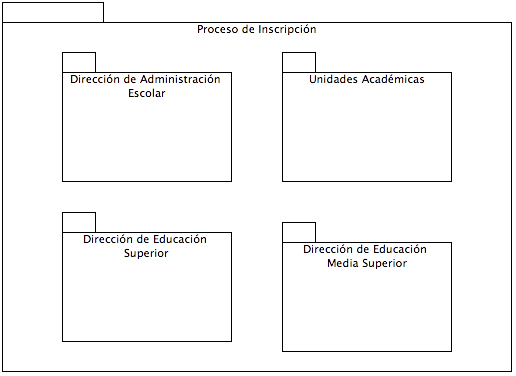
\includegraphics[width=0.7\textwidth]{dinamico/images/ArquitecturaLogica.png}}
		\caption{Diagrama de arquitectura lógica de inscripciones}
		\label{fig:arquitecturaIN}
	\end{center}
\end{figure}

%%		------------------------Diagrama de Dirección de Administración Escolar--------------------------
%		
%		La figura \ref{fig:PINDAE} muestra los submódulos para el módulo de la Dirección de Administración Escolar.\\
%		
%		\begin{figure}[htbp]
%			\begin{center}
%				\fbox{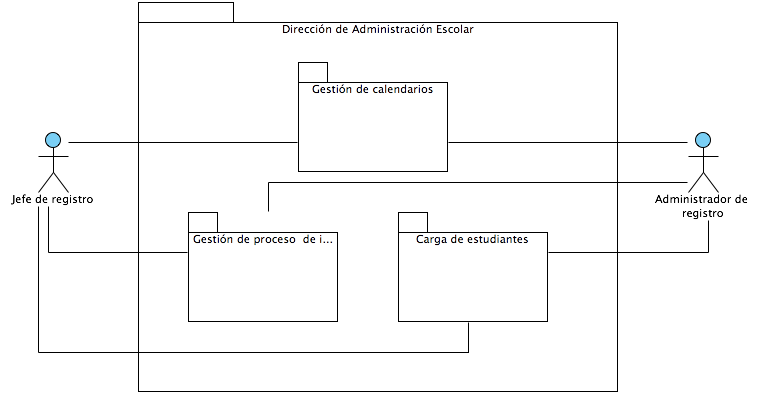
\includegraphics[width=0.9\textwidth]{dinamico/images/PIN_DAE.png}}
%				\caption{Módulo de la Dirección de Administración Escolar}
%				\label{fig:PINDAE}
%			\end{center}
%		\end{figure}
%	
%				La figura \ref{fig:PINDAEGestionDeCalendarios} muestra los casos de uso para el submódulo de Gestión de Calendarios, en el cual el \refElem{DAEAdministradorDeRegistro} podrá registrar la calendarización para las Unidades Académicas del Instituto.\\
%				
%				\begin{figure}[htbp]
%					\begin{center}
%						\fbox{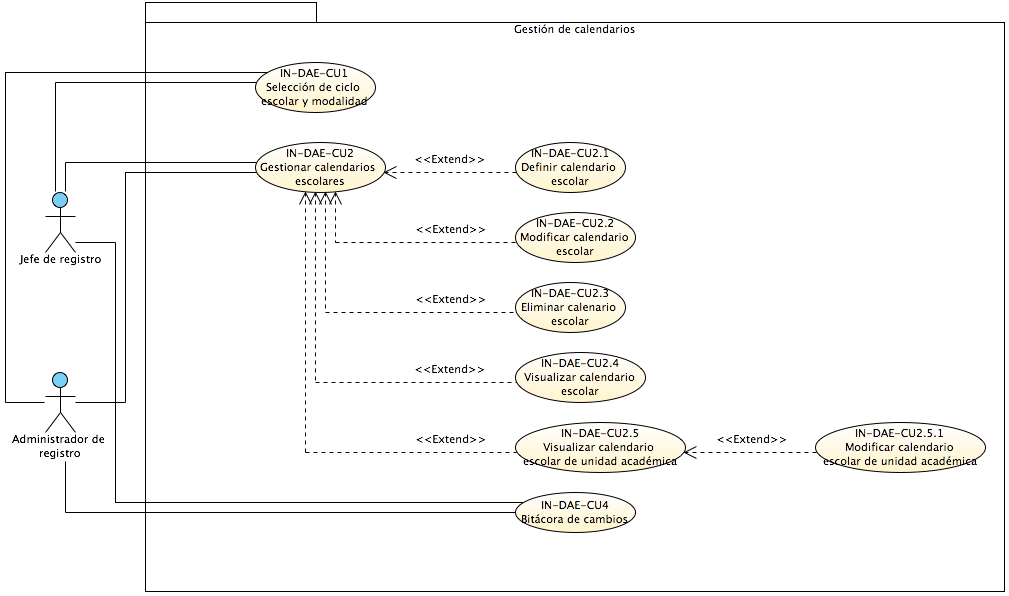
\includegraphics[width=0.9\textwidth]{dinamico/images/PIN_DAE_GestionDeCalendarios.png}}
%						\caption{Submódulo de Gestión de Calendarios}
%						\label{fig:PINDAEGestionDeCalendarios}
%					\end{center}
%				\end{figure}
%
%				La figura \ref{fig:PINDAEGestionDeProcesoDeInscripcion} muestra los casos de uso para el submódulo de Gestión de Proceso de Inscripción, en el cual el \refElem{DAEAdministradorDeRegistro} podrá administrar los procesos de inscripción registrados en el sistema, los cuales realizan la importación de estudiantes al Calmécac. \\
%
%				\begin{figure}[htbp]
%					\begin{center}
%						\fbox{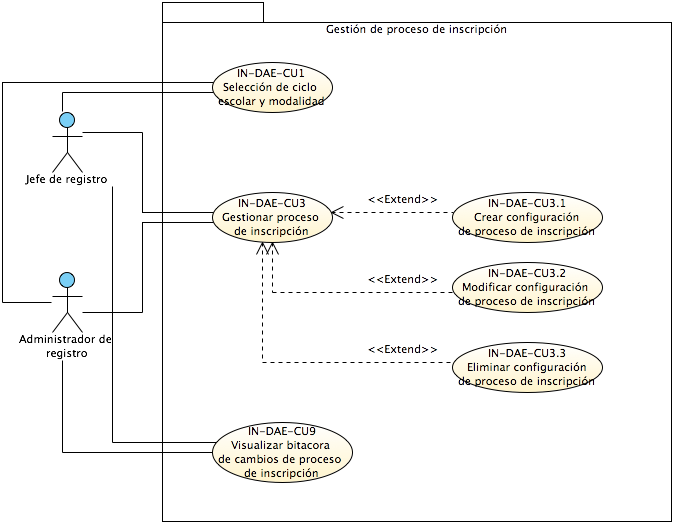
\includegraphics[width=0.9\textwidth]{dinamico/images/PIN_DAE_GestionDeProcesoDeInscripcion.png}}
%						\caption{Submódulo de Gestión de Proceso de Inscripción}
%						\label{fig:PINDAEGestionDeProcesoDeInscripcion}
%					\end{center}
%				\end{figure}
%			
%				La figura \ref{fig:PINDAECargaDeEstudiantes} muestra los casos de uso para el submódulo de Carga de Estudiantes, en el cual el \refElem{DAEAdministradorDeRegistro} podrá visualizar a los estudiantes de nuevo ingreso en el Instituto, estos pueden ser visualizados por Unidad Académica y Programa Académico.\\
%
%				\begin{figure}[htbp]
%					\begin{center}
%						\fbox{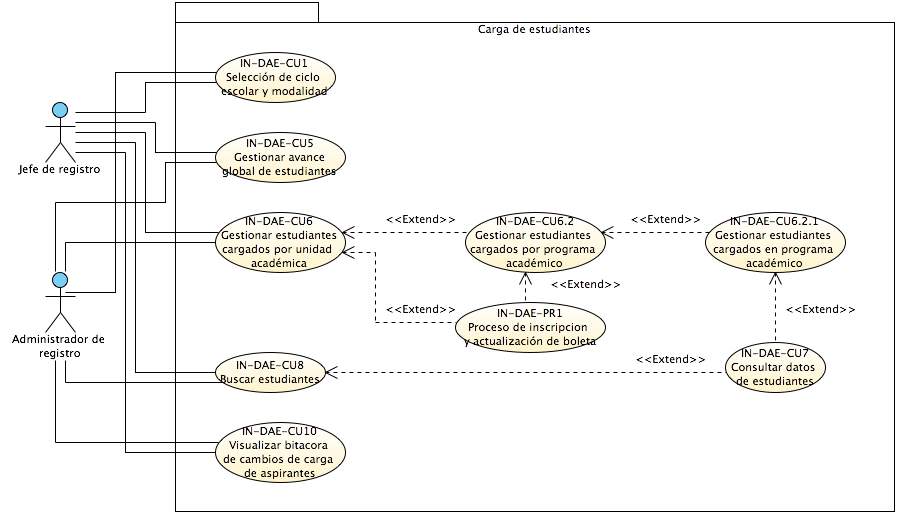
\includegraphics[width=0.9\textwidth]{dinamico/images/PIN_DAE_CargaDeEstudiantes.png}}
%						\caption{Submódulo de Carga de Estudiantes}
%						\label{fig:PINDAECargaDeEstudiantes}
%					\end{center}
%				\end{figure}
%			
%%		------------------------Diagrama de Dirección de Educación Superior--------------------------
%		
%		La figura \ref{fig:PINDES} muestra los submódulos para el módulo de la Dirección de Educación Superior.\\
%			
%		\begin{figure}[htbp]
%			\begin{center}
%				\fbox{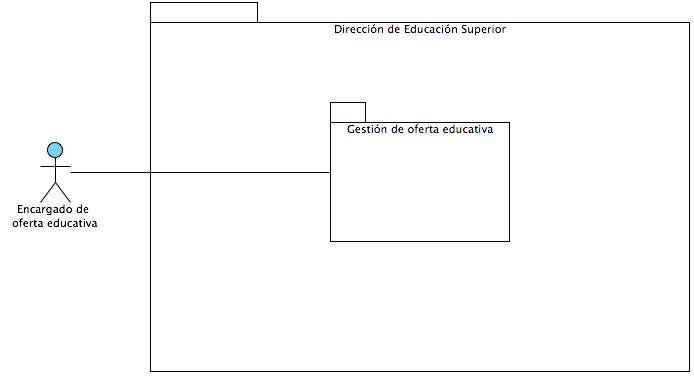
\includegraphics[width=0.9\textwidth]{dinamico/images/PIN_DES.png}}
%				\caption{Módulo de la Dirección de Educación Superior}
%				\label{fig:PINDES}
%			\end{center}
%		\end{figure}
%	
%				La figura \ref{fig:PINDESGestionDeOfertaEducativa} muestra los casos de uso para el submódulo de Gestión de Oferta Educativa, en el cual el \refElem{DESEncargadoDeOfertaEducativa} podrá registrar la oferta educativa para los Programas Académicos de las Unidades Académicas de nivel Superior.\\
%				
%				\begin{figure}[htbp]
%					\begin{center}
%						\fbox{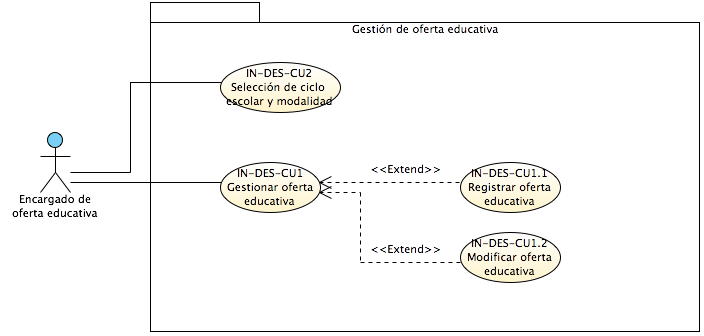
\includegraphics[width=0.9\textwidth]{dinamico/images/PIN_DES_GestionDeOfertaEducativa.png}}
%						\caption{Submódulo de Gestión de Oferta Educativa}
%						\label{fig:PINDESGestionDeOfertaEducativa}
%					\end{center}
%				\end{figure}
%				
%%		------------------------Diagrama de Dirección de Educación Media Superior--------------------------
%
%		La figura \ref{fig:PINDEMS} muestra los submódulos para el módulo de la Dirección de Educación Media Superior.\\
%		
%		\begin{figure}[htbp]
%			\begin{center}
%				\fbox{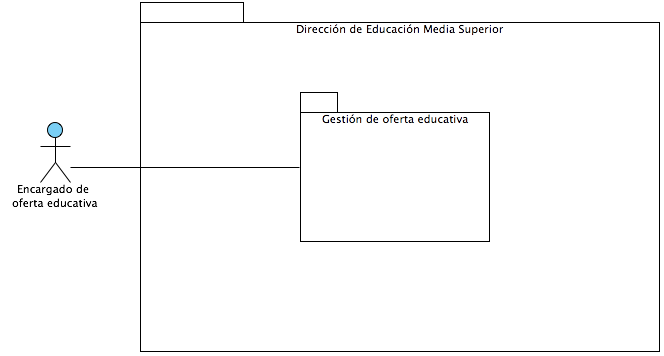
\includegraphics[width=0.9\textwidth]{dinamico/images/PIN_DEMS.png}}
%				\caption{Módulo de la Dirección de Educación Media Superior}
%				\label{fig:PINDEMS}
%			\end{center}
%		\end{figure}
%		
%				La figura \ref{fig:PINDEMSGestionDeOfertaEducativa} muestra los casos de uso para el submódulo de Gestión de Oferta Educativa, en el cual el \refElem{DESEncargadoDeOfertaEducativa} podrá registrar la oferta educativa para los Programas Académicos de las Unidades Académicas de nivel Superior.\\
%				
%				\begin{figure}[htbp]
%					\begin{center}
%						\fbox{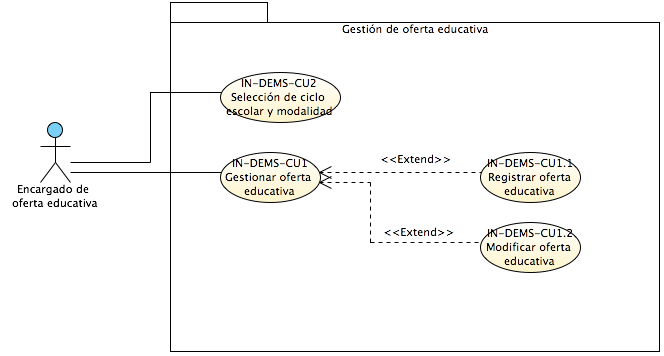
\includegraphics[width=0.9\textwidth]{dinamico/images/PIN_DEMS_GestionDeOfertaEducativa.png}}
%						\caption{Submódulo de Gestión de Oferta Educativa}
%						\label{fig:PINDEMSGestionDeOfertaEducativa}
%					\end{center}
%				\end{figure}
				
%		------------------------Diagrama de Unidad Académica --------------------------

		La figura \ref{fig:PINUA} muestra los submódulos para el módulo de Unidad Académica.\\
		
		\begin{figure}[htbp]
			\begin{center}
				\fbox{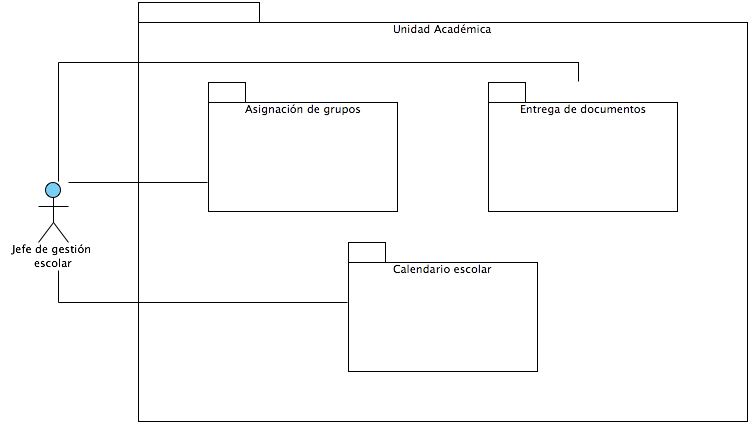
\includegraphics[width=0.9\textwidth]{dinamico/images/PIN_UA.png}}
				\caption{Módulo de Unidad Académica}
				\label{fig:PINUA}
			\end{center}
		\end{figure}
		
%				La figura \ref{fig:PINUAGestionDeCalendarios} muestra los casos de uso para el submódulo de Gestión de Calendarios, en el cual el \refElem{UAJefeDeGestionEscolar} podrá registrar la calendarización para su Unidad Académica.\\
%
%				\begin{figure}[htbp]
%					\begin{center}
%						\fbox{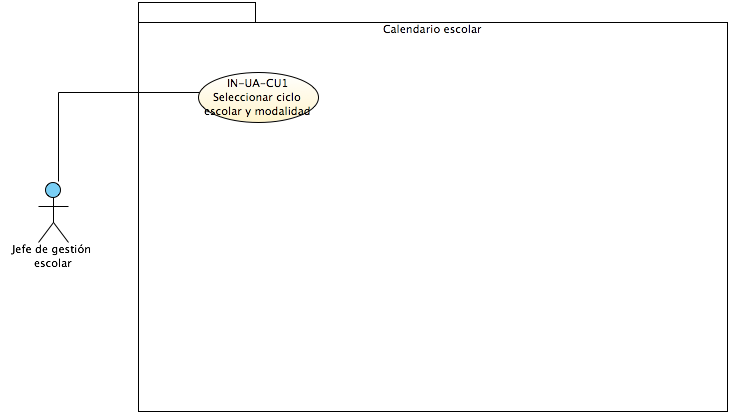
\includegraphics[width=0.9\textwidth]{dinamico/images/PIN_UA_CalendarioEscolar.png}}
%						\caption{Submódulo de Gestión de Calendarios}
%						\label{fig:PINUAGestionDeCalendarios}
%					\end{center}
%				\end{figure}
								
				La figura \ref{fig:PINUAAsignacionDeGrupos} muestra los casos de uso para el submódulo de Asignación de Grupos, en el cual el \refElem{UAJefeDeGestionEscolar} podrá asignarle grupos y Unidades de Aprendizaje a los estudiantes de nuevo ingreso de su Unidad Académica.\\

				\begin{figure}[htbp]
					\begin{center}
						\fbox{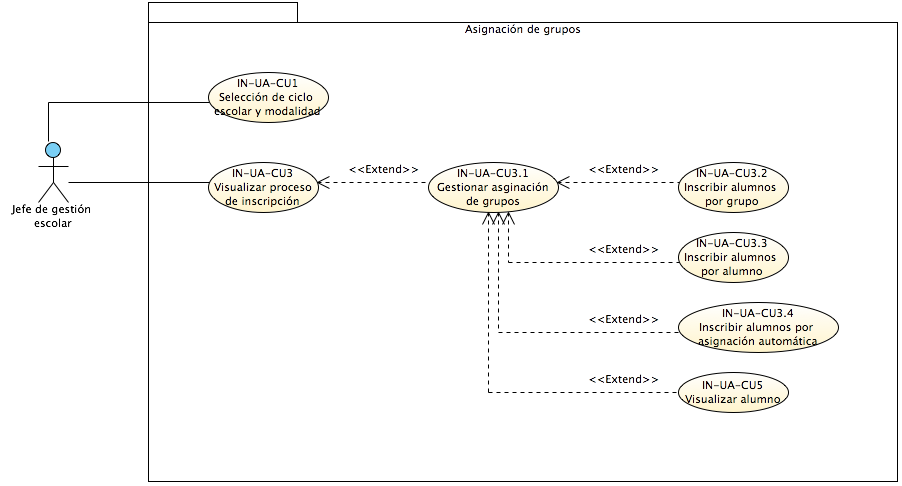
\includegraphics[width=0.9\textwidth]{dinamico/images/PIN_UA_AsignacionDeGrupos.png}}
						\caption{Submódulo de Asignación de Grupos}
						\label{fig:PINUAAsignacionDeGrupos}
					\end{center}
				\end{figure}

%				La figura \ref{fig:PINUAEntregaDeDocumentos} muestra los casos de uso para el submódulo de Entrega de Documentos, en el cual el \refElem{UAJefeDeGestionEscolar} podrá registrar la entrega de documentos de los estudiantes de nuevo ingreso.\\
%
%				\begin{figure}[htbp]
%					\begin{center}
%						\fbox{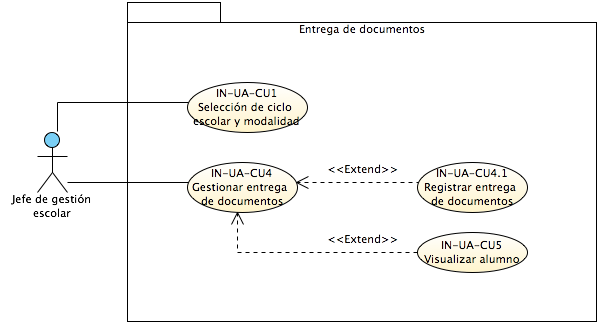
\includegraphics[width=0.9\textwidth]{dinamico/images/PIN_UA_EntregaDeDocumentos.png}}
%						\caption{Submódulo de Entrega de Documentos}
%						\label{fig:PINUAEntregaDeDocumentos}
%					\end{center}
%				\end{figure}

        
        %---------- Modelo de estados ----------
        \chapter{Modelo de estados}
        \label{ch:estados}
        %%%%% Modelo de estados de Entidades del sistema.
El presente capítulo describe el modelo de estados correspondiente a las entidades del Calmécac que tienen un comportamiento dinámico en el sistema. Está conformado por los siguientes elementos:
%\begin{itemize}
%	\item Modelo del ciclo de vida de la \refElem{EstructuraEducativa} de una \refElem{UnidadAcademica} en la sección \refElem{sec:SM-EE}, el cual describe la evolución de la Estructura Educativa desde que es creada hasta que es cerrada cuando termina el periodo para el que fue definida.
%	
%	\item Modelo del ciclo de vida de un elemento de la \refElem{EstructuraEducativa} en la sección \refElem{sec:SM-ElementoEE}, el cual describe la evolución de un elemento de la Estructura Educativa desde que es creado hasta que es aprobada o se le realizan cambios una vez que ha sido aprobada.
%\end{itemize}
%
%%% Máquina de estados general de la Estructura Educativa
%\begin{Maquina}{sec:SM-EE}{Modelo del ciclo de vida de la Estructura Educativa de una Unidad Académica}{
%En cualquier momento dado, la \refElem{tEstructuraEducativa} de una \refElem{tUnidadAcademica} correspondiente a un \refElem{tPeriodoEscolar} tiene un 'estado' en el sistema. Las acciones que los actores pueden realizar sobre la Estructura Educativa dependen de dicho estado y pueden tener como consecuencia la transición a otro. Un resumen de las acciones posibles sobre la Estructura Educativa dependiendo del estado se muestran en la Tabla \ref{SM:estadosEE}. 
%
%Los actores involucrados en el ciclo de vida de la Estructura Educativa son:
%\begin{itemize} 
%	\item \refElem{UAParticipanteEE}: Este actor engloba a todos los participantes de la definición de la Estructura Educativa dentro de la Unidad Académica. Cuando existen funciones que son particulares a un actor específico, se indican de forma separada para dicho actor como es el caso del \refElem{UAResponsableEstructuraEducativa}.
%	\item \refElem{DESAnalista}
%	\item \refElem{DESResponsableEE}
%\end{itemize}
% 
%
%Los estados y transiciones posibles del ciclo de vida de la Estructura Educativa se muestran en la Figura \ref{fig:sec:SM-EE} y se describen a continuación.	
%}{images/maquinasEstados/EstructuraEducativa.png}
%%\begin{figure}[htbp!]
%%	\centering
%%	\fbox{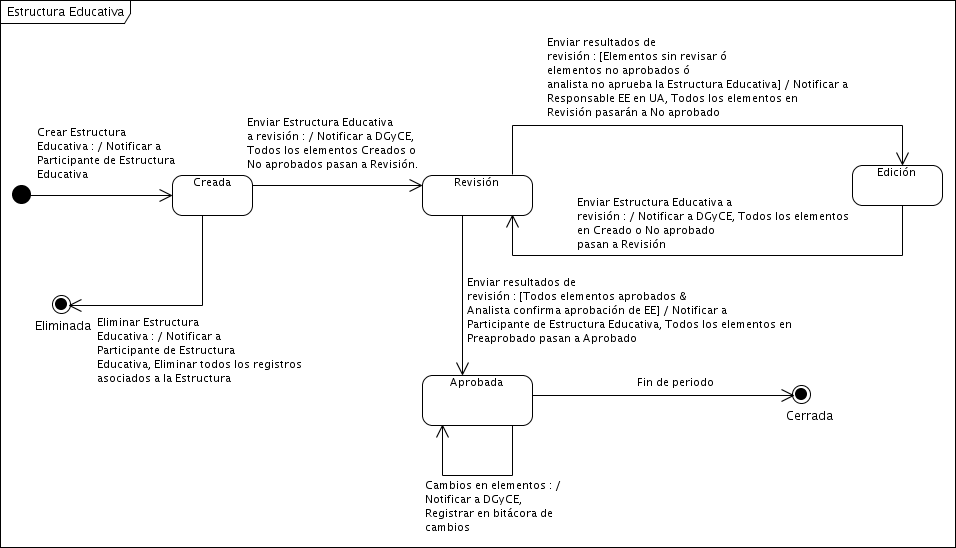
\includegraphics[width=\textwidth]{images/maquinasEstados/EstructuraEducativa.png}}
%%	\caption{Modelo del ciclo de vida de la Estructura Educativa}
%%	\label{fig:maquinaEstadosEE}
%%\end{figure}
%
%\begin{description}
%
%% ESTADO: Creada
%\item[Creada:] Este es el estado con el que inicia la Estructura Educativa después de que ha sido creada, ya sea en blanco o como copia de la Estructura Educativa de algún periodo anterior. Cuando la Estructura Educativa es creada, se notifica de su creación a los participantes de la misma ( ver \refElem{UAParticipanteEE} ). Estar en este estado significa que los componentes de la Estructura están siendo gestionados por parte del \refElem{UAParticipanteEE} y que la Estructura Educativa acaba de ser creada y no ha sido enviada para Revisión de la DGyCE. Para la Estructura estar en este estado implica que:
%
%\begin{description}
%	\item[\refElem{UAParticipanteEE}:] Este actor puede:
%	\begin{itemize} 
%		\item Modificar los elementos que la conforman de acuerdo con el estado del elemento.
%		\item Modificar los horarios asociados con elementos creados.
%		\item Consultar los elementos que la conforman.
%		\item Añadir elementos.
%		\item Eliminar elementos que la conforman.
%	\end{itemize}
%	
%	
%	\item[\refElem{UAResponsableEstructuraEducativa}:] Este actor puede:
%	\begin{itemize} 
%%		\item Cambiar su configuración.
%		
%		\item Enviarla para revisión, resultando en la transición hacia el estado {\bf Revisión}, la transición hacia el estado {\bf Revisión} de todos los elementos que no han sido aprobados y el envío de una notificación al \refElem{DESAnalista} y \refElem{DESResponsableEE} indicando que existen elementos de la Estructura Educativa listos para revisión.
%		
%		\item Eliminarla, resultando en la transición hacia el estado {\bf Eliminada} y el envío de una notificación a cada \refIdElem{UAParticipanteEE} indicándole que la Estructura Educativa ha sido eliminada.
%	\end{itemize}	
%	
%	\item[\refElem{DESAnalista}:] Este actor no tiene acceso a la Estructura Educativa.
%	
%	\item[\refElem{DESResponsableEE}:] Este actor no tiene acceso a la Estructura Educativa.
%	
%\end{description}
%
%% ESTADO: Revisión
%\item[Revisión:] En este estado la Estructura Educativa está siendo revisada por \refElem{DESAnalista} o \refElem{DESResponsableEE} quienes pueden determinar si aprueban o no cada elemento de forma independiente. En este estado no se permite la modificación de horarios asociados a los elementos en revisión. Para la Estructura Educativa, estar en este estado implica que:%Al terminar la revisión de todos los elementos que se encuentran en estado {\bf Revisión}, se da pie a dos posibles transiciones:
%%\begin{itemize} 
%%	\item Hacia el estado {\bf Edición} si existe al menos un elemento cuyo estado no es {\bf Aprobado} o, ya sea el \refElem{DESAnalista} o el \refElem{DESResponsableEE}, no confirma la aprobación de la Estructura. Esto causa que todos los elementos que se encontraban en {\bf Revisión} cambien de estado a {\bf Edición} y se le notifique al \refElem{UAResponsableEstructuraEducativa} que la Estructura Educativa no ha sido aprobada.
%%	
%%	\item Hacia el estado {\bf Aprobada} si todos los elementos existentes han sido aprobados y el \refElem{DESAnalista} o \refElem{DESResponsableEE} confirman la aprobación de la Estructura. Cuando esto ocurre, se le notifica al \refElem{UAResponsableEstructuraEducativa} la aprobación de la Estructura Educativa.
%%\end{itemize}
%
%
%\begin{description}
%	\item[\refElem{UAParticipanteEE}:] Este actor puede:% consultar los elementos que la conforman.
%	\begin{itemize} 
%		\item Modificar los elementos que la conforman de acuerdo con el estado del elemento.
%		\item Consultar los elementos que la conforman.
%		\item Añadir elementos.
%		\item Modificar los horarios asociados con elementos creados.
%		\item Eliminar elementos de acuerdo con el estado del elemento.
%	\end{itemize}
%	
%	\item[\refElem{DESAnalista}:] Este actor puede:
%	\begin{itemize} 
%		\item Consultar los elementos que la conforman.
%		\item Revisar los elementos, lo que puede tener dos posibles resultados: aprobarlos o no.
%		\item Realizar observaciones sobre los elementos.
%		\item Enviar a la Unidad Académica los resultados de la revisión, lo que da pie a dos posibles transiciones:
%		\begin{itemize} 
%			\item Hacia el estado {\bf Edición} si existen elementos sin revisar (en estado {\bf Revisión}), elementos cuyo estado es {\bf No Aprobado} o, ya sea el \refElem{DESAnalista} o el \refElem{DESResponsableEE}, no aprueban la Estructura. Esto causa que todos los elementos que se encontraban en {\bf Revisión} cambien de estado a {\bf No aprobado} y se le notifique al \refElem{UAResponsableEstructuraEducativa} que la Estructura Educativa no ha sido aprobada.
%			
%			\item Hacia el estado {\bf Aprobada} si todos los elementos existentes han sido aprobados y el \refElem{DESAnalista} o \refElem{DESResponsableEE} aprueba la Estructura. Cuando esto ocurre, se le notifica al \refElem{UAResponsableEstructuraEducativa} la aprobación de la Estructura Educativa.
%		\end{itemize}
%	\end{itemize}
%	
%	\item[\refElem{DESResponsableEE}:] Este actor puede:
%	\begin{itemize} 
%		\item Consultar los elementos que la conforman.
%		\item Revisar los elementos, lo que puede tener dos posibles resultados: aprobarlos o no.
%		\item Realizar observaciones sobre los elementos.
%		\item Enviar a la Unidad Académica los resultados de la revisión, lo que da pie a dos posibles transiciones:
%		\begin{itemize} 
%			\item Hacia el estado {\bf Edición} si existen elementos sin revisar (en estado {\bf Revisión}), elementos cuyo estado es {\bf No Aprobado} o, ya sea el \refElem{DESAnalista} o el \refElem{DESResponsableEE}, no aprueban la Estructura. Esto causa que todos los elementos que se encontraban en {\bf Revisión} cambien de estado a {\bf No aprobado} y se le notifique al \refElem{UAResponsableEstructuraEducativa} que la Estructura Educativa no ha sido aprobada.
%			
%			\item Hacia el estado {\bf Aprobada} si todos los elementos existentes han sido aprobados y el \refElem{DESAnalista} o \refElem{DESResponsableEE} aprueba la Estructura. Cuando esto ocurre, se le notifica al \refElem{UAResponsableEstructuraEducativa} la aprobación de la Estructura Educativa.
%		\end{itemize}
%	\end{itemize}
%\end{description}
%
%
%
%% ESTADO: Edición
%\item[Edición:] Este es el estado en el que se encuentra la Estructura Educativa después de que ha sido revisada y no fue aprobada, ya sea debido a que existen elementos creados o no aprobados (ver \refElem{sec:SM-ElementoEE} ) o el \refElem{DESAnalista} no la ha aprobado. Estar en este estado significa que los componentes de la Estructura están siendo gestionados por parte del \refElem{UAParticipanteEE}. Para la Estructura estar en estado implica que:
%
%\begin{description}
%	\item[\refElem{UAParticipanteEE}:] Este actor puede:
%		\begin{itemize} 
%			\item Modificar los elementos que la conforman de acuerdo con el estado del elemento.
%			\item Consultar los elementos que la conforman.
%			\item Modificar los horarios asociados con los elementos.
%			\item Añadir elementos.
%			\item Eliminar elementos de acuerdo con el estado del elemento.
%		\end{itemize}
%
%	\item[\refElem{UAResponsableEstructuraEducativa}:] Este actor puede enviarla para revisión, resultando en la transición hacia el estado {\bf Revisión}, la transición hacia el estado {\bf Revisión} de todos los elementos que no han sido aprobados y el envío de una notificación al \refElem{DESAnalista} y \refElem{DESResponsableEE} indicando que existen elementos de la Estructura Educativa listos para revisión. 
%		
%	
%	\item[\refElem{DESAnalista}:] Este actor puede consultar los elementos que han sido aprobados previamente.
%			
%	\item[\refElem{DESResponsableEE}:] Este actor puede consultar los elementos que han sido aprobados previamente.
%	
%\end{description}
%
%% ESTADO: Aprobada
%\item[Aprobada:] En este estado la Estructura Educativa ha sido aprobada por la DGyCE. Se pueden realizar cambios en la Estructura los cuales quedarán registrados en la bitácora de cambios y producen una transición a este mismo estado. Es posible agregar o eliminar elementos y estas acciones también quedarán registrados en la bitácora de cambios. Es partir de este estado que la Estructura Educativa puede ser copiada para servir de base a Estructuras Educativas futuras. Para la estructura estar en este estado implica que:
%	\begin{description}
%		\item[\refElem{UAParticipanteEE}:] Este actor puede:
%		\begin{itemize} 
%			\item Modificar los elementos que la conforman de acuerdo con el estado del elemento.
%			\item Consultar los elementos que la conforman.
%			\item Añadir elementos.
%			\item Modificar los horarios asociados con los elementos.
%			\item Eliminar elementos de acuerdo con el estado del elemento.
%		\end{itemize}
%		
%		\item[\refElem{DESAnalista}:] Este actor puede consultar los elementos que ya han sido aprobados.
%		
%		\item[\refElem{DESResponsableEE}:] Este actor puede consultar los elementos que ya han sido aproabdos.
%	\end{description}
%
%% ESTADO: Cerrada
%\item[Cerrada:] Este es el estado al que pasa la Estructura Educativa una vez que el periodo para el que fue definida concluye. En este estado todos los actores involucrados pueden consultar sus elementos pero no se admite ningún tipo de modificación. 
%
%% ESTADO: Eliminada
%\item[Eliminada:] Este estado indica que la Estructura Educativa ha sido eliminada del sistema y por lo tanto ningún actor puede realizar operación alguna sobre ella. Cuando esto ocurre, todos los elementos de la Estructura también se eliminan.
%
%\end{description}
%
%
%\begin{longtable}{| p{0.35\textwidth} | p{0.6\textwidth} |}
%	\hline  
%	\label{SM:estadosEE} 
%	{\bf Estado de Estructura Educativa}  & {\bf Acciones sobre Estructura Educativa}\\
%	\endfirsthead
%	\hline
%	Creada & 
%	\begin{Titemize} 
%		\Titem Agregar elementos.
%		\Titem Modificar los horarios asociados con elementos.
%		\Titem Editar elementos
%		\Titem Eliminar elementos
%		\Titem Consultar elementos
%		\Titem Enviarla a revisión
%		\Titem Eliminarla
%%		\Titem Realizar observaciones sobre los elementos
%%		\Titem Revisar elementos
%%		\Titem Enviar resultados de revisión
%	\end{Titemize}\\ 
%	\hline
%	Revisión &  
%	\begin{Titemize} 
%		\Titem Agregar elementos.
%		\Titem Modificar los horarios asociados con elementos que no se encuentren en revisión.
%		\Titem Editar elementos que no se encuentren en revisión.
%		\Titem Eliminar elementos que no se encuentren en revisión.
%		\Titem Consultar elementos
%		\Titem Realizar observaciones sobre los elementos
%		\Titem Revisar elementos
%		\Titem Enviar resultados de revisión
%	\end{Titemize}\\ 
%	\hline
%	No Aprobada & 
%	\begin{Titemize} 
%		\Titem Agregar elementos.
%		\Titem Modificar los horarios asociados con elementos.
%		\Titem Editar elementos
%		\Titem Eliminar elementos
%		\Titem Consultar elementos
%		\Titem Enviarla a revisión
%	\end{Titemize}\\
%	\hline
%	Aprobada & 
%	\begin{Titemize} 
%		\Titem Agregar elementos.
%		\Titem Modificar los horarios asociados con elementos.
%		\Titem Editar elementos
%		\Titem Eliminar elementos
%		\Titem Consultar elementos
%		\Titem Realizar una copia para una Estructura Educativa futura.
%	\end{Titemize}\\ 
%	\hline
%	Cerrada  & 
%	\begin{Titemize} 
%		\Titem Consultar elementos
%		\Titem Realizar una copia para una Estructura Educativa futura.
%	\end{Titemize}\\ 
%	\hline
%	Eliminada & Ninguna\\ 
%	\hline
%	\caption{Acciones que se pueden realizar sobre una Estructura Educativa dependiendo de su estado}
%\end{longtable}
%\end{Maquina}
%
%%% Máquina de estados de un elemento de la Estructura Educativa
%\begin{Maquina}{sec:SM-ElementoEE}{Modelo del ciclo de vida de un Elemento de la Estructura Educativa de una Unidad Académica} {
%En cualquier momento dado, un elemento de la \refElem{tEstructuraEducativa} de una \refElem{tUnidadAcademica} correspondiente a un \refElem{tPeriodo} y a una \refElem{tModalidad} tiene un 'estado' en el sistema. 
%
%Se entiende por elemento de la Estructura Educativa al registro de un docente en alguno de los formatos de Soporte Documental.
%
%Las acciones que los actores pueden realizar sobre un elemento dependen de su estado y del estado de la Estructura Educativa a la que pertenece ( ver \refElem{sec:SM-EE} ) y pueden tener como consecuencia la transición a otro. Las posibles combinaciones de estados entre ambas máquinas y las acciones posibles sobre los elementos se muestran en la Tabla \ref{SM:combinatoriaEstados}.
%
%Los actores involucrados en el ciclo de vida de un Elemento de la Estructura Educativa son:
%\begin{itemize} 
%	\item \refElem{UAParticipanteEE}: Este actor engloba a todos los que participan en la definición de la Estructura Educativa dentro de la Unidad Académica. Cuando existen funciones que son particulares a un actor específico, se indican de forma separada para dicho actor.
%	\item \refElem{DESAnalista}
%	\item \refElem{DESResponsableEE}
%\end{itemize}
%
%Los estados y transiciones posibles del ciclo de vida de un Elemento de la Estructura Educativa se muestran en la figura \ref{fig:sec:SM-ElementoEE} y se describen a continuación.	
%%
%%\begin{figure}[htbp!]
%%	\centering
%%	\fbox{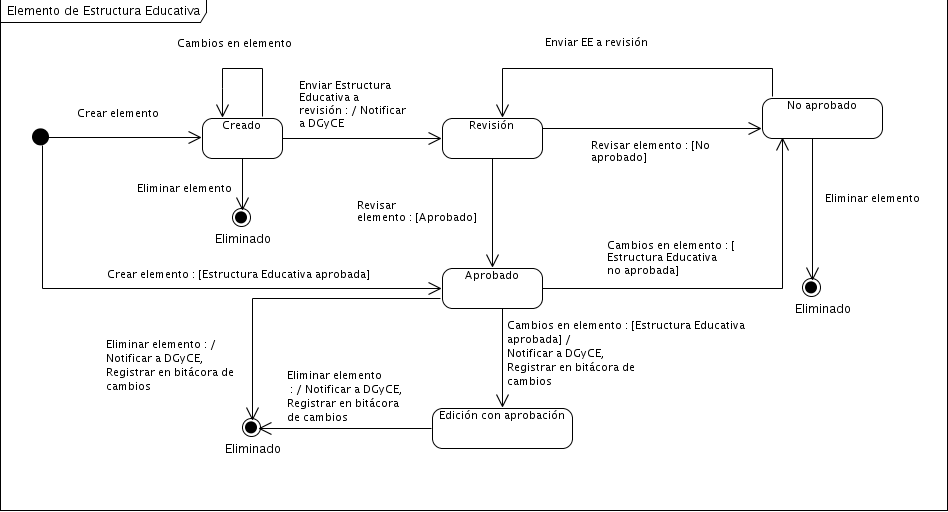
\includegraphics[width=\textwidth]{images/maquinasEstados/ElementoEstructuraEducativa.png}}
%%	\caption{Modelo del ciclo de vida de un Elemento de la Estructura Educativa}
%%	\label{fig:maquinaEstadosElementoEE}
%%\end{figure}
%}{images/maquinasEstados/ElementoEstructuraEducativa.png}
%\begin{description}
%
%% ESTADO: Edición
%\item[Creado:] Este es el estado en el que comienza el elemento de la Estructura Educativa una vez que ha sido creado y la Estructura Educativa a la que pertenece no ha sido aprobada. El elemento pudo haber sido fue agregado o copiado de una Estructura Educativa de un periodo anterior. Estar en este estado significa que el elemento está siendo editado por el \refElem{UAParticipanteEE}. Existen dos posibles transiciones que salen de este estado:
%\begin{itemize} 
%	\item Hacia el estado {\bf Revisión} cuando la Estructura Educativa a la que pertenece es enviada a revisión
%	\item Hacia este estado cuando se realizan cambios en el elemento.
%\end{itemize}
%
%Para el elemento, estar en este estado implica que:
%	\begin{description}
%		\item[\refElem{UAParticipanteEE}:] Este actor puede:
%		\begin{itemize} 
%			\item Editarlo
%			\item Eliminarlo, resultando en una transición hacia el estado {\bf Eliminado}.
%			\item Consultarlo
%			\item Enviarlo a revisión
%			\item Modificar los horarios a los que está asociado.
%			%\item Revisarlo
%			%\item Hacerle observaciones
%		\end{itemize}
%	
%		\item[\refElem{DESAnalista}:] Este actor no tiene acceso al elemento.
%		
%		\item[\refElem{DESResponsableEE}:] Este actor no tiene acceso al elemento.
%	\end{description}
%
%% ESTADO: Revisión
%\item[Revisión:] El elemento pasa a este estado cuando la Estructura Educativa es enviada a revisión (ver \refElem{sec:SM-EE}) y significa que está siendo revisado por \refElem{DESAnalista} o \refElem{DESResponsableEE}. Para el elemento, estar en estado implica que:
%	\begin{description}
%		\item[\refElem{UAParticipanteEE}:] Este actor puede consultarlo.
%		
%		\item[\refElem{DESAnalista}:] Este actor puede:
%		\begin{itemize} 
%			\item Consultarlo.
%			\item Hacerle observaciones
%			\item Revisarlo, dando pie a dos transiciones posibles:
%			\begin{itemize} 
%				\item Hacia el estado {\bf Edición} en caso de que no apruebe el elemento, lo que produce el envío de una notificación al \refElem{UAResponsableEstructuraEducativa} indicándole que el elemento no ha sido aprobado.
%				\item Hacia el estado {\bf Aprobado} en caso de que apruebe el elemento.
%			\end{itemize}
%		\end{itemize}
%	
%		\item[\refElem{DESResponsableEE}:] Este actor puede:
%		\begin{itemize} 
%			\item Consultarlo.
%			\item Hacerle observaciones
%			\item Revisarlo, dando pie a dos transiciones posibles:
%			\begin{itemize} 
%				\item Hacia el estado {\bf Edición} en caso de que no apruebe el elemento, lo que produce el envío de una notificación al \refElem{UAResponsableEstructuraEducativa} indicándole que el elemento no ha sido aprobado.
%				\item Hacia el estado {\bf Aprobado} en caso de que apruebe el elemento.
%			\end{itemize}
%		\end{itemize}
%	
%	\end{description}
%
%% ESTADO: Preaprobado
%%\item[Preaprobado:] En este estado el elemento de la Estructura Educativa ha sido aprobado pero la Estructura Educativa a la que pertenece no. En este estado se pueden realizar cambios en el elemento sin que estos se reflejen en la bitácora o eliminarlo en caso de que sea necesario. Cuando la Estructura Educativa a la que pertenece el elemento es aprobada, todos los elementos que se encuentren en este estado pasan a {\bf Aprobado}. Para el elemento, estar en este estado implica que:
%%\begin{description}
%%	\item[\refElem{UAParticipanteEE}:] Este actor puede:
%%	\begin{itemize} 
%%		\item Consultarlo
%%		\item Eliminarlo, siempre y cuando la Estructura Educativa a la que pertenece esté en {\bf Edición}, resultando en una transición hacia el estado {\bf Eliminado}
%%		\item Modificarlo, siempre y cuando la Estructura Educativa a la que pertenece esté en {\bf Edición}, resultando en una transición hacia el estado {\bf Edición}.
%%	\end{itemize}
%%	
%%	\item[\refElem{DESAnalista}:] Este actor puede consultarlo.
%%	
%%	\item[\refElem{DESResponsableEE}:] Este actor puede consultarlo.	
%%	
%%\end{description}
%
%
%% ESTADO: Aprobado
%\item[Aprobado:] El elemento pasa a este estado cuando el resultado de su revisón es aprobado o cuando la Estructura Educativa está aprobada al momento de su creación. Si lo último ocurre, la creación se registra en la bitácora de cambios y se le notifica al \refElem{DESAnalista} de la creación. Se pueden realizar cambios al elemento en este estado considerando que todo cambio que se haga se registra en la bitácora de cambios. Para el elemento, estar en este estado implica que:
%	\begin{description}
%		\item[\refElem{UAParticipanteEE}:] Este actor puede:
%		\begin{itemize} 
%			\item Editarlo, dando pie a dos posibles transiciones:
%			\begin{itemize} 
%				\item Hacia el estado {\bf No aprobado} si la Estructura Educativa no se encuentra aprobada.
%				\item Hacia el estado {\bf Edición con aprobación} si la Estructura Educativa se encuentra aprobada, lo que resulta en el registro de la moficación en la bitácora de cambios y en envío de una notificación al \refElem{DESAnalista} para comunicarle que hubo un cambio en el elemento.
%			\end{itemize} 
%			\item Eliminarlo, resultando en una transición hacia el estado {\bf Eliminado}, el registro de la eliminación en la bitácora de cambios y el envío de una notificación al \refElem{DESAnalista} para comunicarle la eliminación.
%			\item Consultarlo 
%			\item Modificar los horarios a los que está asociado.
%		\end{itemize}
%	
%		\item[\refElem{DESAnalista}:] Este actor puede consultarlo.
%
%		\item[\refElem{DESResponsableEE}:] Este actor puede consultarlo.	
%	
%	\end{description}
%	
%% ESTADO: Edición con aprobación	
%\item[Edición con aprobación:] Estar en este estado significa que el elemento ha sido modificado después de haber sido aprobado. Para el elemento, estar en este estado implica que:
%	\begin{description}
%		\item[\refElem{UAParticipanteEE}:] Este actor puede:
%		\begin{itemize} 
%			\item Editarlo, resultando en el envío de una notificación al \refElem{DESAnalista} indicándole del cambio.
%			\item Eliminarlo, resultando en una transición hacia el estado {\bf Eliminado}, el registro de la eliminación en la bitácora de cambios y el envío de una notificación al \refElem{DESAnalista} indicándole de la eliminación
%			\item Consultarlo 
%			\item Modificar los horarios a los que está asociado.
%		\end{itemize}
%		
%		\item[\refElem{DESAnalista}:] Este actor puede consultarlo.
%		
%		\item[\refElem{DESResponsableEE}:] Este actor puede consultarlo.
%
%	\end{description}
%
%%ESTADO: Eliminado
%\item[Eliminado:] Este estado indica que el Elemento de la Estructura Educativa ha sido eliminado del sistema y por lo tanto ningún actor puede realizar operación alguna sobre él.
%
%\end{description}
%
%\begin{longtable}{| p{.12\textwidth} | p{.12\textwidth} | p{.06\textwidth}| p{.07\textwidth}| p{.1\textwidth}| p{.1\textwidth}| p{.1\textwidth}| p{.1\textwidth}| p{.1\textwidth}| }
%	\hline  
%	\rowcolor{colorPrincipal}
%	\multicolumn{9}{|c|}{\bf\color{white}{Tabla de Estados}}\\\hline
%	\label{SM:combinatoriaEstados} 
%	{\bf Estado de Estructura Educativa} & {\bf Estado de Elemento de Estructura Educativa} & {\bf Editar} & {\bf Eliminar} & {\bf Consultar} & {\bf Enviar a revisión}  & {\bf Modificar horarios asociados} & {\bf Revisar} & {\bf Hacer observaciones}\\
%	\endfirsthead
%%	\hline\multicolumn{1}{|c|}{\textbf{Estado de Estructura Educativa}} &
%%	\multicolumn{1}{|c|}{\textbf{Estado de Elemento de Estructura Educativa}} &
%%	\multicolumn{1}{c|}{\textbf{Acciones sobre elemento}} \\ \hline 
%%	\endhead
%	\hline
%	Creada & Creado & Sí & Sí & Sí & Sí  & Sí & No & No\\
%	\hline
%	Creada & Revisión & \multicolumn{7}{c|}{No válido}\\
%	\hline
%	Creada & No aprobado & \multicolumn{7}{c|}{No válido}\\
%	\hline
%	Creada & Aprobado & \multicolumn{7}{c|}{No válido}\\
%	\hline
%	Creada & Edición con aprobación & \multicolumn{7}{c|}{No válido}\\
%	\hline
%	Revisión & Creado & Sí & Sí & Sí & No & Sí & No & No\\
%	\hline
%	Revisión & Revisión & No & No & Sí & No & No & Sí & Sí\\
%	\hline
%	Revisión & No aprobado & No & No & Sí & No & No & No & No\\
%	\hline
%	Revisión & Aprobado & No & No & Sí & No & No & No & No\\
%	\hline
%	Revisión & Edición con aprobación & No & No & Sí & No & No & No & No\\
%	\hline
%	Edición & Creado & Sí & Sí & Sí & No & Sí & No & No\\
%	\hline
%	Edición & Revisión & \multicolumn{7}{c|}{No válido}\\
%	\hline
%	Edición & No aprobado & Sí & Sí & Sí & No & Sí & No & No\\
%	\hline
%	Edición & Aprobado & Sí & Sí & Sí & No & Sí & No & No\\
%	\hline
%	Edición & Edición con aprobación & Sí & Sí & Sí & No & Sí & No & No\\
%	\hline
%	Aprobada & Creado & \multicolumn{7}{c|}{No válido}\\
%	\hline
%	Aprobada & Revisión & \multicolumn{7}{c|}{No válido}\\
%	\hline
%	Aprobada & No aprobado & \multicolumn{7}{c|}{No válido}\\
%	\hline
%	Aprobada & Aprobado & Sí & Sí & Sí & No & Sí & No & No\\
%	\hline
%	Aprobada & Edición con aprobación & Sí & Sí & Sí & No & Sí & No & No\\
%	\hline
%	Cerrada & Cualquiera & No & No & Sí & No & No & No & No\\
%	\hline
%	\caption{Combinaciones posibles de estados del ciclo de vida de una Estructura Educativa y un Elemento de la Estructura Educativa y acciones posibles sobre el elemento.}
%\end{longtable}
%
%\end{Maquina}

        
        %---------- Modelo de actores ----------
        \chapter{Modelo de actores}
        \label{ch:actores}
        % !TEX root = ../integrado.tex
%=============================================
% Descripción de actores
\label{chapter:ActoresDelSistema}

	En el presente capítulo se definen los participantes en los procesos actuales y fortalecidos. Se da una breve descripción de cada uno, la mayoría tomada de la normatividad correspondiente: Reglamento General, Reglamento interno y Manuales de operación del IPN, entre otros. Aquellas descripciones tomadas de la normatividad tienen la referencia del documento de dónde fueron tomadas, en algunos casos los actores son propuestos para poder llevar a cabo algunas de las tareas en el \refElem{Calmecac}.

\section{Descripción de Actores}

Cada participante se describe con la siguiente estructura:

\begin{objetivos}[Descripción de participantes]
	\item {\bf Nombre:} Nombre con el que se le conoce al participante dentro del negocio.
	\item {\bf Descripción:} Descripción breve del perfil, puesto o rol que juega el participante.
	\item {\bf Área:} En caso de que el participante pertenezca a una estructura se indica el área, departamento o ubicación al que pertenece o se encuentra.
	\item {\bf Responsabilidades:} Se listan las responsabilidades oficiales o relacionadas con el Calmécac según aplique. En el caso de las descripciones tomadas de la normatividad se listan todas.
	\item {\bf Perfil:} Cuando se reconoce un nivel de conocimientos, preparación o capacidades determinadas para desarrollar una participación se describen, con la finalidad de ser tomado en cuenta para el desarrollo del sistema.
	\item {\bf Fuente:} Referencia al documento base de donde fue tomada dicha descripción.
\end{objetivos}

Cuando el participante es un departamento o dirección, se omite el dato ``Perfil'' es un Sistema de Información los datos que se describen son:

\begin{objetivos}[Descripción de sistemas]
	\item {\bf Nombre:} Nombre o siglas del sistema.
	\item {\bf Descripción:} Descripción breve del sistema.
	\item {\bf Área:} Área al que le pertenece, opera o es responsable del sistema.
	\item {\bf Responsabilidades:} Funciones principales del sistema.
	\item {\bf Lenguaje:} Tecnologías principales o plataforma utilizadas en su desarrollo.
	\item {\bf Fuente:} Referencia al documento base de donde fue tomada dicha descripción.
\end{objetivos}

\section{Participantes detectados}

La figura \ref{fig:actoresIN} muestra los actores que participan en el módulo de inscripciones. En particular los actores del submódulo de DAE, DES y UA. %El \refElem{UAResponsableEstructuraEducativa} hereda todas las características de los actores \refElem{UAResponsableHorarios} y \refElem{UAResponsableSD}. 

\begin{figure}[htbp]
	\begin{center}
		\fbox{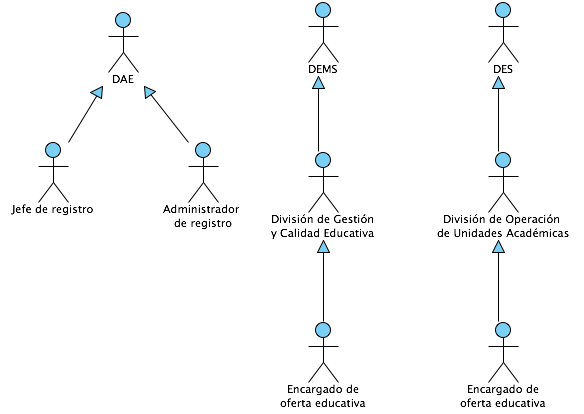
\includegraphics[width=0.7\textwidth]{dinamico/images/Actores_IN}}
		\caption{Actores del módulo de inscripciones}
		\label{fig:actoresIN}
	\end{center}
\end{figure}

%%========== DAEJefeDeRegistro ======%
%\begin{actor}{DAEJefeDeRegistro}{Jefe de Registro}{Persona encarga de registrar los calendarios escolares de las Unidades Académicas y definir el periodo de los procesos de inscripción en el Calmécac.}
%	\item[Área:] \refElem{tDAE}
%	\item[Responsabilidades:] \cdtEmpty
%	\begin{itemize}
%		\item Definir la oferta educativa para los diferentes programas académicos que hay en la unidad académica en sus distintas modalidades para el siguiente periodo escolar.
%		\item Definir la cantidad de grupos a utilizar para la oferta educativa de la unidad académica para el siguiente periodo escolar.
%		\item Asignar unidades de aprendizaje a los grupos que se utilizaran para le siguiente periodo escolar.
%		\item Definir los horarios de las unidades de aprendizaje asignadas a los grupos.
%		\item Definir más de un laboratorio a las unidades de aprendizaje que lo requieran.
%		\item Asignar profesores a las unidades de aprendizaje que se ofertarán para el próximo periodo escolar.
%		\item Asignar a todos los profesores basificados su carga máxima de horas frente a grupo.
%		\item Asignar a los profesores interinos las unidades de aprendizaje 
%		\item Definir un periodo para la recepción de las solicitudes de aprendizaje que son enviadas por los profesores.
%	\end{itemize}
%		\item[Fuente:]%Reglamento General de Estudios, Manual de Organización de la Secretaría Académica
%		%\item[Solicitado por:] 
%\end{actor}
%
%
%========== Responsable de Horarios en la UA ======%
%\begin{actor}{DAEAdministradorDeRegistro}{Administrador de Registro}{Persona encarga de registrar los calendarios escolares de las Unidades Académicas, definir el periodo de los procesos de inscripción en el Calmécac y asignar permisos a usuarios del área.}
%	\item[Área:] \refElem{tDAE}
%	\item[Responsabilidades:] \cdtEmpty
%	\begin{itemize}
%		\item Monitorear las solicitudes de unidades de aprendizaje de los profesores
%		\item Enviar una notificación a los profesores que no halla enviado aún su solicitud de unidades de aprendizaje antes de que se acabe el periodo para la recepción de solicitudes.
%		\item Consultar las solicitudes de los profesores para las diferentes academias que existen en la unidad académica.
%	\end{itemize}
%		\item[Fuente:]%Reglamento General de Estudios, Manual de Organización de la Secretaría Académica
%		%\item[Solicitado por:] 
%\end{actor}
%
%
%%========== DESAdministrador ======%
%\begin{actor}{DESEncargadoDeOfertaEducativa}{Encargado de Oferta Educativa}{Persona encargada de dar seguimiento al proceso de inscripción en la DES.}
%	\item[Área:] \refElem{tDES}
%	\item[Responsabilidades:] \cdtEmpty
%		\begin{itemize}
%			\item Proporcionar información sobre las carreras y lugares ofertados.
%			\item Dar seguimiento al proceso de inscripciones y cambios de carrera.
%		\end{itemize}
%	\item[Fuente:]
%\end{actor}
%
%%========== UAJefeDeControlEscolar ======%
\begin{actor}{UAJefeDeGestionEscolar}{Jefe de Gestión Escolar}{Persona encargada de operar el departamento de Control Escolar de una Unidad Académica.}
	\item[Área:] \refElem{tUA}
	\item[Responsabilidades:] \cdtEmpty
		\begin{itemize}
			\item Operar el CALMÉCAC dentro de la Unidad Académica.
			\item Operar y dirigir el proceso de Reinscripciones junto con el personal de Control Escolar de la Unidad Académica.
		\end{itemize}
	\item[Fuente:]
\end{actor}

        
        %----------pInscripciones---------------------

        \chapter{Casos de Uso del módulo de la Dirección de Administración Escolar}
        \label{ch:CUpInscripcionesDAE}
        % Sprint 3

%% !TEX root = ../../../integrado.tex

\begin{UseCase}{IN-DAE-CU4.2}{Modificar evaluación de E.T.S.}{
		Permite modificar el periodo de E.T.S. asignado a una unidad académica durante un ciclo escolar y modalidad determinada, redefiniendo la fecha de inicio y fin de:
		\begin{itemize}
			\item Periodo de E.T.S.
			\item Registro de E.T.S.
			\item Aplicación de E.T.S.
			\item Registro de evaluación.
		\end{itemize}
	}
	\UCccitem{Versión}{0.1}
	\UCccsection{Datos para el control Interno}	
	\UCccitem{Elaboró}{Alan Fernando Rincón Vieyra}
	\UCccitem{Supervisó}{Eduardo Espino Maldonado}
	\UCccitem{Operación}{Modificar}
	\UCccitem{Prioridad}{Alta}
	\UCccitem{Complejidad}{Media}
	\UCccitem{Volatilidad}{Media}
	\UCccitem{Madurez}{Baja}
	\UCccitem{Estatus}{Por revisar}
	\UCccitem{Dificultades}{
		\begin{Titemize}
			\Titem Regla de negocio de periodo válido.
			\Titem Modelo de información de los periodos de E.T.S.
			\Titem Especificar cómo se usará el tipo de E.T.S.
			\Titem ¿Quienes son los actores?
		\end{Titemize}
	}
	\UCccitem{Fecha del último estatus}{09 de Enero del 2018}
	\UCccsection{Revisión Versión 0.1}
	\UCccitem{Fecha}{}
	\UCccitem{Evaluador}{}
	\UCccitem{Resultado}{}
	\UCccitem{Observaciones}{}
	\UCsection{Atributos}
	\UCitem{Actores}{
		\begin{Titemize}
			\Titem \refElem{Actor}
		\end{Titemize}
	}
	\UCitem{Propósito}{Mantener actualizadas las fechas de los periodos de registro, aplicación y evaluación de E.T.S. que cada \refElem{tUnidadAcademica} realiza durante un \refElem{tCicloEscolar} y \refElem{tModalidad} determinada.}
	
	\UCitem{Entradas}{
		\begin{Titemize}
			\Titem \refElem{ActividadCalendario.fechaInicio} y \refElem{ActividadCalendario.fechaFin} del periodo de E.T.S.
			\Titem \refElem{ActividadCalendario.fechaInicio} y \refElem{ActividadCalendario.fechaFin} del \refElem{Actividad.registroDeETS}.
			\Titem \refElem{ActividadCalendario.fechaInicio} y \refElem{ActividadCalendario.fechaFin} de la \refElem{Actividad.aplicacionDeETS}.
			\Titem \refElem{ActividadCalendario.fechaInicio} y \refElem{ActividadCalendario.fechaFin} del \refElem{Actividad.registroDeEvaluacion}.
		\end{Titemize}
	}
	\UCitem{Origen}{
		\begin{Titemize}
			\Titem Se selecciona con el mouse.
		\end{Titemize}
	}
	\UCitem{Salidas}{
		\begin{Titemize}
			\Titem \refElem{ActividadCalendario.fechaInicio} y \refElem{ActividadCalendario.fechaFin} actualizadas para las actividades del Periodo de E.T.S. modificado.
		\end{Titemize}
	}
	\UCitem{Destino}{Pantalla}
	\UCitem{Precondiciones}{
		\begin{Titemize}
			\Titem \textbf{Sistematizada:} Que se haya seleccionado previamente un \refElem{CicloEscolar}, una \refElem{tModalidad} y una \refElem{tUnidadAcademica}.
			\Titem \textbf{Sistematizada:} Que exista al menos un Periodo de E.T.S. registrado en el sistema.
		\end{Titemize}
	}
	\UCitem{Postcondiciones}{
		\begin{Titemize}
			\Titem Se actualiza en el sistema la información del Periodo de E.T.S., el cual permite a los alumnos inscribirse a los mismos.
		\end{Titemize}
	}
	\UCitem{Reglas de Negocio}{
		\begin{Titemize}
			\Titem \refIdElem{BR-IN-S015}
			\Titem \refIdElem{BR-IN-S016}
			\Titem \refIdElem{BR-IN-S017}
		\end{Titemize}
	}
	\UCitem{Errores}{
		\begin{Titemize}
			\Titem \UCerr{Uno}{Cuando se ha establecido un Periodo de E.T.S. inválido}{se muestra el mensaje \refIdElem{MSG18} y regresa al paso \ref{IN-DAE-CU4.2:seleccionarPeriodo} de la trayectoria principal.}
			\Titem \UCerr{Dos}{Cuando se ha establecido un periodo de Registro de E.T.S. inválido}{se muestra el mensaje \refIdElem{MSG18} y regresa al paso \ref{IN-DAE-CU4.2:seleccionarRegistro} de la trayectoria principal.}
			\Titem \UCerr{Tres}{Cuando se ha establecido un periodo de Registro de E.T.S. fuera del
				Periodo de E.T.S.}{se muestra el mensaje \refIdElem{MSG130} y regresa al paso \ref{IN-DAE-CU4.2:seleccionarRegistro} de la trayectoria principal.}
			\Titem \UCerr{Cuatro}{Cuando se ha establecido un periodo de Aplicación de E.T.S. inválido}{se muestra el mensaje \refIdElem{MSG18} y regresa al paso \ref{IN-DAE-CU4.2:seleccionarAplicacion} de la trayectoria principal.}
			\Titem \UCerr{Cinco}{Cuando se ha establecido un periodo de Aplicación de E.T.S. fuera del
				Periodo de E.T.S.}{se muestra el mensaje \refIdElem{MSG130} y regresa al paso \ref{IN-DAE-CU4.2:seleccionarAplicacion} de la trayectoria principal.}
			\Titem \UCerr{Seis}{Cuando se ha establecido un periodo de Aplicación de E.T.S. antes o durante el periodo de Registro de E.T.S.}{se muestra el mensaje \refIdElem{MSG130} y regresa al paso \ref{IN-DAE-CU4.2:seleccionarAplicacion} de la trayectoria principal.}
			\Titem \UCerr{Siete}{Cuando se ha establecido un periodo de Registro de evaluación inválido}{se muestra el mensaje \refIdElem{MSG18} y regresa al paso \ref{IN-DAE-CU4.2:seleccionarEvaluacion} de la trayectoria principal.}
			\Titem \UCerr{Ocho}{Cuando se ha establecido un periodo de Registro de evaluación fuera del
				Periodo de E.T.S.}{se muestra el mensaje \refIdElem{MSG130} y regresa al paso \ref{IN-DAE-CU4.2:seleccionarEvaluacion} de la trayectoria principal.}
			\Titem \UCerr{Nueve}{Cuando se ha establecido un periodo de Registro de evaluación antes de la fecha de inicio del periodo de Aplicación de E.T.S.}{se muestra el mensaje \refIdElem{MSG130} y regresa al paso \ref{IN-DAE-CU4.2:seleccionarEvaluacion} de la trayectoria principal.}
		\end{Titemize}
	}
	
	\UCitem{Viene de}{\refIdElem{IN-DAE-CU4}}
	\UCitem{Disparador}{
		\begin{Titemize}
			\Titem El actor requiere Modificar un periodo de E.T.S.
		\end{Titemize}
	}
	
	\UCitem{Condiciones de Término}{
		\begin{Titemize}
			\Titem Se muestra la información actualizada del Periodo de E.T.S. seleccionado.
		\end{Titemize}
	}
	\UCitem{Efectos Colaterales}{Ninguno}
	\UCitem{Referencia Documental}{C1-PF Proceso Fortalecido}
	\UCitem{Auditable}{Si, se registra el usuario, la fecha y la acción que realizó.}
	\UCitem{Datos sensibles}{Ninguno}
\end{UseCase}


%Trayectoria Principal : Happy Path


\begin{UCtrayectoria}
	\UCpaso[\UCactor]  \label{IN-DAE-CU4.2:seleccionarPeriodo} Solicita modificar un Periodo de E.T.S. dando clic en el ícono {\IUCalendario} del campo \refElem{ActividadCalendario.fechaInicio} o \refElem{ActividadCalendario.fechaFin} en la pantalla \refIdElem{IN-DAE-IU4}. \refTray{A} \refTray{B} \refTray{C} \refTray{D}
	
	\UCpaso Verifica si el Periodo de E.T.S. seleccionado es válido con base en la regla de negocio \refIdElem{BR-N0X1}. \refErr{Uno}
	
	\UCpaso Modifica el Periodo de E.T.S.
	
	\UCpaso Muestra el mensaje \refIdElem{MSG1} indicando que la modificación del Periodo de E.T.S. se realizo de manera exitosa.
\end{UCtrayectoria}

%Trayectorias Alternativas

\begin{UCtrayectoriaA}[Fin del caso de uso.]{A}{El actor desea modificar un periodo de Registro de E.T.S.}
	\UCpaso[\UCactor]  \label{IN-DAE-CU4.2:seleccionarRegistro} Solicita modificar un periodo de Registro de E.T.S. dando clic en el ícono {\IUCalendario} del campo \refElem{ActividadCalendario.fechaInicio} o \refElem{ActividadCalendario.fechaFin} en la pantalla \refIdElem{IN-DAE-IU4}.
	\UCpaso Verifica si el periodo de Registro de E.T.S. seleccionado es válido con base en la regla de negocio \refIdElem{BR-N0X1}. \refErr{Dos}
	\UCpaso Verifica si el periodo de Registro de E.T.S. seleccionado se encuentra dentro del
	Periodo de E.T.S. definido previamente en el \refIdElem{IN-DAE-CU4.1} con base en la regla de negocio \refIdElem{BR-IN-S015}. \refErr{Tres}
	\UCpaso Modifica el periodo de Registro de E.T.S.
	\UCpaso Muestra el mensaje \refIdElem{MSG1} indicando que la modificación del periodo de Registro de E.T.S. se realizo de manera exitosa.
\end{UCtrayectoriaA}

\begin{UCtrayectoriaA}[Fin del caso de uso.]{B}{El actor desea modificar un periodo de Aplicación de E.T.S.}
	\UCpaso[\UCactor]  \label{IN-DAE-CU4.2:seleccionarAplicacion} Solicita modificar un periodo de Aplicación de E.T.S. dando clic en el ícono {\IUCalendario} del campo \refElem{ActividadCalendario.fechaInicio} o \refElem{ActividadCalendario.fechaFin} en la pantalla \refIdElem{IN-DAE-IU4}.
	\UCpaso Verifica si el periodo de Aplicación de E.T.S. seleccionado es válido con base en la regla de negocio \refIdElem{BR-N0X1}. \refErr{Cuatro}
	\UCpaso Verifica si el periodo de Aplicación de E.T.S. seleccionado se encuentra dentro del
	Periodo de E.T.S. definido en el \refIdElem{IN-DAE-CU4.1} con base en la regla de negocio \refIdElem{BR-IN-S015}. \refErr{Cinco}
	\UCpaso Verifica que el periodo de Aplicación de E.T.S. seleccionado sea posterior al periodo de Registro de E.T.S. definido en el \refIdElem{IN-DAE-CU4.1} con base en la regla de negocio \refIdElem{BR-IN-S016}. \refErr{Seis}
	\UCpaso Modifica el periodo de Aplicación de E.T.S.
	\UCpaso Muestra el mensaje \refIdElem{MSG1} indicando que la modificación del periodo de Aplicación de E.T.S. se realizo de manera exitosa.
\end{UCtrayectoriaA}

\begin{UCtrayectoriaA}[Fin del caso de uso.]{C}{El actor desea modificar un periodo de Registro de evaluación.}
	\UCpaso[\UCactor]  \label{IN-DAE-CU4.2:seleccionarEvaluacion} Solicita modificar un periodo de Registro de evaluación. dando clic en el ícono {\IUCalendario} del campo \refElem{ActividadCalendario.fechaInicio} o \refElem{ActividadCalendario.fechaFin} en la pantalla \refIdElem{IN-DAE-IU4}.
	\UCpaso Verifica si el periodo de Registro de evaluación seleccionado es válido con base en la regla de negocio \refIdElem{BR-N0X1}. \refErr{Siete}
	\UCpaso Verifica si el periodo de Registro de evaluación seleccionado se encuentra dentro del
	Periodo de E.T.S. definido en el \refIdElem{IN-DAE-CU4.1} con base en la regla de negocio \refIdElem{BR-IN-S015}. \refErr{Ocho}
	\UCpaso Verifica que el periodo de Registro de evaluación seleccionado sea posterior o igual a la fecha de inicio del periodo de Aplicación de E.T.S. definido en el \refIdElem{IN-DAE-CU4.1} con base en la regla de negocio \refIdElem{BR-IN-S017}. \refErr{Nueve}
	\UCpaso Modifica el periodo de Registro de evaluación.
	\UCpaso Muestra el mensaje \refIdElem{MSG1} indicando que la modificación del periodo de Registro de evaluación se realizo de manera exitosa.
\end{UCtrayectoriaA}

\begin{UCtrayectoriaA}[Fin del caso de uso.]{D}{El actor desea cancelar la operación.}
	\UCpaso[\UCactor] Solicita cancelar la operación presionando el botón \IUbutton{Regresar}.
	\UCpaso Muestra la pantalla \refIdElem{IN-DAE-UI2.5}.
\end{UCtrayectoriaA}
%% !TEX root = ../../../integrado.tex

\begin{UseCase}{IN-DAE-CU4.2}{Modificar evaluación de E.T.S.}{
		Permite modificar el periodo de E.T.S. asignado a una unidad académica durante un ciclo escolar y modalidad determinada, redefiniendo la fecha de inicio y fin de:
		\begin{itemize}
			\item Periodo de E.T.S.
			\item Registro de E.T.S.
			\item Aplicación de E.T.S.
			\item Registro de evaluación.
		\end{itemize}
	}
	\UCccitem{Versión}{0.1}
	\UCccsection{Datos para el control Interno}	
	\UCccitem{Elaboró}{Alan Fernando Rincón Vieyra}
	\UCccitem{Supervisó}{Eduardo Espino Maldonado}
	\UCccitem{Operación}{Modificar}
	\UCccitem{Prioridad}{Alta}
	\UCccitem{Complejidad}{Media}
	\UCccitem{Volatilidad}{Media}
	\UCccitem{Madurez}{Baja}
	\UCccitem{Estatus}{Por revisar}
	\UCccitem{Dificultades}{
		\begin{Titemize}
			\Titem Regla de negocio de periodo válido.
			\Titem Modelo de información de los periodos de E.T.S.
			\Titem Especificar cómo se usará el tipo de E.T.S.
			\Titem ¿Quienes son los actores?
		\end{Titemize}
	}
	\UCccitem{Fecha del último estatus}{09 de Enero del 2018}
	\UCccsection{Revisión Versión 0.1}
	\UCccitem{Fecha}{}
	\UCccitem{Evaluador}{}
	\UCccitem{Resultado}{}
	\UCccitem{Observaciones}{}
	\UCsection{Atributos}
	\UCitem{Actores}{
		\begin{Titemize}
			\Titem \refElem{Actor}
		\end{Titemize}
	}
	\UCitem{Propósito}{Mantener actualizadas las fechas de los periodos de registro, aplicación y evaluación de E.T.S. que cada \refElem{tUnidadAcademica} realiza durante un \refElem{tCicloEscolar} y \refElem{tModalidad} determinada.}
	
	\UCitem{Entradas}{
		\begin{Titemize}
			\Titem \refElem{ActividadCalendario.fechaInicio} y \refElem{ActividadCalendario.fechaFin} del periodo de E.T.S.
			\Titem \refElem{ActividadCalendario.fechaInicio} y \refElem{ActividadCalendario.fechaFin} del \refElem{Actividad.registroDeETS}.
			\Titem \refElem{ActividadCalendario.fechaInicio} y \refElem{ActividadCalendario.fechaFin} de la \refElem{Actividad.aplicacionDeETS}.
			\Titem \refElem{ActividadCalendario.fechaInicio} y \refElem{ActividadCalendario.fechaFin} del \refElem{Actividad.registroDeEvaluacion}.
		\end{Titemize}
	}
	\UCitem{Origen}{
		\begin{Titemize}
			\Titem Se selecciona con el mouse.
		\end{Titemize}
	}
	\UCitem{Salidas}{
		\begin{Titemize}
			\Titem \refElem{ActividadCalendario.fechaInicio} y \refElem{ActividadCalendario.fechaFin} actualizadas para las actividades del Periodo de E.T.S. modificado.
		\end{Titemize}
	}
	\UCitem{Destino}{Pantalla}
	\UCitem{Precondiciones}{
		\begin{Titemize}
			\Titem \textbf{Sistematizada:} Que se haya seleccionado previamente un \refElem{CicloEscolar}, una \refElem{tModalidad} y una \refElem{tUnidadAcademica}.
			\Titem \textbf{Sistematizada:} Que exista al menos un Periodo de E.T.S. registrado en el sistema.
		\end{Titemize}
	}
	\UCitem{Postcondiciones}{
		\begin{Titemize}
			\Titem Se actualiza en el sistema la información del Periodo de E.T.S., el cual permite a los alumnos inscribirse a los mismos.
		\end{Titemize}
	}
	\UCitem{Reglas de Negocio}{
		\begin{Titemize}
			\Titem \refIdElem{BR-IN-S015}
			\Titem \refIdElem{BR-IN-S016}
			\Titem \refIdElem{BR-IN-S017}
		\end{Titemize}
	}
	\UCitem{Errores}{
		\begin{Titemize}
			\Titem \UCerr{Uno}{Cuando se ha establecido un Periodo de E.T.S. inválido}{se muestra el mensaje \refIdElem{MSG18} y regresa al paso \ref{IN-DAE-CU4.2:seleccionarPeriodo} de la trayectoria principal.}
			\Titem \UCerr{Dos}{Cuando se ha establecido un periodo de Registro de E.T.S. inválido}{se muestra el mensaje \refIdElem{MSG18} y regresa al paso \ref{IN-DAE-CU4.2:seleccionarRegistro} de la trayectoria principal.}
			\Titem \UCerr{Tres}{Cuando se ha establecido un periodo de Registro de E.T.S. fuera del
				Periodo de E.T.S.}{se muestra el mensaje \refIdElem{MSG130} y regresa al paso \ref{IN-DAE-CU4.2:seleccionarRegistro} de la trayectoria principal.}
			\Titem \UCerr{Cuatro}{Cuando se ha establecido un periodo de Aplicación de E.T.S. inválido}{se muestra el mensaje \refIdElem{MSG18} y regresa al paso \ref{IN-DAE-CU4.2:seleccionarAplicacion} de la trayectoria principal.}
			\Titem \UCerr{Cinco}{Cuando se ha establecido un periodo de Aplicación de E.T.S. fuera del
				Periodo de E.T.S.}{se muestra el mensaje \refIdElem{MSG130} y regresa al paso \ref{IN-DAE-CU4.2:seleccionarAplicacion} de la trayectoria principal.}
			\Titem \UCerr{Seis}{Cuando se ha establecido un periodo de Aplicación de E.T.S. antes o durante el periodo de Registro de E.T.S.}{se muestra el mensaje \refIdElem{MSG130} y regresa al paso \ref{IN-DAE-CU4.2:seleccionarAplicacion} de la trayectoria principal.}
			\Titem \UCerr{Siete}{Cuando se ha establecido un periodo de Registro de evaluación inválido}{se muestra el mensaje \refIdElem{MSG18} y regresa al paso \ref{IN-DAE-CU4.2:seleccionarEvaluacion} de la trayectoria principal.}
			\Titem \UCerr{Ocho}{Cuando se ha establecido un periodo de Registro de evaluación fuera del
				Periodo de E.T.S.}{se muestra el mensaje \refIdElem{MSG130} y regresa al paso \ref{IN-DAE-CU4.2:seleccionarEvaluacion} de la trayectoria principal.}
			\Titem \UCerr{Nueve}{Cuando se ha establecido un periodo de Registro de evaluación antes de la fecha de inicio del periodo de Aplicación de E.T.S.}{se muestra el mensaje \refIdElem{MSG130} y regresa al paso \ref{IN-DAE-CU4.2:seleccionarEvaluacion} de la trayectoria principal.}
		\end{Titemize}
	}
	
	\UCitem{Viene de}{\refIdElem{IN-DAE-CU4}}
	\UCitem{Disparador}{
		\begin{Titemize}
			\Titem El actor requiere Modificar un periodo de E.T.S.
		\end{Titemize}
	}
	
	\UCitem{Condiciones de Término}{
		\begin{Titemize}
			\Titem Se muestra la información actualizada del Periodo de E.T.S. seleccionado.
		\end{Titemize}
	}
	\UCitem{Efectos Colaterales}{Ninguno}
	\UCitem{Referencia Documental}{C1-PF Proceso Fortalecido}
	\UCitem{Auditable}{Si, se registra el usuario, la fecha y la acción que realizó.}
	\UCitem{Datos sensibles}{Ninguno}
\end{UseCase}


%Trayectoria Principal : Happy Path


\begin{UCtrayectoria}
	\UCpaso[\UCactor]  \label{IN-DAE-CU4.2:seleccionarPeriodo} Solicita modificar un Periodo de E.T.S. dando clic en el ícono {\IUCalendario} del campo \refElem{ActividadCalendario.fechaInicio} o \refElem{ActividadCalendario.fechaFin} en la pantalla \refIdElem{IN-DAE-IU4}. \refTray{A} \refTray{B} \refTray{C} \refTray{D}
	
	\UCpaso Verifica si el Periodo de E.T.S. seleccionado es válido con base en la regla de negocio \refIdElem{BR-N0X1}. \refErr{Uno}
	
	\UCpaso Modifica el Periodo de E.T.S.
	
	\UCpaso Muestra el mensaje \refIdElem{MSG1} indicando que la modificación del Periodo de E.T.S. se realizo de manera exitosa.
\end{UCtrayectoria}

%Trayectorias Alternativas

\begin{UCtrayectoriaA}[Fin del caso de uso.]{A}{El actor desea modificar un periodo de Registro de E.T.S.}
	\UCpaso[\UCactor]  \label{IN-DAE-CU4.2:seleccionarRegistro} Solicita modificar un periodo de Registro de E.T.S. dando clic en el ícono {\IUCalendario} del campo \refElem{ActividadCalendario.fechaInicio} o \refElem{ActividadCalendario.fechaFin} en la pantalla \refIdElem{IN-DAE-IU4}.
	\UCpaso Verifica si el periodo de Registro de E.T.S. seleccionado es válido con base en la regla de negocio \refIdElem{BR-N0X1}. \refErr{Dos}
	\UCpaso Verifica si el periodo de Registro de E.T.S. seleccionado se encuentra dentro del
	Periodo de E.T.S. definido previamente en el \refIdElem{IN-DAE-CU4.1} con base en la regla de negocio \refIdElem{BR-IN-S015}. \refErr{Tres}
	\UCpaso Modifica el periodo de Registro de E.T.S.
	\UCpaso Muestra el mensaje \refIdElem{MSG1} indicando que la modificación del periodo de Registro de E.T.S. se realizo de manera exitosa.
\end{UCtrayectoriaA}

\begin{UCtrayectoriaA}[Fin del caso de uso.]{B}{El actor desea modificar un periodo de Aplicación de E.T.S.}
	\UCpaso[\UCactor]  \label{IN-DAE-CU4.2:seleccionarAplicacion} Solicita modificar un periodo de Aplicación de E.T.S. dando clic en el ícono {\IUCalendario} del campo \refElem{ActividadCalendario.fechaInicio} o \refElem{ActividadCalendario.fechaFin} en la pantalla \refIdElem{IN-DAE-IU4}.
	\UCpaso Verifica si el periodo de Aplicación de E.T.S. seleccionado es válido con base en la regla de negocio \refIdElem{BR-N0X1}. \refErr{Cuatro}
	\UCpaso Verifica si el periodo de Aplicación de E.T.S. seleccionado se encuentra dentro del
	Periodo de E.T.S. definido en el \refIdElem{IN-DAE-CU4.1} con base en la regla de negocio \refIdElem{BR-IN-S015}. \refErr{Cinco}
	\UCpaso Verifica que el periodo de Aplicación de E.T.S. seleccionado sea posterior al periodo de Registro de E.T.S. definido en el \refIdElem{IN-DAE-CU4.1} con base en la regla de negocio \refIdElem{BR-IN-S016}. \refErr{Seis}
	\UCpaso Modifica el periodo de Aplicación de E.T.S.
	\UCpaso Muestra el mensaje \refIdElem{MSG1} indicando que la modificación del periodo de Aplicación de E.T.S. se realizo de manera exitosa.
\end{UCtrayectoriaA}

\begin{UCtrayectoriaA}[Fin del caso de uso.]{C}{El actor desea modificar un periodo de Registro de evaluación.}
	\UCpaso[\UCactor]  \label{IN-DAE-CU4.2:seleccionarEvaluacion} Solicita modificar un periodo de Registro de evaluación. dando clic en el ícono {\IUCalendario} del campo \refElem{ActividadCalendario.fechaInicio} o \refElem{ActividadCalendario.fechaFin} en la pantalla \refIdElem{IN-DAE-IU4}.
	\UCpaso Verifica si el periodo de Registro de evaluación seleccionado es válido con base en la regla de negocio \refIdElem{BR-N0X1}. \refErr{Siete}
	\UCpaso Verifica si el periodo de Registro de evaluación seleccionado se encuentra dentro del
	Periodo de E.T.S. definido en el \refIdElem{IN-DAE-CU4.1} con base en la regla de negocio \refIdElem{BR-IN-S015}. \refErr{Ocho}
	\UCpaso Verifica que el periodo de Registro de evaluación seleccionado sea posterior o igual a la fecha de inicio del periodo de Aplicación de E.T.S. definido en el \refIdElem{IN-DAE-CU4.1} con base en la regla de negocio \refIdElem{BR-IN-S017}. \refErr{Nueve}
	\UCpaso Modifica el periodo de Registro de evaluación.
	\UCpaso Muestra el mensaje \refIdElem{MSG1} indicando que la modificación del periodo de Registro de evaluación se realizo de manera exitosa.
\end{UCtrayectoriaA}

\begin{UCtrayectoriaA}[Fin del caso de uso.]{D}{El actor desea cancelar la operación.}
	\UCpaso[\UCactor] Solicita cancelar la operación presionando el botón \IUbutton{Regresar}.
	\UCpaso Muestra la pantalla \refIdElem{IN-DAE-UI2.5}.
\end{UCtrayectoriaA}
%% !TEX root = ../../../integrado.tex

\begin{UseCase}{IN-DAE-CU4.2}{Modificar evaluación de E.T.S.}{
		Permite modificar el periodo de E.T.S. asignado a una unidad académica durante un ciclo escolar y modalidad determinada, redefiniendo la fecha de inicio y fin de:
		\begin{itemize}
			\item Periodo de E.T.S.
			\item Registro de E.T.S.
			\item Aplicación de E.T.S.
			\item Registro de evaluación.
		\end{itemize}
	}
	\UCccitem{Versión}{0.1}
	\UCccsection{Datos para el control Interno}	
	\UCccitem{Elaboró}{Alan Fernando Rincón Vieyra}
	\UCccitem{Supervisó}{Eduardo Espino Maldonado}
	\UCccitem{Operación}{Modificar}
	\UCccitem{Prioridad}{Alta}
	\UCccitem{Complejidad}{Media}
	\UCccitem{Volatilidad}{Media}
	\UCccitem{Madurez}{Baja}
	\UCccitem{Estatus}{Por revisar}
	\UCccitem{Dificultades}{
		\begin{Titemize}
			\Titem Regla de negocio de periodo válido.
			\Titem Modelo de información de los periodos de E.T.S.
			\Titem Especificar cómo se usará el tipo de E.T.S.
			\Titem ¿Quienes son los actores?
		\end{Titemize}
	}
	\UCccitem{Fecha del último estatus}{09 de Enero del 2018}
	\UCccsection{Revisión Versión 0.1}
	\UCccitem{Fecha}{}
	\UCccitem{Evaluador}{}
	\UCccitem{Resultado}{}
	\UCccitem{Observaciones}{}
	\UCsection{Atributos}
	\UCitem{Actores}{
		\begin{Titemize}
			\Titem \refElem{Actor}
		\end{Titemize}
	}
	\UCitem{Propósito}{Mantener actualizadas las fechas de los periodos de registro, aplicación y evaluación de E.T.S. que cada \refElem{tUnidadAcademica} realiza durante un \refElem{tCicloEscolar} y \refElem{tModalidad} determinada.}
	
	\UCitem{Entradas}{
		\begin{Titemize}
			\Titem \refElem{ActividadCalendario.fechaInicio} y \refElem{ActividadCalendario.fechaFin} del periodo de E.T.S.
			\Titem \refElem{ActividadCalendario.fechaInicio} y \refElem{ActividadCalendario.fechaFin} del \refElem{Actividad.registroDeETS}.
			\Titem \refElem{ActividadCalendario.fechaInicio} y \refElem{ActividadCalendario.fechaFin} de la \refElem{Actividad.aplicacionDeETS}.
			\Titem \refElem{ActividadCalendario.fechaInicio} y \refElem{ActividadCalendario.fechaFin} del \refElem{Actividad.registroDeEvaluacion}.
		\end{Titemize}
	}
	\UCitem{Origen}{
		\begin{Titemize}
			\Titem Se selecciona con el mouse.
		\end{Titemize}
	}
	\UCitem{Salidas}{
		\begin{Titemize}
			\Titem \refElem{ActividadCalendario.fechaInicio} y \refElem{ActividadCalendario.fechaFin} actualizadas para las actividades del Periodo de E.T.S. modificado.
		\end{Titemize}
	}
	\UCitem{Destino}{Pantalla}
	\UCitem{Precondiciones}{
		\begin{Titemize}
			\Titem \textbf{Sistematizada:} Que se haya seleccionado previamente un \refElem{CicloEscolar}, una \refElem{tModalidad} y una \refElem{tUnidadAcademica}.
			\Titem \textbf{Sistematizada:} Que exista al menos un Periodo de E.T.S. registrado en el sistema.
		\end{Titemize}
	}
	\UCitem{Postcondiciones}{
		\begin{Titemize}
			\Titem Se actualiza en el sistema la información del Periodo de E.T.S., el cual permite a los alumnos inscribirse a los mismos.
		\end{Titemize}
	}
	\UCitem{Reglas de Negocio}{
		\begin{Titemize}
			\Titem \refIdElem{BR-IN-S015}
			\Titem \refIdElem{BR-IN-S016}
			\Titem \refIdElem{BR-IN-S017}
		\end{Titemize}
	}
	\UCitem{Errores}{
		\begin{Titemize}
			\Titem \UCerr{Uno}{Cuando se ha establecido un Periodo de E.T.S. inválido}{se muestra el mensaje \refIdElem{MSG18} y regresa al paso \ref{IN-DAE-CU4.2:seleccionarPeriodo} de la trayectoria principal.}
			\Titem \UCerr{Dos}{Cuando se ha establecido un periodo de Registro de E.T.S. inválido}{se muestra el mensaje \refIdElem{MSG18} y regresa al paso \ref{IN-DAE-CU4.2:seleccionarRegistro} de la trayectoria principal.}
			\Titem \UCerr{Tres}{Cuando se ha establecido un periodo de Registro de E.T.S. fuera del
				Periodo de E.T.S.}{se muestra el mensaje \refIdElem{MSG130} y regresa al paso \ref{IN-DAE-CU4.2:seleccionarRegistro} de la trayectoria principal.}
			\Titem \UCerr{Cuatro}{Cuando se ha establecido un periodo de Aplicación de E.T.S. inválido}{se muestra el mensaje \refIdElem{MSG18} y regresa al paso \ref{IN-DAE-CU4.2:seleccionarAplicacion} de la trayectoria principal.}
			\Titem \UCerr{Cinco}{Cuando se ha establecido un periodo de Aplicación de E.T.S. fuera del
				Periodo de E.T.S.}{se muestra el mensaje \refIdElem{MSG130} y regresa al paso \ref{IN-DAE-CU4.2:seleccionarAplicacion} de la trayectoria principal.}
			\Titem \UCerr{Seis}{Cuando se ha establecido un periodo de Aplicación de E.T.S. antes o durante el periodo de Registro de E.T.S.}{se muestra el mensaje \refIdElem{MSG130} y regresa al paso \ref{IN-DAE-CU4.2:seleccionarAplicacion} de la trayectoria principal.}
			\Titem \UCerr{Siete}{Cuando se ha establecido un periodo de Registro de evaluación inválido}{se muestra el mensaje \refIdElem{MSG18} y regresa al paso \ref{IN-DAE-CU4.2:seleccionarEvaluacion} de la trayectoria principal.}
			\Titem \UCerr{Ocho}{Cuando se ha establecido un periodo de Registro de evaluación fuera del
				Periodo de E.T.S.}{se muestra el mensaje \refIdElem{MSG130} y regresa al paso \ref{IN-DAE-CU4.2:seleccionarEvaluacion} de la trayectoria principal.}
			\Titem \UCerr{Nueve}{Cuando se ha establecido un periodo de Registro de evaluación antes de la fecha de inicio del periodo de Aplicación de E.T.S.}{se muestra el mensaje \refIdElem{MSG130} y regresa al paso \ref{IN-DAE-CU4.2:seleccionarEvaluacion} de la trayectoria principal.}
		\end{Titemize}
	}
	
	\UCitem{Viene de}{\refIdElem{IN-DAE-CU4}}
	\UCitem{Disparador}{
		\begin{Titemize}
			\Titem El actor requiere Modificar un periodo de E.T.S.
		\end{Titemize}
	}
	
	\UCitem{Condiciones de Término}{
		\begin{Titemize}
			\Titem Se muestra la información actualizada del Periodo de E.T.S. seleccionado.
		\end{Titemize}
	}
	\UCitem{Efectos Colaterales}{Ninguno}
	\UCitem{Referencia Documental}{C1-PF Proceso Fortalecido}
	\UCitem{Auditable}{Si, se registra el usuario, la fecha y la acción que realizó.}
	\UCitem{Datos sensibles}{Ninguno}
\end{UseCase}


%Trayectoria Principal : Happy Path


\begin{UCtrayectoria}
	\UCpaso[\UCactor]  \label{IN-DAE-CU4.2:seleccionarPeriodo} Solicita modificar un Periodo de E.T.S. dando clic en el ícono {\IUCalendario} del campo \refElem{ActividadCalendario.fechaInicio} o \refElem{ActividadCalendario.fechaFin} en la pantalla \refIdElem{IN-DAE-IU4}. \refTray{A} \refTray{B} \refTray{C} \refTray{D}
	
	\UCpaso Verifica si el Periodo de E.T.S. seleccionado es válido con base en la regla de negocio \refIdElem{BR-N0X1}. \refErr{Uno}
	
	\UCpaso Modifica el Periodo de E.T.S.
	
	\UCpaso Muestra el mensaje \refIdElem{MSG1} indicando que la modificación del Periodo de E.T.S. se realizo de manera exitosa.
\end{UCtrayectoria}

%Trayectorias Alternativas

\begin{UCtrayectoriaA}[Fin del caso de uso.]{A}{El actor desea modificar un periodo de Registro de E.T.S.}
	\UCpaso[\UCactor]  \label{IN-DAE-CU4.2:seleccionarRegistro} Solicita modificar un periodo de Registro de E.T.S. dando clic en el ícono {\IUCalendario} del campo \refElem{ActividadCalendario.fechaInicio} o \refElem{ActividadCalendario.fechaFin} en la pantalla \refIdElem{IN-DAE-IU4}.
	\UCpaso Verifica si el periodo de Registro de E.T.S. seleccionado es válido con base en la regla de negocio \refIdElem{BR-N0X1}. \refErr{Dos}
	\UCpaso Verifica si el periodo de Registro de E.T.S. seleccionado se encuentra dentro del
	Periodo de E.T.S. definido previamente en el \refIdElem{IN-DAE-CU4.1} con base en la regla de negocio \refIdElem{BR-IN-S015}. \refErr{Tres}
	\UCpaso Modifica el periodo de Registro de E.T.S.
	\UCpaso Muestra el mensaje \refIdElem{MSG1} indicando que la modificación del periodo de Registro de E.T.S. se realizo de manera exitosa.
\end{UCtrayectoriaA}

\begin{UCtrayectoriaA}[Fin del caso de uso.]{B}{El actor desea modificar un periodo de Aplicación de E.T.S.}
	\UCpaso[\UCactor]  \label{IN-DAE-CU4.2:seleccionarAplicacion} Solicita modificar un periodo de Aplicación de E.T.S. dando clic en el ícono {\IUCalendario} del campo \refElem{ActividadCalendario.fechaInicio} o \refElem{ActividadCalendario.fechaFin} en la pantalla \refIdElem{IN-DAE-IU4}.
	\UCpaso Verifica si el periodo de Aplicación de E.T.S. seleccionado es válido con base en la regla de negocio \refIdElem{BR-N0X1}. \refErr{Cuatro}
	\UCpaso Verifica si el periodo de Aplicación de E.T.S. seleccionado se encuentra dentro del
	Periodo de E.T.S. definido en el \refIdElem{IN-DAE-CU4.1} con base en la regla de negocio \refIdElem{BR-IN-S015}. \refErr{Cinco}
	\UCpaso Verifica que el periodo de Aplicación de E.T.S. seleccionado sea posterior al periodo de Registro de E.T.S. definido en el \refIdElem{IN-DAE-CU4.1} con base en la regla de negocio \refIdElem{BR-IN-S016}. \refErr{Seis}
	\UCpaso Modifica el periodo de Aplicación de E.T.S.
	\UCpaso Muestra el mensaje \refIdElem{MSG1} indicando que la modificación del periodo de Aplicación de E.T.S. se realizo de manera exitosa.
\end{UCtrayectoriaA}

\begin{UCtrayectoriaA}[Fin del caso de uso.]{C}{El actor desea modificar un periodo de Registro de evaluación.}
	\UCpaso[\UCactor]  \label{IN-DAE-CU4.2:seleccionarEvaluacion} Solicita modificar un periodo de Registro de evaluación. dando clic en el ícono {\IUCalendario} del campo \refElem{ActividadCalendario.fechaInicio} o \refElem{ActividadCalendario.fechaFin} en la pantalla \refIdElem{IN-DAE-IU4}.
	\UCpaso Verifica si el periodo de Registro de evaluación seleccionado es válido con base en la regla de negocio \refIdElem{BR-N0X1}. \refErr{Siete}
	\UCpaso Verifica si el periodo de Registro de evaluación seleccionado se encuentra dentro del
	Periodo de E.T.S. definido en el \refIdElem{IN-DAE-CU4.1} con base en la regla de negocio \refIdElem{BR-IN-S015}. \refErr{Ocho}
	\UCpaso Verifica que el periodo de Registro de evaluación seleccionado sea posterior o igual a la fecha de inicio del periodo de Aplicación de E.T.S. definido en el \refIdElem{IN-DAE-CU4.1} con base en la regla de negocio \refIdElem{BR-IN-S017}. \refErr{Nueve}
	\UCpaso Modifica el periodo de Registro de evaluación.
	\UCpaso Muestra el mensaje \refIdElem{MSG1} indicando que la modificación del periodo de Registro de evaluación se realizo de manera exitosa.
\end{UCtrayectoriaA}

\begin{UCtrayectoriaA}[Fin del caso de uso.]{D}{El actor desea cancelar la operación.}
	\UCpaso[\UCactor] Solicita cancelar la operación presionando el botón \IUbutton{Regresar}.
	\UCpaso Muestra la pantalla \refIdElem{IN-DAE-UI2.5}.
\end{UCtrayectoriaA}
%% !TEX root = ../../../integrado.tex

\begin{UseCase}{IN-DAE-CU4.2}{Modificar evaluación de E.T.S.}{
		Permite modificar el periodo de E.T.S. asignado a una unidad académica durante un ciclo escolar y modalidad determinada, redefiniendo la fecha de inicio y fin de:
		\begin{itemize}
			\item Periodo de E.T.S.
			\item Registro de E.T.S.
			\item Aplicación de E.T.S.
			\item Registro de evaluación.
		\end{itemize}
	}
	\UCccitem{Versión}{0.1}
	\UCccsection{Datos para el control Interno}	
	\UCccitem{Elaboró}{Alan Fernando Rincón Vieyra}
	\UCccitem{Supervisó}{Eduardo Espino Maldonado}
	\UCccitem{Operación}{Modificar}
	\UCccitem{Prioridad}{Alta}
	\UCccitem{Complejidad}{Media}
	\UCccitem{Volatilidad}{Media}
	\UCccitem{Madurez}{Baja}
	\UCccitem{Estatus}{Por revisar}
	\UCccitem{Dificultades}{
		\begin{Titemize}
			\Titem Regla de negocio de periodo válido.
			\Titem Modelo de información de los periodos de E.T.S.
			\Titem Especificar cómo se usará el tipo de E.T.S.
			\Titem ¿Quienes son los actores?
		\end{Titemize}
	}
	\UCccitem{Fecha del último estatus}{09 de Enero del 2018}
	\UCccsection{Revisión Versión 0.1}
	\UCccitem{Fecha}{}
	\UCccitem{Evaluador}{}
	\UCccitem{Resultado}{}
	\UCccitem{Observaciones}{}
	\UCsection{Atributos}
	\UCitem{Actores}{
		\begin{Titemize}
			\Titem \refElem{Actor}
		\end{Titemize}
	}
	\UCitem{Propósito}{Mantener actualizadas las fechas de los periodos de registro, aplicación y evaluación de E.T.S. que cada \refElem{tUnidadAcademica} realiza durante un \refElem{tCicloEscolar} y \refElem{tModalidad} determinada.}
	
	\UCitem{Entradas}{
		\begin{Titemize}
			\Titem \refElem{ActividadCalendario.fechaInicio} y \refElem{ActividadCalendario.fechaFin} del periodo de E.T.S.
			\Titem \refElem{ActividadCalendario.fechaInicio} y \refElem{ActividadCalendario.fechaFin} del \refElem{Actividad.registroDeETS}.
			\Titem \refElem{ActividadCalendario.fechaInicio} y \refElem{ActividadCalendario.fechaFin} de la \refElem{Actividad.aplicacionDeETS}.
			\Titem \refElem{ActividadCalendario.fechaInicio} y \refElem{ActividadCalendario.fechaFin} del \refElem{Actividad.registroDeEvaluacion}.
		\end{Titemize}
	}
	\UCitem{Origen}{
		\begin{Titemize}
			\Titem Se selecciona con el mouse.
		\end{Titemize}
	}
	\UCitem{Salidas}{
		\begin{Titemize}
			\Titem \refElem{ActividadCalendario.fechaInicio} y \refElem{ActividadCalendario.fechaFin} actualizadas para las actividades del Periodo de E.T.S. modificado.
		\end{Titemize}
	}
	\UCitem{Destino}{Pantalla}
	\UCitem{Precondiciones}{
		\begin{Titemize}
			\Titem \textbf{Sistematizada:} Que se haya seleccionado previamente un \refElem{CicloEscolar}, una \refElem{tModalidad} y una \refElem{tUnidadAcademica}.
			\Titem \textbf{Sistematizada:} Que exista al menos un Periodo de E.T.S. registrado en el sistema.
		\end{Titemize}
	}
	\UCitem{Postcondiciones}{
		\begin{Titemize}
			\Titem Se actualiza en el sistema la información del Periodo de E.T.S., el cual permite a los alumnos inscribirse a los mismos.
		\end{Titemize}
	}
	\UCitem{Reglas de Negocio}{
		\begin{Titemize}
			\Titem \refIdElem{BR-IN-S015}
			\Titem \refIdElem{BR-IN-S016}
			\Titem \refIdElem{BR-IN-S017}
		\end{Titemize}
	}
	\UCitem{Errores}{
		\begin{Titemize}
			\Titem \UCerr{Uno}{Cuando se ha establecido un Periodo de E.T.S. inválido}{se muestra el mensaje \refIdElem{MSG18} y regresa al paso \ref{IN-DAE-CU4.2:seleccionarPeriodo} de la trayectoria principal.}
			\Titem \UCerr{Dos}{Cuando se ha establecido un periodo de Registro de E.T.S. inválido}{se muestra el mensaje \refIdElem{MSG18} y regresa al paso \ref{IN-DAE-CU4.2:seleccionarRegistro} de la trayectoria principal.}
			\Titem \UCerr{Tres}{Cuando se ha establecido un periodo de Registro de E.T.S. fuera del
				Periodo de E.T.S.}{se muestra el mensaje \refIdElem{MSG130} y regresa al paso \ref{IN-DAE-CU4.2:seleccionarRegistro} de la trayectoria principal.}
			\Titem \UCerr{Cuatro}{Cuando se ha establecido un periodo de Aplicación de E.T.S. inválido}{se muestra el mensaje \refIdElem{MSG18} y regresa al paso \ref{IN-DAE-CU4.2:seleccionarAplicacion} de la trayectoria principal.}
			\Titem \UCerr{Cinco}{Cuando se ha establecido un periodo de Aplicación de E.T.S. fuera del
				Periodo de E.T.S.}{se muestra el mensaje \refIdElem{MSG130} y regresa al paso \ref{IN-DAE-CU4.2:seleccionarAplicacion} de la trayectoria principal.}
			\Titem \UCerr{Seis}{Cuando se ha establecido un periodo de Aplicación de E.T.S. antes o durante el periodo de Registro de E.T.S.}{se muestra el mensaje \refIdElem{MSG130} y regresa al paso \ref{IN-DAE-CU4.2:seleccionarAplicacion} de la trayectoria principal.}
			\Titem \UCerr{Siete}{Cuando se ha establecido un periodo de Registro de evaluación inválido}{se muestra el mensaje \refIdElem{MSG18} y regresa al paso \ref{IN-DAE-CU4.2:seleccionarEvaluacion} de la trayectoria principal.}
			\Titem \UCerr{Ocho}{Cuando se ha establecido un periodo de Registro de evaluación fuera del
				Periodo de E.T.S.}{se muestra el mensaje \refIdElem{MSG130} y regresa al paso \ref{IN-DAE-CU4.2:seleccionarEvaluacion} de la trayectoria principal.}
			\Titem \UCerr{Nueve}{Cuando se ha establecido un periodo de Registro de evaluación antes de la fecha de inicio del periodo de Aplicación de E.T.S.}{se muestra el mensaje \refIdElem{MSG130} y regresa al paso \ref{IN-DAE-CU4.2:seleccionarEvaluacion} de la trayectoria principal.}
		\end{Titemize}
	}
	
	\UCitem{Viene de}{\refIdElem{IN-DAE-CU4}}
	\UCitem{Disparador}{
		\begin{Titemize}
			\Titem El actor requiere Modificar un periodo de E.T.S.
		\end{Titemize}
	}
	
	\UCitem{Condiciones de Término}{
		\begin{Titemize}
			\Titem Se muestra la información actualizada del Periodo de E.T.S. seleccionado.
		\end{Titemize}
	}
	\UCitem{Efectos Colaterales}{Ninguno}
	\UCitem{Referencia Documental}{C1-PF Proceso Fortalecido}
	\UCitem{Auditable}{Si, se registra el usuario, la fecha y la acción que realizó.}
	\UCitem{Datos sensibles}{Ninguno}
\end{UseCase}


%Trayectoria Principal : Happy Path


\begin{UCtrayectoria}
	\UCpaso[\UCactor]  \label{IN-DAE-CU4.2:seleccionarPeriodo} Solicita modificar un Periodo de E.T.S. dando clic en el ícono {\IUCalendario} del campo \refElem{ActividadCalendario.fechaInicio} o \refElem{ActividadCalendario.fechaFin} en la pantalla \refIdElem{IN-DAE-IU4}. \refTray{A} \refTray{B} \refTray{C} \refTray{D}
	
	\UCpaso Verifica si el Periodo de E.T.S. seleccionado es válido con base en la regla de negocio \refIdElem{BR-N0X1}. \refErr{Uno}
	
	\UCpaso Modifica el Periodo de E.T.S.
	
	\UCpaso Muestra el mensaje \refIdElem{MSG1} indicando que la modificación del Periodo de E.T.S. se realizo de manera exitosa.
\end{UCtrayectoria}

%Trayectorias Alternativas

\begin{UCtrayectoriaA}[Fin del caso de uso.]{A}{El actor desea modificar un periodo de Registro de E.T.S.}
	\UCpaso[\UCactor]  \label{IN-DAE-CU4.2:seleccionarRegistro} Solicita modificar un periodo de Registro de E.T.S. dando clic en el ícono {\IUCalendario} del campo \refElem{ActividadCalendario.fechaInicio} o \refElem{ActividadCalendario.fechaFin} en la pantalla \refIdElem{IN-DAE-IU4}.
	\UCpaso Verifica si el periodo de Registro de E.T.S. seleccionado es válido con base en la regla de negocio \refIdElem{BR-N0X1}. \refErr{Dos}
	\UCpaso Verifica si el periodo de Registro de E.T.S. seleccionado se encuentra dentro del
	Periodo de E.T.S. definido previamente en el \refIdElem{IN-DAE-CU4.1} con base en la regla de negocio \refIdElem{BR-IN-S015}. \refErr{Tres}
	\UCpaso Modifica el periodo de Registro de E.T.S.
	\UCpaso Muestra el mensaje \refIdElem{MSG1} indicando que la modificación del periodo de Registro de E.T.S. se realizo de manera exitosa.
\end{UCtrayectoriaA}

\begin{UCtrayectoriaA}[Fin del caso de uso.]{B}{El actor desea modificar un periodo de Aplicación de E.T.S.}
	\UCpaso[\UCactor]  \label{IN-DAE-CU4.2:seleccionarAplicacion} Solicita modificar un periodo de Aplicación de E.T.S. dando clic en el ícono {\IUCalendario} del campo \refElem{ActividadCalendario.fechaInicio} o \refElem{ActividadCalendario.fechaFin} en la pantalla \refIdElem{IN-DAE-IU4}.
	\UCpaso Verifica si el periodo de Aplicación de E.T.S. seleccionado es válido con base en la regla de negocio \refIdElem{BR-N0X1}. \refErr{Cuatro}
	\UCpaso Verifica si el periodo de Aplicación de E.T.S. seleccionado se encuentra dentro del
	Periodo de E.T.S. definido en el \refIdElem{IN-DAE-CU4.1} con base en la regla de negocio \refIdElem{BR-IN-S015}. \refErr{Cinco}
	\UCpaso Verifica que el periodo de Aplicación de E.T.S. seleccionado sea posterior al periodo de Registro de E.T.S. definido en el \refIdElem{IN-DAE-CU4.1} con base en la regla de negocio \refIdElem{BR-IN-S016}. \refErr{Seis}
	\UCpaso Modifica el periodo de Aplicación de E.T.S.
	\UCpaso Muestra el mensaje \refIdElem{MSG1} indicando que la modificación del periodo de Aplicación de E.T.S. se realizo de manera exitosa.
\end{UCtrayectoriaA}

\begin{UCtrayectoriaA}[Fin del caso de uso.]{C}{El actor desea modificar un periodo de Registro de evaluación.}
	\UCpaso[\UCactor]  \label{IN-DAE-CU4.2:seleccionarEvaluacion} Solicita modificar un periodo de Registro de evaluación. dando clic en el ícono {\IUCalendario} del campo \refElem{ActividadCalendario.fechaInicio} o \refElem{ActividadCalendario.fechaFin} en la pantalla \refIdElem{IN-DAE-IU4}.
	\UCpaso Verifica si el periodo de Registro de evaluación seleccionado es válido con base en la regla de negocio \refIdElem{BR-N0X1}. \refErr{Siete}
	\UCpaso Verifica si el periodo de Registro de evaluación seleccionado se encuentra dentro del
	Periodo de E.T.S. definido en el \refIdElem{IN-DAE-CU4.1} con base en la regla de negocio \refIdElem{BR-IN-S015}. \refErr{Ocho}
	\UCpaso Verifica que el periodo de Registro de evaluación seleccionado sea posterior o igual a la fecha de inicio del periodo de Aplicación de E.T.S. definido en el \refIdElem{IN-DAE-CU4.1} con base en la regla de negocio \refIdElem{BR-IN-S017}. \refErr{Nueve}
	\UCpaso Modifica el periodo de Registro de evaluación.
	\UCpaso Muestra el mensaje \refIdElem{MSG1} indicando que la modificación del periodo de Registro de evaluación se realizo de manera exitosa.
\end{UCtrayectoriaA}

\begin{UCtrayectoriaA}[Fin del caso de uso.]{D}{El actor desea cancelar la operación.}
	\UCpaso[\UCactor] Solicita cancelar la operación presionando el botón \IUbutton{Regresar}.
	\UCpaso Muestra la pantalla \refIdElem{IN-DAE-UI2.5}.
\end{UCtrayectoriaA}
        
        \chapter{Casos de Uso del módulo de la Dirección de Educación Superior}
        \label{ch:CUpInscripcionesDES}
        % Sprint 3

%% !TEX root = ../../../integrado.tex

\begin{UseCase}{IN-DAE-CU4.2}{Modificar evaluación de E.T.S.}{
		Permite modificar el periodo de E.T.S. asignado a una unidad académica durante un ciclo escolar y modalidad determinada, redefiniendo la fecha de inicio y fin de:
		\begin{itemize}
			\item Periodo de E.T.S.
			\item Registro de E.T.S.
			\item Aplicación de E.T.S.
			\item Registro de evaluación.
		\end{itemize}
	}
	\UCccitem{Versión}{0.1}
	\UCccsection{Datos para el control Interno}	
	\UCccitem{Elaboró}{Alan Fernando Rincón Vieyra}
	\UCccitem{Supervisó}{Eduardo Espino Maldonado}
	\UCccitem{Operación}{Modificar}
	\UCccitem{Prioridad}{Alta}
	\UCccitem{Complejidad}{Media}
	\UCccitem{Volatilidad}{Media}
	\UCccitem{Madurez}{Baja}
	\UCccitem{Estatus}{Por revisar}
	\UCccitem{Dificultades}{
		\begin{Titemize}
			\Titem Regla de negocio de periodo válido.
			\Titem Modelo de información de los periodos de E.T.S.
			\Titem Especificar cómo se usará el tipo de E.T.S.
			\Titem ¿Quienes son los actores?
		\end{Titemize}
	}
	\UCccitem{Fecha del último estatus}{09 de Enero del 2018}
	\UCccsection{Revisión Versión 0.1}
	\UCccitem{Fecha}{}
	\UCccitem{Evaluador}{}
	\UCccitem{Resultado}{}
	\UCccitem{Observaciones}{}
	\UCsection{Atributos}
	\UCitem{Actores}{
		\begin{Titemize}
			\Titem \refElem{Actor}
		\end{Titemize}
	}
	\UCitem{Propósito}{Mantener actualizadas las fechas de los periodos de registro, aplicación y evaluación de E.T.S. que cada \refElem{tUnidadAcademica} realiza durante un \refElem{tCicloEscolar} y \refElem{tModalidad} determinada.}
	
	\UCitem{Entradas}{
		\begin{Titemize}
			\Titem \refElem{ActividadCalendario.fechaInicio} y \refElem{ActividadCalendario.fechaFin} del periodo de E.T.S.
			\Titem \refElem{ActividadCalendario.fechaInicio} y \refElem{ActividadCalendario.fechaFin} del \refElem{Actividad.registroDeETS}.
			\Titem \refElem{ActividadCalendario.fechaInicio} y \refElem{ActividadCalendario.fechaFin} de la \refElem{Actividad.aplicacionDeETS}.
			\Titem \refElem{ActividadCalendario.fechaInicio} y \refElem{ActividadCalendario.fechaFin} del \refElem{Actividad.registroDeEvaluacion}.
		\end{Titemize}
	}
	\UCitem{Origen}{
		\begin{Titemize}
			\Titem Se selecciona con el mouse.
		\end{Titemize}
	}
	\UCitem{Salidas}{
		\begin{Titemize}
			\Titem \refElem{ActividadCalendario.fechaInicio} y \refElem{ActividadCalendario.fechaFin} actualizadas para las actividades del Periodo de E.T.S. modificado.
		\end{Titemize}
	}
	\UCitem{Destino}{Pantalla}
	\UCitem{Precondiciones}{
		\begin{Titemize}
			\Titem \textbf{Sistematizada:} Que se haya seleccionado previamente un \refElem{CicloEscolar}, una \refElem{tModalidad} y una \refElem{tUnidadAcademica}.
			\Titem \textbf{Sistematizada:} Que exista al menos un Periodo de E.T.S. registrado en el sistema.
		\end{Titemize}
	}
	\UCitem{Postcondiciones}{
		\begin{Titemize}
			\Titem Se actualiza en el sistema la información del Periodo de E.T.S., el cual permite a los alumnos inscribirse a los mismos.
		\end{Titemize}
	}
	\UCitem{Reglas de Negocio}{
		\begin{Titemize}
			\Titem \refIdElem{BR-IN-S015}
			\Titem \refIdElem{BR-IN-S016}
			\Titem \refIdElem{BR-IN-S017}
		\end{Titemize}
	}
	\UCitem{Errores}{
		\begin{Titemize}
			\Titem \UCerr{Uno}{Cuando se ha establecido un Periodo de E.T.S. inválido}{se muestra el mensaje \refIdElem{MSG18} y regresa al paso \ref{IN-DAE-CU4.2:seleccionarPeriodo} de la trayectoria principal.}
			\Titem \UCerr{Dos}{Cuando se ha establecido un periodo de Registro de E.T.S. inválido}{se muestra el mensaje \refIdElem{MSG18} y regresa al paso \ref{IN-DAE-CU4.2:seleccionarRegistro} de la trayectoria principal.}
			\Titem \UCerr{Tres}{Cuando se ha establecido un periodo de Registro de E.T.S. fuera del
				Periodo de E.T.S.}{se muestra el mensaje \refIdElem{MSG130} y regresa al paso \ref{IN-DAE-CU4.2:seleccionarRegistro} de la trayectoria principal.}
			\Titem \UCerr{Cuatro}{Cuando se ha establecido un periodo de Aplicación de E.T.S. inválido}{se muestra el mensaje \refIdElem{MSG18} y regresa al paso \ref{IN-DAE-CU4.2:seleccionarAplicacion} de la trayectoria principal.}
			\Titem \UCerr{Cinco}{Cuando se ha establecido un periodo de Aplicación de E.T.S. fuera del
				Periodo de E.T.S.}{se muestra el mensaje \refIdElem{MSG130} y regresa al paso \ref{IN-DAE-CU4.2:seleccionarAplicacion} de la trayectoria principal.}
			\Titem \UCerr{Seis}{Cuando se ha establecido un periodo de Aplicación de E.T.S. antes o durante el periodo de Registro de E.T.S.}{se muestra el mensaje \refIdElem{MSG130} y regresa al paso \ref{IN-DAE-CU4.2:seleccionarAplicacion} de la trayectoria principal.}
			\Titem \UCerr{Siete}{Cuando se ha establecido un periodo de Registro de evaluación inválido}{se muestra el mensaje \refIdElem{MSG18} y regresa al paso \ref{IN-DAE-CU4.2:seleccionarEvaluacion} de la trayectoria principal.}
			\Titem \UCerr{Ocho}{Cuando se ha establecido un periodo de Registro de evaluación fuera del
				Periodo de E.T.S.}{se muestra el mensaje \refIdElem{MSG130} y regresa al paso \ref{IN-DAE-CU4.2:seleccionarEvaluacion} de la trayectoria principal.}
			\Titem \UCerr{Nueve}{Cuando se ha establecido un periodo de Registro de evaluación antes de la fecha de inicio del periodo de Aplicación de E.T.S.}{se muestra el mensaje \refIdElem{MSG130} y regresa al paso \ref{IN-DAE-CU4.2:seleccionarEvaluacion} de la trayectoria principal.}
		\end{Titemize}
	}
	
	\UCitem{Viene de}{\refIdElem{IN-DAE-CU4}}
	\UCitem{Disparador}{
		\begin{Titemize}
			\Titem El actor requiere Modificar un periodo de E.T.S.
		\end{Titemize}
	}
	
	\UCitem{Condiciones de Término}{
		\begin{Titemize}
			\Titem Se muestra la información actualizada del Periodo de E.T.S. seleccionado.
		\end{Titemize}
	}
	\UCitem{Efectos Colaterales}{Ninguno}
	\UCitem{Referencia Documental}{C1-PF Proceso Fortalecido}
	\UCitem{Auditable}{Si, se registra el usuario, la fecha y la acción que realizó.}
	\UCitem{Datos sensibles}{Ninguno}
\end{UseCase}


%Trayectoria Principal : Happy Path


\begin{UCtrayectoria}
	\UCpaso[\UCactor]  \label{IN-DAE-CU4.2:seleccionarPeriodo} Solicita modificar un Periodo de E.T.S. dando clic en el ícono {\IUCalendario} del campo \refElem{ActividadCalendario.fechaInicio} o \refElem{ActividadCalendario.fechaFin} en la pantalla \refIdElem{IN-DAE-IU4}. \refTray{A} \refTray{B} \refTray{C} \refTray{D}
	
	\UCpaso Verifica si el Periodo de E.T.S. seleccionado es válido con base en la regla de negocio \refIdElem{BR-N0X1}. \refErr{Uno}
	
	\UCpaso Modifica el Periodo de E.T.S.
	
	\UCpaso Muestra el mensaje \refIdElem{MSG1} indicando que la modificación del Periodo de E.T.S. se realizo de manera exitosa.
\end{UCtrayectoria}

%Trayectorias Alternativas

\begin{UCtrayectoriaA}[Fin del caso de uso.]{A}{El actor desea modificar un periodo de Registro de E.T.S.}
	\UCpaso[\UCactor]  \label{IN-DAE-CU4.2:seleccionarRegistro} Solicita modificar un periodo de Registro de E.T.S. dando clic en el ícono {\IUCalendario} del campo \refElem{ActividadCalendario.fechaInicio} o \refElem{ActividadCalendario.fechaFin} en la pantalla \refIdElem{IN-DAE-IU4}.
	\UCpaso Verifica si el periodo de Registro de E.T.S. seleccionado es válido con base en la regla de negocio \refIdElem{BR-N0X1}. \refErr{Dos}
	\UCpaso Verifica si el periodo de Registro de E.T.S. seleccionado se encuentra dentro del
	Periodo de E.T.S. definido previamente en el \refIdElem{IN-DAE-CU4.1} con base en la regla de negocio \refIdElem{BR-IN-S015}. \refErr{Tres}
	\UCpaso Modifica el periodo de Registro de E.T.S.
	\UCpaso Muestra el mensaje \refIdElem{MSG1} indicando que la modificación del periodo de Registro de E.T.S. se realizo de manera exitosa.
\end{UCtrayectoriaA}

\begin{UCtrayectoriaA}[Fin del caso de uso.]{B}{El actor desea modificar un periodo de Aplicación de E.T.S.}
	\UCpaso[\UCactor]  \label{IN-DAE-CU4.2:seleccionarAplicacion} Solicita modificar un periodo de Aplicación de E.T.S. dando clic en el ícono {\IUCalendario} del campo \refElem{ActividadCalendario.fechaInicio} o \refElem{ActividadCalendario.fechaFin} en la pantalla \refIdElem{IN-DAE-IU4}.
	\UCpaso Verifica si el periodo de Aplicación de E.T.S. seleccionado es válido con base en la regla de negocio \refIdElem{BR-N0X1}. \refErr{Cuatro}
	\UCpaso Verifica si el periodo de Aplicación de E.T.S. seleccionado se encuentra dentro del
	Periodo de E.T.S. definido en el \refIdElem{IN-DAE-CU4.1} con base en la regla de negocio \refIdElem{BR-IN-S015}. \refErr{Cinco}
	\UCpaso Verifica que el periodo de Aplicación de E.T.S. seleccionado sea posterior al periodo de Registro de E.T.S. definido en el \refIdElem{IN-DAE-CU4.1} con base en la regla de negocio \refIdElem{BR-IN-S016}. \refErr{Seis}
	\UCpaso Modifica el periodo de Aplicación de E.T.S.
	\UCpaso Muestra el mensaje \refIdElem{MSG1} indicando que la modificación del periodo de Aplicación de E.T.S. se realizo de manera exitosa.
\end{UCtrayectoriaA}

\begin{UCtrayectoriaA}[Fin del caso de uso.]{C}{El actor desea modificar un periodo de Registro de evaluación.}
	\UCpaso[\UCactor]  \label{IN-DAE-CU4.2:seleccionarEvaluacion} Solicita modificar un periodo de Registro de evaluación. dando clic en el ícono {\IUCalendario} del campo \refElem{ActividadCalendario.fechaInicio} o \refElem{ActividadCalendario.fechaFin} en la pantalla \refIdElem{IN-DAE-IU4}.
	\UCpaso Verifica si el periodo de Registro de evaluación seleccionado es válido con base en la regla de negocio \refIdElem{BR-N0X1}. \refErr{Siete}
	\UCpaso Verifica si el periodo de Registro de evaluación seleccionado se encuentra dentro del
	Periodo de E.T.S. definido en el \refIdElem{IN-DAE-CU4.1} con base en la regla de negocio \refIdElem{BR-IN-S015}. \refErr{Ocho}
	\UCpaso Verifica que el periodo de Registro de evaluación seleccionado sea posterior o igual a la fecha de inicio del periodo de Aplicación de E.T.S. definido en el \refIdElem{IN-DAE-CU4.1} con base en la regla de negocio \refIdElem{BR-IN-S017}. \refErr{Nueve}
	\UCpaso Modifica el periodo de Registro de evaluación.
	\UCpaso Muestra el mensaje \refIdElem{MSG1} indicando que la modificación del periodo de Registro de evaluación se realizo de manera exitosa.
\end{UCtrayectoriaA}

\begin{UCtrayectoriaA}[Fin del caso de uso.]{D}{El actor desea cancelar la operación.}
	\UCpaso[\UCactor] Solicita cancelar la operación presionando el botón \IUbutton{Regresar}.
	\UCpaso Muestra la pantalla \refIdElem{IN-DAE-UI2.5}.
\end{UCtrayectoriaA}
%% !TEX root = ../../../integrado.tex

\begin{UseCase}{IN-DAE-CU4.2}{Modificar evaluación de E.T.S.}{
		Permite modificar el periodo de E.T.S. asignado a una unidad académica durante un ciclo escolar y modalidad determinada, redefiniendo la fecha de inicio y fin de:
		\begin{itemize}
			\item Periodo de E.T.S.
			\item Registro de E.T.S.
			\item Aplicación de E.T.S.
			\item Registro de evaluación.
		\end{itemize}
	}
	\UCccitem{Versión}{0.1}
	\UCccsection{Datos para el control Interno}	
	\UCccitem{Elaboró}{Alan Fernando Rincón Vieyra}
	\UCccitem{Supervisó}{Eduardo Espino Maldonado}
	\UCccitem{Operación}{Modificar}
	\UCccitem{Prioridad}{Alta}
	\UCccitem{Complejidad}{Media}
	\UCccitem{Volatilidad}{Media}
	\UCccitem{Madurez}{Baja}
	\UCccitem{Estatus}{Por revisar}
	\UCccitem{Dificultades}{
		\begin{Titemize}
			\Titem Regla de negocio de periodo válido.
			\Titem Modelo de información de los periodos de E.T.S.
			\Titem Especificar cómo se usará el tipo de E.T.S.
			\Titem ¿Quienes son los actores?
		\end{Titemize}
	}
	\UCccitem{Fecha del último estatus}{09 de Enero del 2018}
	\UCccsection{Revisión Versión 0.1}
	\UCccitem{Fecha}{}
	\UCccitem{Evaluador}{}
	\UCccitem{Resultado}{}
	\UCccitem{Observaciones}{}
	\UCsection{Atributos}
	\UCitem{Actores}{
		\begin{Titemize}
			\Titem \refElem{Actor}
		\end{Titemize}
	}
	\UCitem{Propósito}{Mantener actualizadas las fechas de los periodos de registro, aplicación y evaluación de E.T.S. que cada \refElem{tUnidadAcademica} realiza durante un \refElem{tCicloEscolar} y \refElem{tModalidad} determinada.}
	
	\UCitem{Entradas}{
		\begin{Titemize}
			\Titem \refElem{ActividadCalendario.fechaInicio} y \refElem{ActividadCalendario.fechaFin} del periodo de E.T.S.
			\Titem \refElem{ActividadCalendario.fechaInicio} y \refElem{ActividadCalendario.fechaFin} del \refElem{Actividad.registroDeETS}.
			\Titem \refElem{ActividadCalendario.fechaInicio} y \refElem{ActividadCalendario.fechaFin} de la \refElem{Actividad.aplicacionDeETS}.
			\Titem \refElem{ActividadCalendario.fechaInicio} y \refElem{ActividadCalendario.fechaFin} del \refElem{Actividad.registroDeEvaluacion}.
		\end{Titemize}
	}
	\UCitem{Origen}{
		\begin{Titemize}
			\Titem Se selecciona con el mouse.
		\end{Titemize}
	}
	\UCitem{Salidas}{
		\begin{Titemize}
			\Titem \refElem{ActividadCalendario.fechaInicio} y \refElem{ActividadCalendario.fechaFin} actualizadas para las actividades del Periodo de E.T.S. modificado.
		\end{Titemize}
	}
	\UCitem{Destino}{Pantalla}
	\UCitem{Precondiciones}{
		\begin{Titemize}
			\Titem \textbf{Sistematizada:} Que se haya seleccionado previamente un \refElem{CicloEscolar}, una \refElem{tModalidad} y una \refElem{tUnidadAcademica}.
			\Titem \textbf{Sistematizada:} Que exista al menos un Periodo de E.T.S. registrado en el sistema.
		\end{Titemize}
	}
	\UCitem{Postcondiciones}{
		\begin{Titemize}
			\Titem Se actualiza en el sistema la información del Periodo de E.T.S., el cual permite a los alumnos inscribirse a los mismos.
		\end{Titemize}
	}
	\UCitem{Reglas de Negocio}{
		\begin{Titemize}
			\Titem \refIdElem{BR-IN-S015}
			\Titem \refIdElem{BR-IN-S016}
			\Titem \refIdElem{BR-IN-S017}
		\end{Titemize}
	}
	\UCitem{Errores}{
		\begin{Titemize}
			\Titem \UCerr{Uno}{Cuando se ha establecido un Periodo de E.T.S. inválido}{se muestra el mensaje \refIdElem{MSG18} y regresa al paso \ref{IN-DAE-CU4.2:seleccionarPeriodo} de la trayectoria principal.}
			\Titem \UCerr{Dos}{Cuando se ha establecido un periodo de Registro de E.T.S. inválido}{se muestra el mensaje \refIdElem{MSG18} y regresa al paso \ref{IN-DAE-CU4.2:seleccionarRegistro} de la trayectoria principal.}
			\Titem \UCerr{Tres}{Cuando se ha establecido un periodo de Registro de E.T.S. fuera del
				Periodo de E.T.S.}{se muestra el mensaje \refIdElem{MSG130} y regresa al paso \ref{IN-DAE-CU4.2:seleccionarRegistro} de la trayectoria principal.}
			\Titem \UCerr{Cuatro}{Cuando se ha establecido un periodo de Aplicación de E.T.S. inválido}{se muestra el mensaje \refIdElem{MSG18} y regresa al paso \ref{IN-DAE-CU4.2:seleccionarAplicacion} de la trayectoria principal.}
			\Titem \UCerr{Cinco}{Cuando se ha establecido un periodo de Aplicación de E.T.S. fuera del
				Periodo de E.T.S.}{se muestra el mensaje \refIdElem{MSG130} y regresa al paso \ref{IN-DAE-CU4.2:seleccionarAplicacion} de la trayectoria principal.}
			\Titem \UCerr{Seis}{Cuando se ha establecido un periodo de Aplicación de E.T.S. antes o durante el periodo de Registro de E.T.S.}{se muestra el mensaje \refIdElem{MSG130} y regresa al paso \ref{IN-DAE-CU4.2:seleccionarAplicacion} de la trayectoria principal.}
			\Titem \UCerr{Siete}{Cuando se ha establecido un periodo de Registro de evaluación inválido}{se muestra el mensaje \refIdElem{MSG18} y regresa al paso \ref{IN-DAE-CU4.2:seleccionarEvaluacion} de la trayectoria principal.}
			\Titem \UCerr{Ocho}{Cuando se ha establecido un periodo de Registro de evaluación fuera del
				Periodo de E.T.S.}{se muestra el mensaje \refIdElem{MSG130} y regresa al paso \ref{IN-DAE-CU4.2:seleccionarEvaluacion} de la trayectoria principal.}
			\Titem \UCerr{Nueve}{Cuando se ha establecido un periodo de Registro de evaluación antes de la fecha de inicio del periodo de Aplicación de E.T.S.}{se muestra el mensaje \refIdElem{MSG130} y regresa al paso \ref{IN-DAE-CU4.2:seleccionarEvaluacion} de la trayectoria principal.}
		\end{Titemize}
	}
	
	\UCitem{Viene de}{\refIdElem{IN-DAE-CU4}}
	\UCitem{Disparador}{
		\begin{Titemize}
			\Titem El actor requiere Modificar un periodo de E.T.S.
		\end{Titemize}
	}
	
	\UCitem{Condiciones de Término}{
		\begin{Titemize}
			\Titem Se muestra la información actualizada del Periodo de E.T.S. seleccionado.
		\end{Titemize}
	}
	\UCitem{Efectos Colaterales}{Ninguno}
	\UCitem{Referencia Documental}{C1-PF Proceso Fortalecido}
	\UCitem{Auditable}{Si, se registra el usuario, la fecha y la acción que realizó.}
	\UCitem{Datos sensibles}{Ninguno}
\end{UseCase}


%Trayectoria Principal : Happy Path


\begin{UCtrayectoria}
	\UCpaso[\UCactor]  \label{IN-DAE-CU4.2:seleccionarPeriodo} Solicita modificar un Periodo de E.T.S. dando clic en el ícono {\IUCalendario} del campo \refElem{ActividadCalendario.fechaInicio} o \refElem{ActividadCalendario.fechaFin} en la pantalla \refIdElem{IN-DAE-IU4}. \refTray{A} \refTray{B} \refTray{C} \refTray{D}
	
	\UCpaso Verifica si el Periodo de E.T.S. seleccionado es válido con base en la regla de negocio \refIdElem{BR-N0X1}. \refErr{Uno}
	
	\UCpaso Modifica el Periodo de E.T.S.
	
	\UCpaso Muestra el mensaje \refIdElem{MSG1} indicando que la modificación del Periodo de E.T.S. se realizo de manera exitosa.
\end{UCtrayectoria}

%Trayectorias Alternativas

\begin{UCtrayectoriaA}[Fin del caso de uso.]{A}{El actor desea modificar un periodo de Registro de E.T.S.}
	\UCpaso[\UCactor]  \label{IN-DAE-CU4.2:seleccionarRegistro} Solicita modificar un periodo de Registro de E.T.S. dando clic en el ícono {\IUCalendario} del campo \refElem{ActividadCalendario.fechaInicio} o \refElem{ActividadCalendario.fechaFin} en la pantalla \refIdElem{IN-DAE-IU4}.
	\UCpaso Verifica si el periodo de Registro de E.T.S. seleccionado es válido con base en la regla de negocio \refIdElem{BR-N0X1}. \refErr{Dos}
	\UCpaso Verifica si el periodo de Registro de E.T.S. seleccionado se encuentra dentro del
	Periodo de E.T.S. definido previamente en el \refIdElem{IN-DAE-CU4.1} con base en la regla de negocio \refIdElem{BR-IN-S015}. \refErr{Tres}
	\UCpaso Modifica el periodo de Registro de E.T.S.
	\UCpaso Muestra el mensaje \refIdElem{MSG1} indicando que la modificación del periodo de Registro de E.T.S. se realizo de manera exitosa.
\end{UCtrayectoriaA}

\begin{UCtrayectoriaA}[Fin del caso de uso.]{B}{El actor desea modificar un periodo de Aplicación de E.T.S.}
	\UCpaso[\UCactor]  \label{IN-DAE-CU4.2:seleccionarAplicacion} Solicita modificar un periodo de Aplicación de E.T.S. dando clic en el ícono {\IUCalendario} del campo \refElem{ActividadCalendario.fechaInicio} o \refElem{ActividadCalendario.fechaFin} en la pantalla \refIdElem{IN-DAE-IU4}.
	\UCpaso Verifica si el periodo de Aplicación de E.T.S. seleccionado es válido con base en la regla de negocio \refIdElem{BR-N0X1}. \refErr{Cuatro}
	\UCpaso Verifica si el periodo de Aplicación de E.T.S. seleccionado se encuentra dentro del
	Periodo de E.T.S. definido en el \refIdElem{IN-DAE-CU4.1} con base en la regla de negocio \refIdElem{BR-IN-S015}. \refErr{Cinco}
	\UCpaso Verifica que el periodo de Aplicación de E.T.S. seleccionado sea posterior al periodo de Registro de E.T.S. definido en el \refIdElem{IN-DAE-CU4.1} con base en la regla de negocio \refIdElem{BR-IN-S016}. \refErr{Seis}
	\UCpaso Modifica el periodo de Aplicación de E.T.S.
	\UCpaso Muestra el mensaje \refIdElem{MSG1} indicando que la modificación del periodo de Aplicación de E.T.S. se realizo de manera exitosa.
\end{UCtrayectoriaA}

\begin{UCtrayectoriaA}[Fin del caso de uso.]{C}{El actor desea modificar un periodo de Registro de evaluación.}
	\UCpaso[\UCactor]  \label{IN-DAE-CU4.2:seleccionarEvaluacion} Solicita modificar un periodo de Registro de evaluación. dando clic en el ícono {\IUCalendario} del campo \refElem{ActividadCalendario.fechaInicio} o \refElem{ActividadCalendario.fechaFin} en la pantalla \refIdElem{IN-DAE-IU4}.
	\UCpaso Verifica si el periodo de Registro de evaluación seleccionado es válido con base en la regla de negocio \refIdElem{BR-N0X1}. \refErr{Siete}
	\UCpaso Verifica si el periodo de Registro de evaluación seleccionado se encuentra dentro del
	Periodo de E.T.S. definido en el \refIdElem{IN-DAE-CU4.1} con base en la regla de negocio \refIdElem{BR-IN-S015}. \refErr{Ocho}
	\UCpaso Verifica que el periodo de Registro de evaluación seleccionado sea posterior o igual a la fecha de inicio del periodo de Aplicación de E.T.S. definido en el \refIdElem{IN-DAE-CU4.1} con base en la regla de negocio \refIdElem{BR-IN-S017}. \refErr{Nueve}
	\UCpaso Modifica el periodo de Registro de evaluación.
	\UCpaso Muestra el mensaje \refIdElem{MSG1} indicando que la modificación del periodo de Registro de evaluación se realizo de manera exitosa.
\end{UCtrayectoriaA}

\begin{UCtrayectoriaA}[Fin del caso de uso.]{D}{El actor desea cancelar la operación.}
	\UCpaso[\UCactor] Solicita cancelar la operación presionando el botón \IUbutton{Regresar}.
	\UCpaso Muestra la pantalla \refIdElem{IN-DAE-UI2.5}.
\end{UCtrayectoriaA}
%% !TEX root = ../../../integrado.tex

\begin{UseCase}{IN-DAE-CU4.2}{Modificar evaluación de E.T.S.}{
		Permite modificar el periodo de E.T.S. asignado a una unidad académica durante un ciclo escolar y modalidad determinada, redefiniendo la fecha de inicio y fin de:
		\begin{itemize}
			\item Periodo de E.T.S.
			\item Registro de E.T.S.
			\item Aplicación de E.T.S.
			\item Registro de evaluación.
		\end{itemize}
	}
	\UCccitem{Versión}{0.1}
	\UCccsection{Datos para el control Interno}	
	\UCccitem{Elaboró}{Alan Fernando Rincón Vieyra}
	\UCccitem{Supervisó}{Eduardo Espino Maldonado}
	\UCccitem{Operación}{Modificar}
	\UCccitem{Prioridad}{Alta}
	\UCccitem{Complejidad}{Media}
	\UCccitem{Volatilidad}{Media}
	\UCccitem{Madurez}{Baja}
	\UCccitem{Estatus}{Por revisar}
	\UCccitem{Dificultades}{
		\begin{Titemize}
			\Titem Regla de negocio de periodo válido.
			\Titem Modelo de información de los periodos de E.T.S.
			\Titem Especificar cómo se usará el tipo de E.T.S.
			\Titem ¿Quienes son los actores?
		\end{Titemize}
	}
	\UCccitem{Fecha del último estatus}{09 de Enero del 2018}
	\UCccsection{Revisión Versión 0.1}
	\UCccitem{Fecha}{}
	\UCccitem{Evaluador}{}
	\UCccitem{Resultado}{}
	\UCccitem{Observaciones}{}
	\UCsection{Atributos}
	\UCitem{Actores}{
		\begin{Titemize}
			\Titem \refElem{Actor}
		\end{Titemize}
	}
	\UCitem{Propósito}{Mantener actualizadas las fechas de los periodos de registro, aplicación y evaluación de E.T.S. que cada \refElem{tUnidadAcademica} realiza durante un \refElem{tCicloEscolar} y \refElem{tModalidad} determinada.}
	
	\UCitem{Entradas}{
		\begin{Titemize}
			\Titem \refElem{ActividadCalendario.fechaInicio} y \refElem{ActividadCalendario.fechaFin} del periodo de E.T.S.
			\Titem \refElem{ActividadCalendario.fechaInicio} y \refElem{ActividadCalendario.fechaFin} del \refElem{Actividad.registroDeETS}.
			\Titem \refElem{ActividadCalendario.fechaInicio} y \refElem{ActividadCalendario.fechaFin} de la \refElem{Actividad.aplicacionDeETS}.
			\Titem \refElem{ActividadCalendario.fechaInicio} y \refElem{ActividadCalendario.fechaFin} del \refElem{Actividad.registroDeEvaluacion}.
		\end{Titemize}
	}
	\UCitem{Origen}{
		\begin{Titemize}
			\Titem Se selecciona con el mouse.
		\end{Titemize}
	}
	\UCitem{Salidas}{
		\begin{Titemize}
			\Titem \refElem{ActividadCalendario.fechaInicio} y \refElem{ActividadCalendario.fechaFin} actualizadas para las actividades del Periodo de E.T.S. modificado.
		\end{Titemize}
	}
	\UCitem{Destino}{Pantalla}
	\UCitem{Precondiciones}{
		\begin{Titemize}
			\Titem \textbf{Sistematizada:} Que se haya seleccionado previamente un \refElem{CicloEscolar}, una \refElem{tModalidad} y una \refElem{tUnidadAcademica}.
			\Titem \textbf{Sistematizada:} Que exista al menos un Periodo de E.T.S. registrado en el sistema.
		\end{Titemize}
	}
	\UCitem{Postcondiciones}{
		\begin{Titemize}
			\Titem Se actualiza en el sistema la información del Periodo de E.T.S., el cual permite a los alumnos inscribirse a los mismos.
		\end{Titemize}
	}
	\UCitem{Reglas de Negocio}{
		\begin{Titemize}
			\Titem \refIdElem{BR-IN-S015}
			\Titem \refIdElem{BR-IN-S016}
			\Titem \refIdElem{BR-IN-S017}
		\end{Titemize}
	}
	\UCitem{Errores}{
		\begin{Titemize}
			\Titem \UCerr{Uno}{Cuando se ha establecido un Periodo de E.T.S. inválido}{se muestra el mensaje \refIdElem{MSG18} y regresa al paso \ref{IN-DAE-CU4.2:seleccionarPeriodo} de la trayectoria principal.}
			\Titem \UCerr{Dos}{Cuando se ha establecido un periodo de Registro de E.T.S. inválido}{se muestra el mensaje \refIdElem{MSG18} y regresa al paso \ref{IN-DAE-CU4.2:seleccionarRegistro} de la trayectoria principal.}
			\Titem \UCerr{Tres}{Cuando se ha establecido un periodo de Registro de E.T.S. fuera del
				Periodo de E.T.S.}{se muestra el mensaje \refIdElem{MSG130} y regresa al paso \ref{IN-DAE-CU4.2:seleccionarRegistro} de la trayectoria principal.}
			\Titem \UCerr{Cuatro}{Cuando se ha establecido un periodo de Aplicación de E.T.S. inválido}{se muestra el mensaje \refIdElem{MSG18} y regresa al paso \ref{IN-DAE-CU4.2:seleccionarAplicacion} de la trayectoria principal.}
			\Titem \UCerr{Cinco}{Cuando se ha establecido un periodo de Aplicación de E.T.S. fuera del
				Periodo de E.T.S.}{se muestra el mensaje \refIdElem{MSG130} y regresa al paso \ref{IN-DAE-CU4.2:seleccionarAplicacion} de la trayectoria principal.}
			\Titem \UCerr{Seis}{Cuando se ha establecido un periodo de Aplicación de E.T.S. antes o durante el periodo de Registro de E.T.S.}{se muestra el mensaje \refIdElem{MSG130} y regresa al paso \ref{IN-DAE-CU4.2:seleccionarAplicacion} de la trayectoria principal.}
			\Titem \UCerr{Siete}{Cuando se ha establecido un periodo de Registro de evaluación inválido}{se muestra el mensaje \refIdElem{MSG18} y regresa al paso \ref{IN-DAE-CU4.2:seleccionarEvaluacion} de la trayectoria principal.}
			\Titem \UCerr{Ocho}{Cuando se ha establecido un periodo de Registro de evaluación fuera del
				Periodo de E.T.S.}{se muestra el mensaje \refIdElem{MSG130} y regresa al paso \ref{IN-DAE-CU4.2:seleccionarEvaluacion} de la trayectoria principal.}
			\Titem \UCerr{Nueve}{Cuando se ha establecido un periodo de Registro de evaluación antes de la fecha de inicio del periodo de Aplicación de E.T.S.}{se muestra el mensaje \refIdElem{MSG130} y regresa al paso \ref{IN-DAE-CU4.2:seleccionarEvaluacion} de la trayectoria principal.}
		\end{Titemize}
	}
	
	\UCitem{Viene de}{\refIdElem{IN-DAE-CU4}}
	\UCitem{Disparador}{
		\begin{Titemize}
			\Titem El actor requiere Modificar un periodo de E.T.S.
		\end{Titemize}
	}
	
	\UCitem{Condiciones de Término}{
		\begin{Titemize}
			\Titem Se muestra la información actualizada del Periodo de E.T.S. seleccionado.
		\end{Titemize}
	}
	\UCitem{Efectos Colaterales}{Ninguno}
	\UCitem{Referencia Documental}{C1-PF Proceso Fortalecido}
	\UCitem{Auditable}{Si, se registra el usuario, la fecha y la acción que realizó.}
	\UCitem{Datos sensibles}{Ninguno}
\end{UseCase}


%Trayectoria Principal : Happy Path


\begin{UCtrayectoria}
	\UCpaso[\UCactor]  \label{IN-DAE-CU4.2:seleccionarPeriodo} Solicita modificar un Periodo de E.T.S. dando clic en el ícono {\IUCalendario} del campo \refElem{ActividadCalendario.fechaInicio} o \refElem{ActividadCalendario.fechaFin} en la pantalla \refIdElem{IN-DAE-IU4}. \refTray{A} \refTray{B} \refTray{C} \refTray{D}
	
	\UCpaso Verifica si el Periodo de E.T.S. seleccionado es válido con base en la regla de negocio \refIdElem{BR-N0X1}. \refErr{Uno}
	
	\UCpaso Modifica el Periodo de E.T.S.
	
	\UCpaso Muestra el mensaje \refIdElem{MSG1} indicando que la modificación del Periodo de E.T.S. se realizo de manera exitosa.
\end{UCtrayectoria}

%Trayectorias Alternativas

\begin{UCtrayectoriaA}[Fin del caso de uso.]{A}{El actor desea modificar un periodo de Registro de E.T.S.}
	\UCpaso[\UCactor]  \label{IN-DAE-CU4.2:seleccionarRegistro} Solicita modificar un periodo de Registro de E.T.S. dando clic en el ícono {\IUCalendario} del campo \refElem{ActividadCalendario.fechaInicio} o \refElem{ActividadCalendario.fechaFin} en la pantalla \refIdElem{IN-DAE-IU4}.
	\UCpaso Verifica si el periodo de Registro de E.T.S. seleccionado es válido con base en la regla de negocio \refIdElem{BR-N0X1}. \refErr{Dos}
	\UCpaso Verifica si el periodo de Registro de E.T.S. seleccionado se encuentra dentro del
	Periodo de E.T.S. definido previamente en el \refIdElem{IN-DAE-CU4.1} con base en la regla de negocio \refIdElem{BR-IN-S015}. \refErr{Tres}
	\UCpaso Modifica el periodo de Registro de E.T.S.
	\UCpaso Muestra el mensaje \refIdElem{MSG1} indicando que la modificación del periodo de Registro de E.T.S. se realizo de manera exitosa.
\end{UCtrayectoriaA}

\begin{UCtrayectoriaA}[Fin del caso de uso.]{B}{El actor desea modificar un periodo de Aplicación de E.T.S.}
	\UCpaso[\UCactor]  \label{IN-DAE-CU4.2:seleccionarAplicacion} Solicita modificar un periodo de Aplicación de E.T.S. dando clic en el ícono {\IUCalendario} del campo \refElem{ActividadCalendario.fechaInicio} o \refElem{ActividadCalendario.fechaFin} en la pantalla \refIdElem{IN-DAE-IU4}.
	\UCpaso Verifica si el periodo de Aplicación de E.T.S. seleccionado es válido con base en la regla de negocio \refIdElem{BR-N0X1}. \refErr{Cuatro}
	\UCpaso Verifica si el periodo de Aplicación de E.T.S. seleccionado se encuentra dentro del
	Periodo de E.T.S. definido en el \refIdElem{IN-DAE-CU4.1} con base en la regla de negocio \refIdElem{BR-IN-S015}. \refErr{Cinco}
	\UCpaso Verifica que el periodo de Aplicación de E.T.S. seleccionado sea posterior al periodo de Registro de E.T.S. definido en el \refIdElem{IN-DAE-CU4.1} con base en la regla de negocio \refIdElem{BR-IN-S016}. \refErr{Seis}
	\UCpaso Modifica el periodo de Aplicación de E.T.S.
	\UCpaso Muestra el mensaje \refIdElem{MSG1} indicando que la modificación del periodo de Aplicación de E.T.S. se realizo de manera exitosa.
\end{UCtrayectoriaA}

\begin{UCtrayectoriaA}[Fin del caso de uso.]{C}{El actor desea modificar un periodo de Registro de evaluación.}
	\UCpaso[\UCactor]  \label{IN-DAE-CU4.2:seleccionarEvaluacion} Solicita modificar un periodo de Registro de evaluación. dando clic en el ícono {\IUCalendario} del campo \refElem{ActividadCalendario.fechaInicio} o \refElem{ActividadCalendario.fechaFin} en la pantalla \refIdElem{IN-DAE-IU4}.
	\UCpaso Verifica si el periodo de Registro de evaluación seleccionado es válido con base en la regla de negocio \refIdElem{BR-N0X1}. \refErr{Siete}
	\UCpaso Verifica si el periodo de Registro de evaluación seleccionado se encuentra dentro del
	Periodo de E.T.S. definido en el \refIdElem{IN-DAE-CU4.1} con base en la regla de negocio \refIdElem{BR-IN-S015}. \refErr{Ocho}
	\UCpaso Verifica que el periodo de Registro de evaluación seleccionado sea posterior o igual a la fecha de inicio del periodo de Aplicación de E.T.S. definido en el \refIdElem{IN-DAE-CU4.1} con base en la regla de negocio \refIdElem{BR-IN-S017}. \refErr{Nueve}
	\UCpaso Modifica el periodo de Registro de evaluación.
	\UCpaso Muestra el mensaje \refIdElem{MSG1} indicando que la modificación del periodo de Registro de evaluación se realizo de manera exitosa.
\end{UCtrayectoriaA}

\begin{UCtrayectoriaA}[Fin del caso de uso.]{D}{El actor desea cancelar la operación.}
	\UCpaso[\UCactor] Solicita cancelar la operación presionando el botón \IUbutton{Regresar}.
	\UCpaso Muestra la pantalla \refIdElem{IN-DAE-UI2.5}.
\end{UCtrayectoriaA}
%% !TEX root = ../../../integrado.tex

\begin{UseCase}{IN-DAE-CU4.2}{Modificar evaluación de E.T.S.}{
		Permite modificar el periodo de E.T.S. asignado a una unidad académica durante un ciclo escolar y modalidad determinada, redefiniendo la fecha de inicio y fin de:
		\begin{itemize}
			\item Periodo de E.T.S.
			\item Registro de E.T.S.
			\item Aplicación de E.T.S.
			\item Registro de evaluación.
		\end{itemize}
	}
	\UCccitem{Versión}{0.1}
	\UCccsection{Datos para el control Interno}	
	\UCccitem{Elaboró}{Alan Fernando Rincón Vieyra}
	\UCccitem{Supervisó}{Eduardo Espino Maldonado}
	\UCccitem{Operación}{Modificar}
	\UCccitem{Prioridad}{Alta}
	\UCccitem{Complejidad}{Media}
	\UCccitem{Volatilidad}{Media}
	\UCccitem{Madurez}{Baja}
	\UCccitem{Estatus}{Por revisar}
	\UCccitem{Dificultades}{
		\begin{Titemize}
			\Titem Regla de negocio de periodo válido.
			\Titem Modelo de información de los periodos de E.T.S.
			\Titem Especificar cómo se usará el tipo de E.T.S.
			\Titem ¿Quienes son los actores?
		\end{Titemize}
	}
	\UCccitem{Fecha del último estatus}{09 de Enero del 2018}
	\UCccsection{Revisión Versión 0.1}
	\UCccitem{Fecha}{}
	\UCccitem{Evaluador}{}
	\UCccitem{Resultado}{}
	\UCccitem{Observaciones}{}
	\UCsection{Atributos}
	\UCitem{Actores}{
		\begin{Titemize}
			\Titem \refElem{Actor}
		\end{Titemize}
	}
	\UCitem{Propósito}{Mantener actualizadas las fechas de los periodos de registro, aplicación y evaluación de E.T.S. que cada \refElem{tUnidadAcademica} realiza durante un \refElem{tCicloEscolar} y \refElem{tModalidad} determinada.}
	
	\UCitem{Entradas}{
		\begin{Titemize}
			\Titem \refElem{ActividadCalendario.fechaInicio} y \refElem{ActividadCalendario.fechaFin} del periodo de E.T.S.
			\Titem \refElem{ActividadCalendario.fechaInicio} y \refElem{ActividadCalendario.fechaFin} del \refElem{Actividad.registroDeETS}.
			\Titem \refElem{ActividadCalendario.fechaInicio} y \refElem{ActividadCalendario.fechaFin} de la \refElem{Actividad.aplicacionDeETS}.
			\Titem \refElem{ActividadCalendario.fechaInicio} y \refElem{ActividadCalendario.fechaFin} del \refElem{Actividad.registroDeEvaluacion}.
		\end{Titemize}
	}
	\UCitem{Origen}{
		\begin{Titemize}
			\Titem Se selecciona con el mouse.
		\end{Titemize}
	}
	\UCitem{Salidas}{
		\begin{Titemize}
			\Titem \refElem{ActividadCalendario.fechaInicio} y \refElem{ActividadCalendario.fechaFin} actualizadas para las actividades del Periodo de E.T.S. modificado.
		\end{Titemize}
	}
	\UCitem{Destino}{Pantalla}
	\UCitem{Precondiciones}{
		\begin{Titemize}
			\Titem \textbf{Sistematizada:} Que se haya seleccionado previamente un \refElem{CicloEscolar}, una \refElem{tModalidad} y una \refElem{tUnidadAcademica}.
			\Titem \textbf{Sistematizada:} Que exista al menos un Periodo de E.T.S. registrado en el sistema.
		\end{Titemize}
	}
	\UCitem{Postcondiciones}{
		\begin{Titemize}
			\Titem Se actualiza en el sistema la información del Periodo de E.T.S., el cual permite a los alumnos inscribirse a los mismos.
		\end{Titemize}
	}
	\UCitem{Reglas de Negocio}{
		\begin{Titemize}
			\Titem \refIdElem{BR-IN-S015}
			\Titem \refIdElem{BR-IN-S016}
			\Titem \refIdElem{BR-IN-S017}
		\end{Titemize}
	}
	\UCitem{Errores}{
		\begin{Titemize}
			\Titem \UCerr{Uno}{Cuando se ha establecido un Periodo de E.T.S. inválido}{se muestra el mensaje \refIdElem{MSG18} y regresa al paso \ref{IN-DAE-CU4.2:seleccionarPeriodo} de la trayectoria principal.}
			\Titem \UCerr{Dos}{Cuando se ha establecido un periodo de Registro de E.T.S. inválido}{se muestra el mensaje \refIdElem{MSG18} y regresa al paso \ref{IN-DAE-CU4.2:seleccionarRegistro} de la trayectoria principal.}
			\Titem \UCerr{Tres}{Cuando se ha establecido un periodo de Registro de E.T.S. fuera del
				Periodo de E.T.S.}{se muestra el mensaje \refIdElem{MSG130} y regresa al paso \ref{IN-DAE-CU4.2:seleccionarRegistro} de la trayectoria principal.}
			\Titem \UCerr{Cuatro}{Cuando se ha establecido un periodo de Aplicación de E.T.S. inválido}{se muestra el mensaje \refIdElem{MSG18} y regresa al paso \ref{IN-DAE-CU4.2:seleccionarAplicacion} de la trayectoria principal.}
			\Titem \UCerr{Cinco}{Cuando se ha establecido un periodo de Aplicación de E.T.S. fuera del
				Periodo de E.T.S.}{se muestra el mensaje \refIdElem{MSG130} y regresa al paso \ref{IN-DAE-CU4.2:seleccionarAplicacion} de la trayectoria principal.}
			\Titem \UCerr{Seis}{Cuando se ha establecido un periodo de Aplicación de E.T.S. antes o durante el periodo de Registro de E.T.S.}{se muestra el mensaje \refIdElem{MSG130} y regresa al paso \ref{IN-DAE-CU4.2:seleccionarAplicacion} de la trayectoria principal.}
			\Titem \UCerr{Siete}{Cuando se ha establecido un periodo de Registro de evaluación inválido}{se muestra el mensaje \refIdElem{MSG18} y regresa al paso \ref{IN-DAE-CU4.2:seleccionarEvaluacion} de la trayectoria principal.}
			\Titem \UCerr{Ocho}{Cuando se ha establecido un periodo de Registro de evaluación fuera del
				Periodo de E.T.S.}{se muestra el mensaje \refIdElem{MSG130} y regresa al paso \ref{IN-DAE-CU4.2:seleccionarEvaluacion} de la trayectoria principal.}
			\Titem \UCerr{Nueve}{Cuando se ha establecido un periodo de Registro de evaluación antes de la fecha de inicio del periodo de Aplicación de E.T.S.}{se muestra el mensaje \refIdElem{MSG130} y regresa al paso \ref{IN-DAE-CU4.2:seleccionarEvaluacion} de la trayectoria principal.}
		\end{Titemize}
	}
	
	\UCitem{Viene de}{\refIdElem{IN-DAE-CU4}}
	\UCitem{Disparador}{
		\begin{Titemize}
			\Titem El actor requiere Modificar un periodo de E.T.S.
		\end{Titemize}
	}
	
	\UCitem{Condiciones de Término}{
		\begin{Titemize}
			\Titem Se muestra la información actualizada del Periodo de E.T.S. seleccionado.
		\end{Titemize}
	}
	\UCitem{Efectos Colaterales}{Ninguno}
	\UCitem{Referencia Documental}{C1-PF Proceso Fortalecido}
	\UCitem{Auditable}{Si, se registra el usuario, la fecha y la acción que realizó.}
	\UCitem{Datos sensibles}{Ninguno}
\end{UseCase}


%Trayectoria Principal : Happy Path


\begin{UCtrayectoria}
	\UCpaso[\UCactor]  \label{IN-DAE-CU4.2:seleccionarPeriodo} Solicita modificar un Periodo de E.T.S. dando clic en el ícono {\IUCalendario} del campo \refElem{ActividadCalendario.fechaInicio} o \refElem{ActividadCalendario.fechaFin} en la pantalla \refIdElem{IN-DAE-IU4}. \refTray{A} \refTray{B} \refTray{C} \refTray{D}
	
	\UCpaso Verifica si el Periodo de E.T.S. seleccionado es válido con base en la regla de negocio \refIdElem{BR-N0X1}. \refErr{Uno}
	
	\UCpaso Modifica el Periodo de E.T.S.
	
	\UCpaso Muestra el mensaje \refIdElem{MSG1} indicando que la modificación del Periodo de E.T.S. se realizo de manera exitosa.
\end{UCtrayectoria}

%Trayectorias Alternativas

\begin{UCtrayectoriaA}[Fin del caso de uso.]{A}{El actor desea modificar un periodo de Registro de E.T.S.}
	\UCpaso[\UCactor]  \label{IN-DAE-CU4.2:seleccionarRegistro} Solicita modificar un periodo de Registro de E.T.S. dando clic en el ícono {\IUCalendario} del campo \refElem{ActividadCalendario.fechaInicio} o \refElem{ActividadCalendario.fechaFin} en la pantalla \refIdElem{IN-DAE-IU4}.
	\UCpaso Verifica si el periodo de Registro de E.T.S. seleccionado es válido con base en la regla de negocio \refIdElem{BR-N0X1}. \refErr{Dos}
	\UCpaso Verifica si el periodo de Registro de E.T.S. seleccionado se encuentra dentro del
	Periodo de E.T.S. definido previamente en el \refIdElem{IN-DAE-CU4.1} con base en la regla de negocio \refIdElem{BR-IN-S015}. \refErr{Tres}
	\UCpaso Modifica el periodo de Registro de E.T.S.
	\UCpaso Muestra el mensaje \refIdElem{MSG1} indicando que la modificación del periodo de Registro de E.T.S. se realizo de manera exitosa.
\end{UCtrayectoriaA}

\begin{UCtrayectoriaA}[Fin del caso de uso.]{B}{El actor desea modificar un periodo de Aplicación de E.T.S.}
	\UCpaso[\UCactor]  \label{IN-DAE-CU4.2:seleccionarAplicacion} Solicita modificar un periodo de Aplicación de E.T.S. dando clic en el ícono {\IUCalendario} del campo \refElem{ActividadCalendario.fechaInicio} o \refElem{ActividadCalendario.fechaFin} en la pantalla \refIdElem{IN-DAE-IU4}.
	\UCpaso Verifica si el periodo de Aplicación de E.T.S. seleccionado es válido con base en la regla de negocio \refIdElem{BR-N0X1}. \refErr{Cuatro}
	\UCpaso Verifica si el periodo de Aplicación de E.T.S. seleccionado se encuentra dentro del
	Periodo de E.T.S. definido en el \refIdElem{IN-DAE-CU4.1} con base en la regla de negocio \refIdElem{BR-IN-S015}. \refErr{Cinco}
	\UCpaso Verifica que el periodo de Aplicación de E.T.S. seleccionado sea posterior al periodo de Registro de E.T.S. definido en el \refIdElem{IN-DAE-CU4.1} con base en la regla de negocio \refIdElem{BR-IN-S016}. \refErr{Seis}
	\UCpaso Modifica el periodo de Aplicación de E.T.S.
	\UCpaso Muestra el mensaje \refIdElem{MSG1} indicando que la modificación del periodo de Aplicación de E.T.S. se realizo de manera exitosa.
\end{UCtrayectoriaA}

\begin{UCtrayectoriaA}[Fin del caso de uso.]{C}{El actor desea modificar un periodo de Registro de evaluación.}
	\UCpaso[\UCactor]  \label{IN-DAE-CU4.2:seleccionarEvaluacion} Solicita modificar un periodo de Registro de evaluación. dando clic en el ícono {\IUCalendario} del campo \refElem{ActividadCalendario.fechaInicio} o \refElem{ActividadCalendario.fechaFin} en la pantalla \refIdElem{IN-DAE-IU4}.
	\UCpaso Verifica si el periodo de Registro de evaluación seleccionado es válido con base en la regla de negocio \refIdElem{BR-N0X1}. \refErr{Siete}
	\UCpaso Verifica si el periodo de Registro de evaluación seleccionado se encuentra dentro del
	Periodo de E.T.S. definido en el \refIdElem{IN-DAE-CU4.1} con base en la regla de negocio \refIdElem{BR-IN-S015}. \refErr{Ocho}
	\UCpaso Verifica que el periodo de Registro de evaluación seleccionado sea posterior o igual a la fecha de inicio del periodo de Aplicación de E.T.S. definido en el \refIdElem{IN-DAE-CU4.1} con base en la regla de negocio \refIdElem{BR-IN-S017}. \refErr{Nueve}
	\UCpaso Modifica el periodo de Registro de evaluación.
	\UCpaso Muestra el mensaje \refIdElem{MSG1} indicando que la modificación del periodo de Registro de evaluación se realizo de manera exitosa.
\end{UCtrayectoriaA}

\begin{UCtrayectoriaA}[Fin del caso de uso.]{D}{El actor desea cancelar la operación.}
	\UCpaso[\UCactor] Solicita cancelar la operación presionando el botón \IUbutton{Regresar}.
	\UCpaso Muestra la pantalla \refIdElem{IN-DAE-UI2.5}.
\end{UCtrayectoriaA}
        
        \chapter{Casos de Uso del módulo de las Unidades Académicas}
		\label{ch:CUpInscripcionesUA}
		% Sprint 3

%% !TEX root = ../../../integrado.tex

\begin{UseCase}{IN-DAE-CU4.2}{Modificar evaluación de E.T.S.}{
		Permite modificar el periodo de E.T.S. asignado a una unidad académica durante un ciclo escolar y modalidad determinada, redefiniendo la fecha de inicio y fin de:
		\begin{itemize}
			\item Periodo de E.T.S.
			\item Registro de E.T.S.
			\item Aplicación de E.T.S.
			\item Registro de evaluación.
		\end{itemize}
	}
	\UCccitem{Versión}{0.1}
	\UCccsection{Datos para el control Interno}	
	\UCccitem{Elaboró}{Alan Fernando Rincón Vieyra}
	\UCccitem{Supervisó}{Eduardo Espino Maldonado}
	\UCccitem{Operación}{Modificar}
	\UCccitem{Prioridad}{Alta}
	\UCccitem{Complejidad}{Media}
	\UCccitem{Volatilidad}{Media}
	\UCccitem{Madurez}{Baja}
	\UCccitem{Estatus}{Por revisar}
	\UCccitem{Dificultades}{
		\begin{Titemize}
			\Titem Regla de negocio de periodo válido.
			\Titem Modelo de información de los periodos de E.T.S.
			\Titem Especificar cómo se usará el tipo de E.T.S.
			\Titem ¿Quienes son los actores?
		\end{Titemize}
	}
	\UCccitem{Fecha del último estatus}{09 de Enero del 2018}
	\UCccsection{Revisión Versión 0.1}
	\UCccitem{Fecha}{}
	\UCccitem{Evaluador}{}
	\UCccitem{Resultado}{}
	\UCccitem{Observaciones}{}
	\UCsection{Atributos}
	\UCitem{Actores}{
		\begin{Titemize}
			\Titem \refElem{Actor}
		\end{Titemize}
	}
	\UCitem{Propósito}{Mantener actualizadas las fechas de los periodos de registro, aplicación y evaluación de E.T.S. que cada \refElem{tUnidadAcademica} realiza durante un \refElem{tCicloEscolar} y \refElem{tModalidad} determinada.}
	
	\UCitem{Entradas}{
		\begin{Titemize}
			\Titem \refElem{ActividadCalendario.fechaInicio} y \refElem{ActividadCalendario.fechaFin} del periodo de E.T.S.
			\Titem \refElem{ActividadCalendario.fechaInicio} y \refElem{ActividadCalendario.fechaFin} del \refElem{Actividad.registroDeETS}.
			\Titem \refElem{ActividadCalendario.fechaInicio} y \refElem{ActividadCalendario.fechaFin} de la \refElem{Actividad.aplicacionDeETS}.
			\Titem \refElem{ActividadCalendario.fechaInicio} y \refElem{ActividadCalendario.fechaFin} del \refElem{Actividad.registroDeEvaluacion}.
		\end{Titemize}
	}
	\UCitem{Origen}{
		\begin{Titemize}
			\Titem Se selecciona con el mouse.
		\end{Titemize}
	}
	\UCitem{Salidas}{
		\begin{Titemize}
			\Titem \refElem{ActividadCalendario.fechaInicio} y \refElem{ActividadCalendario.fechaFin} actualizadas para las actividades del Periodo de E.T.S. modificado.
		\end{Titemize}
	}
	\UCitem{Destino}{Pantalla}
	\UCitem{Precondiciones}{
		\begin{Titemize}
			\Titem \textbf{Sistematizada:} Que se haya seleccionado previamente un \refElem{CicloEscolar}, una \refElem{tModalidad} y una \refElem{tUnidadAcademica}.
			\Titem \textbf{Sistematizada:} Que exista al menos un Periodo de E.T.S. registrado en el sistema.
		\end{Titemize}
	}
	\UCitem{Postcondiciones}{
		\begin{Titemize}
			\Titem Se actualiza en el sistema la información del Periodo de E.T.S., el cual permite a los alumnos inscribirse a los mismos.
		\end{Titemize}
	}
	\UCitem{Reglas de Negocio}{
		\begin{Titemize}
			\Titem \refIdElem{BR-IN-S015}
			\Titem \refIdElem{BR-IN-S016}
			\Titem \refIdElem{BR-IN-S017}
		\end{Titemize}
	}
	\UCitem{Errores}{
		\begin{Titemize}
			\Titem \UCerr{Uno}{Cuando se ha establecido un Periodo de E.T.S. inválido}{se muestra el mensaje \refIdElem{MSG18} y regresa al paso \ref{IN-DAE-CU4.2:seleccionarPeriodo} de la trayectoria principal.}
			\Titem \UCerr{Dos}{Cuando se ha establecido un periodo de Registro de E.T.S. inválido}{se muestra el mensaje \refIdElem{MSG18} y regresa al paso \ref{IN-DAE-CU4.2:seleccionarRegistro} de la trayectoria principal.}
			\Titem \UCerr{Tres}{Cuando se ha establecido un periodo de Registro de E.T.S. fuera del
				Periodo de E.T.S.}{se muestra el mensaje \refIdElem{MSG130} y regresa al paso \ref{IN-DAE-CU4.2:seleccionarRegistro} de la trayectoria principal.}
			\Titem \UCerr{Cuatro}{Cuando se ha establecido un periodo de Aplicación de E.T.S. inválido}{se muestra el mensaje \refIdElem{MSG18} y regresa al paso \ref{IN-DAE-CU4.2:seleccionarAplicacion} de la trayectoria principal.}
			\Titem \UCerr{Cinco}{Cuando se ha establecido un periodo de Aplicación de E.T.S. fuera del
				Periodo de E.T.S.}{se muestra el mensaje \refIdElem{MSG130} y regresa al paso \ref{IN-DAE-CU4.2:seleccionarAplicacion} de la trayectoria principal.}
			\Titem \UCerr{Seis}{Cuando se ha establecido un periodo de Aplicación de E.T.S. antes o durante el periodo de Registro de E.T.S.}{se muestra el mensaje \refIdElem{MSG130} y regresa al paso \ref{IN-DAE-CU4.2:seleccionarAplicacion} de la trayectoria principal.}
			\Titem \UCerr{Siete}{Cuando se ha establecido un periodo de Registro de evaluación inválido}{se muestra el mensaje \refIdElem{MSG18} y regresa al paso \ref{IN-DAE-CU4.2:seleccionarEvaluacion} de la trayectoria principal.}
			\Titem \UCerr{Ocho}{Cuando se ha establecido un periodo de Registro de evaluación fuera del
				Periodo de E.T.S.}{se muestra el mensaje \refIdElem{MSG130} y regresa al paso \ref{IN-DAE-CU4.2:seleccionarEvaluacion} de la trayectoria principal.}
			\Titem \UCerr{Nueve}{Cuando se ha establecido un periodo de Registro de evaluación antes de la fecha de inicio del periodo de Aplicación de E.T.S.}{se muestra el mensaje \refIdElem{MSG130} y regresa al paso \ref{IN-DAE-CU4.2:seleccionarEvaluacion} de la trayectoria principal.}
		\end{Titemize}
	}
	
	\UCitem{Viene de}{\refIdElem{IN-DAE-CU4}}
	\UCitem{Disparador}{
		\begin{Titemize}
			\Titem El actor requiere Modificar un periodo de E.T.S.
		\end{Titemize}
	}
	
	\UCitem{Condiciones de Término}{
		\begin{Titemize}
			\Titem Se muestra la información actualizada del Periodo de E.T.S. seleccionado.
		\end{Titemize}
	}
	\UCitem{Efectos Colaterales}{Ninguno}
	\UCitem{Referencia Documental}{C1-PF Proceso Fortalecido}
	\UCitem{Auditable}{Si, se registra el usuario, la fecha y la acción que realizó.}
	\UCitem{Datos sensibles}{Ninguno}
\end{UseCase}


%Trayectoria Principal : Happy Path


\begin{UCtrayectoria}
	\UCpaso[\UCactor]  \label{IN-DAE-CU4.2:seleccionarPeriodo} Solicita modificar un Periodo de E.T.S. dando clic en el ícono {\IUCalendario} del campo \refElem{ActividadCalendario.fechaInicio} o \refElem{ActividadCalendario.fechaFin} en la pantalla \refIdElem{IN-DAE-IU4}. \refTray{A} \refTray{B} \refTray{C} \refTray{D}
	
	\UCpaso Verifica si el Periodo de E.T.S. seleccionado es válido con base en la regla de negocio \refIdElem{BR-N0X1}. \refErr{Uno}
	
	\UCpaso Modifica el Periodo de E.T.S.
	
	\UCpaso Muestra el mensaje \refIdElem{MSG1} indicando que la modificación del Periodo de E.T.S. se realizo de manera exitosa.
\end{UCtrayectoria}

%Trayectorias Alternativas

\begin{UCtrayectoriaA}[Fin del caso de uso.]{A}{El actor desea modificar un periodo de Registro de E.T.S.}
	\UCpaso[\UCactor]  \label{IN-DAE-CU4.2:seleccionarRegistro} Solicita modificar un periodo de Registro de E.T.S. dando clic en el ícono {\IUCalendario} del campo \refElem{ActividadCalendario.fechaInicio} o \refElem{ActividadCalendario.fechaFin} en la pantalla \refIdElem{IN-DAE-IU4}.
	\UCpaso Verifica si el periodo de Registro de E.T.S. seleccionado es válido con base en la regla de negocio \refIdElem{BR-N0X1}. \refErr{Dos}
	\UCpaso Verifica si el periodo de Registro de E.T.S. seleccionado se encuentra dentro del
	Periodo de E.T.S. definido previamente en el \refIdElem{IN-DAE-CU4.1} con base en la regla de negocio \refIdElem{BR-IN-S015}. \refErr{Tres}
	\UCpaso Modifica el periodo de Registro de E.T.S.
	\UCpaso Muestra el mensaje \refIdElem{MSG1} indicando que la modificación del periodo de Registro de E.T.S. se realizo de manera exitosa.
\end{UCtrayectoriaA}

\begin{UCtrayectoriaA}[Fin del caso de uso.]{B}{El actor desea modificar un periodo de Aplicación de E.T.S.}
	\UCpaso[\UCactor]  \label{IN-DAE-CU4.2:seleccionarAplicacion} Solicita modificar un periodo de Aplicación de E.T.S. dando clic en el ícono {\IUCalendario} del campo \refElem{ActividadCalendario.fechaInicio} o \refElem{ActividadCalendario.fechaFin} en la pantalla \refIdElem{IN-DAE-IU4}.
	\UCpaso Verifica si el periodo de Aplicación de E.T.S. seleccionado es válido con base en la regla de negocio \refIdElem{BR-N0X1}. \refErr{Cuatro}
	\UCpaso Verifica si el periodo de Aplicación de E.T.S. seleccionado se encuentra dentro del
	Periodo de E.T.S. definido en el \refIdElem{IN-DAE-CU4.1} con base en la regla de negocio \refIdElem{BR-IN-S015}. \refErr{Cinco}
	\UCpaso Verifica que el periodo de Aplicación de E.T.S. seleccionado sea posterior al periodo de Registro de E.T.S. definido en el \refIdElem{IN-DAE-CU4.1} con base en la regla de negocio \refIdElem{BR-IN-S016}. \refErr{Seis}
	\UCpaso Modifica el periodo de Aplicación de E.T.S.
	\UCpaso Muestra el mensaje \refIdElem{MSG1} indicando que la modificación del periodo de Aplicación de E.T.S. se realizo de manera exitosa.
\end{UCtrayectoriaA}

\begin{UCtrayectoriaA}[Fin del caso de uso.]{C}{El actor desea modificar un periodo de Registro de evaluación.}
	\UCpaso[\UCactor]  \label{IN-DAE-CU4.2:seleccionarEvaluacion} Solicita modificar un periodo de Registro de evaluación. dando clic en el ícono {\IUCalendario} del campo \refElem{ActividadCalendario.fechaInicio} o \refElem{ActividadCalendario.fechaFin} en la pantalla \refIdElem{IN-DAE-IU4}.
	\UCpaso Verifica si el periodo de Registro de evaluación seleccionado es válido con base en la regla de negocio \refIdElem{BR-N0X1}. \refErr{Siete}
	\UCpaso Verifica si el periodo de Registro de evaluación seleccionado se encuentra dentro del
	Periodo de E.T.S. definido en el \refIdElem{IN-DAE-CU4.1} con base en la regla de negocio \refIdElem{BR-IN-S015}. \refErr{Ocho}
	\UCpaso Verifica que el periodo de Registro de evaluación seleccionado sea posterior o igual a la fecha de inicio del periodo de Aplicación de E.T.S. definido en el \refIdElem{IN-DAE-CU4.1} con base en la regla de negocio \refIdElem{BR-IN-S017}. \refErr{Nueve}
	\UCpaso Modifica el periodo de Registro de evaluación.
	\UCpaso Muestra el mensaje \refIdElem{MSG1} indicando que la modificación del periodo de Registro de evaluación se realizo de manera exitosa.
\end{UCtrayectoriaA}

\begin{UCtrayectoriaA}[Fin del caso de uso.]{D}{El actor desea cancelar la operación.}
	\UCpaso[\UCactor] Solicita cancelar la operación presionando el botón \IUbutton{Regresar}.
	\UCpaso Muestra la pantalla \refIdElem{IN-DAE-UI2.5}.
\end{UCtrayectoriaA}
%% !TEX root = ../../../integrado.tex

\begin{UseCase}{IN-DAE-CU4.2}{Modificar evaluación de E.T.S.}{
		Permite modificar el periodo de E.T.S. asignado a una unidad académica durante un ciclo escolar y modalidad determinada, redefiniendo la fecha de inicio y fin de:
		\begin{itemize}
			\item Periodo de E.T.S.
			\item Registro de E.T.S.
			\item Aplicación de E.T.S.
			\item Registro de evaluación.
		\end{itemize}
	}
	\UCccitem{Versión}{0.1}
	\UCccsection{Datos para el control Interno}	
	\UCccitem{Elaboró}{Alan Fernando Rincón Vieyra}
	\UCccitem{Supervisó}{Eduardo Espino Maldonado}
	\UCccitem{Operación}{Modificar}
	\UCccitem{Prioridad}{Alta}
	\UCccitem{Complejidad}{Media}
	\UCccitem{Volatilidad}{Media}
	\UCccitem{Madurez}{Baja}
	\UCccitem{Estatus}{Por revisar}
	\UCccitem{Dificultades}{
		\begin{Titemize}
			\Titem Regla de negocio de periodo válido.
			\Titem Modelo de información de los periodos de E.T.S.
			\Titem Especificar cómo se usará el tipo de E.T.S.
			\Titem ¿Quienes son los actores?
		\end{Titemize}
	}
	\UCccitem{Fecha del último estatus}{09 de Enero del 2018}
	\UCccsection{Revisión Versión 0.1}
	\UCccitem{Fecha}{}
	\UCccitem{Evaluador}{}
	\UCccitem{Resultado}{}
	\UCccitem{Observaciones}{}
	\UCsection{Atributos}
	\UCitem{Actores}{
		\begin{Titemize}
			\Titem \refElem{Actor}
		\end{Titemize}
	}
	\UCitem{Propósito}{Mantener actualizadas las fechas de los periodos de registro, aplicación y evaluación de E.T.S. que cada \refElem{tUnidadAcademica} realiza durante un \refElem{tCicloEscolar} y \refElem{tModalidad} determinada.}
	
	\UCitem{Entradas}{
		\begin{Titemize}
			\Titem \refElem{ActividadCalendario.fechaInicio} y \refElem{ActividadCalendario.fechaFin} del periodo de E.T.S.
			\Titem \refElem{ActividadCalendario.fechaInicio} y \refElem{ActividadCalendario.fechaFin} del \refElem{Actividad.registroDeETS}.
			\Titem \refElem{ActividadCalendario.fechaInicio} y \refElem{ActividadCalendario.fechaFin} de la \refElem{Actividad.aplicacionDeETS}.
			\Titem \refElem{ActividadCalendario.fechaInicio} y \refElem{ActividadCalendario.fechaFin} del \refElem{Actividad.registroDeEvaluacion}.
		\end{Titemize}
	}
	\UCitem{Origen}{
		\begin{Titemize}
			\Titem Se selecciona con el mouse.
		\end{Titemize}
	}
	\UCitem{Salidas}{
		\begin{Titemize}
			\Titem \refElem{ActividadCalendario.fechaInicio} y \refElem{ActividadCalendario.fechaFin} actualizadas para las actividades del Periodo de E.T.S. modificado.
		\end{Titemize}
	}
	\UCitem{Destino}{Pantalla}
	\UCitem{Precondiciones}{
		\begin{Titemize}
			\Titem \textbf{Sistematizada:} Que se haya seleccionado previamente un \refElem{CicloEscolar}, una \refElem{tModalidad} y una \refElem{tUnidadAcademica}.
			\Titem \textbf{Sistematizada:} Que exista al menos un Periodo de E.T.S. registrado en el sistema.
		\end{Titemize}
	}
	\UCitem{Postcondiciones}{
		\begin{Titemize}
			\Titem Se actualiza en el sistema la información del Periodo de E.T.S., el cual permite a los alumnos inscribirse a los mismos.
		\end{Titemize}
	}
	\UCitem{Reglas de Negocio}{
		\begin{Titemize}
			\Titem \refIdElem{BR-IN-S015}
			\Titem \refIdElem{BR-IN-S016}
			\Titem \refIdElem{BR-IN-S017}
		\end{Titemize}
	}
	\UCitem{Errores}{
		\begin{Titemize}
			\Titem \UCerr{Uno}{Cuando se ha establecido un Periodo de E.T.S. inválido}{se muestra el mensaje \refIdElem{MSG18} y regresa al paso \ref{IN-DAE-CU4.2:seleccionarPeriodo} de la trayectoria principal.}
			\Titem \UCerr{Dos}{Cuando se ha establecido un periodo de Registro de E.T.S. inválido}{se muestra el mensaje \refIdElem{MSG18} y regresa al paso \ref{IN-DAE-CU4.2:seleccionarRegistro} de la trayectoria principal.}
			\Titem \UCerr{Tres}{Cuando se ha establecido un periodo de Registro de E.T.S. fuera del
				Periodo de E.T.S.}{se muestra el mensaje \refIdElem{MSG130} y regresa al paso \ref{IN-DAE-CU4.2:seleccionarRegistro} de la trayectoria principal.}
			\Titem \UCerr{Cuatro}{Cuando se ha establecido un periodo de Aplicación de E.T.S. inválido}{se muestra el mensaje \refIdElem{MSG18} y regresa al paso \ref{IN-DAE-CU4.2:seleccionarAplicacion} de la trayectoria principal.}
			\Titem \UCerr{Cinco}{Cuando se ha establecido un periodo de Aplicación de E.T.S. fuera del
				Periodo de E.T.S.}{se muestra el mensaje \refIdElem{MSG130} y regresa al paso \ref{IN-DAE-CU4.2:seleccionarAplicacion} de la trayectoria principal.}
			\Titem \UCerr{Seis}{Cuando se ha establecido un periodo de Aplicación de E.T.S. antes o durante el periodo de Registro de E.T.S.}{se muestra el mensaje \refIdElem{MSG130} y regresa al paso \ref{IN-DAE-CU4.2:seleccionarAplicacion} de la trayectoria principal.}
			\Titem \UCerr{Siete}{Cuando se ha establecido un periodo de Registro de evaluación inválido}{se muestra el mensaje \refIdElem{MSG18} y regresa al paso \ref{IN-DAE-CU4.2:seleccionarEvaluacion} de la trayectoria principal.}
			\Titem \UCerr{Ocho}{Cuando se ha establecido un periodo de Registro de evaluación fuera del
				Periodo de E.T.S.}{se muestra el mensaje \refIdElem{MSG130} y regresa al paso \ref{IN-DAE-CU4.2:seleccionarEvaluacion} de la trayectoria principal.}
			\Titem \UCerr{Nueve}{Cuando se ha establecido un periodo de Registro de evaluación antes de la fecha de inicio del periodo de Aplicación de E.T.S.}{se muestra el mensaje \refIdElem{MSG130} y regresa al paso \ref{IN-DAE-CU4.2:seleccionarEvaluacion} de la trayectoria principal.}
		\end{Titemize}
	}
	
	\UCitem{Viene de}{\refIdElem{IN-DAE-CU4}}
	\UCitem{Disparador}{
		\begin{Titemize}
			\Titem El actor requiere Modificar un periodo de E.T.S.
		\end{Titemize}
	}
	
	\UCitem{Condiciones de Término}{
		\begin{Titemize}
			\Titem Se muestra la información actualizada del Periodo de E.T.S. seleccionado.
		\end{Titemize}
	}
	\UCitem{Efectos Colaterales}{Ninguno}
	\UCitem{Referencia Documental}{C1-PF Proceso Fortalecido}
	\UCitem{Auditable}{Si, se registra el usuario, la fecha y la acción que realizó.}
	\UCitem{Datos sensibles}{Ninguno}
\end{UseCase}


%Trayectoria Principal : Happy Path


\begin{UCtrayectoria}
	\UCpaso[\UCactor]  \label{IN-DAE-CU4.2:seleccionarPeriodo} Solicita modificar un Periodo de E.T.S. dando clic en el ícono {\IUCalendario} del campo \refElem{ActividadCalendario.fechaInicio} o \refElem{ActividadCalendario.fechaFin} en la pantalla \refIdElem{IN-DAE-IU4}. \refTray{A} \refTray{B} \refTray{C} \refTray{D}
	
	\UCpaso Verifica si el Periodo de E.T.S. seleccionado es válido con base en la regla de negocio \refIdElem{BR-N0X1}. \refErr{Uno}
	
	\UCpaso Modifica el Periodo de E.T.S.
	
	\UCpaso Muestra el mensaje \refIdElem{MSG1} indicando que la modificación del Periodo de E.T.S. se realizo de manera exitosa.
\end{UCtrayectoria}

%Trayectorias Alternativas

\begin{UCtrayectoriaA}[Fin del caso de uso.]{A}{El actor desea modificar un periodo de Registro de E.T.S.}
	\UCpaso[\UCactor]  \label{IN-DAE-CU4.2:seleccionarRegistro} Solicita modificar un periodo de Registro de E.T.S. dando clic en el ícono {\IUCalendario} del campo \refElem{ActividadCalendario.fechaInicio} o \refElem{ActividadCalendario.fechaFin} en la pantalla \refIdElem{IN-DAE-IU4}.
	\UCpaso Verifica si el periodo de Registro de E.T.S. seleccionado es válido con base en la regla de negocio \refIdElem{BR-N0X1}. \refErr{Dos}
	\UCpaso Verifica si el periodo de Registro de E.T.S. seleccionado se encuentra dentro del
	Periodo de E.T.S. definido previamente en el \refIdElem{IN-DAE-CU4.1} con base en la regla de negocio \refIdElem{BR-IN-S015}. \refErr{Tres}
	\UCpaso Modifica el periodo de Registro de E.T.S.
	\UCpaso Muestra el mensaje \refIdElem{MSG1} indicando que la modificación del periodo de Registro de E.T.S. se realizo de manera exitosa.
\end{UCtrayectoriaA}

\begin{UCtrayectoriaA}[Fin del caso de uso.]{B}{El actor desea modificar un periodo de Aplicación de E.T.S.}
	\UCpaso[\UCactor]  \label{IN-DAE-CU4.2:seleccionarAplicacion} Solicita modificar un periodo de Aplicación de E.T.S. dando clic en el ícono {\IUCalendario} del campo \refElem{ActividadCalendario.fechaInicio} o \refElem{ActividadCalendario.fechaFin} en la pantalla \refIdElem{IN-DAE-IU4}.
	\UCpaso Verifica si el periodo de Aplicación de E.T.S. seleccionado es válido con base en la regla de negocio \refIdElem{BR-N0X1}. \refErr{Cuatro}
	\UCpaso Verifica si el periodo de Aplicación de E.T.S. seleccionado se encuentra dentro del
	Periodo de E.T.S. definido en el \refIdElem{IN-DAE-CU4.1} con base en la regla de negocio \refIdElem{BR-IN-S015}. \refErr{Cinco}
	\UCpaso Verifica que el periodo de Aplicación de E.T.S. seleccionado sea posterior al periodo de Registro de E.T.S. definido en el \refIdElem{IN-DAE-CU4.1} con base en la regla de negocio \refIdElem{BR-IN-S016}. \refErr{Seis}
	\UCpaso Modifica el periodo de Aplicación de E.T.S.
	\UCpaso Muestra el mensaje \refIdElem{MSG1} indicando que la modificación del periodo de Aplicación de E.T.S. se realizo de manera exitosa.
\end{UCtrayectoriaA}

\begin{UCtrayectoriaA}[Fin del caso de uso.]{C}{El actor desea modificar un periodo de Registro de evaluación.}
	\UCpaso[\UCactor]  \label{IN-DAE-CU4.2:seleccionarEvaluacion} Solicita modificar un periodo de Registro de evaluación. dando clic en el ícono {\IUCalendario} del campo \refElem{ActividadCalendario.fechaInicio} o \refElem{ActividadCalendario.fechaFin} en la pantalla \refIdElem{IN-DAE-IU4}.
	\UCpaso Verifica si el periodo de Registro de evaluación seleccionado es válido con base en la regla de negocio \refIdElem{BR-N0X1}. \refErr{Siete}
	\UCpaso Verifica si el periodo de Registro de evaluación seleccionado se encuentra dentro del
	Periodo de E.T.S. definido en el \refIdElem{IN-DAE-CU4.1} con base en la regla de negocio \refIdElem{BR-IN-S015}. \refErr{Ocho}
	\UCpaso Verifica que el periodo de Registro de evaluación seleccionado sea posterior o igual a la fecha de inicio del periodo de Aplicación de E.T.S. definido en el \refIdElem{IN-DAE-CU4.1} con base en la regla de negocio \refIdElem{BR-IN-S017}. \refErr{Nueve}
	\UCpaso Modifica el periodo de Registro de evaluación.
	\UCpaso Muestra el mensaje \refIdElem{MSG1} indicando que la modificación del periodo de Registro de evaluación se realizo de manera exitosa.
\end{UCtrayectoriaA}

\begin{UCtrayectoriaA}[Fin del caso de uso.]{D}{El actor desea cancelar la operación.}
	\UCpaso[\UCactor] Solicita cancelar la operación presionando el botón \IUbutton{Regresar}.
	\UCpaso Muestra la pantalla \refIdElem{IN-DAE-UI2.5}.
\end{UCtrayectoriaA}
%% !TEX root = ../../../integrado.tex

\begin{UseCase}{IN-DAE-CU4.2}{Modificar evaluación de E.T.S.}{
		Permite modificar el periodo de E.T.S. asignado a una unidad académica durante un ciclo escolar y modalidad determinada, redefiniendo la fecha de inicio y fin de:
		\begin{itemize}
			\item Periodo de E.T.S.
			\item Registro de E.T.S.
			\item Aplicación de E.T.S.
			\item Registro de evaluación.
		\end{itemize}
	}
	\UCccitem{Versión}{0.1}
	\UCccsection{Datos para el control Interno}	
	\UCccitem{Elaboró}{Alan Fernando Rincón Vieyra}
	\UCccitem{Supervisó}{Eduardo Espino Maldonado}
	\UCccitem{Operación}{Modificar}
	\UCccitem{Prioridad}{Alta}
	\UCccitem{Complejidad}{Media}
	\UCccitem{Volatilidad}{Media}
	\UCccitem{Madurez}{Baja}
	\UCccitem{Estatus}{Por revisar}
	\UCccitem{Dificultades}{
		\begin{Titemize}
			\Titem Regla de negocio de periodo válido.
			\Titem Modelo de información de los periodos de E.T.S.
			\Titem Especificar cómo se usará el tipo de E.T.S.
			\Titem ¿Quienes son los actores?
		\end{Titemize}
	}
	\UCccitem{Fecha del último estatus}{09 de Enero del 2018}
	\UCccsection{Revisión Versión 0.1}
	\UCccitem{Fecha}{}
	\UCccitem{Evaluador}{}
	\UCccitem{Resultado}{}
	\UCccitem{Observaciones}{}
	\UCsection{Atributos}
	\UCitem{Actores}{
		\begin{Titemize}
			\Titem \refElem{Actor}
		\end{Titemize}
	}
	\UCitem{Propósito}{Mantener actualizadas las fechas de los periodos de registro, aplicación y evaluación de E.T.S. que cada \refElem{tUnidadAcademica} realiza durante un \refElem{tCicloEscolar} y \refElem{tModalidad} determinada.}
	
	\UCitem{Entradas}{
		\begin{Titemize}
			\Titem \refElem{ActividadCalendario.fechaInicio} y \refElem{ActividadCalendario.fechaFin} del periodo de E.T.S.
			\Titem \refElem{ActividadCalendario.fechaInicio} y \refElem{ActividadCalendario.fechaFin} del \refElem{Actividad.registroDeETS}.
			\Titem \refElem{ActividadCalendario.fechaInicio} y \refElem{ActividadCalendario.fechaFin} de la \refElem{Actividad.aplicacionDeETS}.
			\Titem \refElem{ActividadCalendario.fechaInicio} y \refElem{ActividadCalendario.fechaFin} del \refElem{Actividad.registroDeEvaluacion}.
		\end{Titemize}
	}
	\UCitem{Origen}{
		\begin{Titemize}
			\Titem Se selecciona con el mouse.
		\end{Titemize}
	}
	\UCitem{Salidas}{
		\begin{Titemize}
			\Titem \refElem{ActividadCalendario.fechaInicio} y \refElem{ActividadCalendario.fechaFin} actualizadas para las actividades del Periodo de E.T.S. modificado.
		\end{Titemize}
	}
	\UCitem{Destino}{Pantalla}
	\UCitem{Precondiciones}{
		\begin{Titemize}
			\Titem \textbf{Sistematizada:} Que se haya seleccionado previamente un \refElem{CicloEscolar}, una \refElem{tModalidad} y una \refElem{tUnidadAcademica}.
			\Titem \textbf{Sistematizada:} Que exista al menos un Periodo de E.T.S. registrado en el sistema.
		\end{Titemize}
	}
	\UCitem{Postcondiciones}{
		\begin{Titemize}
			\Titem Se actualiza en el sistema la información del Periodo de E.T.S., el cual permite a los alumnos inscribirse a los mismos.
		\end{Titemize}
	}
	\UCitem{Reglas de Negocio}{
		\begin{Titemize}
			\Titem \refIdElem{BR-IN-S015}
			\Titem \refIdElem{BR-IN-S016}
			\Titem \refIdElem{BR-IN-S017}
		\end{Titemize}
	}
	\UCitem{Errores}{
		\begin{Titemize}
			\Titem \UCerr{Uno}{Cuando se ha establecido un Periodo de E.T.S. inválido}{se muestra el mensaje \refIdElem{MSG18} y regresa al paso \ref{IN-DAE-CU4.2:seleccionarPeriodo} de la trayectoria principal.}
			\Titem \UCerr{Dos}{Cuando se ha establecido un periodo de Registro de E.T.S. inválido}{se muestra el mensaje \refIdElem{MSG18} y regresa al paso \ref{IN-DAE-CU4.2:seleccionarRegistro} de la trayectoria principal.}
			\Titem \UCerr{Tres}{Cuando se ha establecido un periodo de Registro de E.T.S. fuera del
				Periodo de E.T.S.}{se muestra el mensaje \refIdElem{MSG130} y regresa al paso \ref{IN-DAE-CU4.2:seleccionarRegistro} de la trayectoria principal.}
			\Titem \UCerr{Cuatro}{Cuando se ha establecido un periodo de Aplicación de E.T.S. inválido}{se muestra el mensaje \refIdElem{MSG18} y regresa al paso \ref{IN-DAE-CU4.2:seleccionarAplicacion} de la trayectoria principal.}
			\Titem \UCerr{Cinco}{Cuando se ha establecido un periodo de Aplicación de E.T.S. fuera del
				Periodo de E.T.S.}{se muestra el mensaje \refIdElem{MSG130} y regresa al paso \ref{IN-DAE-CU4.2:seleccionarAplicacion} de la trayectoria principal.}
			\Titem \UCerr{Seis}{Cuando se ha establecido un periodo de Aplicación de E.T.S. antes o durante el periodo de Registro de E.T.S.}{se muestra el mensaje \refIdElem{MSG130} y regresa al paso \ref{IN-DAE-CU4.2:seleccionarAplicacion} de la trayectoria principal.}
			\Titem \UCerr{Siete}{Cuando se ha establecido un periodo de Registro de evaluación inválido}{se muestra el mensaje \refIdElem{MSG18} y regresa al paso \ref{IN-DAE-CU4.2:seleccionarEvaluacion} de la trayectoria principal.}
			\Titem \UCerr{Ocho}{Cuando se ha establecido un periodo de Registro de evaluación fuera del
				Periodo de E.T.S.}{se muestra el mensaje \refIdElem{MSG130} y regresa al paso \ref{IN-DAE-CU4.2:seleccionarEvaluacion} de la trayectoria principal.}
			\Titem \UCerr{Nueve}{Cuando se ha establecido un periodo de Registro de evaluación antes de la fecha de inicio del periodo de Aplicación de E.T.S.}{se muestra el mensaje \refIdElem{MSG130} y regresa al paso \ref{IN-DAE-CU4.2:seleccionarEvaluacion} de la trayectoria principal.}
		\end{Titemize}
	}
	
	\UCitem{Viene de}{\refIdElem{IN-DAE-CU4}}
	\UCitem{Disparador}{
		\begin{Titemize}
			\Titem El actor requiere Modificar un periodo de E.T.S.
		\end{Titemize}
	}
	
	\UCitem{Condiciones de Término}{
		\begin{Titemize}
			\Titem Se muestra la información actualizada del Periodo de E.T.S. seleccionado.
		\end{Titemize}
	}
	\UCitem{Efectos Colaterales}{Ninguno}
	\UCitem{Referencia Documental}{C1-PF Proceso Fortalecido}
	\UCitem{Auditable}{Si, se registra el usuario, la fecha y la acción que realizó.}
	\UCitem{Datos sensibles}{Ninguno}
\end{UseCase}


%Trayectoria Principal : Happy Path


\begin{UCtrayectoria}
	\UCpaso[\UCactor]  \label{IN-DAE-CU4.2:seleccionarPeriodo} Solicita modificar un Periodo de E.T.S. dando clic en el ícono {\IUCalendario} del campo \refElem{ActividadCalendario.fechaInicio} o \refElem{ActividadCalendario.fechaFin} en la pantalla \refIdElem{IN-DAE-IU4}. \refTray{A} \refTray{B} \refTray{C} \refTray{D}
	
	\UCpaso Verifica si el Periodo de E.T.S. seleccionado es válido con base en la regla de negocio \refIdElem{BR-N0X1}. \refErr{Uno}
	
	\UCpaso Modifica el Periodo de E.T.S.
	
	\UCpaso Muestra el mensaje \refIdElem{MSG1} indicando que la modificación del Periodo de E.T.S. se realizo de manera exitosa.
\end{UCtrayectoria}

%Trayectorias Alternativas

\begin{UCtrayectoriaA}[Fin del caso de uso.]{A}{El actor desea modificar un periodo de Registro de E.T.S.}
	\UCpaso[\UCactor]  \label{IN-DAE-CU4.2:seleccionarRegistro} Solicita modificar un periodo de Registro de E.T.S. dando clic en el ícono {\IUCalendario} del campo \refElem{ActividadCalendario.fechaInicio} o \refElem{ActividadCalendario.fechaFin} en la pantalla \refIdElem{IN-DAE-IU4}.
	\UCpaso Verifica si el periodo de Registro de E.T.S. seleccionado es válido con base en la regla de negocio \refIdElem{BR-N0X1}. \refErr{Dos}
	\UCpaso Verifica si el periodo de Registro de E.T.S. seleccionado se encuentra dentro del
	Periodo de E.T.S. definido previamente en el \refIdElem{IN-DAE-CU4.1} con base en la regla de negocio \refIdElem{BR-IN-S015}. \refErr{Tres}
	\UCpaso Modifica el periodo de Registro de E.T.S.
	\UCpaso Muestra el mensaje \refIdElem{MSG1} indicando que la modificación del periodo de Registro de E.T.S. se realizo de manera exitosa.
\end{UCtrayectoriaA}

\begin{UCtrayectoriaA}[Fin del caso de uso.]{B}{El actor desea modificar un periodo de Aplicación de E.T.S.}
	\UCpaso[\UCactor]  \label{IN-DAE-CU4.2:seleccionarAplicacion} Solicita modificar un periodo de Aplicación de E.T.S. dando clic en el ícono {\IUCalendario} del campo \refElem{ActividadCalendario.fechaInicio} o \refElem{ActividadCalendario.fechaFin} en la pantalla \refIdElem{IN-DAE-IU4}.
	\UCpaso Verifica si el periodo de Aplicación de E.T.S. seleccionado es válido con base en la regla de negocio \refIdElem{BR-N0X1}. \refErr{Cuatro}
	\UCpaso Verifica si el periodo de Aplicación de E.T.S. seleccionado se encuentra dentro del
	Periodo de E.T.S. definido en el \refIdElem{IN-DAE-CU4.1} con base en la regla de negocio \refIdElem{BR-IN-S015}. \refErr{Cinco}
	\UCpaso Verifica que el periodo de Aplicación de E.T.S. seleccionado sea posterior al periodo de Registro de E.T.S. definido en el \refIdElem{IN-DAE-CU4.1} con base en la regla de negocio \refIdElem{BR-IN-S016}. \refErr{Seis}
	\UCpaso Modifica el periodo de Aplicación de E.T.S.
	\UCpaso Muestra el mensaje \refIdElem{MSG1} indicando que la modificación del periodo de Aplicación de E.T.S. se realizo de manera exitosa.
\end{UCtrayectoriaA}

\begin{UCtrayectoriaA}[Fin del caso de uso.]{C}{El actor desea modificar un periodo de Registro de evaluación.}
	\UCpaso[\UCactor]  \label{IN-DAE-CU4.2:seleccionarEvaluacion} Solicita modificar un periodo de Registro de evaluación. dando clic en el ícono {\IUCalendario} del campo \refElem{ActividadCalendario.fechaInicio} o \refElem{ActividadCalendario.fechaFin} en la pantalla \refIdElem{IN-DAE-IU4}.
	\UCpaso Verifica si el periodo de Registro de evaluación seleccionado es válido con base en la regla de negocio \refIdElem{BR-N0X1}. \refErr{Siete}
	\UCpaso Verifica si el periodo de Registro de evaluación seleccionado se encuentra dentro del
	Periodo de E.T.S. definido en el \refIdElem{IN-DAE-CU4.1} con base en la regla de negocio \refIdElem{BR-IN-S015}. \refErr{Ocho}
	\UCpaso Verifica que el periodo de Registro de evaluación seleccionado sea posterior o igual a la fecha de inicio del periodo de Aplicación de E.T.S. definido en el \refIdElem{IN-DAE-CU4.1} con base en la regla de negocio \refIdElem{BR-IN-S017}. \refErr{Nueve}
	\UCpaso Modifica el periodo de Registro de evaluación.
	\UCpaso Muestra el mensaje \refIdElem{MSG1} indicando que la modificación del periodo de Registro de evaluación se realizo de manera exitosa.
\end{UCtrayectoriaA}

\begin{UCtrayectoriaA}[Fin del caso de uso.]{D}{El actor desea cancelar la operación.}
	\UCpaso[\UCactor] Solicita cancelar la operación presionando el botón \IUbutton{Regresar}.
	\UCpaso Muestra la pantalla \refIdElem{IN-DAE-UI2.5}.
\end{UCtrayectoriaA}
%% !TEX root = ../../../integrado.tex

\begin{UseCase}{IN-DAE-CU4.2}{Modificar evaluación de E.T.S.}{
		Permite modificar el periodo de E.T.S. asignado a una unidad académica durante un ciclo escolar y modalidad determinada, redefiniendo la fecha de inicio y fin de:
		\begin{itemize}
			\item Periodo de E.T.S.
			\item Registro de E.T.S.
			\item Aplicación de E.T.S.
			\item Registro de evaluación.
		\end{itemize}
	}
	\UCccitem{Versión}{0.1}
	\UCccsection{Datos para el control Interno}	
	\UCccitem{Elaboró}{Alan Fernando Rincón Vieyra}
	\UCccitem{Supervisó}{Eduardo Espino Maldonado}
	\UCccitem{Operación}{Modificar}
	\UCccitem{Prioridad}{Alta}
	\UCccitem{Complejidad}{Media}
	\UCccitem{Volatilidad}{Media}
	\UCccitem{Madurez}{Baja}
	\UCccitem{Estatus}{Por revisar}
	\UCccitem{Dificultades}{
		\begin{Titemize}
			\Titem Regla de negocio de periodo válido.
			\Titem Modelo de información de los periodos de E.T.S.
			\Titem Especificar cómo se usará el tipo de E.T.S.
			\Titem ¿Quienes son los actores?
		\end{Titemize}
	}
	\UCccitem{Fecha del último estatus}{09 de Enero del 2018}
	\UCccsection{Revisión Versión 0.1}
	\UCccitem{Fecha}{}
	\UCccitem{Evaluador}{}
	\UCccitem{Resultado}{}
	\UCccitem{Observaciones}{}
	\UCsection{Atributos}
	\UCitem{Actores}{
		\begin{Titemize}
			\Titem \refElem{Actor}
		\end{Titemize}
	}
	\UCitem{Propósito}{Mantener actualizadas las fechas de los periodos de registro, aplicación y evaluación de E.T.S. que cada \refElem{tUnidadAcademica} realiza durante un \refElem{tCicloEscolar} y \refElem{tModalidad} determinada.}
	
	\UCitem{Entradas}{
		\begin{Titemize}
			\Titem \refElem{ActividadCalendario.fechaInicio} y \refElem{ActividadCalendario.fechaFin} del periodo de E.T.S.
			\Titem \refElem{ActividadCalendario.fechaInicio} y \refElem{ActividadCalendario.fechaFin} del \refElem{Actividad.registroDeETS}.
			\Titem \refElem{ActividadCalendario.fechaInicio} y \refElem{ActividadCalendario.fechaFin} de la \refElem{Actividad.aplicacionDeETS}.
			\Titem \refElem{ActividadCalendario.fechaInicio} y \refElem{ActividadCalendario.fechaFin} del \refElem{Actividad.registroDeEvaluacion}.
		\end{Titemize}
	}
	\UCitem{Origen}{
		\begin{Titemize}
			\Titem Se selecciona con el mouse.
		\end{Titemize}
	}
	\UCitem{Salidas}{
		\begin{Titemize}
			\Titem \refElem{ActividadCalendario.fechaInicio} y \refElem{ActividadCalendario.fechaFin} actualizadas para las actividades del Periodo de E.T.S. modificado.
		\end{Titemize}
	}
	\UCitem{Destino}{Pantalla}
	\UCitem{Precondiciones}{
		\begin{Titemize}
			\Titem \textbf{Sistematizada:} Que se haya seleccionado previamente un \refElem{CicloEscolar}, una \refElem{tModalidad} y una \refElem{tUnidadAcademica}.
			\Titem \textbf{Sistematizada:} Que exista al menos un Periodo de E.T.S. registrado en el sistema.
		\end{Titemize}
	}
	\UCitem{Postcondiciones}{
		\begin{Titemize}
			\Titem Se actualiza en el sistema la información del Periodo de E.T.S., el cual permite a los alumnos inscribirse a los mismos.
		\end{Titemize}
	}
	\UCitem{Reglas de Negocio}{
		\begin{Titemize}
			\Titem \refIdElem{BR-IN-S015}
			\Titem \refIdElem{BR-IN-S016}
			\Titem \refIdElem{BR-IN-S017}
		\end{Titemize}
	}
	\UCitem{Errores}{
		\begin{Titemize}
			\Titem \UCerr{Uno}{Cuando se ha establecido un Periodo de E.T.S. inválido}{se muestra el mensaje \refIdElem{MSG18} y regresa al paso \ref{IN-DAE-CU4.2:seleccionarPeriodo} de la trayectoria principal.}
			\Titem \UCerr{Dos}{Cuando se ha establecido un periodo de Registro de E.T.S. inválido}{se muestra el mensaje \refIdElem{MSG18} y regresa al paso \ref{IN-DAE-CU4.2:seleccionarRegistro} de la trayectoria principal.}
			\Titem \UCerr{Tres}{Cuando se ha establecido un periodo de Registro de E.T.S. fuera del
				Periodo de E.T.S.}{se muestra el mensaje \refIdElem{MSG130} y regresa al paso \ref{IN-DAE-CU4.2:seleccionarRegistro} de la trayectoria principal.}
			\Titem \UCerr{Cuatro}{Cuando se ha establecido un periodo de Aplicación de E.T.S. inválido}{se muestra el mensaje \refIdElem{MSG18} y regresa al paso \ref{IN-DAE-CU4.2:seleccionarAplicacion} de la trayectoria principal.}
			\Titem \UCerr{Cinco}{Cuando se ha establecido un periodo de Aplicación de E.T.S. fuera del
				Periodo de E.T.S.}{se muestra el mensaje \refIdElem{MSG130} y regresa al paso \ref{IN-DAE-CU4.2:seleccionarAplicacion} de la trayectoria principal.}
			\Titem \UCerr{Seis}{Cuando se ha establecido un periodo de Aplicación de E.T.S. antes o durante el periodo de Registro de E.T.S.}{se muestra el mensaje \refIdElem{MSG130} y regresa al paso \ref{IN-DAE-CU4.2:seleccionarAplicacion} de la trayectoria principal.}
			\Titem \UCerr{Siete}{Cuando se ha establecido un periodo de Registro de evaluación inválido}{se muestra el mensaje \refIdElem{MSG18} y regresa al paso \ref{IN-DAE-CU4.2:seleccionarEvaluacion} de la trayectoria principal.}
			\Titem \UCerr{Ocho}{Cuando se ha establecido un periodo de Registro de evaluación fuera del
				Periodo de E.T.S.}{se muestra el mensaje \refIdElem{MSG130} y regresa al paso \ref{IN-DAE-CU4.2:seleccionarEvaluacion} de la trayectoria principal.}
			\Titem \UCerr{Nueve}{Cuando se ha establecido un periodo de Registro de evaluación antes de la fecha de inicio del periodo de Aplicación de E.T.S.}{se muestra el mensaje \refIdElem{MSG130} y regresa al paso \ref{IN-DAE-CU4.2:seleccionarEvaluacion} de la trayectoria principal.}
		\end{Titemize}
	}
	
	\UCitem{Viene de}{\refIdElem{IN-DAE-CU4}}
	\UCitem{Disparador}{
		\begin{Titemize}
			\Titem El actor requiere Modificar un periodo de E.T.S.
		\end{Titemize}
	}
	
	\UCitem{Condiciones de Término}{
		\begin{Titemize}
			\Titem Se muestra la información actualizada del Periodo de E.T.S. seleccionado.
		\end{Titemize}
	}
	\UCitem{Efectos Colaterales}{Ninguno}
	\UCitem{Referencia Documental}{C1-PF Proceso Fortalecido}
	\UCitem{Auditable}{Si, se registra el usuario, la fecha y la acción que realizó.}
	\UCitem{Datos sensibles}{Ninguno}
\end{UseCase}


%Trayectoria Principal : Happy Path


\begin{UCtrayectoria}
	\UCpaso[\UCactor]  \label{IN-DAE-CU4.2:seleccionarPeriodo} Solicita modificar un Periodo de E.T.S. dando clic en el ícono {\IUCalendario} del campo \refElem{ActividadCalendario.fechaInicio} o \refElem{ActividadCalendario.fechaFin} en la pantalla \refIdElem{IN-DAE-IU4}. \refTray{A} \refTray{B} \refTray{C} \refTray{D}
	
	\UCpaso Verifica si el Periodo de E.T.S. seleccionado es válido con base en la regla de negocio \refIdElem{BR-N0X1}. \refErr{Uno}
	
	\UCpaso Modifica el Periodo de E.T.S.
	
	\UCpaso Muestra el mensaje \refIdElem{MSG1} indicando que la modificación del Periodo de E.T.S. se realizo de manera exitosa.
\end{UCtrayectoria}

%Trayectorias Alternativas

\begin{UCtrayectoriaA}[Fin del caso de uso.]{A}{El actor desea modificar un periodo de Registro de E.T.S.}
	\UCpaso[\UCactor]  \label{IN-DAE-CU4.2:seleccionarRegistro} Solicita modificar un periodo de Registro de E.T.S. dando clic en el ícono {\IUCalendario} del campo \refElem{ActividadCalendario.fechaInicio} o \refElem{ActividadCalendario.fechaFin} en la pantalla \refIdElem{IN-DAE-IU4}.
	\UCpaso Verifica si el periodo de Registro de E.T.S. seleccionado es válido con base en la regla de negocio \refIdElem{BR-N0X1}. \refErr{Dos}
	\UCpaso Verifica si el periodo de Registro de E.T.S. seleccionado se encuentra dentro del
	Periodo de E.T.S. definido previamente en el \refIdElem{IN-DAE-CU4.1} con base en la regla de negocio \refIdElem{BR-IN-S015}. \refErr{Tres}
	\UCpaso Modifica el periodo de Registro de E.T.S.
	\UCpaso Muestra el mensaje \refIdElem{MSG1} indicando que la modificación del periodo de Registro de E.T.S. se realizo de manera exitosa.
\end{UCtrayectoriaA}

\begin{UCtrayectoriaA}[Fin del caso de uso.]{B}{El actor desea modificar un periodo de Aplicación de E.T.S.}
	\UCpaso[\UCactor]  \label{IN-DAE-CU4.2:seleccionarAplicacion} Solicita modificar un periodo de Aplicación de E.T.S. dando clic en el ícono {\IUCalendario} del campo \refElem{ActividadCalendario.fechaInicio} o \refElem{ActividadCalendario.fechaFin} en la pantalla \refIdElem{IN-DAE-IU4}.
	\UCpaso Verifica si el periodo de Aplicación de E.T.S. seleccionado es válido con base en la regla de negocio \refIdElem{BR-N0X1}. \refErr{Cuatro}
	\UCpaso Verifica si el periodo de Aplicación de E.T.S. seleccionado se encuentra dentro del
	Periodo de E.T.S. definido en el \refIdElem{IN-DAE-CU4.1} con base en la regla de negocio \refIdElem{BR-IN-S015}. \refErr{Cinco}
	\UCpaso Verifica que el periodo de Aplicación de E.T.S. seleccionado sea posterior al periodo de Registro de E.T.S. definido en el \refIdElem{IN-DAE-CU4.1} con base en la regla de negocio \refIdElem{BR-IN-S016}. \refErr{Seis}
	\UCpaso Modifica el periodo de Aplicación de E.T.S.
	\UCpaso Muestra el mensaje \refIdElem{MSG1} indicando que la modificación del periodo de Aplicación de E.T.S. se realizo de manera exitosa.
\end{UCtrayectoriaA}

\begin{UCtrayectoriaA}[Fin del caso de uso.]{C}{El actor desea modificar un periodo de Registro de evaluación.}
	\UCpaso[\UCactor]  \label{IN-DAE-CU4.2:seleccionarEvaluacion} Solicita modificar un periodo de Registro de evaluación. dando clic en el ícono {\IUCalendario} del campo \refElem{ActividadCalendario.fechaInicio} o \refElem{ActividadCalendario.fechaFin} en la pantalla \refIdElem{IN-DAE-IU4}.
	\UCpaso Verifica si el periodo de Registro de evaluación seleccionado es válido con base en la regla de negocio \refIdElem{BR-N0X1}. \refErr{Siete}
	\UCpaso Verifica si el periodo de Registro de evaluación seleccionado se encuentra dentro del
	Periodo de E.T.S. definido en el \refIdElem{IN-DAE-CU4.1} con base en la regla de negocio \refIdElem{BR-IN-S015}. \refErr{Ocho}
	\UCpaso Verifica que el periodo de Registro de evaluación seleccionado sea posterior o igual a la fecha de inicio del periodo de Aplicación de E.T.S. definido en el \refIdElem{IN-DAE-CU4.1} con base en la regla de negocio \refIdElem{BR-IN-S017}. \refErr{Nueve}
	\UCpaso Modifica el periodo de Registro de evaluación.
	\UCpaso Muestra el mensaje \refIdElem{MSG1} indicando que la modificación del periodo de Registro de evaluación se realizo de manera exitosa.
\end{UCtrayectoriaA}

\begin{UCtrayectoriaA}[Fin del caso de uso.]{D}{El actor desea cancelar la operación.}
	\UCpaso[\UCactor] Solicita cancelar la operación presionando el botón \IUbutton{Regresar}.
	\UCpaso Muestra la pantalla \refIdElem{IN-DAE-UI2.5}.
\end{UCtrayectoriaA}
        
        %%%%%%%%%%%%%%%%%%%%%%%%%%%%%%%%%%%%%%%%%%%%%%%%%%%%%%%%%%%%%%%
        % Tercera Parte: Modelado de interacción
        \part{Interacción con el usuario}
        \label{ch:Interaccion}
        
        %----------pInscripciones---------------------
        
        %------ Menús-------
        \chapter{Menús del sistema}
        \label{ch:menus}
        \section{Menú del Subsistema de Inscripciones}

%\IUfig[.3]{../images/Menu/IN-DAE-MN1.png}{IN-DAE-MN1}{Menú del módulo de DAE}
%\IUfig[.3]{../images/Menu/IN-DES-MN1.png}{IN-DES-MN1}{Menú del módulo de DES}
\IUfig[.3]{../images/Menu/IN-UA-MN1.png}{IN-UA-MN1}{Menú del módulo de UA}
%\IUfig[.3]{../images/Menu/IN-CMP-MNSel.png}{IN-CMP-MN1}{Menú Compartido}


        %------DAE--------%
        \chapter{Interfaces del módulo de la Dirección de Administración Escolar}
        \label{ch:subsistemaDAE}
        
\section{Menú del Subsistema de Inscripciones}

%\IUfig[.3]{../images/Menu/IN-DAE-MN1.png}{IN-DAE-MN1}{Menú del módulo de DAE}
%\IUfig[.3]{../images/Menu/IN-DES-MN1.png}{IN-DES-MN1}{Menú del módulo de DES}
\IUfig[.3]{../images/Menu/IN-UA-MN1.png}{IN-UA-MN1}{Menú del módulo de UA}
%\IUfig[.3]{../images/Menu/IN-CMP-MNSel.png}{IN-CMP-MN1}{Menú Compartido}


\section{Interfaces}
%------DES--------%
%
\section{Menú del Subsistema de Inscripciones}

%\IUfig[.3]{../images/Menu/IN-DAE-MN1.png}{IN-DAE-MN1}{Menú del módulo de DAE}
%\IUfig[.3]{../images/Menu/IN-DES-MN1.png}{IN-DES-MN1}{Menú del módulo de DES}
\IUfig[.3]{../images/Menu/IN-UA-MN1.png}{IN-UA-MN1}{Menú del módulo de UA}
%\IUfig[.3]{../images/Menu/IN-CMP-MNSel.png}{IN-CMP-MN1}{Menú Compartido}


\section{Interfaces}
%------DES--------%
%
\input{moduloInscripciones/menus-inscripciones.tex}

\section{Interfaces}
%------DES--------%
%\input{moduloInscripciones/DES/interfacesInscripciones}

%------DAE--------%
\input{moduloInscripciones/DAE/interfacesInscripciones}

%------DAE--------%

\input{moduloInscripciones/menus-inscripciones.tex}

\section{Interfaces}
%------DES--------%
%\input{moduloInscripciones/DES/interfacesInscripciones}

%------DAE--------%
\input{moduloInscripciones/DAE/interfacesInscripciones}

%------DAE--------%

\section{Menú del Subsistema de Inscripciones}

%\IUfig[.3]{../images/Menu/IN-DAE-MN1.png}{IN-DAE-MN1}{Menú del módulo de DAE}
%\IUfig[.3]{../images/Menu/IN-DES-MN1.png}{IN-DES-MN1}{Menú del módulo de DES}
\IUfig[.3]{../images/Menu/IN-UA-MN1.png}{IN-UA-MN1}{Menú del módulo de UA}
%\IUfig[.3]{../images/Menu/IN-CMP-MNSel.png}{IN-CMP-MN1}{Menú Compartido}


\section{Interfaces}
%------DES--------%
%
\input{moduloInscripciones/menus-inscripciones.tex}

\section{Interfaces}
%------DES--------%
%\input{moduloInscripciones/DES/interfacesInscripciones}

%------DAE--------%
\input{moduloInscripciones/DAE/interfacesInscripciones}

%------DAE--------%

\input{moduloInscripciones/menus-inscripciones.tex}

\section{Interfaces}
%------DES--------%
%\input{moduloInscripciones/DES/interfacesInscripciones}

%------DAE--------%
\input{moduloInscripciones/DAE/interfacesInscripciones}	
        
        %------DES--------%
        \chapter{Interfaces del módulo de la Dirección de Educación Superior}
        \label{ch:subsistemaDES}
        
\section{Menú del Subsistema de Inscripciones}

%\IUfig[.3]{../images/Menu/IN-DAE-MN1.png}{IN-DAE-MN1}{Menú del módulo de DAE}
%\IUfig[.3]{../images/Menu/IN-DES-MN1.png}{IN-DES-MN1}{Menú del módulo de DES}
\IUfig[.3]{../images/Menu/IN-UA-MN1.png}{IN-UA-MN1}{Menú del módulo de UA}
%\IUfig[.3]{../images/Menu/IN-CMP-MNSel.png}{IN-CMP-MN1}{Menú Compartido}


\section{Interfaces}
%------DES--------%
%
\section{Menú del Subsistema de Inscripciones}

%\IUfig[.3]{../images/Menu/IN-DAE-MN1.png}{IN-DAE-MN1}{Menú del módulo de DAE}
%\IUfig[.3]{../images/Menu/IN-DES-MN1.png}{IN-DES-MN1}{Menú del módulo de DES}
\IUfig[.3]{../images/Menu/IN-UA-MN1.png}{IN-UA-MN1}{Menú del módulo de UA}
%\IUfig[.3]{../images/Menu/IN-CMP-MNSel.png}{IN-CMP-MN1}{Menú Compartido}


\section{Interfaces}
%------DES--------%
%
\input{moduloInscripciones/menus-inscripciones.tex}

\section{Interfaces}
%------DES--------%
%\input{moduloInscripciones/DES/interfacesInscripciones}

%------DAE--------%
\input{moduloInscripciones/DAE/interfacesInscripciones}

%------DAE--------%

\input{moduloInscripciones/menus-inscripciones.tex}

\section{Interfaces}
%------DES--------%
%\input{moduloInscripciones/DES/interfacesInscripciones}

%------DAE--------%
\input{moduloInscripciones/DAE/interfacesInscripciones}

%------DAE--------%

\section{Menú del Subsistema de Inscripciones}

%\IUfig[.3]{../images/Menu/IN-DAE-MN1.png}{IN-DAE-MN1}{Menú del módulo de DAE}
%\IUfig[.3]{../images/Menu/IN-DES-MN1.png}{IN-DES-MN1}{Menú del módulo de DES}
\IUfig[.3]{../images/Menu/IN-UA-MN1.png}{IN-UA-MN1}{Menú del módulo de UA}
%\IUfig[.3]{../images/Menu/IN-CMP-MNSel.png}{IN-CMP-MN1}{Menú Compartido}


\section{Interfaces}
%------DES--------%
%
\input{moduloInscripciones/menus-inscripciones.tex}

\section{Interfaces}
%------DES--------%
%\input{moduloInscripciones/DES/interfacesInscripciones}

%------DAE--------%
\input{moduloInscripciones/DAE/interfacesInscripciones}

%------DAE--------%

\input{moduloInscripciones/menus-inscripciones.tex}

\section{Interfaces}
%------DES--------%
%\input{moduloInscripciones/DES/interfacesInscripciones}

%------DAE--------%
\input{moduloInscripciones/DAE/interfacesInscripciones}
        
        %------UA--------%
        \chapter{Interfaces del módulo de las Unidades Académicas}
        \label{ch:subsistemaUA}
        
\section{Menú del Subsistema de Inscripciones}

%\IUfig[.3]{../images/Menu/IN-DAE-MN1.png}{IN-DAE-MN1}{Menú del módulo de DAE}
%\IUfig[.3]{../images/Menu/IN-DES-MN1.png}{IN-DES-MN1}{Menú del módulo de DES}
\IUfig[.3]{../images/Menu/IN-UA-MN1.png}{IN-UA-MN1}{Menú del módulo de UA}
%\IUfig[.3]{../images/Menu/IN-CMP-MNSel.png}{IN-CMP-MN1}{Menú Compartido}


\section{Interfaces}
%------DES--------%
%
\section{Menú del Subsistema de Inscripciones}

%\IUfig[.3]{../images/Menu/IN-DAE-MN1.png}{IN-DAE-MN1}{Menú del módulo de DAE}
%\IUfig[.3]{../images/Menu/IN-DES-MN1.png}{IN-DES-MN1}{Menú del módulo de DES}
\IUfig[.3]{../images/Menu/IN-UA-MN1.png}{IN-UA-MN1}{Menú del módulo de UA}
%\IUfig[.3]{../images/Menu/IN-CMP-MNSel.png}{IN-CMP-MN1}{Menú Compartido}


\section{Interfaces}
%------DES--------%
%
\input{moduloInscripciones/menus-inscripciones.tex}

\section{Interfaces}
%------DES--------%
%\input{moduloInscripciones/DES/interfacesInscripciones}

%------DAE--------%
\input{moduloInscripciones/DAE/interfacesInscripciones}

%------DAE--------%

\input{moduloInscripciones/menus-inscripciones.tex}

\section{Interfaces}
%------DES--------%
%\input{moduloInscripciones/DES/interfacesInscripciones}

%------DAE--------%
\input{moduloInscripciones/DAE/interfacesInscripciones}

%------DAE--------%

\section{Menú del Subsistema de Inscripciones}

%\IUfig[.3]{../images/Menu/IN-DAE-MN1.png}{IN-DAE-MN1}{Menú del módulo de DAE}
%\IUfig[.3]{../images/Menu/IN-DES-MN1.png}{IN-DES-MN1}{Menú del módulo de DES}
\IUfig[.3]{../images/Menu/IN-UA-MN1.png}{IN-UA-MN1}{Menú del módulo de UA}
%\IUfig[.3]{../images/Menu/IN-CMP-MNSel.png}{IN-CMP-MN1}{Menú Compartido}


\section{Interfaces}
%------DES--------%
%
\input{moduloInscripciones/menus-inscripciones.tex}

\section{Interfaces}
%------DES--------%
%\input{moduloInscripciones/DES/interfacesInscripciones}

%------DAE--------%
\input{moduloInscripciones/DAE/interfacesInscripciones}

%------DAE--------%

\input{moduloInscripciones/menus-inscripciones.tex}

\section{Interfaces}
%------DES--------%
%\input{moduloInscripciones/DES/interfacesInscripciones}

%------DAE--------%
\input{moduloInscripciones/DAE/interfacesInscripciones}
        
        \appendix
        
        %---------- Catálogo de mensajes ----------
        \chapter{Diseño de mensajes}
        \label{ch:mensajes}
        %\chapter{Mensajes del sistema}
%\label{ch:mensajes}
\cdtLabel{apendice:Mensajes}{}

%En esta sección se describen los mensajes utilizados en el prototipo actual del sistema.
Los mensajes se refieren a todos aquellos avisos que el sistema muestra al actor para comunicar la ocurrencia de algún evento tal como un error o una operación exitosa. Estos mensajes se pueden mostrar a través de diversos canales, por ejemplo, pantalla o correo electrónico.


Cuando un mensaje es recurrente se parametrizan sus elementos, por ejemplo los mensajes: ``Aún no existen registros de \textit{Unidades Académicas} en el sistema.'', ``Aún no existen registros de \textit{Programas Académicos} en el sistema.'', 
``Aún no existen registros de \textit{alumnos} en el sistema.'', tienen una estructura similar 
por lo que, con el objetivo de que el mensaje sea genérico y pueda utilizarse en todos los casos de uso que se considere necesario, se utilizan parámetros para definir el mensaje.\\

Los parámetros también se utilizan cuando la redacción del mensaje tiene datos que son ingresados por el actor o que dependen del resultado de la operación, por ejemplo: 
``La \textit{Unidad Académica ESCOM} ha sido \textit{modificada} exitosamente.''. En este caso la redacción se presenta parametrizada de la forma: ``$<DETERMINADO> <ENTIDAD> <VALOR>$ ha sido $<OPERACION>$ exitosamente.'' y los parámetros se describen de la siguiente forma:

\begin{itemize}
	\item DETERMINADO ENTIDAD: Es un artículo determinado más el nombre de la entidad sobre la cual se realizó la acción.
	\item VALOR: Es el valor asignado al atributo de la entidad, generalmente es el nombre o la clave.
	\item OPERACIÓN: Es la acción que el actor solicitó realizar.
\end{itemize}

En el ejemplo anterior se hace referencia a $<VALOR>$, es decir: \textit{ESCOM} es el \textbf{valor} de la \textbf{entidad} \textit{escuela}. Cada mensaje enlista los parámetros  que utiliza, sin embargo aquí se definen los más comunes a fin de simplificar la descripción de los mensajes:

\begin{description}
	\item [$<ARTICULO>$:] Se refiere a un {\em artículo} el cual puede ser DETERMINADO (El $\mid$ La $\mid$ Lo $\mid$ Los $\mid$ Las) o INDETERMINADO (Un $\mid$ Una $\mid$ 
	Uno $\mid$ Unos $\mid$Unas) se aplica generalmente sobre una ENTIDAD, ATRIBUTO o VALOR.
	
	\item [$<CAMPO>$:] Se refiere a un campo del formulario. Por lo regular es el nombre de un atributo en una entidad.
	
	\item [$<CONDICION>$:] Define una expresión booleana cuyo resultado deriva en {\em falso} o {\em verdadero} y suele ser la causa del mensaje.
	
	\item [$<DATO>$:] Es un sustantivo y generalmente se refiere a un atributo de una entidad descrito en el modelo estructural del negocio, por ejemplo: nombre de la unidad de aprendizaje, nombre del alumno, RFC del profesor, etc. %ATRIBUTO
	
	\item [$<ENTIDAD>$:] Es un sustantivo y generalmente se refiere a una entidad del modelo estructural del negocio, por ejemplo: programa académico, alumno, profesor, etc.
	\item [$<OPERACION>$:] Se refiere a una acción que se debe realizar sobre los datos de una o varias entidades. Por ejemplo: registrar, eliminar, actualizar, por mencionar algunos. Comúnmente la OPERACIÓN va concatenada con el sustantivo, por ejemplo: Registro de un nuevo beneficio, registro de una actividad, eliminar una tarea y demás.
	
	\item [$<VALOR>$:] Es un sustantivo concreto y generalmente se refiere a un valor en específico. Por ejemplo: \textit{Histología I} es un \textbf{valor} concreto de la \textbf{entidad} \textit{Unidad de Aprendizaje}.
	
\end{description}
%___________________________Plantilla_______________________________
%===========================  MSGX ==================================
%\begin{mensaje}{MSGX}{}{}
%	\item[Canal:] 
%	\item[Propósito:] 
%	\item[Redacción:]
%	\item[Parámetros:] 
%	\begin{itemize}
%		\item 
%	\end{itemize}
%	\item[Ejemplo:]  
%	\item[Referenciado por: ]
%\end{mensaje}

%===========================  MSG1 ==================================
\begin{mensaje}{MSG1}{Operación Exitosa}{Informativo }
	\item[Canal:] Sistema
	\item[Propósito:] Notificar al actor que la operación solicitada al sistema se llevó a cabo exitosamente.
	\item[Redacción:] La $<OPERACION>$ se llevo a cabo correctamente.
	\item[Parámetros:] OPERACION: Actividad que el actor debe realizar.
	\item[Ejemplo:] La reincripción se llevo a cabo correctamente.
\end{mensaje}

%============================== MSG2 =================================
\begin{mensaje}{MSG2}{Operación Fallida}{Error}
	\item[Canal:] Sistema
	\item[Propósito:] Notificar al actor que la operación solicitada al sistema no pudo llevarse a cabo.
	\item[Redacción:] Error, $<ERROR_ENCONTRADO>$.
	\item[Parámetros:] ERROR\_ENCONTRADO: Error que el sistema identificó al intentar realizar la operación.
	\item[Ejemplo:] Error, No hay conexión al sistema.(Base de Datos)
\end{mensaje}


%===========================  MSG3 ==================================
\begin{mensaje}{MSG3}{Elementos No Disponibles}{Error}
	\item[Canal:] Sistema
	\item[Propósito:] Notificar al actor que no existen elementos en el sistema por mostrar.
	\item[Redacción:] ¡No hay $<ELEMENTOS>$ para mostrarte!
	\item[Parámetros:] ELEMENTOS: Información de la cual se requiere para concluir un proceso
	\item[Ejemplo:] ¡No hay registros de aspirantes para mostrarte!
	
\end{mensaje}

%============================== MSG4 =================================
\begin{mensaje}{MSG4}{Elemento No Disponible}{Error}
	\item[Canal:] Sistema
	\item[Propósito:] Notificar al actor que el elemento que se desea ver no existe o no está disponible en el sistema.
	\item[Redacción:] ¡Este/Esta $<ELEMENTO>$ no esta disponible aún!
	\item[Parámetros:] ELEMENTO:Información de un registro en específico de la cual se requiere para concluir un proceso.
	\item[Ejemplo:] ¡Esta boleta no esta disponible aún!
	
\end{mensaje}

%============================== MSG5 =================================
\begin{mensaje}{MSG5}{Duplicado de Información}{Error}
	\item[Canal:] Sistema
	\item[Propósito:] Notificar al actor que ya existe un elemento con la misma información que desea ingresar.
	\item[Redacción:] ¡Ya existe un/a $<ELEMENTO>$ con la misma información!
	\item[Parámetros:] ELEMENTO: Parte de la información que esta duplicada
	\item[Ejemplo:]¡Ya existe una boleta con la misma información!
	
\end{mensaje}

%============================== MSG6 =================================
\begin{mensaje}{MSG6}{Falta dato obligatorio}{Error}
	\item[Canal:] Sistema
	\item[Propósito:] Notificar al actor la omisión de algún dato obligatorio por ingresar.
	\item[Redacción ] !Error¡ El campo $<DATO>$ es un campo obligatorio, favor de ingresar el campo faltante
	\item[Parámetros:] DATO: Información que se requiere para completar la operación.
	\item[Ejemplo:] !ERROR¡ El campo Referencia Bibliografíca es un campo obligatorio, favor de ingresar el campo faltante.
\end{mensaje}

%============================== MSG7 =================================
\begin{mensaje}{MSG7}{Formato de campo Incorrecto}{Error }
	\item[Canal:] Sistema
	\item[Propósito:] Notificar al actor que el dato ingresado en alguno de los campos del formulario no cumple con el tipo de dato definido en el diccionario de datos.
	\item[Redacción:] !Error¡ El campo $<DATO>$ ingresado es incorrecto, favor de ingresar un dato válido.
	\item[Parámetros:] DATO: Información que se requiere para completar la operación.
	\item[Ejemplo:] !ERROR¡ El campo Unidad de Aprendizaje ingresado es incorrecto, favor de ingresar un dato válido
\end{mensaje}


%===============================MSG8=============================

\begin{mensaje}{MSG8}{Operación por Atender}{Informativo }
	\item[Canal:] Correo / SMS / WhatsApp
	\item[Propósito:] Notificar al actor que existen operaciones que requieren de su atención o supervisión para llevarse a cabo.
	\item[Redacción:]Calmécac te notifica que hay $<ELEMENTOS>$ que requieren de tu atención.
	\item[Parámetros:]ELEMENTOS: Aquella información que el actor debe supervisar o atender.
	\item[Ejemplo:] Calmécac te notifica que hay registros de aspirantes que requieren de tu atención.
		
\end{mensaje}

%===============================MSG9=============================

\begin{mensaje}{MSG9}{Límite de Tiempo}{Informativo }
	\item[Canal:] Correo / SMS / WhatsApp
	\item[Propósito:] Notificar al actor que el límite de tiempo para que realice una operación está por agotarse.
	\item[Redacción:]¡ALERTA! Recuerda que debes realizar la $<OPERACION>$ antes del $<TIEMPO>$
	\item[Parámetros:]OPERACION: Tarea a realizar por el actor
	TIEMPO: Fecha para la cual el límite 
	\item[Ejemplo:] ¡ALERTA! Recuerda que debes realizar la reinscripción antes del 10 de Mayo del 2017.
		
\end{mensaje}


%===============================MSG10=============================
\begin{mensaje}{MSG10}{Cierre de Operación}{Informativo}
	\item[Canal:] Correo / SMS / WhatsApp
	\item[Propósito:] Notificar al actor que el límite de tiempo para que realice la operación se ha agotado y sugiere realizar algo para poder llevarla a cabo.
	\item[Redacción:] ¡ALERTA! El tiempo para realizar la $<OPERACION>$ se ha acabado. Calmécac te sugiere $<SUGERENCIA>$.
	\item[Parámetros:] 
	\begin{itemize}
		\item OPERACION: Tarea a realizar por el actor
		\item SUGERENCIA: Proceso u operación que el actor debe realizar para poder concluir una actividad.
	\end{itemize}
	\item[Ejemplo:] ¡ALERTA! El tiempo para realizar la reinscripción se ha acabado. Calmécac te sugiere ir al Departamento de Gestión Escolar para poder reinscribirte.
	
\end{mensaje}

%===========================  MSG11 ==================================
\begin{mensaje}{MSG11}{Recomendación para revisar configuración de servicios web}{Informativo}
	\item[Canal:] Correo / SMS / WhatsApp
	\item[Propósito:] Notificar al actor que la es necesario revisar la configuración actual de los servicios web, ya que se acerca un proceso de carga de datos al sistema.
	\item[Redacción:] Recomendación del Calmécac. La $<OPERACION>$ ha concluido, y se sugiere que se revise la configuración de los servicios web del Calmécac.
	\item[Parámetros:] OPERACION: Tarea realizada por el Politécnico.
	\item[Ejemplo:] Recomendación del Calmecac. La generación de citas ha concluido y se sugiere que se revise la configuración de los servicios web del Calmécac.
		
\end{mensaje}


%===========================  MSG12 ==================================
\begin{mensaje}{MSG12}{Confirmar operación sin cambios posteriores}{Confirmación}
	\item[Canal:] Sistema
	\item[Propósito:] Solicitar al actor la confirmación de una operación de impacto que no podrá ser revertida.
	\item[Redacción:] ¿Desea confirmar la finalización $<OPERACION>$? La operación no podrá ser revertida una vez confirmada.
	Calmécac te notifica que es necesaria tú aprobación para concluir la $<OPERACION>$
	\item[Parámetros:] OPERACION: Aquella operación que el actor debe confirmar.
	\item[Ejemplo:] ¿Desea confirmar la finalización del registro de aspirantes? La operación no podrá ser revertida una vez confirmada.
	Calmécac te notifica que es necesario tú aprobación para concluir el registro de aspirantes
	
\end{mensaje}

%===========================  MSG13 ==================================
\begin{mensaje}{MSG13}{Operación en Curso}{Informativo}
	\item[Canal:] Sistema
	\item[Propósito:] Notificar al actor que el sistema esta actualmente ejecutando una transacción.
	\item[Redacción:] Calmécac te notifica que se esta ejecutando la/el $<TRANSACCION>$
	\item[Parámetros:] TRASACCION: Aquella transaccion que se esta ejecutando actualmente
	\item[Ejemplo:] Calmécac te notifica que se esta ejecutando la generación de citas de reinscripción.
	    
\end{mensaje}


%===========================  MSG14 ==================================
\begin{mensaje}{MSG14}{No tienes notificaciones por atender}{Informativo}
	\item[Canal:] Correo / SMS / WhatsApp
	\item[Propósito:] Notificar al actor que no tiene mensajes o notificaciones que requieran de su atención.
	\item[Redacción:] Calmécac te notifica que no tienes mensajes o notificaciones pendientes que requieran de tu atención
\end{mensaje}

%===========================  MSG15 ==================================
\begin{mensaje}{MSG15}{No	 existe información en el sistema}{Error}
	\item[Canal:] Sistema
	\item[Propósito:] Notificar al actor que no se puede llevar a cabo la operación solicitada pues no existe la información suficiente en el sistema.
	\item[Redacción:] !Error! Falta información necesaria sobre $<INFORMACION>$ en el sistema para poder realizar la/el $<OPERACION>$ \\
	\item[Parámetros:] 
	\begin{Titemize}
		\Titem INFORMACIÓN: El tipo de información que hace falta en el sistema.
		\Titem OPERACION: Tarea a realizar por el actor
	\end{Titemize}
	\item[Ejemplo:] ¡Error! Falta información necesaria sobre Modalidad Educativa en el sistema para poder realizar el registro de Unidades de Aprendizaje
	\refIdElem{HR-UA-CU4}, \refIdElem{HR-UA-GG-CU1}
\end{mensaje}

%===========================  MSG16 ==================================
\begin{mensaje}{MSG16}{Condiciones necesarias para realizar operación}{Error}
	\item[Canal:] Sistema
	\item[Propósito:] Notificar al actor que no se puede realizar la operación solicitada debido a que no se cumplen las condiciones necesarias para hacerlo
	\item[Redacción:] No es posible $<OPERACION> <ARTICULO\_ENTIDAD>$ pues es necesario que $<CONDICIONES>$
	\item[Parámetros:] 
	\begin{itemize}
		\item OPERACION: Es la operación que el actor intentó llevar a cabo.
		\item ARTICULO\_ENTIDAD: Es la entidad sobre la cuál se intentó realizar la operación acompañado del artículo de género correspondiente.
		\item CONDICIONES: Son las condiciones necesarias que no se satisfacieron.
	\end{itemize}
	\item[Ejemplo:] No es posible activar el plan de estudio pues es necesario que se especifiquen sus unidades de aprendizaje.
	
	
\end{mensaje}

%===========================  MSG17 ==================================
\begin{mensaje}{MSG17}{Eliminar elemento}{Confirmación}
	\item[Canal:] Sistema
	\item[Propósito:] Solicitar la confirmación del actor para la eliminación de un elemento.
	\item[Redacción:] ¿Desea eliminar $<ARTICULO>$ + $<ELEMENTO>$ + $<SELECCION>$?
	\item[Parámetros:] 
	\begin{itemize}
		\item ARTICULO: Es la parte de la oración que se ocupa de expresar el género (masculino/femenino).
		\item ELEMENTO: Es el elemento que se requiere eliminar.
		\item SELECCION:Dependiendo del género en la oración se ocupa, seleccionado(masculino)  ó seleccionada(femenino).
	\end{itemize}
	\item[Ejemplo:] ¿Desea eliminar el ciclo escolar seleccionado?
	
\end{mensaje}

%===========================  MSG18 ==================================
\begin{mensaje}{MSG18}{Relación de fechas incorrecta}{Error}
	\item[Canal:] Sistema
	\item[Propósito:] Notificar al actor que la relación entre dos fechas ingresadas no es la esperada.
	\item[Redacción:] La $<FECHA1>$ de $<ENTIDAD1>$ debe ser $<CONDICION>$ $<FECHA2>$ de $<ENTIDAD2>$
	\item[Parámetros:] 
	\begin{itemize}
		\item FECHA1: Fecha de una entidad.
		\item ENTIDAD1: Entidad que requiere de una fecha.
		\item CONDICION: La condición de relación que deben satisfacer FECHA1 Y FECHA2.
		\item FECHA2: Fecha de una entidad.
		\item ENTIDAD2: Entidad que requiere de una fecha.
	\end{itemize}
	\item[Ejemplo:] La fecha de fin de actividad debe ser menor que la fecha de fin de período escolar.
\end{mensaje}

%===========================  MSG19 ==================================
\begin{mensaje}{MSG19}{Relación de cantidades incorrecta}{Error}
	\item[Canal:] Sistema
	\item[Propósito:] Notificar al actor que la relación entre dos cantidades ingresadas no es la esperada.
	\item[Redacción:] La $<CANTIDAD1>$ debe ser $<CONDICION>$ $<CANTIDAD2>$.
	\item[Parámetros:] 
	\begin{itemize}
		\item CANTIDAD1: Cantidad de un elemento.
		\item CONDICION: La condición de relación que deben satisfacer CANTIDAD1 Y CANTIDAD2.
		\item CANTIDAD2: Cantidad de un elemento.
	\end{itemize}
	\item[Ejemplo:] La carga mínima debe ser menor que la carga media.
	
\end{mensaje}

%===========================  MSG20 ==================================
\begin{mensaje}{MSG20}{Relación de horas incorrecta}{Error}
	\item[Canal:] Sistema
	\item[Propósito:] Notificar al actor que la relación entre dos horas ingresadas no es la esperada.
	\item[Redacción:] Las(s) $<HORAS1>$ de $<ENTIDAD1>$ debe(n) ser $<CONDICION>$ $<HORAS2>$ de $<ENTIDAD2>$
	\item[Parámetros:] 
	\begin{itemize}
		\item HORAS1: Horas asociadas a una entidad.
		\item ENTIDAD1: Entidad que requiere de una asginación de horas.
		\item CONDICION: La condición de relación que deben satisfacer HORAS1 Y HORAS2.
		\item HORAS2: Horas asociadas a una entidad.
		\item ENTIDAD2: Entidad que requiere de una asginación de horas.
	\end{itemize}
	\item[Ejemplo:] Las horas de un contenido deben ser menores que las horas de la unidad de aprendizaje.
	
\end{mensaje}


%===========================  MSG21 ==================================
\begin{mensaje}{MSG21}{Elementos mínimos necesarios}{Error}
	\item[Canal:] Sistema
	\item[Propósito:] Notificar al actor que debe registrar al menos cierta cantidad de elementos para realizar la operación.
	\item[Redacción:] Es necesario $<OPERACION>$ al menos $<CANTIDAD>$ $<ENTIDAD>$.
	\item[Parámetros:] 
	\begin{itemize}
		\item OPERACIÓN: Operación que debe realizar el usuario. Puede ser registrar o seleccionar.
		\item CANTIDAD: La cantidad necesaria de elementos que el actor debe registrar.
		\item ENTIDAD: Es la entidad de la cuál se debe realizar la acción.
	\end{itemize}
	\item[Ejemplo:]  Es necesario registrar al menos un plan de estudio.
	
\end{mensaje}


%===========================  MSG22 ==================================
\begin{mensaje}{MSG22}{Notificación de operación.}{Informativo}
	\item[Canal:] Sistema
	\item[Propósito:] Notificar al actor la realización de una operación.
	\item[Redacción:] $<ARTICULO\_ENTIDAD>$ $<NOMBRE>$ ha sido $<OPERACION>$
	\item[Parámetros:] 
	\begin{itemize}
		\item ARTICULO\_ENTIDAD: Es la entidad a la que pertenece el elemento sobre el que se realizó la operación..
		\item NOMBRE: Es el nombre del elemento.
		\item OPERACIÓN: Es la operación que ha sido realizada.
	\end{itemize}
	\item[Ejemplo:] El período escolar 2017-2018/3-A1 ha sido eliminado.
	
\end{mensaje}

%===========================  MSG23 ==================================
\begin{mensaje}{MSG23}{No es posible realizar operación sobre elemento}{Informativo}
	\item[Canal:] Sistema
	\item[Propósito:] Notificar al actor que no es posible realizar una operación sobre un elemento debido a la existencia de otros elementos asociados a él.
	\item[Redacción:] No es posible $<OPERACION>$ $<ARTICULO\_ENTIDAD>$ $<NOMBRE>$ debido a que tiene $<ELEMENTOS\_ASOCIADOS>$ asociados.
	\item[Parámetros:] 
	\begin{itemize}
		\item OPERACIÓN: La operación que no se puede llevar a cabo.
		\item ARTICULO\_ENTIDAD: Es la entidad de la cuál se quiere eliminar un elemento.
		\item NOMBRE: Es el nombre del elemento.
		\item ELEMENTOS\_ASOCIADOS: Son los elementos que se encuentran asociados al elemento que se quiere eliminar.
	\end{itemize}
	\item[Ejemplo:] No es posible eliminar el edificio Edificio Inteligente debido a que tiene espacios asociados. 
	
\end{mensaje}

%===========================  MSG24 ==================================
\begin{mensaje}{MSG24}{Confirmación de eliminación en cadena}{Confirmación}
	\item[Canal:] Sistema
	\item[Propósito:] Solicitar al actor la confirmación para eliminar un elemento que tiene como consecuencia la elimación de otros elementos.
	\item[Redacción:] Al eliminar $<ARTICULO\_ENTIDAD>$ $<NOMBRE>$ se eliminarán $<ARTICULO\_ENTIDAD\_ASOCIADA>$ que se listan a continuación, ¿desea continuar?
	\item[Parámetros:] 
	\begin{itemize}
		\item ARTICULO\_ENTIDAD: Es la entidad de la cuál se eliminará el elemento.
		\item NOMBRE: Es el identificador del elemento.
		\item ARTICULO\_ENTIDAD\_ASOCIADA: Es la entidad de las cuál se eliminarán elementos debido a la eliminación de NOMBRE.
	\end{itemize}
	\item[Ejemplo:]  Al eliminar el periodo escolar se eliminarán las estructuras académicas que se listan a continuación, ¿desea continuar?
	
\end{mensaje}

%===========================  MSG25 ==================================
\begin{mensaje}{MSG25}{Confirmación de operación}{Confirmación}
	\item[Canal:] Sistema
	\item[Propósito:] Solicitar al actor la confirmación para llevar a cabo una operación.
	\item[Redacción:] ¿Desea $<OPERACION>$ $<ARTICULO\_ENTIDAD>$ $<NOMBRE>$?
	\item[Parámetros:] 
	\begin{itemize}
		\item OPERACIÓN: Es la operación que el actor desea realizar.
		\item ARTICULO\_ENTIDAD: Es la entidad de la cuál se eliminará el elemento.
		\item NOMBRE: Es el identificador del elemento.
	\end{itemize}
	\item[Ejemplo:] ¿Desea editar el plan de estudio Plan 2009?
\end{mensaje}

%===========================  MSG26 ==================================
\begin{mensaje}{MSG26}{El período escolar ya inició}{Informativo}
	\item[Canal:] Sistema
	\item[Propósito:] Notificar al actor la inhabilitación para edición de ciertas características del período escolar debido al comienzo del mismo.
	\item[Redacción:] El período escolar ha comenzado por lo tanto existen campos que no es posible editar.
	\item[Referenciado por: ]
\end{mensaje}

%===========================  MSG27 ==================================
\begin{mensaje}{MSG27}{Usuario y/o contraseña incorrectos}{Error}
	\item[Canal:] Sistema
	\item[Propósito:] Notificar al actor que el usuario o contraseña que ingresó son incorrectos.
	\item[Redacción:] ¡Error! el usuario o contraseña ingresada son incorrectos, favor de ingresarlos nuevamente.
\end{mensaje}

%===========================  MSG28 =================================
\begin{mensaje}{MSG28}{Usuario Inhabilitado}{Informativo}
	\item[Canal:] Sistema
	\item[Propósito:] Notificar al actor que su usuario ha quedado inhabilitado y que requiere contactar al administrador.
	\item[Redacción:] Calmécac te notifica que tu usuario ha quedado inhabilitado y te recomienda contactar al administrador.
\end{mensaje}

%===========================  MSG29 ==================================
\begin{mensaje}{MSG29}{Usuario bloqueado}{Informativo}
	\item[Canal:] Sistema
	\item[Propósito:] Notificar al actor que su usuario ha quedado bloqueado por rebasar el límite de intentos permitidos por haber ingresado su usuario o contraseña incorrectamente.
	\item[Redacción:] Calmécac te notifica que tu usuario ha quedado bloqueado por rebasar el límite de intentos permitidos.
\end{mensaje}

%===========================  MSG30 ==================================
\begin{mensaje}{MSG30}{Bienvenida}{Informativo}
	\item[Canal:] Sistema
	\item[Propósito:] Mostrar un mensaje de bienvienida al actor
	\item[Redacción:] Calmécac te da la bienvenida $<USUARIO>$
	\item[Parámetros:] USUARIO: Nombre del usuario que inicia sesión
	\item[Ejemplo:] Calmécac te da la bienvenida Itzel Torres
\end{mensaje}

%===========================  MSG31 ==================================
\begin{mensaje}{MSG31}{Vuelva Pronto}{Informativo}
	\item[Canal:] Sistema
	\item[Propósito:] Mostrar un mensaje de despedida al actor
	\item[Redacción:] Vuelva pronto $<USUARIO>$
	\item[Parámetros:] USUARIO: Nombre del usuario que inicia sesión
	\item[Ejemplo:] Vuelve pronto Elizabeth Mendieta
\end{mensaje}


%===========================  MSG32 ==================================
\begin{mensaje}{MSG32}{Cancelación de préstamo}{Confirmación}
	\item[Canal:] Sistema
	\item[Propósito:] Solicitar la confirmación del actor para la cancelación de un préstamo de espacios.
	\item[Redacción:] ¿Está seguro que desea cancelar este préstamo?
	
\end{mensaje}

%=========================== MSG33 ==================================
\begin{mensaje}{MSG33}{No es posible cancelar el préstamo}{Error}
	\item[Canal:] Sistema
	\item[Propósito:] Notificar al actor que no es posible cancelar el préstamo debido a que el espacio es usado en la estructura académica del la Unidad de Aprendizaje.
	\item[Redacción:] No es posible cancelar el préstamo debido a que la Unidad Académica prestataria hace uso del mismo dentro de su estructura académica.
	
\end{mensaje}

%===========================  MSG34 ==================================
\begin{mensaje}{MSG34}{Alerta de eliminación de bibliografía}{Alerta}
	\item[Canal:] Sistema
	\item[Propósito:] Notificar al actor que la bibliografía se eliminará únicamente de su Unidad de Aprendizaje pues existen otras Unidades de Aprendizaje que la usan.
	\item[Redacción:] Esta bibliografía es usada por otras Unidades de Aprendizaje por lo tanto se eliminará solamente de esta Unidad de Aprendizaje.
	
\end{mensaje}

%===========================  MSG35 ==================================
\begin{mensaje}{MSG35}{Advertencia sobre duración de período escolar}{Alerta}
	\item[Canal:] Sistema
	\item[Propósito:] Notificar al actor que la duración del período escolar introducida no es la recomendada.
	\item[Redacción:] La duración del período escolar  son $<DURACION>$. La duración recomendada para un período escolar modalidad $<MODALIDAD>$ es de $<DURACION_MINIMA>$ a $<DURACION_MAXIMA>$ meses.
	\item[Parámetros:] 
	\begin{itemize}
		\item DURACION: Es la duración del período escolar.
		\item MODALIDAD: Es la modalidad del período escolar.
		\item DURACION\_MINIMA: Es la duración mínima recomendada del período escolar de acuerdo con su modalidad.
		\item DURACION\_MAXIMA: Es la duración máxima recomendada del período escolar de acuerdo con su modalidad.
	\end{itemize}
	\item[Ejemplo:] La duración del período escolar son 3 meses. La duración recomendda para un período escolar modalidad escolarizada es de cinco a seis meses.
	\item[Referenciado por:] 
\end{mensaje}

%===========================  MSG36 ==================================
\begin{mensaje}{MSG36}{Traslape de períodos escolares}{Error}
	\item[Canal:] Sistema
	\item[Propósito:] Notificar al actor que el período escolar introducido se traslapa con un período escolar ya existente.
	\item[Redacción:] El período escolar se traslapa con un período escolar existe. Por favor revise las fechas de inicio y término.
	\item[Referenciado por:] 
\end{mensaje}


%===========================  MSG37 ==================================
\begin{mensaje}{MSG37}{Inconsistencia de fechas de actividad con su tipo}{Error}
	\item[Canal:] Sistema
	\item[Propósito:] Notificar al actor que las fechas de una actividad no son congruentes con su tipo.
	\item[Redacción:] $<ARTICULO\_ACTIVIDAD>$ se dijo $<RELACION>$ del período escolar pero la actividad no se encuentra $<RELACION>$ del período escolar.
	\item[Parámetros:] 
	\begin{itemize}
		\item ARTICULO\_ACTIVIDAD: La actividad cuyas fechas no cumplen con lo establecido acompañado del artículo de género correspondiente.
		\item RELACIÓN: La relación que debe existir entre la actividad y el período. Puede ser dentro o fuera.
	\end{itemize}
	\item[Ejemplo:] La celebración del día del politécnico se dijo dentro del período escolar  pero la actividad no se encuentra dentro del período escolar.
	\item[Referenciado por:] 
\end{mensaje}

%===========================  MSG38 ==================================
\begin{mensaje}{MSG38}{Duración exacta de período}{Error}
	\item[Canal:] Sistema
	\item[Propósito:] Notificar al actor que la duración del período no cumple con la duración establecida.
	\item[Redacción:] La duración de $<ARTICULO\_PERIODO>$  debe ser $<DURACION>$ $<UNIDAD\_TIEMPO>$.
	\item[Parámetros:] 
	\begin{itemize}
		\item ARTICULO\_PERIODO: Es el período a cuya duración se refiere el mensaje acompañado del artículo de género correspondiente.
		\item DURACION: Es la duración que debe tener el período.
		\item UNIDAD\_TIEMPO: Es la unidad de tiempo en la que se mide la duración del período.
	\end{itemize}
	\item[Ejemplo:] La duración de la semana de inducción debe ser 1 semana.
	\item[Referenciado por:] 
\end{mensaje}


% Mensaje disponible
%===========================  MSG39 ==================================


%===========================  MSG40 ==================================
\begin{mensaje}{MSG40}{Inhabilitar usuario}{Confirmación}
	\item[Canal:] Sistema
	\item[Propósito:] Solicitar al actor la confirmación para la inhabilitación de un usuario.
	\item[Redacción:] El usuario quedará inactivo y no podrá usar el sistema hasta que vuelva a estar activo. ¿Desea continuar? \item[Referenciado por:] 
\end{mensaje}

%===========================  MSG41 ==================================
\begin{mensaje}{MSG41}{Habilitar usuario}{Confirmación}
	\item[Canal:] Sistema
	\item[Propósito:] Solicitar la confirmación del actor para la habilitación de un usario bajo cierto perfil
	\item[Redacción:] El usuario quedará activo con el perfil $<PERFIL>$ y podrá usar el sistema. ¿Desea continuar?
	\item[Parámetros:] PERFIL: El perfil bajo el que el usuario quedará activo.
	\item[Ejemplo:] El usuario quedará activo con el perfil Jefe de Gestión Académica y podrá usar el sistema. ¿Desea continuar?
	\item[Referenciado por:] 
\end{mensaje}

%===========================  MSG42 ==================================
\begin{mensaje}{MSG42}{Confirmación de operación con errores}{Confirmación}
	\item[Canal:] Sistema
	\item[Propósito:] Solicitar la confirmación del actor para realizar una operación de la que se encontraron errores en sus datos.
	\item[Redacción:] Existen errores en los datos necesarios para realizar la operación. ¿Desea continuar?
	\item[Referenciado por:] %\refIdElem{DAECU3.1}
\end{mensaje}

%===========================  MSG43 ==================================
\begin{mensaje}{MSG43}{Elemento listo para revisión}{Notificación}
	\item[Canal:] Sistema
	\item[Propósito:] Notificar al actor que existe un elemento  que requiere su revisión.
	\item[Redacción:] $<ENTIDAD> <NOMBRE>$ listo para revisión. 
	\item[Parámetros:] 
	\begin{itemize}
		\item ENTIDAD: Es la entidad a la que pertence el elemento que necesita revisión.
		\item NOMBRE: Es el nombre de la entidad a la que pertenece el elemento que necesita revisión.
	\end{itemize}
	\item[Ejemplo:] Plan de estudio Plan 2009 listo para revisión.
	\item[Referenciado por:] 
\end{mensaje}

%===========================  MSG44 ==================================
\begin{mensaje}{MSG44}{Solicitud de cambios}{Notificación}
	\item[Canal:] Sistema
	\item[Propósito:] Notificar al actor la existencia de una solicitud de cambios a un elemento.
	\item[Redacción:] Solicitud de cambios en $<ENTIDAD> <NOMBRE>$
	\item[Parámetros:] 
	\begin{itemize}
		\item ENTIDAD: Es la entidad a la que pertence el elemento que tiene una solicitud de cambios.
		\item NOMBRE: Es el nombre de la entidad a la que pertenece el elemento que tiene una solicitud de cambios.
	\end{itemize}
	\item[Ejemplo:] Solicitud de cambios en Unidad de Aprendizaje Economía I.
	\item[Referenciado por:] 
\end{mensaje}

%===========================  MSG45 ==================================
\begin{mensaje}{MSG45}{Elemento aprobado, operación necesaria}{Notificación}
	\item[Canal:] Sistema
	\item[Propósito:] Notificar al actor que un elemento ha sido aprobado por lo que es necesario la realización de una operación.
	\item[Redacción:] $<ENTIDAD> <NOMBRE>$ ha sido aprobado, por favor $<OPERACION\_NECESARIA>$. 
	\item[Parámetros:] 
	\begin{itemize}
		\item ENTIDAD: Es la entidad a la que pertence el elemento que ha sido aprobado.
		\item NOMBRE: Es el nombre de la entidad a la que pertenece el elemento que ha sido aprobado.
		\item OPERACIÓN\_NECESARIA: Es la operación que se solicita realizar al actor.
	\end{itemize}
	\item[Ejemplo:] Programa Académico Ing. en Sistemas Automotrices ha sido aprobado, por favor registre el plan de estudio asociado.
	\item[Referenciado por:] 
\end{mensaje}

%===========================  MSG46 ==================================
\begin{mensaje}{MSG46}{Cambio de estado en elemento}{Notificación}
	\item[Canal:] Sistema
	\item[Propósito:] Notificar al actor de un cambio de estado en un elemento.
	\item[Redacción:] $<ENTIDAD> <NOMBRE>$ ha sido $<CAMBIO\_ESTADO>$
	\item[Parámetros:] 
	\begin{itemize}
		\item ENTIDAD: Es la entidad a la que pertence el elemento que ha cambiado de estado.
		\item NOMBRE: Es el nombre de la entidad a la que pertenece el elemento que ha cambiado de estado.
		\item CAMBIO\_ESTADO: Es el cambio de estado que ha sucedido con el elemento. 
	\end{itemize}
	\item[Ejemplo:] Plan de Estudios Plan 2012 ha sido puesto en vigor.
	\item[Referenciado por:] 
\end{mensaje}

%===========================  MSG47 ==================================
\begin{mensaje}{MSG47}{Longitud incorrecta}{Error}
	\item[Canal:] Sistema
	\item[Propósito:] Notificar al actor que la longitud del dato ingresado no cumple con lo definido en el modelo de información. 
	\item[Redacción:] La longitud ingresada es incorrecta.
	%\item[Parámetros:] 
	%\item[Ejemplo:] La fecha de autorización de un plan de estudios debe ser igual o anterior a la fecha actual.
	
\end{mensaje}


%===========================  MSG48 ==================================
\begin{mensaje}{MSG48}{No existe información registrada para elemento}{Error}
	\item[Canal:] Sistema
	\item[Propósito:] Notificar al actor que no extiste información registrada en sistema relacionada a algún parámetro en específico.
	\item[Redacción:] No existe información de $Art1$ $Var1$ registrada para $Art2$ $Var2$.
	\item[Parámetros:] 
	\begin{itemize}
		\item Art1: Artículo que define el género de la entidad $Var1$
		\item Var1: Entidad de la cual no existe información registrada
		\item Art2: Artículo que define el género de la entidad $Var2$
		\item Var2: Entidad a la cual está asociada la entidad $Var2$
	\end{itemize}
	\item[Ejemplo:] No existe información de la Unidad de Aprendizaje registrada en sistema relacionada para el Plan de Estudio.
	
\end{mensaje}

%===========================  MSG49 ==================================
\begin{mensaje}{MSG49}{Relación de fecha y referencia incorrecta}{Error}
	\item[Canal:] Sistema
	\item[Propósito:] Notificar al actor que la relación entre una fecha ingresada y una fecha de referencia no es la esperada.
	\item[Redacción:] La $<FECHA1>$ de $<ENTIDAD>$ debe ser $<CONDICION>$ $<FECHA2>$
	\item[Parámetros:] 
	\begin{itemize}
		\item FECHA1: Fecha de una entidad.
		\item ENTIDAD: Entidad que requiere de una fecha.
		\item CONDICION: La condición de relación que deben satisfacer FECHA1 Y FECHA2.
		\item FECHA2: Fecha de referencia.
		%\item ENTIDAD2: Entidad que requiere de una fecha.
	\end{itemize}
	\item[Ejemplo:] La fecha de autorización de un plan de estudios debe ser igual o anterior a la fecha actual.
	
\end{mensaje}


%===========================  MSG50 ==================================
\begin{mensaje}{MSG50}{Correo de confirmación para la solicitud de dictamen}{Confirmación}
	\item[Canal:] Sistema
	\item[Propósito:] Notificar al actor que la relación entre una fecha ingresada y una fecha de referencia no es la esperada.
	\item[Redacción:] La $<FECHA1>$ de $<ENTIDAD>$ debe ser $<CONDICION>$ $<FECHA2>$
	\item[Parámetros:] 
	\begin{itemize}
		\item FECHA1: Fecha de una entidad.
		\item ENTIDAD: Entidad que requiere de una fecha.
		\item CONDICION: La condición de relación que deben satisfacer FECHA1 Y FECHA2.
		\item FECHA2: Fecha de referencia.
		%\item ENTIDAD2: Entidad que requiere de una fecha.
	\end{itemize}
	\item[Ejemplo:] La fecha de autorización de un plan de estudios debe ser igual o anterior a la fecha actual.
	
\end{mensaje}

%===========================  MSG51 ==================================
\begin{mensaje}{MSG51}{Mensaje de notificación de calidad de alumno}{Notificación}
	\item[Canal:] Sistema
	\item[Propósito:] Notificar al actor que la relación entre una fecha ingresada y una fecha de referencia no es la esperada.
	\item[Redacción:] La $<FECHA1>$ de $<ENTIDAD>$ debe ser $<CONDICION>$ $<FECHA2>$
	\item[Parámetros:] 
	\begin{itemize}
		\item FECHA1: Fecha de una entidad.
		\item ENTIDAD: Entidad que requiere de una fecha.
		\item CONDICION: La condición de relación que deben satisfacer FECHA1 Y FECHA2.
		\item FECHA2: Fecha de referencia.
		%\item ENTIDAD2: Entidad que requiere de una fecha.
	\end{itemize}
	\item[Ejemplo:] La fecha de autorización de un plan de estudios debe ser igual o anterior a la fecha actual.
	
\end{mensaje}

%===========================  MSG52 ==================================
\begin{mensaje}{MSG52}{Mensaje de notificación de términos y condiciones de la solicitud del dictamen}{Notificación}
	\item[Canal:] Sistema
	\item[Propósito:] Notificar al actor que la relación entre una fecha ingresada y una fecha de referencia no es la esperada.
	\item[Redacción:] La $<FECHA1>$ de $<ENTIDAD>$ debe ser $<CONDICION>$ $<FECHA2>$
	\item[Parámetros:] 
	\begin{itemize}
		\item FECHA1: Fecha de una entidad.
		\item ENTIDAD: Entidad que requiere de una fecha.
		\item CONDICION: La condición de relación que deben satisfacer FECHA1 Y FECHA2.
		\item FECHA2: Fecha de referencia.
		%\item ENTIDAD2: Entidad que requiere de una fecha.
	\end{itemize}
	\item[Ejemplo:] La fecha de autorización de un plan de estudios debe ser igual o anterior a la fecha actual.
	
\end{mensaje}


%===========================  MSG53 ==================================
\begin{mensaje}{MSG53}{Responsabilidad de comprensión de dictamen}{Notificación}
	\item[Canal:] Sistema
	\item[Propósito:] Notificar al alumno la responsabilidad del resultado del dictamen.
	\item[Redacción:] Dictamen SESIÓN  Es tu responsabilidad acudir a Gestion Escolar para resolver tus dudas y obtener aclaraciones en caso de no haber entendido alguna sección de la respuesta de dictamen.
	\item[Parámetros:] 
	\begin{itemize}
		\item SESIÓN: La sesión celebrada en la cual fue emitida la respuesta de la solicitud de dictamen del alumno.
	\end{itemize}
	\item[Ejemplo:]	Dictamen 104-24-4-toSECEXT  Es tu responsabilidad acudir a Gestion Escolar para resolver tus dudas y obtener aclaraciones en caso de no haber entendido alguna sección de la respuesta de dictamen.
	
\end{mensaje}

%===========================  MSG54 ==================================
\begin{mensaje}{MSG54}{Expiración de Token de confirmación}{Error}
	\item[Canal:] Sistema
	\item[Propósito:] Notificar al actor que el token de su solicitud de dictamen a expirado.
	\item[Redacción:] El token para confirmar tu solicitud de dictamen ha expirado.
	
\end{mensaje}

%===========================  MSG55 ==================================
\begin{mensaje}{MSG55}{Solicitudes de dictámenes sin atender}{Confirmación}
	\item[Canal:] Sistema
	\item[Propósito:] Preguntar al actor si esta seguro que la información registrada es correcta.
	\item[Redacción:] ¿La información asentada es correcta y consistente?
	
\end{mensaje}

%===========================  MSG56 ==================================
\begin{mensaje}{MSG56}{Dictaménes sin resolver}{Notificación}
	\item[Canal:] Sistema
	\item[Propósito:] Notificar al actor la existencia de solicitudes de dictámenes por atender.
	\item[Redacción:] No puedes finalizar la sesión de consejo, Faltan solicitudes de dictamen por dictaminar
	
\end{mensaje}

\begin{mensaje}{MSG57}{Formato de archivo}{Notificación}
	\item[Canal:] Sistema
	\item[Propósito:] Notificar al actor que el tamaño máximo de un archivo debe ser de 5MB en formato PDF.
	\item[Redacción:] El archivo seleccionado no es válido. Éste debe tener un tamaño máximo de 5MB y en formato PDF.
	
\end{mensaje}

%===========================  MSG58 ==================================
\begin{mensaje}{MSG58}{Operación fuera de periodo}{Error}
	\item[Canal:] Sistema
	\item[Propósito:] Notificar al actor que la operación que desea realizar está fuera del periodo permitido
	\item[Redacción:] No es posible realizar $<ARTICULO\_OPERACION>$ debido al que la fecha actual está fuera del periodo permitido para realizarla.
	\item[Parámetros:] 
	\begin{itemize}
		\item ARTICULO\_OPERACION: La operación que el actor desea llevar a cabo.
	\end{itemize}
	\item[Ejemplo:] No es posible realizar el envío de la solicitud debido a que la fecha actual está fuera del periodo permitido para realizarla.
	\refIdElem{HR-PR-CU1}
\end{mensaje}


%%TODO: ¿Algoritmo de qué?
%%TODO: No está el caso de uso al que hace referencia
%%===========================  MSG59 ==================================
%\begin{mensaje}{MSG59}{Se encontraron propuestas}{Notificación}
%	\item[Canal:] Sistema
%	\item[Propósito:] Notificar al actor que al ejecutar el algoritmo se encontraron combinaciones disponibles una vez que se terminó la asignacion de horarios a los grupos. 
%	\item[Redacción:] Se han encontrado $<N>$ combinaciones disponibles.
%	\item[Parámetros:] 
%	\begin{itemize}
%		\item N: El número de combinaciones disponibles que se han encontrado después de ejecutar el algoritmo.
%	\end{itemize}
%	\item[Ejemplo:] Se han encontrado 15 combinaciones disponibles.
%	\refIdElem{HR-UA-CU5}
%\end{mensaje}


%%TODO: ¿No es operación fallida?
%%TODO: No está agregado el caso de uso al que hace referencia
%%===========================  MSG60 ==================================
%\begin{mensaje}{MSG59}{No se pudieron crear los grupos}{Error}
%	\item[Canal:] Sistema
%	\item[Propósito:] Notificar al actor que no se pudieron generar los grupos para la asignación de turno.
%	\item[Redacción:] No se han podido generar los grupos para la asignación de turnos.
%	\refIdElem{HR-UA-CU5.2}
%\end{mensaje}


%===========================  MSG61 ==================================
\begin{mensaje}{MSG61}{Profesor asignado a un horario}{Error}
	\item[Canal:] Sistema
	\item[Propósito:] Notificar al actor que el profesor que desea asignar en ese horario ya se encuentra registrado en la misma u otra unidad académica y por lo cuál no se puede volver a asignar.
	\item[Redacción:] El profesor $<NOMBRE>$ ya se encuentra asignado en el horario $<HORARIO>$ en $<UNIDAD\_ACADEMICA>$.
	\item[Parámetros:] 
	\begin{itemize}
		\item NOMBRE: El nombre del profesor que ya se encuentra asignado.
		\item HORARIO: El horario en el que el profesor ya se encuentra asignado.
		\item UNIDAD\_ACADEMICA: La unidad académica en la que se encuentra asignado el profesor en el HORARIO.
	\end{itemize}
	\item[Ejemplo:] El profesor Jaime López Rabadán ya se encuentra asignado en el horario 10:30 - 12:00 en ESCOM.
	\refIdElem{HR-UA-GG-CU1.3}
\end{mensaje}


%===========================  MSG62 ==================================
\begin{mensaje}{MSG62}{Porcentaje de calificación erróneo}{Error}
	\item[Canal:] Sistema
	\item[Propósito:] Notificar al actor que el porcentaje de calificación asignado no es correcto.
	\item[Redacción:] La suma de los porcentajes asginados para la unidad de aprendizaje debe ser 100\%. Favor de revisar los datos introducidos.	
	\refIdElem{HR-UA-GG-CU1.3}
\end{mensaje}

%===========================  MSG63 ==================================
\begin{mensaje}{MSG63}{Actividad fuera de periodo}{Error}
	\item[Canal:] Sistema
	\item[Propósito:] Notificar al actor que la actividad definida se encuentra fuera del periodo establecido para la misma.
	\item[Redacción:] Las fechas de la actividad $<ACTIVIDAD>$ deben estar dentro del periodo $<PERIODO>$.
	\item[Parámetros:] 
	\begin{itemize}
		\item ACTIVIDAD: La actividad que se está fuera del periodo.
		\item PERIODO: El periodo dentro del cual debe estar definida la actividad.
	\end{itemize}
	\item[Ejemplo:] Las fechas de la actividad 'Envío de solicitudes' deben estar dentro del periodo escolar.
	\refIdElem{AP-DES-CU1.1.1}, \refIdElem{AP-DES-CU1.1.2}
\end{mensaje}

%===========================  MSG64 ==================================
\begin{mensaje}{MSG64}{Traslape de horarios}{Error}
	\item[Canal:] Sistema
	\item[Propósito:] Notificar al actor que el horario ya se encuentra definido anteriormente y se está generando un traslape.
	\item[Redacción:] Existe un traslape el día $<DIA>$ en el horario $<HORARIO>$ de las unidades de aprendizaje $<UNIDAD\_DE\_APRENDIZAJE1>$ y $<UNIDAD\_DE\_APRENDIZAJE2>$
	\item[Parámetros:] \cdtEmpty
	\begin{itemize}
		\item DIA: El día de la semana en el que se generó el traslape
		\item HORARIO: El horario en donde se generó el traslape.
		\item UNIDAD\_DE\_APRENDIZAJE1, UNIDAD\_DE\_APRENDIZAJE2: Las unidades de aprendizaje que tienen el traslape.
	\end{itemize}
	\item[Ejemplo:] Existe un traslape en el horario 10:30-12:00.
	\refIdElem{HR-UA-GG-CU1.2}
\end{mensaje}

%===========================  MSG65 ==================================
\begin{mensaje}{MSG65}{Horario no correspondiente}{Error}
	\item[Canal:] Sistema
	\item[Propósito:] Notificar al actor que no se cumple con la cantidad de horas semanales establecidas para la unidad de aprendizaje.
	\item[Redacción:] El número de horas que debe tener la unidad de aprendizaje $<UNIDAD\_APRENDIZAJE>$ es $<NUMERO\_HORAS>$ por semana. Favor de revisar los datos introducidos.
	\item[Parámetros:] \cdtEmpty
	\begin{itemize}
		\item UNIDAD\_APRENDIZAJE: La unidad de aprendizaje de la que no se cumplen con las horas establecidas.
		\item NUMERO\_HORAS: El número de horas establecidas para la unidad de aprendizaje.
	\end{itemize}
	\item[Ejemplo:] El número de horas que debe tener la unidad de aprendizaje Análisis Vectorial es 4.5 por semana. Favor de revisar los datos introducidos.
	\refIdElem{HR-UA-GG-CU1.2}
\end{mensaje}


%%TODO: Mejorar redacción
%%===========================  MSG66 ==================================
%\begin{mensaje}{MSG66}{Hora de inicio mayor que hora de inicio}{Error}
%	\item[Canal:] Sistema
%	\item[Propósito:] Noticar al actor que la hora de inicio es mayor que la hora de fin del turno.
%	\item[Redacción:] La hora de incio del horario es mayor que la hora del de fin del turno.
%	\refIdElem{HR-UA-GG-CU1.7}
%\end{mensaje}

%===========================  MSG67 ==================================
\begin{mensaje}{MSG67}{Hora inicial del turno vespertino}{Error}
	\item[Canal:] Sistema
	\item[Propósito:] Notificar al actor que la hora de inicio del turno vespertino debe ser la misma hora fin del turno matutitno
	\item[Redacción:] Se sugire que la hora de incio del turno vespertino sea la misma que la hora de fin del turno matutino.
	\refIdElem{HR-UA-GG-CU1.8}
\end{mensaje}

%===========================  MSG68 ==================================
\begin{mensaje}{MSG68}{Valor numérico fuera de rango}{Error}
	\item[Canal:] Sistema
	\item[Propósito:] Notificar al actor que el valor numérico que ingresó está fuera de rango.
	\item[Redacción:] El valor introducido está fuera de rango, los valores permitidos deben ser: <ESPECIFICACION-DE-RANGO>.
	\refIdElem{HR-UA-GG-CU1.8}
\end{mensaje}


%===========================  MSG125 ==================================
\begin{mensaje}{MSG125}{Periodo demasiado Corto}{Advertencia}
	\item[Canal:] Sistema
	\item[Propósito:] Garantizar que se capturen periodos de tiempo suficientes para la operación en el calmecac.
	\item[Redacción:] El periodo especificado es demasiado corto, debe tener al menos <TAM-TIEMPO> 
	\item[Parámetros:] \cdtEmpty	
        \begin{itemize}
        	\item <TAM-TIEMPO>: Tiempo que debe durar el periodo como mínimo, expresado en horas días, semanas o meses.
        \end{itemize}
	\item[Ejemplo:] El periodo especificado es demasiado corto, debe tener al menos cinco meses.
	\refElem{DAE-IN-CU2.1}
\end{mensaje}

%===========================  MSG126 ==================================
\begin{mensaje}{MSG126}{Periodo demasiado Largo}{Advertencia}
	\item[Canal:] Sistema
	\item[Propósito:] Garantizar que se capturen periodos de tiempo suficientes para la operación en el calmecac.
	\item[Redacción:] El periodo especificado es demasiado largo, debe tener a lo mas <TAM-TIEMPO> 
	\item[Parámetros:] \cdtEmpty	
        \begin{itemize}
        	\item <TAM-TIEMPO>: Tiempo que debe durar el periodo como máximo, expresado en horas días, semanas o meses.
        \end{itemize}
	\item[Ejemplo:] El periodo especificado es demasiado corto, debe tener a lo más 7 meses.
	\refElem{DAE-IN-CU2.1}
\end{mensaje}

%===========================  MSG129 ==================================
\begin{mensaje}{MSG129}{Eliminación de proceso}{INFO}
	\item[Canal:] Bitácora del sistema.
	\item[Propósito:] Notificar al actor que un usuario elimino un proceso de inscripción.
	\item[Redacción:] El usuario $<USUARIO\_NOMBRE>$ elimino el día $<DIA>$ a las $<HORA>$ hrs un proceso de inscripción con la siguiente configuración: \cdtEmpty
		\begin{itemize}
			\item Nombre: $<NOMBRE>$
			\item Frecuencia: cada $<FRECUENCIA>$
			\item Periodos: $<PERIODOS>$
		\end{itemize}
	\item[Parámetros:] \cdtEmpty 	
		\begin{itemize}
			\item $<USUARIO\_NOMBRE>$: El nombre del usuario que elimino el proceso.
			\item $<DIA>$: El día en el cual fue eliminado el proceso.
			\item $<HORA>$: La hora en la cual fue eliminado el proceso.
			\item $<NOMBRE>$: \refElem{Configuracion.nombre} de la configuración eliminada
			\item $<FRECUENCIA>$: \refElem{Configuracion.frecuencia} de la configuración eliminada
			\item $<PERIODOS>$: \refElem{Configuracion.periodos} de la configuración eliminada
		\end{itemize}
	\item[Ejemplo:] El usuario Ivo Sebastián Sam Álvarez-Tostado elimino el día 20/12/2017 a las 13:27 hrs un proceso de inscripción con la siguiente configuración: \cdtEmpty
		\begin{itemize}
			\item Nombre: Carga mejorada
			\item Frecuencia: cada 5 horas
			\item Periodos: del 10/01/2017 al 15/01/2017
		\end{itemize}
	\refIdElem{IN-DAE-CU3.3}
\end{mensaje}


%===========================  MSG130 ==================================
\begin{mensaje}{MSG130}{Periodo fuera de rango}{Error}
	\item[Canal:] Sistema
	\item[Propósito:] Notificar al actor que proporcionó un periodo fuera del rango permitido.
	\item[Redacción:] El periodo especificado está fuera del rango permitido este debe estar entre $<FECHA\_INFERIOR>$ y $<FECHA\_SUPERIOR>$
	\item[Parámetros:] \cdtEmpty 	
		\begin{itemize}
			\item $<FECHA\_INFERIOR>$: La fecha mínima para el periodo a especificar.
			\item $<FECHA\_SUPERIOR>$: La fecha máxima para el periodo a especificar.
		\end{itemize}
	\item[Ejemplo:] El periodo especificado está fuera del rango permitido este debe estar entre el 12 de Marzo del 2017 y el 20 de Octubre del 2017.
	\refIdElem{IN-DAE-CU2.1}
\end{mensaje}

%===========================  MSG131 ==================================
\begin{mensaje}{MSG131}{Correo: Se agregó un Calendario Académico}{Notificación}
	\item[Canal:] Correo.
	\item[Propósito:] Notificar al Jefe de Control Escolar que se ha definido el Calendario académico de su escuela.
	\item[Redacción:] \cdtEmpty
	Jefe de Control Escolar
	PRESENTE
 
	Por este medio se le informa que la $<UNIDAD\_ACADEMICA>$ a la que pertenece se le ha definido su Calendario Académico para el Ciclo Escolar $<CICLO\_ESCOLAR>$ y modalidad $<MODALIDAD>$, se le invita ingresar al CALMÉCAC para revisar la información del calendario.

Por su atención, gracias!
	\item[Parámetros:] \cdtEmpty 	
		\begin{itemize}
			\item $<UNIDAD\_ACADEMICA>$: Unidad académica del Jefe de Control Escolar.
			\item $<CICLO\_ESCOLAR>$: Ciclo escolar.
			\item $<MODALIDAD>$: Modalidad.
		\end{itemize}
	\item[Ejemplo:] \cdtEmpty
	
	Jefe de Control Escolar
	PRESENTE
 
	Por este medio se le informa que la Escuela Superior de Cómputo a la que pertenece se le ha definido su Calendario Académico para el Ciclo Escolar 2018-2019 y modalidad Escolarizada, se le invita ingresar al CALMÉCAC para revisar la información del calendario.

Por su atención, gracias!

	\refIdElem{IN-DAE-CU2.1}
\end{mensaje}


%===========================  MSG132 ==================================
\begin{mensaje}{MSG132}{Correo: Se modificó el Calendario Académico}{Notificación}
	\item[Canal:] Correo.
	\item[Propósito:] Notificar al Jefe de Control Escolar que se ha modificado el Calendario académico de su escuela.
	\item[Redacción:] \cdtEmpty
	Jefe de Control Escolar
	PRESENTE
 
	Por este medio se le informa que a la $<UNIDAD\_ACADEMICA>$ a la que pertenece se le ha modificado su Calendario Académico para el Ciclo Escolar $<CICLO\_ESCOLAR>$ y modalidad $<MODALIDAD>$, se le invita ingresar al CALMECAC para revisar la información del calendario.

Por su atención, gracias!
	\item[Parámetros:] \cdtEmpty 	
		\begin{itemize}
			\item $<UNIDAD\_ACADEMICA>$: Unidad académica del Jefe de Control Escolar.
			\item $<CICLO\_ESCOLAR>$: Ciclo escolar.
			\item $<MODALIDAD>$: Modalidad.
		\end{itemize}
	\item[Ejemplo:] \cdtEmpty
	
	Jefe de Control Escolar
	PRESENTE
 
	Por este medio se le informa que a la Escuela Cuperior de Cómputo a la que pertenece se le ha modificado su Calendario Académico para el Ciclo Escolar 2018-2019 y modalidad Escolarizada, se le invita ingresar al CALMÉCAC para revisar la información del calendario.

Por su atención, gracias!

	\refIdElem{IN-DAE-CU2.2}
\end{mensaje}


%===========================  MSG133 ==================================
\begin{mensaje}{MSG133}{Correo: Se quitó un Calendario Académico}{Notificación}
	\item[Canal:] Correo.
	\item[Propósito:] Notificar al Jefe de Control Escolar que se ha modificado el Calendario académico de su escuela.
	\item[Redacción:] \cdtEmpty
	Jefe de Control Escolar
	PRESENTE
 
	Por este medio se le informa que a la $<UNIDAD\_ACADEMICA>$ a la que pertenece se le ha quitado temporalmente su Calendario Académico para el Ciclo Escolar $<CICLO\_ESCOLAR>$ y modalidad $<MODALIDAD>$, a la brevedad se le asignará el Calendario corregido. Si esta situación persiste favor de contactar con la Dirección de Administración Escolar.

Por su comprensión gracias! 
	\item[Parámetros:] \cdtEmpty 	
		\begin{itemize}
			\item $<UNIDAD\_ACADEMICA>$: Unidad académica del Jefe de Control Escolar.
			\item $<CICLO\_ESCOLAR>$: Ciclo escolar.
			\item $<MODALIDAD>$: Modalidad.
		\end{itemize}
	\item[Ejemplo:] \cdtEmpty
	
	Jefe de Control Escolar
	PRESENTE
 
	Por este medio se le informa que a la Escuela Cuperior de Cómputo a la que pertenece se le ha quitado temporalmente su Calendario Académico para el Ciclo Escolar 2018-2019 y modalidad Escolarizada, a la brevedad se le asignará el Calendario corregido. Si esta situación persiste favor de contactar con la Dirección de Administración Escolar.


Por su comprensión, gracias!

	\refIdElem{IN-DAE-CU2.2}
\end{mensaje}


%===========================  MSG134 ==================================
\begin{mensaje}{MSG134}{Modificación de periodo no iniciado inválida}
	\item[Canal:] Sistema
	\item[Propósito:] Notificar que se intenta registrar un periodo con fechas anteriores a la actual.
	\item[Redacción:] Las fechas de inicio y fin del periodo $<NOMBRE\_PERIODO>$ no pueden ser anteriores a la fecha actual
	\item[Parámetros:] \cdtEmpty 	
		\begin{itemize}
			\item $<NOMBRE\_PERIODO>$: Nombre del periodo que se está registrando o modificando.
		\end{itemize}
	\item[Ejemplo:] Las fechas de inicio y fin del periodo {\bf Primer Departamental} no pueden ser anteriores a la fecha actual.
	\refIdElem{IN-DAE-CU2.2}
\end{mensaje}


%===========================  MSG135 ==================================
\begin{mensaje}{MSG135}{Modificación de periodo iniciado o caducado inválida}
	\item[Canal:] Sistema
	\item[Propósito:] Notificar que se intenta registrar un periodo con fechas anteriores a la actual.
	\item[Redacción:] La fecha final de un periodo no puede ser anterior a la fecha actual.
	\item[Parámetros:] Ninguno.
	\item[Ejemplo:] La fecha final de un periodo no puede ser anterior a la fecha actual.
	\refIdElem{IN-DAE-CU2.2}
\end{mensaje}	

%===========================  MSG136 ==================================
\begin{mensaje}{MSG136}{Confirmar eliminación de calendario académico}
	\item[Canal:] Sistema
	\item[Propósito:] Evitar la realización de una actividad destructiva por error.
	\item[Redacción:]\cdtEmpty
	 Se eliminarán tanto el calendario padre como los calendarios específicos que se hayan definido para cada escuela.\\
¿Está seguro de eliminar el calendario Escolar?\\
Se eliminará la asociación de las siguientes Unidades Académicas.
$<ACRONIMOS\_UNIDADES\_ACADEMICAS>$
	\item[Parámetros:] $<ACRONIMOS\_UNIDADES\_ACADEMICAS>$: Lista de los acrónimos de las Unidades Académicas afectadas por la eliminación.
	\item[Ejemplo:] \cdtEmpty
	 Se eliminarán tanto el calendario padre como los calendarios específicos que se hayan definido para cada escuela.\\
¿Está seguro de eliminar el calendario Escolar?\\
Se eliminará la asociación de las siguientes Unidades Académicas.
        \begin{itemize}
			\item ESCOM
			\item ESIME
			\item CECyT 16
        \end{itemize}
	\refIdElem{IN-DAE-CU2.3}
\end{mensaje}	

%===========================  MSG136 ==================================
\begin{mensaje}{MSG157}{Lugares no definidos}
	\item[Canal:] Sistema
	\item[Propósito:] Informar al actor que la oferta educativa no ha sido registrada para las Unidades Académicas y no puede mostrarse información del avance de carga de estudiantes de nuevo ingreso.
	\item[Redacción:] La DAE no ha definido lugares disponibles, favor de contactarla.
	\refIdElem{IN-DAE-CU5}
\end{mensaje}	

%===========================  MSG136 ==================================
\begin{mensaje}{MSG178}{Oferta educativa registrada}
	\item[Canal:] Sistema
	\item[Propósito:] Debido a que la oferta educativa fue registrada y ya se tienen aspirantes cargados al sistema, se le notificará al encargado cuando la nueva carga de aspirantes es menor al número de alumnos cargados al sistema.
	\item[Redacción:] $<ProgramaAcademico.Nombre>$ tiene $<AspirantesCargados>$ registrados para el periodo $<PeriodoEscolar>$
		siendo:
		\begin{Titemize}
			\Titem $<ProgramaAcademico.Nombre>$ : El nombre del programa académico el cual su oferta educativa es menor que los aspirantes cargados al sistema.
			\Titem $<AspirantesCargados>$ :El número de aspirantes cargados al sistema para el programa académico y periodo escolar.
			\Titem $<PeriodoEscolar>$ : El periodo escolar del cual su oferta educativa es menor que los aspirantes cargados al sistema.
		\end{Titemize}
\end{mensaje}

%===========================  MSG181 ==================================
\begin{mensaje}{MSG181}{Carencia de estudiantes para inscripción}
	\item[Canal:] Sistema
	\item[Propósito:] Notificar al actor que no hay estudiantes por inscribir.
	\item[Redacción:] Todos los estudiantes de nuevo ingreso tienen al menos una Unidad de Aprendizaje inscrita y el número de créditos inscritos rebasan la carga mínima.
%	\item[Parámetros:] 
%	\begin{itemize}
%		\item 
%	\end{itemize}
%	\item[Ejemplo:]  
\end{mensaje}

%===========================  MSG182 ==================================
\begin{mensaje}{MSG182}{Programa Académico no válido}
	\item[Canal:] Sistema
	\item[Propósito:] Notificar al actor que la Unidad Académica no tiene Programa Académico válido.
	\item[Redacción:] La Unidad Académica no tiene un Programa Académico vigente o en transición en el Periodo Escolar seleccionado.
	%	\item[Parámetros:] 
	%	\begin{itemize}
	%		\item 
	%	\end{itemize}
	%	\item[Ejemplo:]  
\end{mensaje}

%===========================  MSG183 ==================================
\begin{mensaje}{MSG183}{Estructura Educativa no válida}
	\item[Canal:] Sistema
	\item[Propósito:] Notificar al actor que el Programa Académico no tiene una Estructura Educativa válida.
	\item[Redacción:] El Programa Académico actual no tiene una Estructura Educativa aprobada o en proceso de aprobación.
	%	\item[Parámetros:] 
	%	\begin{itemize}
	%		\item 
	%	\end{itemize}
	%	\item[Ejemplo:]  
\end{mensaje}

%===========================  MSG184 ==================================
\begin{mensaje}{MSG184}{Capacida de Unidad de Aprendizaje excedida}
	\item[Canal:] Sistema
	\item[Propósito:] Notificar al actor que el capacida de una Unidad de Aprendizaje ha sido excedida.
	\item[Redacción:] No se pudieron inscribir las Unidades de Aprendizaje: $<UNIDADES\_APRENDIZAJE>$, debiado a que ha excedido su capacidad.
		\item[Parámetros:] 
		\begin{itemize}
			\item $<UNIDADES\_APRENDIZAJE>$: Lista de nombres de las Unidades de Aprendizaje que tienen su cantidad de inscritos mayor o igual a su capacidad.
		\end{itemize}
		\item[Ejemplo:] No se pudieron inscribir las Unidades de Aprendizaje: Física y Matemáticas, debido a que ha excedido su capacidad.
\end{mensaje}

%===========================  MSG185 ==================================
\begin{mensaje}{MSG185}{Carga mínima no cubierta}
	\item[Canal:] Sistema
	\item[Propósito:] Notificar al actor que un estudiante no cubre con la carga mínima de créditos.
	\item[Redacción:] No cubre el mínimo de créditos.
	%	\item[Parámetros:] 
	%	\begin{itemize}
	%		\item 
	%	\end{itemize}
	%	\item[Ejemplo:]  
\end{mensaje}

%===========================  MSG186 ==================================
\begin{mensaje}{MSG186}{Confirmación de inscripción por grupo}
	\item[Canal:] Sistema
	\item[Propósito:] Solicitar al actor la confirmación de la inscripción que está a punto de realizar.
	\item[Redacción:] Se inscribirán $<n>$ estudiantes al grupo $<grupo>$.
		\item[Parámetros:] 
		\begin{itemize}
			\item $<n>$: Número de estudiantes que serán inscritos al grupo seleccionado.
			\item $<grupo>$: Grupo donde se inscribirán los alumnos ingresados.
		\end{itemize}
		\item[Ejemplo:]  Se inscribirán 32 estudiantes al grupo 1CM1.
\end{mensaje}

%===========================  MSG187 ==================================
\begin{mensaje}{MSG187}{Selección de periodo escolar necesaria}
	\item[Canal:] Sistema
	\item[Propósito:] Informar al actor que debe seleccionar un ciclo escolar y modalidad para poder realizar las operaciones necesarias.
	\item[Redacción:] Seleccione el periodo escolar del cual desea hacer la consulta
\end{mensaje}

%===========================  MSG187 ==================================
\begin{mensaje}{MSG188}{Número de preboletas/boletas excedido}
	\item[Canal:] Sistema
	\item[Propósito:] Informar al actor que el número de boletas/preboletas ingresadas ha excedido el 150\% de la capacidad del grupo.
	\item[Redacción:] El número de estudiantes a inscribir debe ser menor o igual a $<n>$, ha ingresado $<m>$.
		\item[Parámetros:] 
		\begin{itemize}
			\item $<n>$: Es el producto de 1.5 por la \refElem{GrupoConUdeAEnOferta.capacidad} de la unidad de aprendizaje con menor cupo del grupo seleccionado.
			\item $<m>$: Número de estudiantes ingresados.
		\end{itemize}
		\item[Ejemplo:] El número de estudiantes a inscribir debe ser menor o igual a 45, ha ingresado 50.
\end{mensaje}

        
        %   %---------- Catálogo de Formatos ----------
        %	\chapter{Diseño de Notificaciones}
        %	\label{ch:notif}
        %	%----------Notificaciones
\chapter{Notificaciones}
\label{ch:notif}
\cdtLabel{apendice:Notificaciones}{}

%%=====Recepción de solicitudes de unidades de aprendizaje=====%%
\begin{mensaje}{NOTIF1}{Recepción de solicitudes de unidades de aprendizaje}{Informativo}
	
	\item[Canal:] Correo electrónico y área de notificaciones
	
	\item[Propósito:] Notificar a los profesores de una unidad académica que se ha definido un periodo de recepción de solicitudes de unidades de aprendizaje para la realización de la estructura académica dentro de los tiempos planeados
	
	\item[Remitente:] CALMECAC
	
	\item[Destinatario:] Profesores de la unidad académica
	
	\item[Asunto:] Solicitudes de unidades de aprendizaje

	\item[Redacción:]

		Estimado profesor(a).

		Por este medio se le informa que esta habilitado el periodo de recepción de solicitudes de unidades de aprendizaje del periodo $<PERIODO>$, con las fechas siguientes:

		Inicio de recepción de solicitudes: $<INICIO>$\\
		Fin de recepción de solicitudes: $<TERMINO>$

		ATTE.
		$<UNIDAD>$

	\item[Parámetros:] 

		\begin{itemize}
			\item PERIODO: Periodo escolar inmediato siguiente
			\item INICIO: Fecha de inicio de recepción de solicitudes
			\item TERMINO: Fecha de término de recepción de solicitudes
			\item UNIDAD: Unidad académica de adscripción del profesor
		\end{itemize}
		

	\item[Ejemplo:] 

		Estimado profesor(a).

		Por este medio se le informa que esta habilitado el periodo de recep. de solic. de unida. de aprend. para el periodo 2017-2018/2, el cual esta definido de la siguiente manera:

		Inicio de recepción de solicitudes: 15 / Agosto / 2017
		Fin de recepción de solicitudes: 10 / Agosto / 2017

		ATTE.
		CALMECAC
		IPN
		ESCOM

	\item[Referenciado por:] \refIdElem{HR-UA-CU1}
	
\end{mensaje}

        %
        %    %---------- Catálogo de Formatos ----------
        %    \chapter{Diseño de Formatos}
        %    \label{ch:formatos}
        %	\input{interfaz/formatos}
        %
        %    %---------- Catálogo de reportes ----------
        %    \chapter{Diseño de reportes}
        %    \label{ch:reportes}
        %	\input{interfaz/reportes}
        
        \clossing
%		\cdtSaveData

\end{document}
